% !TEX program = xelatex
\documentclass[UTF8,fontset=fandol,a4paper,11pt]{ctexart}
\usepackage[margin=21mm,top=23mm,bottom=22mm,headheight=16pt]{geometry}
\usepackage{amsmath,amssymb,mathtools,bm}
\usepackage{tikz}
\usetikzlibrary{arrows.meta,calc,angles,quotes,patterns}
\usepackage{xcolor,booktabs,array,longtable,enumitem,fancyhdr,needspace}
\usepackage[unicode,hidelinks]{hyperref}
\definecolor{ink}{HTML}{24343C}
\definecolor{accent}{HTML}{166A70}
\definecolor{muted}{HTML}{65747A}
\definecolor{rulegray}{HTML}{D4DDE0}
\definecolor{warm}{HTML}{966037}
\color{ink}
\setlength{\parindent}{2em}
\setlength{\parskip}{4pt}
\linespread{1.12}
\AtBeginDocument{\setlength{\abovedisplayskip}{6pt plus 2pt minus 1pt}
\setlength{\belowdisplayskip}{6pt plus 2pt minus 1pt}
\setlength{\abovedisplayshortskip}{0pt plus 1pt}
\setlength{\belowdisplayshortskip}{4pt plus 1pt}}
\setlist[enumerate]{label=(\arabic*),leftmargin=2.3em,itemsep=3pt,topsep=4pt}
\setlist[itemize]{leftmargin=2em,itemsep=2pt,topsep=4pt}
\allowdisplaybreaks[1]
\setlength{\emergencystretch}{2em}
\setcounter{secnumdepth}{0}
\providecommand{\tightlist}{\setlength{\itemsep}{0pt}\setlength{\parskip}{0pt}}
\ctexset{section={format=\Large\bfseries\color{accent},beforeskip=10pt,afterskip=9pt},
subsection={format=\normalsize\bfseries\color{accent},beforeskip=10pt,afterskip=4pt},
subsubsection={format=\normalsize\bfseries,beforeskip=8pt,afterskip=3pt}}
\pagestyle{fancy}
\fancyhf{}
\fancyhead[L]{\small\color{muted}物理学难题集萃}
% 页眉仅保留书名；版本名称只在封面显示。
\fancyfoot[L]{\small\color{muted}\chapterlabel}
\fancyfoot[R]{\small\thepage}
\renewcommand{\headrulewidth}{0.4pt}
\renewcommand{\footrulewidth}{0pt}
\newcommand{\dd}{\mathop{}\!\mathrm{d}}
\newcommand{\vect}[1]{\bm{#1}}
\newcommand{\tagline}[1]{\noindent{\small\color{muted}#1}\par}
\newcommand{\result}[1]{\begin{equation*}\boxed{#1}\end{equation*}}
\newcommand{\figcaption}[1]{\par\vspace{2pt}{\small\color{muted}#1}\par}
\newcommand{\teach}[2]{\Needspace{4\baselineskip}\subsection*{讲解要点与追问}#1\par\smallskip\noindent\textbf{追问：}#2\par}
\newcommand{\workarea}{\par\vspace{7mm}\noindent{\small\color{muted}作答区}\par\vspace{4mm}
\noindent\textcolor{rulegray}{\rule{\linewidth}{0.3pt}}\par\vspace{16mm}
\noindent\textcolor{rulegray}{\rule{\linewidth}{0.3pt}}\par\vspace{16mm}
\noindent\textcolor{rulegray}{\rule{\linewidth}{0.3pt}}\par\vspace{16mm}
\noindent\textcolor{rulegray}{\rule{\linewidth}{0.3pt}}}
\tikzset{axis/.style={-{Stealth[length=2mm]},thin,color=muted},
motion/.style={-{Stealth[length=2.3mm]},thick,color=accent},
force/.style={-{Stealth[length=2.3mm]},thick,color=warm},
traj/.style={thick,color=accent},guide/.style={dashed,thin,color=muted},
object/.style={thick,color=ink},every node/.style={font=\small}}\widowpenalty=10000\clubpenalty=10000\displaywidowpenalty=10000\newcommand{\chapterlabel}{电磁学第一章\quad 静电场、导体与介质}

\hypersetup{pdftitle={电磁学第一章 静电场、导体与介质·教师版},pdfauthor={}}

\begin{document}

\pdfbookmark[0]{电磁学第一章 静电场、导体与介质}{cover}

\thispagestyle{empty}\vspace*{22mm}
\noindent{\Huge\bfseries 物理学难题集萃}\par\vspace{10mm}
\noindent{\LARGE 电磁学第一章}\par\vspace{6mm}
\noindent{\LARGE 静电场、导体与介质}\par\vspace{12mm}
\noindent{\Large\color{accent}教师版}\par\vspace{9mm}
\noindent\textcolor{accent}{\rule{\linewidth}{1pt}}\par\vspace{9mm}
\noindent 第1--46题\par\vfill\clearpage
\pdfbookmark[1]{题目目录}{contents}\section*{题目目录}
\begin{longtable}{@{}r p{113mm} r@{}}\toprule 题号 & 题目 & 页码\\\midrule

\hyperref[q:1]{1} & \hyperref[q:1]{两点电荷的相对运动与相碰时间} & \pageref{q:1} \\

\hyperref[q:2]{2} & \hyperref[q:2]{正方形中心电荷的小振动} & \pageref{q:2} \\

\hyperref[q:3]{3} & \hyperref[q:3]{共线四点电荷作用下的轴向运动} & \pageref{q:3} \\

\hyperref[q:4]{4} & \hyperref[q:4]{反平方律与带电球壳的内场} & \pageref{q:4} \\

\hyperref[q:5]{5} & \hyperref[q:5]{异号半圆环在轴线上的电场} & \pageref{q:5} \\

\hyperref[q:6]{6} & \hyperref[q:6]{半圆弧与两条半无限直线的电场} & \pageref{q:6} \\

\hyperref[q:7]{7} & \hyperref[q:7]{均匀带电半圆环的圆心电场} & \pageref{q:7} \\

\hyperref[q:8]{8} & \hyperref[q:8]{球形区域内电场的体积平均} & \pageref{q:8} \\

\hyperref[q:9]{9} & \hyperref[q:9]{均匀带电球中的偏心球形空腔} & \pageref{q:9} \\

\hyperref[q:10]{10} & \hyperref[q:10]{八分之一带电球体的球心电场} & \pageref{q:10} \\

\hyperref[q:11]{11} & \hyperref[q:11]{匀强电场中的连续弹性碰撞} & \pageref{q:11} \\

\hyperref[q:12]{12} & \hyperref[q:12]{带电厚板两侧的分段运动} & \pageref{q:12} \\

\hyperref[q:13]{13} & \hyperref[q:13]{非均匀带电圆环的平衡与振动} & \pageref{q:13} \\

\hyperref[q:14]{14} & \hyperref[q:14]{两固定电荷间带电圆环的稳定性} & \pageref{q:14} \\

\hyperref[q:15]{15} & \hyperref[q:15]{带电粒子束的电场聚焦} & \pageref{q:15} \\

\hyperref[q:16]{16} & \hyperref[q:16]{两个半球面的底面电势} & \pageref{q:16} \\

\hyperref[q:17]{17} & \hyperref[q:17]{带电圆环电势的球面平均} & \pageref{q:17} \\

\hyperref[q:18]{18} & \hyperref[q:18]{重力与电力共同作用下的最大速度} & \pageref{q:18} \\

\hyperref[q:19]{19} & \hyperref[q:19]{穿越两个带电球壳的能量门槛} & \pageref{q:19} \\

\hyperref[q:20]{20} & \hyperref[q:20]{半圆柱电场中的速度选择与聚焦} & \pageref{q:20} \\

\hyperref[q:21]{21} & \hyperref[q:21]{有限线电荷的场线与等势线} & \pageref{q:21} \\

\hyperref[q:22]{22} & \hyperref[q:22]{两等量点电荷的径向场与切向场} & \pageref{q:22} \\

\hyperref[q:23]{23} & \hyperref[q:23]{异号平行线电荷的等势面与场线} & \pageref{q:23} \\

\hyperref[q:24]{24} & \hyperref[q:24]{带电球面的有效场与表面张力} & \pageref{q:24} \\

\hyperref[q:25]{25} & \hyperref[q:25]{多个带正电导体的表面电荷} & \pageref{q:25} \\

\hyperref[q:26]{26} & \hyperref[q:26]{偏心粒子束给金属球充电} & \pageref{q:26} \\

\hyperref[q:27]{27} & \hyperref[q:27]{三导体球的电势、电荷与空间电场} & \pageref{q:27} \\

\hyperref[q:28]{28} & \hyperref[q:28]{四个导体球依次连接后的电荷} & \pageref{q:28} \\

\hyperref[q:29]{29} & \hyperref[q:29]{移去三角形的一根带电细棒} & \pageref{q:29} \\

\hyperref[q:30]{30} & \hyperref[q:30]{带电隔板与等温气体的平衡} & \pageref{q:30} \\

\hyperref[q:31]{31} & \hyperref[q:31]{同轴电极间的离子迁移与补充电荷} & \pageref{q:31} \\

\hyperref[q:32]{32} & \hyperref[q:32]{点电荷附近导体薄板的感应电荷} & \pageref{q:32} \\

\hyperref[q:33]{33} & \hyperref[q:33]{两接地平面之间的带电摆球} & \pageref{q:33} \\

\hyperref[q:34]{34} & \hyperref[q:34]{同号点电荷与带电导体球的吸引} & \pageref{q:34} \\

\hyperref[q:35]{35} & \hyperref[q:35]{两个相切导体球的电容} & \pageref{q:35} \\

\hyperref[q:36]{36} & \hyperref[q:36]{静电互易关系与电容的线性} & \pageref{q:36} \\

\hyperref[q:37]{37} & \hyperref[q:37]{带电液珠给电容器逐次充电} & \pageref{q:37} \\

\hyperref[q:38]{38} & \hyperref[q:38]{并联电容器错位后的悬浮微粒} & \pageref{q:38} \\

\hyperref[q:39]{39} & \hyperref[q:39]{金属薄板下落产生的电流} & \pageref{q:39} \\

\hyperref[q:40]{40} & \hyperref[q:40]{三个电容器反复换接的电压与热量} & \pageref{q:40} \\

\hyperref[q:41]{41} & \hyperref[q:41]{略微倾斜的介质电容器} & \pageref{q:41} \\

\hyperref[q:42]{42} & \hyperref[q:42]{同轴圆筒间粒子的绕行与下落} & \pageref{q:42} \\

\hyperref[q:43]{43} & \hyperref[q:43]{分批注入带电水银后的球电势} & \pageref{q:43} \\

\hyperref[q:44]{44} & \hyperref[q:44]{移动介质界面附近点电荷的功} & \pageref{q:44} \\

\hyperref[q:45]{45} & \hyperref[q:45]{非均匀介质中的极化电荷} & \pageref{q:45} \\

\hyperref[q:46]{46} & \hyperref[q:46]{球形电容器的最大耐压} & \pageref{q:46} \\

\bottomrule\end{longtable}

\vspace{6mm}\noindent 本章采用真空静电常量$k=1/(4\pi\varepsilon_0)$。矢量用黑体表示；其大小用相应的普通斜体表示。各题其余符号在题内定义。

\clearpage

\pdfbookmark[2]{第 1 题 两点电荷的相对运动与相碰时间}{q1}

\section*{第 1 题\quad 两点电荷的相对运动与相碰时间}\label{q:1}

真空中有两个点电荷$q_1,q_2$，质量分别为$m_1,m_2$，位置矢量分别为$\vect r_1,\vect r_2$。只考虑它们之间的库仑相互作用。
\begin{enumerate}\item 引入相对位矢$\vect r=\vect r_2-\vect r_1$，建立$\vect r(t)$的微分方程。
\item $t=0$时两电荷均静止，相距$r_0$。若$q_1q_2<0$，求两点电荷相碰的时间。\end{enumerate}

\begin{center}\begin{minipage}{0.97\linewidth}\centering
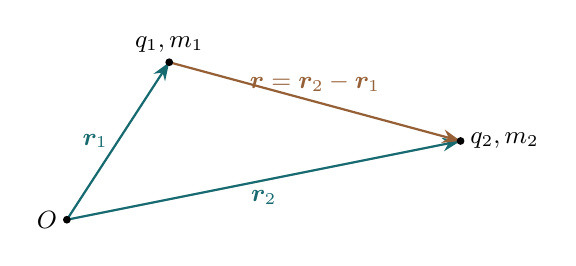
\begin{tikzpicture}[x=1cm,y=1cm]
\coordinate (O) at (0,0);\coordinate (A) at (1.3,2);\coordinate (B) at (5,1);
\draw[motion] (O)--(A) node[midway,left] {$\vect r_1$};\draw[motion] (O)--(B) node[midway,below] {$\vect r_2$};
\draw[force] (A)--(B) node[midway,above] {$\vect r=\vect r_2-\vect r_1$};
\foreach \p in {A,B,O}\fill (\p) circle (1.4pt);
\node[left] at (O) {$O$};\node[above] at (A) {$q_1,m_1$};\node[right] at (B) {$q_2,m_2$};
\end{tikzpicture}\figcaption{图 电1.1　相对位矢从电荷1指向电荷2。}\end{minipage}\end{center}

\Needspace{5\baselineskip}

\pdfbookmark[3]{题型定位}{q1-h0}

\subsection*{题型定位}

两体库仑相互作用下的质心与相对运动。由交换对称的两条运动方程引入约化质量，再从静止的零相对角动量初态求径向碰撞时间。

\Needspace{5\baselineskip}

\pdfbookmark[3]{知识点}{q1-h1}

\subsection*{知识点}

用从电荷1指向2的同一相对位矢写两力。两式相加给质心匀速，相减给相对方程；中央力使相对角动量守恒。异号时势能为 $-K/r$，能量给径向速率，靠近过程取 $\dot r<0$。


\Needspace{5\baselineskip}

\pdfbookmark[3]{物理图像}{q1-h2}

\subsection*{物理图像}

图电1.1的两位置矢量从同一 $O$ 出发。解图电1.1A中两力等大相向，静止质心 $C$ 将距离按质量反比分配。解图电1.1B的起始切线水平，随后随靠近变陡；前半间距约占总时间的 $81.8\%$。

\Needspace{5\baselineskip}

\pdfbookmark[3]{解题入口}{q1-h3}

\subsection*{解题入口}

将两条牛顿方程分别按质量除，再以电荷2加速度减去电荷1加速度。由相对角动量为零选固定方向的径向运动；写能量式并取负的距离导数，时间积分从 $r$ 到 $r_0$。

\Needspace{5\baselineskip}

\pdfbookmark[3]{标准解法}{q1-h4}

\subsection*{标准解法}

记$k=1/(4\pi\varepsilon_0)$，$r=|\vect r|$。题图中$\vect r$从电荷1指向电荷2，因而两条运动方程为
\[m_1\ddot{\vect r}_1=-\frac{kq_1q_2}{r^3}\vect r,\qquad
m_2\ddot{\vect r}_2=\frac{kq_1q_2}{r^3}\vect r.\]
第二式除以$m_2$，第一式除以$m_1$，再相减，得
\[\ddot{\vect r}=kq_1q_2\left(\frac1{m_1}+\frac1{m_2}\right)\frac{\vect r}{r^3}.\]
定义约化质量$\mu=m_1m_2/(m_1+m_2)$，相对运动方程便是
\result{\mu\ddot{\vect r}=\frac{kq_1q_2}{r^3}\vect r.}
这条矢量方程适用于任意初始速度；只有第二问给定的静止初态才保证两电荷此后沿初始连线运动。把两条运动方程相加还可得质心加速度为零；本题初始总动量为零，质心始终静止。
\begin{center}\begin{minipage}{0.97\linewidth}\centering
\begin{tikzpicture}[x=1cm,y=1cm]
\draw[guide] (-.5,0)--(6,0);\fill (0,0) circle (2pt) node[above] {$q_1$};\fill (5,0) circle (2pt) node[above] {$q_2$};
\fill (3,0) circle (1.5pt) node[above=5pt] {$C$};
\draw[force] (0,0)--(1.4,0) node[midway,below] {$\vect F_1$};\draw[force] (5,0)--(3.6,0) node[midway,below] {$\vect F_2$};
\draw[<->] (0,.85)--(5,.85) node[midway,above] {$r(t)$};
\node[below=22pt] at (3,0) {质心$C$静止，$\dot r<0$};
\end{tikzpicture}\figcaption{解图 电1.1A　异号电荷相向运动；质心将间距按质量反比分配。}\end{minipage}\end{center}
令$K=k|q_1q_2|>0$。在解图电1.1A所示的相向运动中，标量距离满足
\[\mu\ddot r=-\frac K{r^2},\qquad r(0)=r_0,\qquad\dot r(0)=0.\]
用$\ddot r=\dot r\,\dd\dot r/\dd r$积分，或直接写能量守恒，均得到
\[\frac12\mu\dot r^2-\frac K r=-\frac K{r_0},\qquad
\dot r=-\sqrt{\frac{2K}{\mu}\left(\frac1r-\frac1{r_0}\right)}.\]
负根对应距离随时间减小。把时间写成从当前间距$r$积到初始间距$r_0$，积分值为正：
\[t(r)=\sqrt{\frac{\mu}{2K}}\int_r^{r_0}\sqrt{\frac{r_0s}{r_0-s}}\,\dd s.\]
令$s=r_0\cos^2\theta$，则$\dd s=-2r_0\sin\theta\cos\theta\,\dd\theta$，而$r$对应
$\theta_r=\arccos\sqrt{r/r_0}$。于是
\begin{align*}
t(r)&=2\sqrt{\frac{\mu r_0^3}{2K}}\int_0^{\theta_r}\cos^2\theta\,\dd\theta\\
&=\sqrt{\frac{\mu r_0^3}{2K}}\left[\arccos\sqrt{\frac r{r_0}}+
\sqrt{\frac r{r_0}\left(1-\frac r{r_0}\right)}\right].
\end{align*}
取$r\to0$，得到相碰时间
\result{t_c=\frac\pi2\sqrt{\frac{\mu r_0^3}{2k|q_1q_2|}}
=\pi\sqrt{\frac{\pi\varepsilon_0\mu r_0^3}{2|q_1q_2|}}.}
在 $r=r_0$ 时，时间函数从零开始。由 $t_c\propto r_0^{3/2}$，初始间距加倍使相碰时间乘 $2^{3/2}$。若$m_2\to\infty$，$\mu\to m_1$，还原为电荷1向固定电荷2落下的情形。理想点电荷模型在$r=0$处速度发散，但上述时间积分收敛；这里的相碰时间指该理想模型达到零间距的极限。
\subsubsection*{质心、相对坐标和一维运动的条件}
令$M=m_1+m_2$，质心位置为
$\vect R_C=(m_1\vect r_1+m_2\vect r_2)/M$。
由两式相加得$M\ddot{\vect R}_C=0$，结合相对位矢可反解各自坐标：
\[
\vect r_1=\vect R_C-\frac{m_2}M\vect r,\qquad
\vect r_2=\vect R_C+\frac{m_1}M\vect r.
\]
因此解图电1.1A的C点把两电荷距离按质量反比分配，
静止释放时，两电荷在初始质心相碰。按图中从 $q_1$ 到 $q_2$ 的距离量取，质心位置为 $m_2r_0/M$，等质量时为 $r_0/2$。
相对运动的动量矩$\vect L=\mu\vect r\times\dot{\vect r}$守恒，
因为库仑力沿相对位矢、对相对原点的力矩为零。
本题静止初态给$\vect L=0$，结合中心力才保证连线方向固定，
从而可把矢量方程化为距离r的标量方程。
有非零相对角动量时还要联立极角变化，径向方程会出现角动量项。

动能分解也说明约化质量为何进入能量式：
\[
\frac12m_1|\dot{\vect r}_1|^2+\frac12m_2|\dot{\vect r}_2|^2
=\frac12M|\dot{\vect R}_C|^2+\frac12\mu|\dot{\vect r}|^2.
\]
初始两者均静止时第一项为零，所以相对能量就是全体系动能与相互作用势能之和。
若两者共同匀速平移，第一项为不变常数，相对运动与相碰时间仍相同。

\subsubsection*{用无量纲平方根换元完整复算时间积分}
对前面的时间积分另令$u=\sqrt{s/r_0}$，
有$s=r_0u^2$、$\dd s=2r_0u\dd u$，当前间距对应$u_r=\sqrt{r/r_0}$。
逐项代换得
\[
\begin{aligned}
t(r)&=\sqrt{\frac\mu{2K}}\int_r^{r_0}\sqrt{\frac{r_0s}{r_0-s}}\dd s\\
&=2\sqrt{\frac{\mu r_0^3}{2K}}\int_{u_r}^{1}\frac{u^2}{\sqrt{1-u^2}}\dd u.
\end{aligned}
\]
其中
\[
\int\frac{u^2}{\sqrt{1-u^2}}\dd u
=\frac12\left[\arcsin u-u\sqrt{1-u^2}\right]+C.
\]
代入上下限，令$\tau=\sqrt{\mu r_0^3/(2K)}$，便得
\[
t(r)=\tau\left[\frac\pi2-\arcsin\sqrt{\frac r{r_0}}
+\sqrt{\frac r{r_0}\left(1-\frac r{r_0}\right)}\right].
\]
利用$\pi/2-\arcsin u=\arccos u$，与三角换元结果完全相同。
靠近过程中 $\dot r<0$，用 $\dd t=\dd r/\dot r$ 换为从 $r$ 到 $r_0$ 的正向积分。起点 $r=r_0$ 时积分为零，靠近时积分区间随 $r$ 减小而增大。

\begin{center}\begin{minipage}{.97\linewidth}\centering
\begin{tikzpicture}[x=4.5cm,y=2.8cm,font=\small]
\draw[axis] (0,0)--(1.25,0) node[right] {$t/t_c$};
\draw[axis] (0,0)--(0,1.35) node[above] {$r/r_0$};
\draw[traj,domain=0:90,samples=130,variable=\t]
plot ({\t/90+sin(2*\t)/pi},{cos(\t)*cos(\t)});
\draw[guide] (.818309886,.5)--(0,.5) node[left] {$1/2$};
\draw[guide] (.818309886,0)--(.818309886,.5);
\node[below] at (1,0) {$1$};\node[left] at (0,1) {$1$};
\node at (.65,1.18) {$t_{1/2}/t_c=1/2+1/\pi$};
\end{tikzpicture}
\figcaption{解图 电1.1B　靠近速度逐渐增加，走完前一半间距占总时间约81.8\%。}
\end{minipage}\end{center}
解图电1.1B的初始切线水平，表示由静止释放；接近相碰时曲线越来越陡，
对应相对速率增长。靠近零间距时$|\dot r|\sim\sqrt{2K/(\mu r)}$，
故剩余时间积分按$\int_0^r\sqrt{s}\dd s$收敛，
约为$(2/3)\sqrt{\mu/(2K)}r^{3/2}$。
这段剩余时间按 $r^{3/2}$ 缩小，零间距在有限时刻达到。
若初始有非零相对角动量，径向有效势包含$L^2/(2\mu r^2)-K/r$，
零间距附近，正角动量项主导并使有效势趋于正无穷；有限能量的轨迹转向于正半径。


\Needspace{5\baselineskip}

\pdfbookmark[3]{关键洞察}{q1-h5}

\subsection*{关键洞察}

共同速度只改变质心轨迹。相对方程中的惯性系数为 $\mu$，静止初态的碰撞时间随 $r_0^{3/2}$ 增加。近零间距时，相对速度大小按 $r^{-1/2}$ 增加，因此经过剩余间距的时间按 $r^{3/2}$ 缩短。

\Needspace{5\baselineskip}

\pdfbookmark[3]{易错点}{q1-h6}

\subsection*{易错点}

相对位矢方向由图电1.1定义，排斥力或吸引力的正负由 $q_1q_2$ 给出。靠近时用负的距离导数及正向累积时间。每粒子从初态到质心的位移，由另一粒子的质量占总质量的比例确定。有切向相对速度时，径向方程要纳入角动量项。

\Needspace{5\baselineskip}

\pdfbookmark[3]{课堂讲解建议}{q1-h7}

\subsection*{课堂讲解建议}

先请一组相加求质心，一组相减求相对运动，再对照解图电1.1A识别各自坐标。引入共同速度，分别问相碰时刻和相碰位置怎样变化。写到能量平方根时让学生依据两箭头选择 $\dot r$ 的符号。

在解图电1.1B标出 $r_0/2$，把该点对应的时间和总时间比较。随后用变图电1.1V7引入一个切向初速，追问有效势曲线上哪一个点给相距最近的位置。

\Needspace{5\baselineskip}

\pdfbookmark[3]{变式训练}{q1-h8}

\subsection*{变式训练}

\begin{enumerate}
\item 两电荷具有同一初速度 $\vect V$。相减后相对初速度仍为零，所以在随质心匀速平移的坐标中，能量积分及 $t_c$ 保持。变图电1.1V1的中间箭头给出质心轨迹，末态两点在同一位置，因而
\[
\vect r_{\rm c}=\vect R_C(0)+\vect Vt_c .
\]
图中共同速度画成与初始连线垂直，沿连线的两个靠近距离仍按质量反比分配。
\begin{center}\begin{minipage}{.98\linewidth}\centering
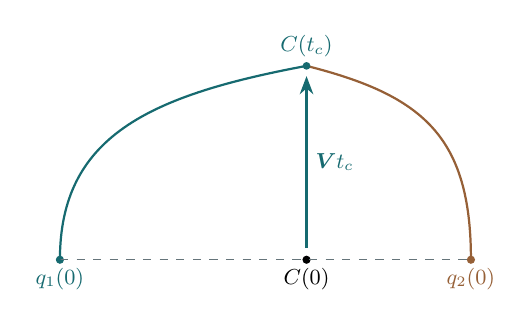
\begin{tikzpicture}[scale=.87,transform shape]
\fill[accent] (0,0)circle(1.7pt)node[below]{$q_1(0)$};\fill[warm](6,0)circle(1.7pt)node[below]{$q_2(0)$};\fill(3.6,0)circle(1.7pt)node[below]{$C(0)$};\draw[guide](0,0)--(6,0);\draw[motion](3.6,.17)--(3.6,2.68)node[midway,right]{$\vect Vt_c$};\draw[traj](0,0)..controls(0,1.8)and(1.3,2.40)..(3.6,2.83);\draw[warm,thick](6,0)..controls(6,1.8)and(5.3,2.4)..(3.6,2.83);\fill[accent](3.6,2.83)circle(1.6pt)node[above]{$C(t_c)$};
\end{tikzpicture}
\figcaption{变图 电1.1V1\quad 共同平移移动碰撞位置，曲线示意两电荷的轨迹}
\end{minipage}\end{center}
\item 间距第一次缩至 $r_0/2$ 时，三角换元的角为 $\theta_r=\pi/4$。代入时间式，
\[
t_{1/2}=\sqrt{\frac{\mu r_0^3}{2K}}\left(\frac{\pi}{4}+\frac12\right),
\qquad t_{1/2}/t_c=\frac12+\frac1\pi .
\]
变图电1.1V2在时间轴用两段刻尺显示，前半间距用时约 $0.8183t_c$，后半只有 $0.1817t_c$。两段间距相同，后半段靠近时的吸引加速度更大。
\begin{center}\begin{minipage}{.98\linewidth}\centering
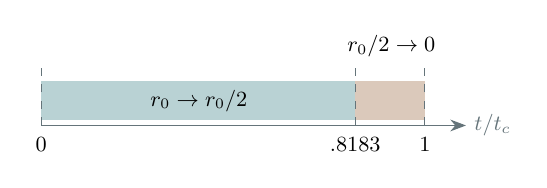
\begin{tikzpicture}[scale=.87,transform shape]
\draw[axis](0,.82)--(6.2,.82)node[right]{$t/t_c$};\fill[accent!30](0,.90)rectangle(4.582535,1.47);\fill[warm!34](4.582535,.90)rectangle(5.6,1.47);\foreach \x/\lab in {0/0,4.582535/.8183,5.6/1}{\draw[guide](\x,.82)--(\x,1.66);\node[below]at(\x,.77){\lab};}\node at(2.30,1.18){$r_0\to r_0/2$};\node[above]at(5.11,1.69){$r_0/2\to0$};
\end{tikzpicture}
\figcaption{变图 电1.1V2\quad 相同的两段间距在同一时间轴上占据不同长度}
\end{minipage}\end{center}
\item 两电荷同号且由静止释放，势能为 $K/r$，能量守恒给
\[
\frac12\mu\dot r^2=K\left(\frac1{r_0}-\frac1r\right).
\]
排斥使 $\dot r>0$。变图电1.1V3以 $r/r_0$ 为横坐标，速率从零上升，趋近 $v_*=\sqrt{2K/(\mu r_0)}$；无限远处相互作用能趋于零，初始正势能转化为相对动能。
\begin{center}\begin{minipage}{.98\linewidth}\centering
\begin{tikzpicture}[scale=.87,transform shape]
\draw[axis](0,0)--(6.18,0)node[right]{$r/r_0$};\draw[axis](0,0)--(0,3.42)node[above]{$v_{\rm rel}/v_*$};\draw[traj,domain=0:5.7,samples=72]plot(\x,{2.8*sqrt(max(0,1-1/(1+\x)))});\draw[guide](0,2.8)node[left]{1}--(5.7,2.8);\node[below]at(0,0){1};\node[below]at(3,0){4};
\end{tikzpicture}
\figcaption{变图 电1.1V3\quad 同号电荷分离时，相对速率趋于有限上限}
\end{minipage}\end{center}
\item 异号电荷在 $r_0$ 处已有向内相对速率 $v_0$，能量给
\[
\dot r=-\sqrt{v_0^2+\frac{2K}{\mu}\left(\frac1r-\frac1{r_0}\right)},\qquad
t_c=\int_0^{r_0}\frac{\dd r}{\sqrt{v_0^2+(2K/\mu)(1/r-1/r_0)}} .
\]
变图电1.1V4令 $\rho=r/r_0$、$\lambda=v_0/\sqrt{2K/(\mu r_0)}$，画出无量纲被积函数 $\sqrt{\rho/(1-\rho+\lambda^2\rho)}$。$\lambda$ 增大使曲线降低，面积即时间缩小。例取 $\lambda=1$，面积为 $\int_0^1\sqrt{\rho}\,\dd\rho=2/3$，是静止释放面积 $\pi/2$ 的 $4/(3\pi)$。
\begin{center}\begin{minipage}{.98\linewidth}\centering
\begin{tikzpicture}[scale=.87,transform shape]
\draw[axis](0,0)--(6.1,0)node[right]{$\rho$};\draw[axis](0,0)--(0,3.7)node[above]{无量纲被积函数};\draw[traj,domain=0:5.28,samples=72]plot(\x,{.51*sqrt((\x/5.4)/(1-\x/5.4))});\draw[traj,dashed,domain=0:5.40,samples=72]plot(\x,{.51*sqrt(\x/5.4)});\draw[guide](5.4,0)node[below]{1}--(5.4,3.50);\node[left]at(5.12,3.03){$\lambda=0$};\node[below left]at(5.12,.46){$\lambda=1$};\fill[accent](5.4,.51)circle(1.5pt);
\end{tikzpicture}
\figcaption{变图 电1.1V4\quad 初始靠近速率升高，使碰撞时间积分曲线的面积减小}
\end{minipage}\end{center}
\item 静止释放时，质心给相碰位置。沿图电1.1的相对位矢方向，两粒子的移动距离分别为 $m_2r_0/(m_1+m_2)$ 和 $m_1r_0/(m_1+m_2)$。变图电1.1V5以 $m_1:m_2=2:3$ 为例，左粒子走 $3r_0/5$，右粒子走 $2r_0/5$，在距左端 $0.6r_0$ 的质心相碰。如给整个系统共同速度 $\vect V$，最终位置还需加 $\vect Vt_c$。
\begin{center}\begin{minipage}{.98\linewidth}\centering
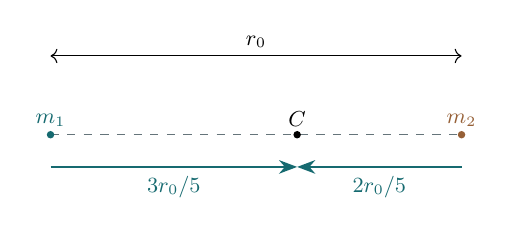
\begin{tikzpicture}[scale=.87,transform shape]
\draw[guide](0,1.12)--(6,1.12);\fill[accent](0,1.12)circle(1.55pt)node[above]{$m_1$};\fill[warm](6,1.12)circle(1.55pt)node[above]{$m_2$};\fill(3.6,1.12)circle(1.55pt)node[above]{$C$};\draw[motion](0,.65)--(3.6,.65)node[midway,below]{$3r_0/5$};\draw[motion](6,.65)--(3.6,.65)node[midway,below]{$2r_0/5$};\draw[<->](0,2.27)--(6,2.27)node[above,midway]{$r_0$};
\end{tikzpicture}
\figcaption{变图 电1.1V5\quad 质量为二比三时，静止质心距左端为总距离的五分之三}
\end{minipage}\end{center}
\item 设 $\rho=r/r_0$、$\tau=\sqrt{\mu r_0^3/(2K)}$、$v_*=\sqrt{2K/(\mu r_0)}$。由靠近支，当 $\rho\ll1$ 时，
\[
\frac{|\dot r|}{v_*}\sim \rho^{-1/2},\qquad
\frac{t_c-t}{\tau}\sim \int_0^\rho\sqrt u\,\dd u=\frac23\rho^{3/2}.
\]
变图电1.1V6两幅图分别看近零速度和剩余时间；左图随 $\rho$ 向零速度升高，右图的剩余时间趋于零。等价的有量纲式为 $t_c-t\sim(2/3)\sqrt{\mu/(2K)}r^{3/2}$。
\begin{center}\begin{minipage}{.98\linewidth}\centering
\begin{tikzpicture}[scale=.87,transform shape]
\draw[axis](0,0)--(2.9,0)node[right]{$\rho$};\draw[axis](0,0)--(0,3.18)node[above]{$|\dot r|/v_*$};\draw[traj,domain=0.22:2.55,samples=72]plot(\x,{.86/sqrt(\x/2.5)});\node[below]at(2.5,0){.05};\begin{scope}[xshift=4.26cm]\draw[axis](0,0)--(2.9,0)node[right]{$\rho$};\draw[axis](0,0)--(0,3.18)node[above]{$(t_c-t)/\tau$};\draw[traj,domain=0:2.55,samples=65]plot(\x,{3*pow(\x/2.5,1.5)});\node[below]at(2.5,0){.05};\end{scope}
\end{tikzpicture}
\figcaption{变图 电1.1V6\quad 两曲线表示近零间距的主导幂次}
\end{minipage}\end{center}
\item 设初始径向速度为零、具有切向相对速度，非零相对角动量 $L$ 使径向能量为
\[
E=\frac{\mu\dot r^2}{2}+U_{\rm eff}(r),\qquad
U_{\rm eff}=\frac{L^2}{2\mu r^2}-\frac Kr .
\]
变图电1.1V7取 $\sigma=L^2/(2\mu Kr_0)=0.18$，作出 $U_{\rm eff}/(K/r_0)=\sigma/\rho^2-1/\rho$。能量线为 $E/(K/r_0)=\sigma-1$；从 $\rho=1$ 向内运动，先遇到另一交点 $\rho=\sigma/(1-\sigma)\simeq0.2195$，此处 $\dot r=0$，是近心点。正的角动量项使有效势在零间距附近趋于正无穷。
\begin{center}\begin{minipage}{.98\linewidth}\centering
\begin{tikzpicture}[scale=.87,transform shape]
\draw[axis](0,0)--(6.1,0)node[right]{$\rho=r/r_0$};\draw[axis](0,0)--(0,4.0)node[above]{$U_{\rm eff}/(K/r_0)$};\draw[traj,domain=0.80:5.70,samples=72]plot(\x,{1.6*(.18/(\x/4.6)^2-1/(\x/4.6)+1.65)});\draw[guide](0,1.328)node[left]{$E/(K/r_0)$}--(5.68,1.328);\fill(1.009756,1.328)circle(1.55pt)node[above right]{近心点};\fill(4.6,1.328)circle(1.55pt);\draw[guide](4.6,0)node[below]{1}--(4.6,1.328);\node[left]at(0,2.64){0};
\end{tikzpicture}
\figcaption{变图 电1.1V7\quad 能量线在零间距之前与径向有效势相交}
\end{minipage}\end{center}
\item 若两物体在中心距 $d$ 处接触，而接触前仍用点电荷库仑力，运动到此刻即止。由主解的 $t(r)$ 取 $r=d$。变图电1.1V8的两个圆在中心间距 $d$ 时相切，图取 $d/r_0=1/4$，于是
\[
\frac{t(d)}{t_c}
=\frac2\pi\left(\arccos\sqrt{\frac14}+\sqrt{\frac14\frac34}\right)
=\frac23+\frac{\sqrt3}{2\pi}<1 .
\]
若有限尺寸也使电荷重新分布并改变力，则先按新的相互作用求能量，再将接触距离作为积分终点。
\begin{center}\begin{minipage}{.98\linewidth}\centering
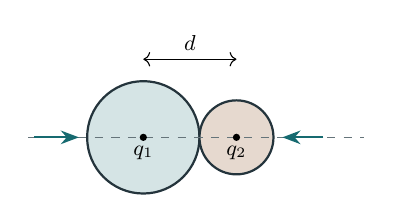
\begin{tikzpicture}[scale=.87,transform shape]
\draw[object,fill=accent!18](2.28,1.22)circle(.82);\draw[object,fill=warm!24](3.64,1.22)circle(.54);\draw[guide](.6,1.22)--(5.5,1.22);\fill(2.28,1.22)circle(1.5pt)node[below]{$q_1$};\fill(3.64,1.22)circle(1.5pt)node[below]{$q_2$};\draw[<->](2.28,2.36)--(3.64,2.36)node[above,midway]{$d$};\draw[motion](.69,1.22)--(1.34,1.22);\draw[motion](4.91,1.22)--(4.31,1.22);
\end{tikzpicture}
\figcaption{变图 电1.1V8\quad 到达正的接触距离时，库仑靠近积分停止}
\end{minipage}\end{center}
\end{enumerate}

\clearpage

\pdfbookmark[2]{第 2 题 正方形中心电荷的小振动}{q2}

\section*{第 2 题\quad 正方形中心电荷的小振动}\label{q:2}

边长为$a$的正方形四个顶点各固定一个电量为$Q$的点电荷。中心放一个质量为$m$、电量为$q$的自由点电荷，$qQ>0$。将它沿一条对角线移动很小的距离后由静止释放。判断它是否作周期性振动；若是，求小振动周期，并说明稳定性的空间范围。

\begin{center}\begin{minipage}{0.97\linewidth}\centering
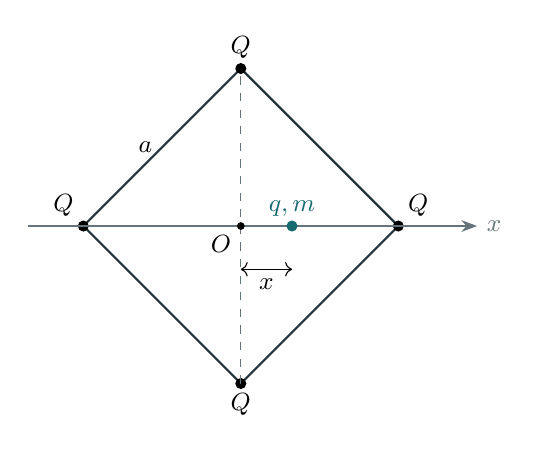
\begin{tikzpicture}[x=1cm,y=1cm]
\draw[object] (-2,0)--(0,2)--(2,0)--(0,-2)--cycle;
\foreach \x/\y in {-2/0,0/2,2/0,0/-2}\fill (\x,\y) circle (2pt);\node[above left] at (-2,0) {$Q$};\node[above] at (0,2) {$Q$};\node[above right] at (2,0) {$Q$};\node[below] at (0,-2) {$Q$};
\draw[axis] (-2.7,0)--(3,0) node[right] {$x$};\draw[guide] (0,-2)--(0,2);
\fill (0,0) circle (1.4pt) node[below left] {$O$};\fill[accent] (.65,0) circle (2pt) node[above] {$q,m$};
\node[left] at (-1,1) {$a$};\draw[<->] (0,-.55)--(.65,-.55) node[midway,below] {$x$};
\end{tikzpicture}\figcaption{图 电1.2　沿水平对角线释放电荷，四个顶点电荷固定。}\end{minipage}\end{center}

\Needspace{5\baselineskip}

\pdfbookmark[3]{题型定位}{q2-h0}

\subsection*{题型定位}

从四顶点电荷的库仑力求对角线小振动。平面内和面外分别由势能曲率判断稳定性；再由四阶项求有限小振幅下的首阶周期修正。

\Needspace{5\baselineskip}

\pdfbookmark[3]{知识点}{q2-h1}

\subsection*{知识点}

半对角线 $b=a/\sqrt2$。沿运动线的一对给 $-4kqQx/b^3$，另一对给 $+2kqQx/b^3$。相加后由线性回复系数求频率。平面内的二阶势能只含 $x^2+y^2$，面外的二阶项变号，构成鞍点。


\Needspace{5\baselineskip}

\pdfbookmark[3]{物理图像}{q2-h2}

\subsection*{物理图像}

解图电1.2A中，右顶点近、左顶点远，二者合成左向力；上、下两个顶点的竖直分力相消，水平分力都向右。解图电1.2B把沿对角线的势阱与法线上的势垒顶部画在一起。

\Needspace{5\baselineskip}

\pdfbookmark[3]{解题入口}{q2-h3}

\subsection*{解题入口}

在图电1.2中按两对固定电荷分组。沿轴一对比较 $b+x$ 和 $b-x$；另一对的水平投影是 $x/\sqrt{b^2+x^2}$。相加求线性系数，再以面外力或二阶势能判断法向。有限振幅用真实势能写四分之一周期积分。

\Needspace{5\baselineskip}

\pdfbookmark[3]{标准解法}{q2-h4}

\subsection*{标准解法}

记正方形半对角线长$b=a/\sqrt2$，取所移对角线为$x$轴。电荷$q$位于$(x,0)$，$|x|\ll b$。对角线上的两个固定电荷位于$(\pm b,0)$；另一对位于$(0,\pm b)$。以下令$k=1/(4\pi\varepsilon_0)$。
\begin{center}\begin{minipage}{0.97\linewidth}\centering
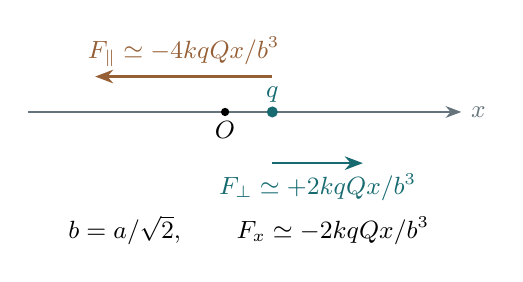
\begin{tikzpicture}[x=1cm,y=1cm]
\draw[axis] (-2.5,0)--(3,0) node[right] {$x$};\fill (0,0) circle (1.5pt) node[below] {$O$};
\fill[accent] (.6,0) circle (2pt) node[above] {$q$};
\draw[force] (.6,.45)--(-1.65,.45) node[midway,above] {$F_{\parallel}\simeq-4kqQx/b^3$};
\draw[motion] (.6,-.65)--(1.75,-.65) node[midway,below] {$F_{\perp}\simeq+2kqQx/b^3$};
\node at (.3,-1.5) {$b=a/\sqrt2,\qquad F_x\simeq-2kqQx/b^3$};
\end{tikzpicture}\figcaption{解图 电1.2A　两组顶点电荷的水平合力方向相反，左向回复项较大。}\end{minipage}\end{center}
解图电1.2A把两组顶点电荷的轴向合力分别画出：沿运动对角线的一组给向左的$-4kqQx/b^3$，垂直对角线的一组给向右的$+2kqQx/b^3$。按同一轴向相加，左向项有一半被右向项抵消，余下的回复系数决定振动频率。

沿$x$轴的一对电荷产生的合力为
\begin{align*}
F_{\parallel}&=kqQ\left[\frac1{(b+x)^2}-\frac1{(b-x)^2}\right]\\
&=\frac{kqQ}{b^2}\left[\left(1+\frac xb\right)^{-2}-\left(1-\frac xb\right)^{-2}\right]
=-\frac{4kqQ}{b^3}x+O(x^3).
\end{align*}
上、下两个电荷的竖直分量相互抵消。每个电荷到$q$的距离为$\sqrt{b^2+x^2}$，其水平投影因子为$x/\sqrt{b^2+x^2}$，所以
\[F_{\perp}=\frac{2kqQx}{(b^2+x^2)^{3/2}}
=\frac{2kqQ}{b^3}x+O(x^3).\]
两组相加，得到小位移下的运动方程
\[m\ddot x=-\frac{2kqQ}{b^3}x,\qquad
\omega^2=\frac{2kqQ}{mb^3}=\frac{\sqrt2\,qQ}{\pi\varepsilon_0ma^3}.\]
因为$qQ>0$，线性项为回复力。沿对角线静止释放时，由对称性运动始终保持在该直线上，小振动近似为简谐运动，其周期为
\result{T=2\pi\sqrt{\frac{mb^3}{2kqQ}}
=\pi\sqrt{\frac{2\sqrt2\,\pi\varepsilon_0ma^3}{qQ}}.}
这个周期是振幅趋于零时的极限；有限振幅的首个修正在后文由完整势能求出。

沿面外法线作位移时，回复力的符号随方向改变。利用正方形的旋转对称性，平面内任意方向的一阶合力均为$-2kqQ\vect r_{\parallel}/b^3$，故平面内稳定。若使电荷向垂直平面的$z$方向移动，则四个电荷的$z$分量同向：
\[F_z=\frac{4kqQz}{(b^2+z^2)^{3/2}}\simeq\frac{4kqQ}{b^3}z.\]
法向力沿位移方向，故法向微扰增长。题设沿严格对角线静止释放时，对称性保持这一条轨迹。
\subsubsection*{势能鞍点与平面内的线性各向同性}
设一般小位移为 $(x,y,z)$，记其长度为 $s$。四个固定电荷到中心的距离都是 $b$。固定电荷关于中心成对布置，势能展开中的奇次项相消，因此
\[
U(x,y,z)=\frac{4kqQ}{b}
+\frac{kqQ}{b^3}(x^2+y^2-2z^2)
+O\left(\frac{k|qQ|}{b}\left(\frac{s}{b}\right)^4\right).
\]
因此势能在x、y方向曲率相同且为正，z方向曲率为负，
Hessian矩阵为$[2kqQ/b^3]\operatorname{diag}(1,1,-2)$。
三个曲率之和为零，与中心附近没有固定电荷的拉普拉斯方程相容。
平面内任意小位移的一阶恢复力相同，
法向曲率为负，中心在三维势能面上为鞍点。

\begin{center}\begin{minipage}{.97\linewidth}\centering
\begin{tikzpicture}[x=6cm,y=5cm,font=\small]
\draw[axis] (-.43,0)--(.48,0) node[right] {$\xi=x/b\text{或}z/b$};
\draw[axis] (0,-.32)--(0,.34) node[above] {$\Delta U/(kqQ/b)$};
\draw[traj,domain=-.35:.35,samples=120] plot(\x,{1/(1-\x)+1/(1+\x)+2/sqrt(1+\x*\x)-4});
\draw[brown,thick,dashed,domain=-.35:.35,samples=120] plot(\x,{4/sqrt(1+\x*\x)-4});
\node at (.23,.25) {沿对角线};\node at (.23,-.29) {沿面外法线};
\node[left] at (0,.2) {$0.2$};\node[left] at (0,-.2) {$-0.2$};
\end{tikzpicture}
\figcaption{解图 电1.2B　同一归一位移下，沿对角线为势阱，沿面外法线为势垒顶部。}
\end{minipage}\end{center}
解图电1.2B两曲线对应同一套四顶点电荷，
实线沿给定对角线取$U(x,0,0)$，虚线沿垂直轴取$U(0,0,z)$。
它们在原点都斜率为零，但曲率相反，于是沿对角线的力指向原点，沿法线的力指向远离原点。
在小振动近似中平面内x、y具有同一频率，
严格沿对角线由静止释放时，对称性还保证横向坐标一直为零。
平面内的高阶势能项依赖方向，所以一般方向的有限振幅轨迹还包含横向偏转。

\subsubsection*{有限振幅的首个周期修正}
沿题设对角线，在$|x|<b$范围完整势能为
\[
U(x)=kqQ\left[\frac1{b-x}+\frac1{b+x}+\frac2{\sqrt{b^2+x^2}}\right].
\]
继续保留四阶项，
\[
U(x)=\frac{4kqQ}b+\frac{kqQ}{b^3}x^2
+\frac{11kqQ}{4b^5}x^4+O(x^6),
\quad F_x=-\frac{2kqQ}{b^3}x-\frac{11kqQ}{b^5}x^3+O(x^5).
\]
三次回复项为负，表明这条方向上的回复力随振幅增强。
若从振幅A静止释放，能量差可写成
\[
\frac12m\dot x^2=\frac{kqQ}{b^3}(A^2-x^2)
\left[1+\frac{11}{4b^2}(A^2+x^2)+O(A^4/b^4)\right].
\]
令$x=A\sin\phi$代入四分之一周期积分，按$A/b$展开，得到
\[
\frac{T(A)}{T_0}
=\frac2\pi\int_0^{\pi/2}\left[1+\frac{11A^2}{4b^2}(1+\sin^2\phi)\right]^{-1/2}\dd\phi
+O(A^4/b^4)
=1-\frac{33}{16}\frac{A^2}{b^2}+O(A^4/b^4).
\]
这里$T_0$为前面求得的小振动周期。
在 $A\ll b$ 的范围内，周期比零振幅极限略短。若释放点接近顶点，应用前面的完整势能积分。


\Needspace{5\baselineskip}

\pdfbookmark[3]{关键洞察}{q2-h5}

\subsection*{关键洞察}

二阶势能的三个曲率与 $(1,1,-2)$ 成比例。平面内两方向具有相同小振动频率，法向斜率使离开中心的微扰扩大。沿给定对角线的四阶势能系数为正，首个周期修正为负。

\Needspace{5\baselineskip}

\pdfbookmark[3]{易错点}{q2-h6}

\subsection*{易错点}

把边长换成半对角线再计算各力。来自上下顶点的力取水平投影，符号与靠近的顶点一对相反。平面内等频只说明小位移的线性方程；法向力和有限振幅分别使用各自的势能与相应近似。

\Needspace{5\baselineskip}

\pdfbookmark[3]{课堂讲解建议}{q2-h7}

\subsection*{课堂讲解建议}

首先在图电1.2上画四个力，请学生按方向抵消一对竖直分量，然后解释两项为什么随同一个 $x$ 增长却符号相反。求出周期后，将 $q$ 沿法线移动很小距离，在解图电1.2B上对应曲线的切线方向。

再沿对角线逐项展开到三次力，指出投影一组的线性与三次项符号不同。用变图电1.2V6比较小振幅周期和完整势能积分，进而用变图电1.2V8讨论加机械回复力后法向曲率的变化。

\Needspace{5\baselineskip}

\pdfbookmark[3]{变式训练}{q2-h8}

\subsection*{变式训练}

\begin{enumerate}
\item 中心电荷与顶点异号时，所有势能项改变符号。变图电1.2V1画出归一化二阶势能沿对角线和法线的两支。对角线的势能二次项变为 $-k|qQ|x^2/b^3$，所以
\[
F_x\simeq+2k|qQ|x/b^3,
\]
离开中心后继续偏离。法线上的二次项为 $+2k|qQ|z^2/b^3$，提供回复力。三维中心仍是鞍点。
\begin{center}\begin{minipage}{.98\linewidth}\centering
\begin{tikzpicture}[scale=.87,transform shape]
\draw[axis](-3.1,0)--(3.55,0)node[right]{$x/b$ 或 $z/b$};\draw[axis](0,-1.50)--(0,2.72)node[above]{$\Delta U/(k|qQ|/b)$};\draw[traj,domain=-2.82:2.82,samples=72]plot(\x,{-.13333*\x*\x});\draw[traj,dashed,domain=-2.82:2.82,samples=72]plot(\x,{.26666*\x*\x});\node[right]at(2.55,1.80){法向势阱};\node[right]at(2.60,-.92){平面内};
\end{tikzpicture}
\figcaption{变图 电1.2V1\quad 异号时，稳定与失稳方向同号情形互换}
\end{minipage}\end{center}
\item 若异号电荷被严格约束在法线上，四个顶点到它等距，轴向力为 $-4k|qQ|z/(b^2+z^2)^{3/2}$。小位移给
\[
m\ddot z=-4k|qQ|z/b^3,\qquad
T_z=2\pi\sqrt{\frac{mb^3}{4k|qQ|}} .
\]
变图电1.2V2画出若从正 $z$ 轴释放，四个吸引力的横向分量成对抵消，法向分量一致向下。与同等 $|qQ|$ 的原对角线周期相比，$T_z=T_0/\sqrt2$。
\begin{center}\begin{minipage}{.98\linewidth}\centering
\begin{tikzpicture}[scale=.87,transform shape]
\draw[axis](0,-.16)--(0,3.88)node[above]{$z$};\draw[object](-2,0)--(0,-.53)--(2,0)--(0,.53)--cycle;\foreach \x/\y in {-2/0,0/-.53,2/0,0/.53}{\fill(\x,\y)circle(1.5pt);}\fill[accent](0,2.85)circle(1.65pt)node[above right]{$q$};\draw[force](0,2.85)--(-1.16,1.20);\draw[force](0,2.85)--(1.16,1.20);\draw[force](0,2.85)--(0,1.49)node[midway,right]{$F_z$};\node[below right]at(2,0){四个顶点所在平面};
\end{tikzpicture}
\figcaption{变图 电1.2V2\quad 法线上吸引力的合力沿轴指回中心}
\end{minipage}\end{center}
\item 同号电荷在平面内沿与对角线成 $30^\circ$ 的方向微移。二阶势能为 $kqQ(x^2+y^2)/b^3$，故
\[
\vect F_\parallel=-\frac{2kqQ}{b^3}(x\vect e_x+y\vect e_y).
\]
变图电1.2V3画出位移与力同线反向，任意平面方位的一阶振动有同一个周期。有限振幅时，四阶势能包含方向因素，应从实际位移计算横向力。
\begin{center}\begin{minipage}{.98\linewidth}\centering
\begin{tikzpicture}[scale=.87,transform shape]
\draw[axis](-.56,0)--(4.45,0)node[right]{$x$};\draw[axis](0,-.43)--(0,3.45)node[above]{$y$};\draw[guide](0,0)circle(2.8);\fill[accent]({2.8*cos(30)},{2.8*sin(30)})circle(1.55pt)node[above right]{$q$};\draw[motion](0,0)--({2.8*cos(30)},{2.8*sin(30)})node[above left,midway]{$\vect r_\parallel$};\draw[force]({2.52*cos(30)},{2.52*sin(30)})--({.89*cos(30)},{.89*sin(30)})node[below right,midway]{$\vect F_\parallel$};\draw(.72,0)arc(0:30:.72);\node at(1.2,.22){$30^\circ$};
\end{tikzpicture}
\figcaption{变图 电1.2V3\quad 平面内线性回复力沿位移的反方向}
\end{minipage}\end{center}
\item 四顶点的电量都变为 $2Q$，边长变为 $2a$，则半对角线也变为 $2b$。回复系数从 $2kqQ/b^3$ 变为
\[
\frac{2kq(2Q)}{(2b)^3}=\frac14\frac{2kqQ}{b^3} .
\]
变图电1.2V4的两条直线分别表示相同位移下的线性回复力大小，斜率缩为四分之一。中心电荷质量保持时，$\omega$ 变为原来的一半，周期变为 $2T_0$。
\begin{center}\begin{minipage}{.98\linewidth}\centering
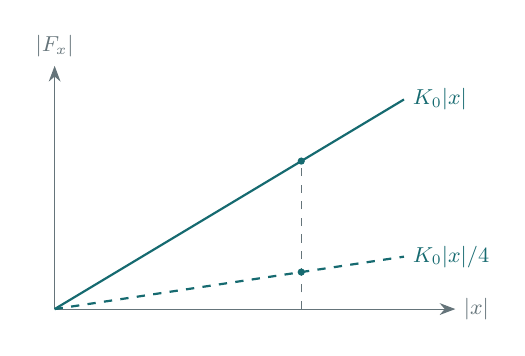
\begin{tikzpicture}[scale=.87,transform shape]
\draw[axis](0,0)--(5.85,0)node[right]{$|x|$};\draw[axis](0,0)--(0,3.55)node[above]{$|F_x|$};\draw[traj](0,0)--(5.1,3.06)node[right]{$K_0|x|$};\draw[traj,dashed](0,0)--(5.1,.765)node[right]{$K_0|x|/4$};\draw[guide](3.6,0)--(3.6,2.16);\fill[accent](3.6,2.16)circle(1.5pt);\fill[accent](3.6,.54)circle(1.5pt);
\end{tikzpicture}
\figcaption{变图 电1.2V4\quad 距离增大体现为三次方减弱，电量增加只乘一次方}
\end{minipage}\end{center}
\item 沿对角线把两组力展开到三次：
\[
F_{\parallel}=\frac{kqQ}{b^2}(-4u-8u^3)+O(u^5),\qquad
F_{\perp}=\frac{kqQ}{b^2}(2u-3u^3)+O(u^5),\quad u=x/b.
\]
变图电1.2V5先减去各自的线性项。对 $u>0$，两条曲线都向负方向弯，三次系数分别为 $-8,-3$。相加得 $F_x=-(kqQ/b^2)(2u+11u^3)+O(u^5)$，可见两组力的线性作用相反，三次项却同向。
\begin{center}\begin{minipage}{.98\linewidth}\centering
\begin{tikzpicture}[scale=.87,transform shape]
\draw[axis](0,3.02)--(6.08,3.02)node[right]{$u$};\draw[axis](0,.16)--(0,3.57)node[above]{$\Delta F/(kqQ/b^2)$};\draw[traj,domain=0:5.42,samples=72]plot(\x,{3.02-8*8*(\x/16)^3});\draw[traj,dashed,domain=0:5.42,samples=72]plot(\x,{3.02-8*3*(\x/16)^3});\node[above right]at(4.77,2.30){垂直一对};\node[below left]at(5.38,.57){沿轴一对};\node[left]at(0,3.02){0};\node[above]at(4.8,3.02){0.3};
\end{tikzpicture}
\figcaption{变图 电1.2V5\quad 从两组力中减去线性项后，三次贡献均为负}
\end{minipage}\end{center}
\item 从振幅 $A$ 静止释放时，能量给 $m\dot x^2/2=U(A)-U(x)$。将 $x=A\sin\phi$ 代入四分之一周期，按 $A/b$ 展开，有
\[
\frac{T(A)}{T_0}=1-\frac{33A^2}{16b^2}+O(A^4/b^4).
\]
变图电1.2V6用实线表示完整势能的积分值，用虚线表示只留振幅平方项。两线在 $A/b$ 很小时贴合，说明沿这条对称线周期随振幅先缩短；比较其他方向的有限振幅，要从对应方向的势能重新展开。
\begin{center}\begin{minipage}{.98\linewidth}\centering
\begin{tikzpicture}[scale=.87,transform shape]
\draw[axis](0,0)--(6.0,0)node[right]{$A/b$};\draw[axis](0,0)--(0,3.35)node[above]{$T/T_0$};\draw[traj]plot coordinates {(0.00000,2.800000) (0.11250,2.798854) (0.22500,2.795420) (0.33750,2.789704) (0.45000,2.781720) (0.56250,2.771485) (0.67500,2.759020) (0.78750,2.744353) (0.90000,2.727514) (1.01250,2.708539) (1.12500,2.687466) (1.23750,2.664340) (1.35000,2.639205) (1.46250,2.612112) (1.57500,2.583111) (1.68750,2.552258) (1.80000,2.519608) (1.91250,2.485221) (2.02500,2.449155) (2.13750,2.411471) (2.25000,2.372232) (2.36250,2.331499) (2.47500,2.289334) (2.58750,2.245801) (2.70000,2.200960) (2.81250,2.154873) (2.92500,2.107602) (3.03750,2.059205) (3.15000,2.009741) (3.26250,1.959268) (3.37500,1.907841) (3.48750,1.855515) (3.60000,1.802342) (3.71250,1.748372) (3.82500,1.693655) (3.93750,1.638237) (4.05000,1.582163) (4.16250,1.525477) (4.27500,1.468218) (4.38750,1.410426) (4.50000,1.352136) (4.61250,1.293385) (4.72500,1.234203) (4.83750,1.174622) (4.95000,1.114671) (5.06250,1.054375) (5.17500,0.993759) (5.28750,0.932846) (5.40000,0.871657)};\draw[traj,dashed,domain=0:5.4,samples=72]plot(\x,{8*(1-33*(\x/13.5)^2/16-.65)});\node[left]at(0,2.8){1};\node[left]at(0,0){.65};\node[below]at(5.4,0){.4};\node[above]at(4.22,1.65){完整势能};\node[below left]at(5.45,.23){二次近似};
\end{tikzpicture}
\figcaption{变图 电1.2V6\quad 小振幅时周期缩短，完整积分与首项修正逐渐分开}
\end{minipage}\end{center}
\item 中心处的势能二阶矩阵为
\[
\frac{2kqQ}{b^3}\operatorname{diag}(1,1,-2).
\]
曲率之和为零。令 $\omega_0^2=2kqQ/(mb^3)$，则 $x$ 方向满足 $\ddot x=-\omega_0^2 x$，法向满足 $\ddot z=2\omega_0^2 z$。从静止小位移释放后，变图电1.2V7的左式给 $x/x_0=\cos(\omega_0t)$，右式给 $z/z_0=\cosh(\sqrt2\omega_0t)$；两式体现中心势能的鞍形。
\begin{center}\begin{minipage}{.98\linewidth}\centering
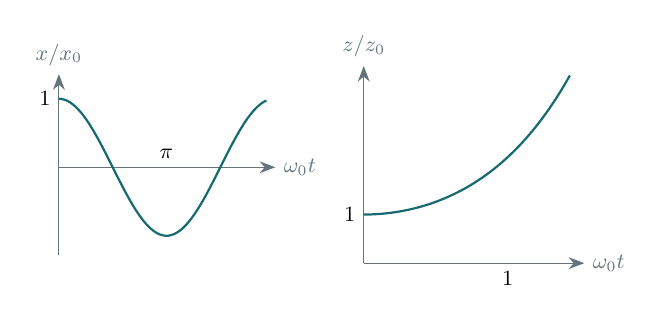
\begin{tikzpicture}[scale=.87,transform shape]
\draw[axis](0,1.40)--(3.16,1.40)node[right]{$\omega_0t$};\draw[axis](0,.12)--(0,2.76)node[above]{$x/x_0$};\draw[traj,domain=0:3.03,samples=73]plot(\x,{1.40+cos(deg(2*\x))});\node[left]at(0,2.4){1};\node[above]at(1.5708,1.4){$\pi$};\begin{scope}[xshift=4.45cm]\draw[axis](0,0)--(3.22,0)node[right]{$\omega_0t$};\draw[axis](0,0)--(0,2.88)node[above]{$z/z_0$};\draw[traj,domain=0:3.01,samples=73]plot(\x,{.355*(exp(sqrt(2)*\x/2.10)+exp(-sqrt(2)*\x/2.10))});\node[left]at(0,.71){1};\node[below]at(2.10,0){1};\end{scope}
\end{tikzpicture}
\figcaption{变图 电1.2V7\quad 平面内小位移周期变化，法向小扰动随时间增大}
\end{minipage}\end{center}
\item 若额外施加法向机械势 $m\Omega^2z^2/2$，总二阶曲率为 $m\Omega^2-4kqQ/b^3$。变图电1.2V8用
\[
\Omega_c^2=\frac{4kqQ}{mb^3}
\]
作尺度。$\Omega>\Omega_c$ 时法向具有线性回复力，小振动角频率为 $\sqrt{\Omega^2-\Omega_c^2}$；$\Omega<\Omega_c$ 时法向仍不稳定。恰在等号时二阶项相消，库仑势的下一项是 $3kqQz^4/(2b^5)$，在法线上仍产生非线性回复。机械势改变了总曲率。
\begin{center}\begin{minipage}{.98\linewidth}\centering
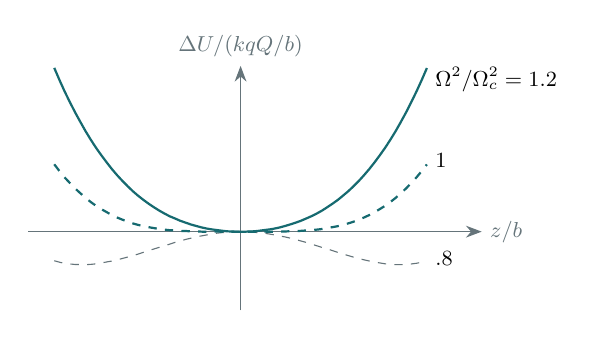
\begin{tikzpicture}[scale=.87,transform shape]
\draw[axis](-3.1,1.20)--(3.52,1.20)node[right]{$z/b$};\draw[axis](0,.05)--(0,3.62)node[above]{$\Delta U/(kqQ/b)$};\draw[guide,domain=-2.72:2.72,samples=72]plot(\x,{1.20+16*(4/sqrt(1+(\x/5.8)^2)-4+2*.8*(\x/5.8)^2)});\draw[traj,dashed,domain=-2.72:2.72,samples=72]plot(\x,{1.20+16*(4/sqrt(1+(\x/5.8)^2)-4+2*(\x/5.8)^2)});\draw[traj,domain=-2.72:2.72,samples=72]plot(\x,{1.20+16*(4/sqrt(1+(\x/5.8)^2)-4+2*1.2*(\x/5.8)^2)});\node[right]at(2.72,3.42){$\Omega^2/\Omega_c^2=1.2$};\node[right]at(2.72,2.24){1};\node[right]at(2.72,.81){.8};
\end{tikzpicture}
\figcaption{变图 电1.2V8\quad 外加法向二次势改变中心曲率，等号时由四次项回复}
\end{minipage}\end{center}
\end{enumerate}

\clearpage

\pdfbookmark[2]{第 3 题 共线四点电荷作用下的轴向运动}{q3}

\section*{第 3 题\quad 共线四点电荷作用下的轴向运动}\label{q:3}

在$x$轴的$x=\pm a$处各固定一个电量为$Q$的点电荷，在$x=\pm2a$处各固定一个电量为$-8Q$的点电荷，$Q>0$。电量为$q>0$、质量为$m$的质点只能沿$x$轴运动。判断原点$O$是否为稳定平衡位置。若稳定，将质点移至$x=A$处静止释放，$0<A\ll a$，求振动周期的主阶表达式。

\begin{center}\begin{minipage}{0.97\linewidth}\centering
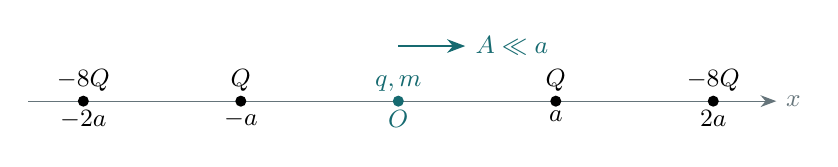
\begin{tikzpicture}[x=1cm,y=1cm]
\draw[axis] (-4.7,0)--(4.8,0) node[right] {$x$};
\foreach \x/\t/\p in {-4/{-8Q}/{-2a},-2/Q/{-a},2/Q/a,4/{-8Q}/{2a}}{\fill (\x,0) circle (2pt);\node[above] at (\x,0) {$\t$};\node[below] at (\x,0) {$\p$};}
\fill[accent] (0,0) circle (2pt) node[above] {$q,m$} node[below] {$O$};
\draw[motion] (0,.7)--(.85,.7) node[right] {$A\ll a$};
\end{tikzpicture}\figcaption{图 电1.3　四个固定电荷共线排列，活动电荷限制在该直线上运动。}\end{minipage}\end{center}

\Needspace{5\baselineskip}

\pdfbookmark[3]{题型定位}{q3-h0}

\subsection*{题型定位}

线性项相消后的非线性振动。先用最低非零的三次力判断平衡，再按四次势能将能量积分化为振幅尺度乘无量纲积分。

\Needspace{5\baselineskip}

\pdfbookmark[3]{知识点}{q3-h1}

\subsection*{知识点}

电荷关于原点成对布置，轴向力为奇函数。近、远两对一次项相消，三次项合为 $-\beta x^3$。位能为 $\beta x^4/4$，速率由 $A^4-x^4$ 决定；令 $x/A=\cos\phi$ 后，四分之一周期可用第一类椭圆积分表达。


\Needspace{5\baselineskip}

\pdfbookmark[3]{物理图像}{q3-h2}

\subsection*{物理图像}

图电1.3中 $q$ 向右移，近处同号电荷给左向力，远处异号电荷给右向力。解图电1.3A的四次势阱在中心较平，能量线与曲线交于 $\pm A$。振幅减小时，回复力按振幅的三次方衰减，因此一周时间变长。

\Needspace{5\baselineskip}

\pdfbookmark[3]{解题入口}{q3-h3}

\subsection*{解题入口}

先列四项有符号力，将 $2a$ 的距离用于远处电荷并统一用 $u=x/a$ 展开。一次项消去后，继续取同奇次的三次项。对力积分得势能，由 $x=A$ 到 $x=0$ 的能量式求四分之一周期。

\Needspace{5\baselineskip}

\pdfbookmark[3]{标准解法}{q3-h4}

\subsection*{标准解法}

先写$|x|<a$内的有符号合力。两侧$Q$排斥$q$，两侧$-8Q$吸引$q$，所以
\[F_x=kqQ\left[\frac1{(a+x)^2}-\frac1{(a-x)^2}
-\frac8{(2a+x)^2}+\frac8{(2a-x)^2}\right].\]
用$u=x/a$展开，保留到三次项：
\begin{align*}
\frac{a^2F_x}{kqQ}
&=(1+u)^{-2}-(1-u)^{-2}
-2(1+u/2)^{-2}+2(1-u/2)^{-2}\\
&=(-4u-8u^3)+\left(4u+2u^3\right)+O(u^5)\\
&=-6u^3+O(u^5).
\end{align*}
一次项恰好抵消，但三次项未消失。因此
\[F_x\simeq-\beta x^3,\qquad \beta=\frac{6kqQ}{a^5}=\frac{3qQ}{2\pi\varepsilon_0a^5}>0.\]
两个对称电荷对的准确合力还可写成 $4akqQx[16/(4a^2-x^2)^2-1/(a^2-x^2)^2]$。在 $0<|x|<a$ 时，$4(a^2-x^2)<4a^2-x^2$，因此方括号为负，回复力的方向与位移相反。原点的一阶斜率为零，最低阶的回复项为上面得到的三次项。
\begin{center}\begin{minipage}{0.97\linewidth}\centering
\begin{tikzpicture}[x=2.4cm,y=2cm,font=\small]
\draw[axis] (-1.4,0)--(1.55,0) node[right] {$\xi=x/A$};
\draw[axis] (0,-.1)--(0,1.75) node[above] {$U/(\beta A^4/4)$};
\draw[traj,domain=-1.1:1.1,samples=120] plot(\x,{pow(\x,4)});
\draw[guide] (-1,1)--(1,1);\draw[guide] (-1,0) node[below] {$-1$}--(-1,1);
\draw[guide] (1,0) node[below] {$1$}--(1,1);\node[left] at (0,1) {$1$};
\node at (-.75,1.6) {$U/E=\xi^4$};\draw[force] (.65,.15)--(.25,.15);
\end{tikzpicture}\figcaption{解图 电1.3A　原点是四次势阱底部；能量线在两个转折点截出往复范围。}\end{minipage}\end{center}
解图电1.3A画出原点附近的平坦势阱，转折点的高度决定运动能量。取$U(0)=0$，在三次回复力近似下
\[U(x)=-\int_0^xF_x(s)\,\dd s=\frac\beta4x^4.\]
从$x=A$静止释放后，能量守恒给出
\[\frac12m\dot x^2+\frac\beta4x^4=\frac\beta4A^4,
\qquad |\dot x|=\sqrt{\frac\beta{2m}(A^4-x^4)}.\]
图中从$A$运动到$0$恰为四分之一周期，因此
\[T=4\sqrt{\frac{2m}{\beta}}\int_0^A\frac{\dd x}{\sqrt{A^4-x^4}}
=\frac4A\sqrt{\frac{2m}{\beta}}\int_0^1\frac{\dd u}{\sqrt{1-u^4}}.\]
这是有限的反常积分。若用第一类完全椭圆积分
\[\mathsf K(\kappa)=\int_0^{\pi/2}\frac{\dd\phi}{\sqrt{1-\kappa^2\sin^2\phi}},\]
令$u=\cos\phi$，则
\[\int_0^1\frac{\dd u}{\sqrt{1-u^4}}
=\int_0^{\pi/2}\frac{\dd\phi}{\sqrt{1+\cos^2\phi}}
=\frac1{\sqrt2}\mathsf K(1/\sqrt2).\]
由$\mathsf K(1/\sqrt2)\approx1.854074677$得到
\result{T\simeq\frac4A\sqrt{\frac m\beta}\,\mathsf K(1/\sqrt2)
\approx\frac{7.41630}{A}\sqrt{\frac{2\pi\varepsilon_0ma^5}{3qQ}}.}
$A\ll a$保证被略去的五次力项相对三次项为$O(A^2/a^2)$，上式是周期的主阶近似。随振幅减小，周期按 $A^{-1}$ 增大，频率趋零。三次回复力使往复运动呈非简谐。
\subsubsection*{四次势能下的稳定平衡与任意位置的到达时间}
解图电1.3A中最低非零势能项为正的$\beta x^4/4$。
从任意充分小振幅A静止释放，总能量为$\beta A^4/4$，
能量守恒使$|x|\le A$，所以小扰动不会使质点远离原点。
正的四次势能项使有限小能量的运动始终局限在原点附近，故原点为稳定平衡。
在$A=0$时，质点保持静止；
$T\to\infty$描述的是一族非零振幅轨道的极限。

还可保留第一类不完全椭圆积分，描述从A到任意x的运动。
定义
\[
\mathsf F(\Phi,\kappa)=\int_0^\Phi
\frac{\dd\phi}{\sqrt{1-\kappa^2\sin^2\phi}},\qquad
\mathsf K(\kappa)=\mathsf F(\pi/2,\kappa).
\]
对$0\le x\le A$，令$s=A\cos\phi$，两因子分开后有
\[
\begin{aligned}
\int_x^A\frac{\dd s}{\sqrt{(A^2+s^2)(A^2-s^2)}}
&=\int_0^{\arccos(x/A)}\frac{\dd\phi}{\sqrt{A^2+A^2\cos^2\phi}}\\
&=\frac1{\sqrt2A}\mathsf F\left(\arccos\frac xA,\frac1{\sqrt2}\right).
\end{aligned}
\]
因此第一段从A向原点运动的时间为
\[
t(x)=\frac1A\sqrt{\frac m\beta}
\mathsf F\left(\arccos\frac xA,\frac1{\sqrt2}\right).
\]
取$x=0$得$T/4$，再用奇偶对称延续到其余三段，恢复完整周期。
从A到0的时间乘4才给完整周期；其余位置的到达时间则保留不完全积分的上限。
定义中$\kappa$是模数；若计算工具使用参数$\kappa^2$，此处应输入$1/2$。

\subsubsection*{振幅缩放、平均能量与被略去项}
令$y=x/A$，$\tau=A\sqrt{\beta/m}\,t$，
三次回复方程化为
\[
\frac{\dd^2y}{\dd\tau^2}+y^3=0,\qquad
y(0)=1,\quad y'(0)=0.
\]
归一运动与A无关，故物理时间尺度必与$A^{-1}$成正比，
最大速度与$A^2$成正比，最大加速度与$A^3$成正比。
四次势能使回复力按位移三次方变化，因此振幅改变时频率也随之改变。

若需要平均动能，用周期平均的
$\langle\dd(xm\dot x)/\dd t\rangle=0$，
得$2\langle E_k\rangle=4\langle U\rangle$，
所以$\langle E_k\rangle=2E/3$、$\langle U\rangle=E/3$。
四次势阱中，平均动能为平均势能的两倍。

完整电场继续展开给
\[
F_x=-\frac{6kqQ}{a^5}x^3
-\frac{45kqQ}{4a^7}x^5+O(x^7).
\]
在$|x|\le A$上，五次项相对三次项不超过主阶的$(15/8)A^2/a^2$。
这给忽略高次力的具体尺度，周期的主阶误差仍为$O(A^2/a^2)$。
若远处电荷略偏离$-8Q$而恢复一次项，
在足够小的振幅下运动又会由线性项主导；线性项和三次项的相对大小同时取决于参数偏差和振幅。


\Needspace{5\baselineskip}

\pdfbookmark[3]{关键洞察}{q3-h5}

\subsection*{关键洞察}

四次势阱有严格极小，能量限制小扰动留在原点附近。频率随振幅趋零与稳定相容：严格 $A=0$ 是静止解，$T\propto1/A$ 描述非零振幅轨道。无量纲方程还给 $v_{\max}\propto A^2,a_{\max}\propto A^3$。

\Needspace{5\baselineskip}

\pdfbookmark[3]{易错点}{q3-h6}

\subsection*{易错点}

远处电荷的距离是 $2a$，改用 $u$ 后展开量为 $u/2$。从 $A$ 到 $0$ 的时间乘4才得一周；椭圆积分的模数为 $1/\sqrt2$，参数记法下输入 $1/2$。在整个往复段的最大振幅处比较五次力和三次力，便可估计忽略五次项的相对大小。

\Needspace{5\baselineskip}

\pdfbookmark[3]{课堂讲解建议}{q3-h7}

\subsection*{课堂讲解建议}

让学生算出两对电荷的一次项，再问需要展开到哪一阶判方向。根据解图电1.3A的水平线，标出两个转折点和四分之一周期的路径。先用 $x=Au$ 读出周期的振幅比例，再写椭圆积分的换元。

最后将外电荷改成 $-\eta Q$，画出变图电1.3V8的两项等强线。通过比较该线上下的受力，让学生说明 $\eta$ 接近8时，线性周期适用的振幅怎样随参数缩小。

\Needspace{5\baselineskip}

\pdfbookmark[3]{变式训练}{q3-h8}

\subsection*{变式训练}

\begin{enumerate}
\item 将外电荷改成 $-\eta Q$。从近、远两对的距离分别展开，得
\[
F_x=\frac{kqQ}{a^3}(-4+\eta/2)x+O(x^3).
\]
变图电1.3V1取 $\eta=6,8,10$ 对比中心处的曲线。$\eta<8$ 时一次项为负，给线性回复；$\eta>8$ 时为正，使小位移增大。$\eta=8$ 时线性斜率为零，近原点由三次负项恢复。
\begin{center}\begin{minipage}{.98\linewidth}\centering
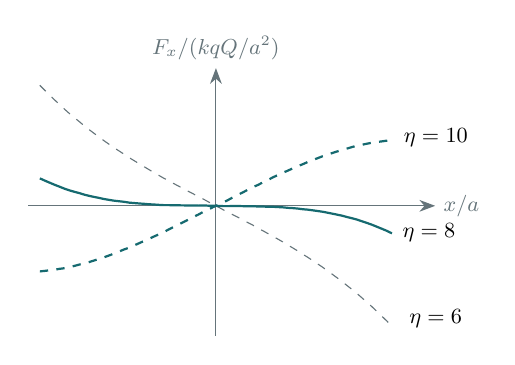
\begin{tikzpicture}[scale=.87,transform shape]
\draw[axis](-2.74,0)--(3.2,0)node[right]{$x/a$};\draw[axis](0,-1.9)--(0,2.01)node[above]{$F_x/(kqQ/a^2)$};\draw[guide,domain=-2.57:2.57,samples=72]plot(\x,{6.2*(pow(1+\x/12,-2)-pow(1-\x/12,-2)-1.5*pow(1+\x/24,-2)+1.5*pow(1-\x/24,-2))});\draw[traj,domain=-2.57:2.57,samples=72]plot(\x,{6.2*(pow(1+\x/12,-2)-pow(1-\x/12,-2)-2*pow(1+\x/24,-2)+2*pow(1-\x/24,-2))});\draw[traj,dashed,domain=-2.57:2.57,samples=72]plot(\x,{6.2*(pow(1+\x/12,-2)-pow(1-\x/12,-2)-2.5*pow(1+\x/24,-2)+2.5*pow(1-\x/24,-2))});\node[right]at(2.7,-1.65){$\eta=6$};\node[right]at(2.60,-.39){$\eta=8$};\node[right]at(2.62,.99){$\eta=10$};
\end{tikzpicture}
\figcaption{变图 电1.3V1\quad 改变远处电荷后，中心处的一次斜率经过零}
\end{minipage}\end{center}
\item 当 $\eta<8$ 且振幅足够小，线性回复系数为 $K=(kqQ/a^3)(4-\eta/2)$，周期
\[
T=2\pi\sqrt{\frac{ma^3}{kqQ(4-\eta/2)}}.
\]
变图电1.3V2画出 $T$ 除以 $\eta=0$ 的周期后得到的 $(1-\eta/8)^{-1/2}$。$\eta$ 接近8时图上周期增长，同时需进一步减小振幅以让一次力主导；在 $\eta=8$ 处，任一给定小非零振幅的周期由四次势能计算。
\begin{center}\begin{minipage}{.98\linewidth}\centering
\begin{tikzpicture}[scale=.87,transform shape]
\draw[axis](0,0)--(6.1,0)node[right]{$\eta$};\draw[axis](0,0)--(0,3.7)node[above]{$T_{\rm lin}/T_{\eta=0}$};\draw[traj,domain=0:5.19,samples=72]plot(\x,{.83/sqrt(1-\x/5.55)});\draw[guide](5.55,0)node[below]{8}--(5.55,3.52);\node[left]at(0,.83){1};\node[below]at(2.775,0){4};
\end{tikzpicture}
\figcaption{变图 电1.3V2\quad 接近一次项相消时，线性振动的时间尺度增大}
\end{minipage}\end{center}
\item 四次势能给最大速度出现在 $x=0$，由能量
\[
v_{\max}=A^2\sqrt{\frac{\beta}{2m}} .
\]
变图电1.3V3把振幅缩半前后的速度和周期分别归一化，得到 $v_{\max}'/v_{\max}=1/4$ 及 $T'/T=2$。速度下降得比行程缩短更快，所以一周用时反而增大。
\begin{center}\begin{minipage}{.98\linewidth}\centering
\begin{tikzpicture}[scale=.87,transform shape]
\draw[axis](0,0)--(5.97,0)node[right]{振幅};\draw[axis](0,0)--(0,3.82)node[above]{各量的相对值};\fill[accent!28](.75,0)rectangle(1.42,1.56);\fill[warm!39](1.55,0)rectangle(2.22,1.56);\fill[accent!28](3.62,0)rectangle(4.29,.39);\fill[warm!39](4.42,0)rectangle(5.09,3.12);\node[above]at(1.085,1.56){1};\node[above]at(1.885,1.56){1};\node[above]at(3.955,.39){$1/4$};\node[above]at(4.755,3.12){2};\node[below]at(1.485,0){$A$};\node[below]at(4.355,0){$A/2$};\node at(2.68,3.35){浅色：速率，深色：周期};
\end{tikzpicture}
\figcaption{变图 电1.3V3\quad 振幅减半使最大速率降至四分之一，周期加倍}
\end{minipage}\end{center}
\item 若回复力为 $F=-cx^{2n-1}$，其中 $c>0$ 且 $n$ 为正整数，势能为 $cx^{2n}/(2n)$。从振幅 $A$ 静止出发，
\[
T=4\sqrt{\frac{mn}{c}}\, A^{1-n}
\int_0^1\frac{\dd u}{\sqrt{1-u^{2n}}}.
\]
变图电1.3V4以各自 $A_*$ 处周期归一化，画出 $T(A)/T(A_*)=(A/A_*)^{1-n}$。$n=1$ 等时，$n=2$ 为本题反比，$n=3$ 随小振幅增长得更快。
\begin{center}\begin{minipage}{.98\linewidth}\centering
\begin{tikzpicture}[scale=.87,transform shape]
\draw[axis](0,0)--(6.12,0)node[right]{$A/A_*$};\draw[axis](0,0)--(0,3.86)node[above]{$T/T(A_*)$};\draw[guide,domain=1.75:5.48,samples=72]plot(\x,{.86});\draw[traj,domain=1.75:5.48,samples=72]plot(\x,{.86*3.15/\x});\draw[traj,dashed,domain=1.75:5.48,samples=72]plot(\x,{.86*(3.15/\x)^2});\draw[guide](3.15,0)node[below]{1}--(3.15,.86)--(0,.86)node[left]{1};\fill(3.15,.86)circle(1.4pt);\node[above]at(1.96,2.50){$n=3$};\node[above]at(2.42,1.15){$n=2$};\node[right]at(5.49,.86){$n=1$};
\end{tikzpicture}
\figcaption{变图 电1.3V4\quad 力的次数改变零振幅附近的时间尺度}
\end{minipage}\end{center}
\item 从 $A$ 静止释放后到 $x=A/2$，取 $x=A\cos\Phi$，故 $\Phi=\pi/3$。时间为
\[
t=\frac1A\sqrt{\frac m\beta}\,\mathsf F\!\left(\frac\pi3,\frac1{\sqrt2}\right).
\]
变图电1.3V5的横轴以 $T/4$ 为单位，半振幅对应
\[
\frac{t}{T/4}
=\frac{\mathsf F(\pi/3,1/\sqrt2)}{\mathsf K(1/\sqrt2)}
\simeq 0.6162.
\]
起点附近曲线较平，靠近原点时斜率绝对值增大，正对应四次势阱中的变速运动。
\begin{center}\begin{minipage}{.98\linewidth}\centering
\begin{tikzpicture}[scale=.87,transform shape]
\draw[axis](0,0)--(6.13,0)node[right]{$t/(T/4)$};\draw[axis](0,0)--(0,3.63)node[above]{$x/A$};\draw[traj]plot coordinates {(0.000000,3.000000) (0.076960,2.998972) (0.153946,2.995889) (0.230984,2.990752) (0.308102,2.983566) (0.385326,2.974335) (0.462681,2.963065) (0.540195,2.949765) (0.617894,2.934443) (0.695805,2.917110) (0.773954,2.897777) (0.852369,2.876459) (0.931075,2.853170) (1.010099,2.827924) (1.089469,2.800741) (1.169212,2.771639) (1.249353,2.740636) (1.329921,2.707756) (1.410941,2.673020) (1.492441,2.636451) (1.574448,2.598076) (1.656987,2.557920) (1.740086,2.516012) (1.823770,2.472379) (1.908065,2.427051) (1.992997,2.380060) (2.078591,2.331438) (2.164870,2.281218) (2.251859,2.229434) (2.339580,2.176123) (2.428056,2.121320) (2.517307,2.065064) (2.607354,2.007392) (2.698213,1.948344) (2.789902,1.887961) (2.882436,1.826284) (2.975828,1.763356) (3.070087,1.699219) (3.165222,1.633917) (3.261238,1.567496) (3.358138,1.500000) (3.455920,1.431476) (3.554580,1.361971) (3.654110,1.291533) (3.754498,1.220210) (3.855727,1.148050) (3.957776,1.075104) (4.060619,1.001421) (4.164228,0.927051) (4.268566,0.852046) (4.373595,0.776457) (4.479270,0.700336) (4.585541,0.623735) (4.692356,0.546707) (4.799657,0.469303) (4.907382,0.391579) (5.015466,0.313585) (5.123841,0.235377) (5.232437,0.157008) (5.341181,0.078531) (5.450000,0.000000)};\draw[guide](3.358137858506509,0)node[below]{0.6162}--(3.358137858506509,1.5)--(0,1.5)node[left]{$1/2$};\node[left]at(0,3){1};\node[below]at(5.45,0){1};\fill[accent](3.358137858506509,1.5)circle(1.5pt);
\end{tikzpicture}
\figcaption{变图 电1.3V5\quad 半振幅所用时间由不完全积分与完全积分的比值给出}
\end{minipage}\end{center}
\item 对周期轨道的 $xm\dot x$ 作一周平均。由于一周末回到初始状态，其导数平均为零，且
\[
\frac{\dd}{\dd t}(xm\dot x)=m\dot x^2+xF=2E_k-4U.
\]
故 $2\langle E_k\rangle=4\langle U\rangle$，与 $\langle E_k\rangle+\langle U\rangle=E$ 联立得 $2E/3$ 与 $E/3$。变图电1.3V6画出一段从转折点到原点的能量交换；四段的能量平均相同，图中两水平线给整个周期的相应均值。
\begin{center}\begin{minipage}{.98\linewidth}\centering
\begin{tikzpicture}[scale=.87,transform shape]
\draw[axis](0,0)--(6.13,0)node[right]{$t/(T/4)$};\draw[axis](0,0)--(0,3.64)node[above]{能量$/E$};\draw[traj]plot coordinates {(0.000000,3.000000) (0.076960,2.995890) (0.153946,2.983588) (0.230984,2.963179) (0.308102,2.934801) (0.385326,2.898648) (0.462681,2.854966) (0.540195,2.804050) (0.617894,2.746242) (0.695805,2.681929) (0.773954,2.611538) (0.852369,2.535532) (0.931075,2.454407) (1.010099,2.368686) (1.089469,2.278915) (1.169212,2.185660) (1.249353,2.089498) (1.329921,1.991014) (1.410941,1.890797) (1.492441,1.789432) (1.574448,1.687500) (1.656987,1.585566) (1.740086,1.484181) (1.823770,1.383873) (1.908065,1.285144) (1.992997,1.188469) (2.078591,1.094288) (2.164870,1.003006) (2.251859,0.914987) (2.339580,0.830558) (2.428056,0.750000) (2.517307,0.673550) (2.607354,0.601402) (2.698213,0.533702) (2.789902,0.470553) (2.882436,0.412012) (2.975828,0.358093) (3.070087,0.308769) (3.165222,0.263971) (3.261238,0.223595) (3.358138,0.187500) (3.455920,0.155515) (3.554580,0.127441) (3.654110,0.103053) (3.754498,0.082106) (3.855727,0.064340) (3.957776,0.049481) (4.060619,0.037248) (4.164228,0.027356) (4.268566,0.019520) (4.373595,0.013462) (4.479270,0.008910) (4.585541,0.005606) (4.692356,0.003309) (4.799657,0.001797) (4.907382,0.000871) (5.015466,0.000358) (5.123841,0.000114) (5.232437,0.000023) (5.341181,0.000001) (5.450000,0.000000)};\draw[traj,dashed]plot coordinates {(0.000000,0.000000) (0.076960,0.004110) (0.153946,0.016412) (0.230984,0.036821) (0.308102,0.065199) (0.385326,0.101352) (0.462681,0.145034) (0.540195,0.195950) (0.617894,0.253758) (0.695805,0.318071) (0.773954,0.388462) (0.852369,0.464468) (0.931075,0.545593) (1.010099,0.631314) (1.089469,0.721085) (1.169212,0.814340) (1.249353,0.910502) (1.329921,1.008986) (1.410941,1.109203) (1.492441,1.210568) (1.574448,1.312500) (1.656987,1.414434) (1.740086,1.515819) (1.823770,1.616127) (1.908065,1.714856) (1.992997,1.811531) (2.078591,1.905712) (2.164870,1.996994) (2.251859,2.085013) (2.339580,2.169442) (2.428056,2.250000) (2.517307,2.326450) (2.607354,2.398598) (2.698213,2.466298) (2.789902,2.529447) (2.882436,2.587988) (2.975828,2.641907) (3.070087,2.691231) (3.165222,2.736029) (3.261238,2.776405) (3.358138,2.812500) (3.455920,2.844485) (3.554580,2.872559) (3.654110,2.896947) (3.754498,2.917894) (3.855727,2.935660) (3.957776,2.950519) (4.060619,2.962752) (4.164228,2.972644) (4.268566,2.980480) (4.373595,2.986538) (4.479270,2.991090) (4.585541,2.994394) (4.692356,2.996691) (4.799657,2.998203) (4.907382,2.999129) (5.015466,2.999642) (5.123841,2.999886) (5.232437,2.999977) (5.341181,2.999999) (5.450000,3.000000)};\draw[guide](0,2)node[left]{$2/3$}--(5.45,2);\draw[guide](0,1)node[left]{$1/3$}--(5.45,1);\node[above right]at(5.28,2.99){$E_k/E$};\node[above]at(.79,2.94){$U/E$};\node[below]at(5.45,0){1};
\end{tikzpicture}
\figcaption{变图 电1.3V6\quad 四次势阱中的平均动能为总能量的三分之二}
\end{minipage}\end{center}
\item 下一非零项为 $F_5=-45kqQx^5/(4a^7)$，三次力为 $F_3=-6kqQx^3/a^5$。因此
\[
|F_5/F_3|=\frac{15}{8}\frac{x^2}{a^2},
\quad \max_{|x|\le A}|F_5/F_3|=\frac{15}{8}\frac{A^2}{a^2}.
\]
变图电1.3V7把整个运动区间的最大相对项画成振幅的函数，如 $A/a=0.20$ 时为0.075。将含五次力的势能与振幅定义一致地放入能量积分，可见周期的相对误差也从 $O(A^2/a^2)$ 起。
\begin{center}\begin{minipage}{.98\linewidth}\centering
\begin{tikzpicture}[scale=.87,transform shape]
\draw[axis](0,0)--(6.13,0)node[right]{$A/a$};\draw[axis](0,0)--(0,3.55)node[above]{最大 $|F_5/F_3|$};\draw[traj,domain=0:5.50,samples=72]plot(\x,{12*(15/8)*(\x/15)^2});\draw[guide](3,0)node[below]{.20}--(3,.9)--(0,.9)node[left]{.075};\fill(3,.9)circle(1.5pt);
\end{tikzpicture}
\figcaption{变图 电1.3V7\quad 五次项相对三次项的最大比例发生在转折点}
\end{minipage}\end{center}
\item 接近且小于 $\eta=8$ 时，三次项为 $-(kqQ/a^5)(8-\eta/4)x^3$。在最大位移处比较两项，线性周期适用需
\[
(8-\eta/4)\frac{A^2}{a^2}\ll4-\eta/2.
\]
变图电1.3V8以 $\delta=8-\eta$ 为横轴，两项等强时 $A^2/a^2=\delta/(12+\delta/2)$。线性近似用在该线下方较远处；接近 $\eta=8$ 时条件成为 $A^2/a^2\ll(8-\eta)/12$。例如 $\eta=7.9$ 时，两项等强的振幅约为 $0.0911a$，要由一次项主导还需再取较小的振幅。
\begin{center}\begin{minipage}{.98\linewidth}\centering
\begin{tikzpicture}[scale=.87,transform shape]
\draw[axis](0,0)--(6.05,0)node[right]{$\delta=8-\eta$};\draw[axis](0,0)--(0,3.82)node[above]{$A^2/a^2$};\draw[traj,domain=0:5.30,samples=72]plot(\x,{78*(\x/13)/(12+.5*\x/13)});\fill[accent](1.3,.64730)circle(1.5pt);\draw[guide](1.3,0)node[below]{.10}--(1.3,.64730);\node[above left]at(4.15,3.11){两项等强};\node[below right]at(3.28,1.39){线性项较大};
\end{tikzpicture}
\figcaption{变图 电1.3V8\quad 接近精确抵消时，能沿用线性周期的振幅随参数减小}
\end{minipage}\end{center}
\end{enumerate}

\clearpage

\pdfbookmark[2]{第 4 题 反平方律与带电球壳的内场}{q4}

\section*{第 4 题\quad 反平方律与带电球壳的内场}\label{q:4}

证明：若真空中的电力严格服从反平方律，一个孤立带电导体球壳达到静电平衡时，电荷均匀分布在外表面，球壳内部电场处处为零。球形空腔内没有电荷，外部没有其他电荷或外加电场。说明证明中反平方律起什么作用。

\begin{center}\begin{minipage}{0.97\linewidth}\centering
\begin{tikzpicture}[x=1cm,y=1cm]
\fill[accent!10] (0,0) circle (1.9);\fill[white] (0,0) circle (1.45);\draw[object] (0,0) circle (1.9);\draw[object] (0,0) circle (1.45);
\fill (0,0) circle (1pt) node[below] {$O$};\fill (.55,.5) circle (1.5pt) node[above] {$P$};
\foreach \t in {0,45,...,315}\node at (\t:2.08) {$+$};
\node[right,align=left] at (2.8,.35) {球形空腔内无电荷\\外部无其他电荷};
\end{tikzpicture}\figcaption{图 电1.4　孤立导体球壳的静电平衡；图示取总电荷为正。}\end{minipage}\end{center}

\Needspace{5\baselineskip}

\pdfbookmark[3]{题型定位}{q4-h0}

\subsection*{题型定位}

由反平方律证明均匀球壳内场为零，再构造孤立导体的静电平衡并证明唯一。

\Needspace{5\baselineskip}

\pdfbookmark[3]{知识点}{q4-h1}

\subsection*{知识点}

对面元的投影立体角为 $\dd S\cos\alpha/s^2$。球弦两端法线与弦的锐角相同，近、远面积与距离平方成正比。球面势连续，面电荷给法向场跳变。孤立导体的差势能量积分由表面常差势与总电荷差相乘。


\Needspace{5\baselineskip}

\pdfbookmark[3]{物理图像}{q4-h2}

\subsection*{物理图像}

解图电1.4A中偏心点 $P$ 到两面元的距离不同，较远面元在同一细双锥内占更大面积。反平方衰减使这两面元给 $P$ 的场等大反向。解图电1.4B的内侧势为水平段，外侧按 $1/s$ 下降。

\Needspace{5\baselineskip}

\pdfbookmark[3]{解题入口}{q4-h3}

\subsection*{解题入口}

在已知均匀带电的球面上取任意内点 $P$。用球心到弦的垂足说明两个角相同，写下相等的立体角并代入面元场。然后将总电荷均匀放到导体外球面，证明其满足金属及空腔的等势条件，最后用差势说明唯一。

\Needspace{5\baselineskip}

\pdfbookmark[3]{标准解法}{q4-h4}

\subsection*{标准解法}

先在已知均匀带电的球面上计算内场。再用所得零场构造导体的等势状态，最后说明这种分布的唯一性。
\begin{center}\begin{minipage}{0.97\linewidth}\centering
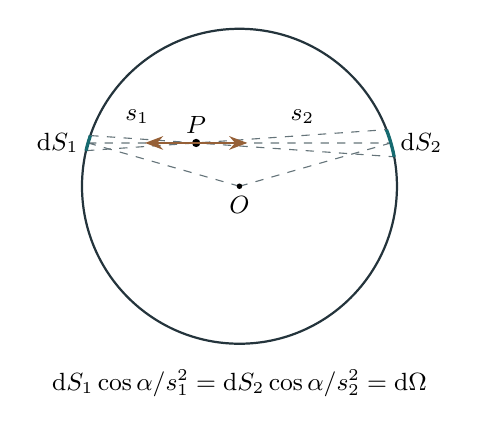
\begin{tikzpicture}[x=1cm,y=1cm,font=\small]
\draw[object] (0,0) circle(2);
\coordinate (O) at (0,0);\coordinate (P) at (-.55,.55);
\coordinate (A) at (-1.922888452303,0.550000000000);\coordinate (B) at (1.922888452303,0.550000000000);

\draw[guide] (A)--(B) (O)--(A) (O)--(B);
\draw[guide] (-1.893497532617,0.643946499310)--(1.964690175953,0.374155732970);
\draw[guide] (-1.948201642550,0.452228216682)--(1.866303874830,0.718964426654);
\draw[very thick,accent] (161.217699286521:2) arc[start angle=161.217699286521,end angle=166.931599616959,radius=2];
\draw[very thick,accent] (10.782300713479:2) arc[start angle=10.782300713479,end angle=21.068400383041,radius=2];

\fill (O) circle(1pt) node[below] {$O$};\fill (P) circle(1.5pt) node[above] {$P$};
\node[left] at (A) {$\dd S_1$};\node[right] at (B) {$\dd S_2$};
\node[above] at (-1.3,.67) {$s_1$};\node[above] at (.8,.67) {$s_2$};
\draw[force] (P)--(.1,.55);\draw[force] (P)--(-1.2,.55);
\node at (0,-2.5) {$\dd S_1\cos\alpha/s_1^2=\dd S_2\cos\alpha/s_2^2=\dd\Omega$};
\end{tikzpicture}\figcaption{解图 电1.4A　同一细双锥两端的面元对P张相同立体角；近面元小、远面元大。}\end{minipage}\end{center}
先考虑半径为$R$、表面电荷密度为常量$\sigma$的薄球面。在内部任取一点$P$；在解图电1.4A中，通过$P$取一个很细的双锥，两端截得面元$\dd S_1,\dd S_2$，到$P$的距离分别为$s_1,s_2$。过球心$O$向这条弦作垂线，垂足把弦平分。两端点与$O$、垂足组成全等直角三角形，所以两端球面法线与弦的锐角相同，记为$\alpha$。两个面元对$P$张相同的立体角，故
\[\dd\Omega=\frac{\dd S_1\cos\alpha}{s_1^2}
=\frac{\dd S_2\cos\alpha}{s_2^2},\qquad
\frac{\dd S_1}{s_1^2}=\frac{\dd S_2}{s_2^2}.\]
依据反平方律，两面元在$P$的场强大小分别为
\[\dd E_1=k|\sigma|\frac{\dd S_1}{s_1^2},\qquad
\dd E_2=k|\sigma|\frac{\dd S_2}{s_2^2}.\]
它们大小相等、方向相反，逐对抵消。让细双锥遍历半个立体角空间，恰好将球面配对一次，因此
\result{\vect E(P)=0\qquad (|OP|<R).}
对任意内部点都可作这样的细双锥；球心处也可直接按对径点配对。

\Needspace{10\baselineskip}
现在回到总电荷为$Q_{\rm tot}$的孤立导体球壳。把全部电荷均匀放在外表面，令
\[\sigma_{\rm out}=\frac{Q_{\rm tot}}{4\pi R_{\rm out}^2},\qquad
\sigma_{\rm in}=0.\]
刚才的球壳结果表明，这一分布在金属内部和空腔内部都给出零电场；外表面等势，满足静电平衡。它也是唯一的平衡分布：对于给定孤立导体总电荷、无内部电荷且无外加场的边界条件，静电场的唯一性排除了另一个不同分布。也可在确定平衡解唯一后，由旋转对称性说明外表面电荷密度必须处处相同。

反平方律与上述面元的几何比例恰好相配。作为比较，若假设力随$s^{-(2+\delta)}$变化，可引入固定长度$\ell$使比例系数的量纲不变。对预先给定的同一均匀带电球面，两面元的场强差含有因子
\[\dd E_{\rm pair}=\frac{k\sigma\,\dd\Omega}{\cos\alpha}
\left[\left(\frac\ell{s_1}\right)^\delta-\left(\frac\ell{s_2}\right)^\delta\right],\]
其中正方向取从近面元一侧指向远面元一侧，图示按$\sigma>0$说明。$\delta=0$时逐对严格抵消；$\delta\ne0$时一般不再如此。偏心内场因而可用于比较距离指数。这里球面电荷分布预先给定；若电荷还能移动，需按所用的力律及导体条件联立确定其分布。
\subsubsection*{由球面电荷积分求内外两侧的电势}
对半径R的固定均匀带电球面，令$s=|OP|$，取OP为积分极轴。
面元到P距离为$\sqrt{R^2+s^2-2Rs\cos\theta}$，
把纬圈电量$\sigma\,2\pi R^2\sin\theta\dd\theta$逐项代入电势，得
\[
\varphi(s)=2\pi k\sigma R^2\int_{-1}^{1}
\frac{\dd u}{\sqrt{R^2+s^2-2Rsu}}
=\frac{2\pi k\sigma R}{s}[(R+s)-|R-s|].
\]
内点$s<R$时绝对值为$R-s$，所以
\[
\varphi(s)=4\pi k\sigma R=\frac{kQ_{\rm tot}}R;
\qquad s>R\text{时},\quad\varphi(s)=\frac{kQ_{\rm tot}}s.
\]
球心用$s\to0$的极限得到同一内势。
解图电1.4B画出这一连续的内外电势：内侧水平段给零梯度，
外侧按$1/s$下降；表面电势连续但法向场存在面电荷引起的跳变。
上述积分直接采用反平方力对应的库仑电势。球内电势与$s$无关，故其梯度为零，得到均匀球壳的内部电场。

\begin{center}\begin{minipage}{.97\linewidth}\centering
\begin{tikzpicture}[x=2.1cm,y=2cm,font=\small]
\draw[axis] (0,0)--(2.7,0) node[right] {$v=s/R$};
\draw[axis] (0,0)--(0,1.6) node[above] {$\varphi/(kQ_{\rm tot}/R)$};
\draw[traj] (0,1)--(1,1);
\draw[traj,domain=1:2.5,samples=100] plot(\x,{1/\x});
\draw[guide] (1,0) node[below] {$1$}--(1,1);
\node[left] at (0,1) {$1$};\node at (.5,1.3) {内侧常势};\node at (1.9,.85) {外侧$1/v$};
\end{tikzpicture}
\figcaption{解图 电1.4B　均匀球面的库仑电势，图示按总电荷非零归一化。}
\end{minipage}\end{center}

\subsubsection*{导体平衡的唯一性及偏心内场}
固定均匀球面的内场证明与导体电荷为何只能如此分布，是两步不同的问题。
对孤立导体给定总电荷、外界无电荷且无穷远势为零，
设存在两套平衡解，差势w在导体外无电荷区域满足拉普拉斯方程，
金属表面差势为同一常数C。
格林恒等式把$\varepsilon_0\int|\nabla w|^2\dd V$化为导体边界项$C\Delta Q$，
无穷远项消失；两解总电荷相同使$\Delta Q=0$。
因此差场处处为零，排除了第二种外部平衡场。
空腔边界等势、内部无电荷时，也由同样的能量积分或极值原理得腔内常势。
因此，在孤立球对称导体的总电荷给定、外界无电荷的条件下，均匀外表面分布给出唯一的平衡外场。

球心的对径面积和距离各自相等，任意各向同性中央力都在这里成对抵消。要从均匀球面内场区分距离指数，可将测点移到偏心位置。
反平方时任意内点的逐对抵消则更强，
它恰好利用解图电1.4A的面积平方因子与距离平方衰减相配。
偏心内点在反平方律下严格示零，距离指数的偏差则可使其出现非零响应。

对预先固定的均匀球面，若力律改为
$k\,\dd q\,\ell^\delta/s^{2+\delta}$，
在靠近球心的小位移$\vect s$处还可定量展开为
\[
\vect E(\vect s)
=-\frac{kQ_{\rm tot}}{3R^3}\,
\delta\left(\frac\ell R\right)^\delta\vect s
+O\left(\frac{k|Q_{\rm tot}|}{R^2}\left|\frac sR\right|^3\right).
\]
一阶系数可由球面方向平均$\langle n_i n_j\rangle=\delta_{ij}/3$求出。
正电球面在$\delta>0$时给向心场，$\delta<0$时给离心场，
$\delta=0$时则对所有内点严格为零。
这一表达式以固定的均匀球面电荷为前提。对假想力律下可自由移动的导体电荷，须由新的平衡关系求表面分布。


\Needspace{5\baselineskip}

\pdfbookmark[3]{关键洞察}{q4-h5}

\subsection*{关键洞察}

偏心点的两个面元面积不同，距离平方比例正好抵消反平方衰减。球心的对径抵消只需各向同性。若假设其他距离律，首先明确电荷分布是固定的还是允许按该力律重新平衡。

\Needspace{5\baselineskip}

\pdfbookmark[3]{易错点}{q4-h6}

\subsection*{易错点}

在解图电1.4A中取同一双锥的近、远两端，角度用法线和弦的锐角。双锥遍历半个方向空间即可覆盖整球面。空腔内有电荷时金属仍零场，包围空腔的高斯面用于计算内表面总量；外有电荷时外表面密度须由新的外部电势问题确定。

\Needspace{5\baselineskip}

\pdfbookmark[3]{课堂讲解建议}{q4-h7}

\subsection*{课堂讲解建议}

先让学生指出近、远面元各为何呈该大小，再写立体角与库仑场的比例。将指数暂改为3，在同一图上比较两场大小和净场方向。接着沿解图电1.4B的径向曲线，从势的导数读出表面内外的电场。

导体部分按“构造分布、验证等势、证明唯一”的顺序写。在变图电1.4V2、V4分别加入腔内点电荷与外部点电荷，让学生区分内表面感应总量、腔内场和外表面均匀性。

\Needspace{5\baselineskip}

\pdfbookmark[3]{变式训练}{q4-h8}

\subsection*{变式训练}

\begin{enumerate}
\item 固定均匀球面的总电荷为 $Q$，半径 $R$，取无穷远电势为零。变图电1.4V1在球内任取 $P$，沿半径由球心走到 $P$ 时 $\vect E=0$，故两点势相同。在球心每个电荷元到测点的距离恒为 $R$，所以
\[
\varphi(P)=\varphi(O)=k\int\frac{\dd q}{R}=\frac{kQ}{R}.
\]
球面与内、外两侧的势连续，同一常数也给球面电势。
\begin{center}\begin{minipage}{.98\linewidth}\centering
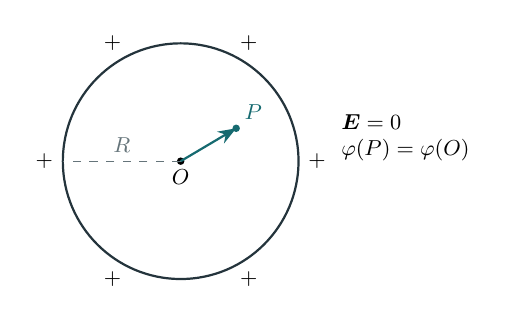
\begin{tikzpicture}[scale=.87,transform shape]
\draw[object](0,0)circle(1.72);\foreach \a in {0,60,...,300}{\node at (\a:1.99){$+$};}\fill(0,0)circle(1.55pt)node[below]{$O$};\fill[accent](.81,.48)circle(1.55pt)node[above right]{$P$};\draw[motion](0,0)--(.81,.48);\draw[guide](0,0)--(-1.72,0)node[midway,above]{$R$};\node[right,align=left]at(2.22,.34){$\vect E=0$\\$\varphi(P)=\varphi(O)$};
\end{tikzpicture}
\figcaption{变图 电1.4V1\quad 从球心移到偏心内点，电势沿途保持}
\end{minipage}\end{center}
\item 腔内置点电荷 $q$，导体本身的总电荷为 $Q$。变图电1.4V2的虚线球面位于金属中并包围空腔，故其电通量为零。由高斯定律和导体电荷守恒，
\[
q+Q_{\rm in}=0,\qquad
Q_{\rm in}+Q_{\rm out}=Q,\qquad
Q_{\rm out}=Q+q.
\]
偏心 $q$ 使内表面局部密度随位置改变。外部区域的边界仍是球形等势面，外部无外加场，故由外部问题的唯一性，外电荷在球面上均匀分布。
\begin{center}\begin{minipage}{.98\linewidth}\centering
\begin{tikzpicture}[scale=.87,transform shape]
\fill[accent!13](0,0)circle(1.78);\fill[white](0,0)circle(1.38);\draw[object](0,0)circle(1.78);\draw[object](0,0)circle(1.38);\draw[guide](0,0)circle(1.57);\fill[accent](.54,.27)circle(1.75pt)node[above right]{$q$};\node at(-.42,-.37){腔内};\draw[guide](-1.57,0)--(-2.40,0)node[left]{高斯面};\draw[guide](1.01,-.94)--(2.17,-1.14)node[right]{$Q_{\rm in}=-q$};\draw[guide](1.55,.88)--(2.19,1.27)node[right]{$Q_{\rm out}=Q+q$};
\end{tikzpicture}
\figcaption{变图 电1.4V2\quad 金属中的高斯面包围点电荷和内表面感应电荷}
\end{minipage}\end{center}
\item 令两面元的共同角因子为 $\mathcal C=k\sigma\dd\Omega/\cos\alpha$。对指数 $2+\delta$，由
\[
(\ell/s_i)^\delta=1+\delta\ln(\ell/s_i)+O(\delta^2)
\]
得到 $\dd E_{\rm pair}=\mathcal C\,\delta\ln(s_2/s_1)+O(\delta^2)$，一阶中尺度 $\ell$ 在两项的差内约去。变图电1.4V3取 $s_2=3s_1$、$\ell=2s_1$，比较完整的 $2^\delta-(2/3)^\delta$ 和一阶直线 $\delta\ln3$。
\begin{center}\begin{minipage}{.98\linewidth}\centering
\begin{tikzpicture}[scale=.87,transform shape]
\draw[axis](-2.92,1.72)--(3.35,1.72)node[right]{$\delta$};\draw[axis](0,.11)--(0,3.63)node[above]{$\dd E_{\rm pair}/\mathcal C$};\draw[traj,domain=-2.68:2.68,samples=72]plot(\x,{1.72+8*(pow(2,\x/16)-pow(2/3,\x/16))});\draw[guide,domain=-2.68:2.68,samples=72]plot(\x,{1.72+8*ln(3)*\x/16});\node[above left]at(2.40,3.12){完整差};\node[below right]at(-2.57,.35){一阶线};\node[left]at(0,1.72){0};
\end{tikzpicture}
\figcaption{变图 电1.4V3\quad 指数偏离零时，近、远场差的首项正比于距离比的对数}
\end{minipage}\end{center}
\item 若导体外另有点电荷，金属表面作为同一导体仍等势。变图电1.4V4取中性导体和右侧正电荷作示意，外表面上靠近它的一侧出现负感应电荷，远侧重新分配正电荷。空腔的内表面仍为同一常势，腔内无电荷。由拉普拉斯方程的极值原理，腔内电势处处等于这个常数，所以 $\vect E_{\rm cavity}=0$，屏蔽仍成立。
\begin{center}\begin{minipage}{.98\linewidth}\centering
\begin{tikzpicture}[scale=.87,transform shape]
\fill[accent!13](0,0)circle(1.78);\fill[white](0,0)circle(1.38);\draw[object](0,0)circle(1.78);\draw[object](0,0)circle(1.38);\fill[accent](3.22,.42)circle(1.8pt)node[above]{$q_{\rm ext}>0$};\foreach \a in {-38,0,34,63}{\node[warm]at(\a:1.98){$-$};}\foreach \a in {122,169,214,250}{\node[accent]at(\a:1.98){$+$};}\node[align=center]at(0,0){空腔\\$\vect E=0$};\draw[guide](1.0,-.96)--(2.18,-1.40)node[right]{内表面等势};
\end{tikzpicture}
\figcaption{变图 电1.4V4\quad 外部电荷改变外表面密度，空腔的等势条件仍成立}
\end{minipage}\end{center}
\item 变图电1.4V5左边的球心测点 $O$ 与每对对径面元等距，面积也相同。所以只要力沿连线、大小只随距离改变，两场便等大反向。右边改测偏心点 $P$，同一双锥的近、远两端面积按距离平方改变。反平方律使这两个因素对任意内点精确补偿。比较距离指数时应取偏心内点，或建立与之对应的内表面电荷响应。
\begin{center}\begin{minipage}{.98\linewidth}\centering
\begin{tikzpicture}[scale=.87,transform shape]
\draw[object](0,0)circle(1.54);\draw[guide](-1.54,0)--(1.54,0);\draw[force](0,.10)--(-.98,.10);\draw[force](0,-.10)--(.98,-.10);\fill(0,0)circle(1.5pt)node[below right]{$O$};\node[below]at(0,-1.70){球心：两距离相等};\begin{scope}[xshift=4.24cm]\draw[object](0,0)circle(1.54);\draw[guide](-1.54,0)--(1.54,0);\fill[accent](-.49,0)circle(1.5pt)node[below]{$P$};\draw[<->](-1.54,.27)--(-.49,.27)node[midway,above]{$s_1$};\draw[<->](-.49,.27)--(1.54,.27)node[midway,above]{$s_2$};\node[below]at(0,-1.70){偏心点：比较距离衰减};\end{scope}
\end{tikzpicture}
\figcaption{变图 电1.4V5\quad 球心的对径抵消与偏心内点的反平方抵消}
\end{minipage}\end{center}
\item 以球心为原点，球面元处的位置写为 $R\vect n$。对小位移 $\vect s$ 将
$ (\vect s-R\vect n)|\vect s-R\vect n|^{-3-\delta}$ 展至一阶，方向平均使用
$\langle n_i n_j\rangle=\delta_{ij}/3$，得
\[
\vect E(\vect s)
=-\frac{kQ}{3R^3}\delta(\ell/R)^\delta\vect s+O(s^3).
\]
变图电1.4V6取 $Q>0,\ell=R$，画 $\delta=\pm0.10$ 时的近心斜率。正指数偏差对应向心场，负偏差对应离心场；结果基于规定均匀的固定球面电荷。
\begin{center}\begin{minipage}{.98\linewidth}\centering
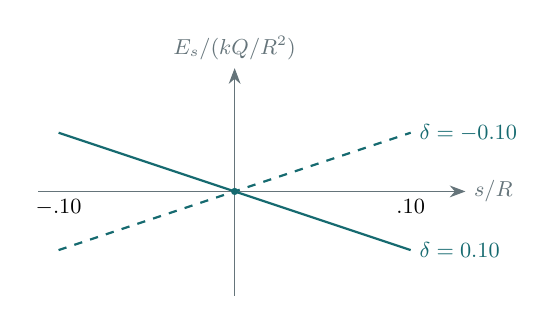
\begin{tikzpicture}[scale=.87,transform shape]
\draw[axis](-2.87,1.58)--(3.37,1.58)node[right]{$s/R$};\draw[axis](0,.06)--(0,3.38)node[above]{$E_s/(kQ/R^2)$};\draw[traj](-2.57,2.4367)--(2.57,.7233)node[right]{$\delta=0.10$};\draw[traj,dashed](-2.57,.7233)--(2.57,2.4367)node[right]{$\delta=-0.10$};\node[below]at(2.57,1.58){.10};\node[below]at(-2.57,1.58){$-.10$};\fill[accent](0,1.58)circle(1.5pt);
\end{tikzpicture}
\figcaption{变图 电1.4V6\quad 固定正电球面在两类指数偏差下给相反的近心斜率}
\end{minipage}\end{center}
\item 把均匀实心球分成同心薄壳，在内部半径 $s$ 处取测点。变图电1.4V7中，外于测点的薄壳对该点贡献为零；内于测点的薄壳对外部点的势等同于中心点电荷。内球所含电量为 $Q(s)=4\pi\rho s^3/3$，所以
\[
E_s=\frac{kQ(s)}{s^2}=\frac{\rho s}{3\varepsilon_0}.
\]
方向沿外径取正，随 $\rho$ 的符号改变。这个分层计算的内、外两项均使用反平方球壳结果。
\begin{center}\begin{minipage}{.98\linewidth}\centering
\begin{tikzpicture}[scale=.87,transform shape]
\fill[accent!16](0,0)circle(1.83);\fill[accent!38](0,0)circle(.96);\draw[object](0,0)circle(1.83);\draw[guide](0,0)circle(.96);\fill[accent](.96,0)circle(1.55pt)node[above]{$P$};\draw[<->](0,-.19)--(.96,-.19)node[midway,below]{$s$};\draw[force](1.10,.13)--(1.99,.13)node[right]{$E_s$};\draw[guide](-.71,-.61)--(-2.14,-1.35)node[left]{$Q(s)$};\draw[guide](1.37,-.89)--(2.36,-1.29)node[right]{外薄壳给零场};
\end{tikzpicture}
\figcaption{变图 电1.4V7\quad 实心球在内点的场只由该半径内的球壳贡献}
\end{minipage}\end{center}
\item 设两套平衡解的差势为 $w$。变图电1.4V8中对导体外区域 $\mathcal D$ 作格林恒等式，法向 $\vect n$ 指向区域外部。因 $\nabla^2 w=0$，
\[
\varepsilon_0\int_{\mathcal D}|\nabla w|^2\dd V
=\varepsilon_0\oint_{\partial\mathcal D}w\frac{\partial w}{\partial n}\dd S .
\]
无穷远项随边界外移趋零。若表面电势已给定，内圈上 $w=0$；若给定孤立导体总电荷，内圈上 $w=C$，积分为 $C\Delta Q=0$。两种设定都令差场为零，理由分别是常值的确定和积分通量的确定。
\begin{center}\begin{minipage}{.98\linewidth}\centering
\begin{tikzpicture}[scale=.87,transform shape]
\fill[accent!10](0,0)circle(2.05);\fill[gray!18](0,0)circle(.91);\draw[guide](0,0)circle(2.05);\draw[object](0,0)circle(.91);\node at(0,0){金属};\node at(-1.42,.51){$\mathcal D$};\draw[force](1.38,0)--(.98,0)node[above,midway]{$\vect n$};\draw[force](1.91,1.0)--(2.50,1.33)node[above]{$\vect n$};\node[right]at(2.45,1.92){远处截断面};\node[align=left,right]at(2.45,-.65){内边界：\\$w=0$ 或 $w=C$};
\end{tikzpicture}
\figcaption{变图 电1.4V8\quad 格林积分的内边界位于导体表面，外边界最后移向无穷远}
\end{minipage}\end{center}
\end{enumerate}

\clearpage

\pdfbookmark[2]{第 5 题 异号半圆环在轴线上的电场}{q5}

\section*{第 5 题\quad 异号半圆环在轴线上的电场}\label{q:5}

半径为$R$的圆环位于$xy$平面，圆心为原点。电荷线密度在$y<0$的半圆上为$+\lambda_0$，在$y>0$的半圆上为$-\lambda_0$，其中$\lambda_0>0$。求垂直于圆环平面、通过圆心的$z$轴上任意一点的电场。

\begin{center}\begin{minipage}{0.97\linewidth}\centering
\begin{tikzpicture}[x=1cm,y=1cm]
\draw[axis] (-2.4,0)--(2.5,0) node[right] {$x$};\draw[axis] (0,-2.2)--(0,2.3) node[above] {$y$};
\draw[very thick,warm] (-1.7,0) arc (180:360:1.7);\draw[very thick,accent] (1.7,0) arc (0:180:1.7);
\node at (0,-1.1) {$+\lambda_0$};\node at (0,1.1) {$-\lambda_0$};\node[below left] at (0,0) {$O$};
\draw[<->] (0,0)--({1.7/sqrt(2)},{-1.7/sqrt(2)}) node[midway,above] {$R$};\node[right,align=left] at (3,.2) {$z$轴垂直纸面\\观察点$P=(0,0,z)$};
\end{tikzpicture}\figcaption{图 电1.5　俯视圆环：下半环带正电，上半环带负电。}\end{minipage}\end{center}

\Needspace{5\baselineskip}

\pdfbookmark[3]{题型定位}{q5-h0}

\subsection*{题型定位}

几何轴线上的矢量叠加。半环带异号电荷，按两个反射分别消去两个分量，再积分留下的横向分量。

\Needspace{5\baselineskip}

\pdfbookmark[3]{知识点}{q5-h1}

\subsection*{知识点}

电荷元 $\dd q=\lambda R\dd\phi$，所有元距轴点 $P$ 都为 $d=\sqrt{R^2+z^2}$。$x$ 反射使 $E_x$ 消去，$y$ 反射同时翻转电荷符号使 $E_z$ 消去。电势沿轴为零，电场的横向分量由轴旁梯度给出。


\Needspace{5\baselineskip}

\pdfbookmark[3]{物理图像}{q5-h2}

\subsection*{物理图像}

图电1.5上半环负、下半环正。解图电1.5A画出 $x=0$ 的一正一负对，两个轴向分量相消，水平分量都指向 $+y$。解图电1.5B按 $z/R$ 表示场强，曲线在环心最高、离开两侧都下降。

\Needspace{5\baselineskip}

\pdfbookmark[3]{解题入口}{q5-h3}

\subsection*{解题入口}

把库仑场写成带符号的线积分，提取共同的 $d^{-3}$，按分量作三项角积分。也可先把正半环的每个元投影到环面，再向 $y$ 轴投影，最后将该分量加倍。

\Needspace{5\baselineskip}

\pdfbookmark[3]{标准解法}{q5-h4}

\subsection*{标准解法}

观察点取$P=(0,0,z)$。圆环所在的几何轴是 $z$ 轴。上、下半环线密度异号，沿图中的反射配对决定合场方向。
\begin{center}\begin{minipage}{0.97\linewidth}\centering
\begin{tikzpicture}[x=1cm,y=1cm]
\draw[axis] (-2.6,0)--(2.8,0) node[right] {$y$};\draw[axis] (0,-.3)--(0,3) node[above] {$z$};
\coordinate (P) at (0,1.8);\fill (P) circle (1.5pt) node[left] {$P$};
\fill[warm] (-1.6,0) circle (2pt) node[below] {$+\dd q$};\fill[accent] (1.6,0) circle (2pt) node[below] {$-\dd q$};
\draw[guide] (-1.6,0)--(P)--(1.6,0);\draw[force] (P)--(.8,2.7) node[right] {$\dd\vect E_+$};
\draw[motion] (P)--(.8,.9) node[right] {$\dd\vect E_-$};\draw[very thick,->] (P)--(1.6,1.8) node[right] {$\dd\vect E$};
\node at (0,-.8) {图示一对$x=0$的对称元；一般元再配$x\leftrightarrow-x$};
\end{tikzpicture}\figcaption{解图 电1.5A　正、负电荷的轴向分量抵消，y分量相加；横向分量须另由x对称配对消去。}\end{minipage}\end{center}
先按解图电1.5A配对：关于$x$轴对称的正、负电荷元对$P$等距，电荷大小相等，其$z$分量抵消、$y$分量同向；再用$x\leftrightarrow-x$的对称元消去$x$分量。于是总场只能沿$+y$方向。

取环上位置$\vect r'=(R\cos\phi,R\sin\phi,0)$，$\dd q=\lambda(\phi)R\dd\phi$，所有电荷元到$P$的距离相同：$d=\sqrt{R^2+z^2}$。有
\[\dd\vect E=\frac{k\lambda(\phi)R\dd\phi}{d^3}
(-R\cos\phi,-R\sin\phi,z).\]
其中$0<\phi<\pi$时$\lambda=-\lambda_0$，$\pi<\phi<2\pi$时$\lambda=+\lambda_0$。逐分量积分，
\begin{align*}
E_x&=-\frac{kR^2}{d^3}\int_0^{2\pi}\lambda(\phi)\cos\phi\,\dd\phi=0,\\
E_z&=\frac{kRz}{d^3}\left(-\lambda_0\pi+\lambda_0\pi\right)=0,\\
E_y&=-\frac{kR^2}{d^3}\left[-\lambda_0\int_0^\pi\sin\phi\,\dd\phi
+\lambda_0\int_\pi^{2\pi}\sin\phi\,\dd\phi\right]\\
&=\frac{4k\lambda_0R^2}{(R^2+z^2)^{3/2}}.
\end{align*}
\Needspace{4\baselineskip}
因此，轴上总场为
\result{\vect E(0,0,z)=\frac{\lambda_0R^2}{\pi\varepsilon_0(R^2+z^2)^{3/2}}\vect e_y.}
在$z=0$处，两半圆环各贡献$2k\lambda_0/R$，方向均从带正电的下半环指向带负电的上半环。结果对$z$为偶函数，因此在圆环上下两侧方向相同。

在远处，把圆环看成以偶极矩为首项的分布。总电荷为零，而电偶极矩为
\[\vect p=\int\vect r'\,\dd q=-4\lambda_0R^2\vect e_y.\]
$z$轴是该偶极矩的赤道方向，远处有$\vect E\simeq-k\vect p/|z|^3$，与上式的$|z|\gg R$极限相符。
\subsubsection*{半圆分量的逐次投影与轴上场强曲线}
还可只取正半圆计算，再利用正、负配对把y分量乘2。
在下半圆用$\theta\in[0,\pi]$记从负x端到正x端的角参数，
电荷元位置为$(-R\cos\theta,-R\sin\theta,0)$。
对$z>0$，面元到P的连线与z轴夹角为$\alpha$，有$\sin\alpha=R/d$。
先投影到环面、再投影到y轴，得到
\[
\dd E=\frac{k\lambda_0R\dd\theta}{d^2},\quad
\dd E_{xy}=\dd E\frac Rd,\quad
\dd E_y=\dd E_{xy}\sin\theta
=\frac{k\lambda_0R^2}{d^3}\sin\theta\dd\theta.
\]
因$d=\sqrt{R^2+z^2}$与积分角无关，正半环的贡献为
\[
E_{y,+}=\frac{k\lambda_0R^2}{d^3}\int_0^\pi\sin\theta\dd\theta
=\frac{2k\lambda_0R^2}{d^3},\qquad E_y=2E_{y,+}.
\]
这与前面的有符号矢量积分相同。对$z<0$虽轴向分量反转，
正负两元的轴向分量仍抵消，横向场仍沿$+y$。

\begin{center}\begin{minipage}{.97\linewidth}\centering
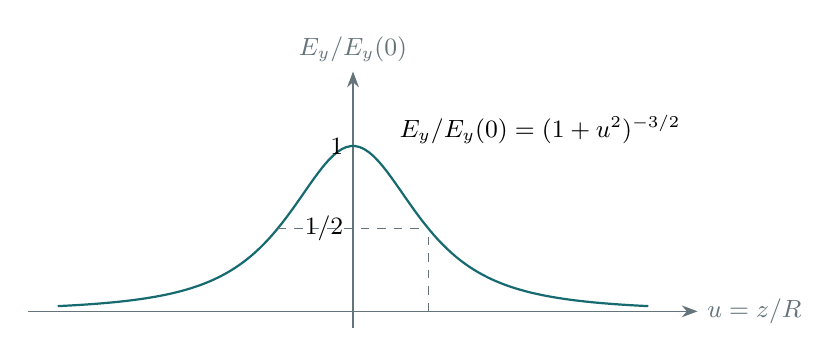
\begin{tikzpicture}[x=1.25cm,y=2.1cm,font=\small]
\draw[axis] (-3.3,0)--(3.5,0) node[right] {$u=z/R$};
\draw[axis] (0,-.1)--(0,1.45) node[above] {$E_y/E_y(0)$};
\draw[traj,domain=-3:3,samples=130] plot(\x,{pow(1+\x*\x,-1.5)});
\draw[guide] (-.76642094,.5)--(.76642094,.5);
\draw[guide] (.76642094,0)--(.76642094,.5);
\node[left] at (0,1) {$1$};\node[left] at (0,.5) {$1/2$};
\node at (1.9,1.1) {$E_y/E_y(0)=(1+u^2)^{-3/2}$};
\end{tikzpicture}
\figcaption{解图 电1.5B　环心场最大；两侧半高位置满足$|z|/R=\sqrt{2^{2/3}-1}$。}
\end{minipage}\end{center}
解图电1.5B的曲线关于 $z=0$ 偶对称，上、下两侧场都沿 $+y$。
近环心有$E_y/E_y(0)=1-3z^2/(2R^2)+O(z^4/R^4)$，
远处则有
\[
\vect E=\frac{4k\lambda_0R^2}{|z|^3}
\left[1-\frac{3R^2}{2z^2}+O(R^4/z^4)\right]\vect e_y.
\]
总电荷为零使单极项消失，前面从偶极矩所得的是首个 $|z|^{-3}$ 项，
更高修正相对它为$O(R^2/z^2)$。

\subsubsection*{零电势轴与非零横向梯度}
轴上所有电荷元等距，所以$\varphi(0,0,z)=k\int\dd q/d=0$。
沿轴求导得到 $E_z=0$，横向的电场由轴旁电势的变化给出。
令$f(z)=4k\lambda_0R^2(R^2+z^2)^{-3/2}$，
在轴旁的小横向位移y处，势的首项为
\[
\varphi(0,y,z)=-f(z)y+O(y^3),\quad
E_y(0,y,z)=f(z)+O(y^2),\quad
E_z(0,y,z)=f'(z)y+O(y^3).
\]
势对y为奇函数，因为$y\to-y$同时交换正负电荷半环。
沿轴取 $y=0$，势恒为零，故沿轴求导得到 $E_z=0$。横向的势梯度由 $-f(z)y$ 给出，在轴上取 $\partial\varphi/\partial y=-f(z)$。轴旁的一阶 $E_z$ 则给 $\partial E_z/\partial y=\partial E_y/\partial z=f'(z)$（取在轴上）。
解图电1.5A中的合场正对应这个横向梯度。


\Needspace{5\baselineskip}

\pdfbookmark[3]{关键洞察}{q5-h5}

\subsection*{关键洞察}

正、负半环的总电荷相消，偶极矩沿 $-y$。$z$ 轴位于偶极赤道方向，远处场沿 $+y$ 并按 $|z|^{-3}$ 衰减。轴上零势在轴旁按 $-E_y(z)y$ 变化，因此沿 $y$ 仍有合场。

\Needspace{5\baselineskip}

\pdfbookmark[3]{易错点}{q5-h6}

\subsection*{易错点}

轴线上的距离相同，电荷符号和各场分量仍要分别写出。负线密度已经包含吸引方向。配 $x$ 反射消左右分量，配异号的 $y$ 反射消法向分量，再作投影积分。判断电势斜率时，沿轴和横向取的是不同导数。

\Needspace{5\baselineskip}

\pdfbookmark[3]{课堂讲解建议}{q5-h7}

\subsection*{课堂讲解建议}

先在图电1.5选一个一般元，再让学生指出两次反射分别将它送到何处。按解图电1.5A画成两个三角形，比较各轴分量的符号。两组分别用带符号积分和两次投影求同一 $d^{-3}$ 系数。

读解图电1.5B的环心附近和半高位置，再用变图电1.5V5画一条穿过零势轴的横线，沿这条线解释为什么场为正 $y$ 向。最后用变图电1.5V8比较不同线密度中对轴上场有效的角谐波。

\Needspace{5\baselineskip}

\pdfbookmark[3]{变式训练}{q5-h8}

\subsection*{变式训练}

\begin{enumerate}
\item 轴上归一场为 $f(u)=(1+u^2)^{-3/2}$，其中 $u=z/R$。变图电1.5V1的纵轴取它的导数
\[
f'(u)=-\frac{3u}{(1+u^2)^{5/2}}.
\]
曲线在两侧分别为正和负，所以 $z=0$ 是最大点，$E(0)=4k\lambda_0/R$。向两侧远离环心，场强都随 $|z|$ 下降。
\begin{center}\begin{minipage}{.98\linewidth}\centering
\begin{tikzpicture}[scale=.87,transform shape]
\draw[axis](-3.03,1.75)--(3.38,1.75)node[right]{$u$};\draw[axis](0,.12)--(0,3.87)node[above]{$f^\prime(u)$};\draw[traj,domain=-2.95:2.95,samples=72]plot(\x,{1.75-1.85*3*(\x/2)/pow(1+(\x/2)^2,2.5)});\node[above left]at(-1.68,3.09){场强递增};\node[below right]at(1.41,.33){场强递减};\fill[accent](0,1.75)circle(1.5pt);
\end{tikzpicture}
\figcaption{变图 电1.5V1\quad 导数的正负变化给出环心处的最大值}
\end{minipage}\end{center}
\item 求场强为环心一半的位置，写成 $(1+z^2/R^2)^{3/2}=2$，故
\[
z=\pm R\sqrt{2^{2/3}-1}.
\]
变图电1.5V2用半高水平线截归一场曲线，对称的两点分别在约 $\pm0.7664R$，各自的场方向仍为 $+y$。
\begin{center}\begin{minipage}{.98\linewidth}\centering
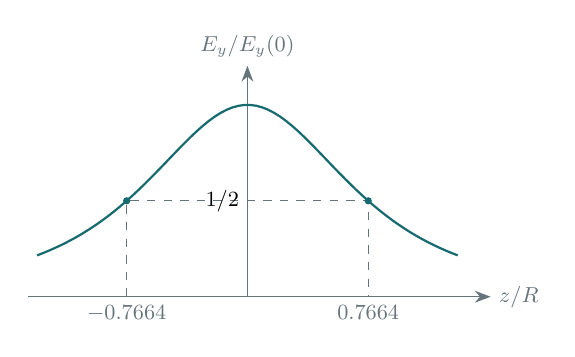
\begin{tikzpicture}[scale=.87,transform shape]
\draw[axis](-3.2,0)--(3.55,0)node[right]{$z/R$};\draw[axis](0,0)--(0,3.37)node[above]{$E_y/E_y(0)$};\draw[traj,domain=-3.07:3.07,samples=72]plot(\x,{2.8*pow(1+(\x/2.3)^2,-1.5)});\draw[guide](-1.7627681540440234,0)node[below]{$-0.7664$}--(-1.7627681540440234,1.4)--(1.7627681540440234,1.4)--(1.7627681540440234,0)node[below]{$0.7664$};\node[left]at(0,1.4){$1/2$};\fill[accent](1.7627681540440234,1.4)circle(1.51pt);\fill[accent](-1.7627681540440234,1.4)circle(1.51pt);
\end{tikzpicture}
\figcaption{变图 电1.5V2\quad 半高线与偶函数曲线相交于轴的两侧}
\end{minipage}\end{center}
\item 另叠加均匀线密度 $\lambda_c$ 时，均匀部分的横向分量相消，只增加
\[
E_z=\frac{2\pi k\lambda_c R z}{(R^2+z^2)^{3/2}}.
\]
变图电1.5V3取 $\lambda_c=2\lambda_0/\pi$，此时 $E_z/E_y=z/R$。在 $z=+R$、$-R$ 处，新增分量分别为等大向上、向下，合场与 $+y$ 方向分别成 $45^\circ$ 与 $-45^\circ$。$y$ 分量来自原异号分布。
\begin{center}\begin{minipage}{.98\linewidth}\centering
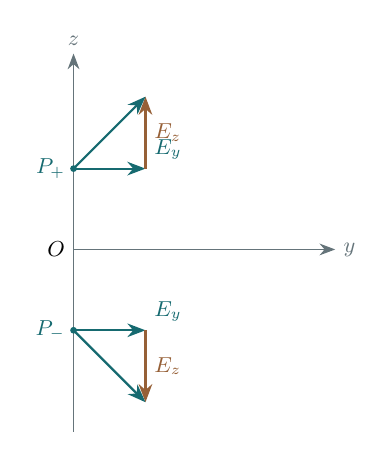
\begin{tikzpicture}[scale=.87,transform shape]
\draw[axis](0,-2.66)--(0,2.86)node[above]{$z$};\draw[axis](0,0)--(3.82,0)node[right]{$y$};\foreach \ys/\sg/\lab in {1.18/1/$P_+$,-1.18/-1/$P_-$}{\fill[accent](0,\ys)circle(1.4pt)node[left]{\lab};\draw[motion](0,\ys)--(1.05,\ys)node[above right]{$E_y$};\draw[force](1.05,\ys)--(1.05,{\ys+1.05*\sg})node[right,midway]{$E_z$};\draw[traj,-{Stealth}](0,\ys)--(1.05,{\ys+1.05*\sg});}\node[left]at(0,0){$O$};
\end{tikzpicture}
\figcaption{变图 电1.5V3\quad 异号半环与均匀附加电荷产生相互垂直的分量}
\end{minipage}\end{center}
\item 线密度改为 $\lambda(\phi)=\lambda_1\sin\phi$，以 $\lambda_1>0$ 作图。把它代入矢量积分，$x$、$z$ 分量含的 $\int\sin\phi\cos\phi\,\dd\phi$ 和 $\int\sin\phi\,\dd\phi$ 均为零。$y$ 分量含 $\int_0^{2\pi}\sin^2\phi\,\dd\phi=\pi$，故
\[
\vect E=-\frac{\pi k\lambda_1R^2}{(R^2+z^2)^{3/2}}\vect e_y .
\]
变图电1.5V4的第一半周 $\sin\phi>0$，对应上半环带正电，合场朝向下半环。
\begin{center}\begin{minipage}{.98\linewidth}\centering
\begin{tikzpicture}[scale=.87,transform shape]
\draw[axis](0,1.68)--(6.12,1.68)node[right]{$\phi$};\draw[axis](0,.03)--(0,3.48)node[above]{$\lambda/\lambda_1$};\draw[traj,domain=0:5.65,samples=72]plot(\x,{1.68+1.42*sin(360*\x/5.65)});\node[below right]at(2.825,1.68){$\pi$};\node[below right]at(5.65,1.68){$2\pi$};\node[above]at(1.43,3.10){上半环};\node[below]at(4.26,.26){下半环};
\end{tikzpicture}
\figcaption{变图 电1.5V4\quad 正弦线密度取正的角区间对应上半环}
\end{minipage}\end{center}
\item 轴上每个电荷元与测点等距，且总电荷为零，因此 $\varphi(0,0,z)=0$。变图电1.5V5固定 $z$，沿 $y$ 穿过轴线。小 $y$ 时有
\[
\varphi(0,y,z)=-E_y(z)y+O(y^3),
\]
曲线在交点的斜率为 $-E_y(z)$；沿垂直纸面的 $z$ 轴走时，势值一直是零，给出 $E_z=0$。同一点的两个方向导数不同。
\begin{center}\begin{minipage}{.98\linewidth}\centering
\begin{tikzpicture}[scale=.87,transform shape]
\draw[axis](-2.78,1.75)--(3.32,1.75)node[right]{$y$};\draw[axis](0,.03)--(0,3.52)node[above]{$\varphi$};\draw[traj](-2.64,3.11)--(2.64,.39);\fill[accent](0,1.75)circle(1.5pt)node[above right]{轴上点};\draw[force](.27,.76)--(1.66,.76)node[right]{$\vect E$};\node at(-1.52,.4){固定 $z$};
\end{tikzpicture}
\figcaption{变图 电1.5V5\quad 零势轴横向的势梯度与非零横向电场相对应}
\end{minipage}\end{center}
\item 在 $|z|\gg R$ 时，令 $w=R^2/z^2$，将轴场与偶极首项 $E_{\rm dip}=4k\lambda_0R^2/|z|^3$ 作比，
\[
\frac{E_y}{E_{\rm dip}}
=(1+w)^{-3/2}=1-\frac32w+O(w^2).
\]
变图电1.5V6画出准确比值及保留首修正的直线。以 $|z|=3R$ 为例，二者分别约为0.8538和0.8333。单极项因总电荷为零而消失，首相对修正为 $O(R^2/z^2)$。
\begin{center}\begin{minipage}{.98\linewidth}\centering
\begin{tikzpicture}[scale=.87,transform shape]
\draw[axis](0,0)--(6.12,0)node[right]{$w=R^2/z^2$};\draw[axis](0,0)--(0,3.12)node[above]{$E_y/E_{\rm dip}$};\draw[traj,domain=0:5.4,samples=72]plot(\x,{5*(pow(1+\x/16,-1.5)-.5)});\draw[guide,domain=0:5.30,samples=72]plot(\x,{5*(.5-1.5*\x/16)});\draw[guide](1.7778,0)node[below]{$1/9$}--(1.7778,1.76907);\fill[accent](1.7778,1.76907)circle(1.5pt);\node[left]at(0,2.5){1};\node[above right]at(4.02,1.07){准确比值};\node[right]at(4.18,.50){首修正};
\end{tikzpicture}
\figcaption{变图 电1.5V6\quad 偶极首项略大于准确轴场，首个相对修正为负}
\end{minipage}\end{center}
\item 在 $z=\pm R$ 两点代入 $d=\sqrt2R$，得
\[
E_y(+R)=E_y(-R)=\frac{E_y(0)}{2\sqrt2}.
\]
变图电1.5V7的三个场箭头共用一套长度标尺，两侧各是环心箭头的 $1/(2\sqrt2)$，方向都为 $+y$。它们各自的轴向分量已由正负半环配对抵消。
\begin{center}\begin{minipage}{.98\linewidth}\centering
\begin{tikzpicture}[scale=.87,transform shape]
\draw[axis](0,-1.87)--(0,2.34)node[above]{$z$};\draw[axis](-.26,0)--(4.2,0)node[right]{$y$};\foreach \z/\lab in {1.27/$R$,-1.27/$-R$}{\fill[accent](0,\z)circle(1.4pt)node[left]{\lab};\draw[motion](0,\z)--(1.16673,\z)node[right]{$E_y(0)/(2\sqrt2)$};}\draw[motion](0,0)--(3.3,0)node[midway,above]{$E_y(0)$};
\end{tikzpicture}
\figcaption{变图 电1.5V7\quad 等高的上下两点得到相等、同向的横场}
\end{minipage}\end{center}
\item 对一般 $\lambda(\phi)$，把库仑积分分成
\[
E_x=-\frac{kR^2}{d^3}\int_0^{2\pi}\lambda\cos\phi\,\dd\phi,\quad
E_y=-\frac{kR^2}{d^3}\int_0^{2\pi}\lambda\sin\phi\,\dd\phi,\quad
E_z=\frac{kRz}{d^3}\int_0^{2\pi}\lambda\,\dd\phi .
\]
三式分别读取第一余弦谐波、第一正弦谐波及平均值。变图电1.5V8给两条线密度曲线，虚线是在 $\sin\phi$ 上新增 $0.45\sin3\phi$ 后的结果；三次谐波与上述三种权函数都正交，轴场保持。离轴后各元距离一般随角度改变，高阶谐波也可贡献电场。
\begin{center}\begin{minipage}{.98\linewidth}\centering
\begin{tikzpicture}[scale=.87,transform shape]
\draw[axis](0,1.75)--(6.16,1.75)node[right]{$\phi$};\draw[axis](0,.02)--(0,3.58)node[above]{$\lambda/\lambda_1$};\draw[traj,domain=0:5.75,samples=72]plot(\x,{1.75+1.19*sin(360*\x/5.75)});\draw[traj,dashed,domain=0:5.75,samples=72]plot(\x,{1.75+1.19*(sin(360*\x/5.75)+.45*sin(1080*\x/5.75))});\node[below]at(2.875,1.75){$\pi$};\node[below]at(5.75,1.75){$2\pi$};\node[right]at(4.47,3.14){实线：$\sin\phi$};\node[right]at(4.47,2.72){虚线：加三次谐波};
\end{tikzpicture}
\figcaption{变图 电1.5V8\quad 增加三次角谐波会改变环上密度，轴上三种投影保持}
\end{minipage}\end{center}
\end{enumerate}

\clearpage

\pdfbookmark[2]{第 6 题 半圆弧与两条半无限直线的电场}{q6}

\section*{第 6 题\quad 半圆弧与两条半无限直线的电场}\label{q:6}

一条均匀带电细线弯成图示形状：左侧$AB$为半圆弧；$AA'$和$BB'$为分别与圆弧相切、向右无限延伸的两条平行直线。求半圆圆心$O$处的电场。可自设圆弧半径$R$和电荷线密度$\lambda$。

\begin{center}\begin{minipage}{0.97\linewidth}\centering
\begin{tikzpicture}[x=1cm,y=1cm]\draw[object] (0,1.5) arc (90:270:1.5);\draw[object,->] (0,1.5)--(4,1.5);\draw[object,->] (0,-1.5)--(4,-1.5);\draw[guide] (0,-1.5)--(0,1.5);\fill (0,0) circle (1.2pt) node[right] {$O$};\node[above] at (0,1.5) {$A$};\node[below] at (0,-1.5) {$B$};\node[above] at (3.7,1.5) {$A'$};\node[below] at (3.7,-1.5) {$B'$};\end{tikzpicture}\figcaption{图 电1.6　两条直线从圆弧端点向右无限延伸，线密度处处相同。}\end{minipage}\end{center}

\Needspace{5\baselineskip}

\pdfbookmark[3]{题型定位}{q6-h0}

\subsection*{题型定位}

由半圆弧和两条切线组成的连续电荷分布。先用同张角线元配对，再用分段积分求同一零场，并讨论有限长度和微扰。

\Needspace{5\baselineskip}

\pdfbookmark[3]{知识点}{q6-h1}

\subsection*{知识点}

弧元 $\dd l_1=R\dd\phi$，切线元 $\dd l_2=R\sec^2\phi\,\dd\phi$；后者距 $O$ 为 $R\sec\phi$，二者的比值 $\dd l/r^2$ 相同。上下镜面对称只消去竖直分量。场积分与以无穷远为零的势积分具有不同的远端收敛性。


\Needspace{5\baselineskip}

\pdfbookmark[3]{物理图像}{q6-h2}

\subsection*{物理图像}

解图电1.6A把左上弧元与右下直线元配对，两个场方向相反。左下弧元配上方直线元。解图电1.6B显示，两直线有限时没有完全补上左弧的向右场，残余场随长度增大逐渐趋零。

\Needspace{5\baselineskip}

\pdfbookmark[3]{解题入口}{q6-h3}

\subsection*{解题入口}

以 $O$ 为射线极点，令 $\phi$ 为其与向下竖直线的夹角。由 $x=R\tan\phi$ 换元，或取垂直射线的线元投影，得到切线元长度与半圆元共享同一角变量。随后分段求上、下两直线的各轴场。

\Needspace{5\baselineskip}

\pdfbookmark[3]{标准解法}{q6-h4}

\subsection*{标准解法}

设$\lambda>0$，最后的矢量结论同样适用于负线密度。解图电1.6A中上、下直线关于水平轴对称，其竖直场分量相消；左半圆弧在$O$的合场向右，两条直线在$O$的合场向左。需要比较两者大小。
\begin{center}\begin{minipage}{0.97\linewidth}\centering
\begin{tikzpicture}[x=1cm,y=1cm]\draw[object] (0,1.5) arc (90:270:1.5);\draw[object,->] (0,1.5)--(4,1.5);\draw[object,->] (0,-1.5)--(4,-1.5);\draw[guide] (0,-1.5)--(0,1.5);\fill (0,0) circle (1.2pt) node[right] {$O$};\node[above] at (0,1.5) {$A$};\node[below] at (0,-1.5) {$B$};\node[above] at (3.7,1.5) {$A'$};\node[below] at (3.7,-1.5) {$B'$};
\draw[guide] ({-1.5/sqrt(2)},{1.5/sqrt(2)})--(1.5,-1.5);\fill[accent] ({-1.5/sqrt(2)},{1.5/sqrt(2)}) circle (2pt) node[left] {$\dd l_1$};\fill[accent] (1.5,-1.5) circle (2pt) node[below right] {$\dd l_2$};
\draw[force] (0,0)--(.7,-.7);\draw[motion] (0,0)--(-.7,.7);
\draw (0,-.55) arc (-90:-45:.55);\node at (.28,-.65) {$\phi$};\node at (2.5,.4) {$r=R/\cos\phi$};\node at (2.5,-.2) {$\dd l_2=R\sec^2\phi\,\dd\phi$};
\end{tikzpicture}\figcaption{解图 电1.6A　左上四分之一弧与下方直线逐元配对；反向场元恰好等大。}\end{minipage}\end{center}
先保留逐元配对法。取左上四分之一弧上一段$\dd l_1$，其到$O$的连线延长后交下方直线于$\dd l_2$。令连线与向下竖直方向夹角为$\phi$，则
\[\dd l_1=R\dd\phi,\qquad r=\frac R{\cos\phi},\qquad
x=R\tan\phi,\qquad \dd l_2=R\sec^2\phi\,\dd\phi.\]
两段电荷产生的电场大小为
\[\dd E_1=\frac{k\lambda\dd l_1}{R^2}=\frac{k\lambda}{R}\dd\phi,\qquad
\dd E_2=\frac{k\lambda\dd l_2}{r^2}=\frac{k\lambda}{R}\dd\phi.\]
两个电荷元位于$O$两侧同一直线上，电场方向相反，所以逐对抵消。当$0\le\phi<\pi/2$时，左上四分之一弧与整个下方半无限直线一一对应；左下四分之一弧同样与上方直线配对。由此得到
\result{\vect E(O)=\vect0.}

也可逐段积分，分别求出三部分的场。左半圆弧的水平场为
\[E_{{\rm arc},x}=-\frac{k\lambda}{R}\int_{\pi/2}^{3\pi/2}\cos\theta\,\dd\theta
=\frac{2k\lambda}{R}.\]
上方直线电荷元$(x,R)$在$O$的场为
\[\dd\vect E_{\rm top}=-k\lambda\frac{x\vect e_x+R\vect e_y}{(x^2+R^2)^{3/2}}\dd x.\]
利用
\[\int_0^\infty\frac{x\dd x}{(x^2+R^2)^{3/2}}=\frac1R,\qquad
\int_0^\infty\frac{R\dd x}{(x^2+R^2)^{3/2}}=\frac1R,\]
得$\vect E_{\rm top}=-(k\lambda/R)(\vect e_x+\vect e_y)$。下方直线给出
$\vect E_{\rm bottom}=-(k\lambda/R)(\vect e_x-\vect e_y)$，三部分相加确为零。

上下对称消去竖直分量；半圆与两条同密度半无限切线的场则在水平方向恰好相消。截短直线后的剩余场见下文。
\subsubsection*{线元投影、无穷端点与配对的适用条件}
解图电1.6A中，将下直线元$\dd l_2$投影到垂直于OP的方向，记投影长度为$\dd l_2'$。
同一小张角给$\dd l_2'=r\dd\phi$，而投影关系给
\[
\dd l_2'=\dd l_2\cos\phi,\qquad
\cos\phi=\frac Rr,\qquad
\frac{\dd l_2}{r^2}=\frac{\dd\phi}{r\cos\phi}=\frac{\dd\phi}R.
\]
这与$x=R\tan\phi$的导数计算是同一几何关系。
同张角下，直线元较长，这个长度因子恰与更大的距离平方相消。
当$\phi\to\pi/2$，对应点$x\to\infty$，
配对应理解为有限角区间逐渐逼近端点的反常积分极限。
单条直线的场积分因被积函数按$x^{-2}$或更快衰减而收敛，
所以取这一极限不会留下额外的端点场。

镜面对称给 $E_y(O)=0$，各段场的水平部分由前面的配对或分段积分得到。

若两条直线都在长度L处截断，水平合场的完整计算为
\[
\begin{aligned}
E_{{\rm lines},x}
&=-2k\lambda\int_0^L\frac{x\dd x}{(x^2+R^2)^{3/2}}\\
&=-2k\lambda\left(\frac1R-\frac1{\sqrt{R^2+L^2}}\right),\\
E_x(O)&=\frac{2k\lambda}{\sqrt{R^2+L^2}}.
\end{aligned}
\]
解图电1.6B按正线密度归一；长度增加时残余场向右且逐渐减小，
按 $2k\lambda/L$ 的尺度减小并在半无限极限趋零。

\begin{center}\begin{minipage}{.97\linewidth}\centering
\begin{tikzpicture}[x=1.6cm,y=2.1cm,font=\small]
\draw[axis] (0,0)--(4.7,0) node[right] {$u=L/R$};
\draw[axis] (0,-.1)--(0,1.4) node[above] {$E_x/(2k\lambda/R)$};
\draw[traj,domain=0:4.3,samples=100] plot(\x,{1/sqrt(1+\x*\x)});
\node[left] at (0,1) {$1$};\node at (2.7,1.05) {$(1+u^2)^{-1/2}$};
\draw[guide] (1,0) node[below] {$1$}--(1,.707106781);
\node[right] at (1,.707106781) {$1/\sqrt2$};
\end{tikzpicture}
\figcaption{解图 电1.6B　两直线截短后的环心残余场；纵轴按$\lambda>0$归一。}
\end{minipage}\end{center}

\subsubsection*{零场点附近是否稳定}
考察离开 $O$ 一小段后的运动，需要求该处电场的一阶变化。
按解图电1.6A，以两条切线的延伸方向为 $+x$、由下切线指向上切线为 $+y$，取 $z$ 垂直于这两条直线和半圆所在的平面，
在O附近对库仑场求一阶导数：每个电荷元贡献
\[
J_{ij}=k\int\frac{\dd q}{r'^3}(\delta_{ij}-3n_i n_j),
\qquad\vect n=\vect r'/r',\quad\vect E(\vect r)=J\vect r+O(|\vect r|^2).
\]
半圆弧给$J_{\rm arc}=(k\lambda/R^2)\operatorname{diag}(-\pi/2,-\pi/2,\pi)$。
两条直线的x导数积分为
$2k\lambda\int_0^\infty(R^2-2x^2)(x^2+R^2)^{-5/2}\dd x=0$，
y、z导数分别为$-2k\lambda/R^2$和$2k\lambda/R^2$，交叉项由对称性消去。
故
\[
J=\frac{k\lambda}{R^2}\operatorname{diag}\left(-\frac\pi2,-\frac\pi2-2,\pi+2\right),
\qquad\operatorname{tr}J=0.
\]
若$\lambda>0$、试探电荷为正且受到平面约束，两个允许方向都有一阶回复力；
若允许三维位移，法向电场随法向偏离同向增长，因而出现失稳。


\Needspace{5\baselineskip}

\pdfbookmark[3]{关键洞察}{q6-h5}

\subsection*{关键洞察}

直线元随角度增大的长度因子与反平方距离因子恰好相消。原点零场给平衡；对正试探电荷，平面内两个方向的一阶电场均指回中心，面外电场指向离开的方向。

\Needspace{5\baselineskip}

\pdfbookmark[3]{易错点}{q6-h6}

\subsection*{易错点}

同张角给相同的角变量，弧元和直线元仍有不同长度。上直线场朝左下，下直线场朝左上，求各自矢量后再相加。从 $\phi\to\pi/2$ 到直线无穷远是反常积分极限；讨论势时可以采用有限点的势差。

\Needspace{5\baselineskip}

\pdfbookmark[3]{课堂讲解建议}{q6-h7}

\subsection*{课堂讲解建议}

先在解图电1.6A旁分别画出每段电荷在 $O$ 的合场方向。让一组求 $x=R\tan\phi$ 的导数，另一组由变图电1.6V5画垂直投影，随后用共同的 $\dd l/r^2$ 联系两种写法。

把两直线截成 $L$，比较解图电1.6B不同长度的残余场，再用变图电1.6V6读取给定精度的最短直线。讨论去掉一条直线后，分别保留哪个水平和竖直分量。

\Needspace{5\baselineskip}

\pdfbookmark[3]{变式训练}{q6-h8}

\subsection*{变式训练}

\begin{enumerate}
\item 若圆弧线密度为 $\lambda_a$，两切线均为 $\lambda_l$，弧的合场为 $2k\lambda_a\vect e_x/R$，切线的合场为 $-2k\lambda_l\vect e_x/R$。因此
\[
\vect E=\frac{2k}{R}(\lambda_a-\lambda_l)\vect e_x.
\]
变图电1.6V1示意两种线密度均为正且 $\lambda_a>\lambda_l$ 的情形，向右弧场大于两切线向左场，合场朝右。反过来 $\lambda_a<\lambda_l$ 时水平分量改号。
\begin{center}\begin{minipage}{.98\linewidth}\centering
\begin{tikzpicture}[scale=.87,transform shape]
\draw[object](0,1.32)arc (90:270:1.32);\draw[object](0,1.32)--(3.84,1.32);\draw[object](0,-1.32)--(3.84,-1.32);\fill (0,0)circle(1.4pt)node[left]{$O$};\node[left]at(-1.42,0){$\lambda_a$};\node[above]at(2.65,1.32){$\lambda_l$};\node[below]at(2.65,-1.32){$\lambda_l$};\draw[force](0,.62)--(2.42,.62)node[midway,above]{$\vect E_a$};\draw[motion](0,-.57)--(-1.54,-.57)node[midway,below]{$\vect E_l$};\draw[traj,-{Stealth}](0,0)--(.88,0)node[right]{$\vect E$};\draw[motion](3.84,1.32)--(4.24,1.32);\draw[motion](3.84,-1.32)--(4.24,-1.32);
\end{tikzpicture}
\figcaption{变图 电1.6V1\quad 两切线的竖直分量仍相消，密度差留下水平场}
\end{minipage}\end{center}
\item 两条切线从端点起各截到 $x=L$。变图电1.6V2把截去的远尾画成虚线，有限直线的水平场为
\[
-2k\lambda\left(\frac1R-\frac{1}{\sqrt{R^2+L^2}}\right).
\]
加上半圆场 $2k\lambda/R$，得 $\vect E=2k\lambda\vect e_x/\sqrt{R^2+L^2}$。图取 $L=2R$，残余场为半圆场的 $1/\sqrt5$；继续增加 $L$ 时才逐步趋于零。
\begin{center}\begin{minipage}{.98\linewidth}\centering
\begin{tikzpicture}[scale=.87,transform shape]
\draw[object](0,1.32)arc (90:270:1.32);\draw[object](0,1.32)--(2.64,1.32);\draw[object](0,-1.32)--(2.64,-1.32);\fill (0,0)circle(1.4pt)node[left]{$O$};\draw[guide](2.64,1.32)--(4.73,1.32);\draw[guide](2.64,-1.32)--(4.73,-1.32);\foreach \y in {-1.32,1.32}{\fill[accent](2.64,\y)circle(1.5pt);}\draw[<->](0,1.83)--(2.64,1.83)node[midway,above]{$L=2R$};\draw[force](0,0)--(1.53,0)node[right]{$\vect E$};\node[right]at(3.37,.65){截去远尾};
\end{tikzpicture}
\figcaption{变图 电1.6V2\quad 有限直线只抵消半圆场的一部分}
\end{minipage}\end{center}
\item 删去下方直线。上方直线给 $-(k\lambda/R)(\vect e_x+\vect e_y)$，半圆给 $(2k\lambda/R)\vect e_x$。变图电1.6V3从点 $O$ 水平加半圆场，再从箭头端点加上直线的斜向场，合场为
\[
\vect E=(k\lambda/R)(\vect e_x-\vect e_y).
\]
当 $\lambda>0$，两个分量大小相等，合场在水平轴下方 $45^\circ$，大小为 $\sqrt2k\lambda/R$。
\begin{center}\begin{minipage}{.98\linewidth}\centering
\begin{tikzpicture}[scale=.87,transform shape]
\draw[guide](-.24,0)--(4.28,0);\fill(0,0)circle(1.4pt)node[left]{$O$};\draw[motion](0,0)--(3.42,0)node[midway,above]{$\vect E_{\rm arc}$};\draw[force](3.42,0)--(1.71,-1.71)node[midway,right]{$\vect E_{\rm top}$};\draw[traj,-{Stealth}](0,0)--(1.71,-1.71)node[midway,below left]{$\vect E$};\draw[guide](1.71,-1.71)--(1.71,0);\draw (.75,0)arc(0:-45:.75);\node at(1.10,-.38){$45^\circ$};
\end{tikzpicture}
\figcaption{变图 电1.6V3\quad 删去下直线后，上直线的竖直分量留在合场中}
\end{minipage}\end{center}
\item 若所有线元的电荷一起反号，库仑积分的每一项同时反向。变图电1.6V4用两个等长的水平合场箭头画出换号前后的情形，两种合场皆为零。若只把半圆变号而两直线保持正电，则两个合场都向左，合成 $-4k|\lambda|\vect e_x/R$；相消需要各段按同一符号换号。
\begin{center}\begin{minipage}{.98\linewidth}\centering
\begin{tikzpicture}[scale=.87,transform shape]
\draw[guide](0,.48)--(6,.48);\draw[guide](0,2.03)--(6,2.03);\foreach \y/\lab in {.48/全部负电,2.03/全部正电}{\fill (3,\y)circle(1.4pt);\node[left]at(.18,\y){\lab};}\draw[force](3,2.03)--(4.72,2.03)node[midway,above]{$\vect E_a$};\draw[motion](3,2.03)--(1.28,2.03)node[midway,above]{$\vect E_l$};\draw[force](3,.48)--(1.28,.48)node[midway,below]{$\vect E_a$};\draw[motion](3,.48)--(4.72,.48)node[midway,below]{$\vect E_l$};
\end{tikzpicture}
\figcaption{变图 电1.6V4\quad 整体换号使两部分箭头同时反转，仍等大反向}
\end{minipage}\end{center}
\item 在变图电1.6V5中把切线元 $\dd l_2$ 投影到垂直于过 $O$ 的射线，投影为 $\dd l_2'$。同一小角给 $\dd l_2'=r\dd\phi$，且 $\dd l_2'=\dd l_2\cos\phi$、$r\cos\phi=R$。所以
\[
\frac{\dd l_2}{r^2}=\frac{\dd\phi}{r\cos\phi}=\frac{\dd\phi}{R}
=\frac{\dd l_1}{R^2}.
\]
两段的电荷密度相同，故两场大小相等；电荷元处于射线的相反侧，使场方向相反。
\begin{center}\begin{minipage}{.98\linewidth}\centering
\begin{tikzpicture}[scale=.87,transform shape]
\draw[guide](0,0)--(0,-1.65);\draw[guide](-1.20,1.20)--(1.70,-1.70);\draw[object](0,-1.70)--(4.12,-1.70);\fill(0,0)circle(1.5pt)node[above right]{$O$};\draw[object,line width=1.3pt](1.70,-1.70)--(2.45,-1.70)node[midway,below]{$\dd l_2$};\draw[traj,line width=1.2pt](1.70,-1.70)--(2.075,-1.325)node[above left,midway]{$\dd l_2^\prime$};\draw[guide](2.075,-1.325)--(2.45,-1.70);\draw[<->](-.18,0)--(-.18,-1.70)node[left,midway]{$R$};\draw(0,-.67)arc(270:315:.67);\node at(.35,-.68){$\phi$};\node at(1.20,-.62){$r$};
\end{tikzpicture}
\figcaption{变图 电1.6V5\quad 切线元的垂直投影与距离共同确定张角}
\end{minipage}\end{center}
\item 要求截短后的残余场至多为半圆场的 $\epsilon$ 倍，$0<\epsilon<1$。由残余比例 $(1+L^2/R^2)^{-1/2}$，解得
\[
\frac LR\ge \sqrt{\epsilon^{-2}-1}.
\]
变图电1.6V6取 $\epsilon=0.10$，读出每条直线至少约 $9.95R$；较严的误差门槛要求更长的切线。当 $\epsilon\ll1$，所需长度约为 $R/\epsilon$。
\begin{center}\begin{minipage}{.98\linewidth}\centering
\begin{tikzpicture}[scale=.87,transform shape]
\draw[axis](0,0)--(6.12,0)node[right]{$\epsilon$};\draw[axis](0,0)--(0,3.83)node[above]{最小 $L/R$};\draw[traj,domain=0.37:5.5,samples=72]plot(\x,{.22*sqrt((\x/6)^(-2)-1)});\draw[guide](.6,0)node[below]{.10}--(.6,2.18897)--(0,2.18897)node[left]{9.95};\fill[accent](.6,2.18897)circle(1.5pt);\node[above right]at(1.48,1.51){残余场比例上限};
\end{tikzpicture}
\figcaption{变图 电1.6V6\quad 残余门槛变小，切线长度迅速增加}
\end{minipage}\end{center}
\item 上、下切线密度分别为 $\lambda_t,\lambda_b$，圆弧密度 $\lambda_a$。由各自矢量式相加，
\[
\vect E=\frac{k}{R}\bigl[(2\lambda_a-\lambda_t-\lambda_b)\vect e_x
+(\lambda_b-\lambda_t)\vect e_y\bigr].
\]
水平抵消要求 $\lambda_t+\lambda_b=2\lambda_a$，竖直抵消要求 $\lambda_t=\lambda_b$，合得三者相等。变图电1.6V7取 $\lambda_t=1.2\lambda_a,\lambda_b=0.8\lambda_a$ 且 $\lambda_a>0$，水平正好相消，剩余场垂直向下。
\begin{center}\begin{minipage}{.98\linewidth}\centering
\begin{tikzpicture}[scale=.87,transform shape]
\draw[object](0,1.32)arc (90:270:1.32);\draw[object](0,1.32)--(3.84,1.32);\draw[object](0,-1.32)--(3.84,-1.32);\fill (0,0)circle(1.4pt)node[left]{$O$};\node[left]at(-1.42,0){$\lambda_a$};\node[above]at(2.52,1.32){$1.2\lambda_a$};\node[below]at(2.52,-1.32){$0.8\lambda_a$};\draw[force](0,0)--(0,-.96)node[midway,right]{$\vect E$};\draw[motion](3.84,1.32)--(4.25,1.32);\draw[motion](3.84,-1.32)--(4.25,-1.32);
\end{tikzpicture}
\figcaption{变图 电1.6V7\quad 只使两直线的密度和匹配圆弧，仍可能有竖直场}
\end{minipage}\end{center}
\item 对正线密度、正试探电荷，令 $S= k\lambda/R^2$，则原点附近
\[
J=S\operatorname{diag}\!\left(-\frac\pi2,-\frac\pi2-2,\pi+2\right).
\]
变图电1.6V8左图中，平面内的正、负小位移对应指向 $O$ 的力，故受限于该平面时稳定；右图显示法向力与位移同向，三维中有失稳方向。试探电荷反号时各箭头都反向，平面内两方向转为失稳、法向转为回复。
\begin{center}\begin{minipage}{.98\linewidth}\centering
\begin{tikzpicture}[scale=.87,transform shape]
\draw[axis](-1.85,0)--(2.04,0)node[right]{$x$};\draw[axis](0,-1.5)--(0,1.74)node[above]{$y$};\foreach \sg in {-1,1}{\draw[force]({1.28*\sg},.12)--({.66*\sg},.12);\draw[force](.11,{1.22*\sg})--(.11,{.45*\sg});}\fill(0,0)circle(1.4pt);\node at(1.01,1.15){平面内};\begin{scope}[xshift=4.45cm]\draw[axis](-.85,0)--(1.55,0)node[right]{环面};\draw[axis](0,-1.5)--(0,1.74)node[above]{$z$};\foreach \sg in {-1,1}{\draw[force](.14,{.42*\sg})--(.14,{1.34*\sg});}\fill(0,0)circle(1.4pt);\node at(.86,.98){法向};\end{scope}
\end{tikzpicture}
\figcaption{变图 电1.6V8\quad 原点的平面内回复与法向失稳可同时存在}
\end{minipage}\end{center}
\end{enumerate}

\clearpage

\pdfbookmark[2]{第 7 题 均匀带电半圆环的圆心电场}{q7}

\section*{第 7 题\quad 均匀带电半圆环的圆心电场}\label{q:7}

半径为$R$的半圆环均匀带电，电荷线密度为$\lambda$。半圆环位于$xy$平面内的$x\le0$一侧，圆心为原点$O$。求圆心处的电场，并给出方向。

\begin{center}\begin{minipage}{0.97\linewidth}\centering
\begin{tikzpicture}[x=1cm,y=1cm]
\draw[axis] (-2.2,0)--(2.3,0) node[right] {$x$};\draw[axis] (0,-2)--(0,2) node[above] {$y$};
\draw[very thick,accent] (0,1.6) arc (90:270:1.6);\draw[guide] (0,0)--(135:1.6) node[midway,below] {$R$};
\node[below right] at (0,0) {$O$};\node[left] at (-1.6,0) {$\lambda$};
\end{tikzpicture}\figcaption{图 电1.7　半圆环位于左半平面；电荷符号由线密度给出。}\end{minipage}\end{center}

\Needspace{5\baselineskip}

\pdfbookmark[3]{题型定位}{q7-h0}

\subsection*{题型定位}

圆弧电荷的矢量叠加和直径投影。先从镜面对称得到圆心场方向，再把场元的水平投影写成直径微元。

\Needspace{5\baselineskip}

\pdfbookmark[3]{知识点}{q7-h1}

\subsection*{知识点}

所有弧元距圆心为 $R$，有 $\dd E=k|\lambda|\dd l/R^2$。弧元切线与直径的夹角等于径向场与水平线的锐角，其直径投影为 $\dd y=\dd l\cos\alpha$。电势用标量积分；场用分量积分。


\Needspace{5\baselineskip}

\pdfbookmark[3]{物理图像}{q7-h2}

\subsection*{物理图像}

图电1.7的左半圆，正线密度在圆心产生指向开口的场。解图电1.7A中的端点附近水平投影短，最左端附近较长。沿整个左弧，投影从 $-R$ 走到 $R$。解图电1.7B再画出离开圆环平面后的两分量。

\Needspace{5\baselineskip}

\pdfbookmark[3]{解题入口}{q7-h3}

\subsection*{解题入口}

对称于 $x$ 轴的同密度线元消去竖直场。取场元与水平线的夹角 $\alpha$，把 $\cos\alpha\,\dd l$ 写成 $\dd y$ 积分。用有符号 $\lambda$ 写出最后方向，负密度时整场反向。

\Needspace{5\baselineskip}

\pdfbookmark[3]{标准解法}{q7-h4}

\subsection*{标准解法}

对称于$x$轴的两个弧元，在圆心处的$y$分量互相抵消，$x$分量相加。先以$\lambda>0$说明方向：所有弧元的水平分量均向右，所以合场指向半圆的开口。
\begin{center}\begin{minipage}{0.97\linewidth}\centering
\begin{tikzpicture}[x=1cm,y=1cm,font=\small]
\draw[object] (0,1.7) arc(90:270:1.7);
\draw[axis] (-2.2,0)--(2.7,0) node[right] {$x$};
\draw[axis] (0,-1.9)--(0,2.1) node[above] {$y$};
\coordinate (D) at (150:1.7);\draw[guide] (D)--(0,0);
\fill (D) circle(1.5pt) node[above left=5pt] {$\dd l$};
\draw[force] (0,0)--(1.4,{-1.4/sqrt(3)}) node[right] {$\dd\vect E$};
\draw[motion] (0,0)--(1.4,0) node[above] {$\dd E_x$};
\draw[guide] (1.4,0)--(1.4,{-1.4/sqrt(3)});
\draw (.55,0) arc(0:-30:.55);\node at (.76,-.22) {$\alpha$};
\coordinate (D1) at (153:1.7);\coordinate (D2) at (147:1.7);
\draw[very thick,accent] (D1) arc(153:147:1.7);
\draw[guide] (D1)--(D1|-D2)--(D2);
\begin{scope}[shift={(3.4,.1)}]
\draw[object] (0,0)--(.7,1.212435565)--(0,1.212435565)--cycle;
\draw (.175,.303108891) arc(60:90:.35);
\node at (.15,.55) {$\alpha$};
\node[right] at (.45,.65) {$\dd l$};\node[left] at (0,.65) {$\dd y$};
\node at (.35,-.5) {局部放大};
\end{scope}
\node at (.1,-2.3) {$\dd y=\dd l\cos\alpha$};
\end{tikzpicture}\figcaption{解图 电1.7A　将弧元投影到直径上：每个场元的x分量正比于投影长度。}\end{minipage}\end{center}
设一个弧元在$O$的场与$+x$方向夹角为$\alpha$。圆环切线与$y$轴也成相同锐角，解图电1.7A中的直径投影长满足
\[\dd y=\dd l\cos\alpha.\]
因各弧元到圆心的距离都是$R$，其场的水平分量为
\[\dd E_x=\frac{k\lambda\dd l}{R^2}\cos\alpha=\frac{k\lambda}{R^2}\dd y.\]
沿左半圆从下端到上端遍历，$y$从$-R$到$R$且单调变化，投影只覆盖直径一次。因此
\[E_x=\frac{k\lambda}{R^2}\int_{-R}^{R}\dd y=\frac{2k\lambda}{R},\qquad E_y=0.\]
\Needspace{4\baselineskip}
所求圆心场为
\result{\vect E(O)=\frac{\lambda}{2\pi\varepsilon_0R}\vect e_x,
\qquad |\vect E|=\frac{|\lambda|}{2\pi\varepsilon_0R}.}
$\lambda<0$时方向反向，指向左侧带负电的圆弧。

\Needspace{12\baselineskip}
若直接用极角$\theta$，弧元电荷为$\lambda R\dd\theta$，
\[\vect E=-\frac{k\lambda}{R}\int_{\pi/2}^{3\pi/2}
(\cos\theta\vect e_x+\sin\theta\vect e_y)\,\dd\theta
=\frac{2k\lambda}{R}\vect e_x.\]
也可以借助第6题：同密度半圆弧与两条相切半无限直线的场和为零，而两条直线的场为$-2k\lambda\vect e_x/R$，故半圆弧的场应为其相反数。三种方法分别对应直径投影、分量积分和已知结果的叠加。
\subsubsection*{投影的权重与有符号线密度}
解图电1.7A中的$\alpha$同时是场元与x轴、弧元切线与y轴的锐角，
所以$\cos\alpha=\sqrt{R^2-y^2}/R$。
端点附近投影因子趋零，最左端附近则趋近1，等长弧元的水平贡献并不相等。
半圆密度随位置变化时，保留直径参数并在积分内代入该处的密度：
\[
E_x=\frac{k}{R^2}\int_{-R}^{R}\lambda(y)\dd y,\qquad
E_y=-\frac{k}{R^2}\int_{-R}^{R}\frac{\lambda(y)y}{\sqrt{R^2-y^2}}\dd y.
\]
第二式给场元竖直分量的积分。若 $\lambda(y)$ 为偶函数，被积函数关于 $y=0$ 为奇，故 $E_y=0$。两式都在用同一弧元，只是将位置变量换成直径坐标。

对均匀密度，总电量$q=\pi R\lambda$，
各场元大小之和为$k|q|/R^2$，矢量合场大小为其$2/\pi$倍。
若保持q而使R加倍，密度同时减半，场变为四分之一；
若保持$\lambda$，电量随R加倍，场才变为二分之一。
圆心各元电势作代数和，得到 $\pi k\lambda$；电场的水平分量按前面的投影求和。

\subsubsection*{离开环面后的两个分量}
仍取左半圆，在垂直平面的z轴上取P，所有线元到P的距离为$d=\sqrt{R^2+z^2}$。
有符号积分给
\[
\begin{aligned}
\vect E(0,0,z)&=\frac{k\lambda R}{d^3}
\int_{\pi/2}^{3\pi/2}(-R\cos\theta,-R\sin\theta,z)\dd\theta\\
&=\frac{2k\lambda R^2}{d^3}\vect e_x
+\frac{\pi k\lambda Rz}{d^3}\vect e_z.
\end{aligned}
\]
解图电1.7B把两分量按圆心场$E_0=2k\lambda/R$归一。
x分量在两侧同号，z分量随z变号；只有环面上的$z=0$使轴向分量恰好为零。
这与第5题不同：此处半圆总电荷非零，没有另一异号半环消去轴向场。

\begin{center}\begin{minipage}{.97\linewidth}\centering
\begin{tikzpicture}[x=1.2cm,y=1.7cm,font=\small]
\draw[axis] (-3.2,0)--(3.5,0) node[right] {$u=z/R$};
\draw[axis] (0,-.85)--(0,1.35) node[above] {$E_x/E_0,\ E_z/E_0$};
\draw[traj,domain=-3:3,samples=130] plot(\x,{pow(1+\x*\x,-1.5)});
\draw[brown,thick,dashed,domain=-3:3,samples=130] plot(\x,{pi*\x/2*pow(1+\x*\x,-1.5)});
\node[left] at (0,1) {$1$};\node at (-1.9,.9) {实线：x分量};
\node at (2,.8) {虚线：z分量};\node at (1.7,-.65) {$E_0=2k\lambda/R$};
\end{tikzpicture}
\figcaption{解图 电1.7B　均匀半圆的轴上电场分量；$\lambda\ne0$时归一化，零密度时场为零。}
\end{minipage}\end{center}
远处z分量首项为$kq\,\operatorname{sgn}(z)/z^2$，
x分量为$2k\lambda R^2/|z|^3$，分别对应净电荷和横向偶极矩。
沿 $z$ 对 $\varphi(0,0,z)=\pi k\lambda R/d$ 求导可得轴向分量。横向分量对应 $x$ 导数，需要用轴旁的势，或沿用上面的矢量积分。


\Needspace{5\baselineskip}

\pdfbookmark[3]{关键洞察}{q7-h5}

\subsection*{关键洞察}

弧长为 $\pi R$，水平分量所用的投影长度是 $2R$。密度关于上下不再对称时，竖直场用自己的带权积分。轴外或离开环面后，几何投影也会随观察点改变。

\Needspace{5\baselineskip}

\pdfbookmark[3]{易错点}{q7-h6}

\subsection*{易错点}

弧元切线与 $y$ 轴的角才对应水平场的余弦投影。沿左弧只覆盖一遍直径。比较半径缩放，先区分给定的是总电量还是线密度。沿轴线上求势的导数所得为轴向场。

\Needspace{5\baselineskip}

\pdfbookmark[3]{课堂讲解建议}{q7-h7}

\subsection*{课堂讲解建议}

在解图电1.7A上分别取靠近最左端和靠近端点的同长度线元，画两组场箭头及投影。让学生说明每个微元的水平分量对应直径上的哪一段，再照极角法做同一积分。

先以总电量不变，再以密度不变提出半径翻倍，用变图电1.7V6比较两条尺度曲线。然后借变图电1.7V7把上半弧密度提高，观察竖直分量如何出现。

\Needspace{5\baselineskip}

\pdfbookmark[3]{变式训练}{q7-h8}

\subsection*{变式训练}

\begin{enumerate}
\item 若半圆总电量给为 $q$，由均匀性有 $\dd q=(q/\pi)\dd\theta$，等价地 $\lambda=q/(\pi R)$。变图电1.7V1标出同一角度对应的电量份额；各场元的 $x$ 向投影因子是 $-\cos\theta$，它在半圆上的平均值为 $2/\pi$，所以
\[
\vect E=\frac{2kq}{\pi R^2}\vect e_x.
\]
$q$ 的正负决定在图中向右或向左。
\begin{center}\begin{minipage}{.98\linewidth}\centering
\begin{tikzpicture}[scale=.87,transform shape]
\draw[object](0,1.61)arc(90:270:1.61);\draw[guide](0,-1.61)--(0,1.61);\draw[very thick,accent](130:1.61)arc(130:150:1.61);\draw[guide](0,0)--(130:1.61);\draw[guide](0,0)--(150:1.61);\draw[traj](130:.55)arc(130:150:.55);\node[above left]at(-.51,.38){$\dd\theta$};\node[left]at(-1.41,1.20){$\dd q=(q/\pi)\dd\theta$};\draw[force](0,0)--(2.41,0)node[right]{$\vect E$};\fill(0,0)circle(1.4pt)node[below]{$O$};\node[below right]at(0,-1.61){半圆总电量$q$};
\end{tikzpicture}
\figcaption{变图 电1.7V1\quad 同一圆心角内的电量由总电量按角度分配}
\end{minipage}\end{center}
\item 圆弧关于负 $x$ 轴对称，总圆心角为 $2\gamma$，$0<\gamma\le\pi$。令 $\theta=\pi+u$，$-\gamma\le u\le\gamma$。竖直分量相消，水平场为
\[
E_x=\frac{k\lambda}{R}\int_{-\gamma}^{\gamma}\cos u\,\dd u
=\frac{2k\lambda}{R}\sin\gamma.
\]
变图电1.7V2按半角画这个因子。半圆 $\gamma=\pi/2$ 时最大；继续增加角度会加入反向水平分量，完整圆环 $\gamma=\pi$ 时结果为零。
\begin{center}\begin{minipage}{.98\linewidth}\centering
\begin{tikzpicture}[scale=.87,transform shape]
\draw[axis](0,0)--(6.13,0)node[right]{$\gamma$};\draw[axis](0,0)--(0,3.51)node[above]{$E_x/(2k\lambda/R)$};\draw[traj,domain=0:5.36,samples=72]plot(\x,{2.82*sin(180*\x/5.36)});\draw[guide](2.68,0)node[below]{$\pi/2$}--(2.68,2.82)--(0,2.82)node[left]{1};\fill[accent](2.68,2.82)circle(1.5pt);\node[below]at(5.36,0){$\pi$};\node[above right]at(2.80,2.91){半圆};
\end{tikzpicture}
\figcaption{变图 电1.7V2\quad 固定半径和线密度时，圆心场在半圆处达到最大}
\end{minipage}\end{center}
\item 若左、右半圆的线密度分别为 $\lambda_L,\lambda_R$，则水平合场为
\[
\vect E=\frac{2k}{R}(\lambda_L-\lambda_R)\vect e_x.
\]
变图电1.7V3用两正密度示例，左半圆场指向右，右半圆场指向左。线密度相等时两个箭头等长，整圆环的圆心场为零；若两个密度异号，则两项的方向由这个有符号式决定。
\begin{center}\begin{minipage}{.98\linewidth}\centering
\begin{tikzpicture}[scale=.87,transform shape]
\draw[very thick,accent](0,1.61)arc(90:270:1.61);\draw[very thick,warm](0,-1.61)arc(-90:90:1.61);\node[left]at(-1.67,0){$\lambda_L$};\node[right]at(1.67,0){$\lambda_R$};\draw[force](0,.31)--(1.11,.31)node[midway,above]{$\vect E_L$};\draw[motion](0,-.33)--(-.96,-.33)node[midway,below]{$\vect E_R$};\fill(0,0)circle(1.5pt)node[above left]{$O$};
\end{tikzpicture}
\figcaption{变图 电1.7V3\quad 两个半环分别产生方向相反的水平场}
\end{minipage}\end{center}
\item 取无穷远处电势为零。变图电1.7V4中任取电荷元 $\dd q$，它到圆心的距离都是 $R$，所以
\[
\varphi(O)=k\int\frac{\dd q}{R}
=\frac{k\lambda \pi R}{R}
=\pi k\lambda .
\]
每项只带电荷符号，电势相加按实数运算。对应的场仍沿各半径方向，须像主解那样取分量。
\begin{center}\begin{minipage}{.98\linewidth}\centering
\begin{tikzpicture}[scale=.87,transform shape]
\draw[object](0,1.69)arc(90:270:1.69);\foreach \a in {106,139,180,221,254}{\draw[guide](0,0)--(\a:1.69);\fill[accent](\a:1.69)circle(1.55pt);}\fill(0,0)circle(1.45pt)node[below right]{$O$};\node[above left]at(139:1.69){$\dd q$};\node[above]at(-.64,.49){$R$};\node[align=left,right]at(1.21,.37){每元对圆心贡献\\$\dd\varphi=k\dd q/R$};
\end{tikzpicture}
\figcaption{变图 电1.7V4\quad 每个电荷元对圆心电势的距离因子相同}
\end{minipage}\end{center}
\item 垂直轴上的点 $P=(0,0,z)$ 到所有弧元等距，$d=\sqrt{R^2+z^2}$。积分给
\[
E_x=\frac{2k\lambda R^2}{(R^2+z^2)^{3/2}},\qquad E_z=\frac{\pi k\lambda Rz}{(R^2+z^2)^{3/2}} .
\]
变图电1.7V5从 $z=+R$、$-R$ 画出 $\lambda>0$ 时两分量，大小比例 $|E_z|/E_x=\pi/2$。横场在上下两点同向，轴向分量反向；到 $z=0$ 时轴向分量消失。
\begin{center}\begin{minipage}{.98\linewidth}\centering
\begin{tikzpicture}[scale=.87,transform shape]
\draw[axis](0,-2.90)--(0,3.10)node[above]{$z$};\draw[axis](-1,0)--(4.1,0)node[right]{$x$};\foreach \z/\sg/\lab in {1.021/1/$P_+$,-1.021/-1/$P_-$}{\fill[accent](0,\z)circle(1.45pt)node[left]{\lab};\draw[motion](0,\z)--(.95,\z)node[below right]{$E_x$};\draw[force](.95,\z)--(.95,{\z+1.49226*\sg})node[right,midway]{$E_z$};\draw[traj,-{Stealth}](0,\z)--(.95,{\z+1.49226*\sg});}\node[align=left]at(3.2,.3){$z=\pm R$};
\end{tikzpicture}
\figcaption{变图 电1.7V5\quad 圆环上下同高的两点，横场相同而轴向场反向}
\end{minipage}\end{center}
\item 以原半径 $R_*$ 和相应圆心场大小 $E_*$ 归一化。保持总电量时，$E/E_*=(R_*/R)^2$；保持线密度时，总量随弧长增加，$E/E_*=R_*/R$。变图电1.7V6在 $R=2R_*$ 的竖线上读出 $1/4$ 和 $1/2$。
\begin{center}\begin{minipage}{.98\linewidth}\centering
\begin{tikzpicture}[scale=.87,transform shape]
\draw[axis](0,0)--(6.07,0)node[right]{$R/R_*$};\draw[axis](0,0)--(0,3.57)node[above]{$E/E_*$};\draw[traj,domain=2.52:5.72,samples=72]plot(\x,{2.80/(\x/2.52)^2});\draw[traj,dashed,domain=2.52:5.72,samples=72]plot(\x,{2.80/(\x/2.52)});\draw[guide](2.52,0)node[below]{1}--(2.52,2.8)--(0,2.8)node[left]{1};\draw[guide](5.04,0)node[below]{2}--(5.04,1.4)--(0,1.4)node[left]{$1/2$};\draw[guide](5.04,.70)--(0,.70)node[left]{$1/4$};\fill[accent](5.04,.70)circle(1.5pt);\fill[accent](5.04,1.4)circle(1.5pt);\node[right]at(5.04,1.60){定$\lambda$};\node[right]at(5.04,.56){定$q$};
\end{tikzpicture}
\figcaption{变图 电1.7V6\quad 相同的半径缩放在两种电量约束下给出不同幂次}
\end{minipage}\end{center}
\item 若 $\lambda(\theta)=\lambda_0+\lambda_1\sin\theta$，左半圆角度范围为 $\pi/2\le\theta\le3\pi/2$。$\sin\theta$ 项的总电荷为零，与 $\cos\theta$ 的乘积在该区间积分为零；它与 $\sin\theta$ 的乘积积分为 $\pi\lambda_1/2$。因此
\[
\vect E=\frac{2k\lambda_0}{R}\vect e_x-\frac{\pi k\lambda_1}{2R}\vect e_y.
\]
变图电1.7V7取 $\lambda_1=\lambda_0/2>0$，较密的上弧贡献更大的向下分量，$E_y/E_x=-\pi/8$。
\begin{center}\begin{minipage}{.98\linewidth}\centering
\begin{tikzpicture}[scale=.87,transform shape]
\draw[very thick,accent](0,1.63)arc(90:180:1.63);\draw[thin,accent](180:1.63)arc(180:270:1.63);\node[left]at(-1.35,1.10){上弧较密};\node[left]at(-1.31,-1.11){下弧较疏};\draw[axis](0,-1.82)--(0,1.86)node[above]{$y$};\draw[axis](0,0)--(3.5,0)node[right]{$x$};\draw[motion](0,0)--(2.44,0)node[midway,above]{$E_x$};\draw[force](2.44,0)--(2.44,-.95819)node[midway,right]{$E_y$};\draw[traj,-{Stealth}](0,0)--(2.44,-.95819)node[midway,below]{$\vect E$};
\end{tikzpicture}
\figcaption{变图 电1.7V7\quad 奇密度项虽总量为零，仍改变场的竖直分量}
\end{minipage}\end{center}
\item 均匀圆弧的对称方向角为 $\beta$、半角为 $\gamma$。将 $\theta=\beta+u$，$-\gamma\le u\le\gamma$。以弧对称线为一个分量轴，垂直分量按 $u\leftrightarrow-u$ 抵消，剩余分量积分为
\[
\vect E=-\frac{2k\lambda\sin\gamma}{R}
(\cos\beta\,\vect e_x+\sin\beta\,\vect e_y).
\]
变图电1.7V8取 $\beta=135^\circ,\gamma=35^\circ,\lambda>0$，合场沿对称线反向。$\beta=\pi,\gamma=\pi/2$ 恢复左半圆的结果。
\begin{center}\begin{minipage}{.98\linewidth}\centering
\begin{tikzpicture}[scale=.87,transform shape]
\draw[axis](-2.1,0)--(2.92,0)node[right]{$x$};\draw[axis](0,-1.7)--(0,2.4)node[above]{$y$};\draw[very thick,accent](100:1.8)arc(100:170:1.8);\draw[guide](0,0)--(100:1.8);\draw[guide](0,0)--(170:1.8);\draw[guide](0,0)--(135:1.94);\draw (.72,0)arc(0:135:.72);\node at(.28,.99){$\beta$};\draw (100:1.19)arc(100:135:1.19);\node at(117:1.36){$\gamma$};\draw[force](0,0)--(315:2.04)node[right]{$\vect E$};\fill(0,0)circle(1.4pt)node[below left]{$O$};
\end{tikzpicture}
\figcaption{变图 电1.7V8\quad 圆弧旋转后，合场仍沿其对称线}
\end{minipage}\end{center}
\end{enumerate}

\clearpage

\pdfbookmark[2]{第 8 题 球形区域内电场的体积平均}{q8}

\section*{第 8 题\quad 球形区域内电场的体积平均}\label{q:8}

固定点电荷$5Q$和$12Q$分别位于$A,B$，$AB=13a$。另一点$C$满足$CA=5a$、$CB=12a$。对以$C$为球心的球形区域，定义电场的体积平均
\[\overline{\vect E}=\frac1V\int_V\vect E\,\dd V.\]
分别求球半径为$a$、$10a$时$|\overline{\vect E}|$。注意所求是电场矢量的平均值的大小。

\begin{center}\begin{minipage}{0.97\linewidth}\centering
\begin{tikzpicture}[x=1cm,y=1cm]
\coordinate (C) at (0,0);\coordinate (A) at (-1.5,0);\coordinate (B) at (0,-3.6);
\draw[object] (A)--(C)--(B)--cycle;\draw (0,-.2)--(-.2,-.2)--(-.2,0);
\node[above left=3pt] at (A) {$A,5Q$};\node[right] at (B) {$B,12Q$};\node[above right] at (C) {$C$};
\node[below=3pt] at (-.75,0) {$5a$};\node[right] at (0,-1.8) {$12a$};\node[left] at (-.8,-1.8) {$13a$};
\draw[guide] (C) circle (.3);\draw[guide] (C) circle (3);\node[right] at (2.6,1.65) {$s=10a$};\node at (.7,-.55) {$s=a$};
\end{tikzpicture}\figcaption{图 电1.8　截面中的直角三角形；大球包含A，小球不含任何电荷。}\end{minipage}\end{center}

\Needspace{5\baselineskip}

\pdfbookmark[3]{题型定位}{q8-h0}

\subsection*{题型定位}

点电荷场的球体积平均。将各体积元的权重画成均匀辅助球的电荷密度，再由作用与反作用求球内、球外两个分支。

\Needspace{5\baselineskip}

\pdfbookmark[3]{知识点}{q8-h1}

\subsection*{知识点}

体积平均定义为 $\int\vect E\,\dd V/V$。均匀辅助球所受力为 $Q_t\overline{\vect E}$，等于点源受反作用力的负值。球内点源使用半径 $d$ 以内的辅助电荷，电量比例为 $(d/s)^3$。场奇点附近的三维积分按 $\dd r$ 收敛。


\Needspace{5\baselineskip}

\pdfbookmark[3]{物理图像}{q8-h2}

\subsection*{物理图像}

图电1.8的点 $A,B$ 到 $C$ 的线段垂直，半径 $a$ 的球中无点源，半径 $10a$ 的球只包含 $A$。解图电1.8A中互相作用的两力反向。解图电1.8B中，半径先经过 $A$ 再经过 $B$，两项从各自常值转为反立方衰减。

\Needspace{5\baselineskip}

\pdfbookmark[3]{解题入口}{q8-h3}

\subsection*{解题入口}

将 $\vect d$ 定义为从球心到点源的位移，求辅助球在 $\vect d$ 处的径向场。以负的反作用力除以 $Q_t$，得到平均场。再用两段距离分别判分支，在 $C$ 处合成两个垂直分量。

\Needspace{5\baselineskip}

\pdfbookmark[3]{标准解法}{q8-h4}

\subsection*{标准解法}

由$5^2+12^2=13^2$，$\angle ACB=90^\circ$。建立单位矢量$\vect e_x=\overrightarrow{AC}/(5a)$、$\vect e_y=\overrightarrow{BC}/(12a)$，它们互相垂直。先求一个点电荷在球形区域内的平均电场，再做矢量叠加。
\begin{center}\begin{minipage}{0.97\linewidth}\centering
\begin{tikzpicture}[x=1cm,y=1cm]
\fill[accent!8] (0,0) circle (1.5);\draw[object] (0,0) circle (1.5);\fill (0,0) circle (1.2pt) node[below] {$C$};
\fill (3,0) circle (2pt) node[above] {$q_*$};\draw[motion] (0,0)--(3,0) node[midway,above] {$\vect d$};
\draw[force] (3,-.35)--(4,-.35) node[below] {$\vect F_*$};\draw[force] (0,-.4)--(-1,-.4) node[below] {$Q_t\overline{\vect E}$};
\node at (0,1.9) {辅助均匀球，总电荷$Q_t$};
\begin{scope}[xshift=7cm]\draw[object] (0,0) circle (1.5);\draw[guide] (0,0) circle (.65);\fill (0,0) circle (1.2pt) node[left] {$C$};\fill (.65,0) circle (2pt) node[right] {$q_*$};\draw[motion] (0,0)--(.65,0);\node at (0,1.9) {球内电荷：只计半径$d$内};\end{scope}
\end{tikzpicture}\figcaption{解图 电1.8A　利用作用与反作用，把场的体积平均换成均匀带电球对点电荷的力。}\end{minipage}\end{center}
解图电1.8A中，辅助均匀球与外部点电荷间的两根力箭头相反。均匀球受到的总力是$Q_t\overline{\vect E}$，点电荷受到的力可由球对称场直接求得；以作用与反作用连接两者，才能把体积平均换成已知的球场结果。对球内外的点电荷须分别使用相应球场公式。

设球心为$C$、半径为$s$，点电荷$q_*$的位置相对$C$为$\vect d$，$d=|\vect d|$。在整个球内假想均匀放入总量为$Q_t$的辅助电荷，其体密度为$Q_t/V$。点电荷对辅助球的总作用力为
\[\vect F_t=\int_V\frac{Q_t}{V}\vect E\,\dd V=Q_t\overline{\vect E}.\]
辅助球对点电荷的力$\vect F_*$与之相反。对完整均匀球，在点电荷所在半径$d$处作以$C$为球心的高斯面。
球对称性使场沿径向，同一高斯面上场强大小相同。球外高斯面包围全部$Q_t$，
球内高斯面只包围$Q_t(d/s)^3$，因此分别有
\[
4\pi d^2E_t(d)=\frac{Q_t}{\varepsilon_0}\quad(d>s),\qquad
4\pi d^2E_t(d)=\frac{Q_t d^3}{\varepsilon_0s^3}\quad(d<s).
\]
这里辅助电荷取$Q_t>0$；用径向单位矢量$\vect d/d$恢复方向，得到
\[\vect E_t(\vect d)=
\begin{cases}kQ_t\vect d/d^3,&d>s,\\ kQ_t\vect d/s^3,&d<s.\end{cases}\]
外部结果等效于球心点电荷；内部结果则仅由半径$d$以内电荷$Q_td^3/s^3$产生。由
$Q_t\overline{\vect E}=-q_*\vect E_t$得
\[\overline{\vect E}=
\begin{cases}-kq_*\vect d/d^3,&d>s,\\-kq_*\vect d/s^3,&d<s.\end{cases}\]
因此，外部点电荷的平均场等于它在球心的场；内部点电荷的平均场等于其球心场乘以$(d/s)^3$。此关系连接的是球内场的体积积分与球心处的单个数值。内部点电荷的场在自身位置有奇点，但$|E|\dd V$在其附近按$\dd r$积分，三维体积积分仍然存在。

当$s=a$时，两电荷均在球外：
\[\overline{\vect E}=\frac{kQ}{a^2}\left(\frac15\vect e_x+\frac1{12}\vect e_y\right),\]
故
\result{|\overline{\vect E}|=\frac{k|Q|}{a^2}\sqrt{\frac1{25}+\frac1{144}}
=\frac{13k|Q|}{60a^2}.}
当$s=10a$时，$A$在球内而$B$在球外。$A$的贡献须乘以$(5/10)^3=1/8$，所以
\[\overline{\vect E}=\frac{kQ}{a^2}\left(\frac1{40}\vect e_x+\frac1{12}\vect e_y\right),\]
进而
\result{|\overline{\vect E}|=\frac{k|Q|}{a^2}\sqrt{\frac1{1600}+\frac1{144}}
=\frac{\sqrt{109}\,k|Q|}{120a^2}.}
对$Q>0$，两个分量分别沿$A\to C$、$B\to C$；$Q<0$时整体反向，大小不变。题设的顺序是逐项平均矢量、合成两个分量，再求合矢量的模。
\subsubsection*{把均匀球分壳，说明体积因子的由来}
解图电1.8A右侧，点电荷在辅助球内，距C为d。
把辅助球分为同心薄球壳：半径大于d的壳对该点均为零场，
半径小于d的壳在该点等效于各自电量集中在C。
所以只有半径d以内的电量参与球对点电荷的作用，具体为
\[
Q_{\rm inside}=\frac{Q_t}{(4/3)\pi s^3}\frac43\pi d^3
=Q_t\frac{d^3}{s^3}.
\]
由作用与反作用再除以$Q_t$，才得到平均场的体积因子。
辅助球内体密度是常量，因此每个体积元得到相同的权重。半径 $d$ 内的电量只用于计算辅助球对内点源的力，内点源仍对平均场有贡献。

\subsubsection*{用库仑核的体积分独立复算}
还可不引入辅助力，直接计算几何积分
$I(d)=\int_{|\vect r|<s}|\vect r-\vect d|^{-1}\dd V$。
取$\vect d$为极轴，径向变量记u、极角余弦记$\mu$，角积分给
\[
\begin{aligned}
I(d)&=2\pi\int_0^s u^2\dd u\int_{-1}^1
\frac{\dd\mu}{\sqrt{u^2+d^2-2ud\mu}}\\
&=\frac{2\pi}d\int_0^s u[(u+d)-|u-d|]\dd u.
\end{aligned}
\]
若$d>s$，区间内始终$|u-d|=d-u$，因此
\[
I(d)=\frac{4\pi}d\int_0^s u^2\dd u
=\frac{4\pi s^3}{3d}=\frac Vd.
\]
若 $0<d<s$，在 $u=d$ 的两侧分别代入绝对值：
\[
I(d)=\frac{2\pi}d\left[2\int_0^d u^2\dd u
+2d\int_d^s u\dd u\right]
=2\pi\left(s^2-\frac{d^2}3\right).
\]
对电荷位置求梯度，
$\nabla_d|\vect r-\vect d|^{-1}=(\vect r-\vect d)/|\vect r-\vect d|^3$，
所以
\[
\overline{\vect E}=\frac{kq_*}V\nabla_d I(d)
=\begin{cases}-kq_*\vect d/d^3,&d>s,\\-kq_*\vect d/s^3,&d<s.\end{cases}
\]
这与力的互易计算逐项相同，也直接显示球面处两式连续。
点源处虽有场奇点，但在其附近半径$\epsilon$的小球中，
$\int|\vect E|\dd V=4\pi k|q_*|\epsilon$趋零，
因而完整体积积分绝对可积。

\subsubsection*{球半径连续增大时的两项变化}
令$u=s/(5a)$、$E_*=kQ/(60a^2)$，取$Q\ne0$。
图电1.8中A距C为$5a$，B距C为$12a$，所以归一平均分量为
\[
\frac{\overline E_x}{E_*}
=\begin{cases}12,&u\le1,\\12/u^3,&u\ge1,\end{cases}
\qquad
\frac{\overline E_y}{E_*}
=\begin{cases}5,&u\le12/5,\\5(12/(5u))^3,&u\ge12/5.\end{cases}
\]
解图电1.8B显示每项在对应点电荷进入球之前保持不变，进入后才按$s^{-3}$下降。
平均场在球面经过点源时连续，随球半径变化的斜率则由常值段换为反立方段。
两分量垂直，大小须由平方和开根得到；$s=a$与$10a$分别对应$u=1/5$与2，
图中的大小为$13|E_*|$和$\sqrt{109}|E_*|/2$，与两问代入一致。

\begin{center}\begin{minipage}{.97\linewidth}\centering
\begin{tikzpicture}[x=2.2cm,y=.21cm,font=\small]
\draw[axis] (0,0)--(3.6,0) node[right] {$u=s/(5a)$};
\draw[axis] (0,-.4)--(0,16) node[above] {平均分量与大小};
\draw[warm,thick] (0,12)--(1,12);
\draw[warm,thick,domain=1:3.3,samples=100] plot(\x,{12/pow(\x,3)});
\draw[brown,thick,dashed] (0,5)--(2.4,5);
\draw[brown,thick,dashed,domain=2.4:3.3,samples=80] plot(\x,{69.12/pow(\x,3)});
\draw[traj] (0,13)--(1,13);
\draw[traj,domain=1:2.4,samples=100] plot(\x,{sqrt(144/pow(\x,6)+25)});
\draw[traj,domain=2.4:3.3,samples=80] plot(\x,{sqrt(144+69.12*69.12)/pow(\x,3)});
\draw[guide] (1,0) node[below] {$1$}--(1,13);
\draw[guide] (2.4,0) node[below] {$12/5$}--(2.4,5.8);
\node[left] at (0,5) {$5$};\node[left] at (0,12) {$12$};
\node at (2.25,14.2) {实线：大小$|\overline{\vect E}|/|E_*|$};
\node[warm] at (2.3,11.4) {棕红：$\overline E_x/E_*$};
\node[brown] at (2.3,8.6) {虚线：$\overline E_y/E_*$};
\end{tikzpicture}
\figcaption{解图 电1.8B　随球半径变化的体积平均；两个电荷依次进入区域，贡献连续改变。}
\end{minipage}\end{center}

设球内唯一的点电荷 $q_*$ 位于中心 $C$。成对的体积元给相反的场，所以矢量平均 $\overline{\vect E}=0$。若改取各点的场强大小，先对半径 $r$ 的薄球壳积分，得到常数 $4\pi k|q_*|\dd r$，再除以球体积，得 $\overline{|\vect E|}=3k|q_*|/s^2$。
一般由积分的三角不等式得 $|\overline{\vect E}|\le\overline{|\vect E|}$，这个中心点源使不等号严格。


\Needspace{5\baselineskip}

\pdfbookmark[3]{关键洞察}{q8-h5}

\subsection*{关键洞察}

平均场的内外差别来自辅助的包围电量，点源入球后仍保留贡献。内、外公式在球面相接。平均矢量先叠加再取模，球心点源的反演对称给零平均矢量，但其平均场强为正。

\Needspace{5\baselineskip}

\pdfbookmark[3]{易错点}{q8-h6}

\subsection*{易错点}

画清 $\vect d$ 从球心指向点源，平均场指向由反作用力的负号给出。半径 $10a$ 时只将 $A$ 项乘 $1/8$，$B$ 项保持。合成后取模，$Q$ 的正负只改变向量方向。

\Needspace{5\baselineskip}

\pdfbookmark[3]{课堂讲解建议}{q8-h7}

\subsection*{课堂讲解建议}

让学生在解图电1.8A中先写 $Q_t/V$ 怎样实现等权，再画点源与辅助球间的作用力。把点源从球外移到球内，要求给出两种高斯面情形包围了多少辅助电荷。

将两个球画在图电1.8的直角顶点，单独圈出半径10a时入球的 $A$。使用变图电1.8V4读取分支连续的位置，再用变图电1.8V7的同心薄层求中心点源的平均场强，与相消的矢量平均比较。

\Needspace{5\baselineskip}

\pdfbookmark[3]{变式训练}{q8-h8}

\subsection*{变式训练}

\begin{enumerate}
\item 当 $s<5a$ 时，变图电1.8V1中两个球形截面都在最近点源 $A$ 的距离以内。对两个外点源，平均场各等于它在球心的场，故
\[
\overline{\vect E}=\frac{kQ}{a^2}\left(\frac{\vect e_x}{5}+\frac{\vect e_y}{12}\right).
\]
无论选哪一个这样的半径，两项贡献均由 $AC$、$BC$ 的长度和方向确定。图中按 $Q>0$ 画箭头。
\begin{center}\begin{minipage}{.98\linewidth}\centering
\begin{tikzpicture}[scale=.87,transform shape]
\draw[object](-1.25,0)--(0,0)--(0,-3.0)--cycle;\draw[guide](0,0)circle(.29);\draw[guide](0,0)circle(.97);\fill[accent](-1.25,0)circle(1.5pt)node[left]{$A$};\fill[accent](0,-3.0)circle(1.5pt)node[below]{$B$};\fill(0,0)circle(1.45pt)node[below right]{$C$};\draw[motion](0,0)--(1.77,0)node[right]{$\overline E_x$};\draw[motion](0,0)--(0,.7375)node[above]{$\overline E_y$};\node[right]at(1.33,-1.22){两球均无点源};
\end{tikzpicture}
\figcaption{变图 电1.8V1\quad 只要两源都在球外，改变平均区域半径仍得同一矢量}
\end{minipage}\end{center}
\item 当 $s>12a$，图电1.8中的两个点源都进入球。$A$ 的 $q_*\vect d$ 为 $-25Qa\vect e_x$，$B$ 的为 $-144Qa\vect e_y$。因此
\[
\overline{\vect E}=\frac{kQa}{s^3}(25\vect e_x+144\vect e_y),\qquad
|\overline{\vect E}|=\frac{k|Q|a\sqrt{21361}}{s^3}.
\]
变图电1.8V2按共同因子 $kQa/s^3$ 画分量。球继续增大时，两分量同比缩小，合场方向固定。
\begin{center}\begin{minipage}{.98\linewidth}\centering
\begin{tikzpicture}[scale=.87,transform shape]
\draw[axis](-.2,0)--(3.34,0)node[right]{$x$};\draw[axis](0,-.15)--(0,3.48)node[above]{$y$};\draw[motion](0,0)--(.48,0)node[below right]{$25$};\draw[motion](.48,0)--(.48,2.7648)node[midway,right]{$144$};\draw[force](0,0)--(.48,2.7648)node[above right]{$\sqrt{21361}$};\node[right,align=left]at(1.55,1.8){公因子\\$kQa/s^3$};
\end{tikzpicture}
\figcaption{变图 电1.8V2\quad 两源都在球内，两分量共享同一反立方因子}
\end{minipage}\end{center}
\item 若唯一点电荷与球心 $C$ 重合，取每个体积元及其空间反演的伙伴。变图电1.8V3的成对箭头等大、反向，故平均矢量为零。中心附近半径 $\epsilon$ 内，积分绝对值按 $\int_0^\epsilon r^{-2}r^2\dd r$ 缩为 $O(\epsilon)$；可先将该小球挖掉，再令它缩到零。
\begin{center}\begin{minipage}{.98\linewidth}\centering
\begin{tikzpicture}[scale=.87,transform shape]
\draw[object](0,0)circle(1.76);\draw[guide](0,0)circle(.31);\fill[accent](0,0)circle(1.7pt)node[below right]{$q_*,C$};\draw[guide](-1.42,-.98)--(1.42,.98);\fill(-.91,-.628028)circle(1.5pt)node[above left]{$-\vect r$};\fill(.91,.628028)circle(1.5pt)node[above left]{$\vect r$};\draw[force](-.91,-.628028)--(-1.54,-1.0627);\draw[force](.91,.628028)--(1.54,1.0627);\draw[guide](.295,-.095)--(1.98,-.66)node[right]{$\epsilon$ 小球};
\end{tikzpicture}
\figcaption{变图 电1.8V3\quad 反演成对消去矢量，中心小球的贡献随半径消失}
\end{minipage}\end{center}
\item 固定球半径 $s$，改变点源距离 $d$。取 $q_*>0$，把平均场沿 $-\vect d$ 的分量归一化为 $A=|\overline{\vect E}|/(kq_*/s^2)$。变图电1.8V4给出 $u=d/s<1$ 时 $A=u$、$u>1$ 时 $A=u^{-2}$，两个分支在 $u=1$ 同取1。点源位于球面时，靠近奇点的半径 $\epsilon$ 小球内绝对积分至多为 $4\pi kq_*\epsilon$，因而可挖去小球后取极限，仍得到连续的值。
\begin{center}\begin{minipage}{.98\linewidth}\centering
\begin{tikzpicture}[scale=.87,transform shape]
\draw[axis](0,0)--(6.25,0)node[right]{$u=d/s$};\draw[axis](0,0)--(0,3.49)node[above]{$A$};\draw[traj](0,0)--(2.06,2.82);\draw[traj,domain=2.06:5.78,samples=72]plot(\x,{2.82/(\x/2.06)^2});\draw[guide](2.06,0)node[below]{1}--(2.06,2.82)--(0,2.82)node[left]{1};\fill[accent](2.06,2.82)circle(1.55pt);\node[left]at(1.31,1.97){内};\node[right]at(4.23,.69){外};
\end{tikzpicture}
\figcaption{变图 电1.8V4\quad 移动点源越过球面时，平均场在两个分支间连续切换}
\end{minipage}\end{center}
\item 计算库仑核体积分
\[
I(d)=\int_V|\vect r-\vect d|^{-1}\dd V .
\]
分角积分后，球外为 $V/d$，球内为 $2\pi(s^2-d^2/3)$。变图电1.8V5按 $V/s$ 归一化，内侧为 $3/2-u^2/2$，外侧为 $1/u$，其中 $u=d/s$。对源位置求梯度得
\[
\overline{\vect E}=\frac{kq_*}{V}\nabla_d I
=\begin{cases}
-kq_*\vect d/s^3,&d<s,\\
-kq_*\vect d/d^3,&d>s .
\end{cases}
\]
图中在 $u=1$ 处不仅函数值相等，两侧斜率也同为 $-1$，因此平均场连续。
\begin{center}\begin{minipage}{.98\linewidth}\centering
\begin{tikzpicture}[scale=.87,transform shape]
\draw[axis](0,0)--(6.15,0)node[right]{$u$};\draw[axis](0,0)--(0,3.57)node[above]{$I/(V/s)$};\draw[traj,domain=0:2.21,samples=72]plot(\x,{1.9*(1.5-.5*(\x/2.21)^2)});\draw[traj,domain=2.21:5.71,samples=72]plot(\x,{1.9*2.21/\x});\draw[guide](2.21,0)node[below]{1}--(2.21,1.9)--(0,1.9)node[left]{1};\fill[accent](2.21,1.9)circle(1.55pt);\node[left]at(0,2.85){$3/2$};\draw[warm,thick](1.51,2.50181)--(2.95,1.2638);\node[above right]at(3.62,1.27){外部核积分};
\end{tikzpicture}
\figcaption{变图 电1.8V5\quad 核积分的斜率给平均场，内外曲线在球面处相切}
\end{minipage}\end{center}
\item 若 $5a<s<12a$，$A$ 位于球内而 $B$ 位于外部，因此
\[
\overline{\vect E}=kQ\left(\frac{25a}{s^3}\vect e_x+
\frac1{12a^2}\vect e_y\right).
\]
变图电1.8V6按 $Q>0$ 示出 $s=5a$ 与 $10a$ 两次合成。$y$ 分量保持，$x$ 分量减小，方向与 $+x$ 的夹角满足 $\tan\theta=s^3/(300a^3)$，于是合矢量逐渐转向 $+y$。$s$ 过 $12a$ 后，两项同按 $s^{-3}$ 缩小，夹角保持。
\begin{center}\begin{minipage}{.98\linewidth}\centering
\begin{tikzpicture}[scale=.87,transform shape]
\draw[axis](-.16,0)--(5.25,0)node[right]{$x$};\draw[axis](0,-.13)--(0,3.15)node[above]{$y$};\draw[guide](0,1.95)--(4.68,1.95)node[right]{$\overline E_y$};\draw[force](0,0)--(4.68,1.95)node[above,midway]{$s=5a$};\draw[motion](0,0)--(.585,1.95)node[above right]{$s=10a$};\draw[guide](4.68,0)--(4.68,1.95);\fill(0,0)circle(1.4pt)node[below left]{$C$};
\end{tikzpicture}
\figcaption{变图 电1.8V6\quad 半径从5a增大到12a时，只有横向分量衰减}
\end{minipage}\end{center}
\item 单点源在球心时，矢量平均因方向成对抵消为零。若平均场强，每个半径处的球壳上只积正的大小。变图电1.8V7把球壳积分密度画成常值，因为面积 $4\pi r^2$ 消掉了场强的 $1/r^2$：
\[
\overline{|\vect E|}
=\frac{4\pi k|q_*|}{V}\int_0^s\dd r
=\frac{3k|q_*|}{s^2}.
\]
曲线下的面积因此给正值，说明 $|\overline{\vect E}|\le\overline{|\vect E|}$ 可为严格不等式。
\begin{center}\begin{minipage}{.98\linewidth}\centering
\begin{tikzpicture}[scale=.87,transform shape]
\draw[axis](0,0)--(6.09,0)node[right]{$r$};\draw[axis](0,0)--(0,2.93)node[above]{每单位半径的积分量};\fill[accent!19](0,0)rectangle(5.04,1.75);\draw[traj](0,1.75)--(5.04,1.75);\draw[guide](5.04,0)node[below]{$s$}--(5.04,1.75);\node[left]at(0,1.75){$4\pi k|q_*|$};\node at(2.63,.87){累积场强积分};
\end{tikzpicture}
\figcaption{变图 电1.8V7\quad 球壳面积抵消场强的反平方因子，留下恒定的径向积分量}
\end{minipage}\end{center}
\item 若连续电荷全部在闭球外且与它有正距离，变图电1.8V8的每个电荷元都使用外点源公式
\[
\overline{\dd\vect E}=-k\dd q\,\vect d/d^3=\dd\vect E(C).
\]
对外部有限电荷分布积分时，正距离使球内核光滑有界，体积积分与源积分可以交换，于是 $\overline{\vect E}=\vect E(C)$。若有源进入球内，对这些源改用内点公式、仍逐元叠加。
\begin{center}\begin{minipage}{.98\linewidth}\centering
\begin{tikzpicture}[scale=.87,transform shape]
\fill[accent!11](0,0)circle(1.36);\draw[object](0,0)circle(1.36);\fill(0,0)circle(1.4pt)node[below]{$C$};\draw[very thick,warm](2.55,-1.25).. controls(2.40,-.65)and(2.6,.48)..(3.04,1.23);\fill[warm](2.49,-.18)circle(1.6pt)node[right]{$\dd q$};\draw[motion](0,0)--(2.49,-.18)node[midway,above]{$\vect d$};\draw[<->](1.37,-.70)--(2.49,-.70)node[midway,below]{留有正距离};
\end{tikzpicture}
\figcaption{变图 电1.8V8\quad 外部连续电荷可逐元使用同一个球平均公式}
\end{minipage}\end{center}
\end{enumerate}

\clearpage

\pdfbookmark[2]{第 9 题 均匀带电球中的偏心球形空腔}{q9}

\section*{第 9 题\quad 均匀带电球中的偏心球形空腔}\label{q:9}

半径为$R$、体电荷密度为$\rho$的均匀带电球体内，挖去一个半径为$R'$的球形区域。大球中心为$O$，空腔中心为$O'$，$\vect a=\overrightarrow{OO'}$，$a+R'<R$。求$O'$处电场，并证明整个空腔内的电场均匀。电荷视为固定分布的给定电荷，按真空库仑定律计算。

\begin{center}\begin{minipage}{0.97\linewidth}\centering
\begin{tikzpicture}[x=1cm,y=1cm]
\fill[accent!12] (0,0) circle (2.2);\fill[white] (.8,.3) circle (.8);\draw[object] (0,0) circle (2.2);\draw[object] (.8,.3) circle (.8);
\fill (0,0) circle (1.4pt) node[below left] {$O$};\fill (.8,.3) circle (1.4pt) node[above] {$O'$};
\draw[motion] (0,0)--(.8,.3) node[midway,below] {$\vect a$};\draw[guide] (0,0)--(225:2.2) node[midway,above] {$R$};
\draw[guide] (.8,.3)--({.8+.8*cos(20)},{.3+.8*sin(20)}) node[midway,below] {$R'$};\node at (-1.2,1) {$\rho$};
\end{tikzpicture}\figcaption{图 电1.9　空腔完全位于大球内部，剩余电荷固定不动。}\end{minipage}\end{center}

\Needspace{5\baselineskip}

\pdfbookmark[3]{题型定位}{q9-h0}

\subsection*{题型定位}

固定电荷球中挖去偏心球腔的叠加问题。用两份线性内场使观察点坐标消去，再从势和介质变式说明适用条件。

\Needspace{5\baselineskip}

\pdfbookmark[3]{知识点}{q9-h1}

\subsection*{知识点}

完整均匀带电球的内场是 $\rho\vect r/(3\varepsilon_0)$。等密度负球用于抵消原球的腔内体电荷。两球内势分别含二次项，相加消去位置平方项；无自由面电荷的介质界面则用势及法向 $\vect D$ 连续。


\Needspace{5\baselineskip}

\pdfbookmark[3]{物理图像}{q9-h2}

\subsection*{物理图像}

解图电1.9A中 $P$ 落在两个辅助球内，$\vect r$ 从大球心出发，$\vect b$ 从腔心出发，差是固定的 $\vect a$。解图电1.9B另示均匀介质里的真空球腔，界面两侧介电常数不同。

\Needspace{5\baselineskip}

\pdfbookmark[3]{解题入口}{q9-h3}

\subsection*{解题入口}

先用高斯定律求完整球内场。从 $O$、$O^\prime$ 分别画到 $P$ 的位矢，按正负密度相加。若求绝对势则保留两球势的常数项；若变更介电常数，再列内外势及界面关系。

\Needspace{5\baselineskip}

\pdfbookmark[3]{标准解法}{q9-h4}

\subsection*{标准解法}

先求完整均匀带电球的内场。在球心为$O$、半径为$r$的高斯面上，球对称性保证场沿径向且处处等大，因而
\[E(r)\,4\pi r^2=\frac1{\varepsilon_0}\rho\frac{4\pi r^3}{3},\qquad
\vect E_{\rm full}(\vect r)=\frac\rho{3\varepsilon_0}\vect r\quad(r<R).\]
挖空操作可以等效为：保留体密度$+\rho$的完整大球，同时在球心$O'$处叠加半径$R'$、体密度$-\rho$的小球。空腔处的两种电荷相消，外面的电荷保持题设分布。
\begin{center}\begin{minipage}{0.97\linewidth}\centering
\begin{tikzpicture}[x=1cm,y=1cm]
\draw[object] (0,0) circle (2);\draw[object] (.9,.2) circle (.85);\coordinate (O) at (0,0);\coordinate (C) at (.9,.2);\coordinate (P) at (1.1,.8);
\draw[motion] (O)--(C) node[midway,below] {$\vect a$};\draw[motion] (C)--(P) node[midway,right] {$\vect b$};\draw[force] (O)--(P) node[midway,left] {$\vect r$};
\fill (O) circle (1.3pt) node[below left] {$O$};\fill (C) circle (1.3pt) node[below] {$O'$};\fill (P) circle (1.3pt) node[above] {$P$};
\node at (-1.1,.6) {$+\rho$};\node at (1.2,-.3) {$-\rho$};\node[right,align=left] at (2.6,0) {$\vect r=\vect a+\vect b$\\$\vect E=\dfrac{\rho}{3\varepsilon_0}(\vect r-\vect b)$};
\end{tikzpicture}\figcaption{解图 电1.9A　叠加完整的正电荷大球和负电荷小球，两项中随观察点变化的部分抵消。}\end{minipage}\end{center}
在空腔任取$P$，记$\vect r=\overrightarrow{OP}$、$\vect b=\overrightarrow{O'P}$。解图电1.9A中三个矢量满足
\[\vect r=\vect a+\vect b.\]
$P$同时位于两个完整球的内部，所以两项都可以使用内场公式：
\begin{align*}
\vect E(P)&=\frac\rho{3\varepsilon_0}\vect r-
\frac\rho{3\varepsilon_0}\vect b\\
&=\frac\rho{3\varepsilon_0}(\vect r-\vect b)
=\frac\rho{3\varepsilon_0}\vect a.
\end{align*}
特别地，在$P=O'$处，负电荷小球的场为零，也得到相同结果。故
\result{\vect E(O')=\vect E(P)=\frac\rho{3\varepsilon_0}\vect a.}
结果与$P$无关，证明空腔内场均匀。若$\rho>0$，方向为$O\to O'$；若$\rho<0$则相反。$a=0$时为同心空腔，内场退化为零；在空腔完全包含于大球的条件下，场与$R'$无关。

把两球的内部电势相加也可直接得到腔内的均匀场。忽略与位置无关的常数，两个球内部电势叠加为
\[\varphi(P)=C-\frac\rho{6\varepsilon_0}|\vect r|^2
+\frac\rho{6\varepsilon_0}|\vect r-\vect a|^2
=C'-\frac\rho{3\varepsilon_0}\vect a\cdot\vect r.\]
因此$-\nabla\varphi=\rho\vect a/(3\varepsilon_0)$，与上式相同。每个辅助球分别具有球对称性，因此各自使用球面高斯积分。合成后用位势的梯度得到真实空腔内的场。

还要说明“挖去电荷”与“挖去介质”的区别。本题把$\rho$规定为固定的给定电荷，采用真空中的叠加计算。若 $\rho$ 是可极化介质中的自由电荷，挖去介质还会改变介电常数和界面束缚电荷。若介电常数在全空间相同，仅去掉自由电荷而仍保留介质时，可按相同叠加得到$\rho\vect a/(3\varepsilon)$；再把小球区域的介质移走则需满足界面上切向$\vect E$连续、法向$\vect D$的跳变由自由面电荷决定。腔内的场由这些界面关系和外部条件共同确定。
\subsubsection*{以无穷远为零点的电势及其界面连续性}
前面的线性势还可保留全部常数，以无穷远为零势时，
均匀实心球的内部势为$\rho(3R^2-r^2)/(6\varepsilon_0)$。
与负小球势叠加，在腔内得到
\[
\begin{aligned}
\varphi(P)&=\frac\rho{6\varepsilon_0}
\left[3(R^2-R'^2)-|\vect r|^2+|\vect r-\vect a|^2\right]\\
&=\frac\rho{6\varepsilon_0}
\left[3(R^2-R'^2)+a^2-2\vect a\cdot\vect r\right].
\end{aligned}
\]
因此$\varphi(O')=\rho[3(R^2-R'^2)-a^2]/(6\varepsilon_0)$，
而$\varphi(P)-\varphi(O')=-\rho\vect a\cdot\vect b/(3\varepsilon_0)$。
腔内场由两球心的位移$\vect a$决定；腔半径$R'$则保留在电势的常数项以及剩余球体的总电量中。

在两个完整球的各自边界，内部势与外部点电荷势的值及法向导数均连续。
将它们相加所得全空间势，在剩余带电区满足$\nabla^2\varphi=-\rho/\varepsilon_0$，
在空腔及大球外满足$\nabla^2\varphi=0$，无穷远趋零。
空腔表面的面电荷密度为零，故表面两侧的电势及法向电场连续。体电荷密度则从带电区的$\rho$降到空腔内的零值。
若有另一套相同电荷和相同无穷远条件的解，差势全空间无源且边界项相消，
对差势用格林能量恒等式即得$\int|\nabla w|^2\dd V=0$。
故差场为零，叠加构造与对应边界条件一致且唯一。
这里各区域均为真空，电荷固定；因而全空间使用同一$\varepsilon_0$，上述连续关系与唯一性论证适用于这套电荷分布。

\subsubsection*{均匀介质中的真空球腔}
为看清极化的作用，单独考虑一个可精确求解的模型：
无限均匀线性介质的介电常数为$\varepsilon$，远处背景场为匀强场$\vect E_b$，
挖出半径b的球形真空腔，界面无自由面电荷。
解图电1.9B中，腔面同时分隔两种介电常数。沿背景场方向取极轴，分别写内外两区的势。

\begin{center}\begin{minipage}{.97\linewidth}\centering
\begin{tikzpicture}[x=1cm,y=1cm,font=\small]
\fill[accent!8] (-3,-1.7) rectangle(3,1.7);
\fill[white] (0,0) circle(1.2);\draw[object] (0,0) circle(1.2);
\draw[force] (-.65,0)--(.65,0) node[midway,above] {$\vect E_c$};
\draw[motion] (-2.8,.85)--(-1.5,.85) node[midway,above] {$\vect E_b$};
\draw[motion] (1.5,-.85)--(2.8,-.85) node[midway,above] {$\vect E_b$};
\node at (0,-.65) {$\varepsilon_0$};\node at (2,1.25) {$\varepsilon$};
\node at (0,2.15) {球形真空腔与均匀背景场};
\end{tikzpicture}
\figcaption{解图 电1.9B　无限线性介质中的球形腔；界面切向E连续，法向D连续。}
\end{minipage}\end{center}

以腔心为原点、背景场为极轴，用u记距腔心的距离，可设
\[
\varphi_{\rm in}=-A E_bu\cos\theta,\qquad
\varphi_{\rm out}=-E_bu\cos\theta+B E_b b^3\cos\theta/u^2.
\]
两式分别满足各自无电荷区的拉普拉斯方程；内势在中心有限，外势在远处恢复背景场。
在$u=b$处势连续给$A=1-B$，
法向D连续给$\varepsilon_0 A=\varepsilon(1+2B)$。
将腔面的两式联立，得到
\[
A=\frac{3\varepsilon}{2\varepsilon+\varepsilon_0},\qquad
B=\frac{\varepsilon_0-\varepsilon}{2\varepsilon+\varepsilon_0},\qquad
\vect E_c=\frac{3\varepsilon}{2\varepsilon+\varepsilon_0}\vect E_b.
\]
当$\varepsilon=\varepsilon_0$时因子为1；$\varepsilon>\varepsilon_0$时因子介于1与$3/2$之间，
因此场增强受有限上限约束。界面束缚电荷由求得的两侧场决定。如果介质在有限大球内并有自由体电荷，联立时还应同时用到外球面和内腔面的条件。


\Needspace{5\baselineskip}

\pdfbookmark[3]{关键洞察}{q9-h5}

\subsection*{关键洞察}

空腔完全包含在大球内保证任一腔内点都可使用两个线性内场。两项随 $P$ 同步改变并相消，所以场由中心间的位移决定。绝对势常数与两半径有关；介质极化的改变量由其自己的边界条件确定。

\Needspace{5\baselineskip}

\pdfbookmark[3]{易错点}{q9-h6}

\subsection*{易错点}

把负密度球的径向量从腔心量起。场的符号随 $\rho$ 改变，同心时位移差为零。全空间介电常数相同、只移除自由电荷时可直接按同一系数叠加；移除介质形成界面时，要用实际两侧的介电常数。

\Needspace{5\baselineskip}

\pdfbookmark[3]{课堂讲解建议}{q9-h7}

\subsection*{课堂讲解建议}

在解图电1.9A上先取 $P=O^\prime$，再将 $P$ 移到两个不同位置。让学生分别画两球贡献，比较它们改变的部分。接着沿 $\vect a$ 方向写电势差，在变图电1.9V1画出一条垂直场的等势线。

然后用解图电1.9B的内外球腔势逐项列界面关系，并读变图电1.9V7的相对介电常数极限。若有第二腔，按照变图电1.9V8分别把第一腔的匀强场和第二腔的外场叠加。

\Needspace{5\baselineskip}

\pdfbookmark[3]{变式训练}{q9-h8}

\subsection*{变式训练}

\begin{enumerate}
\item 空腔内 $\vect E=\rho\vect a/(3\varepsilon_0)$ 是常矢量。变图电1.9V1从 $S$ 指向 $P$，电势差由位移在场方向上的投影给出：
\[
\varphi(P)-\varphi(S)
=-\frac{\rho\vect a}{3\varepsilon_0}\cdot\overrightarrow{SP}.
\]
沿 $\vect E$ 移动时势降低。两点连线垂直于场时投影为零，对应图中的等势虚线。
\begin{center}\begin{minipage}{.98\linewidth}\centering
\begin{tikzpicture}[scale=.87,transform shape]
\draw[object](0,0)circle(1.48);\fill(0,0)circle(1.4pt)node[below left]{$O^\prime$};\draw[guide](-.77,-1.22)--(-.77,1.22);\draw[guide](.67,-1.27)--(.67,1.27);\fill[accent](-.77,-.36)circle(1.45pt)node[below left]{$S$};\fill[accent](.67,.64)circle(1.45pt)node[above right]{$P$};\draw[motion](-.77,-.36)--(.67,.64)node[midway,above]{$\overrightarrow{SP}$};\draw[<->](-.77,-.84)--(.67,-.84)node[midway,below]{平行投影};\draw[force](1.86,.65)--(3.22,.65)node[right]{$\vect E$};
\end{tikzpicture}
\figcaption{变图 电1.9V1\quad 腔内势差取位移在匀强场方向上的投影}
\end{minipage}\end{center}
\item 不改变固定电荷分布的试探点电荷受力为
\[
\vect F=q\vect E=\frac{q\rho}{3\varepsilon_0}\vect a.
\]
变图电1.9V2在腔内两个不同位置画同一个 $q>0$ 的力，两箭头同向等长。将试探电荷换成 $-q$，箭头均反向。
\begin{center}\begin{minipage}{.98\linewidth}\centering
\begin{tikzpicture}[scale=.87,transform shape]
\draw[object](0,0)circle(1.48);\fill(0,0)circle(1.4pt)node[below left]{$O^\prime$};\fill[accent](-.80,.73)circle(1.5pt)node[above]{$q$};\fill[accent](-.24,-.74)circle(1.5pt)node[below]{$q$};\draw[force](-.80,.73)--(.54,.73)node[midway,above]{$\vect F$};\draw[force](-.24,-.74)--(1.1,-.74)node[midway,below]{$\vect F$};\node[align=left,right]at(1.93,.39){两个可选位置\\同一试探电荷};
\end{tikzpicture}
\figcaption{变图 电1.9V2\quad 固定电荷模型中的力与腔内的位置无关}
\end{minipage}\end{center}
\item 小球内换成体密度 $\rho^\prime$ 时，完整 $\rho$ 大球上叠加密度 $\rho^\prime-\rho$ 的小球。对小球内的点有
\[
\vect E(P)=\frac{\rho}{3\varepsilon_0}\vect a+
\frac{\rho^\prime}{3\varepsilon_0}\vect b.
\]
变图电1.9V3沿 $\vect a$ 方向取有符号坐标 $b_x$。轴向场随 $b_x$ 的斜率为 $\rho^\prime/(3\varepsilon_0)$，只有 $\rho^\prime=0$ 时每一点都只留下同一常量场。
\begin{center}\begin{minipage}{.98\linewidth}\centering
\begin{tikzpicture}[scale=.87,transform shape]
\draw[axis](-2.85,.72)--(3.48,.72)node[right]{$b_x$};\draw[axis](0,.07)--(0,3.55)node[above]{$E_x$};\draw[traj](-2.61,1.95)--(2.62,1.95)node[right]{$\rho^\prime=0$};\draw[traj,dashed](-2.61,.98)--(2.62,2.9237)node[right]{$\rho^\prime>0$};\fill(0,1.95)circle(1.55pt);\node[above left]at(0,2.10){$\rho a/(3\varepsilon_0)$};
\end{tikzpicture}
\figcaption{变图 电1.9V3\quad 填入非零体电荷后，腔心场仍相同，离心位置出现线性项}
\end{minipage}\end{center}
\item 均匀无限长圆柱挖去平行的圆柱形孔。完整圆柱内取半径 $r$、长 $l$ 的高斯柱面，有 $E\,2\pi rl=\rho\pi r^2l/\varepsilon_0$，所以 $\vect E=\rho\vect r_\perp/(2\varepsilon_0)$。在变图电1.9V4的截面中，仍有 $\vect r_\perp=\vect a+\vect b$，叠加负密度小柱即得
\[
\vect E_{\rm cavity}=\frac{\rho\vect a}{2\varepsilon_0}.
\]
圆柱的系数来自侧面积与内部体积的比，位移项相消的步骤仍与球相同。
\begin{center}\begin{minipage}{.98\linewidth}\centering
\begin{tikzpicture}[scale=.87,transform shape]
\fill[accent!15](0,0)circle(1.80);\fill[white](.63,.12)circle(.63);\draw[object](0,0)circle(1.80);\draw[object](.63,.12)circle(.63);\fill(0,0)circle(1.4pt)node[left]{$O$};\fill(.63,.12)circle(1.4pt)node[below]{$O^\prime$};\fill(.83,.55)circle(1.45pt)node[above]{$P$};\draw[motion](0,0)--(.63,.12)node[midway,below]{$\vect a$};\draw[motion](.63,.12)--(.83,.55)node[midway,right]{$\vect b$};\draw[force](0,0)--(.83,.55)node[midway,above]{$\vect r_\perp$};\node[right,align=left]at(2.08,.54){两柱轴线平行\\且垂直纸面};
\end{tikzpicture}
\figcaption{变图 电1.9V4\quad 圆柱截面内的两个径向位矢之差仍为轴心偏移}
\end{minipage}\end{center}
\item 取无穷远势为零，两完整球在 $O^\prime$ 的内部势相减：
\[
\varphi(O^\prime)=\frac{\rho}{6\varepsilon_0}\,[3(R^2-(R^\prime)^2)-a^2] .
\]
变图电1.9V5取 $a/R=0.30$、$\rho>0$。随着 $R^\prime/R$ 增大，中心势降低，但两中心之间偏移不变，腔内 $\nabla\varphi$ 仍为 $-\rho\vect a/(3\varepsilon_0)$。图的终点以前均要求 $R^\prime/R<0.70$。
\begin{center}\begin{minipage}{.98\linewidth}\centering
\begin{tikzpicture}[scale=.87,transform shape]
\draw[axis](0,0)--(6.05,0)node[right]{$R^\prime/R$};\draw[axis](0,0)--(0,3.62)node[above]{$6\varepsilon_0\varphi(O^\prime)/(\rho R^2)$};\draw[traj,domain=0:5.25,samples=72]plot(\x,{2.91-3*(\x/7.5)^2});\draw[guide](5.25,0)node[below]{.70}--(5.25,1.44);\draw[fill=white,accent,thick](5.25,1.44)circle(1.55pt);\node[left]at(0,2.91){2.91};\node[above]at(3.61,2.36){腔心势};
\end{tikzpicture}
\figcaption{变图 电1.9V5\quad 腔半径改变绝对势的常数项}
\end{minipage}\end{center}
\item 把剩余电荷拆成完整大球和负密度小球。变图电1.9V6中，完整大球的偶极矩关于 $O$ 为零，负小球的偶极矩是其总量乘中心位置。因此
\[
Q_{\rm tot}=\frac{4\pi\rho}{3}(R^3-(R^\prime)^3),\qquad
\vect p=-\frac{4\pi\rho (R^\prime)^3}{3}\vect a.
\]
对 $\rho>0$，偶极矩指向 $O^\prime\to O$。球外势含总电荷和偶极项；腔内匀强场则由两个内场的线性部分相减得到。
\begin{center}\begin{minipage}{.98\linewidth}\centering
\begin{tikzpicture}[scale=.87,transform shape]
\fill[accent!14](0,0)circle(1.79);\fill[warm!24](.70,.25)circle(.62);\draw[object](0,0)circle(1.79);\draw[object](.70,.25)circle(.62);\fill(0,0)circle(1.5pt)node[below left]{$O$};\fill(.70,.25)circle(1.50pt)node[above right]{$O^\prime$};\draw[motion](0,0)--(.70,.25)node[below,midway]{$\vect a$};\draw[force](.92,-.84)--(-.38,-1.3043)node[below,midway]{$\vect p$};\node[right,align=left]at(2.16,.55){负球电量\\$-\frac43\pi (R^\prime)^3\rho$};
\end{tikzpicture}
\figcaption{变图 电1.9V6\quad 负球的电量位于偏心位置，产生指向大球心一侧的偶极矩}
\end{minipage}\end{center}
\item 无限均匀介质中有真空球腔，远处的背景场为 $\vect E_b$。取背景方向为极轴，设内势 $-AE_bu\cos\theta$，外势 $-E_bu\cos\theta+BE_bb^3\cos\theta/u^2$。腔面 $u=b$ 上势连续及法向位移连续给
\[
A=1-B,\qquad \varepsilon_0A=\varepsilon(1+2B).
\]
解得 $\vect E_c=A\vect E_b$，$A=3\varepsilon/(2\varepsilon+\varepsilon_0)$。变图电1.9V7以 $\varepsilon/\varepsilon_0$ 为横轴，常见 $\varepsilon\ge\varepsilon_0$ 下增强从1升高并趋近 $3/2$，它由球腔两侧的自洽匹配决定。
\begin{center}\begin{minipage}{.98\linewidth}\centering
\begin{tikzpicture}[scale=.87,transform shape]
\draw[axis](0,0)--(6.13,0)node[right]{$\varepsilon/\varepsilon_0$};\draw[axis](0,0)--(0,3.85)node[above]{$E_c/E_b$};\draw[traj,domain=0:5.72,samples=72]plot(\x,{2.25*3*(1+\x)/(3+2*\x)});\draw[guide](0,3.375)node[left]{$3/2$}--(5.73,3.375);\node[below]at(0,0){1};\node[left]at(0,2.25){1};\node[below]at(2,0){3};\node[below]at(4,0){5};
\end{tikzpicture}
\figcaption{变图 电1.9V7\quad 真空球腔的增强因子趋近有限上限}
\end{minipage}\end{center}
\item 两空腔互不相交。第一腔内仍由完整正球和第一负球给常量项；第二负球对第一腔内所有点为外源。以 $\vect a_1,\vect a_2$ 表示其球心相对 $O$ 的位移、$V_2$ 表示第二球体积，
\[
\vect E_1(P)=\frac{\rho\vect a_1}{3\varepsilon_0}
-k\rho V_2\frac{\vect r-\vect a_2}{|\vect r-\vect a_2|^3}.
\]
变图电1.9V8在第一腔取两点 $S,P$，$P$ 更靠近第二腔，故 $\rho>0$ 时第二负球的向右场更强。第一腔中的总场随位置变化。
\begin{center}\begin{minipage}{.98\linewidth}\centering
\begin{tikzpicture}[scale=.87,transform shape]
\fill[accent!12](0,0)circle(2.07);\fill[white](-.77,.18)circle(.58);\fill[white](.98,.18)circle(.52);\draw[object](0,0)circle(2.07);\draw[object](-.77,.18)circle(.58);\draw[object](.98,.18)circle(.52);\node[below]at(-.77,-.46){第一腔};\node[below]at(.98,-.41){第二腔};\fill[accent](-1.11,.18)circle(1.45pt)node[above]{$S$};\fill[accent](-.45,.18)circle(1.45pt)node[above]{$P$};\draw[force](-1.11,.10)--(-.91,.10);\draw[force](-.45,.10)--(-0.02278107,.10);\fill(.98,.18)circle(1.4pt)node[above]{$O_2^\prime$};\node[right,align=left]at(2.20,.64){箭头表示\\第二负球的场};
\end{tikzpicture}
\figcaption{变图 电1.9V8\quad 第二腔从第一腔看来是一个外部负球源}
\end{minipage}\end{center}
\end{enumerate}

\clearpage

\pdfbookmark[2]{第 10 题 八分之一带电球体的球心电场}{q10}

\section*{第 10 题\quad 八分之一带电球体的球心电场}\label{q:10}

用三个两两垂直且通过球心的平面，将半径为$R$的球体分成八等份。取第一卦限$x,y,z\ge0$的一份，使其均匀带电，体电荷密度为$\rho$。求球心$O$处电场的大小和方向。

\begin{center}\begin{minipage}{0.97\linewidth}\centering
\begin{tikzpicture}[x={(1cm,0cm)},y={(-.55cm,-.35cm)},z={(0cm,1cm)},font=\small]
\fill[accent!10]
plot[domain=0:90,variable=\t] ({2.7*cos(\t)},0,{2.7*sin(\t)})
--plot[domain=90:0,variable=\t] (0,{2.7*cos(\t)},{2.7*sin(\t)})
--plot[domain=90:0,variable=\t] ({2.7*cos(\t)},{2.7*sin(\t)},0)--cycle;
\draw[object,domain=0:90,variable=\t] plot({2.7*cos(\t)},0,{2.7*sin(\t)});
\draw[object,domain=0:90,variable=\t] plot(0,{2.7*cos(\t)},{2.7*sin(\t)});
\draw[object,domain=0:90,variable=\t] plot({2.7*cos(\t)},{2.7*sin(\t)},0);
\draw[axis] (0,0,0)--(3.5,0,0) node[right] {$x$};
\draw[axis] (0,0,0)--(0,3.5,0) node[below] {$y$};
\draw[axis] (0,0,0)--(0,0,3.4) node[above] {$z$};
\draw[guide] (0,0,0)--(0,0,2.7) node[midway,left] {$R$};
\node[below right] at (0,0,0) {$O$};\node at (1.5,.5,1.1) {$\rho$};
\end{tikzpicture}\figcaption{图 电1.10　第一卦限的八分之一球体；三条直边互相垂直。}\end{minipage}\end{center}

\Needspace{5\baselineskip}

\pdfbookmark[3]{题型定位}{q10-h0}

\subsection*{题型定位}

八分之一均匀带电球的三维分量叠加。先对半球面作面积投影，再用四份中的同轴分量确定一份电场，最后沿径向积分。

\Needspace{5\baselineskip}

\pdfbookmark[3]{知识点}{q10-h1}

\subsection*{知识点}

球面上到球心距离固定，电场分量可用 $\dd S\cos\theta$ 作为权重。半球的面积投影为底圆盘；四份八分之一球面合成半球，只叠加垂直底圆的同一分量。球壳的面密度为 $\rho\dd r$，径向 $r^2$ 与库仑分母相消。


\Needspace{5\baselineskip}

\pdfbookmark[3]{物理图像}{q10-h2}

\subsection*{物理图像}

图电1.10的正密度在球心产生三个负分量。解图电1.10A画过轴截面上的投影，解图电1.10B画出各球壳的共同方向，解图电1.10C用两条曲线区分累积电量和累积电场。

\Needspace{5\baselineskip}

\pdfbookmark[3]{解题入口}{q10-h3}

\subsection*{解题入口}

先由坐标置换写出三个分量相同。以一个半球面求垂直底圆的总场，再除以4得到一份的同一分量。薄层面密度代为 $\rho\dd r$ 后从0积至 $R$，最后合成三个正交分量。

\Needspace{5\baselineskip}

\pdfbookmark[3]{标准解法}{q10-h4}

\subsection*{标准解法}

记$k=1/(4\pi\varepsilon_0)$。解图电1.10B中的各薄壳沿同一空间对角线产生合场，因此可在求出一层的贡献后沿半径相加。先取$\rho>0$说明方向，最后对任意符号写出矢量结果。第一卦限的电荷元在球心产生的电场均有负的$x,y,z$分量；交换三个坐标不改变带电区域，所以三个合场分量相等。

先算均匀带电半球面在球心的场。设其半径为$r$、面电荷密度为$\sigma$，半球面位于$x\le0$侧。对面元$\dd S$，其场在$x$方向的分量为
\[\dd E_x=\frac{k\sigma}{r^2}\cos\theta\,\dd S
=\frac{k\sigma}{r^2}\dd S_\perp.\]
\begin{center}\begin{minipage}{0.97\linewidth}\centering
\begin{tikzpicture}[x=1cm,y=1cm,font=\small]
\draw[object] (0,1.8) arc(90:270:1.8);\draw[guide] (0,-1.8)--(0,1.8);
\draw[axis] (-2.2,0)--(2.7,0) node[right] {$x$};
\coordinate (D) at (150:1.8);\draw[guide] (D)--(0,0);
\draw[force] (0,0)--(1.4,{-1.4/sqrt(3)}) node[right] {$\dd\vect E$};
\draw[motion] (0,0)--(1.4,0) node[above] {$\dd E_x$};
\coordinate (D1) at (153:1.8);\coordinate (D2) at (147:1.8);
\draw[very thick,accent] (D1) arc(153:147:1.8);
\draw[very thick,warm] (0,{1.8*sin(153)})--(0,{1.8*sin(147)});
\draw[guide] (D1)--(0,{1.8*sin(153)});\draw[guide] (D2)--(0,{1.8*sin(147)});
\node[left=5pt] at (D) {$\dd S$};\node[right=5pt] at (0,.9) {$\dd S_\perp$};
\draw (.55,0) arc(0:-30:.55);\node at (.76,-.22) {$\theta$};
\node at (.2,-2.3) {$\dd S_\perp=\dd S\cos\theta,\quad \int\dd S_\perp=\pi r^2$};
\end{tikzpicture}\figcaption{解图 电1.10A　半球面的轴向场可用底圆投影面积计算；图中只画过轴截面。}\end{minipage}\end{center}
解图电1.10A中$\dd S_\perp$是面元在垂直于$x$轴的底圆上的投影。整个半球面恰好投影覆盖一个圆盘，故
\[E_{\rm hemi}=\frac{k\sigma}{r^2}\pi r^2=k\pi\sigma=\frac\sigma{4\varepsilon_0}.\]
把一个半球面分成四个八分之一球面，四份对$x$分量的贡献相等，其他分量成对抵消。因此单份八分之一球面的一个分量大小为
\[|E_x^{\rm oct}|=\frac14E_{\rm hemi}=\frac\sigma{16\varepsilon_0}.\]
再由三个坐标的置换对称性，$|E_x^{\rm oct}|=|E_y^{\rm oct}|=|E_z^{\rm oct}|$，于是
\[|\vect E^{\rm oct}|=\frac{\sqrt3\,\sigma}{16\varepsilon_0}.\]
这里四份八分之一球面组成半球，四份只留下同轴分量，总场为单份轴向分量的四倍。
\begin{center}\begin{minipage}{0.97\linewidth}\centering
\begin{tikzpicture}[x={(1cm,0cm)},y={(-.55cm,-.35cm)},z={(0cm,1cm)},font=\small]
\foreach \r in {1.5,1.8}{
\draw[object,domain=0:90,variable=\t] plot({\r*cos(\t)},0,{\r*sin(\t)});
\draw[object,domain=0:90,variable=\t] plot(0,{\r*cos(\t)},{\r*sin(\t)});
\draw[object,domain=0:90,variable=\t] plot({\r*cos(\t)},{\r*sin(\t)},0);}
\draw[axis] (0,0,0)--(2.4,0,0) node[right] {$x$};
\draw[axis] (0,0,0)--(0,2.6,0) node[below] {$y$};
\draw[axis] (0,0,0)--(0,0,2.5) node[above] {$z$};
\draw[<->] (1.5,0,.2)--(1.8,0,.2) node[midway,above=4pt] {$\dd r$};
\draw[force] (0,0,0)--(-1.5,-1.5,-1.5) node[below] {$\vect E\parallel-(\vect e_x+\vect e_y+\vect e_z)$};
\node[right,align=left] at (2.9,0,1.3) {$\sigma=\rho\,\dd r$\\$\dd E_x=\dd E_y=\dd E_z$};
\end{tikzpicture}\figcaption{解图 电1.10B　各薄壳的合场沿同一空间对角线，分量可逐层相加。}\end{minipage}\end{center}
将八分之一球体分为半径$r$、厚度$\dd r$的薄壳。设该层球面面积为$S(r)$，则
\[\dd Q=\rho S(r)\dd r,\qquad \sigma(r)=\frac{\dd Q}{S(r)}=\rho\dd r.\]
每层电场方向相同，均沿第一卦限空间对角线的反方向，可以直接积分分量：
\[\dd\vect E=-\frac{\rho\dd r}{16\varepsilon_0}
(\vect e_x+\vect e_y+\vect e_z).\]
从$r=0$积到$R$，得到
\result{\vect E(O)=-\frac{\rho R}{16\varepsilon_0}(\vect e_x+\vect e_y+\vect e_z),
\qquad E_0=\frac{\sqrt3\,|\rho|R}{16\varepsilon_0}.}
$\rho>0$时电场背离带电卦限，$\rho<0$时反向。半径小于$\epsilon$的核心给出的场为$-\rho\epsilon(\vect e_x+\vect e_y+\vect e_z)/(16\varepsilon_0)$，随$\epsilon\to0$线性减小。这里的$r^{-2}$与薄层面积中的$r^2$相消。

球坐标积分可直接显示分量相同的几何因子。取$\theta$为相对$+z$轴的极角、$\phi$为从$+x$轴起算的方位角，
第一卦限对应$0\le\theta,\phi\le\pi/2$。
体积元$\dd V=r^2\sin\theta\dd r\dd\theta\dd\phi$，从电荷元指向球心的单位矢量之$x$分量为$-\sin\theta\cos\phi$，故
\[
\dd E_x=-\frac{k\rho\dd V}{r^2}\sin\theta\cos\phi
=-k\rho\sin^2\theta\cos\phi\dd r\dd\theta\dd\phi.
\]
其中一个$\sin\theta$来自体积元，另一个来自方向投影。分离三个积分便有
\[E_x=-k\rho\int_0^R\dd r\int_0^{\pi/2}\sin^2\theta\,\dd\theta
\int_0^{\pi/2}\cos\phi\,\dd\phi
=-k\rho R\frac\pi4=-\frac{\rho R}{16\varepsilon_0}.\]
另外两个分量由坐标对称性相同。两个方法都把径向部分化为厚度积分，差别在角向分量的计算。
\subsubsection*{面积投影与四份分量关系的完整几何说明}
解图电1.10A只画半球的过轴截面，图中的短弧代表一个微小面元所在的局部位置，
将截面绕 $x$ 轴转到任一方位角，可以找到对应的面元；
这样的旋转不改变面元面积、到O的距离和电场的x分量。
与该面元绕轴对称的其他面元，其横向分量在整圈求和中抵消，轴向分量相加。
因此只计算每元的x投影，已经包含整个半球的方位对称性。

面元可视为微小平面，法线沿球半径。
其法线与投影方向的夹角恰与场元和x轴的夹角对应，
正投影面积才是$\dd S_\perp=\dd S\cos\theta$。
半球在底圆上恰好投影一次：底圆内每一点沿投影线只对应这一半球上的一个点。
赤道处投影退化为零面积的边界，不会额外贡献一层面积，
所有面元投影相加，得底圆盘面积 $\pi r^2$。
面电荷的反平方因子与底圆面积中的$r^2$抵消，
这才说明同密度半球面在球心的场与r无关。

再把半球分成四份，须比较同一个坐标分量。
四份在对称轴上的分量相等且同向，另外两方向则成对相消，
因此半球合场是单份轴向分量的4倍。
单份合场沿空间对角线，其大小是任一分量的$\sqrt3$倍，
因子4用于同轴分量，因子 $\sqrt3$ 用于把等大的三个正交分量合成。
第一卦限的正电荷在O产生三个负分量，解图电1.10B的箭头应背离带电卦限。
若体密度变负，三个分量一起反向，大小公式使用$|\rho|$。

\subsubsection*{分层求和与最内层的收敛}
不求角积分也能完成主解：把半径区间划成许多小层，层厚为$\Delta r_i$。
在远离零半径的薄层上，体电量为$\rho S(r_i)\Delta r_i$，
等效面密度为$\rho\Delta r_i$，故该层某个分量的主阶贡献为
$-\rho\Delta r_i/(16\varepsilon_0)$。
这些层在空间对角线方向的贡献同向，可以直接作矢量求和：
\[
\vect E_N\longrightarrow-\frac{\rho}{16\varepsilon_0}
(\vect e_x+\vect e_y+\vect e_z)\lim_{N\to\infty}\sum_i\Delta r_i
=-\frac{\rho R}{16\varepsilon_0}(\vect e_x+\vect e_y+\vect e_z).
\]
每层贡献正比于径向厚度，各层厚度相加为 $R$。
这条几何与薄层路线不需要求任何三角函数的原函数；
采用球坐标时，面元投影所用的角向因子由三重积分给出。

对半径趋零处单独估计，将 $0\le r<\epsilon$ 取为一个小核心。
其场大小不超过所有场元大小之和，后者为
\[
\int_{r<\epsilon,\,\rm oct}\frac{k|\rho|}{r^2}\dd V
=k|\rho|\frac\pi2\,\epsilon\longrightarrow0.
\]
故先使其余层足够薄、再令$\epsilon\to0$，可恢复从球心开始的整个球体。
该上界与核心半径成正比，所以令 $\epsilon\to0$ 恢复完整的积分。

\subsubsection*{内层球体的累计电量和球心场}
解图电1.10C比较同卦限内半径uR核心的两种累计比例。
均匀密度下电量比例为$u^3$，球心场贡献比例却为u，
因为各薄层的面积增长已与距离平方衰减抵消。
例如内半径$R/2$包含总电量的$1/8$，却贡献总球心场的一半。

\begin{center}\begin{minipage}{.97\linewidth}\centering
\begin{tikzpicture}[x=4.6cm,y=2.6cm,font=\small]
\draw[axis] (0,0)--(1.25,0) node[right] {$u=r/R$};
\draw[axis] (0,-.08)--(0,1.35) node[above] {累计比例};
\draw[traj] (0,0)--(1,1);
\draw[brown,thick,dashed,domain=0:1,samples=80] plot(\x,{pow(\x,3)});
\node at (.37,.85) {场：$u$};\node at (.83,.32) {电量：$u^3$};
\draw[guide] (.5,0)--(.5,.5)--(0,.5) node[left] {$1/2$};
\node[below] at (.5,0) {$1/2$};\node[below] at (1,0) {$1$};\node[left] at (0,1) {$1$};
\end{tikzpicture}
\figcaption{解图 电1.10C　均匀八分之一球体的核心累计场与累计电量；归一化要求$\rho\ne0$。}
\end{minipage}\end{center}

固定总电量$Q=\pi\rho R^3/6$时，可改写
$E_0=3\sqrt3|Q|/(8\pi\varepsilon_0R^2)$；
固定体密度时才有$E_0\propto R$，两条尺度关系分别取固定总量和固定密度。
完整球的八个卦限各自产生非零场。关于球心中心对称的两个卦限产生等大反向的场，各对相消后完整球在球心的总场为零。


\Needspace{5\baselineskip}

\pdfbookmark[3]{关键洞察}{q10-h5}

\subsection*{关键洞察}

同半径的球面场可用面积投影消去库仑距离因子；不同半径的层累加的是厚度。以均匀密度为例，内半径为总半径一半时仅有八分之一电量，却给一半的球心场。

\Needspace{5\baselineskip}

\pdfbookmark[3]{易错点}{q10-h6}

\subsection*{易错点}

面元面积投影只覆盖一个底圆盘，四分之一因子针对一个场分量；合成三分量再乘 $\sqrt3$。对正密度，球心场背离第一卦限。对球坐标积分，分别写出体积元和场的方向投影，两个因子都进入积分。

\Needspace{5\baselineskip}

\pdfbookmark[3]{课堂讲解建议}{q10-h7}

\subsection*{课堂讲解建议}

先让学生沿解图电1.10A把面元投影到底圆上，随后请四组分别画四份电荷产生的同轴和横向分量。比较哪一侧分量可以加，哪一侧成对消去。

在解图电1.10B中标出厚度 $\dd r$，请学生说明层电量除以层面积为何给 $\rho\dd r$。最后用解图电1.10C和变图电1.10V7对照均匀核心和幂律核心的场积分，说明原点收敛由哪些径向因子决定。

\Needspace{5\baselineskip}

\pdfbookmark[3]{变式训练}{q10-h8}

\subsection*{变式训练}

\begin{enumerate}
\item 只保留 $r_0<r<R$ 的均匀八分之一球壳。变图电1.10V1的截面中，保留的是从 $r_0$ 到 $R$ 的带电层。每层一个分量为 $-\rho\,\dd r/(16\varepsilon_0)$，所以
\[
\vect E=-\frac{\rho(R-r_0)}{16\varepsilon_0}(\vect e_x+\vect e_y+\vect e_z).
\]
若取 $r_0=R/2$，场为实心一份的一半；同卦限的外半径区间占总电量的 $7/8$。
\begin{center}\begin{minipage}{.98\linewidth}\centering
\begin{tikzpicture}[scale=.87,transform shape]
\fill[accent!19](2.62,0)arc(0:90:2.62)--(0,1.31)arc(90:0:1.31)--cycle;\draw[object](2.62,0)arc(0:90:2.62);\draw[object](1.31,0)arc(0:90:1.31);\draw[axis](0,0)--(3.18,0)node[right]{$x$};\draw[axis](0,0)--(0,3.06)node[above]{$z$};\fill(0,0)circle(1.4pt)node[below left]{$O$};\node[below]at(1.31,0){$r_0$};\node[below]at(2.62,0){$R$};\node[right]at(2.13,1.61){保留带电层};
\end{tikzpicture}
\figcaption{变图 电1.10V1\quad 过轴截面显示被保留的径向区间}
\end{minipage}\end{center}
\item 体密度只随 $r$ 变为 $\rho(r)$。每层的几何结构相同，由薄层分量积分得
\[
\vect E=-\frac{\vect e_x+\vect e_y+\vect e_z}{16\varepsilon_0}
\int_0^R\rho(r)\,\dd r .
\]
该径向积分收敛时可直接使用。变图电1.10V2取 $\rho(r)=\rho_0r/R$，其积分是三角形面积 $\rho_0R/2$；与均匀 $\rho_0$ 的矩形面积相比正好一半。
\begin{center}\begin{minipage}{.98\linewidth}\centering
\begin{tikzpicture}[scale=.87,transform shape]
\draw[axis](0,0)--(6.03,0)node[right]{$r$};\draw[axis](0,0)--(0,3.46)node[above]{$\rho(r)$};\fill[accent!24](0,0)--(4.87,2.56)--(4.87,0)--cycle;\draw[traj](0,0)--(4.87,2.56);\draw[guide](0,2.56)node[left]{$\rho_0$}--(4.87,2.56)--(4.87,0)node[below]{$R$};\node at(3.32,.63){径向积分区};\node at(2.96,2.87){均匀密度};
\end{tikzpicture}
\figcaption{变图 电1.10V2\quad 密度沿半径变时，以密度曲线面积决定径向总贡献}
\end{minipage}\end{center}
\item 完整均匀半球体可分成半球面薄层，每层的轴向大小为 $|\rho|\dd r/(4\varepsilon_0)$。变图电1.10V3取正电半球在 $x\ge0$，横向分量在每层自行抵消，合场沿负 $x$。厚度相加得
\[
|\vect E|=\frac{|\rho|R}{4\varepsilon_0}.
\]
负密度时合场方向反转。
\begin{center}\begin{minipage}{.98\linewidth}\centering
\begin{tikzpicture}[scale=.87,transform shape]
\fill[accent!19](0,-1.69)arc(-90:90:1.69)--cycle;\draw[object](0,-1.69)arc(-90:90:1.69);\draw[guide](0,-1.69)--(0,1.69);\foreach \r in {.49,.85,1.25}{\draw[guide](0,-\r)arc(-90:90:\r);}\draw[force](0,0)--(-1.89,0)node[left]{$\vect E$};\draw[axis](0,0)--(2.55,0)node[right]{$x$};\fill(0,0)circle(1.45pt)node[below left]{$O$};\node[above right]at(1.05,1.51){半球体截面};
\end{tikzpicture}
\figcaption{变图 电1.10V3\quad 各半球面层的轴向场方向相同}
\end{minipage}\end{center}
\item 半径 $R$ 的八分之一球面载总电量 $q$。面面积为
$\frac18(4\pi R^2)=\pi R^2/2$，所以 $\sigma=2q/(\pi R^2)$。变图电1.10V4画单个球面层，它提供三个同大小分量。依主解的球面公式，
\[
|\vect E|=\frac{\sqrt3\,|q|}{8\pi\varepsilon_0R^2}.
\]
$q>0$ 时方向背离带电卦限，负电量反向。
\begin{center}\begin{minipage}{.98\linewidth}\centering
\begin{tikzpicture}[scale=.87,transform shape]
\begin{scope}[x={(1cm,0cm)},y={(-.55cm,-.35cm)},z={(0cm,1cm)}]\draw[object,domain=0:90,variable=\t] plot({2.3*cos(\t)},0,{2.3*sin(\t)});
\draw[object,domain=0:90,variable=\t] plot(0,{2.3*cos(\t)},{2.3*sin(\t)});
\draw[object,domain=0:90,variable=\t] plot({2.3*cos(\t)},{2.3*sin(\t)},0);\draw[axis](0,0,0)--(2.99,0,0)node[right]{$x$};\draw[axis](0,0,0)--(0,2.94,0)node[below]{$y$};\draw[axis](0,0,0)--(0,0,2.97)node[above]{$z$};\draw[force](0,0,0)--(-1.70,-1.70,-1.70)node[below left]{$\vect E$};\node at(1.09,.45,1.32){球面$q$};\end{scope}
\end{tikzpicture}
\figcaption{变图 电1.10V4\quad 只有外球面带电时，场由面密度给出}
\end{minipage}\end{center}
\item 八分之一球体的电量 $Q=\pi\rho R^3/6$。固定 $Q$ 时，将密度消去得到
\[
E_0=\frac{3\sqrt3\,|Q|}{8\pi\varepsilon_0R^2}.
\]
变图电1.10V5取初半径 $R_*$ 和初场 $E_*$ 为尺度。固定电量时半径加倍给 $1/4$；固定密度时，整体电量随体积增长，场随半径加倍。
\begin{center}\begin{minipage}{.98\linewidth}\centering
\begin{tikzpicture}[scale=.87,transform shape]
\draw[axis](0,0)--(6.0,0)node[right]{$R/R_*$};\draw[axis](0,0)--(0,3.82)node[above]{$E_0/E_*$};\draw[traj,domain=2.43:5.47,samples=72]plot(\x,{1.5/(\x/2.43)^2});\draw[traj,dashed,domain=2.43:5.47,samples=72]plot(\x,{1.5*\x/2.43});\draw[guide](2.43,0)node[below]{1}--(2.43,1.5)--(0,1.5)node[left]{1};\draw[guide](4.86,0)node[below]{2}--(4.86,3)--(0,3)node[left]{2};\draw[guide](4.86,.375)--(0,.375)node[left]{$1/4$};\fill[accent](4.86,3)circle(1.45pt);\fill[accent](4.86,.375)circle(1.45pt);\node[above left]at(5.19,3.20){定密度};\node[above right]at(4.85,.57){定电量};
\end{tikzpicture}
\figcaption{变图 电1.10V5\quad 半径增大时，定密度与定电量的场按相反趋势改变}
\end{minipage}\end{center}
\item 内半径 $R/2$ 的核心，均匀密度下其电量占 $(1/2)^3=1/8$。球心场的径向权重为 $\dd r$，所以同一核心贡献总场的 $1/2$。变图电1.10V6把内、外各部分并列画在两个条上。电量由球壳体积 $r^2\dd r$ 累加，而在场积分中这一因子被反平方衰减约去。
\begin{center}\begin{minipage}{.98\linewidth}\centering
\begin{tikzpicture}[scale=.87,transform shape]
\fill[accent!37](.75,1.62)rectangle(1.36,2.37);\fill[gray!22](1.36,1.62)rectangle(5.63,2.37);\fill[accent!37](.75,.30)rectangle(3.19,1.05);\fill[gray!22](3.19,.30)rectangle(5.63,1.05);\draw[object](.75,1.62)rectangle(5.63,2.37);\draw[object](.75,.30)rectangle(5.63,1.05);\node[left]at(.75,1.995){电量};\node[left]at(.75,.675){球心场};\node at(3.43,1.995){外半径区间};\node at(4.41,.675){外半径区间};\node at(1.97,.675){核心 $1/2$};\draw[guide](1.04,2.37)--(1.04,2.75)node[above]{核心 $1/8$};
\end{tikzpicture}
\figcaption{变图 电1.10V6\quad 同一半径的核心，按电量与按场分量归一化有不同份额}
\end{minipage}\end{center}
\item 若 $\rho(r)=\rho_0(r/R)^n$ 且 $\rho_0\ne0$，取 $r>\epsilon>0$，球心场的径向因子为
\[
\int_\epsilon^R (r/R)^n\,\dd r.
\]
它在 $\epsilon\to0$ 时有限的条件是 $n>-1$。这时
\[
\vect E=-\frac{\rho_0R}{16\varepsilon_0(n+1)}
(\vect e_x+\vect e_y+\vect e_z).
\]
变图电1.10V7另外画出 $n=-1,-2$，对应对数与幂律发散。总电量的积分却多一个 $r^2$，只要求 $n>-3$；因此 $-3<n\le-1$ 可以电量有限而球心场发散。
\begin{center}\begin{minipage}{.98\linewidth}\centering
\begin{tikzpicture}[scale=.87,transform shape]
\draw[axis](0,0)--(6.21,0)node[right]{$\epsilon/R$};\draw[axis](0,0)--(0,3.42)node[above]{径向积分$/R$};\draw[traj,domain=1.2:5.75,samples=72]plot(\x,{.72*(1-\x/5.75)});\draw[traj,dashed,domain=1.2:5.75,samples=72]plot(\x,{-.72*ln(\x/5.75)});\draw[guide,domain=1.2:5.75,samples=72]plot(\x,{.72*(5.75/\x-1)});\node[below]at(5.75,0){1};\node[right]at(1.23,2.66){$n=-2$};\node[above right]at(2.05,.83){$n=-1$};\node[right]at(2.15,.30){$n=0$};
\end{tikzpicture}
\figcaption{变图 电1.10V7\quad 减小内截断半径时，幂律密度的球心场可有两类发散}
\end{minipage}\end{center}
\item 同一总电量 $Q$ 分别均匀布在八分之一球体及其外球面。球面方案给 $\sqrt3\,|Q|/(8\pi\varepsilon_0R^2)$，均匀实心方案给其3倍。可以从每单位电量的场权重理解：同一角分布下，球面权重是 $1/R^2$；实心中的径向平均为
\[
\frac{\int_0^R r^2\,\dd r/r^2}{\int_0^R r^2\,\dd r}
=\frac{3}{R^2}.
\]
变图电1.10V8的柱高即为两种场的归一值。
\begin{center}\begin{minipage}{.98\linewidth}\centering
\begin{tikzpicture}[scale=.87,transform shape]
\draw[axis](0,0)--(5.76,0)node[right]{分布};\draw[axis](0,0)--(0,3.81)node[above]{$E/E_{\rm surface}$};\fill[accent!26](1.10,0)rectangle(2.10,1.05);\fill[warm!37](3.54,0)rectangle(4.54,3.15);\node[above]at(1.60,1.05){1};\node[above]at(4.04,3.15){3};\node[below]at(1.60,0){外球面};\node[below]at(4.04,0){实心体积};
\end{tikzpicture}
\figcaption{变图 电1.10V8\quad 同样电量和外半径下，实心方案的球心场为球面方案的三倍}
\end{minipage}\end{center}
\end{enumerate}

\clearpage

\pdfbookmark[2]{第 11 题 匀强电场中的连续弹性碰撞}{q11}

\section*{第 11 题\quad 匀强电场中的连续弹性碰撞}\label{q:11}

质量均为$m$的两个小球$A,B$静止在同一直线上，初始间距为$l$。$A$带正电$Q$，$B$不带电；沿$A$指向$B$的方向存在匀强电场$E$。两球发生完全弹性正碰，碰撞时不交换电荷，忽略重力及其他相互作用。证明相邻两次碰撞的时间间隔相同，并求此间隔。

\begin{center}\begin{minipage}{0.97\linewidth}\centering
\begin{tikzpicture}[x=1cm,y=1cm]
\draw[guide] (-.5,0)--(6,0);\fill[accent] (0,0) circle (3pt) node[above] {$A:m,Q$};\fill (4.5,0) circle (3pt) node[above] {$B:m,0$};
\draw[<->] (0,-.7)--(4.5,-.7) node[midway,below] {$l$};\draw[force] (1.2,1)--(3.5,1) node[midway,above] {$\vect E$};
\end{tikzpicture}\figcaption{图 电1.11　两球初始静止；只有A持续受到向右的电力。}\end{minipage}\end{center}

\Needspace{5\baselineskip}

\pdfbookmark[3]{题型定位}{q11-h0}

\subsection*{题型定位}

恒力作用下的重复弹性正碰。用相对位置的抛物线求相邻碰撞间隔，再用碰前、碰后相对速度的反号证明每轮重复。

\Needspace{5\baselineskip}

\pdfbookmark[3]{知识点}{q11-h1}

\subsection*{知识点}

两球完全弹性正碰时由瞬时动量与动能守恒得到相对速度反号，质量相同则等价于速度交换。自由飞行中 $a_A=QE/m,a_B=0$，故 $s=x_A-x_B$ 具有恒定加速度 $a_A$。


\Needspace{5\baselineskip}

\pdfbookmark[3]{物理图像}{q11-h2}

\subsection*{物理图像}

图电1.11只有A受恒定向右电力。解图电1.11A上分离时 $s$ 降至 $-l$，两球同速，然后 $s$ 回到零再相碰。解图电1.11B的A线段斜率恒定，B作阶梯运动，碰撞时两者交换速度。

\Needspace{5\baselineskip}

\pdfbookmark[3]{解题入口}{q11-h3}

\subsection*{解题入口}

由 $l=at_0^2/2$ 求首次碰撞时间和相对碰前速率。碰后令 $s=0,\dot s=-v_0$，用 $s=-v_0\tau+a\tau^2/2$ 求第二零点。该时刻碰前 $\dot s=v_0$；一交换速度，就恢复下一轮起点。

\Needspace{5\baselineskip}

\pdfbookmark[3]{标准解法}{q11-h4}

\subsection*{标准解法}

电场只使$A$加速，记$a=QE/m$。首次相碰前，$B$不动，因此
\[l=\frac12at_0^2,\qquad t_0=\sqrt{\frac{2l}{a}},\qquad v_0=at_0=\sqrt{2al}.\]
对于质量相同的一维完全弹性碰撞，动量、动能守恒给出碰后速度互换。因此第一次碰撞后$A$静止、$B$以$v_0$向右运动。
\begin{center}\begin{minipage}{0.97\linewidth}\centering
\begin{tikzpicture}[x=5cm,y=2cm,font=\small]
\draw[axis] (-.06,0)--(1.25,0) node[right] {$u=\tau/T$};
\draw[axis] (0,-1.2)--(0,.35) node[above] {$s/l$};
\draw[traj,domain=0:1,samples=100] plot(\x,{4*\x*(\x-1)});
\draw[guide] (.5,0)--(.5,-1)--(0,-1) node[left] {$-1$};
\node[above] at (.5,0) {$1/2$};\node[above] at (1,0) {$1$};
\node at (.7,-1.5) {$\dot s(0)=-v_0,\quad\dot s(T)=v_0$};
\end{tikzpicture}\figcaption{解图 电1.11A　碰后相对位置是一条抛物线，下一次相碰是第二个零点。}\end{minipage}\end{center}
在随$B$匀速运动的参考系中，以一次碰撞为计时零点，令$s=x_A-x_B$。第一次碰撞刚结束时$s=0,\dot s=-v_0$，而相对加速度仍为$a$，所以
\[s(\tau)=-v_0\tau+\frac12a\tau^2.\]
解图电1.11A中曲线先降后升；除$\tau=0$外，另一零点为$T=2v_0/a$。在$\tau=T/2$，两球间距最大，为$v_0^2/(2a)=l$；下一次碰前的相对速度为$-v_0+aT=v_0$。

碰撞使两球速度互换，因而相对速度再次由$+v_0$变成$-v_0$。每一轮都具有相同的相对初态和相对加速度，以上过程可逐次重复。相邻碰撞的恒定间隔因而为
\result{T=2\sqrt{\frac{2ml}{QE}}.}
也可直接归纳实验室系速度：第$n$次碰撞前，$v_A=nv_0,v_B=(n-1)v_0$；碰后变成$v_A=(n-1)v_0,v_B=nv_0$。两球的共同平移越来越快，但它们的相对运动不变。第$n$次碰撞时刻为$t_n=t_0+(n-1)T=(2n-1)t_0$；从静止释放到第一次碰撞用 $t_0$，此后每个完整的分离、追及过程用 $2t_0$。
\subsubsection*{弹性正碰为什么交换速度}
先把碰撞本身与两次碰撞之间的运动分开。
记碰前速度为$u_A,u_B$，碰后为$w_A,w_B$。
在理想瞬时碰撞中，外电场力的冲量随碰撞时间趋零，可对两球碰撞过程列
\[
u_A+u_B=w_A+w_B,\qquad
u_A^2+u_B^2=w_A^2+w_B^2.
\]
由两式得$(w_A-w_B)^2=(u_A-u_B)^2$。
接触前两球相互靠近，反弹后二者分开，故相对速度取反号的分支，
$w_A-w_B=-(u_A-u_B)$，与动量式联立便是$w_A=u_B,w_B=u_A$。
同号的另一代数支给速度保持，反号支对应接触后分开。
碰撞瞬时的外冲量及功可略；自由飞行的总动量由外冲量改变、总动能由外力功改变。

\subsubsection*{逐次选择惯性系的完整对应}
第一次碰后，实验室系中A暂时静止，B以$v_0$匀速向右。
选择以恒速$v_0$向右平移的$S_1$系，B在本轮自由飞行中静止，
A初速为$-v_0$、加速度仍为$+a$。
在此系中A先向左减速，经过$v_0/a=t_0$停下，退后距离为
\[
v_0t_0-\frac12at_0^2=\frac{v_0^2}{2a}=l.
\]
随后A从相距l的位置由静止向右加速，再经过$t_0$、以$+v_0$回到B。
去程和回程时间相同，给相邻碰撞间隔$2t_0$；
这与解图电1.11A抛物线在最低点两侧的时间对称完全对应。

第二次碰撞在$S_1$中仍交换速度，因此碰后A静止、B以$+v_0$离开。
此时另选相对于$S_1$以$v_0$平移的惯性系$S_2$，
又得到B静止、A以$-v_0$出发及加速度$+a$的同一初值问题。
以后每次碰撞后都可这样重新选择恒速系，从每次碰后开始，局部参考系中的运动方程、初态与终止条件都重现。

$S_1,S_2,\ldots$ 分别是以该段 B 速度匀速平移的惯性系。
B在碰撞时速度突变，只在每段自由飞行中匀速；
重新选系正是为避开这个速度突变，同时保留伽利略变换下不变的时间间隔和相对加速度。
直接用 $s=x_A-x_B$ 时，两个位置中的共同平移自动相消，得到同一相对初值问题。

\subsubsection*{每次碰撞前后的实验室系速度}
解图电1.11B画实验室系中的两球速度，时间按$t_0$归一。
折线A在自由飞行段斜率相同，B呈阶梯状；每次碰撞两者交换高度，
但后续碰撞的时距始终为$2t_0$。

\begin{center}\begin{minipage}{.97\linewidth}\centering
\begin{tikzpicture}[x=1.05cm,y=.85cm,font=\small]
\draw[axis] (0,0)--(7.6,0) node[right] {$t/t_0$};
\draw[axis] (0,-.15)--(0,4.8) node[above] {$v/v_0$};
\draw[traj] (0,0)--(1,1)--(1,0)--(3,2)--(3,1)--(5,3)--(5,2)--(7,4);
\draw[brown,thick,dashed] (0,0)--(1,0)--(1,1)--(3,1)--(3,2)--(5,2)--(5,3)--(7,3);
\foreach \x in {1,3,5}{\draw[guide] (\x,0) node[below] {$\x$}--(\x,4.2);}
\node at (5.8,4.5) {实线A，虚线B};\node[left] at (0,1) {$1$};
\end{tikzpicture}
\figcaption{解图 电1.11B　实验室系两速度线的高度逐次上升，各轮相对速度曲线等形。}
\end{minipage}\end{center}

具体地，假设第n次碰后$w_A=(n-1)v_0,w_B=nv_0$，
则下一段相对初速仍为$-v_0$、相对加速度仍为a。
经过$T=2v_0/a$，A的速度成为$(n+1)v_0$，B仍为$nv_0$，
相对速度为$+v_0$且两者位置再相同。
交换速度后就是第$n+1$轮的初态，归纳闭合。
解图B 的每段中点，两球在实验室系中同速，速度为 $nv_0$，相对速度为零。在这一时刻，两球刚从分离转为追赶，间距达到 $l$。若从第 $n$ 次相碰的共同位置 $x_n$ 计位移，这一段的两个实验室系位置就是
\[
x_A=x_n+(n-1)v_0\tau+\tfrac12a\tau^2,\qquad
x_B=x_n+nv_0\tau .
\]
在 $\tau=t_0$ 时，B已前进 $2nl$，A前进 $(2n-1)l$，两者相差 $l$。共同前进的距离随轮次增大，但这两个位置相减后，保留的是解图电1.11A所画的同一条相对位置曲线。

以 $A$ 起点为坐标零点、$B$ 初始位置为 $l$，由质心运动求各次碰撞的位置。
质心$X=(x_A+x_B)/2$满足$2m\ddot X=QE$，
碰撞不改变系统总动量，所以质心速度在碰撞时连续，
从释放起一直有
\[
X(t)=\frac l2+\frac a4t^2.
\]
碰撞时$s=0$，两球共同位置就是质心位置。
代入$t_n=(2n-1)t_0$得
\[
x_n=\frac l2+\frac a4(2n-1)^2t_0^2
=[1+2n(n-1)]l,
\quad x_{n+1}-x_n=4nl.
\]
这与第n次碰后B以$nv_0$飞行$2t_0$的位移相同。
每轮总动量增加$QE\,T=2mv_0$，
总动能增加$QE(x_{n+1}-x_n)=4nQEl$，均由持续外电力提供。
相对速度在碰撞时反号，使相对运动每隔 $T$ 复现。共同速度则随外力冲量增长。


\Needspace{5\baselineskip}

\pdfbookmark[3]{关键洞察}{q11-h5}

\subsection*{关键洞察}

间隔由相对速率和相对加速度共同决定。每轮中点的相对速度为零，实验室系则有共同的正速度。相对状态周期复现时，总动量与总动能仍因电力冲量和电力功增长。

\Needspace{5\baselineskip}

\pdfbookmark[3]{易错点}{q11-h6}

\subsection*{易错点}

首次飞行从静止开始，用时 $t_0$；从碰后出发须经历先分离再追及的一整轮，用时 $2t_0$。分别选择随B本轮恒速运动的惯性系。动量和动能守恒用于碰撞瞬时，飞行段按外力计算。

\Needspace{5\baselineskip}

\pdfbookmark[3]{课堂讲解建议}{q11-h7}

\subsection*{课堂讲解建议}

让学生先用两条守恒式推出碰后速度交换，再在解图电1.11A标起点斜率和第二个零点。请另一组用随B匀速的参考系描述后退、停下、返回，分别读出两段用时。

回到解图电1.11B，找两线在每轮中点的交点，从实验室系读出共同速度。再借变图电1.11V6比较每轮外冲量和功，用相同时间和逐次增大的位移解释两者的不同变化。

\pdfbookmark[3]{变式训练}{q11-h8}
\subsection*{变式训练}

\begin{enumerate}
\item 将场强增至 $4E$，加速度增至 $4a$，首次接近速率 $\sqrt{2al}$ 增至 $2v_0$，故
\[
T'=2(2v_0)/(4a)=T/2.
\]
变图电1.11V1给出固定初始间距时 $T(E)/T(E_*)=(E/E_*)^{-1/2}$。进一步，最大间距 $v_0^2/(2a)$ 中分子和分母均增4倍，仍为 $l$。
\begin{center}\begin{minipage}{.98\linewidth}\centering
\begin{tikzpicture}[scale=.87,transform shape]
\draw[axis](0,0)--(6.13,0)node[right]{$E/E_*$};\draw[axis](0,0)--(0,3.47)node[above]{$T/T_*$};\draw[traj,domain=1.2:5.62,samples=72]plot(\x,{2.6/sqrt(\x/1.2)});\draw[guide](1.2,0)node[below]{1}--(1.2,2.6)--(0,2.6)node[left]{1};\draw[guide](4.8,0)node[below]{4}--(4.8,1.3)--(0,1.3)node[left]{$1/2$};\fill[accent](1.2,2.6)circle(1.45pt);\fill[accent](4.8,1.3)circle(1.45pt);
\end{tikzpicture}
\figcaption{变图 电1.11V1\quad 场强变为四倍时，初次及相邻碰撞时间都折半}
\end{minipage}\end{center}
\item 若两球起初都以 $u$ 向右运动，初始相对速度仍为零，首次相对位移和之后的碰撞反号条件均保持，因此 $t_0,T$ 不变。变图电1.11V2取 $ut_0/l=1/2$，在每次事件的同一横坐标处，两点的纵向差恰为 $ut_n$。新的相碰位置是静止初态计算值加上这一共同平移。
\begin{center}\begin{minipage}{.98\linewidth}\centering
\begin{tikzpicture}[scale=.87,transform shape]
\draw[axis](0,0)--(6.13,0)node[right]{$t/t_0$};\draw[axis](0,0)--(0,3.86)node[above]{碰撞位置$/l$};\foreach \x/\y/\dy/\lab in {1/1/.5/1,3/5/1.5/3,5/13/2.5/5}{\draw[guide](\x,0)node[below]{\lab}--(\x,{.215*(\y+\dy)});\fill[accent](\x,{.215*\y})circle(1.6pt);\draw[warm,line width=.75pt](\x,{.215*(\y+\dy)})circle(2.15pt);}\node[above left,align=left]at(3.82,3.55){实点：静止初态\\空圈：共同初速度};
\end{tikzpicture}
\figcaption{变图 电1.11V2\quad 改变共同速度只抬高碰撞位置曲线上的事件点}
\end{minipage}\end{center}
\item 以A出发点为原点，第一次相碰在 $x=l$。第 $j$ 次碰后B以 $jv_0$ 匀速运动一个间隔 $T$，故
\[
x_n=l+Tv_0\sum_{j=1}^{n-1}j
=l+2ln(n-1).
\]
变图电1.11V3把碰撞点标在两球质心 $X/l=(1+(t/t_0)^2)/2$ 曲线上。与横轴的等时距相比，纵向位置差 $x_{n+1}-x_n=4nl$ 随 $n$ 增大。
\begin{center}\begin{minipage}{.98\linewidth}\centering
\begin{tikzpicture}[scale=.87,transform shape]
\draw[axis](0,0)--(6.03,0)node[right]{$t/t_0$};\draw[axis](0,0)--(0,4.05)node[above]{$X/l$};\draw[traj,domain=0:5.36,samples=72]plot(\x,{.25*(1+\x^2)/2});\foreach \x/\y in {1/1,3/5,5/13}{\draw[guide](\x,0)node[below]{\x}--(\x,{.25*\y});\fill[accent](\x,{.25*\y})circle(1.5pt)node[above left]{\y};}\node[right]at(4.87,2.34){质心轨迹};
\end{tikzpicture}
\figcaption{变图 电1.11V3\quad 每次接触时，两个小球的共同位置位于质心曲线上}
\end{minipage}\end{center}
\item 恢复系数为 $0<e<1$。第一次碰后相对速率为 $ev_0$，下一次碰前仍为 $ev_0$，再碰后变为 $e^2v_0$。因此从第一次碰撞起的各间隔为
\[
T_j=\frac{2v_0}{a}e^j,\qquad
\sum_{j=1}^{\infty}T_j=\frac{2ev_0}{a(1-e)}.
\]
变图电1.11V4示例 $e=1/2$，碰撞时刻 $t_0,2t_0,2.5t_0,\ldots$ 趋近 $3t_0$。这给瞬时碰撞模型的积聚时刻；自积聚起若继续求运动，应描述接触阶段。$e=0$ 时第一次碰后相对速率已为零，不出现下一段自由分离。
\begin{center}\begin{minipage}{.98\linewidth}\centering
\begin{tikzpicture}[scale=.87,transform shape]
\draw[axis](0,.86)--(6.1,.86)node[right]{$t/t_0$};\foreach \x/\lab in {1.75/1,3.5/2,4.375/2.5}{\fill[accent](\x,.86)circle(1.55pt)node[below]{\lab};}\foreach \x in {4.8125,5.03125,5.140625,5.1953125}{\fill[accent](\x,.86)circle(1.15pt);}\draw[guide](5.25,.86)--(5.25,1.69)node[above]{积聚于3};\draw[<->](1.75,1.42)--(3.5,1.42)node[midway,above]{$T_1/t_0$};\node at(2.22,-.14){$e=1/2$};
\end{tikzpicture}
\figcaption{变图 电1.11V4\quad 每段起始相对速率递减，碰撞时刻逐渐聚拢}
\end{minipage}\end{center}
\item 若质量为 $m_A,m_B$，相对能量在瞬时碰撞中守恒，接触后相对速度仍与碰前反向。自由飞行中的相对加速度 $a_A=QE/m_A$，首次接近速率 $\sqrt{2a_A l}$，故仍有
\[
T=2\sqrt{\frac{2m_A l}{QE}},
\]
与 $m_B$ 无关。变图电1.11V5示例取 $m_B=2m_A$，第一次碰前速度为 $(v_0,0)$，动量守恒与反号条件给碰后速度 $(-v_0/3,2v_0/3)$，相对速度仍是 $-v_0$。
\begin{center}\begin{minipage}{.98\linewidth}\centering
\begin{tikzpicture}[scale=.87,transform shape]
\draw[guide](.16,1.91)--(5.86,1.91);\draw[guide](.16,.35)--(5.86,.35);\foreach \y/\lab in {1.91/碰前,.35/碰后}{\fill[accent](2.35,\y)circle(1.7pt)node[below]{$A$};\fill(3.21,\y)circle(1.7pt)node[below]{$B$};\node[left]at(.27,\y){\lab};}\draw[force](2.35,1.91)--(3.70,1.91)node[midway,above]{$v_0$};\draw[force](2.35,.35)--(1.90,.35)node[above left]{$-v_0/3$};\draw[motion](3.21,.35)--(4.11,.35)node[right]{$2v_0/3$};
\end{tikzpicture}
\figcaption{变图 电1.11V5\quad 质量不同时，两速度改变但相对速度依然反号}
\end{minipage}\end{center}
\item 第 $n$ 轮相邻碰撞之间，系统所受外冲量和外力功分别为
\[
\Delta p=QE\,T=2mv_0,\qquad
\Delta K=QE(x_{n+1}-x_n)=4nQEl=2mnv_0^2 .
\]
变图电1.11V6分别以 $2mv_0$、$2mv_0^2$ 为单位画两种增量。冲量在各轮相同，功随位移差 $4nl$ 增大。将 $(n-1)v_0,nv_0$ 与 $nv_0,(n+1)v_0$ 分别代入动能也得同一增量。
\begin{center}\begin{minipage}{.98\linewidth}\centering
\begin{tikzpicture}[scale=.87,transform shape]
\draw[axis](0,0)--(6.05,0)node[right]{轮次$n$};\draw[axis](0,0)--(0,3.8)node[above]{归一化增量};\foreach \n in {1,2,3}{\pgfmathsetmacro{\x}{1.75*\n-1.05}\fill[accent!27](\x,0)rectangle({\x+.43},1.05);\fill[warm!33]({\x+.52},0)rectangle({\x+.95},{1.05*\n});\node[below]at({\x+.48},0){\n};}\node[align=left]at(1.88,3.14){浅色：外冲量\\深色：外力功};
\end{tikzpicture}
\figcaption{变图 电1.11V6\quad 恒定间隔给相同冲量，增大的行程给越来越大的功}
\end{minipage}\end{center}
\item 第 $n$ 次碰后半个间隔，A速度从 $(n-1)v_0$ 增至 $nv_0$，B保持 $nv_0$。此时相对速度为零，由
\[
s=-v_0(T/2)+a(T/2)^2/2=-l
\]
得间距最大。变图电1.11V7画出两支同向等长速度箭头，质心速度也为 $nv_0$。
\begin{center}\begin{minipage}{.98\linewidth}\centering
\begin{tikzpicture}[scale=.87,transform shape]
\draw[guide](-.35,.54)--(6.23,.54);\fill[accent](.64,.54)circle(2pt)node[below]{$A$};\fill(3.35,.54)circle(2pt)node[below]{$B$};\draw[motion](.64,1.28)--(2.16,1.28)node[midway,above]{$nv_0$};\draw[motion](3.35,1.28)--(4.87,1.28)node[midway,above]{$nv_0$};\draw[<->](.64,-.21)--(3.35,-.21)node[midway,below]{$l$};\node[right]at(4.22,.50){间距最大};
\end{tikzpicture}
\figcaption{变图 电1.11V7\quad 最大间距时两球同速，在实验室中继续向右运动}
\end{minipage}\end{center}
\item 自由飞行中的恒加速度改为 $a_A,a_B$，取 $\Delta a=a_A-a_B$。初始同速且相距 $l$，故 $s(t)=-l+\Delta a\,t^2/2$。变图电1.11V8的三线分别表示正、零、负的相对加速度；只有正值使 $s$ 由 $-l$ 升到零。弹性碰撞反号后以同式求相邻碰撞间隔，
\[
T=2\sqrt{\frac{2l}{\Delta a}}\quad(\Delta a>0).
\]
零值保持原距离，负值使两球逐渐分开。图用 $|\Delta a|$ 相同的正、负两例对照。
\begin{center}\begin{minipage}{.98\linewidth}\centering
\begin{tikzpicture}[scale=.87,transform shape]
\draw[axis](0,2.84)--(6.08,2.84)node[right]{$t$};\draw[axis](0,.1)--(0,3.63)node[above]{$s/l$};\draw[traj,domain=0:4.35,samples=72]plot(\x,{1.76+1.08*(\x/4.35)^2});\draw[guide](0,1.76)--(5.25,1.76)node[right]{$\Delta a=0$};\draw[traj,dashed,domain=0:4.81,samples=72]plot(\x,{1.76-1.08*(\x/4.35)^2});\fill[accent](4.35,2.84)circle(1.50pt);\node[left]at(0,1.76){$-1$};\node[left]at(0,2.84){$0$};\node[above left]at(4.35,2.84){$\Delta a>0$};\node[right]at(4.81,.44){$\Delta a<0$};
\end{tikzpicture}
\figcaption{变图 电1.11V8\quad 初始同速时，相对加速度的正负决定能否追上}
\end{minipage}\end{center}
\end{enumerate}



\clearpage

\pdfbookmark[2]{第 12 题 带电厚板两侧的分段运动}{q12}

\section*{第 12 题\quad 带电厚板两侧的分段运动}\label{q:12}

无限大均匀带电厚板占据$-d\le x\le d$，体电荷密度为$\rho>0$。质量$m$、电荷$q<0$的质点从$x=2d$处静止释放，仅受厚板的电场力。求它第一次到达厚板中面$x=0$的时间。电荷分布固定，按真空静电定律计算。

\begin{center}\begin{minipage}{0.97\linewidth}\centering
\begin{tikzpicture}[x=1cm,y=1cm]
\fill[accent!12] (-1.2,-1.35) rectangle (1.2,1.35);\draw[object] (-1.2,-1.35)--(-1.2,1.35) (1.2,-1.35)--(1.2,1.35);
\draw[axis] (-2.5,0)--(3.5,0) node[right] {$x$};\node[below] at (-1.2,0) {$-d$};\node[below] at (1.2,0) {$d$};\node[below left] at (0,0) {$0$};\node at (0,.8) {$\rho>0$};
\fill[warm] (2.4,0) circle (3pt) node[above] {$m,q<0$} node[below] {$2d$};\draw[motion] (2.4,.6)--(1.55,.6);
\end{tikzpicture}\figcaption{图 电1.12　粒子先经过板外匀强场，再进入板内线性场。}\end{minipage}\end{center}

\Needspace{5\baselineskip}

\pdfbookmark[3]{题型定位}{q12-h0}

\subsection*{题型定位}

带电厚板中的分段运动。先求板内和板外电场，再以进入板面时的位置、速度连接匀加速段与简谐段。

\Needspace{5\baselineskip}

\pdfbookmark[3]{知识点}{q12-h1}

\subsection*{知识点}

对称高斯柱在板内包围厚度 $2|x|$ 的电荷，板外包围总厚度 $2d$。负电荷因而在右侧向左加速。板内满足 $\ddot x=-\omega^2x$，相位由初位置和初速度决定。势能在板内为二次函数，板外为线性函数。


\Needspace{5\baselineskip}

\pdfbookmark[3]{物理图像}{q12-h2}

\subsection*{物理图像}

解图电1.12A的斜直线和水平段在板面相接，场连续。解图电1.12B中入板前后位置曲线具有共同切线。解图电1.12C内外势在板面等高、等斜率，总能量线在板外 $2d$ 处给出实际转折点。

\Needspace{5\baselineskip}

\pdfbookmark[3]{解题入口}{q12-h3}

\subsection*{解题入口}

在图电1.12上把 $2d\to d$ 的位移写为 $-d$，以 $-\omega^2d$ 求 $t_1$ 和 $v_d$。板内令 $\tau=t-t_1$，将 $x(0)=d$ 和 $\dot x(0)=v_d$ 代入正弦余弦解。首次过中面取最小正相位。

\Needspace{5\baselineskip}

\pdfbookmark[3]{标准解法}{q12-h4}

\subsection*{标准解法}

厚板关于中面对称，电场垂直板面。取两底面在$\pm x$、面积为$S$的高斯柱，$0\le x\le d$时
\[2E(x)S=\frac{2xS\rho}{\varepsilon_0},\]
故$E_x=\rho x/\varepsilon_0$。板外高斯柱包围的电荷不再随$x$增加，得到
\[E_x(x)=\begin{cases}\rho d/\varepsilon_0,&x>d,\\\rho x/\varepsilon_0,&|x|\le d,\\-\rho d/\varepsilon_0,&x<-d.\end{cases}\]
记$\omega^2=|q|\rho/(m\varepsilon_0)$。负电荷受力指向中面，但板外为恒力、板内才是线性回复力。
\begin{center}\begin{minipage}{0.97\linewidth}\centering
\begin{tikzpicture}[x=1cm,y=1cm]
\draw[axis] (-3,0)--(3.2,0) node[right] {$x$};\draw[axis] (0,-1.6)--(0,1.8) node[above] {$E_x$};
\draw[traj] (-2.8,-1.1)--(-1.2,-1.1)--(1.2,1.1)--(2.8,1.1);\draw[guide] (-1.2,0)--(-1.2,-1.1) (1.2,0)--(1.2,1.1)--(0,1.1);
\node[below right] at (1.2,0) {$d$};\node[above left] at (-1.2,0) {$-d$};\node[left] at (0,1.1) {$\rho d/\varepsilon_0$};\node at (0,-2) {$a_x=qE_x/m$};
\end{tikzpicture}\figcaption{解图 电1.12A　场在板面连续，板外恒定、板内与位置成正比。}\end{minipage}\end{center}
解图电1.12A中，$x=\pm d$连接水平支与斜直线支，场强在板面连续，斜率却改变。粒子越过板面时速度也连续，用同一个入板速度把板外匀加速与板内简谐两段连接起来。

从$2d$到$d$，位移为$-d$、加速度为$-\omega^2d$，因此
\[t_1=\frac{\sqrt2}{\omega},\qquad v_d=-\omega^2dt_1=-\sqrt2\omega d.\]
进入板内后重新计时为$\tau$，满足$\ddot x+\omega^2x=0$，但初速度不为零。由$x(0)=d,\dot x(0)=v_d$，
\[x=d\cos\omega\tau-\sqrt2d\sin\omega\tau.\]
第一次到达$x=0$时$0<\omega t_2<\pi/2$，故
\[\tan\omega t_2=\frac1{\sqrt2},\qquad
t_2=\frac1\omega\arctan\frac1{\sqrt2}=\frac1\omega\arcsin\frac1{\sqrt3}.\]
\Needspace{10\baselineskip}
总时间为
\result{t=\sqrt{\frac{m\varepsilon_0}{|q|\rho}}\left(\sqrt2+\arcsin\frac1{\sqrt3}\right).}
由板内能量积分$v^2+\omega^2x^2=v_d^2+\omega^2d^2$，中心速率为$\sqrt3\omega d$。入板时已有速率 $\sqrt2\omega d$，因此从板面到中面经过的相位小于 $\pi/2$。结果与$d$无关，是因为起点到板面的距离和板外加速度都正比于$d$，而板内的初始相位也不随$d$变化。
\subsubsection*{两侧电荷层给出的板内场}
除高斯柱外，还可按解图电1.12A所示的观察坐标x，将厚板分为$[-d,x]$与$[x,d]$两部分。
在$0<x<d$时，左侧部分的等效面电荷密度为$\sigma_{\rm I}=\rho(d+x)$，
右侧为$\sigma_{\rm II}=\rho(d-x)$。
它们的场分别向右、向左，两个大小为
\[
E_{\rm I}=\frac{\rho(d+x)}{2\varepsilon_0},\qquad
E_{\rm II}=\frac{\rho(d-x)}{2\varepsilon_0}.
\]
按同一$+x$方向相减得到$E_x=E_{\rm I}-E_{\rm II}=\rho x/\varepsilon_0>0$。
负粒子受力的轴向分量则是$qE_x=-m\omega^2x<0$。
所以右半板内的电场向右，负电荷所受的力向左。上式的负号表示沿 $x$ 负向，力的大小取分量的绝对值。
粒子逐渐接近中面时，加速度仍向左，但其大小从$\omega^2d$减为零，
速度的大小却继续增加，到中面达到最大值。

\subsubsection*{初始相位与两个计时零点}
把板内解改写成$x=A\cos(\omega\tau+\varphi)$，
由入板的两个初值逐式得到
\[
A\cos\varphi=d,\qquad
-A\omega\sin\varphi=-\sqrt2\omega d.
\]
第二式由余弦位移求导，负号来自余弦的导数。
平方相加给$A=\sqrt3d$，同时$\cos\varphi>0,\sin\varphi>0$，
所以首次进入板内时的相位在第一象限，$\varphi=\arctan\sqrt2$。
随后相位增加，到第一次过中面为$\pi/2$，故
\[
\omega t_2=\frac\pi2-\arctan\sqrt2
=\arctan\frac1{\sqrt2}=\arcsin\frac1{\sqrt3}.
\]
释放时实验室时间为$t=0$，入板时为$t=t_1$而$\tau=0$，
两者的关系是$\tau=t-t_1$。
在$t_1$两侧，位置都为d、速度都为$-\sqrt2\omega d$，
加速度也都为$-\omega^2d$；力连续而力对位置的导数改变。
板内的局部时钟从入板起计，入板速度延续了板外运动的末态。

\begin{center}\begin{minipage}{.97\linewidth}\centering
\begin{tikzpicture}[x=3cm,y=1.25cm,font=\small]
\draw[axis] (0,0)--(2.5,0) node[right] {$u=\omega t$};
\draw[axis] (0,-.1)--(0,2.55) node[above] {$x/d$};
\draw[traj,domain=0:1.414213562,samples=80] plot(\x,{2-\x*\x/2});
\draw[brown,thick,domain=1.414213562:2.029693271,samples=80]
plot(\x,{cos((\x-sqrt(2))*180/pi)-sqrt(2)*sin((\x-sqrt(2))*180/pi)});
\draw[guide] (1.414213562,0) node[below] {$\sqrt2$}--(1.414213562,1)--(0,1) node[left] {$1$};
\node[left] at (0,2) {$2$};\node at (.65,2.25) {板外匀加速};\node at (1.95,1.85) {板内线性力};
\end{tikzpicture}
\figcaption{解图 电1.12B　从释放到中面的实际位置曲线；在$x=d$处接续位置、速度和加速度。}
\end{minipage}\end{center}
解图电1.12B两段位置曲线在板面处以同一非零斜率接续。
末端斜率对应中心速度$-\sqrt3\omega d$；
过中面时加速度为零，速率达到最大。

\subsubsection*{分段势能与从释放点到中面的时间积分}
以中面处粒子势能为零，完整的连续势能为
\[
U(x)=m\omega^2\begin{cases}x^2/2,&|x|\le d,\\d|x|-d^2/2,&|x|\ge d.\end{cases}
\]
释放处$x=2d$给总能量$E=3m\omega^2d^2/2$。
板外的速率由能量式给$|\dot x|=\omega\sqrt{2d(2d-x)}$，
所以$t_1=\int_d^{2d}\dd x/[\omega\sqrt{2d(2d-x)}]=\sqrt2/\omega$。
板内则有$|\dot x|=\omega\sqrt{3d^2-x^2}$，
\[
t_2=\frac1\omega\int_0^d\frac{\dd x}{\sqrt{3d^2-x^2}}
=\frac1\omega\left[\arcsin\frac{x}{\sqrt3d}\right]_0^d
=\frac1\omega\arcsin\frac1{\sqrt3}.
\]
板外与板内的能量积分分别复得$t_1,t_2$，并给出中心速率$\sqrt3\omega d$。

\begin{center}\begin{minipage}{.97\linewidth}\centering
\begin{tikzpicture}[x=1.7cm,y=1.4cm,font=\small]
\draw[axis] (-2.3,0)--(2.55,0) node[right] {$\xi=x/d$};
\draw[axis] (0,-.12)--(0,2.65) node[above] {$U/(m\omega^2d^2)$};
\draw[traj] (-2.1,1.6)--(-1,.5);
\draw[traj,domain=-1:1,samples=80] plot(\x,{\x*\x/2});
\draw[traj] (1,.5)--(2.1,1.6);
\draw[brown,dashed,domain=1:2.1,samples=60] plot(\x,{\x*\x/2});
\draw[guide] (-2,1.5)--(2,1.5);\node[left] at (0,1.5) {$3/2$};
\draw[guide] (2,0) node[below right] {$2$}--(2,1.5);
\draw[guide] (1.732050808,0) node[below left] {$\sqrt3$}--(1.732050808,1.5);
\node at (-1.1,2.25) {实线：实际势能};\node at (1.4,2.45) {虚线：抛物线延长};
\end{tikzpicture}
\figcaption{解图 电1.12C　实际转折点在$2d$；形式振幅$\sqrt3d$属于延长的抛物线势，超出板内力律范围。}
\end{minipage}\end{center}
在解图电1.12C中，延长的板内抛物线在 $\sqrt3d$ 与能量线相交，用于确定板内相位。实际板外势的交点给真正转折位置；
真实往复仍回到$\pm2d$，由中面对称与时间反演，其周期为首次到中面时间的4倍。
最后令$\xi=x/d,u=\omega t$，两段方程分别化为$\xi''=-1$和$\xi''=-\xi$，
初态为$\xi(0)=2,\xi'(0)=0$，其中不再含d。
这说明固定$\rho,q,m$且保持起点为$2d$时，厚度改变虽使路程和速度都按d缩放，
到中面的时间却不变；若只保持绝对起点不变，则没有同样的缩放条件。


\Needspace{5\baselineskip}

\pdfbookmark[3]{关键洞察}{q12-h5}

\subsection*{关键洞察}

非零入板速度使板内飞行只经过小于四分之一周的相位。用 $x/d$ 和 $\omega t$ 归一化，初点 $2d$ 对应同一个无量纲初态，因此同比改变板厚与释放距离时，总时间保持。

\Needspace{5\baselineskip}

\pdfbookmark[3]{易错点}{q12-h6}

\subsection*{易错点}

正厚板右侧的场指向右侧，负粒子受力向左；板外飞行距离是 $d$。板内求相位同时使用位置和速度，速度式来自余弦求导。用解图电1.12C的实际势读取转折点，板内抛物线的延长只帮助计算相位。

\Needspace{5\baselineskip}

\pdfbookmark[3]{课堂讲解建议}{q12-h7}

\subsection*{课堂讲解建议}

在图电1.12的路径上分别标记释放、入板和过中面三态。先直接由高斯柱求场，请另一组用左、右电荷层的贡献求同一斜率。再看解图电1.12B中的入板切线，逐一代入两个板内初值。

用解图电1.12C的能量线分别读出实际转折点和抛物线构造点。最后对照变图电1.12V5，追问释放位置跨过板面时，整个周期怎样从固定值接到随振幅增大的分支。

\pdfbookmark[3]{变式训练}{q12-h8}
\subsection*{变式训练}

\begin{enumerate}
\item 从 $b>d$ 静止释放，板外行程为 $b-d$。记 $u=\sqrt{2(b-d)/d}$，匀加速段给 $t_1=u/\omega$，入板速度 $v_d=-\omega du$。代入板内解
\[
x=d\cos(\omega\tau)-du\sin(\omega\tau),
\qquad
t=\frac{u+\arctan(1/u)}{\omega}.
\]
变图电1.12V1以 $b/d$ 为横轴，外段时间增加，内段时间因入速增大而下降。两曲线高度相加即首次到中面的用时。
\begin{center}\begin{minipage}{.98\linewidth}\centering
\begin{tikzpicture}[scale=.87,transform shape]
\draw[axis](0,0)--(6.03,0)node[right]{$b/d$};\draw[axis](0,0)--(0,3.62)node[above]{分段用时$\times\omega$};\draw[traj,domain=0:5.25,samples=72]plot(\x,{1.40*sqrt(\x/2)});\draw[traj,dashed,domain=0:5.25,samples=72]plot(\x,{1.40*(pi/2-pi*atan(sqrt(\x/2))/180)});\node[below]at(0,0){1};\node[below]at(4,0){2};\node[above]at(4.75,2.16){板外};\node[below]at(4.75,.74){板内};
\end{tikzpicture}
\figcaption{变图 电1.12V1\quad 释放点外移，板外加速时间延长，入板后的时间缩短}
\end{minipage}\end{center}
\item 从板内 $0<b<d$ 静止释放，$x=b\cos(\omega t)$，整个往复都在板内。变图电1.12V2取两个不同的 $b$，虽峰高不同，曲线都在同一相位 $\omega t=\pi/2$ 过零，故首次到中面用时 $\pi/(2\omega)$。
\begin{center}\begin{minipage}{.98\linewidth}\centering
\begin{tikzpicture}[scale=.87,transform shape]
\draw[axis](0,0)--(6.0,0)node[right]{$\omega t$};\draw[axis](0,0)--(0,3.47)node[above]{$x/d$};\draw[traj,domain=0:5.32,samples=72]plot(\x,{2.65*.85*cos(90*\x/5.32)});\draw[traj,dashed,domain=0:5.32,samples=72]plot(\x,{2.65*.52*cos(90*\x/5.32)});\node[left]at(0,2.2525){.85};\node[left]at(0,1.378){.52};\fill[accent](5.32,0)circle(1.5pt)node[below]{$\pi/2$};
\end{tikzpicture}
\figcaption{变图 电1.12V2\quad 只在板内运动时，振幅不同仍同时到达中面}
\end{minipage}\end{center}
\item 本题释放点为实际右转折点 $2d$。势能关于中面对称且运动可逆，随后从中面到左转折点、再经中面回到右转折点的各段均与第一段等时。变图电1.12V3用同一时间尺度画出全程，故
\[
T=4\left[\sqrt2+\arcsin(1/\sqrt3)\right]/\omega .
\]
图中 $|x|>d$ 的段是匀加速抛物线，中间是简谐段，整条曲线由这些分段连接。
\begin{center}\begin{minipage}{.98\linewidth}\centering
\begin{tikzpicture}[scale=.87,transform shape]
\draw[axis](0,1.65)--(6.05,1.65)node[right]{$t/T$};\draw[axis](0,.03)--(0,3.52)node[above]{$x/d$};\draw[traj]plot coordinates {(0.000000,2.970000) (0.033333,2.969229) (0.066667,2.966917) (0.100000,2.963064) (0.133333,2.957669) (0.166667,2.950733) (0.200000,2.942255) (0.233333,2.932236) (0.266667,2.920676) (0.300000,2.907575) (0.333333,2.892932) (0.366667,2.876747) (0.400000,2.859022) (0.433333,2.839754) (0.466667,2.818946) (0.500000,2.796596) (0.533333,2.772705) (0.566667,2.747272) (0.600000,2.720298) (0.633333,2.691783) (0.666667,2.661727) (0.700000,2.630128) (0.733333,2.596989) (0.766667,2.562308) (0.800000,2.526086) (0.833333,2.488323) (0.866667,2.449018) (0.900000,2.408172) (0.933333,2.365784) (0.966667,2.321855) (1.000000,2.276392) (1.033333,2.229466) (1.066667,2.181188) (1.100000,2.131669) (1.133333,2.081025) (1.166667,2.029375) (1.200000,1.976839) (1.233333,1.923540) (1.266667,1.869603) (1.300000,1.815152) (1.333333,1.760316) (1.366667,1.705223) (1.400000,1.650000) (1.433333,1.594777) (1.466667,1.539684) (1.500000,1.484848) (1.533333,1.430397) (1.566667,1.376460) (1.600000,1.323161) (1.633333,1.270625) (1.666667,1.218975) (1.700000,1.168331) (1.733333,1.118812) (1.766667,1.070534) (1.800000,1.023608) (1.833333,0.978145) (1.866667,0.934216) (1.900000,0.891828) (1.933333,0.850982) (1.966667,0.811677) (2.000000,0.773914) (2.033333,0.737692) (2.066667,0.703011) (2.100000,0.669872) (2.133333,0.638273) (2.166667,0.608217) (2.200000,0.579702) (2.233333,0.552728) (2.266667,0.527295) (2.300000,0.503404) (2.333333,0.481054) (2.366667,0.460246) (2.400000,0.440978) (2.433333,0.423253) (2.466667,0.407068) (2.500000,0.392425) (2.533333,0.379324) (2.566667,0.367764) (2.600000,0.357745) (2.633333,0.349267) (2.666667,0.342331) (2.700000,0.336936) (2.733333,0.333083) (2.766667,0.330771) (2.800000,0.330000) (2.833333,0.330771) (2.866667,0.333083) (2.900000,0.336936) (2.933333,0.342331) (2.966667,0.349267) (3.000000,0.357745) (3.033333,0.367764) (3.066667,0.379324) (3.100000,0.392425) (3.133333,0.407068) (3.166667,0.423253) (3.200000,0.440978) (3.233333,0.460246) (3.266667,0.481054) (3.300000,0.503404) (3.333333,0.527295) (3.366667,0.552728) (3.400000,0.579702) (3.433333,0.608217) (3.466667,0.638273) (3.500000,0.669872) (3.533333,0.703011) (3.566667,0.737692) (3.600000,0.773914) (3.633333,0.811677) (3.666667,0.850982) (3.700000,0.891828) (3.733333,0.934216) (3.766667,0.978145) (3.800000,1.023608) (3.833333,1.070534) (3.866667,1.118812) (3.900000,1.168331) (3.933333,1.218975) (3.966667,1.270625) (4.000000,1.323161) (4.033333,1.376460) (4.066667,1.430397) (4.100000,1.484848) (4.133333,1.539684) (4.166667,1.594777) (4.200000,1.650000) (4.233333,1.705223) (4.266667,1.760316) (4.300000,1.815152) (4.333333,1.869603) (4.366667,1.923540) (4.400000,1.976839) (4.433333,2.029375) (4.466667,2.081025) (4.500000,2.131669) (4.533333,2.181188) (4.566667,2.229466) (4.600000,2.276392) (4.633333,2.321855) (4.666667,2.365784) (4.700000,2.408172) (4.733333,2.449018) (4.766667,2.488323) (4.800000,2.526086) (4.833333,2.562308) (4.866667,2.596989) (4.900000,2.630128) (4.933333,2.661727) (4.966667,2.691783) (5.000000,2.720298) (5.033333,2.747272) (5.066667,2.772705) (5.100000,2.796596) (5.133333,2.818946) (5.166667,2.839754) (5.200000,2.859022) (5.233333,2.876747) (5.266667,2.892932) (5.300000,2.907575) (5.333333,2.920676) (5.366667,2.932236) (5.400000,2.942255) (5.433333,2.950733) (5.466667,2.957669) (5.500000,2.963064) (5.533333,2.966917) (5.566667,2.969229) (5.600000,2.970000)};\draw[guide](0,2.31)--(5.60,2.31);\draw[guide](0,.99)--(5.60,.99);\node[left]at(0,2.97){2};\node[left]at(0,.33){$-2$};\node[left]at(0,2.31){1};\node[left]at(0,.99){$-1$};\node[below]at(1.4,1.65){$1/4$};\node[below]at(4.2,1.65){$3/4$};\node[below]at(5.6,1.65){1};
\end{tikzpicture}
\figcaption{变图 电1.12V3\quad 真实往复由板外恒力段和板内线性力段组成}
\end{minipage}\end{center}
\item 把粒子改为正电荷，仍在 $2d$ 处静止释放，右侧板外的恒场向右，所以 $a_x=\omega^2d>0$。变图电1.12V4的曲线为
\[
x(t)=2d+\frac12\omega^2d\,t^2 ,
\qquad \omega^2=\frac{|q|\rho}{m\varepsilon_0}.
\]
粒子从释放后一直处在板外右侧，因而没有到达中面的时刻。
\begin{center}\begin{minipage}{.98\linewidth}\centering
\begin{tikzpicture}[scale=.87,transform shape]
\draw[axis](0,0)--(5.93,0)node[right]{$\omega t$};\draw[axis](0,0)--(0,4.01)node[above]{$x/d$};\fill[accent!19](0,0)rectangle(5.35,.77);\draw[guide](0,.77)node[left]{1}--(5.35,.77);\node at(2.84,.34){板内位置范围};\draw[traj,domain=0:5.36,samples=72]plot(\x,{.77*(2+.5*(\x/2.32)^2)});\node[left]at(0,1.54){2};\fill[accent](0,1.54)circle(1.5pt);\node[above left]at(4.45,3.00){正电荷远离厚板};
\end{tikzpicture}
\figcaption{变图 电1.12V4\quad 受力改为向外时，释放后的粒子留在厚板外侧}
\end{minipage}\end{center}
\item 从板外 $b>d$ 静止释放，令 $u=\sqrt{2(b-d)/d}$，由对称性得到全周期
\[
\frac{\omega T}{4}=u+\frac\pi2-\arctan u .
\]
导数 $u^2/(1+u^2)$ 为正，所以板外振幅越大，周期越长。变图电1.12V5同时画出板内 $b\le d$ 的固定周期。$b\to d^+$ 时 $u\to0$，两支在 $\omega T/4=\pi/2$ 相接。
\begin{center}\begin{minipage}{.98\linewidth}\centering
\begin{tikzpicture}[scale=.87,transform shape]
\draw[axis](0,0)--(6.05,0)node[right]{$b/d$};\draw[axis](0,0)--(0,3.8)node[above]{$\omega T/4$};\draw[traj](0,1.88496)--(2.27,1.88496);\draw[traj,domain=2.27:5.61,samples=72]plot(\x,{1.20*(sqrt(2*(\x/2.27-1))+pi/2-atan(sqrt(2*(\x/2.27-1)))*pi/180)});\draw[guide](2.27,0)node[below]{1}--(2.27,1.88496)--(0,1.88496)node[left]{$\pi/2$};\fill[accent](2.27,1.88496)circle(1.45pt);\node[above]at(1.23,2.0){板内};\node[above]at(4.51,2.59){含板外段};
\end{tikzpicture}
\figcaption{变图 电1.12V5\quad 转折点移到板外后，周期由固定分支转为增加}
\end{minipage}\end{center}
\item 从 $2d$ 以初速 $v_i$ 向中面出发。入板速率 $w=\sqrt{v_i^2+2\omega^2d^2}$，板外时间为 $(w-v_i)/(\omega^2d)$。由入板位置及速度，板内首次过中面用时为 $\arctan(\omega d/w)/\omega$。变图电1.12V6令 $v_i^*=v_i/(\omega d)$，用两者之和画出总时间。零初速给本题，两段时间都随初速增大而减小。
\begin{center}\begin{minipage}{.98\linewidth}\centering
\begin{tikzpicture}[scale=.87,transform shape]
\draw[axis](0,0)--(6.18,0)node[right]{$v_i/(\omega d)$};\draw[axis](0,0)--(0,3.66)node[above]{$\omega t$};\draw[traj,domain=0:5.62,samples=72]plot(\x,{1.48*(2/(sqrt((\x/2)^2+2)+\x/2)+atan(1/sqrt((\x/2)^2+2))*pi/180)});\node[left]at(0,3.00395){2.0297};\fill[accent](0,3.00395)circle(1.45pt);\node[below]at(2,0){1};\node[below]at(4,0){2};
\end{tikzpicture}
\figcaption{变图 电1.12V6\quad 初速度朝向中面时，两个阶段的飞行时间均缩短}
\end{minipage}\end{center}
\item 从中面以速率 $v_c$ 向右发射，中心能量为 $mv_c^2/2$。若 $v_c\le\omega d$，在板内势能达到该能量，振幅 $b=v_c/\omega$。若 $v_c>\omega d$，用板外势能求转折点，
\[
b=\frac{v_c^2+\omega^2d^2}{2\omega^2d}.
\]
变图电1.12V7以 $v_c/(\omega d)$ 为横轴，两分支在 $(1,1)$ 相接；其后转折点在板外。
\begin{center}\begin{minipage}{.98\linewidth}\centering
\begin{tikzpicture}[scale=.87,transform shape]
\draw[axis](0,0)--(6.12,0)node[right]{$v_c/(\omega d)$};\draw[axis](0,0)--(0,3.77)node[above]{$b/d$};\draw[traj](0,0)--(2.9,1.1);\draw[traj,domain=2.9:5.8,samples=72]plot(\x,{1.1*((\x/2.9)^2+1)/2});\draw[guide](2.9,0)node[below]{1}--(2.9,1.1)--(0,1.1)node[left]{1};\fill[accent](2.9,1.1)circle(1.45pt);\node[above left]at(1.73,.66){板内};\node[above left]at(4.82,2.08){板外};
\end{tikzpicture}
\figcaption{变图 电1.12V7\quad 正好到板面转折的门槛是中心速率等于 $\omega d$}
\end{minipage}\end{center}
\item 体密度改为 $\rho(x)=\rho_0|x|/d$。对称高斯柱给
\[
E_x(x)=\frac{\rho_0x|x|}{2\varepsilon_0d}\quad(|x|\le d),\qquad
E_x(x)=\frac{\rho_0d}{2\varepsilon_0}\operatorname{sgn}(x)\quad(|x|\ge d).
\]
变图电1.12V8中，板内是带符号的二次曲线。因此负电荷的板内势能为 $|q|\rho_0|x|^3/(6\varepsilon_0d)$，板外再接斜率大小为 $|q|\rho_0d/(2\varepsilon_0)$ 的直线。给定起始能量后，用 $v=\sqrt{2(E-U)/m}$ 分段积分求时间。
\begin{center}\begin{minipage}{.98\linewidth}\centering
\begin{tikzpicture}[scale=.87,transform shape]
\fill[accent!12](-1.56,.12)rectangle(1.56,3.38);\draw[axis](-3.02,1.76)--(3.47,1.76)node[right]{$x/d$};\draw[axis](0,.02)--(0,3.63)node[above]{$2\varepsilon_0E_x/(\rho_0d)$};\draw[traj](-2.91,.37)--(-1.56,.37);\draw[traj](1.56,3.15)--(2.95,3.15);\draw[traj,domain=-1.56:1.56,samples=72]plot(\x,{1.76+1.39*(\x/1.56)*abs(\x/1.56)});\node[below]at(-1.56,1.76){$-1$};\node[below]at(1.56,1.76){1};
\end{tikzpicture}
\figcaption{变图 电1.12V8\quad 密度沿离中面的距离增加时，板内场变为带符号的二次函数}
\end{minipage}\end{center}
\end{enumerate}



\clearpage

\pdfbookmark[2]{第 13 题 非均匀带电圆环的平衡与振动}{q13}

\section*{第 13 题\quad 非均匀带电圆环的平衡与振动}\label{q:13}

半径$R$的刚性绝缘细圆环带正电$Q$，电荷可非均匀地固定分布。圆环在$xy$平面内，圆心为$O$。
\begin{enumerate}\item 怎样选择沿圆周的线电荷密度，使一个非零点电荷能沿直径$AOB$的内部作匀速直线运动？以从$+x$轴量起的极角$\phi$表示结果。
\item 将点电荷$Q_1$放在$x=-r_1$，$r_1>R$，已知$|Q_1|=\nu Q$。能否在$x=r_2>R$再放一个点电荷$Q_2$，使两个点电荷与圆环在均无支撑力的情况下同时平衡？求电荷符号、$Q_2,r_2$及参数条件。
\item 固定上述两个点电荷的位置，再把它们同时变号，圆环的电荷不变。圆环质量为$m$，质量分布均匀。将圆环沿$x$轴移动很小的距离$\delta$后静止释放，求其轴向小振动。\end{enumerate}

\begin{center}\begin{minipage}{0.97\linewidth}\centering
\begin{tikzpicture}[x=1cm,y=1cm]
\draw[object] (0,0) circle (1.5);\draw[axis] (-4,0)--(4.2,0) node[right] {$x$};\node[below] at (0,0) {$O$};
\fill (-3.3,0) circle (2pt) node[above] {$Q_1$} node[below] {$-r_1$};\fill (3.1,0) circle (2pt) node[above] {$Q_2$} node[below] {$r_2$};
\draw (0,0)--(50:1.5) node[midway,left] {$R$};\draw (.55,0) arc (0:50:.55) node[midway,right] {$\phi$};\node[above] at (0,1.5) {$Q$};
\end{tikzpicture}\figcaption{图 电1.13　点电荷位于环面内的一条直径延长线上。}\end{minipage}\end{center}

\Needspace{5\baselineskip}

\pdfbookmark[3]{题型定位}{q13-h0}

\subsection*{题型定位}

用球面纬圈构造轴上等效环，再求三物体的无支撑平衡。最后固定外点并翻号，在线性轴向势阱中求小振动。

\Needspace{5\baselineskip}

\pdfbookmark[3]{知识点}{q13-h1}

\subsection*{知识点}

球面纬圈分给环上同一 $x$ 坐标的两个弧元，保持轴上距离、投影和总电荷，得到 $\lambda=Q|\sin\phi|/(4R)$。两个外点须分别受力为零，圆环再由作用与反作用及对称性满足合力、合力矩为零。翻号后的轴向曲率取势能的二阶导数。


\Needspace{5\baselineskip}

\pdfbookmark[3]{物理图像}{q13-h2}

\subsection*{物理图像}

解图电1.13A左侧的同纬圈与右侧的两弧元保持相同的 $x$ 坐标和到观察点的距离。解图电1.13B中两个半圆都带正电，直径端点线密度为零。解图电1.13C的三种力大小一致，解图电1.13D给新的轴向势阱与小振幅近似。

\Needspace{5\baselineskip}

\pdfbookmark[3]{解题入口}{q13-h3}

\subsection*{解题入口}

按角度切均匀球面，让每个纬圈的两个弧元各取一半电荷，再比较沿直径的场。第二问用两点分别平衡求两个未知量，并以无接触的 $r_2>R$ 定参数范围。第三问在环心右移后，用 $r_1+x,r_2-x$ 的精确势对 $x$ 求导。

\Needspace{5\baselineskip}

\pdfbookmark[3]{标准解法}{q13-h4}

\subsection*{标准解法}

\textbf{（1）构造直径上的零场。} 先考虑半径$R$、总电荷$Q$的均匀球面。按与$x$轴夹角$\phi$分成细纬圈；其电荷为
\[\dd Q_{\rm band}=\frac{Q}{4\pi R^2}\,2\pi R^2\sin\phi\dd\phi
=\frac Q2\sin\phi\dd\phi,\qquad0\le\phi\le\pi.\]
按解图电1.13A，把每个纬圈的电荷等分到圆环上、下两个同$x$坐标的弧元。对$x$轴上的观察点，纬圈各点的距离和库仑场的$x$投影因子相同；上、下弧元又消去横向场，因此这一转移保持$x$轴上的电场和电势。
\begin{center}\begin{minipage}{0.97\linewidth}\centering
\begin{tikzpicture}[x=1cm,y=1cm,font=\small]
\begin{scope}[xshift=-2.7cm]
\draw[object] (0,0) circle(1.3);\draw[guide] (-1.6,0)--(1.7,0);
\draw[accent,very thick] (300:1.3)--(60:1.3);
\coordinate (S) at (-.45,0);\fill (S) circle(1.3pt) node[below left] {$S$};
\fill (0,0) circle(1pt) node[below right] {$O$};
\draw[guide] (S)--(60:1.3) (S)--(300:1.3);
\node[above] at (0,1.6) {球面纬圈的正投影};
\node[below] at (0,-1.6) {$\dd Q_{\rm band}=\frac Q2\sin\phi\dd\phi$};
\end{scope}
\draw[motion] (-.8,.1)--(.7,.1);
\begin{scope}[xshift=2.7cm]
\draw[object] (0,0) circle(1.3);\draw[guide] (-1.6,0)--(1.7,0);
\fill[accent] (60:1.3) circle(2pt) node[above right] {$P_1$};
\fill[accent] (300:1.3) circle(2pt) node[below right] {$P_2$};
\draw[guide] (300:1.3)--(60:1.3);
\coordinate (S) at (-.45,0);\fill (S) circle(1.3pt) node[below left] {$S$};
\fill (0,0) circle(1pt) node[below right] {$O$};
\draw[guide] (S)--(60:1.3) (S)--(300:1.3);
\node[above] at (0,1.6) {上下弧元各分一半};
\node[below] at (0,-1.6) {$\lambda R\dd\phi=\frac Q4\sin\phi\dd\phi$};
\end{scope}
\end{tikzpicture}\figcaption{解图 电1.13A　同一纬圈与两个弧元具有相同x坐标，保持直径上观察点的距离和场投影。}\end{minipage}\end{center}
上半圆弧长$R\dd\phi$所分得电荷为$Q\sin\phi\dd\phi/4$，下半圆取绝对值，故一种满足要求的分布为
\result{\lambda(\phi)=\frac{Q}{4R}|\sin\phi|.}
整环积分 $\int_0^{2\pi}\lambda R\dd\phi=Q$ 给出所需总电荷。均匀球面在内部的场为零，故此环在直径内部也有$\vect E=0$；点电荷在直径开区间内以沿该直径的初速度运动时受力为零，因而保持匀速；该路径在两个与细环相交的端点之间。在直径外，环场则等效于圆心处的点电荷$Q$：
\[E_x(x)=kQ\frac{x}{|x|^3},\qquad |x|>R.\]

\subsubsection*{分布的几何权重与电势积分复算}
转移过程中使用的是指定直径上观察点到每个纬圈的共同距离。
球面纬圈上每个电荷元的横坐标都是$R\cos\phi$，
其到轴上$S=(x,0,0)$的距离都为$D=\sqrt{R^2+x^2-2Rx\cos\phi}$。
每个场元的x分量含同一个因子$(x-R\cos\phi)/D^3$，
纬圈的其余分量整圈相消；环上两元也以相同电量权重相消横向分量。
所以半个纬圈分给一个弧元、另半圈分给另一个弧元，既不多算电量，也保留全部轴向作用。

解图电1.13B采用全局极角$0\le\phi<2\pi$。
两个半圆上的电荷密度都为正，下半圆以 $|\sin\phi|$ 计量。
在每个半圆内，投影坐标$X=R\cos\phi$给每一支的电量权重$Q|\dd X|/(4R)$，
两支合起来在直径上的投影权重均匀，为$Q|\dd X|/(2R)$。
但电荷实际仍在圆周上，距离D含$R^2-X^2$的横向部分，
对点 $S$ 的距离仍由圆周上的实际位置计算。

\begin{center}\begin{minipage}{.97\linewidth}\centering
\begin{tikzpicture}[x=3.4cm,y=1.8cm,font=\small]
\draw[axis] (0,0)--(2.3,0) node[right] {$\phi/\pi$};
\draw[axis] (0,-.1)--(0,1.5) node[above] {$\lambda/(Q/(4R))$};
\draw[traj,domain=0:2,samples=180] plot(\x,{abs(sin(180*\x))});
\foreach \x in {.5,1,1.5,2}{\node[below] at (\x,0) {$\x$};}
\draw[guide] (.5,0)--(.5,1)--(1.5,1)--(1.5,0);
\node[left] at (0,1) {$1$};\node at (1,1.3) {两半圆都带正电};
\end{tikzpicture}
\figcaption{解图 电1.13B　直径端点处密度为零，上、下端密度最大，整环总电量仍为Q。}
\end{minipage}\end{center}

不借助球壳定理，也可直接对这一分布积分电势。
两半圆合并并令$u=\cos\phi$，有
\[
\begin{aligned}
\varphi(x)&=\frac{kQ}4\int_0^{2\pi}
\frac{|\sin\phi|\dd\phi}{\sqrt{R^2+x^2-2Rx\cos\phi}}\\
&=\frac{kQ}2\int_{-1}^1\frac{\dd u}{\sqrt{R^2+x^2-2Rxu}}\\
&=\frac{kQ}{2Rx}\left(|R+x|-|R-x|\right)\quad(x\ne0).
\end{aligned}
\]
球心取连续极限，由绝对值的两种分支分别得到
\[
\varphi(x)=\begin{cases}kQ/R,&|x|<R,\\kQ/|x|,&|x|>R.\end{cases}
\]
沿直径求导便复得内部零场和外部点电荷场。
直径内部得到常电势，两个外点则用直径外的点电荷等效场。
端点$x=\pm R$位于理想细线本身，不在上述无源开区间内；
第一问的匀速路径限在直径内部，端点是与圆环相交的位置。


\textbf{（2）三个物体同时平衡。} 两个外侧点电荷若平衡，环的吸引力须与它们相互排斥的力相抵，因此$Q_1,Q_2$都应为负。令$u=|Q_1|=\nu Q,v=|Q_2|$，按题图中三个物体的相互作用写
\[\frac{kQu}{r_1^2}=\frac{kuv}{(r_1+r_2)^2},\qquad
\frac{kQv}{r_2^2}=\frac{kuv}{(r_1+r_2)^2}.\]
第二式约去$kv$，有$(r_1+r_2)/r_2=\sqrt\nu$，从而
\[r_2=\frac{r_1}{\sqrt\nu-1},\qquad
Q_2=-Q\frac{(r_1+r_2)^2}{r_1^2}
=-\frac{\nu Q}{(\sqrt\nu-1)^2}.\]
两点电荷合力均为零，依作用与反作用，圆环的合力也为零；关于$x$轴的成对电荷元还使合力矩为零。正距离且位于环外的条件为 $r_2>R$，于是
\result{1<\nu<\left(1+\frac{r_1}{R}\right)^2.}
$\nu=1$没有有限的$r_2$，上界等号会使点电荷落在圆环上，均不属于本题的分离电荷模型。

\subsubsection*{三个平衡条件与构型存在范围}
要构成无支撑平衡，两个点电荷都位于直径的外部。
若把某一非零点电荷放到开直径内部，环对它的场为零，
另一非零点电荷却对它有非零库仑力，无法在没有支撑时平衡。
电荷符号也可逐个排除：若左侧电荷为正，正电环把它向左排斥，
右侧只能取负来向右吸引；但这个右负电荷又同时被环和左正电荷向左吸引，仍不平衡。
所以两个外侧电荷都应为负，才可能让相互排斥与环的吸引相抵。

解图电1.13C以$u=|Q_1|,v=|Q_2|$画出三个物体的受力。
两外点所受环吸引力大小分别为$F_1=kQu/r_1^2,F_2=kQv/r_2^2$，
它们相互排斥的力为$F_3=kuv/(r_1+r_2)^2$。
两个点电荷分别平衡给 $F_1=F_3$、$F_2=F_3$，圆环两侧受力也随之相等。

\begin{center}\begin{minipage}{.97\linewidth}\centering
\begin{tikzpicture}[x=1cm,y=1cm,font=\small]
\draw[object] (0,0) circle(.8);\draw[guide] (-3.4,0)--(4.5,0);
\fill (-2.2,0) circle(2pt) node[above=14pt] {$Q_1=-u$};
\fill (3.3,0) circle(2pt) node[above=14pt] {$Q_2=-v$};
\node[above] at (0,.8) {圆环$+Q$};\node[below] at (0,0) {$O$};
\draw[force] (-2.2,0)--(-1.2,0) node[midway,above] {$F_1$};
\draw[motion] (-2.2,0)--(-3.2,0) node[midway,below] {$F_3$};
\draw[force] (3.3,0)--(2.3,0) node[midway,above] {$F_2$};
\draw[motion] (3.3,0)--(4.3,0) node[midway,below] {$F_3$};
\draw[force] (0,0)--(-1,0) node[midway,below] {$F_1$};
\draw[force] (0,0)--(1,0) node[midway,above] {$F_2$};
\draw[<->] (-2.2,-1.25)--(0,-1.25) node[midway,below] {$r_1$};
\draw[<->] (0,-1.25)--(3.3,-1.25) node[midway,below] {$r_2$};
\end{tikzpicture}
\figcaption{解图 电1.13C　二负点电荷与正电环的平衡；同一组等大力分别作用于三个物体。}
\end{minipage}\end{center}

由$F_2=F_3$约去共同因子，再取正距离的平方根，才得到
$(r_1+r_2)/r_2=\sqrt\nu$。
正距离给 $\sqrt\nu-1>0$，再用 $r_2>R$ 给这一参数的上界。
当$\nu\downarrow1$，第二点和其电量一起趋于无穷，已经没有有限构型；
当$\nu\uparrow(1+r_1/R)^2$，右点趋近圆周端点，违反无接触的严格要求。
这两个端点分别对应无限远和环面接触。

点电荷各自平衡后，它们的相互作用力等大反向，
由作用反作用，圆环受到的两点电荷合力也为零。
轴上外点与环的上、下对称弧元还保证横向合力消去，
相互作用关于O的总力矩也为零；均匀质量分布使O同时是圆环质心。
两个点电荷分别平衡，圆环的合力与合力矩同时为零。


\textbf{（3）两固定电荷变号后的轴向振动。} 令圆心右移$x$，两个点电荷到圆心的距离分别为$r_1+x,r_2-x$。环所受右向合力为
\[F_x=kQ\left[\frac{u}{(r_1+x)^2}-\frac{v}{(r_2-x)^2}\right].\]
利用$u/r_1^2=v/r_2^2$，常数项消去；展开到一次项，
\begin{align*}
F_x&=-2kQ\left(\frac u{r_1^3}+\frac v{r_2^3}\right)x+O(x^2)=-Kx+O(x^2),\\
K&=\frac{2k\nu Q^2}{r_1^3}\,[1+(\sqrt\nu-1)]
=\frac{2k\nu^{3/2}Q^2}{r_1^3}>0.
\end{align*}
于是
\result{x(t)\simeq\delta\cos\omega t,\quad
\omega=\sqrt{\frac{2k\nu^{3/2}Q^2}{mr_1^3}},\quad T=\frac{2\pi}{\omega}.}
小位移须远小于两点电荷到圆环的间隙，保证展开成立且始终使用环外场公式。这里的振动由指定的轴向位移和初速度确定，允许其他平移时还要分别考察相应方向的势能曲率。
\subsubsection*{精确势能、回复方向与有限振幅范围}
两外点变正后，仍用上面正数u、v表示它们的电量大小。
当圆心位于x，两个点电荷持续在环外的精确区间为
\[
-r_1+R<x<r_2-R.
\]
在这个区间，已证得的外部电势等效关系使相互作用势能可写为
\[
U(x)=kQ\left(\frac u{r_1+x}+\frac v{r_2-x}\right).
\]
对它求负导数即恢复前面的精确合力；平衡关系给$U'(0)=0$，而
\[
U''(x)=2kQ\left[\frac u{(r_1+x)^3}+\frac v{(r_2-x)^3}\right]>0.
\]
故O在该区间中为唯一势能极小，右移时合力向左、左移时合力向右。
解图电1.13D比较一组明确参数下的精确势能与二次近似；
二次曲线只在平衡点附近贴合，偏离较大时两侧差别并不相同。

\begin{center}\begin{minipage}{.97\linewidth}\centering
\begin{tikzpicture}[x=10cm,y=.6cm,font=\small]
\draw[axis] (-.47,0)--(.29,0) node[right] {$\xi=x/r_1$};
\draw[axis] (0,-.15)--(0,5.8) node[above] {$\Delta U/(kQ^2/r_1)$};
\draw[traj,domain=-.4:.2,samples=130] plot(\x,{9/(1+\x)+2.25/(.5-\x)-13.5});
\draw[brown,thick,dashed,domain=-.4:.2,samples=100] plot(\x,{27*\x*\x});
\node at (-.25,5.3) {实线：精确势能};\node at (-.25,4.5) {虚线：$27\xi^2$};
\node[below] at (-.4,0) {$-.4$};\node[below] at (.2,0) {$.2$};
\end{tikzpicture}
\figcaption{解图 电1.13D　$\nu=9,R/r_1=1/5$时的势阱，所画区间中两个外点始终处于环外。}
\end{minipage}\end{center}

继续按x展开，势能的三次项为
$kQ(-u/r_1^4+v/r_2^4)x^3$，一般不为零。
因此有限振幅往复通常不关于O严格对称，也不保持同一正弦时间规律。
从$\delta$静止释放时，可用$U(x_\pm)=U(\delta)$确定两个真实转折点，再作
\[
T(\delta)=\sqrt{2m}\int_{x_-}^{x_+}\frac{\dd x}{\sqrt{U(\delta)-U(x)}}.
\]
在每一转折点和两端之间，两个点电荷都要位于环外，才能沿整段使用上面的相互作用势。
小振动时$U-U(0)\simeq Kx^2/2$，该积分趋于已给出的$2\pi\sqrt{m/K}$。
取$|\delta|\ll\min(r_1-R,r_2-R)$，既保留点电荷与环的间隙，也保证线性展开。
若参数逼近右侧接触边界，允许的小振幅范围随间隙一起缩小，
接近这一参数时，应同时报告仍适用的振幅范围。


\Needspace{5\baselineskip}

\pdfbookmark[3]{关键洞察}{q13-h5}

\subsection*{关键洞察}

轴上等效保留的是各纬圈的库仑核。三物体平衡给 $F_1=F_2=F_3$；翻号只改变点与环之间的相互作用符号。新的小振动频率由二次势给出，振幅还取决于最近的物理间隙。

\Needspace{5\baselineskip}

\pdfbookmark[3]{易错点}{q13-h6}

\subsection*{易错点}

纬圈电量在上下弧元之间平分。两个外点相距 $r_1+r_2$，从平方关系开根时使用正距离。翻号时仅改两个固定点的电荷符号，环分布保持，且轴向位移应小于两侧的几何间隙。

\Needspace{5\baselineskip}

\pdfbookmark[3]{课堂讲解建议}{q13-h7}

\subsection*{课堂讲解建议}

在解图电1.13A中逐段比较纬圈与弧元到 $S$ 的距离，指出两个横向场怎样抵消。再让学生在解图电1.13B上由线密度面积还原总电荷。

在解图电1.13C先判符号，再分别为两个点写平衡式。在变图电1.13V6读出接近接触的位置变化，最后用解图电1.13D标记两边的转折条件，并说明为何三维平移还需实际的三维势。

\pdfbookmark[3]{变式训练}{q13-h8}

\subsection*{变式训练}

\begin{enumerate}
\item 取 $\nu=4$，则 $\sqrt\nu-1=1$，所以 $r_2=r_1=r$，两个平衡电荷都是 $-4Q$。固定外点并翻为 $+4Q$ 后，变图电1.13V1中右移 $x$ 使右侧距离 $r-x$ 缩短、左侧 $r+x$ 增长，因此回复方向向左。刚度与周期为
\[
K=\frac{16kQ^2}{r^3},\qquad
T=2\pi\sqrt{\frac{mr^3}{16kQ^2}}.
\]
图中环的偏移为示意，计算取 $|x|\ll r-R$。
\begin{center}\begin{minipage}{.98\linewidth}\centering
\begin{tikzpicture}[scale=.87,transform shape]
\draw[guide](-3.26,0)--(3.63,0);\draw[guide](0,-1.12)--(0,1.29);\draw[object](.36,0)circle(.87);\fill[accent](-2.76,0)circle(1.55pt)node[above]{$+4Q$};\fill[accent](2.76,0)circle(1.55pt)node[above]{$+4Q$};\draw[motion](0,.22)--(.36,.22)node[above right]{$x$};\draw[force](.36,-.51)--(-.66,-.51)node[midway,below]{$\vect F$};\draw[<->](-2.76,-1.34)--(.36,-1.34)node[midway,below]{$r+x$};\draw[<->](.36,-1.34)--(2.76,-1.34)node[midway,below]{$r-x$};
\end{tikzpicture}
\figcaption{变图 电1.13V1\quad 对称构型翻号后，较近的正外点把圆环推回中心}
\end{minipage}\end{center}
\item 当 $\nu\downarrow1$，令 $w=\sqrt\nu-1\downarrow0$。有
\[
\frac{r_2}{r_1}=\frac1w,\qquad
\sqrt{\frac{|Q_2|}{Q}}=\frac{1+w}{w}.
\]
变图电1.13V2可见两个比值都趋向无穷，其中 $|Q_2|/Q$ 本身按 $w^{-2}$ 发散。在 $\nu=1$ 时平衡式相当于 $(r_1+r_2)/r_2=1$，只有取无限远的形式极限，有限 $r_2$ 无解。
\begin{center}\begin{minipage}{.98\linewidth}\centering
\begin{tikzpicture}[scale=.87,transform shape]
\draw[axis](0,0)--(5.94,0)node[right]{$w=\sqrt\nu-1$};\draw[axis](0,0)--(0,3.6)node[above]{归一化比值};\draw[traj,domain=1:5.25,samples=72]plot(\x,{.5*5.25/\x});\draw[traj,dashed,domain=1:5.25,samples=72]plot(\x,{.5*(1+5.25/\x)});\node[right]at(4.48,.56){$r_2/r_1$};\node[right]at(4.30,1.15){$\sqrt{|Q_2|/Q}$};\node[below]at(5.25,0){1};
\end{tikzpicture}
\figcaption{变图 电1.13V2\quad 参数趋近1时，右点距离和电量共同增长}
\end{minipage}\end{center}
\item 构造出的圆环在指定直径上有与均匀球面相同的势。变图电1.13V3在开直径内取 $S_1,S_2$，各点到同一纬圈与映射弧元的距离保持，因此
\[
\varphi(S_1)=\varphi(S_2)=kQ/R .
\]
两点沿直径移动的势差为零；绝对常量由无穷远零势或均匀球面在中心的积分确定。
\begin{center}\begin{minipage}{.98\linewidth}\centering
\begin{tikzpicture}[scale=.87,transform shape]
\draw[object](0,0)circle(1.62);\draw[traj,line width=1.3pt](-1.60,0)--(1.60,0);\draw[guide](-1.86,0)--(-1.64,0);\draw[guide](1.64,0)--(1.80,0);\fill[accent](-.91,0)circle(1.6pt)node[below]{$S_1$};\fill[accent](.54,0)circle(1.6pt)node[below]{$S_2$};\node at(0,1.02){$\varphi=kQ/R$};\node[right,align=left]at(2.01,.4){沿给定直径\\电势恒定};
\end{tikzpicture}
\figcaption{变图 电1.13V3\quad 映射后的圆环在指定开直径上具有同一绝对势}
\end{minipage}\end{center}
\item 将环总电荷改为 $2Q$，同时保持 $\nu,r_1,m$。平衡要求两个外点的电荷量也各变为两倍，几何距离保持。因此 $K\propto Q^2$ 四倍，而 $T\propto Q^{-1}$ 减半。变图电1.13V4在 $Q/Q_*=2$ 处读出新周期为初值的 $1/2$。
\begin{center}\begin{minipage}{.98\linewidth}\centering
\begin{tikzpicture}[scale=.87,transform shape]
\draw[axis](0,0)--(5.92,0)node[right]{$Q/Q_*$};\draw[axis](0,0)--(0,3.31)node[above]{$T/T_*$};\draw[traj,domain=2.45:5.30,samples=72]plot(\x,{2.56*2.45/\x});\draw[guide](2.45,0)node[below]{1}--(2.45,2.56)--(0,2.56)node[left]{1};\draw[guide](4.9,0)node[below]{2}--(4.9,1.28)--(0,1.28)node[left]{$1/2$};\fill(2.45,2.56)circle(1.5pt);\fill(4.9,1.28)circle(1.5pt);
\end{tikzpicture}
\figcaption{变图 电1.13V4\quad 指定参数保持时，改变环电量也同比改变两外点电量}
\end{minipage}\end{center}
\item 直接求指定直径上的势。两半圆的密度合并，以 $u=\cos\phi$ 代换，得到
\[
\varphi(x)=\frac{kQ}2\int_{-1}^1
\frac{\dd u}{\sqrt{R^2+x^2-2Rxu}}
=\frac{kQ}{2Rx}(|R+x|-|R-x|).
\]
$|x|<R$ 时势为 $kQ/R$，$|x|>R$ 时势为 $kQ/|x|$；球心取连续极限。变图电1.13V5的水平段给直径内零场，外侧两段求导得到点电荷场。端点处势曲线相接，端点本身位于细线上，开直径内的导数关系用在其内部。
\begin{center}\begin{minipage}{.98\linewidth}\centering
\begin{tikzpicture}[scale=.87,transform shape]
\draw[axis](-3.13,0)--(3.50,0)node[right]{$x/R$};\draw[axis](0,0)--(0,3.45)node[above]{$\varphi/(kQ/R)$};\draw[traj](-1.36,2.62)--(1.36,2.62);\draw[traj,domain=-2.96:-1.36,samples=72]plot(\x,{2.62*1.36/abs(\x)});\draw[traj,domain=1.36:3.07,samples=72]plot(\x,{2.62*1.36/\x});\draw[guide](-1.36,0)node[below]{$-1$}--(-1.36,2.62);\draw[guide](1.36,0)node[below]{1}--(1.36,2.62);\node[left]at(0,2.62){1};\node[above]at(2.65,1.45){外支};
\end{tikzpicture}
\figcaption{变图 电1.13V5\quad 直径上的等效势在环内恒定，环外按距离的倒数下降}
\end{minipage}\end{center}
\item 记 $\nu_b=(1+r_1/R)^2$。右侧间隙为
\[
r_2-R=\frac{r_1-R(\sqrt\nu-1)}{\sqrt\nu-1}.
\]
变图电1.13V6取 $r_1=5R$，所以 $\nu_b=36$；间隙随 $\nu$ 增加趋零。刚度在有限参数下保持有限，但轴向小振动要用 $|\delta|\ll \min(r_1-R,r_2-R)$ 的条件；接近右端接触时，允许振幅因此趋小。
\begin{center}\begin{minipage}{.98\linewidth}\centering
\begin{tikzpicture}[scale=.87,transform shape]
\draw[axis](0,0)--(5.84,0)node[right]{$\nu$};\draw[axis](0,0)--(0,3.54)node[above]{$(r_2-R)/R$};\draw[traj,domain=1.0:4.5,samples=72]plot(\x,{1.6*(5/(sqrt(8*\x)-1)-1)});\draw[fill=white,accent,thick](4.5,0)circle(1.55pt)node[below]{36};\draw[guide](2,0)node[below]{16}--(2,1.06667);\fill[accent](2,1.06667)circle(1.45pt);\node[above right]at(3.17,.58){右侧间隙};
\end{tikzpicture}
\figcaption{变图 电1.13V6\quad 几何间隙随参数接近36而缩小}
\end{minipage}\end{center}
\item 对称构型 $r_1=r_2=r$，外点均为 $u=4Q$。翻号后的势为
\[
U=\frac{2kQu}{r}+\frac{2kQu}{r^3}x^2
+\frac{2kQu}{r^5}x^4+O(x^6).
\]
能量差为 $K(A^2-x^2)[1+(A^2+x^2)/r^2+\cdots]/2$。在四分之一周期中取 $x=A\sin\alpha$，根号倒数的首阶修正为 $-A^2(1+\sin^2\alpha)/(2r^2)$。角平均给 $\langle1+\sin^2\alpha\rangle=3/2$，故
\[
T(A)/T_0=1-\frac{3A^2}{4r^2}+O(A^4/r^4).
\]
变图电1.13V7在 $R/r=1/5$ 时，完整势能积分与首项曲线相近。所画轨道均在几何间隙内；使用首项仍取 $A\ll r-R$。
\begin{center}\begin{minipage}{.98\linewidth}\centering
\begin{tikzpicture}[scale=.87,transform shape]
\draw[axis](0,0)--(5.98,0)node[right]{$A/r$};\draw[axis](0,0)--(0,3.5)node[above]{$T/T_0$};\draw[traj]plot coordinates {(0.000000,2.530000) (0.080312,2.529678) (0.160625,2.528711) (0.240937,2.527100) (0.321250,2.524844) (0.401562,2.521943) (0.481875,2.518397) (0.562187,2.514207) (0.642500,2.509372) (0.722812,2.503891) (0.803125,2.497766) (0.883437,2.490994) (0.963750,2.483577) (1.044062,2.475515) (1.124375,2.466806) (1.204687,2.457450) (1.285000,2.447448) (1.365312,2.436799) (1.445625,2.425503) (1.525937,2.413559) (1.606250,2.400967) (1.686562,2.387726) (1.766875,2.373837) (1.847187,2.359299) (1.927500,2.344110) (2.007812,2.328272) (2.088125,2.311783) (2.168438,2.294643) (2.248750,2.276851) (2.329063,2.258407) (2.409375,2.239310) (2.489688,2.219560) (2.570000,2.199155) (2.650312,2.178096) (2.730625,2.156381) (2.810937,2.134010) (2.891250,2.110982) (2.971562,2.087296) (3.051875,2.062952) (3.132187,2.037948) (3.212500,2.012284) (3.292812,1.985959) (3.373125,1.958972) (3.453437,1.931322) (3.533750,1.903008) (3.614062,1.874028) (3.694375,1.844383) (3.774687,1.814071) (3.855000,1.783090) (3.935312,1.751440) (4.015625,1.719118) (4.095937,1.686125) (4.176250,1.652459) (4.256562,1.618118) (4.336875,1.583101) (4.417187,1.547407) (4.497500,1.511034) (4.577812,1.473981) (4.658125,1.436245) (4.738437,1.397826) (4.818750,1.358722) (4.899062,1.318931) (4.979375,1.278451) (5.059687,1.237280) (5.140000,1.195417)};\draw[traj,dashed,domain=0:5.14,samples=72]plot(\x,{11*(1-.75*(\x/12.85)^2-.77)});\node[left]at(0,2.53){1};\node[left]at(0,0){.77};\node[below]at(5.14,0){.4};\node[above]at(3.14,2.34){完整积分};\node[below]at(4.32,1.46){首项近似};
\end{tikzpicture}
\figcaption{变图 电1.13V7\quad 对称构型沿轴的周期随有限小振幅增加而缩短}
\end{minipage}\end{center}
\item 在两外点的电荷都未接触圆环的邻域，用真实的线元和两点之间的库仑核写出圆环平移势能 $U(\vect X)$。各核在此关于平移变量满足拉普拉斯方程，所以
\[
\nabla_{\vect X}^2U=0,\qquad
\operatorname{tr}(\operatorname{Hess}U)=0 .
\]
轴向曲率已得 $K>0$；三个主曲率之和为零，故至少有一个方向的曲率为负。变图电1.13V8用 $w$ 表示某一条这样的横向方向，轴向剖面在中心呈谷，沿 $w$ 的剖面呈峰。自由三维平移因此存在失稳方向。
\begin{center}\begin{minipage}{.98\linewidth}\centering
\begin{tikzpicture}[scale=.87,transform shape]
\draw[axis](-2.79,1.66)--(3.25,1.66)node[right]{小位移};\draw[axis](0,.02)--(0,3.56)node[above]{$\Delta U$};\draw[traj,domain=-2.62:2.62,samples=72]plot(\x,{1.66+.218*(\x)^2});\draw[traj,dashed,domain=-2.62:2.62,samples=72]plot(\x,{1.66-.174*(\x)^2});\node[above right]at(2.03,2.59){沿$x$};\node[right]at(2.56,.50){沿$w$};\fill[accent](0,1.66)circle(1.5pt);
\end{tikzpicture}
\figcaption{变图 电1.13V8\quad 轴向曲率为正，仍存在横向负曲率}
\end{minipage}\end{center}
\end{enumerate}



\clearpage

\pdfbookmark[2]{第 14 题 两固定电荷间带电圆环的稳定性}{q14}

\section*{第 14 题\quad 两固定电荷间带电圆环的稳定性}\label{q:14}

半径$R$、质量$m$的均匀带电圆环带正电$q$，环面垂直于$x$轴，圆心可沿$x$轴移动。两个正点电荷$Q$固定在$x=\pm L$。判断圆心位于原点的平衡是否稳定，并在稳定时求轴向小振动周期。临界情形也须讨论。

\begin{center}\begin{minipage}{0.97\linewidth}\centering
\begin{tikzpicture}[x=1cm,y=1cm]
\draw[axis] (-3.7,0)--(4,0) node[right] {$x$};\draw[object] (.3,0) ellipse (.3 and 1.3);\node[above] at (.3,1.3) {$q,m,R$};
\fill (-2.8,0) circle (2pt) node[above] {$Q$} node[below] {$-L$};\fill (2.8,0) circle (2pt) node[above] {$Q$} node[below] {$L$};\node[below left] at (0,0) {$O$};\draw[<->] (0,-.65)--(.3,-.65) node[right] {$x$};
\end{tikzpicture}\figcaption{图 电1.14　环面垂直于两固定点电荷的连线；圆心仅沿轴线运动。}\end{minipage}\end{center}

\Needspace{5\baselineskip}

\pdfbookmark[3]{题型定位}{q14-h0}

\subsection*{题型定位}

受轴向约束的均匀带电环。分别由线性和首个非零非线性力判断稳定，在线性稳定区求周期，并讨论中心势垒。

\Needspace{5\baselineskip}

\pdfbookmark[3]{知识点}{q14-h1}

\subsection*{知识点}

每一点电荷到圆环各元等距，横向分量成对相消，轴向投影保留。保守力为 $-\dd U/\dd x$，曲率为正时有线性回复。原点的二阶项为零时，由首个非零势能项判断；本题临界势有负四次项。


\Needspace{5\baselineskip}

\pdfbookmark[3]{物理图像}{q14-h2}

\subsection*{物理图像}

解图电1.14B中上端元与下端元的法向分量抵消。解图电1.14A、C分别画力和势，临界曲线在原点附近变平，但势沿离开原点的方向下降。解图电1.14D中，低于两侧势垒的能量可在中心形成连通的往复区。

\Needspace{5\baselineskip}

\pdfbookmark[3]{解题入口}{q14-h3}

\subsection*{解题入口}

先用 $d_\pm^2=R^2+(L\pm x)^2$ 求两个轴向投影。令 $f(s)=s/(R^2+s^2)^{3/2}$，将力写成 $kqQ[f(L+x)-f(L-x)]$。由 $f^\prime(L)$ 判线性稳定，由三阶导数判临界。

\Needspace{5\baselineskip}

\pdfbookmark[3]{标准解法}{q14-h4}

\subsection*{标准解法}

\subsubsection*{电荷元的投影与平衡判据}
题图中两个固定点在$-L,+L$，圆心移动到x后，左、右点到环上任一元的距离分别为
$d_+=\sqrt{R^2+(L+x)^2}$与$d_-=\sqrt{R^2+(L-x)^2}$。
每个元的轴向分量由实际距离和轴向投影求出；横向分量在对称弧元之间相消。
解图电1.14B标出上端电荷元P所受两力，下端对称元的横向分量反向，整环相加后只剩x分量。

\begin{center}\begin{minipage}{.97\linewidth}\centering
\begin{tikzpicture}[x=1cm,y=1cm,font=\small]
\draw[axis] (-3.5,0)--(3.6,0) node[right] {$x$};
\draw[object] (.45,0) ellipse[x radius=.23,y radius=1.2];
\fill (-2.8,0) circle(2pt) node[above left] {$Q$};
\fill (2.8,0) circle(2pt) node[above right] {$Q$};
\fill (.45,1.2) circle(1.5pt) node[below right=3pt] {$P,\dd q$};
\draw[guide] (-2.8,0)--(.45,1.2)--(2.8,0);
\draw[force] (.45,1.2)--(1.425,1.56) node[right] {$\dd\boldsymbol F_L$};
\draw[motion] (.45,1.2)--(-.255,1.56) node[left] {$\dd\boldsymbol F_R$};
\draw[guide] (.45,-1.2)--(-2.8,0) (.45,-1.2)--(2.8,0);
\node[below left] at (0,0) {$O$};\node[below right] at (.45,0) {$x$};
\draw[<->] (-2.8,-1.7)--(.45,-1.7) node[midway,below] {$L+x$};
\draw[<->] (.45,-1.7)--(2.8,-1.7) node[midway,below] {$L-x$};
\draw[<->] (1.7,0)--(1.7,1.2) node[midway,right] {$R$};
\end{tikzpicture}
\figcaption{解图 电1.14B　环的侧投影及电荷元受力；两斜力的横向分量经全环相加消去。}
\end{minipage}\end{center}

对左点有$\dd F_{Lx}=kQ\dd q(L+x)/d_+^3$，积分即为$kqQ(L+x)/d_+^3$；
右点给负向项。也可先由圆环的轴上场求两个固定点受到的力，再逐项用作用反作用得到环的受力。
在$x=0$两项等大反向，所以平衡存在；受限于轴向平动，求这一方向的位移与合力关系即可判断受限运动。
取无穷远相互作用势为零，环的势能和轴向合力分别为

\begin{align*}
U(x)&=kqQ\left[\frac1{\sqrt{R^2+(L+x)^2}}+\frac1{\sqrt{R^2+(L-x)^2}}\right],\\
F_x(x)&=kqQ\left[\frac{L+x}{[R^2+(L+x)^2]^{3/2}}
-\frac{L-x}{[R^2+(L-x)^2]^{3/2}}\right].
\end{align*}
$F_x(0)=0$。令$f(s)=s(R^2+s^2)^{-3/2}$，则
\[f'(s)=\frac{R^2-2s^2}{(R^2+s^2)^{5/2}},\qquad
F_x=2kqQf'(L)x+O(x^3).
\]
\begin{center}\begin{minipage}{0.97\linewidth}\centering
\begin{tikzpicture}[x=4cm,y=3cm,font=\small]
\draw[axis] (-.78,0)--(1.05,0) node[right] {$\xi=x/R$};
\draw[axis] (0,-.53)--(0,.68) node[above] {$F_x/(kqQ/R^2)$};
\draw[traj,domain=-.65:.65,samples=130] plot(\x,{(1+\x)/(1+(1+\x)^2)^1.5-(1-\x)/(1+(1-\x)^2)^1.5});
\draw[brown,thick,domain=-.65:.65,samples=130] plot(\x,{(.4+\x)/(1+(.4+\x)^2)^1.5-(.4-\x)/(1+(.4-\x)^2)^1.5});
\draw[gray,thick,dashed,domain=-.65:.65,samples=130] plot(\x,{(.70710678+\x)/(1+(.70710678+\x)^2)^1.5-(.70710678-\x)/(1+(.70710678-\x)^2)^1.5});
\node[right,accent] at (.7,.55) {$L/R=1$，稳定};
\node[right,brown] at (.7,.38) {$L/R=.4$，失稳};
\node[right,gray] at (.7,.21) {$L/R=1/\sqrt2$，临界};
\node[below] at (-.65,0) {$-.65$};\node[below] at (.65,0) {$.65$};
\end{tikzpicture}\figcaption{解图 电1.14A　由精确合力计算的三条曲线，临界曲线在原点斜率为零但仍向外推。}\end{minipage}\end{center}
解图电1.14A把原点附近三种力曲线放在同一坐标系中：负斜率对应回复，正斜率对应排斥。临界参数下，原点斜率为零，曲线在正位移处仍为正，左侧反号。下面将求出这条曲线的最低非零项。

所以$L>R/\sqrt2$时力与位移反向，轴向稳定；$L<R/\sqrt2$时力与位移同向，原点不稳定。稳定时回复系数为
\[K=\frac{2kqQ(2L^2-R^2)}{(L^2+R^2)^{5/2}},\]
从$m\ddot x=-Kx$得到
\result{T=2\pi\sqrt{\frac{m(L^2+R^2)^{5/2}}{2kqQ(2L^2-R^2)}}\quad(L>R/\sqrt2).}
这只是振幅趋于零的周期。接近临界值时，一次项很小，使用此式还须把振幅进一步减小。

\subsubsection*{一次回复力怎样产生}
势能为偶函数、力为奇函数，因而原点两侧的判断须互相对称。
由精确式求导可得
\[
F_x'(x)=kqQ\left\{\frac{R^2-2(L+x)^2}{[R^2+(L+x)^2]^{5/2}}
+\frac{R^2-2(L-x)^2}{[R^2+(L-x)^2]^{5/2}}\right\},\qquad
F_x'(0)=-K.
\]
若$U''(0)=K>0$，原点为严格势能极小，充分小的偏移受到回复力；若$K<0$则相反。
$K=0$时一次回复项消失，轴上力的奇对称性使下一阶为三次项，以下用这一项确定偏移后的受力方向。
临界情况将从两个力分式的下一项确定。

也可不先用导数，将$D^2=R^2+L^2$代入两个根式，展开至一次项：
\[
\begin{aligned}
F_x&=\frac{kqQ}{D^3}\left\{(L+x)
 \left[1+\frac{2Lx+x^2}{D^2}\right]^{-3/2}
 -(L-x)\left[1+\frac{-2Lx+x^2}{D^2}\right]^{-3/2}\right\}\\
&\simeq\frac{kqQ}{D^3}\left\{(L+x)\left(1-\frac{3Lx}{D^2}\right)
 -(L-x)\left(1+\frac{3Lx}{D^2}\right)\right\}\\
&\simeq\frac{kqQ}{D^3}\left\{\left(L+x-\frac{3L^2x}{D^2}\right)
 -\left(L-x+\frac{3L^2x}{D^2}\right)\right\}
=-\frac{2kqQ(2L^2-R^2)}{D^5}x.
\end{aligned}
\]
左右两侧的常量抵消，距离变化与轴向投影共同决定一次项的符号。
当$R\to0$且$L>0$，得到$K=4kqQ/L^3$及
$T=2\pi\sqrt{mL^3/(4kqQ)}$，与轴线上两个固定同号点电荷之间的小电荷运动相符。
环半径缩到零时，轴向投影因子趋于1，作用即为两侧库仑排斥力之差。

小振幅条件还可写得更具体。设振幅为$a$，解图电1.14A中的线性回复力与三次项之比要求
\[
a\ll\sqrt{R^2+L^2},\qquad
\frac{|f^{(3)}(L)|a^2}{6|f'(L)|}\ll1.
\]
分母中的 $f'(L)$ 在临界点趋于零。接近临界时，应按第二个不等式进一步缩小振幅，使三次项保持小于一次项。

\Needspace{10\baselineskip}
\subsubsection*{临界点的中间展开}
在$R^2=2L^2$处保留完整的两个分式，先计算力的导数：
\[
\begin{aligned}
F_x'(x)&=-kqQ\left[\frac{4Lx+2x^2}{(3L^2+2Lx+x^2)^{5/2}}
 +\frac{-4Lx+2x^2}{(3L^2-2Lx+x^2)^{5/2}}\right]\\
&=-\frac{2kqQx}{(3L^2)^{5/2}}
\left\{\frac{2L+x}{[1+(2Lx+x^2)/(3L^2)]^{5/2}}
 -\frac{2L-x}{[1+(-2Lx+x^2)/(3L^2)]^{5/2}}\right\}.
\end{aligned}
\]
两个括号相减时常量抵消，因此展开到一次项来取首项。
用$(1+u)^{-5/2}=1-5u/2+35u^2/8+O(u^3)$展开，逐个得到
\[
\begin{aligned}
\frac{2L+x}{[1+(2Lx+x^2)/(3L^2)]^{5/2}}
 &=2L-\frac73x+\frac{5x^2}{9L}+O(x^3/L^2),\\
\frac{2L-x}{[1+(-2Lx+x^2)/(3L^2)]^{5/2}}
 &=2L+\frac73x+\frac{5x^2}{9L}+O(x^3/L^2).
\end{aligned}
\]
所以两者之差为$-14x/3+O(x^3/L^2)$，再次代入有
\[
F_x'(x)=\frac{28kqQ}{27\sqrt3L^5}x^2+O(x^4)>0
\quad(0<|x|\ll L).
\]
在原点两侧力函数均向上增长；再结合$F_x(0)=0$，正侧力为正，负侧力为负。
对该式从0积分，就得到下面直接展开的三次力；再作负积分得到四次势能，所得势能沿两侧向下弯，从另一角度给出相同的运动方向。

在 $R^2=2L^2$ 时，$K=0$ 使三次项成为主导。对$f(L+x)-f(L-x)$保留三次项，
\[F_x=kqQ\left[2f'(L)x+\frac13f^{(3)}(L)x^3+O(x^5)\right]
=\frac{28kqQ}{81\sqrt3L^5}x^3+O(x^5).
\]
三次项仍与位移同向，故临界点不稳定。势能相应为
\[U(x)-U(0)=-\frac{7kqQ}{81\sqrt3L^5}x^4+O(x^6),\]
原点是具有负四次项的平坦势能极大点。
\subsubsection*{势阱的形状与有限振幅}
解图电1.14C直接使用精确势能，取$\ell=L/R,\xi=x/R$，纵坐标为
\[
\frac{U(x)-U(0)}{kqQ/R}=
\frac1{\sqrt{1+(\ell+\xi)^2}}+\frac1{\sqrt{1+(\ell-\xi)^2}}
-\frac2{\sqrt{1+\ell^2}}.
\]
稳定情形在原点向上弯，失稳情形向下弯；临界曲线虽更平，却仍从原点向下。
从临界曲线的原点向两侧走，势能按负四次项下降。

\begin{center}\begin{minipage}{.97\linewidth}\centering
\begin{tikzpicture}[x=4cm,y=6cm,font=\small]
\draw[axis] (-.9,0)--(1.07,0) node[right] {$\xi$};
\draw[axis] (0,-.29)--(0,.22) node[above] {$\Delta U/(kqQ/R)$};
\draw[traj,domain=-.8:.8,samples=160] plot(\x,{1/sqrt(1+(1+\x)^2)+1/sqrt(1+(1-\x)^2)-sqrt(2)});
\draw[brown,thick,domain=-.8:.8,samples=160] plot(\x,{1/sqrt(1+(.4+\x)^2)+1/sqrt(1+(.4-\x)^2)-2/sqrt(1.16)});
\draw[gray,thick,dashed,domain=-.8:.8,samples=160] plot(\x,{1/sqrt(1+(.70710678+\x)^2)+1/sqrt(1+(.70710678-\x)^2)-2/sqrt(1.5)});
\node[right,accent] at (.95,.18) {$\ell=1$};
\node[right,brown] at (.95,.125) {$\ell=.4$};
\node[right,gray] at (.95,.07) {$\ell=1/\sqrt2$};

\end{tikzpicture}
\figcaption{解图 电1.14C　三种精确势能（$|\xi|\le.8$）；临界点是平坦极大点。}
\end{minipage}\end{center}

对于$R>0$的稳定情形，中心只是局部势阱：$U(0)>0$而$U(x)\to0$于无穷远。
正侧刚离开中心时$F_x<0$，在$x=L$却有$F_x=kqQ f(2L)>0$，
故在 $0$ 与 $L$ 之间至少有一个势垒。只有能量低于势垒且初态在中心允许区内，运动才限在中心附近。
解图电1.14D取$L=R$，画出两侧势垒以及低于势垒的能量线；中间相连的允许区域才对应中心往复运动。

\begin{center}\begin{minipage}{.97\linewidth}\centering
\begin{tikzpicture}[x=2.6cm,y=14cm,font=\small]
\draw[axis] (-1.5,1.3)--(1.65,1.3) node[right] {$\xi$};
\draw[axis] (0,1.285)--(0,1.52) node[above] {$U/(kqQ/R)$};
\draw[traj,domain=-1.35:1.35,samples=220] plot(\x,{1/sqrt(1+(1+\x)^2)+1/sqrt(1+(1-\x)^2)});
\draw[brown,dashed] (-1.15,1.44)--(1.15,1.44) node[right] {$E<U_b$};
\draw[guide] (-.773485,1.3)--(-.773485,1.466454) (.773485,1.3)--(.773485,1.466454);
\fill[accent] (-.773485,1.466454) circle(1.6pt) node[above left] {$-x_b/R$};
\fill[accent] (.773485,1.466454) circle(1.6pt) node[above right] {$x_b/R$};
\fill[accent] (0,1.41421356) circle(1.3pt) node[below left] {$U(0)$};
\node[below right] at (0,1.3) {$0$};\node at (1.15,1.365) {$L/R=1$};
\end{tikzpicture}
\figcaption{解图 电1.14D　有限高度的中心势阱；能量线的中间允许区与外部允许区被势垒隔开。}
\end{minipage}\end{center}

接近临界稳定侧时，记$\kappa=K>0$，并用临界正系数
$c=28kqQ/(81\sqrt3L^5)$表示主阶三次力，则
\[
F_x\simeq-\kappa x+cx^3,\qquad
U(x)-U(0)\simeq\frac{\kappa x^2}2-\frac{cx^4}4.
\]
在临界渐近范围，两侧势垒距中心约为$x_b\simeq\sqrt{\kappa/c}$，
势垒高度约为$\kappa^2/(4c)$，都随$\kappa\to0$缩小。
在这个渐近范围内，简谐近似要求 $a\ll x_b$，此时振幅同时比几何尺度 $R$ 小。
对中心连通区域内的真实转折点$\pm a$，准确周期可由能量积分写成
\[
T(a)=4\sqrt{\frac m2}\int_0^a\frac{\dd x}{\sqrt{U(a)-U(x)}}.
\]
它要求$0<a<x_b$且区间内$U(a)>U(x)$；在充分小振幅极限才化为前面的简谐周期。
到临界参数时，中心已是平坦极大点，受到微扰后向外运动。


\Needspace{5\baselineskip}

\pdfbookmark[3]{关键洞察}{q14-h5}

\subsection*{关键洞察}

右移时右点距离缩短，投影系数也改变，二者竞争给临界比 $L/R=1/\sqrt2$。稳定侧靠近临界时，势垒距离按 $\sqrt K$ 缩小，势垒高度按 $K^2$ 降低，周期公式所容许的振幅随之缩小。

\Needspace{5\baselineskip}

\pdfbookmark[3]{易错点}{q14-h6}

\subsection*{易错点}

环半径保留在两力分母和导数里。轴上的力是奇函数，临界时先去掉相消的一次项，再取三次项判方向。近临界的小振幅要同时满足三次项比一次项小。翻转圆环电荷会反转整个势，临界改为正四次势阱。

\Needspace{5\baselineskip}

\pdfbookmark[3]{课堂讲解建议}{q14-h7}

\subsection*{课堂讲解建议}

让学生在解图电1.14B中先画上端电荷元的两个斜力，再补下端元。将两个轴向分式分别展开，比较距离和轴向投影怎样合成一次项。到临界处，让学生从 $F'(x)$ 的符号追到 $F$，再追到 $U$。

在解图电1.14D上画一条低于势垒和一条高于势垒的能量线，辨认中心允许运动区。随后对照变图电1.14V2，将圆环电量翻号，比较两种临界势中的初始运动。

\pdfbookmark[3]{变式训练}{q14-h8}

\subsection*{变式训练}

\begin{enumerate}
\item 令 $R\to0$ 且 $L>0$。在 $|x|<L$，两个轴向分式化为 $(L+x)^{-2}$ 与 $(L-x)^{-2}$。变图电1.14V1中，右移让右点的排斥更强，合力重新指向中心。展开到一次项，
\[
F_x=-\frac{4kqQ}{L^3}x+O(x^3),\qquad
T=2\pi\sqrt{\frac{mL^3}{4kqQ}}.
\]
这也是精确周期式取零环半径的极限。
\begin{center}\begin{minipage}{.98\linewidth}\centering
\begin{tikzpicture}[scale=.87,transform shape]
\draw[axis](-3.15,0)--(3.32,0)node[right]{$x$};\fill[accent](-2.57,0)circle(1.55pt)node[above]{$Q$}node[below]{$-L$};\fill[accent](2.57,0)circle(1.55pt)node[above]{$Q$}node[below]{$L$};\fill[warm](.51,0)circle(1.55pt)node[below]{$q$};\draw[motion](.51,.57)--(1.39,.57)node[above]{$F_L$};\draw[force](.51,-.69)--(-1.46,-.69)node[midway,below]{$F_R$};\draw[guide](0,-.30)--(0,.70);\node at(1.15,1.21){$R\to0$};
\end{tikzpicture}
\figcaption{变图 电1.14V1\quad 收缩到点电荷的极限，近侧排斥提供净回复力}
\end{minipage}\end{center}
\item 将圆环电荷 $q$ 变负、外点 $Q$ 保持正。力与势同时反号，因此 $L<R/\sqrt2$ 为线性稳定区。临界时，变图电1.14V2的正四次势对应
\[
m\ddot x=-\beta x^3,\qquad 
\beta=\frac{28k|q|Q}{81\sqrt3 L^5}.
\]
能量给 $m\dot x^2/2=\beta(a^4-x^4)/4$。令 $x=a\cos\phi$，四分之一周期为
\[
\frac T4=\sqrt{\frac{2m}{\beta}}\int_0^a\frac{\dd x}{\sqrt{a^4-x^4}}
=\frac1a\sqrt{\frac m\beta}\,\mathsf K(1/\sqrt2).
\]
于是 $T\simeq7.41630\sqrt{m/\beta}/a$。临界振动的周期依赖振幅，近似以高阶力相对三次力小为条件。
\begin{center}\begin{minipage}{.98\linewidth}\centering
\begin{tikzpicture}[scale=.87,transform shape]
\draw[axis](-2.66,1.60)--(3.35,1.60)node[right]{$x$};\draw[axis](0,.04)--(0,3.45)node[above]{$U-U(0)$};\draw[traj,domain=-2.47:2.47,samples=72]plot(\x,{1.6+1.35*(\x/2.47)^4});\draw[guide,domain=-2.47:2.47,samples=72]plot(\x,{1.6-1.35*(\x/2.47)^4});\node[right]at(2.47,2.95){负环};\node[right]at(2.47,.25){正环};\draw[guide](-1.93,2.103)--(1.93,2.103);\node[left]at(-1.93,2.17){能量线};
\end{tikzpicture}
\figcaption{变图 电1.14V2\quad 临界条件下，负电环的正四次势约束往复运动}
\end{minipage}\end{center}
\item 质量改为 $2m$，电荷和几何保持，势、力和刚度都不变。变图电1.14V3给出 $T/T_*=\sqrt{m/m_*}$，质量加倍时周期乘 $\sqrt2$，频率乘 $1/\sqrt2$。固定能量下，转折点由势能决定；质量加倍也使每处速率缩为 $1/\sqrt2$，所以非零有限振幅的能量积分有同样的质量比例。
\begin{center}\begin{minipage}{.98\linewidth}\centering
\begin{tikzpicture}[scale=.87,transform shape]
\draw[axis](0,0)--(6.08,0)node[right]{$m/m_*$};\draw[axis](0,0)--(0,3.5)node[above]{$T/T_*$};\draw[traj,domain=0:5.73,samples=72]plot(\x,{1.70*sqrt(\x/2.35)});\draw[guide](2.35,0)node[below]{1}--(2.35,1.7)--(0,1.7)node[left]{1};\draw[guide](4.7,0)node[below]{2}--(4.7,2.40416)--(0,2.40416)node[left]{$\sqrt2$};\fill[accent](4.7,2.40416)circle(1.5pt);
\end{tikzpicture}
\figcaption{变图 电1.14V3\quad 改变惯性质量会改变所有往复时间的尺度}
\end{minipage}\end{center}
\item 从稳定侧令 $L\downarrow R/\sqrt2$，刚度 $K\to0^+$，所以 $T_{\rm lin}=2\pi\sqrt{m/K}$ 发散。与此同时临界三次力系数 $c>0$，势垒位置渐近为 $x_b\simeq\sqrt{K/c}$。变图电1.14V4以参考刚度 $K_*$ 为尺度，画出周期与势垒距离两个相反趋势。使用线性周期还须令 $a^2\ll K/c$；如果固定振幅，接近临界时会先离开简谐范围。
\begin{center}\begin{minipage}{.98\linewidth}\centering
\begin{tikzpicture}[scale=.87,transform shape]
\draw[axis](0,0)--(6.02,0)node[right]{$K/K_*$};\draw[axis](0,0)--(0,3.8)node[above]{归一化比值};\draw[traj,domain=0.42:5.56,samples=72]plot(\x,{1.2/sqrt(\x/3.60)});\draw[traj,dashed,domain=0:5.56,samples=72]plot(\x,{1.2*sqrt(\x/3.60)});\draw[guide](3.60,0)node[below]{1}--(3.60,1.20);\fill[accent](3.60,1.20)circle(1.5pt);\node[right]at(.90,2.66){$T_{\rm lin}/T_*$};\node[right]at(4.12,1.51){$x_b/x_{b*}$};
\end{tikzpicture}
\figcaption{变图 电1.14V4\quad 减小刚度时，形式线性周期增长，势阱范围缩窄}
\end{minipage}\end{center}
\item 左右外点改为 $Q(1+\epsilon),Q(1-\epsilon)$。保留 $x,\epsilon$ 的一阶项，
\[
F(0)=\frac{2kqQ\epsilon L}{(R^2+L^2)^{3/2}},\qquad F(x)\simeq F(0)-Kx .
\]
变图电1.14V5示出平衡由零移向右边，交点为
\[
x_{\rm eq}\simeq\frac{\epsilon L(R^2+L^2)}{2L^2-R^2}.
\]
图取 $L=R,\epsilon=0.02$，线性位移约 $0.04R$。当几何接近临界时，应把偏移代入前面的一阶项主导条件，若偏移大则解左右不等电量的完整力式。
\begin{center}\begin{minipage}{.98\linewidth}\centering
\begin{tikzpicture}[scale=.87,transform shape]
\draw[axis](-1.04,1.30)--(4.32,1.30)node[right]{$x/R$};\draw[axis](0,.03)--(0,3.48)node[above]{$F_x$};\draw[traj](-.48,3.2799)--(2.14,.1922);\draw[guide](-.48,1.8657)--(1.08,.0272);\fill[accent](1.20,1.30)circle(1.5pt)node[above right]{$x_{\rm eq}/R=.04$};\node[right]at(1.04,3.06){左侧电荷较大};\node[below]at(0,1.30){0};
\end{tikzpicture}
\figcaption{变图 电1.14V5\quad 左点电量增大后，力的零点移到右侧}
\end{minipage}\end{center}
\item 将 $R,L$ 和振幅都按同一个因子 $\lambda$ 缩放，保持 $m,q,Q$。精确势在相应位置变为原来的 $1/\lambda$，故轴向曲率变为原来的 $\lambda^{-3}$，稳定的几何比保持。于是 $T_{\rm lin}/T_{{\rm lin}*}=\lambda^{3/2}$。变图电1.14V6画出此比例；对同几何缩放的有限振幅轨道，能量积分的 $\dd x$ 放大 $\lambda$，根号分母变为原来的 $1/\sqrt\lambda$，也给同一时间比例。
\begin{center}\begin{minipage}{.98\linewidth}\centering
\begin{tikzpicture}[scale=.87,transform shape]
\draw[axis](0,0)--(6.04,0)node[right]{$\lambda$};\draw[axis](0,0)--(0,3.76)node[above]{$T/T_*$};\draw[traj,domain=0:5.52,samples=72]plot(\x,{1.02*(\x/2.51)^1.5});\draw[guide](2.51,0)node[below]{1}--(2.51,1.02)--(0,1.02)node[left]{1};\draw[guide](5.02,0)node[below]{2}--(5.02,2.88500)--(0,2.88500)node[left]{$2^{3/2}$};\fill[accent](5.02,2.885)circle(1.5pt);
\end{tikzpicture}
\figcaption{变图 电1.14V6\quad 长度按同一比例放大，时间按长度倍率的三次方再开平方}
\end{minipage}\end{center}
\item 中心为局部势阱，$U(0)>0$ 而 $U(\infty)=0$，中心与外部之间存在势垒。近临界侧用 $U-U(0)\simeq Kx^2/2-cx^4/4$，极大点为 $x_b\simeq\sqrt{K/c}$，高度为 $K^2/(4c)$。变图电1.14V7以该高度和 $x_b$ 为尺度，能量线在中心形成两个转折点。能量高于势垒时，原先中心与外侧之间的禁区消失，圆环可向远处运动。
\begin{center}\begin{minipage}{.98\linewidth}\centering
\begin{tikzpicture}[scale=.87,transform shape]
\draw[axis](-3.1,0)--(3.47,0)node[right]{$x/x_b$};\draw[axis](0,0)--(0,3.57)node[above]{$[U-U(0)]/(K^2/4c)$};\draw[traj,domain=-2.91:2.91,samples=72]plot(\x,{2.80*(2*(\x/2.10)^2-(\x/2.10)^4)});\draw[guide](-2.10,0)node[below]{$-1$}--(-2.10,2.8);\draw[guide](2.10,0)node[below]{1}--(2.10,2.8);\draw[warm,dashed](-2.80,1.78)--(2.80,1.78)node[right]{$E-U(0)$};\fill[accent](2.10,2.8)circle(1.5pt);\fill[accent](-2.10,2.8)circle(1.5pt);\node[left]at(0,2.8){1};
\end{tikzpicture}
\figcaption{变图 电1.14V7\quad 近临界下的中心允许区与外侧由势垒分开}
\end{minipage}\end{center}
\item 从无穷远将环准静态移到中心，动能保持可略，外力净功为
\[
W_{\rm ext}=U(0)-U(\infty)=\frac{2kqQ}{\sqrt{R^2+L^2}} .
\]
变图电1.14V8取 $L=2R$ 的稳定例。沿箭头从远处靠近，先由外力做正功登上势垒，进入中心段后再由外力做负功吸收一部分能量。两段相加的净功等于图上中心与远处的势能差。
\begin{center}\begin{minipage}{.98\linewidth}\centering
\begin{tikzpicture}[scale=.87,transform shape]
\draw[axis](0,0)--(6.15,0)node[right]{$x/R$};\draw[axis](0,0)--(0,3.87)node[above]{$U/(kqQ/R)$};\draw[traj,domain=0:5.55,samples=72]plot(\x,{2.69*(1/sqrt(1+(2+\x)^2)+1/sqrt(1+(2-\x)^2))});\draw[guide](0,2.4061)node[left]{$2/\sqrt5$}--(5.60,2.4061);\draw[motion](5.12,1.54)--(4.12,1.54)node[above,midway]{向中心};\node[above right]at(1.76,3.36){势垒};\node[below right]at(.15,2.22){中心势阱};
\end{tikzpicture}
\figcaption{变图 电1.14V8\quad 从远处移到中心的净功等于两个位置的势能差}
\end{minipage}\end{center}
\end{enumerate}



\clearpage

\pdfbookmark[2]{第 15 题 带电粒子束的电场聚焦}{q15}

\section*{第 15 题\quad 带电粒子束的电场聚焦}\label{q:15}

质量为$m$、电荷为$q>0$的粒子，从$P_1=(-R,0)$以同一速率$v_0$沿与$+x$轴成$0<\phi<\pi/2$的各方向射出。设计一个电场，使这些粒子都经过$P_2=(R,0)$。忽略重力和粒子间作用。给出场的形式、轨迹与会聚条件；若采用分区匀强场模型，须说明边界及其物理含义。

\begin{center}\begin{minipage}{0.97\linewidth}\centering
\begin{tikzpicture}[x=1cm,y=1cm]
\draw[axis] (-3,0)--(3.3,0) node[right] {$x$};\draw[axis] (0,-.2)--(0,2.7) node[above] {$y$};
\fill (-2.2,0) circle (2pt) node[below] {$P_1(-R,0)$};\fill (2.2,0) circle (2pt) node[below] {$P_2(R,0)$};
\foreach \a in {20,40,60,80}\draw[motion] (-2.2,0)--++(\a:1.4);\node[above left] at (-2.4,1.9) {$v_0$};
\end{tikzpicture}\figcaption{图 电1.15　同一点以不同仰角射出的等速粒子，要求经过右侧目标点。}\end{minipage}\end{center}

\Needspace{5\baselineskip}

\pdfbookmark[3]{题型定位}{q15-h0}

\subsection*{题型定位}

从一束粒子的共同终点反推电场。等频线性场使同一点的粒子同时到达对称点。分区匀强力场用等高入射和离射点实现几何会聚，两种模型可用到达时间和环流区分。

\Needspace{5\baselineskip}

\pdfbookmark[3]{知识点}{q15-h1}

\subsection*{知识点}

二维等频简谐运动的初值解、半周期位置和速度的反演、固定均匀体电荷长柱的高斯定律。分区运动用水平匀速与竖直匀变速，利用轨迹关于顶点的对称性得到半射程。静电场沿闭合路径的环流为零，表面电荷改变的是法向场。


\Needspace{5\baselineskip}

\pdfbookmark[3]{物理图像}{q15-h2}

\subsection*{物理图像}

解图电1.15A中，各粒子从$P_1$向右上方出发，在共同的半周期时刻由右上侧回到$P_2$。图C把方向相关的速度响应和初始位置的响应分开画，前者归零时后者把$-R$送到$+R$。图B中的入场点和出场点等高，在两侧直线之间夹一段抛物线，出场竖直速度与入场时等大反向。图D的两条长边分处交界线两侧，其中有场的一边产生$-E_0\Delta y$。

\Needspace{5\baselineskip}

\pdfbookmark[3]{解题入口}{q15-h3}

\subsection*{解题入口}

在线性场中，把解拆为初始位置项和初始速度项。对同一点发出的两条轨迹取差，两个坐标的差都含有同一个$\sin\omega t$，于是能先确定共同到达时刻，再求到达速度和场柱尺寸。分区构造可从抛物线顶点向左右各取半程，用$v_x t_h$和$v_y/a_0$联系半宽与仰角，再用离场点到$P_2$的几何关系消去$\phi$。

\Needspace{5\baselineskip}

\pdfbookmark[3]{标准解法}{q15-h4}

\subsection*{标准解法}

\textbf{一种连续静电场的设计。} 取平面内指向原点的线性场
\[\vect E(x,y)=-\frac{m\omega^2}{q}(x\vect e_x+y\vect e_y),\qquad \omega=\frac{v_0}{R}.\]
它对应电势$\varphi=m\omega^2(x^2+y^2)/(2q)$，两方向的运动方程都是$\ddot x=-\omega^2x,\ddot y=-\omega^2y$。代入初态
$x(0)=-R,y(0)=0,\dot x(0)=v_0\cos\phi,\dot y(0)=v_0\sin\phi$，得
\[x=-R\cos\omega t+R\cos\phi\sin\omega t,\qquad
y=R\sin\phi\sin\omega t.\]
\begin{center}\begin{minipage}{0.97\linewidth}\centering
\begin{tikzpicture}[x=1cm,y=1cm]
\draw[axis] (-3.3,0)--(3.3,0) node[right] {$x$};\draw[axis] (0,-.1)--(0,2.5) node[above] {$y$};
\foreach \a in {20,40,60,80}{\draw[accent,domain=0:180,samples=80] plot ({-2*cos(\x)+2*cos(\a)*sin(\x)},{2*sin(\a)*sin(\x)});}
\fill (-2,0) circle (2pt) node[below] {$P_1$};\fill (2,0) circle (2pt) node[below] {$P_2$};\node at (0,-.8) {$\vect E=-m\omega^2\vect r/q,\quad t_f=\pi/\omega$};
\end{tikzpicture}\figcaption{解图 电1.15A　等频线性场中的轨迹：所有速度项在半周期后消失。}\end{minipage}\end{center}
解图电1.15A中各条轨迹的初速度方向不同，而两坐标的振动频率相同；经过半周期时所有含初速度的$\sin\omega t$项一起归零，才在对称点会聚。解图电1.15B则给另一种分区构造，会聚由每一段的进出点和速度共同决定。

\subsubsection*{不同出射方向的共同会聚时刻与会聚速度}
把运动方程写成$\boldsymbol r(t)=\boldsymbol r_0\cos\omega t+
\boldsymbol v(0)\sin\omega t/\omega$，其中$\boldsymbol r_0=-R\boldsymbol e_x$。
任意两个出射方向的轨迹差为
\[
\Delta\boldsymbol r(t)=\frac{\Delta\boldsymbol v(0)}\omega\sin\omega t.
\]
要让不同出射方向的位置差同时归零，取$\sin\omega t=0$；除发射瞬间外，最早共同会聚时刻是$\pi/\omega$。
解图电1.15C把共同的速度响应与位置项画出：前者再次为零时，后者恰把$-R$变成$+R$。

\begin{center}\begin{minipage}{.97\linewidth}\centering
\begin{tikzpicture}[x=5cm,y=1.45cm,font=\small]
\draw[axis] (-.1,0)--(1.4,0) node[right] {$\omega t/\pi$};
\draw[axis] (0,-1.2)--(0,1.4) node[above] {响应系数};
\draw[traj,domain=0:1,samples=100] plot(\x,{sin(180*\x)});
\draw[brown,thick,dashed,domain=0:1,samples=100] plot(\x,{-cos(180*\x)});
\draw[guide] (1,0)--(1,1);\node[below] at (1,0) {$1$};
\node[left] at (0,1) {$1$};\node[left] at (0,-1) {$-1$};
\node[right,accent] at (1.12,.8) {$\sin\omega t$};
\node[right,brown] at (1.12,.4) {$-\cos\omega t$};
\fill[accent] (1,0) circle(1.5pt);\fill[brown] (1,1) circle(1.5pt);
\end{tikzpicture}
\figcaption{解图 电1.15C　半周期时方向相关的速度响应归零，初始位置关于场中心反演。}
\end{minipage}\end{center}

会聚位置由各条轨迹在同一时刻的坐标决定，接近该点的方向由速度给出。
对解图电1.15A的轨迹求导，焦点处
\[
\dot x(t_f)=-v_0\cos\phi,\qquad\dot y(t_f)=-v_0\sin\phi.
\]
所以粒子由右上侧回到$P_2$，速率仍为$v_0$。
两个对称点的势能$q\varphi=m\omega^2(x^2+y^2)/2$相同，机械能守恒也给出相同的速率。

无论$\phi$取何值，在同一时刻$t_f=\pi/\omega=\pi R/v_0$都有$x=R,y=0$，因而
\result{\text{全部粒子在 }t_f=\pi R/v_0\text{ 会聚于 }P_2.}
这一场可在理想的固定、均匀负体电荷长圆柱内部构造。柱内的场为$E_r=\rho_e r/(2\varepsilon_0)$，所需体电荷密度为
\[\rho_e=-\frac{2\varepsilon_0mv_0^2}{qR^2}.\]
轨迹满足
\[x^2+y^2=R^2[1-\cos\phi\sin(2\omega t)]\le2R^2,\]
所以柱半径大于$\sqrt2R$足以包含全部轨迹。这里背景电荷被固定，粒子束足够稀，不改变给定场。

\subsubsection*{场的电荷分布与有效区域}
选半径r、长度h的同轴高斯柱，内部均匀体电荷给
$E_r(2\pi rh)=\rho_e\pi r^2h/\varepsilon_0$，故
$E_r=\rho_e r/(2\varepsilon_0)$，与前面的线性回复场逐项比较便得所列负密度。
该场有$\nabla\times\boldsymbol E=0$，且三维长圆柱模型中$E_z=0$，
$\nabla\cdot\boldsymbol E=\rho_e/\varepsilon_0$；所以两个横向线性回复分量由固定的负体电荷共同产生。
由已给轨迹半径式，$|\cos\phi\sin2\omega t|\le1$，
所以半径大于$\sqrt2R$的柱体足以容纳全部给定轨迹。
单条轨迹的最大半径为$R\sqrt{1+\cos\phi}$，在$\omega t=3\pi/4$处取得。$\phi$越小，这个最大半径越接近$\sqrt2R$。图A中伸到$P_2$右侧的轨迹也说明圆柱须伸出半径$R$的圆。

\textbf{分区匀强力场的轨迹构造。} 还可研究一个理想模型：曲线边界以内场竖直向下，大小$E_0$，边界以外无场。记$a_0=qE_0/m$。粒子沿直线到达左边界$(-X,Y)$后作抛物线运动，由对称性从$(X,Y)$离开，并以与水平线成$-\phi$的方向射向$P_2$。
\begin{center}\begin{minipage}{0.97\linewidth}\centering
\begin{tikzpicture}[x=1cm,y=1cm]
\draw[axis] (-2.5,0)--(2.7,0) node[right] {$x$};\draw[axis] (0,-.1)--(0,2.8) node[above] {$y$};
\foreach \sgn in {-1,1}\draw[object,domain=0:65,samples=70] plot ({\sgn*1.8*sin(\x)*cos(\x)},{1.8*(tan(\x)-sin(\x)^2)});
\draw[traj] (-1.8,0)--(-.9,.9);\draw[traj,domain=0:1.41421356,samples=50] plot ({-.9+1.2727922*\x},{.9+1.2727922*\x-.9*\x^2});\draw[traj] (.9,.9)--(1.8,0);
\fill (-1.8,0) circle (2pt) node[below] {$P_1$};\fill (1.8,0) circle (2pt) node[below] {$P_2$};\node[left] at (-.9,.9) {$(-X,Y)$};\node[right] at (.9,.9) {$(X,Y)$};\draw[force] (.2,2.35)--(.2,1.6) node[right] {$E_0$};
\end{tikzpicture}\figcaption{解图 电1.15B　分区匀强力场的几何构造；图示$\phi=45^\circ$的一条路径，场实现条件另见正文。}\end{minipage}\end{center}
场内水平速度为$v_0\cos\phi$，竖直速度从$v_0\sin\phi$变为其相反数，故场内时间及半宽为
\[\Delta t=\frac{2v_0\sin\phi}{a_0},\qquad
X=\frac{v_0^2\sin\phi\cos\phi}{a_0}.\]
入射直线给出$Y=(R-X)\tan\phi$。取$a_0=v_0^2/R$，便得到一组明确的边界参数式
\[X=R\sin\phi\cos\phi,\qquad Y=R\tan\phi-R\sin^2\phi,
\quad0<\phi<\pi/2.
\]
右边界也可写成$v_0^2Y(R-X)=a_0X[(R-X)^2+Y^2]$，左边界关于$y$轴对称。场内轨迹由
\[x=-X+v_0\cos\phi\,\tau,\qquad
y=Y+v_0\sin\phi\,\tau-\tfrac12a_0\tau^2
\]
给出；在$\tau=\Delta t$时到达右边界，离场后直线斜率为$-\tan\phi$，因而经过$P_2$。

\subsubsection*{半射程与两侧边界的消元}
若整个上半平面都用竖直向下匀强场，从$P_1$出发再次回到水平线的射程是
$v_0^2\sin2\phi/a_0$，随角度变化。两焦点间距固定为$2R$。
分区构造的作用是让粒子在进场前和离场后保留直线段，再选择场内弯折的长度。
图B的$(-X,Y)$和$(X,Y)$等高；场内水平速度不变，竖直速度由正变负，
因而左右等高点关于顶点对称。这既给出前面的全程时间，也可用半程时间$t_h$写成
\[
X=(v_0\cos\phi)t_h,\qquad v_0\sin\phi=a_0t_h,
\qquad\sin\phi\cos\phi=\frac{a_0X}{v_0^2}.
\]
离场直线连接$(X,Y)$与$P_2=(R,0)$，所以
\[
\sin\phi=\frac{Y}{\sqrt{Y^2+(R-X)^2}},\qquad
\cos\phi=\frac{R-X}{\sqrt{Y^2+(R-X)^2}}.
\]
相乘并代入半射程关系，得到右半边界
\[
v_0^2y(R-x)=a_0x[(R-x)^2+y^2],\qquad x\ge0.
\]
交界线取参数式中$0<\phi<\pi/2$的正高分支。
反射$x\mapsto-x$得到左半边界
\[
v_0^2y(R+x)=-a_0x[(R+x)^2+y^2],\qquad x\le0.
\]
对正文选定的$a_0=v_0^2/R$，有$0<X\le R/2$且$Y>0$；
当$\phi\downarrow0$，边界趋向O，当$\phi\uparrow\pi/2$，$Y\to\infty$。
当$\phi\to\pi/2$时，$Y(\phi)=R\tan\phi-R\sin^2\phi$趋于无穷。图B截取其中一段，较陡的入射轨迹在更高处进入力场区。
图B中各高度只对应一对交界点。由参数式，$Y'(\phi)=R(\sec^2\phi-\sin2\phi)>0$，因此给定高度$y>0$能反推出交界点的参数$\psi$，其半宽为$R-y/\tan\psi$。在场内的右半段，消去$\tau$得
\[
y=Y+\frac{\tan\phi}{2X}(X^2-x^2),\qquad 0\le x\le X.
\]
此段的$y$至少为$Y$，所以$\psi\ge\phi$。把抛物线与通向$P_2$的直线延长段比较，$(R-x)\tan\phi-y=\tan\phi\,(X-x)^2/(2X)$；随即有$R-y/\tan\psi\ge R-y/\tan\phi\ge x$。因此抛物线确在有场区域内，且在$x=X$处接到交界线。离场后的直线上$y<Y$、$\psi<\phi$，其横坐标$x=R-y/\tan\phi$大于该高度的场区半宽。左侧由对称性得到同样关系。跨过交界线时场力有界，过面时段趋零，冲量也趋零，故速度连续。

两种构造在场的性质上不同。线性场由电势给出，分区力场的环流则可从交界线两侧直接算出。
\subsubsection*{场区交界处的切向电场与环流}
解图电1.15D取交界线上有高度差的一段，在其两侧各取一条平行长边，首尾用很短的边连接。
沿场内长边向上走，积分为$-E_0\Delta y$；沿场外长边返回，积分为零。
令两短边间距趋零，其贡献也趋零，仍留下
\[
\oint\boldsymbol E\cdot\dd\boldsymbol l=-E_0\Delta y\ne0.
\]
静电场的闭合环流为零，因此交界线两侧的切向电场须连续。普通表面电荷产生的是法向分量的跳变；图D中的非零环流来自切向分量的差值。

\begin{center}\begin{minipage}{.97\linewidth}\centering
\begin{tikzpicture}[x=1.4cm,y=1.4cm,font=\small]
\draw[object] (-.9,-1.2)--(.9,1.2) node[above] {局部边界};
\draw[->,accent,thick] (-.76,-.43)--(.2,.85)--(.76,.43)--(-.2,-.85)--cycle;
\draw[force] (-1.2,.6)--(-1.2,-.1) node[midway,left] {$\boldsymbol E=-E_0\boldsymbol e_y$};
\node[right] at (1.15,-.3) {$\boldsymbol E=0$};
\node[below] at (0,-1.2) {两长边平行，短边宽度趋于零};
\end{tikzpicture}
\figcaption{解图 电1.15D　跨过非水平交界线的小环路，场内长边给出非零切向积分。}
\end{minipage}\end{center}

在指定分段力场的几何聚焦模型中，粒子沿前面求出的分区抛物线运动。若要求电场由静止电荷产生，可用前面的连续线性场及其固定负电荷背景；粒子的轨迹由该场对应的运动方程给出。


\Needspace{5\baselineskip}

\pdfbookmark[3]{关键洞察}{q15-h5}

\subsection*{关键洞察}

线性场的半周期位置反演来自等频的初值响应，速度项归零与各方向速率是否相同无关。实际场柱半径由轨迹的最大离轴距离决定。图B的外部直线和内部抛物线用同一水平速率贯通，左右确定在同一高度才会保留正确斜率。图D说明沿弯曲交界线安排竖直匀强场的几何方案带有非零环流。

\Needspace{5\baselineskip}

\pdfbookmark[3]{易错点}{q15-h6}

\subsection*{易错点}

两个横向振动要分别写初值，再观察它们是否有共同的零响应时刻。图A在会聚时有$\dot x<0$、$\dot y<0$，速度方向由轨迹求导得到；圆柱半径由最大离轴距离求得。图B的$X$是场区中心到交界点的水平距离，$R$是场区中心到焦点的距离，$R-X$才是外直线段的水平宽度。隐式曲线取参数式对应的正高分支。场力积分决定交界面处的速度衔接。

\Needspace{5\baselineskip}

\pdfbookmark[3]{课堂讲解建议}{q15-h7}

\subsection*{课堂讲解建议}

先从图A选两个发射方向，把学生写出的两份初值解相减，问在第一次会聚时为什么速度差还存在，而位置差已经消失。让学生在图C读出同时满足的正弦值和余弦值，再问圆柱内的场强随离轴距离怎样变化，并用柱形高斯面重建所需密度。在图B先把$x$轴分成$R-X,2X,R-X$三段，问等高条件怎样给出两侧的斜率，随后把半射程式改写成以$x,y$表示的两条曲线。最后请学生沿图D的箭头逐边计算，说明环流由哪一侧贡献。

\Needspace{6\baselineskip}
\pdfbookmark[3]{变式训练}{q15-h8}

\subsection*{变式训练}

\begin{enumerate}
\item 改变各粒子的出射速率，但沿用同一个线性场。所有粒子仍从同一个$\boldsymbol r_0=-R\boldsymbol e_x$发出，位置为
\[
\boldsymbol r(t)=\boldsymbol r_0\cos\omega t+\frac{\boldsymbol v_i}{\omega}\sin\omega t.
\]
在变图电1.15V1中，两条曲线用不同的$\lvert\boldsymbol v_i\rvert$，第二项仍同时在$\omega t=\pi$归零，终点同为$P_2$。对于整个束流，逐时用柯西不等式得
\[
\lvert\boldsymbol r(t)\rvert^2
\le (R|\cos\omega t|+v_{\max}|\sin\omega t|/\omega)^2
\le R^2+(v_{\max}/\omega)^2.
\]
因此虚圆给出充分的场柱半径，柱半径取$b>\sqrt{R^2+(v_{\max}/\omega)^2}$可包住全部轨迹。
\begin{center}\begin{minipage}{.98\linewidth}\centering
\begin{tikzpicture}[scale=.87,transform shape]
\draw[axis] (-3.15,0)--(3.3,0) node[right] {$x$};
\draw[axis] (0,-.22)--(0,2.99) node[above] {$y$};
\draw[guide] (0,0) circle(2.64129);
\draw[traj,domain=0:180,samples=81] plot ({1.65*(-cos(\x)+.65*cos(25)*sin(\x))},{1.65*.65*sin(25)*sin(\x)});
\draw[brown,thick,domain=0:180,samples=81] plot ({1.65*(-cos(\x)+1.25*cos(65)*sin(\x))},{1.65*1.25*sin(65)*sin(\x)});
\fill (-1.65,0) circle(1.7pt) node[below=2pt] {$P_1$};
\fill (1.65,0) circle(1.7pt) node[below=2pt] {$P_2$};
\draw[guide] (0,0)--(-1.868,1.868) node[above left] {$\sqrt{R^2+(v_{\max}/\omega)^2}$};
\node[brown,anchor=west] at (.85,1.7) {$1.25\,\omega R$};
\node[accent,anchor=west] at (.75,.65) {$0.65\,\omega R$};
\end{tikzpicture}
\figcaption{变图 电1.15V1\quad 不同速率的轨迹与场柱半径的充分取值}
\end{minipage}\end{center}
\item 改用有一定空间宽度的粒子束。把一般的$\boldsymbol r_0$与$\boldsymbol v(0)$分别代入初值解和它的导数。在$t_f=\pi/\omega$，$\cos\omega t_f=-1$、$\sin\omega t_f=0$，于是
\[
\boldsymbol r(t_f)=-\boldsymbol r_0,\qquad
\boldsymbol v(t_f)=-\boldsymbol v(0).
\]
变图电1.15V2中，$A$、$B$分别到达$A'$、$B'$，且$\overrightarrow{A'B'}=-\overrightarrow{AB}$。任意两点的距离在反演前后相同，因而初始束斑依样反演，只有从同一位置出发的粒子才在半周期汇于同一点。
\begin{center}\begin{minipage}{.98\linewidth}\centering
\begin{tikzpicture}[scale=.87,transform shape]
\draw[axis] (-3.1,0)--(3.1,0) node[right] {$x$};
\draw[axis] (0,-1.6)--(0,1.65) node[above] {$y$};
\draw[guide] (-2.2,.65)--(2.2,-.65);
\draw[guide] (-1.5,1.1)--(1.5,-1.1);
\draw[traj] (-2.2,.65)--(-1.5,1.1);
\draw[brown,thick] (2.2,-.65)--(1.5,-1.1);
\fill[accent] (-2.2,.65) circle(1.7pt) node[left] {$A$};
\fill[accent] (-1.5,1.1) circle(1.7pt) node[above] {$B$};
\fill[brown] (2.2,-.65) circle(1.7pt) node[right] {$A'$};
\fill[brown] (1.5,-1.1) circle(1.7pt) node[below] {$B'$};
\fill (0,0) circle(1.5pt) node[below right] {$O$};
\draw[force] (-2.2,.65)--(-1.91,.11);
\draw[force] (2.2,-.65)--(1.91,-.11);
\end{tikzpicture}
\figcaption{变图 电1.15V2\quad 半周期映射使初始束斑绕场中心转过半周}
\end{minipage}\end{center}
\item 两个横向的频率改为$\omega_x,\omega_y$。位置对初速度的响应分别正比于$\sin\omega_xt$和$\sin\omega_yt$；两者同时为零以后，位置由余弦项决定。若一般初始点的两个坐标均非零，得到完全反演需要两个余弦都等于$-1$，即两个相位均为奇数倍$\pi$。本题发射点满足$y_0=0$，故只需
\[
\omega_xt=(2n+1)\pi,\qquad \omega_yt=j\pi,\qquad
n=0,1,\ldots,\quad j=1,2,\ldots.
\]
所以频率比可取$j/(2n+1)$。变图电1.15V3以$\omega_y=2\omega_x$为例。在$t=\pi/\omega_x$，纵向正弦已经走完一整周，横向余弦恰为$-1$，两者仍在$(R,0)$重合。
\begin{center}\begin{minipage}{.98\linewidth}\centering
\begin{tikzpicture}[scale=.87,transform shape]
\begin{scope}[x=5cm,y=1.05cm]
\draw[axis] (0,0)--(1.38,0) node[right] {$\omega_xt/\pi$};
\draw[axis] (0,-1.18)--(0,1.37) node[above] {响应系数};
\draw[guide] (1,-1.04)--(1,1.04);
\draw[traj,domain=0:1,samples=80] plot(\x,{sin(180*\x)});
\draw[brown,dashed,thick,domain=0:1,samples=80] plot(\x,{sin(360*\x)});
\fill (1,0) circle(1.7pt) node[below right] {$1$};
\node[accent] at (.51,1.2) {$\sin\omega_xt$};
\node[brown] at (.69,-1.27) {$\sin\omega_yt$};
\end{scope}
\end{tikzpicture}
\figcaption{变图 电1.15V3\quad 不同频率的速度响应也可能在同一时刻归零}
\end{minipage}\end{center}
\item 分区力场中，将$a_0$加倍并为同一仰角重新确定进出场点。由$X=v_0^2\sin\phi\cos\phi/a_0$，新半宽为$X/2$。新高度$Y'=(R-X/2)\tan\phi$，比$Y$高$X\tan\phi/2$。场内全程$\Delta t=2v_0\sin\phi/a_0$减半，两侧外段各增加相同的水平距离$X/2$。变图电1.15V4取$\phi=45^\circ$，用$Y+X/2-x^2/(2X)$画出两种场强对应的弧，延长线始终指向相同的$P_1,P_2$。若固定交界点，粒子从旧入场高度运动到相同的右侧横坐标所需时间仍为$2X/(v_0\cos\phi)$。加倍的向下加速度在这一时间内使其下降到旧出场点下方，因而这对点须随场强移动。
\begin{center}\begin{minipage}{.98\linewidth}\centering
\begin{tikzpicture}[scale=.87,transform shape]
\draw[axis] (-2.5,0)--(2.55,0) node[right] {$x$};
\draw[axis] (0,-.15)--(0,2.32) node[above] {$y$};
\draw[traj] (-2,0)--(-1,1);
\draw[traj,domain=-1:1,samples=55] plot(\x,{1.5-.5*\x*\x});
\draw[traj] (1,1)--(2,0);
\draw[brown,dashed,thick] (-2,0)--(-.5,1.5);
\draw[brown,dashed,thick,domain=-.5:.5,samples=50] plot(\x,{1.75-\x*\x});
\draw[brown,dashed,thick] (.5,1.5)--(2,0);
\fill (-2,0) circle(1.7pt) node[below] {$P_1$};
\fill (2,0) circle(1.7pt) node[below] {$P_2$};
\fill[accent] (-1,1) circle(1.6pt) node[below left] {$(-X,Y)$};
\fill[brown] (.5,1.5) circle(1.6pt) node[above right] {$(X/2,Y')$};
\node[accent] at (1.73,1.35) {$a_0$};
\node[brown] at (-1.65,1.8) {$2a_0$};
\end{tikzpicture}
\figcaption{变图 电1.15V4\quad 场强加倍后的弯折段缩短，进出场点升高}
\end{minipage}\end{center}
\item 等频线性场的$\omega$可以任取正值。初值解在$t_f=\pi/\omega$仍给$\boldsymbol r_f=-\boldsymbol r_0$。场柱尺度的充分上界来自$r^2\le R^2+(v_0/\omega)^2$。定义$w=\omega R/v_0$，则变图电1.15V5的纵坐标为$b_\mathrm{s}/R=\sqrt{1+w^{-2}}$。当$w$由1增至2，选取半径的这条上界由$\sqrt2R$降为$\sqrt5R/2$，会聚时间减半，而$|\rho_e|=2\varepsilon_0m\omega^2/q$增为四倍。
\begin{center}\begin{minipage}{.98\linewidth}\centering
\begin{tikzpicture}[scale=.87,transform shape]
\begin{scope}[x=1.4cm,y=1.08cm]
\draw[axis] (0,0)--(3.4,0) node[right] {$w=\omega R/v_0$};
\draw[axis] (0,0)--(0,2.95) node[above] {$b_{\mathrm s}/R$};
\draw[guide] (0,1)--(3.22,1) node[right] {$1$};
\draw[traj,domain=.4:3.22,samples=84] plot(\x,{sqrt(1+1/(\x*\x))});
\draw[guide] (1,0) node[below] {$1$}--(1,1.4142);
\draw[guide] (2,0) node[below] {$2$}--(2,1.1180);
\fill[accent] (1,1.4142) circle(1.6pt) node[above right] {$\sqrt2$};
\fill[accent] (2,1.1180) circle(1.6pt) node[above right] {$\sqrt5/2$};
\end{scope}
\end{tikzpicture}
\figcaption{变图 电1.15V5\quad 提高频率时场柱充分半径趋近两焦点间距的一半}
\end{minipage}\end{center}
\item 取样时刻偏离会聚时刻$\delta t$。把$t=t_f+\delta t$代到初值解中，得到
\[
\boldsymbol r(t)=R\cos(\omega\delta t)\boldsymbol e_x-
\frac{\sin(\omega\delta t)}{\omega}\boldsymbol v(0)
=R\boldsymbol e_x-\boldsymbol v(0)\delta t+O(\delta t^2).
\]
对等速束，变图电1.15V6所示的瞬时位置形成一段圆弧，圆心在$R\cos(\omega\delta t)\boldsymbol e_x$，半径为$v_0|\sin(\omega\delta t)|/\omega$。图取$\delta t>0$，因此位移箭头沿初速度的反向。两条轨迹的公共余弦项相消，点差为$-\Delta\boldsymbol v(0)\delta t+O(\delta t^3)$，故沿弧的点间距离随小的取样误差在一阶上增大。
\begin{center}\begin{minipage}{.98\linewidth}\centering
\begin{tikzpicture}[scale=.87,transform shape]
\draw[axis] (-.36,0)--(5.13,0) node[right] {$x$};
\draw[axis] (0,-2.05)--(0,.45) node[above] {$y$};
\draw[traj,domain=180:270,samples=60] plot ({4+1.38*cos(\x)},{1.38*sin(\x)});
\coordinate (C) at (4,0);
\fill (C) circle(1.7pt) node[above left] {$C$};
\fill (4.2314,0) circle(1.7pt) node[above right] {$P_2$};
\draw[force] (C)--({4+1.38*cos(215)},{1.38*sin(215)});
\draw[force] (C)--({4+1.38*cos(247)},{1.38*sin(247)});
\node[below right] at (3.54,-.65) {$-\boldsymbol v(0)\sin(\omega\delta t)/\omega$};
\node[below] at (2.44,-1.66) {$\delta t>0$};
\end{tikzpicture}
\figcaption{变图 电1.15V6\quad 等速粒子在同一偏晚时刻的瞬时位置}
\end{minipage}\end{center}
\item 固定背景电荷，更换荷质比。圆柱内$E_r=\rho_e r/(2\varepsilon_0)$不变，粒子的运动方程给出
\[
\omega'^2=-\frac{q'}{m'}\frac{\rho_e}{2\varepsilon_0}.
\]
记$\eta=q'/m'$，$\eta_*>0$为给定粒子的荷质比，则正粒子的会聚时间为$t_f'=t_*\,(\eta/\eta_*)^{-1/2}$。变图电1.15V7中，荷质比增至四倍的粒子在一半时间到达。若$\eta<0$，运动方程成为$\ddot{\boldsymbol r}=+\lambda^2\boldsymbol r$。对应的速度响应为$\sinh(\lambda t)/\lambda$，在$t>0$始终为正，出射方向项始终保留。
\begin{center}\begin{minipage}{.98\linewidth}\centering
\begin{tikzpicture}[scale=.87,transform shape]
\begin{scope}[x=1.02cm,y=1.35cm]
\draw[axis] (0,0)--(5.05,0) node[right] {$\eta/\eta_*$};
\draw[axis] (0,0)--(0,2.16) node[above] {$t_f'/t_*$};
\draw[traj,domain=.28:4.75,samples=85] plot(\x,{1/sqrt(\x)});
\foreach \x/\y/\t in {1/1/1,4/.5/{1/2}}{
\draw[guide] (\x,0) node[below] {$\x$}--(\x,\y)--(0,\y) node[left] {$\t$};
\fill[accent] (\x,\y) circle(1.6pt);}
\end{scope}
\end{tikzpicture}
\figcaption{变图 电1.15V7\quad 正粒子的会聚时间随荷质比增加而缩短}
\end{minipage}\end{center}
\item 分区力场里求不同仰角的到达时刻。两条外直线段各长$(R-X)/\cos\phi$，场内的总时间为$2v_0\sin\phi/a_0$，所以
\[
t(\phi)=\frac{2(R-X)}{v_0\cos\phi}+\frac{2v_0\sin\phi}{a_0}
=\frac{2R}{v_0\cos\phi}.
\]
第二个等号也可沿图B的水平距离理解：从$P_1$到$P_2$共走$2R$，各段的水平速率恒为$v_0\cos\phi$。变图电1.15V8以$2R/v_0$作时间单位，实线随仰角增加而上升，且$\phi$趋近直角时无有限到达时间。虚线是正文所取的线性场的共同会聚时间$t_f=\pi R/v_0$，它对全束保持不变。
\begin{center}\begin{minipage}{.98\linewidth}\centering
\begin{tikzpicture}[scale=.87,transform shape]
\begin{scope}[x=.085cm,y=.91cm]
\draw[axis] (0,0)--(78,0) node[right] {$\phi$};
\draw[axis] (0,0)--(0,3.55) node[above] {$tv_0/(2R)$};
\draw[traj,domain=0:72,samples=76] plot(\x,{1/cos(\x)});
\draw[brown,thick,dashed] (0,1.5708)--(75,1.5708) node[right] {$\pi/2$};
\draw[guide] (60,0) node[below] {$60^\circ$}--(60,2)--(0,2) node[left] {$2$};
\fill[accent] (60,2) circle(1.7pt);
\node[left] at (0,1) {$1$};
\node[accent] at (53,2.9) {分区力场};
\node[brown] at (28,1.87) {等频线性场};
\end{scope}
\end{tikzpicture}
\figcaption{变图 电1.15V8\quad 同一终点可以对应不同到达时间}
\end{minipage}\end{center}
\end{enumerate}



\clearpage

\pdfbookmark[2]{第 16 题 两个半球面的底面电势}{q16}

\section*{第 16 题\quad 两个半球面的底面电势}\label{q:16}

两个均匀带电的薄半球面具有同一球心和同一底面平面，分处该平面的两侧，半径为$R_1>R_2$，面电荷密度分别为$\sigma_1,\sigma_2$。求较大半球底面的一条直径$AOB$上各点的电势，取无穷远电势为零。

\begin{center}\begin{minipage}{0.97\linewidth}\centering
\begin{tikzpicture}[x=1cm,y=1cm]
\draw[axis] (-3,0)--(3.2,0) node[right] {$x$};\draw[object] (2.4,0) arc (0:180:2.4);\draw[object] (-1.3,0) arc (180:360:1.3);
\node[above] at (0,2.4) {$R_1,\sigma_1$};\node[below] at (0,-1.3) {$R_2,\sigma_2$};\node[below] at (-2.4,0) {$A$};\node[below] at (2.4,0) {$B$};\node[below left] at (0,0) {$O$};\fill (.75,0) circle (2pt) node[above] {$P$};
\end{tikzpicture}\figcaption{图 电1.16　沿共同底面的直径观察，两个半球分居底面的两侧。}\end{minipage}\end{center}

\Needspace{5\baselineskip}

\pdfbookmark[3]{题型定位}{q16-h0}

\subsection*{题型定位}

在半球的共同底面上求电势。用镜像配对把两个半球分别补成完整球面，再根据观察点在每个球面的内侧或外侧选势函数。

\Needspace{5\baselineskip}

\pdfbookmark[3]{知识点}{q16-h1}

\subsection*{知识点}

电势的标量叠加、镜像保持面积和距离、均匀球壳的内外电场。以无穷远为零通过积分得到球壳电势，用$-\dd\varphi/\dd x$求底面上的切向电场。算球心法向场时，取面元电场的轴向投影。


\Needspace{5\baselineskip}

\pdfbookmark[3]{物理图像}{q16-h2}

\subsection*{物理图像}

题图中，$P$从$O$向$B$移动时先越过小半球的边缘，最后到达大半球的边缘。解图电1.16A中一对镜像电荷元到$P$的距离相等，给出相等的标量势。图B的中央是水平段，两侧随离轴距离变化。图C中两个半球的法向场指向相反，大小由各自的面密度决定。

\Needspace{5\baselineskip}

\pdfbookmark[3]{解题入口}{q16-h3}

\subsection*{解题入口}

任选底面一点$P$，把半球上的面积元关于底面反射。两条连线等长，面积元和密度相同，所以完整球面的势是实际半球贡献的两倍。对两个完整球面分别用高斯定律，根据$|x|\le R_2$或$R_2<|x|\le R_1$选择球内或球外势。

\Needspace{5\baselineskip}

\pdfbookmark[3]{标准解法}{q16-h4}

\subsection*{标准解法}

令观察点到共同球心的距离为$r=|x|$。取共同底面为$z=0$。在任意一个半球上取面元$(X,Y,Z)$，在另一侧补上镜像面元$(X,Y,-Z)$。
\begin{center}\begin{minipage}{0.97\linewidth}\centering
\begin{tikzpicture}[x=1cm,y=1cm]
\draw[object] (0,0) circle (1.65);\draw[guide] (-2.2,0)--(2.2,0);\coordinate (P) at (.6,0);\coordinate (A) at (120:1.65);\coordinate (B) at (240:1.65);\draw[accent] (A)--(P)--(B);\fill (P) circle (2pt) node[right] {$P$};\fill[accent] (A) circle (2pt) node[above] {$\dd q$};\fill[muted] (B) circle (2pt) node[below] {镜像$\dd q$};\node[right,align=left] at (2.6,.2) {两距离相同\\半球势为完整球面的一半};
\end{tikzpicture}\figcaption{解图 电1.16A　补全一个半球；底面点到一对镜像电荷元等距。}\end{minipage}\end{center}
解图电1.16A中，底面点$P=(x,0,0)$到两个镜像面元的距离平方同为$(x-X)^2+Y^2+Z^2$。每对面元的势相等，逐对加起来，补成的完整球面的势就是实际半球面电势的两倍。

半径$R_i$、面密度$\sigma_i$的完整球面总电荷为$4\pi R_i^2\sigma_i$。由球壳定理，它在$r\le R_i$和$r>R_i$的电势分别为$4\pi k\sigma_iR_i$和$4\pi k\sigma_iR_i^2/r$。所以半球面在底面内的电势为
\[\varphi_i(r)=\frac{\sigma_iR_i^2}{2\varepsilon_0\max(R_i,r)}.\]
\subsubsection*{先求完整球面，再分成两个等势贡献}
设补全后的总电量为$Q_i^{\rm full}=4\pi R_i^2\sigma_i$，
而实际半球只有$q_i^{\rm hemi}=2\pi R_i^2\sigma_i$。
对完整球面，高斯定律给球内$E_r=0$、球外$E_r=kQ_i^{\rm full}/r^2$；
以无穷远为势零点，积分得到
\[
\varphi_i^{\rm full}(r)=\begin{cases}
kQ_i^{\rm full}/R_i,&r\le R_i,\\
kQ_i^{\rm full}/r,&r>R_i.
\end{cases}
\]
从无穷远积分到球面得到$kQ_i^{\rm full}/R_i$。继续向内时场为零，电势维持球面处的值。
图A的镜像配对把面积元、电荷和到P的距离逐一保留，
故$\varphi_i^{\rm hemi}(P)=\varphi_i^{\rm full}(P)/2$。
若$\sigma_i$为负，一对镜像元的电势贡献同为负值。

大球在$0\le r\le R_1$上的计算依次为
\[
\varphi_1^{\rm full}=\frac{4\pi R_1^2\sigma_1}{4\pi\varepsilon_0R_1}
=\frac{\sigma_1R_1}{\varepsilon_0},\qquad
\varphi_1^{\rm hemi}=\frac{\sigma_1R_1}{2\varepsilon_0}.
\]
小球则须先按$r\le R_2$与$r>R_2$分开：
\[
\begin{aligned}
\varphi_2^{\rm full}(r)&=\begin{cases}
\sigma_2R_2/\varepsilon_0,&r\le R_2,\\
\sigma_2R_2^2/(\varepsilon_0r),&r>R_2,
\end{cases}\\
\varphi_2^{\rm hemi}(r)&=\frac12\varphi_2^{\rm full}(r).
\end{aligned}
\]
把两个半球的贡献相加得到共同底面的电势。

较大半球在整段$AB$上都贡献常量$\sigma_1R_1/(2\varepsilon_0)$；较小半球须分区。因此
\result{\varphi(x)=\begin{cases}
\dfrac{\sigma_1R_1+\sigma_2R_2}{2\varepsilon_0},&|x|\le R_2,\\[4pt]
\dfrac{\sigma_1R_1}{2\varepsilon_0}+\dfrac{\sigma_2R_2^2}{2\varepsilon_0|x|},&R_2<|x|\le R_1.
\end{cases}}
两式在$|x|=R_2$连续，在$O$也没有奇点。中央底面上的切向电场为零，法向场由两片半球产生的法向分量叠加。
\subsubsection*{分区、连续性与切向场}
在$x=\pm R_2$，外段的$\sigma_2R_2^2/|x|$都回到$\sigma_2R_2$，
两支电势严格相接；在球心使用内段常数。
解图电1.16B选$R_1=2R_2,\sigma_1=\sigma_2=\sigma_0>0$，
用$\xi=x/R_2$与$\widehat\varphi=2\varepsilon_0\varphi/(\sigma_0R_2)$表示实际函数：
中段为3，外侧为$2+1/|\xi|$，两端为$5/2$。
图B在$\xi=\pm1$处从常势段转入反比段。

\begin{center}\begin{minipage}{.97\linewidth}\centering
\begin{tikzpicture}[x=1.8cm,y=1.3cm,font=\small]
\draw[axis] (-2.4,2.15)--(2.55,2.15) node[right] {$\xi$};
\draw[axis] (0,2.1)--(0,3.5) node[above] {$\widehat\varphi$};
\draw[traj] (-1,3)--(1,3);
\draw[traj,domain=-2:-1,samples=70] plot(\x,{2-1/\x});
\draw[traj,domain=1:2,samples=70] plot(\x,{2+1/\x});
\foreach \x in {-2,-1,1,2}{\draw[guide] (\x,2.15)--(\x,{2+1/max(1,abs(\x))});\node[below] at (\x,2.15) {$\x$};}
\node[above left] at (0,3) {$3$};\node[left] at (0,2.5) {$5/2$};
\node at (1.5,3.32) {$R_1=2R_2$};
\end{tikzpicture}
\figcaption{解图 电1.16B　正等面密度的一例：中央常势段与两侧反比变化段连续相接。}
\end{minipage}\end{center}

沿直径求导可得不在边缘处的切向分量
\[
E_x(x)=\begin{cases}
0,&|x|<R_2,\\
\dfrac{\sigma_2R_2^2}{2\varepsilon_0}\dfrac{x}{|x|^3},&R_2<|x|<R_1.
\end{cases}
\]
由$\dd |x|/\dd x=\operatorname{sgn}x$，正、负两侧的$E_x$方向相反。到小半球边缘的内侧极限为零，外侧极限在$+R_2$处为$\sigma_2/(2\varepsilon_0)$、在$-R_2$处为$-\sigma_2/(2\varepsilon_0)$。两侧的电势相接，切向电场的单侧极限有差值。

\subsubsection*{两半球在球心的法向电场}
另求球心的法向分量。取底面为$z=0$，大半球在上、小半球在下。
解图电1.16C以正面密度为例，画出两半球在O的相反法向场；半球半径在面积元和距离平方因子中相消。
对上半球，以正z为极轴，$\dd S=2\pi R_1^2\sin\theta\dd\theta$，有
\[
E_{1z}(O)=-2\pi k\sigma_1\int_0^{\pi/2}\cos\theta\sin\theta\dd\theta
=-\pi k\sigma_1=-\frac{\sigma_1}{4\varepsilon_0}.
\]
下半球贡献为$E_{2z}(O)=\sigma_2/(4\varepsilon_0)$，因此
\[
E_z(O)=\frac{\sigma_2-\sigma_1}{4\varepsilon_0}.
\]
图C中下半球的面密度较大，合场向上。沿底面求导得到切向场，沿$z$方向的场这里由电荷积分直接给出。在图A补全一个半球时，一对镜像元的法向场方向相反，大小相等，因而补出的部分恰抵消该半球的法向场。

\begin{center}\begin{minipage}{.97\linewidth}\centering
\begin{tikzpicture}[x=1cm,y=1cm,font=\small]
\draw[axis] (-2.8,0)--(3,0) node[right] {$x$};
\draw[axis] (0,-1.6)--(0,2.6) node[above] {$z$};
\draw[object] (2.4,0) arc(0:180:2.4);
\draw[object] (-1.2,0) arc(180:360:1.2);
\draw[force] (0,0)--(0,-.55) node[right] {$\boldsymbol E_1$};
\draw[motion] (0,0)--(0,1.1) node[right] {$\boldsymbol E_2$};
\fill (0,0) circle(1.5pt) node[below left] {$O$};
\node at (-1.4,1.35) {$\sigma_1>0$};\node at (-1.7,-.85) {$\sigma_2=2\sigma_1$};
\end{tikzpicture}
\figcaption{解图 电1.16C　两半球在球心的法向场；图取$\sigma_2=2\sigma_1>0$，合场向上。}
\end{minipage}\end{center}


\Needspace{5\baselineskip}

\pdfbookmark[3]{关键洞察}{q16-h5}

\subsection*{关键洞察}

每片半球各自对应一个完整球面，镜像用的是同一片半球的密度。两片半球即使半径不同、电荷异号，也可各自算出一半后再相加。对图B的中央水平段求导，得到零切向电场。图C的法向场由另一方向的导数决定，可以随上下半球的电荷分配而改变。

\Needspace{5\baselineskip}

\pdfbookmark[3]{易错点}{q16-h6}

\subsection*{易错点}

代入完整球面势公式的电量是$4\pi R_i^2\sigma_i$，实际半球的电量是它的一半。球内电势取球面上的连续值，球外才随$1/r$变化。左右两侧的切向分量相反，求导时用$\dd|x|/\dd x=\operatorname{sgn}x$。图A的镜像等距成立于共同底面，轴上离开底面后两条连线的长度会分开。

\Needspace{5\baselineskip}

\pdfbookmark[3]{课堂讲解建议}{q16-h7}

\subsection*{课堂讲解建议}

在图A先把$P$沿底面移到近球缘，再量出一对镜像元的两条连线。把$P$沿竖直方向稍作移动，对比这两个距离的变化。随后在板上把两个$4\pi R_i^2\sigma_i$和两个半球电量分别写出，逐项跟到势公式。请学生在$r=0,R_2/2,(R_1+R_2)/2$选择球内或球外表达式，并用图B说明哪一项先开始变化。最后根据图C选出上、下半球的场方向，从环形面元的法向投影求系数。

\pdfbookmark[3]{变式训练}{q16-h8}

\subsection*{变式训练}

\begin{enumerate}
\item 求球心电势。变图电1.16V1中的两条半径连线分别指向半球面上任取的元。每片半球的所有电荷元到$O$都相距$R_i$，所以可先把该半球的面元积分成总电量$q_i=2\pi R_i^2\sigma_i$，再除以共同的距离：
\[
\varphi(O)=k\frac{q_1}{R_1}+k\frac{q_2}{R_2}
=\frac{\sigma_1R_1+\sigma_2R_2}{2\varepsilon_0}.
\]
共同底面内的$r<R_2$区域同时位于两个补全的球面内，整块区域都取这个值。
\begin{center}\begin{minipage}{.98\linewidth}\centering
\begin{tikzpicture}[scale=.87,transform shape]
\draw[axis] (-2.8,0)--(2.9,0) node[right] {$x$};
\draw[object] (2.3,0) arc(0:180:2.3);
\draw[object] (-1.35,0) arc(180:360:1.35);
\draw[guide] (0,0)--(120:2.3) node[pos=.56,above right] {$R_1$};
\draw[guide] (0,0)--(315:1.35) node[pos=.58,above right] {$R_2$};
\fill (0,0) circle(1.6pt) node[below left] {$O$};
\fill[accent] (120:2.3) circle(1.7pt) node[above left] {$\dd q_1$};
\fill[brown] (315:1.35) circle(1.7pt) node[below right] {$\dd q_2$};
\node[accent] at (1.54,1.86) {$\sigma_1$};
\node[brown] at (-1.5,-1.15) {$\sigma_2$};
\end{tikzpicture}
\figcaption{变图 电1.16V1\quad 球心到各半球面元的距离等于该半球半径}
\end{minipage}\end{center}
\item 让球心电势为零。由$\sigma_1R_1+\sigma_2R_2=0$得$\sigma_2=-\sigma_1R_1/R_2$，中央底面的电势因此全为零。变图电1.16V2取$\sigma_1>0$。上半球的场在$O$向下，下半球此时带负电，场也向下。两片半球的球心场由面密度决定，得到
\[
E_z(O)=\frac{\sigma_2-\sigma_1}{4\varepsilon_0}
=-\frac{\sigma_1}{4\varepsilon_0}\left(1+\frac{R_1}{R_2}\right).
\]
例如$R_1=2R_2$时，下半球所给场的大小是上半球的两倍。图中的零势线是两片半球在底面上的标量势相加的结果，两个向下箭头则表示此处电势沿向上的方向增加。
\begin{center}\begin{minipage}{.98\linewidth}\centering
\begin{tikzpicture}[scale=.87,transform shape]
\draw[axis] (0,-1.65)--(0,2.55) node[above] {$z$};
\draw[guide] (-2.55,0)--(2.55,0);
\draw[object] (2.1,0) arc(0:180:2.1);
\draw[object] (-1.05,0) arc(180:360:1.05);
\draw[accent,very thick] (-1.05,0)--(1.05,0);
\fill (0,0) circle(1.5pt) node[above left] {$O$};
\draw[force] (-.16,0)--(-.16,-.61) node[left] {$E_{1z}$};
\draw[motion] (.17,0)--(.17,-1.22) node[right] {$E_{2z}$};
\node at (1.5,1.65) {$\sigma_1>0$};
\node at (-2.11,-.88) {$\sigma_2=-2\sigma_1$};
\node[accent,anchor=west] at (1.23,.27) {$\varphi=0$（中央底面）};
\end{tikzpicture}
\figcaption{变图 电1.16V2\quad 中央底面为零势，球心法向场向下}
\end{minipage}\end{center}
\item 求$R_2<r<R_1$处的底面径向场。沿离开球心的方向对电势取负导数，大半球的贡献为常数，小半球给
\[
E_r=\frac{\sigma_2R_2^2}{2\varepsilon_0r^2}.
\]
若沿有正负的$x$轴计量，$\dd r/\dd x=x/|x|$，所以
\[
E_x=\frac{\sigma_2R_2^2x}{2\varepsilon_0|x|^3}.
\]
变图电1.16V3取$R_1=2R_2$及$\sigma_2>0$，以$\sigma_2/(2\varepsilon_0)$为场强单位。从外侧接近$x/R_2=1$时纵坐标趋于1。从外侧接近$x/R_2=-1$时趋于$-1$。中央段给零切向场。若$\sigma_2<0$，实际的$E_x$反号，电场沿底面指向球心。
\begin{center}\begin{minipage}{.98\linewidth}\centering
\begin{tikzpicture}[scale=.87,transform shape]
\begin{scope}[x=1.41cm,y=1.23cm]
\draw[axis] (-2.4,0)--(2.52,0) node[right] {$x/R_2$};
\draw[axis] (0,-1.23)--(0,1.38) node[above] {$2\varepsilon_0E_x/\sigma_2$};
\draw[traj] (-1,0)--(1,0);
\draw[traj,domain=1:2,samples=65] plot(\x,{1/(\x*\x)});
\draw[traj,domain=-2:-1,samples=65] plot(\x,{-1/(\x*\x)});
\draw[guide] (1,0)--(1,1);
\draw[guide] (-1,0)--(-1,-1);
\foreach \xx/\yy in {-2/-.25,-1/-1,-1/0,1/0,1/1,2/.25}{
  \draw[accent,fill=white] (\xx,\yy) circle(1.6pt);
}
\node[below] at (1,0) {$1$};
\node[above] at (-1,0) {$-1$};
\node[below] at (2,0) {$2$};
\node[above] at (-2,0) {$-2$};
\node[left] at (0,1) {$1$};
\node[right] at (0,-1) {$-1$};
\end{scope}
\end{tikzpicture}
\figcaption{变图 电1.16V3\quad 中央段切向场为零，两侧按反平方变化}
\end{minipage}\end{center}
\item 把小半球翻到与大半球同侧。变图电1.16V4中，小半球翻到上侧后，每个下半球面元都能在镜像位置配到一个同电荷面元。底面任一点$P$到两位置的距离相同，电势因而保持不变。转动改变了场的法向投影。设大半球在上，小半球在下时
\[
E_z(O)=\frac{\sigma_2-\sigma_1}{4\varepsilon_0}.
\]
翻转后两片半球都在上侧，$E_z'(O)=-(\sigma_1+\sigma_2)/(4\varepsilon_0)$。相减得到$E_z'-E_z=-\sigma_2/(2\varepsilon_0)$，正是小半球的法向贡献由$+\sigma_2/(4\varepsilon_0)$翻为负值所造成的变化。
\begin{center}\begin{minipage}{.98\linewidth}\centering
\begin{tikzpicture}[scale=.87,transform shape]
\begin{scope}[xshift=-2.55cm]
\draw[guide] (-1.85,0)--(1.85,0);
\draw[object] (1.59,0) arc(0:180:1.59);
\draw[object] (-.97,0) arc(180:360:.97);
\fill[accent] (230:.97) circle(1.6pt) node[below left] {$\dd q_2$};
\draw[accent] (230:.97)--(.63,0);
\fill (.63,0) circle(1.6pt) node[right] {$P$};
\node at (0,1.94) {翻转前};
\end{scope}
\draw[->,thick] (-.55,1.03)--(.55,1.03);
\begin{scope}[xshift=2.55cm]
\draw[guide] (-1.85,0)--(1.85,0);
\draw[object] (1.59,0) arc(0:180:1.59);
\draw[object] (.97,0) arc(0:180:.97);
\fill[accent] (130:.97) circle(1.6pt) node[above left] {$\dd q_2'$};
\draw[accent] (130:.97)--(.63,0);
\fill (.63,0) circle(1.6pt) node[right] {$P$};
\node at (0,1.94) {翻转后};
\end{scope}
\end{tikzpicture}
\figcaption{变图 电1.16V4\quad 小半球面元翻转后到同一个底面点的距离保持不变}
\end{minipage}\end{center}
\item 把观察点移到共同底面上的$r>R_1$处。两个补全的球面都取外势，再各除以2：
\[
\varphi(r)=\frac{\sigma_1R_1^2+\sigma_2R_2^2}{2\varepsilon_0r}
=\frac{k(q_1^{\rm hemi}+q_2^{\rm hemi})}{r}.
\]
变图电1.16V5用$r/R_1$作横坐标。实际总电量为正时电势按反比减小，总电量为零时底面外段恰为零势。若两面带等量异号电荷，偶极矩的轴向分量仍为$ p_z=\pi(\sigma_1 R_1^3-\sigma_2R_2^3)$，由各片半球的$\int z\,\dd q$直接得到。沿底面远处的法向场首项为$-kp_z/r^3$，对应势的局部变化方向垂直于图中的底面。
\begin{center}\begin{minipage}{.98\linewidth}\centering
\begin{tikzpicture}[scale=.87,transform shape]
\begin{scope}[x=1.6cm,y=1.3cm]
\draw[axis] (.72,0)--(3.9,0) node[right] {$r/R_1$};
\draw[axis] (.82,-.25)--(.82,1.45) node[above] {$\varphi$（比例单位）};
\draw[guide] (1,0) node[below] {$1$}--(1,1.1);
\draw[traj,domain=1:3.62,samples=65] plot(\x,{1/\x});
\draw[brown,dashed,thick] (1,0)--(3.62,0);
\fill[accent] (1,1) circle(1.7pt);
\node[accent,anchor=west] at (1.58,.8) {$q_1^{\rm hemi}+q_2^{\rm hemi}>0$};
\node[brown,anchor=west] at (1.67,-.29) {$q_1^{\rm hemi}+q_2^{\rm hemi}=0$};
\end{scope}
\end{tikzpicture}
\figcaption{变图 电1.16V5\quad 共同底面外侧的电势由实际总电量决定}
\end{minipage}\end{center}
\item 把上半球的均匀密度改为$\sigma(\theta)=\sigma_0\cos\theta$，$\theta$从正$z$轴量起。变图电1.16V6中与$P$相连的一对镜像面元所带的电荷相等，因而底面观察点的势仍等于补全面的势的一半。补全面的密度为$\sigma_0|\cos\theta|$。以小半径$r$的底面观察点为例，展至二阶时，库仑核相对$1/R$的修正为
\[
\frac{r}{R}\sin\theta\cos\alpha+
\frac12\left(\frac rR\right)^2(3\sin^2\theta\cos^2\alpha-1).
\]
方位角$\alpha$的一阶项平均为零，$\cos^2\alpha$的平均为$1/2$。再以$\cos\theta\sin\theta\,\dd\theta$对极角加权，$\sin^2\theta$的平均为$1/2$，得到该半球的势为
\[
\varphi(r)=k\pi\sigma_0R
\left[1-\frac18\left(\frac rR\right)^2+O\!\left((r/R)^4\right)\right].
\]
镜像配对保持成立，这组非均匀密度已使靠近球心的底面电势随$r$变化。
\begin{center}\begin{minipage}{.98\linewidth}\centering
\begin{tikzpicture}[scale=.87,transform shape]
\draw[axis] (0,-1.98)--(0,2.1) node[above] {$z$};
\draw[guide] (-2,0)--(2,0);
\draw[object] (1.56,0) arc(0:180:1.56);
\draw[object,dashed] (-1.56,0) arc(180:360:1.56);
\draw[guide] (0,0)--(62:1.56);
\draw[thin] (0,.57) arc(90:62:.57);
\node at (.26,.72) {$\theta$};
\draw[accent] (62:1.56)--(-.67,0)--(298:1.56);
\fill (-.67,0) circle(1.6pt) node[left] {$P$};
\fill (0,0) circle(1.5pt) node[below left] {$O$};
\fill[accent] (62:1.56) circle(1.7pt);
\fill[accent] (298:1.56) circle(1.7pt);
\node[right] at (62:1.56) {$\dd q$};
\node[right] at (298:1.56) {镜像$\dd q$};
\node[above] at (2.05,.88) {$\sigma=\sigma_0\cos\theta$};
\node[below] at (2.25,-.55) {$\sigma=\sigma_0|\cos\theta|$};

\end{tikzpicture}
\figcaption{变图 电1.16V6\quad 镜像面元保持电量，补全后的球面密度随极角变化}
\end{minipage}\end{center}
\item 把电荷$e_t$沿底面从$O$准静态移到$R_2<r<R_1$的$P$。中央底面势恒定，电势变化从越过$R_2$时开始。变图电1.16V7画出$\sigma_2>0$时沿径向的$E_r$，阴影面积对应$\int_{R_2}^r E_r(s)\,\dd s$。取势能差即外力功：
\[
W_{\rm ext}=e_t[\varphi(r)-\varphi(O)]
=\frac{e_t\sigma_2R_2^2}{2\varepsilon_0}
\left(\frac1r-\frac1{R_2}\right).
\]
若$e_t\sigma_2>0$，沿外移方向电场做正功，外力做负功。若两端都在中央底面，势能差为零。维持底面路径的法向约束力垂直于位移，其功也为零。
\begin{center}\begin{minipage}{.98\linewidth}\centering
\begin{tikzpicture}[scale=.87,transform shape]
\begin{scope}[x=2.25cm,y=1.45cm]
\draw[axis] (0,0)--(2.48,0) node[right] {$s/R_2$};
\draw[axis] (0,0)--(0,1.36) node[above] {$2\varepsilon_0E_r/\sigma_2$};
\fill[accent!15] (1,0)--(1,1) plot[domain=1:1.72,samples=65] (\x,{1/(\x*\x)})--(1.72,0)--cycle;
\draw[traj] (0,0)--(1,0);
\draw[traj,domain=1:2.1,samples=72] plot(\x,{1/(\x*\x)});
\draw[guide] (1,0)--(1,1)--(0,1) node[left] {$1$};
\draw[guide] (1.72,0)--(1.72,.338);
\draw[accent,fill=white] (1,0) circle(1.5pt);
\draw[accent,fill=white] (1,1) circle(1.5pt);
\node[below] at (1,0) {$1$};
\node[below] at (1.72,0) {$r/R_2$};
\node at (1.52,.91) {积分区间};
\end{scope}
\end{tikzpicture}
\figcaption{变图 电1.16V7\quad 径向电势降低量由外段电场曲线的面积给出}
\end{minipage}\end{center}
\item 让两半径趋于同一个$R$。变图电1.16V8左图中，两片半球面以相同密度$\sigma$拼成均匀球壳，底面内势为$\sigma R/\varepsilon_0$，由球壳定理知整个球内电场为零。若密度不同，可把右图看作面密度$\sigma_2$的完整球面加上一片上半球，其附加密度为$\sigma_1-\sigma_2$。完整球面的球内场为零，附加半球在球心给
\[
E_z(O)=-\frac{\sigma_1-\sigma_2}{4\varepsilon_0}.
\]
同一底面上的内势仍为$(\sigma_1+\sigma_2)R/(2\varepsilon_0)$。图中取$\sigma_1>\sigma_2$，所以右图球心场向下。
\begin{center}\begin{minipage}{.98\linewidth}\centering
\begin{tikzpicture}[scale=.87,transform shape]
\begin{scope}[xshift=-2.2cm]
\draw[guide] (-1.55,0)--(1.55,0);
\draw[object] (0,0) circle(1.3);
\fill (0,0) circle(1.5pt) node[above left] {$O$};
\node at (0,.82) {$\sigma$};
\node at (0,-.83) {$\sigma$};
\node at (0,-1.64) {$\boldsymbol E(O)=0$};
\end{scope}
\begin{scope}[xshift=2.2cm]
\draw[guide] (-1.55,0)--(1.55,0);
\draw[object] (0,0) circle(1.3);
\draw[accent,very thick] (1.3,0) arc(0:180:1.3);
\fill (0,0) circle(1.5pt) node[above left] {$O$};
\draw[force] (0,0)--(0,-.62) node[right] {$E_z$};
\node[accent] at (0,.84) {$\sigma_1$};
\node at (0,-.92) {$\sigma_2$};
\node at (0,-1.64) {$\sigma_1>\sigma_2$};
\end{scope}
\end{tikzpicture}
\figcaption{变图 电1.16V8\quad 同半径拼成球面后，球心场由上下两侧的密度差决定}
\end{minipage}\end{center}
\end{enumerate}



\clearpage

\pdfbookmark[2]{第 17 题 带电圆环电势的球面平均}{q17}

\section*{第 17 题\quad 带电圆环电势的球面平均}\label{q:17}

半径$R_1$、总电荷$Q$的细圆环，其轴线上有一半径$R_2$的球面，球心到环心距离为$L$。求圆环电荷在该球面上产生的电势的面积平均值。球面只是取平均的几何曲面，不是导体；取无穷远电势为零，并讨论球面包围圆环与不包围圆环的情形。

\begin{center}\begin{minipage}{0.97\linewidth}\centering
\begin{tikzpicture}[x=1cm,y=1cm]
\draw[object] (-2,0) ellipse (.35 and 1.2);\draw[object] (1.5,0) circle (1.5);\draw[guide] (-2.6,0)--(3.5,0);\fill (-2,0) circle (1pt) node[below] {$O$};\fill (1.5,0) circle (1pt) node[below] {$C$};\draw[<->] (-2,-1.8)--(1.5,-1.8) node[midway,below] {$L$};\node[above] at (-2,1.2) {圆环$Q,R_1$};\draw (1.5,0)--++(45:1.5) node[midway,left] {$R_2$};
\end{tikzpicture}\figcaption{图 电1.17　球面用于取面积平均；图示为圆环位于球面外的一种位置。}\end{minipage}\end{center}

\Needspace{5\baselineskip}

\pdfbookmark[3]{题型定位}{q17-h0}

\subsection*{题型定位}

求电势的球面面积平均。用辅助均匀球壳把逐点求势换成两组电荷之间的相互作用积分，再用球壳内外势求结果。

\Needspace{5\baselineskip}

\pdfbookmark[3]{知识点}{q17-h1}

\subsection*{知识点}

电势线性叠加、面积平均、围绕球心转动时距离和面积元保持不变、均匀球壳内外势。相互作用能的两种积分顺序给同一个值。球面碰到带电细线时，要把近处的势与相应面积元一起积分。


\Needspace{5\baselineskip}

\pdfbookmark[3]{物理图像}{q17-h2}

\subsection*{物理图像}

题图中，每个环元到球心$C$等距。解图电1.17A把辅助均匀电荷铺在用来平均的球面上。图B的实点是圆环在轴截面上的交点，球变大时两个实点一起转入球内。图C的小半径段维持球心势，球刚包住圆环后按$1/R_2$变化。

\Needspace{5\baselineskip}

\pdfbookmark[3]{解题入口}{q17-h3}

\subsection*{解题入口}

先写平均所用的$1/(4\pi R_2^2)$。任取非零辅助电量$Q_s$，均匀铺开后每单位面积的权重相同。从球面积分得到$Q_s\overline{\varphi}$。从圆环一端积分，球壳在所有环元位置给出同一个势，乘环电量即可。若球面正好经过环元，再以点电荷的极角积分看清可积性。

\Needspace{5\baselineskip}

\pdfbookmark[3]{标准解法}{q17-h4}

\subsection*{标准解法}

圆环上每一点到球心$C$的距离都为$r_0=\sqrt{R_1^2+L^2}$。要求的是电势的面积平均
\[\overline\varphi=\frac1{4\pi R_2^2}\int_{S_2}\varphi_{\rm ring}\,\dd S.\]
\subsubsection*{球面平均中的旋转对称性}
在环上取等量元$\dd q$，将它绕轴从一个位置转到另一个位置，
同时把整个积分球面作同一刚体转动。球面作为点集及其面积元都不变，
每一对源点与观察点的距离保持，所以该电荷元的球面平均贡献不变。
每个环元因此带有同一个单位电荷平均系数。把各元的贡献相加等价于先求环上一个点电荷$Q$的球面平均，环上的电荷密度可以随位置变化。
若直接积分，可以以该点电荷与C的连线作极轴，把球面分成等势的纬圈，
每圈的权重正比于该圈的面积。它们自然出现在后面的角积分中。


在这个几何球面上引入辅助的均匀面电荷，总量取$Q_s$。它和圆环的相互作用能可按任一电荷分布来积分。
\begin{center}\begin{minipage}{0.97\linewidth}\centering
\begin{tikzpicture}[x=1cm,y=1cm]
\draw[accent,dashed] (1.2,0) circle (1.45);\draw[object] (-2,0) ellipse (.25 and 1.05);\draw[guide] (-2,1.05)--(1.2,0)--(-2,-1.05);\node[above] at (-.5,.65) {$r_0$};\fill (1.2,0) circle (1pt) node[right] {$C$};\node[above] at (1.2,1.5) {辅助均匀球面$Q_s$};\node at (.1,-2) {$Q_s\overline\varphi=\int_{\rm ring}\varphi_s\dd q$};
\end{tikzpicture}\figcaption{解图 电1.17A　交换相互作用能的积分顺序；环上各点到C的距离相同。}\end{minipage}\end{center}
解图电1.17A中，将辅助均匀球面置于待平均的几何球面上，总电荷取$Q_s$。按球面积分的相互作用能是$Q_s\overline\varphi$；改按圆环积分时，环上各元到$C$等距，辅助球势在环上为同一值。令两个积分相等，就可用辅助球壳在环上的势来求球面平均。

\subsubsection*{相互作用能的两种等价算法}
先看相距d的两个点电荷$Q_1,Q_2$：
$Q_1\varphi_2=Q_2\varphi_1=kQ_1Q_2/d$。
两种记法计算的是同一对电荷的一份相互作用能。
推广到两个给定分布，每一对电荷元的相互作用为
$k\dd q\dd Q_s/|\boldsymbol r-\boldsymbol R|$，因此
\[
\begin{aligned}
W_{\rm int}
&=k\int_{\rm ring}\int_{S_2}
 \frac{\dd q\dd Q_s}{|\boldsymbol r-\boldsymbol R|}\\
&=\int_{S_2}\varphi_{\rm ring}\dd Q_s
=\int_{\rm ring}\varphi_s\dd q.
\end{aligned}
\]
先固定环上的元还是先固定球面上的元，只改变积分顺序。
若从$\tfrac12\int\rho\varphi$的总场能表达式出发，
两个交叉项各出现一次，前面的二分之一把两份相等的交叉积分合成一份相互作用能。

选辅助球面均匀，正是为了使$\dd Q_s=Q_s\dd S/(4\pi R_2^2)$。
取任意非零$Q_s$后，按球面积分的一端等于$Q_s$乘待求面积平均；
按环积分的一端则利用已知球壳内、外电势。
这里的$\dd Q_s$是积分权重，最后约去$Q_s$就还原成圆环电势的面积平均。若改用随位置变化的辅助密度，相同方法得到的是密度加权的平均。


先在球面上积分，有
\[W_{\rm int}=\int_{S_2}\varphi_{\rm ring}\frac{Q_s}{4\pi R_2^2}\dd S
=Q_s\overline\varphi.\]
再对圆环电荷积分。辅助球面在所有环上点的电势相同，为$kQ_s/\max(R_2,r_0)$，于是
\[W_{\rm int}=\int_{\rm ring}\frac{kQ_s}{\max(R_2,r_0)}\dd q
=\frac{kQ_sQ}{\max(R_2,r_0)}.\]
两式相等，约去$Q_s$，得到
\result{\overline\varphi=\begin{cases}
\dfrac{kQ}{\sqrt{R_1^2+L^2}},&R_2\le\sqrt{R_1^2+L^2},\\[4pt]
\dfrac{kQ}{R_2},&R_2\ge\sqrt{R_1^2+L^2}.
\end{cases}}
在$R_2<r_0$一支，球内没有环上电荷，平均值等于球心电势。在$R_2>r_0$一支，圆环全处在球内，球面平均按$1/R_2$变化。

\subsubsection*{内外两支及平均值随球半径的变化}
解图电1.17B分别画出半径小于和大于$r_0$的球面。环上所有元的距离都是$r_0$，
因此球面半径小于$r_0$时全部元在辅助球壳外，
球面半径大于$r_0$时全部元在其内。若$R_2=r_0$，所有环元都在球面上。

\begin{center}\begin{minipage}{.97\linewidth}\centering
\begin{tikzpicture}[x=1cm,y=1cm,font=\small]
\begin{scope}[xshift=-2.9cm]
\draw[accent,dashed] (0,0) circle(1.15);
\draw[guide] (-.95,-1.2)--(-.95,1.2);
\draw[guide] (0,0)--(-.95,1.2);
\fill (0,0) circle(1.2pt) node[right] {$C$};
\fill (-.95,1.2) circle(1.4pt) node[above left] {环元};
\fill (-.95,-1.2) circle(1.4pt);
\node[above right] at (-.5,.6) {$r_0$};
\node at (0,2.45) {$R_2<r_0$};
\node at (0,-2.45) {环在球面外，使用外势};
\end{scope}
\begin{scope}[xshift=2.9cm]
\draw[accent,dashed] (0,0) circle(2.1);
\draw[guide] (-.95,-1.2)--(-.95,1.2);
\draw[guide] (0,0)--(-.95,1.2);
\fill (0,0) circle(1.2pt) node[right] {$C$};
\fill (-.95,1.2) circle(1.4pt) node[above left] {环元};
\fill (-.95,-1.2) circle(1.4pt);
\node[above right] at (-.5,.6) {$r_0$};
\node at (0,2.45) {$R_2>r_0$};
\node at (0,-2.45) {环被球面包围，使用内势};
\end{scope}
\end{tikzpicture}
\figcaption{解图 电1.17B　实点是圆环在轴截面上的交点，虚线沿环所在平面。}
\end{minipage}\end{center}

在图B左侧，增大球面时仍使用同一个外势$kQ_s/r_0$，平均值维持不变。到了右侧，使用球壳内势$kQ_s/R_2$，所以平均值随球半径衰减。
解图电1.17C取$Q>0$，以$\xi=R_2/r_0$为横轴，画出归一平均值，
在$\xi=1$连续，而斜率的两侧极限不同。

\begin{center}\begin{minipage}{.97\linewidth}\centering
\begin{tikzpicture}[x=2.4cm,y=2cm,font=\small]
\draw[axis] (0,0)--(2.9,0) node[right] {$\xi=R_2/r_0$};
\draw[axis] (0,0)--(0,1.45) node[above] {$\overline\varphi/(kQ/r_0)$};
\draw[traj] (0,1)--(1,1);
\draw[traj,domain=1:2.6,samples=100] plot(\x,{1/\x});
\draw[guide] (1,0)--(1,1);\fill[accent] (1,1) circle(1.5pt);
\node[left] at (0,1) {$1$};\node[below] at (1,0) {$1$};
\node[below] at (2,0) {$2$};\node at (.5,1.23) {常值};
\node at (1.9,.86) {$1/\xi$};
\end{tikzpicture}
\figcaption{解图 电1.17C　面积平均随球面半径的精确两支函数，半径零点只表示极限。}
\end{minipage}\end{center}


为求球面恰好经过圆环时的面积权重，把一个环元视作点电荷$q'$，令它到球心的距离为$s$，以从球心指向它的方向为极轴。积分写成
\begin{align*}
\frac1{4\pi}\int\frac{kq'\dd\Omega}{\sqrt{s^2+R_2^2-2sR_2\cos\theta}}
&=\frac{kq'}2\int_{-1}^1\frac{\dd u}{\sqrt{s^2+R_2^2-2sR_2u}}\\
&=\frac{kq'}{2sR_2}\bigl[s+R_2-|s-R_2|\bigr]
=\frac{kq'}{\max(s,R_2)}.
\end{align*}
把$u=1$代入距离根式，得到球面上最近点到源的距离$|s-R_2|$。这个绝对值把源在球内和球外两种情形连在一起。
\subsubsection*{球面经过电荷时的面积积分}
若点电荷恰位于球心，即$s=0$，球面各点到它都为$R_2$，平均直接等于$kq'/R_2$；
含s分母的中间式取同一连续极限。直接积分中的面积元是$\dd S=R_2^2\sin\theta\dd\theta\dd\psi$，
方位角先积分给$2\pi$，再令$u=\cos\theta$，才得到前面的二分之一权重。
积分末端的距离分别为$s+R_2$和$|s-R_2|$，
当源点在球内，较短距离为 $R_2-s$。当源点在球外，较短距离为 $s-R_2$。

当$s=R_2$，点电荷位于积分球面上，邻近该点的距离约为$R_2\theta$，
势核按$1/\theta$增长，而面积权重按$\theta\dd\theta$缩小，
二者乘积仍可积。若细环的线密度在该点连续且非零，把邻近环元沿线积分时，局部势呈对数型变化。
因此两支在$R_2=r_0$接到同一有限值$kQ/r_0$。从单个环元来看，把$\theta<\epsilon$的小球冠单独积分。近极点的距离平方为$(s-R_2)^2+2sR_2(1-\cos\theta)$。在$s$靠近$R_2$时，分母至少和$R_2\theta$同阶，而球冠的面积权重是$R_2^2\sin\theta\,\dd\theta\,\dd\psi$，因此球冠的贡献随$\epsilon$线性减小。其余部分可以直接取$s\to R_2$。


\Needspace{5\baselineskip}

\pdfbookmark[3]{关键洞察}{q17-h5}

\subsection*{关键洞察}

环元的单位电荷贡献由它到球心的距离决定，因此环上电荷即使重排，平均只随总电量变化。辅助球壳的均匀性用于给出面积权重和径向势。恰在临界半径时，各环元都有同一个有限平均核，所以沿带电细线附近发散的局部势也有有限的面积平均。

\Needspace{5\baselineskip}

\pdfbookmark[3]{易错点}{q17-h6}

\subsection*{易错点}

图A里球面是取平均的几何曲面，$Q_s$仅作为辅助积分权重。每一对球面元与环元只计一次。交换积分次序得到同一相互作用能。直接做角积分时，极角带$\sin\theta$权重，最短距离是$|s-R_2|$。图B中$r_0$沿$C$到环元的斜线量取，$R_1$和$R_2$分别属于圆环和辅助球。

\Needspace{5\baselineskip}

\pdfbookmark[3]{课堂讲解建议}{q17-h7}

\subsection*{课堂讲解建议}

在图A转动一个环元，问球面上哪一部分随旋转重新对应，并让学生写出距离核保持的式子。接着把一对环元和球面元的势能写在板上，从两端各积分一次，追踪$Q_s$何时约去。指着图B把球的半径从小增大，请学生说出两支端点怎样相接。在图C给出$\xi=2$，让学生读出平均减为多少。最后让学生按一个环元的方向画出纬圈，解释接近源点的圈面积怎样抵消势核的增长。

\pdfbookmark[3]{变式训练}{q17-h8}

\subsection*{变式训练}

\begin{enumerate}
\item 环电荷改作不均匀分布，保持总量$Q$。变图电1.17V1中，$A$和$B$到$C$的距离同为$r_0$，所以每单位电量对平均值的贡献同为$k/\max(r_0,R_2)$。设把电量$\delta q$从$B$附近移至$A$附近，在趋于点状的极限，平均的变化为
\[
\Delta\overline\varphi=\frac{k(\delta q-\delta q)}{\max(r_0,R_2)}=0.
\]
球面上的具体点$P$到两处距离可以不同。图中$AP<BP$，故$P$处的势增加$k\delta q(1/AP-1/BP)$（$\delta q>0$）。
\begin{center}\begin{minipage}{.98\linewidth}\centering
\begin{tikzpicture}[scale=.87,transform shape]
\draw[accent,dashed] (1.15,0) circle(1.4);
\draw[guide] (-2.3,0)--(2.83,0);
\draw[object] (-1.55,0) ellipse(.25 and 1.18);
\coordinate (C) at (1.15,0);
\coordinate (P) at (1.15,1.4);
\coordinate (A) at (-1.55,1.18);
\coordinate (B) at (-1.55,-1.18);
\draw[guide] (A)--(C)--(B);
\draw[accent] (A)--(P);
\draw[brown,dashed,thick] (B)--(P);
\fill (C) circle(1.5pt) node[below] {$C$};
\fill (P) circle(1.5pt) node[above] {$P$};
\fill (A) circle(1.5pt) node[above left] {$A$};
\fill (B) circle(1.5pt) node[below left] {$B$};
\node at (-.49,-.85) {$CA=CB=r_0$};
\end{tikzpicture}
\figcaption{变图 电1.17V1\quad 两环元对面积平均的权重相同，球面上一点的权重随距离变化}
\end{minipage}\end{center}
\item 把球心移到环心，即$L=0$。变图电1.17V2中，圆环和两球面使用同一个中心，环上各点到它的距离均为$R_1$。由球壳内外势的两支，
\[
\overline\varphi=\frac{kQ}{\max(R_1,R_2)}
=\begin{cases}
 kQ/R_1,&R_2\le R_1,\\
 kQ/R_2,&R_2\ge R_1.
 \end{cases}
\]
若两半径相等，圆环就在球的赤道上。环上的势有局部奇性，面积平均仍由两支共同的极限$kQ/R_1$给出。
\begin{center}\begin{minipage}{.98\linewidth}\centering
\begin{tikzpicture}[scale=.87,transform shape]
\draw[accent,dashed] (0,0) circle(.83);
\draw[brown,dashed,thick] (0,0) circle(1.92);
\draw[guide] (-2.16,0)--(2.31,0);
\draw[object] (0,0) ellipse (1.35 and .37);
\fill (0,0) circle(1.5pt) node[below left] {$O=C$};
\fill (-1.35,0) circle(1.4pt);
\fill (1.35,0) circle(1.4pt);
\node[right] at (1.42,.26) {圆环$R_1$};
\node[accent] at (0,1.08) {$R_{2a}<R_1$};
\node[brown] at (0,-2.24) {$R_{2b}>R_1$};
\end{tikzpicture}
\figcaption{变图 电1.17V2\quad 同心时比较环半径与平均球的半径}
\end{minipage}\end{center}
\item 有多个同轴环。令第$i$个环的总电量为$Q_i$，它的各元到$C$的共同距离为$r_i$，则电势平均按带符号电量叠加：
\[
\overline\varphi=\sum_i\frac{kQ_i}{\max(r_i,R_2)}.
\]
变图电1.17V3用两个同为$Q>0$的环举例，分别取$r_1=a$、$r_2=2a$。把势以$kQ/a$为单位、半径以$a$为单位，随$u=R_2/a$增大，三段的平均依次是$3/2$、$1/u+1/2$、$2/u$。图中第一处折点只有近环转入球内，第二处折点才轮到远环，因此每次只有一个贡献开始随半径衰减。
\begin{center}\begin{minipage}{.98\linewidth}\centering
\begin{tikzpicture}[scale=.87,transform shape]
\begin{scope}[x=1.65cm,y=1.45cm]
\draw[axis] (0,0)--(3.62,0) node[right] {$u=R_2/a$};
\draw[axis] (0,0)--(0,1.93) node[above] {$\overline\varphi/(kQ/a)$};
\draw[traj] (0,1.5)--(1,1.5);
\draw[traj,domain=1:2,samples=60] plot(\x,{.5+1/\x});
\draw[traj,domain=2:3.4,samples=60] plot(\x,{2/\x});
\draw[guide] (1,0) node[below] {$1$}--(1,1.5)--(0,1.5) node[left] {$3/2$};
\draw[guide] (2,0) node[below] {$2$}--(2,1)--(0,1) node[left] {$1$};
\fill[accent] (1,1.5) circle(1.6pt);
\fill[accent] (2,1) circle(1.6pt);
\node[above right] at (1,1.5) {近环转入球内};
\node[above right] at (2,1) {远环转入球内};
\end{scope}
\end{tikzpicture}
\figcaption{变图 电1.17V3\quad 平均球依次包住两圆环，平均曲线分三段}
\end{minipage}\end{center}
\item 给若干离散点电荷，取同一球面上的平均。距球心$s_i$的点电荷$q_i$给$kq_i/\max(s_i,R_2)$，按带符号电量求和。变图电1.17V4取$a=R_2$，把$+q$放在$s=a/2$处，$-q$放在$s=2a$处，再把一个$\lambda q$放在球面上。三者的平均贡献相加为
\[
\overline\varphi=\frac{kq}{a}-\frac{kq}{2a}+\frac{k\lambda q}{a}
=\frac{kq}{a}\left(\frac12+\lambda\right).
\]
球面上的点电荷按角积分取值。以它为极点的小球冠内，势核的$1/\theta$与面积元的$\theta$相乘后可积，故第三项同样有限。
\begin{center}\begin{minipage}{.98\linewidth}\centering
\begin{tikzpicture}[scale=.87,transform shape]
\draw[accent,dashed,thick] (0,0) circle(1.35);
\draw[guide] (-.3,0)--(3.15,0);
\draw[guide] (0,0)--(140:1.35) node[pos=.7,below] {$a$};
\fill (0,0) circle(1.5pt) node[below left] {$C$};
\fill[accent] (.675,0) circle(1.7pt) node[above] {$+q$} node[below] {$a/2$};
\fill[brown] (2.7,0) circle(1.7pt) node[above] {$-q$} node[below] {$2a$};
\fill (140:1.35) circle(1.7pt) node[above left] {$\lambda q$};
\draw[accent] (130:1.35) arc(130:150:1.35);
\end{tikzpicture}
\figcaption{变图 电1.17V4\quad 内侧、外侧和球面上的三个点电荷分别计算}
\end{minipage}\end{center}
\item 球内没有源时，球面平均等于球心势。对球面外的任意点电荷，平均核等于$k/s$，其中$s$是它到球心的距离，恰是它对球心势的贡献。连续分布也可对同一核积分。变图电1.17V5用不对称的两个点电荷举例，取$s_1=2R_2$、$s_2=3R_2$以及$q_1=2q,q_2=-q$，则
\[
\overline\varphi=\varphi(C)
=k\frac{2q}{2R_2}-k\frac{q}{3R_2}
=\frac{2kq}{3R_2}.
\]
这里使用的是各个$s_i$都大于$R_2$，两电荷的位置和符号可以独立选取。
\begin{center}\begin{minipage}{.98\linewidth}\centering
\begin{tikzpicture}[scale=.87,transform shape]
\draw[accent,dashed,thick] (0,0) circle(1.12);
\coordinate (C) at (0,0);
\coordinate (A) at (155:2.24);
\coordinate (B) at (21:3.36);
\draw[guide] (A)--(C) node[pos=.35,above] {$2R_2$};
\draw[guide] (C)--(B) node[pos=.62,below] {$3R_2$};
\draw[guide] (C)--(0,-1.12) node[midway,right] {$R_2$};
\fill (C) circle(1.6pt) node[below left] {$C$};
\fill[accent] (A) circle(1.7pt) node[above left] {$2q$};
\fill[brown] (B) circle(1.7pt) node[right] {$-q$};
\end{tikzpicture}
\figcaption{变图 电1.17V5\quad 球外电荷可以非对称分布，逐项平均仍等于其球心贡献}
\end{minipage}\end{center}
\item 使球心偏离环轴。令$C'$是球心在圆环平面上的投影，$OC'=d>0$，球心到圆环平面的距离为$L$。从指向$C'$的方向量环元的方位角$\alpha$，算得
\[
s^2(\alpha)=L^2+R_1^2+d^2-2R_1d\cos\alpha,\qquad
\overline\varphi=\int_{\rm ring}\frac{k\,\dd q}{\max(R_2,s(\alpha))}.
\]
变图电1.17V6画的是圆环所在平面的截面，虚圆的半径为$\sqrt{R_2^2-L^2}$。当球只截取一段环时，交点满足$s(\alpha_0)=R_2$，即$\cos\alpha_0=(L^2+R_1^2+d^2-R_2^2)/(2R_1d)$。粗弧$|\alpha|<\alpha_0$上的环元用内势系数$k/R_2$，余弧用$k/s(\alpha)$。若环均匀，则
\[
\overline\varphi=\frac{kQ}{\pi}
\left[\frac{\alpha_0}{R_2}+\int_{\alpha_0}^{\pi}\frac{\dd\alpha}{s(\alpha)}\right].
\]
全在外侧时退成球心势，全在内侧时退成$kQ/R_2$。
\begin{center}\begin{minipage}{.98\linewidth}\centering
\begin{tikzpicture}[scale=.87,transform shape]
\pgfmathsetmacro{\anglecut}{acos((1.6^2+1.2^2-1.45^2)/(2*1.6*1.2))}
\draw[object] (0,0) circle(1.6);
\draw[guide] (1.2,0) circle(1.45);
\draw[accent,ultra thick] (\anglecut:1.6) arc(\anglecut:-\anglecut:1.6);
\draw[guide] (0,0)--(\anglecut:1.6);
\draw[guide] (0,0)--(1.8,0);
\draw[thin] (.5,0) arc(0:\anglecut:.5);
\node[above] at (.78,.18) {$\alpha_0$};
\fill (0,0) circle(1.45pt) node[below left] {$O$};
\fill (1.2,0) circle(1.45pt) node[below left] {$C'$};
\fill[accent] (\anglecut:1.6) circle(1.6pt) node[above] {$A$};
\fill[accent] (-\anglecut:1.6) circle(1.6pt) node[below] {$B$};
\node[left] at (-1.65,.55) {圆环};
\node[right] at (2.4,.85) {球面截线};
\end{tikzpicture}
\figcaption{变图 电1.17V6\quad 偏轴时用两个交点把圆环分成球内弧和球外弧}
\end{minipage}\end{center}
\item 求平均值对球面半径的导数。用单位方向$\boldsymbol n$标记球面上的点，面积平均可写为$(4\pi)^{-1}\int\varphi(C+R_2\boldsymbol n)\,\dd\Omega$。在球面避开电荷的半径区间，固定$\boldsymbol n$求导，利用$\partial\varphi/\partial R_2=-\boldsymbol E\cdot\boldsymbol n$：
\[
\frac{\dd\overline\varphi}{\dd R_2}
=-\frac1{4\pi R_2^2}\oint\boldsymbol E\cdot\dd\boldsymbol S
=-\frac{Q_{\rm enc}}{4\pi\varepsilon_0R_2^2}.
\]
变图电1.17V7取$Q>0$。半径小于$r_0$时高斯面包围的电荷为零，归一化导数为零。大于$r_0$后包围的电荷为$Q$，导数取$-\xi^{-2}$，其中$\xi=R_2/r_0$。空心点标出临界的两侧导数极限。
\begin{center}\begin{minipage}{.98\linewidth}\centering
\begin{tikzpicture}[scale=.87,transform shape]
\begin{scope}[x=1.8cm,y=1.62cm]
\draw[axis] (0,0)--(3.15,0) node[right] {$\xi=R_2/r_0$};
\draw[axis] (0,-1.23)--(0,.36) node[above] {$\dfrac{r_0^2}{kQ}\dfrac{\dd\overline\varphi}{\dd R_2}$};
\draw[traj] (0,0)--(1,0);
\draw[traj,domain=1:2.89,samples=70] plot(\x,{-1/(\x*\x)});
\draw[guide] (1,0)--(1,-1)--(0,-1) node[left] {$-1$};
\draw[accent,fill=white] (1,0) circle(1.6pt);
\draw[accent,fill=white] (1,-1) circle(1.6pt);
\node[above] at (1,0) {$1$};
\node at (2.06,-.61) {$-\xi^{-2}$};
\end{scope}
\end{tikzpicture}
\figcaption{变图 电1.17V7\quad 圆环进入球内时，高斯通量和平均势的半径导数一起改变}
\end{minipage}\end{center}
\item 改变辅助球的电荷量。变图电1.17V8用一个环元$\dd q$和一个球面元$\dd Q_s$说明计数：无论先在球面一端积分，或先在环一端积分，每一对都贡献$k\dd q\,\dd Q_s/\ell$。把$Q_s$乘以非零的$c$，球面权重与辅助球势都乘以$c$，于是两种积分及相互作用能同时乘以$c$，平均值作为$W_{\rm int}/Q_s$保持不变。若从两分布的总静电能开始，交叉部分为
\[
\frac12\left(\int\rho_1\varphi_2\,\dd V+\int\rho_2\varphi_1\,\dd V\right)
=\int\rho_1\varphi_2\,\dd V.
\]
两项相等，系数$1/2$消去的是对同一电荷对的两次计数。
\begin{center}\begin{minipage}{.98\linewidth}\centering
\begin{tikzpicture}[scale=.87,transform shape]
\coordinate (A) at (-2,0);
\coordinate (B) at (2,0);
\fill[accent] (A) circle(2pt) node[below left] {环元$\dd q$};
\fill[brown] (B) circle(2pt) node[below right] {球面元$\dd Q_s$};
\draw[<->,thick] (A)--(B) node[midway,above] {$\ell$};
\draw[->,accent,thick] (-1.9,.18) to[bend left=22] (1.9,.18);
\draw[->,brown,thick] (1.89,-.17) to[bend left=22] (-1.89,-.17);
\node at (0,1.22) {$\varphi_{\rm ring}\,\dd Q_s$};
\node at (0,-1.16) {$\varphi_s\,\dd q$};
\node at (0,-1.92) {一对电荷元给一份相互作用能};

\end{tikzpicture}
\figcaption{变图 电1.17V8\quad 两种积分顺序对同一对面元取同一个距离核}
\end{minipage}\end{center}
\end{enumerate}



\clearpage

\pdfbookmark[2]{第 18 题 重力与电力共同作用下的最大速度}{q18}

\section*{第 18 题\quad 重力与电力共同作用下的最大速度}\label{q:18}

地面上固定点电荷$Q$。一个质量为$m$的小带电质点沿经过$Q$的竖直线运动，在距地面$H/2$和$H$的两位置之间往复运动。只计重力与库仑力。求质点运动中的最大速度及达到最大速度的位置。

\begin{center}\begin{minipage}{0.97\linewidth}\centering
\begin{tikzpicture}[x=1cm,y=1cm]
\draw[object] (-1.5,0)--(1.8,0);\draw[guide] (0,0)--(0,3.2);\fill (0,0) circle (3pt) node[below] {$Q$};\fill[accent] (0,1.6) circle (3pt) node[left] {$m,q$};\draw[<->] (1,0)--(1,1.2) node[midway,right] {$H/2$};\draw[<->] (1.8,0)--(1.8,2.4) node[midway,right] {$H$};\draw[guide] (-.5,1.2)--(1.1,1.2) (-.5,2.4)--(1.9,2.4);
\end{tikzpicture}\figcaption{图 电1.18　两个转向高度分别为H/2和H；小球只作竖直运动。}\end{minipage}\end{center}

\Needspace{5\baselineskip}

\pdfbookmark[3]{题型定位}{q18-h0}

\subsection*{题型定位}

由上下两个转向高度反推库仑力参数，求运动中的最大速率和出现的位置。两端点确定同一条能量线，其与势能曲线之间的间距给动能。

\Needspace{5\baselineskip}

\pdfbookmark[3]{知识点}{q18-h1}

\subsection*{知识点}

重力势能与点电荷势能，转向点的速率为零，动能为非负时的允许高度。合力是势能的负导数，电力随高度按反平方变化。沿竖直线的小扰动由势能谷底的曲率决定，横向稳定须另求力分量。


\Needspace{5\baselineskip}

\pdfbookmark[3]{物理图像}{q18-h2}

\subsection*{物理图像}

解图电1.18A中水平线和势能曲线的两个交点分别在$H/2$和$H$，谷底处的竖直间距最大。图C按相同尺度画出三处受力，低处电力较大，高处重力较大，两者在谷底高度等大。图B把高度和速率平方直接对应起来，上行和下行共用同一条曲线。

\Needspace{5\baselineskip}

\pdfbookmark[3]{解题入口}{q18-h3}

\subsection*{解题入口}

先判断较低的转向点需要向上合力，得到$K=kQq>0$。在两端令动能为零，并把两端势能相等式整理成$K/m=gH^2/2$。沿图A找最低势能点，求它与水平能量线之间的竖直差，再用$\tfrac12 mv^2=\mathcal H-U$换算速率。

\Needspace{5\baselineskip}

\pdfbookmark[3]{标准解法}{q18-h4}

\subsection*{标准解法}

设小质点电荷为$q$，离地高度为$h>0$。它在上下两处都能回转，电力须向上，因而$Qq>0$。记$K=kQq$，取重力势能零点在地面，势能为
\[U(h)=mgh+\frac Kh.\]
在$h=H/2$和$h=H$处速度都为零，能量相等，故
\[\frac12mgH+\frac{2K}{H}=mgH+\frac KH,
\qquad K=\frac12mgH^2.\]
\begin{center}\begin{minipage}{0.97\linewidth}\centering
\begin{tikzpicture}[x=5cm,y=4.8cm,font=\small]
\draw[axis] (.27,1.25)--(1.4,1.25) node[right] {$\eta=h/H$};
\draw[axis] (.27,1.23)--(.27,2.04) node[above] {$u=U/(mgH)$};
\draw[traj,domain=.3:1.25,samples=140] plot(\x,{\x+.5/\x});
\draw[guide] (.5,1.25)--(.5,1.5)--(1,1.5)--(1,1.25);
\draw[guide] (.70710678,1.25)--(.70710678,1.41421356);
\node[below] at (.5,1.25) {$1/2$};\node[below] at (1,1.25) {$1$};
\node[below=14pt] at (.70710678,1.25) {$1/\sqrt2$};
\node[left] at (.27,1.5) {$3/2$};\node[left] at (.27,1.41421356) {$\sqrt2$};
\node[left] at (.27,1.25) {$5/4$};
\draw[guide] (1,1.5)--(1.27,1.5);
\node[right] at (1.3,1.5) {$\mathcal H/(mgH)=3/2$};
\draw[<->] (.70710678,1.41421356)--(.70710678,1.5);
\end{tikzpicture}\figcaption{解图 电1.18A　势能曲线与总能量线，竖直间距乘上$mgH$给出动能。}\end{minipage}\end{center}
\subsubsection*{两个转向点怎样确定未知电力}
在低处要从下降转为上升，合力要向上。所以电力是斥力，而且在低端大于重力。上下两端的动能都为零，用两处势能相等就能确定$K/m$。
将前面的端点等能式整理为
\[
\frac{mgH}{2}=\frac KH,\qquad
\mathcal H=mgH+\frac KH=\frac32mgH.
\]
式中的$K/h=q(kQ/h)$是质点在固定电荷的电势中的势能，与$mgh$具有同一量纲。

任意高度的速率由能量式决定：
\[\frac12mv^2=mgH+\frac KH-mgh-\frac Kh
=mg\left(\frac{3H}{2}-h-\frac{H^2}{2h}\right).
\]
将解图电1.18A对应的动能因式分解：
\[\frac12mv^2=mg\frac{(h-H/2)(H-h)}h.\]
$h>0$时，非负动能恰给$H/2\le h\le H$。在图A上，这一段正是水平能量线位于势能曲线上方的区间，纵坐标以$mgH$为单位，两线的竖直间距乘$mgH$就是动能。

\subsubsection*{力的符号与最大速率的位置}
取向上为正，合力与其导数为
\[
F_h=\frac K{h^2}-mg,\qquad F_h'=-\frac{2K}{h^3}<0.
\]
在下端$H/2$，电力为$2mg$，合力向上。在上端$H$，电力为$mg/2$，合力向下。解图电1.18C按同一尺度画出三个高度的电力和重力，在$H/\sqrt2$处两箭头等长。

\begin{center}\begin{minipage}{.97\linewidth}\centering
\begin{tikzpicture}[x=1cm,y=.8cm,font=\small]
\foreach \X/\a/\lab in {-2.7/2/{H/2},0/1/{H/\sqrt2},2.7/.5/{H}}{
\begin{scope}[xshift=\X cm]
\fill (0,0) circle(2pt) node[left] {$B$};
\draw[motion] (0,0)--(0,\a) node[right] {$F_E$};
\draw[force] (0,0)--(0,-1) node[right] {$mg$};
\node[above] at (0,2.55) {$h=\lab$};
\end{scope}}
\end{tikzpicture}
\figcaption{解图 电1.18C　各高度的局部受力比较，电力依次为重力的2倍、1倍、1/2倍。}
\end{minipage}\end{center}

因为$F_h$随高度严格递减，它只有一个零点。
上行时先在低处加速，过零点后减速。下行时先在高处加速，过零点后减速。两程都在同一高度达到最大速率。从能量式对高度求导也得$\dd v^2/\dd h=2F_h/m$，因而速率平方在合力变号处取极大。

速率在势能最低时最大。令$U'(h)=mg-K/h^2=0$，得到$h_*=H/\sqrt2$；它确在两转向点之间，且$U''=2K/h^3>0$。代入上式，
\result{v_{\max}=\sqrt{(3-2\sqrt2)gH},\qquad h_*=\frac H{\sqrt2}.}
图A中，势谷底的位置$h_*=\sqrt{(H/2)H}$是两个转向高度的几何平均。水平线到谷底的竖直距离给最大动能。
\subsubsection*{势能下界与速率曲线}
势能曲线的最低值也可直接由两项势能的算术—几何平均不等式读出。
\[
U(h)=mgh+\frac Kh\ge2\sqrt{mgK}=\sqrt2mgH,
\]
等号要求$mgh=K/h$，仍给$h=H/\sqrt2$。
因此最大动能和速率平方依次为
\[
\frac12mv_{\max}^2=\mathcal H-U_{\min}
=mgH\left(\frac32-\sqrt2\right),\qquad
v_{\max}^2=(3-2\sqrt2)gH.
\]
若从最低点静止释放，初始机械能为$U_{\min}$，质点停在平衡处。本题的机械能是图A中更高的水平线，所以经过同一位置时动能为正。

解图电1.18B直接画出$\eta=h/H$与$w=v^2/(gH)$的精确关系
$w=3-2\eta-1/\eta$。两端为零，峰顶在$\eta=1/\sqrt2$。同一高度的两次经过分别取$+v$和$-v$，在图B上对应同一个$v^2$。

\begin{center}\begin{minipage}{.97\linewidth}\centering
\begin{tikzpicture}[x=6cm,y=8cm,font=\small]
\draw[axis] (.4,0)--(1.22,0) node[right] {$\eta=h/H$};
\draw[axis] (.4,0)--(.4,.25) node[above] {$v^2/(gH)$};
\draw[traj,domain=.5:1,samples=120] plot(\x,{3-2*\x-1/\x});
\draw[guide] (.70710678,0)--(.70710678,.17157288)--(.4,.17157288);
\fill[accent] (.70710678,.17157288) circle(1.5pt);
\node[below] at (.5,0) {$1/2$};\node[below] at (1,0) {$1$};
\node[below=14pt] at (.70710678,0) {$1/\sqrt2$};
\node[left] at (.4,.17157288) {$3-2\sqrt2$};
\end{tikzpicture}
\figcaption{解图 电1.18B　速率平方的精确函数；最大值出现在两转向高度的几何平均。}
\end{minipage}\end{center}

由$3-2\sqrt2=(\sqrt2-1)^2$，可把峰顶速率写成$(\sqrt2-1)\sqrt{gH}$。保持电荷和质量不变时，改变机械能相当于上下移动图A中的水平线。两个交点随之移动，其高度乘积仍由$K/(mg)$决定。


\Needspace{5\baselineskip}

\pdfbookmark[3]{关键洞察}{q18-h5}

\subsection*{关键洞察}

两个转向高度定下力的强弱和机械能。它们的乘积决定最低点高度，故峰值位置是两端高度的几何平均。图C中合力为零时，质点的动能由图A中较高的能量线给出。若在同一高度改为静止释放，则机械能降到势谷底，成为静止平衡。

\Needspace{5\baselineskip}

\pdfbookmark[3]{易错点}{q18-h6}

\subsection*{易错点}

先把固定电荷的电势乘上试探电荷$q$，才得到可与$mgh$相加的势能。两端点是速度变号处，力的平衡在中间的势谷底。固定$K$时，两端点随能量线移动，但乘积$K/(mg)$保持不变。同一个轴向平衡沿竖直方向是势谷，横向力要用库仑力的横向投影另算。

\Needspace{5\baselineskip}

\pdfbookmark[3]{课堂讲解建议}{q18-h7}

\subsection*{课堂讲解建议}

在板上先画较低端点的两力，问质点怎样由下降改为上升。写出两处机械能相等后，让学生圈出能约去的高度差。照图C讨论上行经过谷底前后两力的大小，再让学生用图A的竖直间距和图B的峰顶分别读出对应的物理量。把能量线降到谷底后，请学生说明速度曲线如何缩成一点，并比较新初态与本题的初态。

\pdfbookmark[3]{变式训练}{q18-h8}

\subsection*{变式训练}

\begin{enumerate}
\item 把两个转向高度改为$h_1<h_2$。在变图电1.18V1中，同一条水平线经过势能曲线在$h_1,h_2$处的两点。令两处势能相等，
\[
mg(h_2-h_1)=K\!\left(\frac1{h_1}-\frac1{h_2}\right)
=K\frac{h_2-h_1}{h_1h_2}.
\]
约去$h_2-h_1$，有$K=mgh_1h_2$。再代回任一端点，得到$\mathcal H=mg(h_1+h_2)$。图中用$h_2=3h_1$举例，以$h_1$和$mgh_1$作量纲单位，势能曲线为$\eta+3/\eta$，水平线高度为4。
\begin{center}\begin{minipage}{.98\linewidth}\centering
\begin{tikzpicture}[scale=.87,transform shape]
\begin{scope}[x=1.7cm,y=1.21cm]
\draw[axis] (.53,3.14)--(3.65,3.14) node[right] {$h/h_1$};
\draw[axis] (.53,3.13)--(.53,5.16) node[above] {$U/(mgh_1)$};
\draw[traj,domain=.66:3.4,samples=80] plot(\x,{\x+3/\x});
\draw[brown,thick,dashed] (.54,4)--(3.43,4) node[right] {$\mathcal H/(mgh_1)$};
\draw[guide] (1,3.14) node[below] {$1$}--(1,4);
\draw[guide] (3,3.14) node[below] {$3$}--(3,4);
\fill[accent] (1,4) circle(1.7pt);
\fill[accent] (3,4) circle(1.7pt);
\node[left] at (.53,4) {$4$};
\end{scope}
\end{tikzpicture}
\figcaption{变图 电1.18V1\quad 一般转向高度由势能曲线与同一条能量线的交点给出}
\end{minipage}\end{center}
\item 给定一般的两个端点，求它们之间的最大速率。已知$K=mgh_1h_2$，由合力为零得到$h_*=\sqrt{h_1h_2}$，最小势能是$2mg\sqrt{h_1h_2}$。于是
\[
v_{\max}^2=2g(h_1+h_2-2\sqrt{h_1h_2})
=2g(\sqrt{h_2}-\sqrt{h_1})^2.
\]
变图电1.18V2采用$h_2=4h_1$。横坐标$\eta=h/h_1$，纵坐标$v^2/(2gh_1)=5-\eta-4/\eta$，峰顶在$\eta=2$、纵坐标1。两转向高度趋近时，式中两个平方根之差趋于零，可达高度收拢到平衡点，速率趋于零。
\begin{center}\begin{minipage}{.98\linewidth}\centering
\begin{tikzpicture}[scale=.87,transform shape]
\begin{scope}[x=1.35cm,y=1.7cm]
\draw[axis] (.69,0)--(4.46,0) node[right] {$h/h_1$};
\draw[axis] (.69,0)--(.69,1.36) node[above] {$v^2/(2gh_1)$};
\draw[traj,domain=1:4,samples=85] plot(\x,{5-\x-4/\x});
\draw[guide] (2,0) node[below] {$2$}--(2,1)--(.69,1) node[left] {$1$};
\fill[accent] (2,1) circle(1.7pt);
\node[below] at (1,0) {$1$};
\node[below] at (4,0) {$4$};
\end{scope}
\end{tikzpicture}
\figcaption{变图 电1.18V2\quad 一般端点的速率峰仍在两高度的几何平均}
\end{minipage}\end{center}
\item 求势谷底附近的小振动频率。令$h=h_*+\zeta$，平衡关系给$K/h_*^2=mg$。把库仑力因子写成$(1+\zeta/h_*)^{-2}$，一阶展开后有
\[
F_h\simeq-\frac{2K}{h_*^3}\zeta=-\frac{2mg}{h_*}\zeta,\qquad
\ddot\zeta+\frac{2g}{h_*}\zeta=0.
\]
因此$\omega=\sqrt{2g/h_*}$。变图电1.18V3中，实线给出合力随$\zeta/h_*$的变化，过零点的虚切线是线性回复力。$|\zeta|\ll h_*$时可用这条切线，有限振幅的运动仍按实线的力规律。
\begin{center}\begin{minipage}{.98\linewidth}\centering
\begin{tikzpicture}[scale=.87,transform shape]
\begin{scope}[x=5.3cm,y=1.33cm]
\draw[axis] (-.52,0)--(.65,0) node[right] {$\zeta/h_*$};
\draw[axis] (0,-.98)--(0,1.85) node[above] {$F_h/(mg)$};
\draw[traj,domain=-.4:.58,samples=90] plot(\x,{1/(1+\x)^2-1});
\draw[brown,thick,dashed,domain=-.43:.46,samples=2] plot(\x,{-2*\x});
\fill (0,0) circle(1.6pt) node[above right] {$h_*$};
\node[accent] at (-.32,1.8) {实际合力};
\node[brown] at (.31,-.83) {线性回复力};
\end{scope}
\end{tikzpicture}
\figcaption{变图 电1.18V3\quad 小振动用合力在轴向平衡点处的切线}
\end{minipage}\end{center}
\item 把上端高度变成$4H$，仍保持上下高度之比为$1:2$。由端点等能，$K/m=gH^2/2$，将$H$乘以4须将$K/m$乘以16。最大速率随$\sqrt H$变化，因此新的最大速率是先前的两倍，最大速率的位置则由$H/\sqrt2$变为$4H/\sqrt2$。变图电1.18V4仍用初始的$H$和$gH$作坐标尺度。左侧速度平方曲线的范围是$[1/2,1]$，右侧是$[2,4]$，后者的峰高为前者的四倍。
\begin{center}\begin{minipage}{.98\linewidth}\centering
\begin{tikzpicture}[scale=.87,transform shape]
\begin{scope}[x=1.54cm,y=2.55cm]
\draw[axis] (0,0)--(4.45,0) node[right] {$h/H$};
\draw[axis] (0,0)--(0,.86) node[above] {$v^2/(gH)$};
\draw[traj,domain=.5:1,samples=65] plot(\x,{3-2*\x-1/\x});
\draw[brown,thick,domain=2:4,samples=78] plot(\x,{12-2*\x-16/\x});
\draw[guide] (.7071,0)--(.7071,.1716);
\draw[guide] (2.8284,0)--(2.8284,.6863);
\fill[accent] (.7071,.1716) circle(1.7pt);
\fill[brown] (2.8284,.6863) circle(1.7pt);
\foreach \x/\z in {.5/{1/2},1/1,2/2,4/4}{\node[below] at (\x,0) {$\z$};}
\node[accent,above] at (.75,.2) {上端$H$};
\node[brown,above] at (2.82,.7) {上端$4H$};
\end{scope}
\end{tikzpicture}
\figcaption{变图 电1.18V4\quad 保持转向高度比时，速率平方曲线两轴都放大四倍}
\end{minipage}\end{center}
\item 固定$K$，由给定机械能$\mathcal H$求两个转向点。令$U(h)=\mathcal H$，乘以$h$得到
\[
mgh^2-\mathcal H h+K=0,\qquad
h_\pm=\frac{\mathcal H\pm\sqrt{\mathcal H^2-4mgK}}{2mg}.
\]
对正高度，曲线的最低值是$2\sqrt{mgK}$。变图电1.18V5用$h_*=\sqrt{K/(mg)}$作高度单位，以$mgh_*$作能量单位，画出三条能量线。高于最低点有两个正根，和为$\mathcal H/(mg)$、积为$K/(mg)$。最低能量对应重根$h_*$，更低的水平线在整个曲线下方，因而没有可达高度。
\begin{center}\begin{minipage}{.98\linewidth}\centering
\begin{tikzpicture}[scale=.87,transform shape]
\begin{scope}[x=2.01cm,y=1.42cm]
\draw[axis] (.33,1.39)--(2.58,1.39) node[right] {$h/h_*$};
\draw[axis] (.33,1.39)--(.33,3.23) node[above] {$U/(mgh_*)$};
\draw[traj,domain=.37:2.35,samples=95] plot(\x,{\x+1/\x});
\draw[brown,thick,dashed] (.35,2.5)--(2.38,2.5) node[right] {两个转向点};
\draw[guide] (.35,2)--(2.38,2) node[right] {平衡};
\draw[guide] (.35,1.64)--(2.38,1.64) node[right] {无可达高度};
\fill[brown] (.5,2.5) circle(1.65pt);
\fill[brown] (2,2.5) circle(1.65pt);
\fill[accent] (1,2) circle(1.65pt);
\foreach \x/\lab in {.5/{1/2},1/1,2/2}{\node[below] at (\x,1.39) {$\lab$};}
\end{scope}
\end{tikzpicture}
\figcaption{变图 电1.18V5\quad 固定力的参数时，能量水平决定转向点数目}
\end{minipage}\end{center}
\item 求有限振幅的完整往返时间。由端点能量式，$v^2=2g(h-h_1)(h_2-h)/h$。上行和下行的时间相等，所以
\[
T=\sqrt{\frac2g}\int_{h_1}^{h_2}
\frac{\sqrt h\,\dd h}{\sqrt{(h-h_1)(h_2-h)}}.
\]
令$h=h_2-(h_2-h_1)\sin^2 u$，则$|\dd h|=2(h_2-h_1)\sin u\cos u\,\dd u$，恰抵去分母中的同一因子，留下
\[
T=2\sqrt{\frac{2h_2}{g}}\int_0^{\pi/2}\sqrt{1-\kappa^2\sin^2u}\,\dd u
=2\sqrt{\frac{2h_2}{g}}\;\mathsf E(\kappa),\qquad
\kappa=\sqrt{1-\frac{h_1}{h_2}}.
\]
变图电1.18V6中，阴影面积就是$\mathsf E(\kappa)$，此处取$h_1/h_2=1/2$。当两端点趋于$h_*$，填色曲线趋向虚线$1$，积分趋于$\pi/2$，周期回到$2\pi\sqrt{h_*/(2g)}$。
\begin{center}\begin{minipage}{.98\linewidth}\centering
\begin{tikzpicture}[scale=.87,transform shape]
\begin{scope}[x=.065cm,y=2.05cm]
\draw[axis] (0,0)--(101,0) node[right] {$u$};
\draw[axis] (0,0)--(0,1.36) node[above] {$\sqrt{1-\kappa^2\sin^2u}$};
\fill[accent!15] (0,0)--(0,1) plot[domain=0:90,samples=80] (\x,{sqrt(1-.5*sin(\x)^2)})--(90,0)--cycle;
\draw[traj,domain=0:90,samples=80] plot(\x,{sqrt(1-.5*sin(\x)^2)});
\draw[brown,dashed,thick] (0,1)--(90,1);
\draw[guide] (90,.7071)--(90,0);
\node[below] at (90,0) {$\pi/2$};
\node[left] at (0,1) {$1$};
\node at (47,.43) {$\mathsf E(\kappa)$};
\node[brown] at (48,1.19) {$\kappa=0$};
\end{scope}
\end{tikzpicture}
\figcaption{变图 电1.18V6\quad 用正弦换元后，有限振幅周期由有界曲线的面积给出}
\end{minipage}\end{center}
\item 比较最大动能和总机械能。两者都以题中的势能零点计量。由$U_{\min}=\sqrt2mgH$与$\mathcal H=3mgH/2$，
\[
\frac{E_{\mathrm k,\max}}{\mathcal H}
=\frac{3/2-\sqrt2}{3/2}
=1-\frac{2\sqrt2}{3}\simeq0.0572.
\]
变图电1.18V7把重力势能和库仑势能逐段叠放。下端到上端时，重力势能由$mgH/2$升到$mgH$，库仑势能恰由$mgH$降到$mgH/2$，两端动能都为零。中列是最低势能点，两项势能恰各为$mgH/\sqrt2$，到总能量线的浅色窄条给出峰值动能。
\begin{center}\begin{minipage}{.98\linewidth}\centering
\begin{tikzpicture}[scale=.87,transform shape]
\begin{scope}[x=1.72cm,y=2.34cm]
\draw[axis] (0,0)--(3.77,0) node[right] {$h$};
\draw[axis] (0,0)--(0,1.78) node[above] {能量$/mgH$};
\foreach \x/\gg/\uu/\lab in {.72/.5/1.5/{H/2},1.81/.7071068/1.4142136/{H/\sqrt2},2.9/1/1.5/{H}}{
\fill[accent!30] ({\x-.27},0) rectangle ({\x+.27},\gg);
\fill[brown!28] ({\x-.27},\gg) rectangle ({\x+.27},\uu);
\draw[object] ({\x-.27},0) rectangle ({\x+.27},1.5);
\node[below] at (\x,0) {$\lab$};}
\fill[accent!60] (1.54,1.4142136) rectangle (2.08,1.5);
\draw[guide] (0,1.5) node[left] {$3/2$}--(3.57,1.5);
\draw[->,accent] (2.41,1.72)--(1.96,1.466);
\node[anchor=west] at (2.41,1.74) {最大动能};
\node[accent] at (.72,.25) {$mgh$};
\node[brown] at (.72,.98) {$K/h$};
\end{scope}
\end{tikzpicture}
\figcaption{变图 电1.18V7\quad 三处的总能量相同，势能最低时留下最大的动能}
\end{minipage}\end{center}
\item 让质点可以自由产生小横向位移$x$。在变图电1.18V8中，平衡点在固定电荷正上方。库仑力的横向分量为$Kx/(x^2+h^2)^{3/2}$，在$h=h_*$附近的一阶近似为
\[
F_x\simeq\frac{Kx}{h_*^3}=\frac{mg}{h_*}x,\qquad
\ddot x=\frac g{h_*}x.
\]
横向箭头与位移同向，解含$e^{+\sqrt{g/h_*}\,t}$和$e^{-\sqrt{g/h_*}\,t}$两项，普通小扰动包含增长项。竖直箭头则指回平衡点，竖直方向的频率为$\sqrt{2g/h_*}$。题设让质点沿轴运动，对应这两个横向自由度固定在零的位置。
\begin{center}\begin{minipage}{.98\linewidth}\centering
\begin{tikzpicture}[scale=.87,transform shape]
\draw[axis] (-2.78,0)--(2.85,0) node[right] {$x$};
\draw[axis] (0,-1.83)--(0,1.85) node[above] {$\zeta=h-h_*$};
\draw[force] (-1.03,0)--(-1.95,0) node[above] {$F_x$};
\draw[force] (1.03,0)--(1.95,0) node[above] {$F_x$};
\draw[motion] (0,1.13)--(0,.46) node[pos=.45,left] {$F_h$};
\draw[motion] (0,-1.13)--(0,-.46) node[pos=.45,left] {$F_h$};
\fill (0,0) circle(1.55pt) node[below right] {平衡点};
\fill[accent] (-1.03,0) circle(1.4pt);
\fill[accent] (1.03,0) circle(1.4pt);
\fill[brown] (0,1.13) circle(1.4pt);
\fill[brown] (0,-1.13) circle(1.4pt);
\end{tikzpicture}
\figcaption{变图 电1.18V8\quad 平衡点附近的竖直力回复，横向力随位移向外}
\end{minipage}\end{center}
\end{enumerate}



\clearpage

\pdfbookmark[2]{第 19 题 穿越两个带电球壳的能量门槛}{q19}

\section*{第 19 题\quad 穿越两个带电球壳的能量门槛}\label{q:19}

两个固定的均匀带电球壳，球心为$A,B$，电荷分别为$4Q,Q$，$Q>0$，两球心距离$d$远大于各球壳半径。沿$AB$连线在两球壳上开三个小孔，如图。质量$m$、电荷$-q$（$q>0$）的质点在$A$左侧距$A$为$x$处静止释放。求它穿过三孔并到达$B$球心所需的临界起始距离，说明等于临界值时的运动。忽略小孔对给定均匀电荷分布的影响。

\begin{center}\begin{minipage}{0.97\linewidth}\centering
\begin{tikzpicture}[x=1cm,y=1cm]
\draw[guide] (-3,0)--(5.6,0);\draw[object] (0,0) circle (.85);\draw[object] (4,0) circle (.7);\foreach \x in {-.85,.85,3.3}\draw[white,line width=4pt] (\x,-.10)--(\x,.10);\fill (-2.3,0) circle (2pt) node[above] {$-q$};\node[below] at (0,0) {$A$};\node[below] at (4,0) {$B$};\node[above] at (0,.85) {$4Q$};\node[above] at (4,.7) {$Q$};\draw[<->] (-2.3,-1.3)--(0,-1.3) node[midway,below] {$x$};\draw[<->] (0,-1.3)--(4,-1.3) node[midway,below] {$d$};
\end{tikzpicture}\figcaption{图 电1.19　沿轴线穿过A壳两孔和B壳左孔；球壳半径在图中有所放大。}\end{minipage}\end{center}

\Needspace{5\baselineskip}

\pdfbookmark[3]{题型定位}{q19-h0}

\subsection*{题型定位}

负电荷沿轴穿过两个正电球壳。求释放位置要先找路径上的最高势能，再用顶点附近的运动方程区分到达与穿越。

\Needspace{5\baselineskip}

\pdfbookmark[3]{知识点}{q19-h1}

\subsection*{知识点}

均匀球壳的内势恒定、外势按$1/r$变化，电荷乘电势得到势能。合力由势能负导数给出，机械能与势能的差给动能。在普通转向点，动能随距离一次趋零。在临界势垒顶点，动能随距离平方趋零。


\Needspace{5\baselineskip}

\pdfbookmark[3]{物理图像}{q19-h2}

\subsection*{物理图像}

题图给出三孔和两球心。解图电1.19B的五支合力箭头依次向右、向右、向左、向右、向左。图A中，壳间的顶点$S$高于B球心，临界水平线在$P_c$和左侧曲线相交。图C从粒子走到顶点左邻域以后画起，剩余距离按指数缩小。

\Needspace{5\baselineskip}

\pdfbookmark[3]{解题入口}{q19-h3}

\subsection*{解题入口}

按图B依次辨认每段的两壳作用。两壳之间向左、向右的吸引互相竞争，可令两力等大找$S$，再由二阶导数$U''(s_*)<0$确定这里是势能极大点。令静止起点的势能等于$U_*$求$x_c$。与B的球心势能比较后，将临界轨道在$S$附近的能量式展开到二阶。


\Needspace{5\baselineskip}

\pdfbookmark[3]{标准解法}{q19-h4}

\subsection*{标准解法}

令$A$为坐标原点，$B$位于$s=d$，球壳半径分别为$R_A,R_B$。\subsubsection*{从起点到目标的五个受力区段}
先保留球壳的有限半径，再判断哪一段可能阻止质点前进。
忽略小孔对均匀分布的改变，沿整个轴线的势能可统一写成
\[
U(s)=-kQq\left[\frac4{\max(R_A,|s|)}
+\frac1{\max(R_B,|d-s|)}\right].
\]
每个壳外使用点电荷势，壳内使用与壳面相接的常势。
每个球壳在自身内部的电势为表面电势，因而自身的场为零。另一球壳的电势随位置变化，仍对粒子施力。
图电1.19给三个孔的位置，解图电1.19B再按粒子所处区段画出合力方向。

\begin{center}\begin{minipage}{.97\linewidth}\centering
\begin{tikzpicture}[x=1cm,y=1cm,font=\small]
\draw[guide] (-3,0)--(5,0);
\draw[object] (0,0) circle(.8);\draw[object] (4,0) circle(.6);
\foreach \x in {-.8,.8,3.4}\draw[white,line width=4pt] (\x,-.1)--(\x,.1);
\foreach \x/\y in {-2.2/-1.7,0/.45,1.5/1,3/3.3,3.7/3.45}{
\fill (\x,0) circle(1.4pt);\draw[force] (\x,0)--(\y,0);}
\node[below] at (0,-.15) {$A$};\node[below] at (4,-.15) {$B$};
\node[above] at (0,.8) {$4Q$};\node[above] at (4,.6) {$Q$};
\draw[guide] (2.6666667,-.7)--(2.6666667,.7) node[above] {$S:2d/3$};
\node[below] at (-2.2,-.55) {两力向右};\node[below] at (0,-1) {壳内仍向右};
\node[below] at (1.5,-.55) {减速};\node[below] at (3.1,-.55) {加速};
\node[below] at (4.1,-1) {壳内减速};
\end{tikzpicture}
\figcaption{解图 电1.19B　不同区段的局部合力方向；箭头表示同一质点先后经过的位置。}
\end{minipage}\end{center}

从P到A左孔，两球壳都在质点右方，两吸引力同向，质点由静止向右加速。
进入A后，A的自场为零，但B仍向右吸引，故通过A内部时继续加速。
从A右孔进入两壳之间，A的吸引向左、B的吸引向右；
靠A时前者较大，靠B时后者较大，中间必有一个合力零点S。
所以A右孔至S是减速段，S至B左孔又是加速段。
进入B后，B的自场为零而A仍向左吸引，质点从B左孔到球心再次减速。
这最后一段的动能最小值在B球心处。

在壳间的上坡段，动能先减为零时，质点就转回来。要一路走到球心，可把壳间顶点$S$和B球心的势能分别与总能量比较。


在两球壳之间，质点的势能为
\[U(s)=-kQq\left(\frac4s+\frac1{d-s}\right),\qquad R_A<s<d-R_B.\]
势能是两壳电势之和乘以质点电荷$-q$。求导得
\[U'(s)=kQq\left(\frac4{s^2}-\frac1{(d-s)^2}\right).
\]
零点为$s_*=2d/3$，并且
\[U''(s)=-kQq\left(\frac8{s^3}+\frac2{(d-s)^3}\right)<0.
\]
所以$S$是壳间的势能最高点，$U_*=-9kQq/d$。
\begin{center}\begin{minipage}{0.97\linewidth}\centering
\begin{tikzpicture}[x=5cm,y=.075cm,font=\small]
\draw[axis] (-.65,0)--(1.32,0) node[right] {$\zeta=s/d$};
\draw[axis] (-.6,-44)--(-.6,5) node[above] {$U/(kQq/d)$};
\draw[traj,domain=-.6:1.12,samples=260] plot(\x,{-4/max(abs(\x),.1)-1/max(abs(1-\x),.08)});
\draw[guide] (-.6,-9)--(1.13,-9) node[right] {$\mathcal H_c$};
\fill[accent] (.66666667,-9) circle(1.6pt) node[above] {$S$};
\fill[accent] (-.48050615,-9) circle(1.4pt) node[above left] {$P_c$};
\node[left] at (-.6,-9) {$-9$};
\node[above] at (0,0) {$A:0$};\node[above] at (1,0) {$B:1$};
\end{tikzpicture}\figcaption{解图 电1.19A　精确分段势能一例，取$R_A=d/10,R_B=2d/25$；虚线为临界总能量。}\end{minipage}\end{center}
图A中的虚线是经过壳间顶点$S$的总能量线。它与左侧曲线的交点$P_c$给出临界静止起点，与势能曲线之间的竖直间距乘$kQq/d$给出动能。

要依次经过三个孔，起点在A壳左侧外部，故$x>R_A$。在$s=-x$由静止释放，机械能为
\[\mathcal H=U(-x)=-kQq\left(\frac4x+\frac1{x+d}\right).
\]
临界能量满足$\mathcal H=U_*$，即
\[\frac4x+\frac1{x+d}=\frac9d
\ \Longrightarrow\ 9x^2+4dx-4d^2=0.
\]
舍去负根，得到
\result{x_c=\frac{2(\sqrt{10}-1)}9d\simeq0.4805d.}
\subsubsection*{释放距离的根与可通过的一侧}
将临界等式乘$x(x+d)d$，依次得到
\[
4d(x+d)+dx=9x(x+d),\qquad
9x^2+4dx-4d^2=0.
\]
二次式的两根异号。$x$是距离，取正根。
初始能量对释放距离的导数为
\[
\frac{\dd\mathcal H}{\dd x}
=kQq\left[\frac4{x^2}+\frac1{(x+d)^2}\right]>0.
\]
初始位置越远，$\mathcal H$越接近零。$\mathcal H(x_c)=U_*$，所以$x>x_c$时能量高于$S$。
题设$R_A\ll d$还保证$x_c>R_A$，求出的临界起点确实在A壳外。


由图A可进一步确定转向的位置。粒子从左侧释放后，势能一直下降到A壳右孔，因而走到右孔时动能为正。若$R_A<x<x_c$，起始能量又低于$S$，水平能量线便在A壳右孔与$S$之间与上坡段只交一次。这个交点的势能斜率为正，质点在那里由向右变为向左。起点恰是临界位置时，运动仍从左侧势能下降段开始，再经A壳进入势垒左坡。

图A中，$S$右侧先下坡，再从B的左孔向球心上坡。球壳B内部这段的最高处在球心，其势能为
\[U_B=-kQq\left(\frac4d+\frac1{R_B}\right)<-\frac{9kQq}{d}=U_*
\]
这里用到了$R_B<d/5$，而题设给出$R_B\ll d$。
\subsubsection*{两球壳内部的势能变化}
在A内部且B外部，$|s|<R_A$，
\[
U_A(s)=-kQq\left(\frac4{R_A}+\frac1{d-s}\right),\qquad
U_A'(s)=-\frac{kQq}{(d-s)^2}<0.
\]
在A内部向右运动时，势能下降而动能增大。
在B左孔到其球心之间，$d-R_B<s\le d$，
\[
U_B(s)=-kQq\left(\frac4s+\frac1{R_B}\right),\qquad
U_B'(s)=\frac{4kQq}{s^2}>0.
\]
此段势能向右增加、动能减少，段内最高势能出现在球心。
它与壳间顶点的差为
\[
U_B-U_*=kQq\left(\frac5d-\frac1{R_B}\right)<0
\quad\text{当 }R_B<d/5.
\]
题设$R_B\ll d$满足这一条件，故球心虽比B左孔势能高，仍低于S。
两壳之间的S存在于实际外部区域还需$R_A<2d/3$、$R_B<d/3$，
也都由小半径条件保证。因此从左向右经过球壳并到达B球心之前，$S$给出实际需要超过的势能值。



恰取$x=x_c$时，机械能等于$U_*$。在$S$附近有
\[U(s)=U_*-\frac{|U''(s_*)|}{2}(s-s_*)^2+\cdots,
\quad |\dot s|\simeq\sqrt{\frac{|U''(s_*)|}{m}}|s-s_*|.
\]
因此到达$S$的时间含$\int\dd s/|s-s_*|$，发散。质点在$t\to\infty$时趋向$S$，有限时刻始终位于它的左侧。可通过的起始距离恰为$x>x_c$。
\subsubsection*{临界接近的速率与时间尺度}
对已经得到的精确壳间势求二阶导数并代入$s_*=2d/3$，有
\[
|U''(s_*)|=\frac{81kQq}{d^3},\qquad
\gamma=\sqrt{\frac{|U''(s_*)|}m}
=9\sqrt{\frac{kQq}{md^3}}.
\]
在临界能量上，从左侧接近S时令$\delta=s_*-s>0$，
由前面的二次势能近似得到$\dot s\simeq\gamma\delta$，即
\[
\dot\delta\simeq-\gamma\delta,\qquad
\delta(t)\simeq\delta_0e^{-\gamma(t-t_0)}.
\]
解图电1.19C从进入顶点附近的参照时刻$t_0$画起。横坐标每增加1，剩余距离约缩为前一时刻的$1/e$。

\begin{center}\begin{minipage}{.97\linewidth}\centering
\begin{tikzpicture}[x=1.5cm,y=2cm,font=\small]
\draw[axis] (0,0)--(4.8,0) node[right] {$\tau=\gamma(t-t_0)$};
\draw[axis] (0,0)--(0,1.4) node[above] {$\delta/\delta_0$};
\draw[traj,domain=0:4.5,samples=130] plot(\x,{exp(-\x)});
\node[left] at (0,1) {$1$};\node[below] at (2,0) {$2$};\node[below] at (4,0) {$4$};
\node at (2.2,.7) {临界局部近似：$e^{-\tau}$};
\end{tikzpicture}
\figcaption{解图 电1.19C　势垒顶左侧的临界渐近接近，零距离是时间无穷的极限。}
\end{minipage}\end{center}

普通转向点若$U'(s_t)\ne0$，动能随到转向点距离一次趋零，
速度按平方根趋零，所需时间的$\int\dd s/\sqrt{|s-s_t|}$仍有限。
本题临界点恰有$U'(s_*)=0$，动能按距离平方趋零，
速度与$|s-s_*|$成正比，时间才按对数发散。若总能量高于$U_*$，即使差值很小，在$S$处的速率也是$\sqrt{2(\mathcal H-U_*)/m}>0$，所以能在有限时间内穿过。


\Needspace{5\baselineskip}

\pdfbookmark[3]{关键洞察}{q19-h5}

\subsection*{关键洞察}

沿整条路径够不够能量由最高势能决定。B壳内A仍向左吸引，粒子确实减速，但在题设半径下球心低于$S$。释放得更远时初始势能增大，达到$S$时的动能也增大。恰好取临界能量时速度与距顶点的距离成正比，时间积分因此发散。

\Needspace{5\baselineskip}

\pdfbookmark[3]{易错点}{q19-h6}

\subsection*{易错点}

先写清总势能含质点的电荷$-q$。把壳内自身的场置零以后，另一壳仍需保留。求出的驻点要落在$R_A<s_*<d-R_B$这段，两壳的表面位置确定公式适用的范围。临界二次式取正距离根，临界轨道的到达时间由$U_*-U(s)$的最低非零阶决定。


\Needspace{5\baselineskip}

\pdfbookmark[3]{课堂讲解建议}{q19-h7}

\subsection*{课堂讲解建议}

沿图B从左向右指图，逐段问两壳各向哪边吸引，进入空壳后哪一项从合力中去掉。用图A让学生指出临界水平线通过的两个点，然后把很远的释放点代入，判断哪边会获得更多的动能。再改变B壳半径，请学生比较球心和$S$的纵坐标。最后并排写普通转向点和临界顶点的两个时间积分，联系图C读出每缩短十倍所需的时间。


\Needspace{6\baselineskip}
\pdfbookmark[3]{变式训练}{q19-h8}

\subsection*{变式训练}

\begin{enumerate}
\item 将两壳电量改为$\alpha Q,\beta Q$，其中$\alpha,\beta>0$。在两壳外部，平衡点到两球心的距离分别为$s$与$d-s$。两力等大，取正平方根得
\[
\frac{\sqrt\alpha}{s_*}=\frac{\sqrt\beta}{d-s_*},\qquad
s_*=\frac{d\sqrt\alpha}{\sqrt\alpha+\sqrt\beta}.
\]
变图电1.19V1用$w=\sqrt{\alpha/\beta}$作横坐标，画出$s_*/d=w/(1+w)$。两电量相同时平衡点在中点，$\alpha/\beta=4$时在$2d/3$。电量比增大时平衡点向B移。实际的壳间平衡对应曲线上满足$R_A/d<s_*/d<1-R_B/d$的一段。
\begin{center}\begin{minipage}{.98\linewidth}\centering
\begin{tikzpicture}[scale=.87,transform shape]
\begin{scope}[x=1.42cm,y=2.1cm]
\draw[axis] (0,0)--(4.15,0) node[right] {$w=\sqrt{\alpha/\beta}$};
\draw[axis] (0,0)--(0,1.17) node[above] {$s_*/d$};
\draw[guide] (0,1) node[left] {$1$}--(3.84,1);
\draw[traj,domain=.02:3.8,samples=80] plot(\x,{\x/(1+\x)});
\draw[guide] (1,0) node[below] {$1$}--(1,.5)--(0,.5) node[left] {$1/2$};
\draw[guide] (2,0) node[below] {$2$}--(2,.6666667)--(0,.6666667) node[left] {$2/3$};
\fill[accent] (1,.5) circle(1.7pt);
\fill[accent] (2,.6666667) circle(1.7pt);
\end{scope}
\end{tikzpicture}
\figcaption{变图 电1.19V1\quad A壳电量增加时，壳间势垒顶向B侧移动}
\end{minipage}\end{center}
\item 求一般电量比的壳间势垒和临界距离。记$a=\sqrt\alpha$、$b=\sqrt\beta$，把$s_*=da/(a+b)$代入势能得
\[
U_*=-\frac{kQq}{d}(a+b)^2,\qquad
U''(s)=-2kQq\left[\frac{\alpha}{s^3}+\frac{\beta}{(d-s)^3}\right]<0.
\]
变图电1.19V2以$\beta=1$举例，$\alpha$由1增至4，归一势垒从$-4$变成$-9$，位置从中点移到$2d/3$。若球心B的势能低于$U_*$，对左侧静止起点令$\alpha/x+\beta/(x+d)=(a+b)^2/d$。用$u=x/d$化成
\[
(a+b)^2u^2+2abu-a^2=0,\qquad
u_c=\frac{a}{\sqrt{b^2+(a+b)^2}+b}.
\]
后一式是二次方程的正根，写成根式与$b$之和在分母的形式。取$a=2,b=1$就得到正文的临界距离。
\begin{center}\begin{minipage}{.98\linewidth}\centering
\begin{tikzpicture}[scale=.87,transform shape]
\begin{scope}[x=5.95cm,y=.155cm]
\draw[axis] (0,0)--(1.16,0) node[right] {$s/d$};
\draw[axis] (0,-17)--(0,.95) node[above] {$U/(kQq/d)$};
\draw[traj,domain=.12:.91,samples=75] plot(\x,{-1/\x-1/(1-\x)});
\draw[brown,thick,domain=.28:.91,samples=82] plot(\x,{-4/\x-1/(1-\x)});
\draw[guide] (0,-4) node[left] {$-4$}--(.5,-4);
\draw[guide] (0,-9) node[left] {$-9$}--(.66667,-9);
\fill[accent] (.5,-4) circle(1.6pt) node[above] {$\alpha=1$};
\fill[brown] (.66667,-9) circle(1.6pt) node[above] {$\alpha=4$};
\node[below] at (.5,0) {$1/2$};
\node[below] at (.66667,0) {$2/3$};
\end{scope}
\end{tikzpicture}
\figcaption{变图 电1.19V2\quad 不同电量比给出不同的壳间势垒高度与位置}
\end{minipage}\end{center}
\item 保持释放位置，给质点以向右的初速度$v_0$。能量升高到$U(-x)+mv_0^2/2$，要越过$S$需
\[
\frac12mv_0^2>U_*-U(-x).
\]
变图电1.19V3将右边除以$kQq/d$画成虚线，横坐标为$u=x/d$，函数为$4/u+1/(u+1)-9$。当$x<x_c$，临界速度$\sqrt{2[U_*-U(-x)]/m}$对应虚线，只有更大的初速度能通过。当$x=x_c$，纵坐标零处是临界渐近轨道，任一向右的正速度均能通过。当$x>x_c$，虚线已在横轴下方，故$v_0=0$已足够。
\begin{center}\begin{minipage}{.98\linewidth}\centering
\begin{tikzpicture}[scale=.87,transform shape]
\begin{scope}[x=6.15cm,y=.285cm]
\draw[axis] (.24,0)--(1.21,0) node[right] {$u=x/d$};
\draw[axis] (.24,-5.7)--(.24,7.9) node[above] {$mv_0^2/(2kQq/d)$};
\fill[accent!14] (.28,7.25)--(.28,{4/.28+1/(1+.28)-9})
plot[domain=.28:.480506,samples=60](\x,{4/\x+1/(1+\x)-9})--(.480506,0)--(1.14,0)--(1.14,7.25)--cycle;
\draw[brown,dashed,thick,domain=.28:1.14,samples=85] plot(\x,{4/\x+1/(1+\x)-9});
\draw[axis] (.24,0)--(1.19,0);
\draw[accent,fill=white] (.480506,0) circle(1.65pt) node[below left] {$x_c/d$};
\node[accent] at (.81,4.18) {能通过};
\node[brown] at (.73,-2.43) {临界能量差};
\end{scope}
\end{tikzpicture}
\figcaption{变图 电1.19V3\quad 向右初速度使总能量进入势垒以上的区域}
\end{minipage}\end{center}
\item 将质点质量由$m$加倍到$2m$，仍从同一个位置静止释放。起点能量和顶点能量都只由静电势能决定，所以$x_c$不变。每一位置的动能$\mathcal H-U(s)$也相同，从而
\[
v_{2m}(s)=\frac{v_m(s)}{\sqrt2},\qquad
\int\frac{\dd s}{v_{2m}(s)}=\sqrt2\int\frac{\dd s}{v_m(s)}.
\]
变图电1.19V4取$x=0.6d$，两条曲线的极值、壳面转折和起点都在相同位置，竖直尺度相差$1/\sqrt2$。临界接近时$\gamma\propto m^{-1/2}$，所以缩短相同比例的距离也要多用$\sqrt2$倍的时间。
\begin{center}\begin{minipage}{.98\linewidth}\centering
\begin{tikzpicture}[scale=.87,transform shape]
\begin{scope}[x=3.33cm,y=.325cm]
\draw[axis] (-.7,0)--(1.14,0) node[right] {$s/d$};
\draw[axis] (-.68,0)--(-.68,9.28) node[above] {$v/\sqrt{kQq/(md)}$};
\draw[traj,domain=-.6:1,samples=190] plot(\x,{sqrt(max(0,2*(4/max(abs(\x),.1)+1/max(abs(1-\x),.08)-4/.6-1/1.6)))});
\draw[brown,thick,dashed,domain=-.6:1,samples=190] plot(\x,{sqrt(max(0,4/max(abs(\x),.1)+1/max(abs(1-\x),.08)-4/.6-1/1.6))});
\draw[guide] (.66667,0) node[below] {$S$}--(.66667,1.8484);
\node[below] at (-.6,0) {$P$};\node[below] at (0,0) {$A$};
\node[below] at (1,0) {$B$};
\node at (.45,8.55) {$R_A/d=.1,\ R_B/d=.08$};
\node[accent] at (.18,7.2) {$m$};
\node[brown] at (.21,5.1) {$2m$};
\end{scope}
\end{tikzpicture}
\figcaption{变图 电1.19V4\quad 质量加倍后的各点速率变为同位置速率的$1/\sqrt2$}
\end{minipage}\end{center}
\item 求临界轨道在顶点附近的时间尺度。把$s_*=2d/3$代入$U''$得到$|U''(s_*)|=81kQq/d^3$，所以$\gamma=9\sqrt{kQq/(md^3)}$。以$\delta=s_*-s$记顶点左侧的距离，临界能量下有$\dot\delta\simeq-\gamma\delta$。因此
\[
\ln\frac{\delta}{\delta_0}\simeq-\gamma(t-t_0).
\]
变图电1.19V5用对数距离作纵坐标。距离从$\delta_0$减到$\delta_0/10$所需时间约为$\ln10/\gamma$，再减到$\delta_0/100$又需同样的时间。缩小任意有限倍数都给有限的间隔，趋近零距离时累计时间无限增加。
\begin{center}\begin{minipage}{.98\linewidth}\centering
\begin{tikzpicture}[scale=.87,transform shape]
\begin{scope}[x=1.21cm,y=.59cm]
\draw[axis] (0,0)--(5.5,0) node[right] {$\gamma(t-t_0)$};
\draw[axis] (0,-5.16)--(0,.67) node[above] {$\ln(\delta/\delta_0)$};
\draw[traj,domain=0:4.87,samples=2] plot(\x,{-\x});
\draw[guide] (2.302585,0) node[above] {$\ln10$}--(2.302585,-2.302585)--(0,-2.302585) node[left] {$-\ln10$};
\draw[guide] (4.60517,0) node[above] {$2\ln10$}--(4.60517,-4.60517)--(0,-4.60517) node[left] {$-2\ln10$};
\fill[accent] (2.302585,-2.302585) circle(1.65pt);
\fill[accent] (4.60517,-4.60517) circle(1.65pt);
\node[accent,right] at (2.5,-1.5) {每段缩为十分之一};
\end{scope}
\end{tikzpicture}
\figcaption{变图 电1.19V5\quad 对数坐标下，临界剩余距离的指数衰减画成直线}
\end{minipage}\end{center}
\item 总能量只比顶点高$\Delta E>0$。取足够小的邻域$|z|=|s-s_*|<\ell$，在其中用$U(s)\simeq U_*-m\gamma^2 z^2/2$，则
\[
\Delta t\simeq\int_{-\ell}^{\ell}
\frac{\dd z}{\sqrt{2\Delta E/m+\gamma^2z^2}}
=\frac2\gamma\operatorname{arsinh}\!\left(\gamma\ell\sqrt{\frac m{2\Delta E}}\right).
\]
这里使用$\int\dd u/\sqrt{1+u^2}=\operatorname{arsinh}u$。当$\Delta E\ll m\gamma^2\ell^2$，用$\operatorname{arsinh}u\simeq\ln(2u)$得
\[
\Delta t\simeq\frac1\gamma\ln\frac{2m\gamma^2\ell^2}{\Delta E}.
\]
变图电1.19V6取$a=\ln(2m\gamma^2\ell^2/\Delta E)$，虚线斜率为1，实线是二次势下的完整积分。减小能量差等于向右移动，穿越时间近似线性增加。邻域外的旅行时间在临界极限中仍有限。
\begin{center}\begin{minipage}{.98\linewidth}\centering
\begin{tikzpicture}[scale=.87,transform shape]
\begin{scope}[x=1.2cm,y=.62cm]
\draw[axis] (0,0)--(5.41,0) node[right] {$a$};
\draw[axis] (0,0)--(0,5.25) node[above] {$\gamma\Delta t$};
\draw[traj,domain=0:4.9,samples=90] plot (\x,{2*ln(.5*exp(\x/2)+sqrt(1+.25*exp(\x)))});
\draw[brown,thick,dashed,domain=0:4.9,samples=2] plot(\x,{\x});
\node[accent,anchor=west] at (.25,2.45) {完整局部积分};
\node[brown,anchor=west] at (2.6,1.12) {小能差渐近式};
\node[below] at (4,0) {$4$};
\end{scope}
\end{tikzpicture}
\figcaption{变图 电1.19V6\quad 以能量差的对数为横坐标，穿越时间趋于直线规律}
\end{minipage}\end{center}
\item 改变B壳半径。令$w=R_B/d$，保持A壳小且$0<w<1/3$，使$S$仍位于两壳之间。图A中B球心与$S$的势能差为
\[
U_B-U_*=kQq\left(\frac5d-\frac1{R_B}\right).
\]
变图电1.19V7的纵坐标为$5-1/w$。当$w<1/5$，B球心比$S$低，超过$U_*$就能到达。当$w=1/5$，两处等高，穿过$S$仍需$\mathcal H>U_*$。当$1/5<w<1/3$，B球心更高，达到球心要$\mathcal H\ge U_B$。最后一种情形若恰等于$U_B$，球心处势能斜率为$4kQq/d^2>0$，因此粒子在有限时间到达球心并在那里转向。
\begin{center}\begin{minipage}{.98\linewidth}\centering
\begin{tikzpicture}[scale=.87,transform shape]
\begin{scope}[x=21.2cm,y=.74cm]
\draw[axis] (.122,0)--(.348,0) node[right] {$w=R_B/d$};
\draw[axis] (.124,-3.05)--(.124,2.35) node[above] {$(U_B-U_*)/(kQq/d)$};
\draw[traj,domain=.129:.332,samples=105] plot(\x,{5-1/\x});
\draw[guide] (.33333,-.21)--(.33333,1.98);
\fill[accent] (.2,0) circle(1.7pt) node[below right] {$1/5$};
\node[below] at (.33333,0) {$1/3$};
\node[accent] at (.175,-2.1) {$U_B<U_*$};
\node[accent] at (.264,1.95) {$U_B>U_*$};
\end{scope}
\end{tikzpicture}
\figcaption{变图 电1.19V7\quad 在壳间驻点仍存在的范围，球心势能随B壳半径升高}
\end{minipage}\end{center}
\item 把质点改为正电荷$+q$，仍从A左侧静止释放。变图电1.19V8中，两个球壳都在质点右侧，排斥力都向左，质点开始向左运动。若向右试移动一小段，势能$U_+(s)=kQq[4/(-s)+1/(d-s)]$随$s$增大，故右邻域的$U_+$高于起点势能，静止释放的机械能在这段给不出正的动能。把势能等式的整体符号翻转以后，方程仍可能给同一个距离，但图中初始力与允许区都表明这条运动由起点向左展开。
\begin{center}\begin{minipage}{.98\linewidth}\centering
\begin{tikzpicture}[scale=.87,transform shape]
\draw[guide] (-3.05,0)--(3.8,0);
\draw[object] (0,0) circle(.53);
\draw[object] (2.74,0) circle(.42);
\node[above] at (0,.54) {$4Q$};
\node[above] at (2.74,.44) {$Q$};
\fill (0,0) circle(1.5pt) node[below] {$A$};
\fill (2.74,0) circle(1.5pt) node[below] {$B$};
\fill[accent] (-1.85,0) circle(1.7pt) node[above] {$P:+q$};
\draw[force] (-1.85,.02)--(-2.95,.02) node[midway,above] {$F_A$};
\draw[motion] (-1.85,-.36)--(-2.31,-.36) node[midway,below] {$F_B$};
\node at (-1.8,-1.08) {静止释放后向左运动};
\end{tikzpicture}
\figcaption{变图 电1.19V8\quad 正质点在A左侧受到两壳共同向左的排斥}
\end{minipage}\end{center}
\end{enumerate}



\clearpage

\pdfbookmark[2]{第 20 题 半圆柱电场中的速度选择与聚焦}{q20}

\section*{第 20 题\quad 半圆柱电场中的速度选择与聚焦}\label{q:20}

两个同轴半圆柱电极之间，内、外半径分别为$a,b$，电势为$\varphi(r)=\kappa\ln(b/r)$，$\kappa>0$。质量$m$、电荷$-q$（$q>0$）的粒子垂直轴线射入。
\begin{enumerate}\item 粒子在任意入射半径$\rho$（$a<\rho<b$）沿圆周运动时，其速率应是多少？
\item 若入射方向与该圆周切线偏离很小的角$\beta$，证明在近轴一阶近似下，轨迹第一次重新经过$r=\rho$时对应的方位角与$\rho$及$\beta$无关，并求此角。\end{enumerate}

\begin{center}\begin{minipage}{0.97\linewidth}\centering
\begin{tikzpicture}[x=1cm,y=1cm]
\draw[object] (2.4,0) arc (0:180:2.4);\draw[object] (1.4,0) arc (0:180:1.4);\draw[guide] (-2.8,0)--(2.8,0);\node[below] at (0,0) {$O$};\draw (0,0)--(30:1.4) node[midway,above] {$a$};\draw (0,0)--(150:2.4) node[midway,below] {$b$};\fill[accent] (1.9,0) circle (2pt);\draw[motion] (1.9,0)--(1.9,.9) node[right] {$v$};\node at (0,2.8) {$\varphi(r)=\kappa\ln(b/r)$};
\end{tikzpicture}\figcaption{图 电1.20　粒子沿圆周切向进入半圆柱电场，径向电力朝向O。}\end{minipage}\end{center}

\Needspace{5\baselineskip}

\pdfbookmark[3]{题型定位}{q20-h0}

\subsection*{题型定位}

在对数电势中选出各半径共用的圆轨道速率，再求小偏角下第一次回到参考圆的角位置。用径向频率和转角建立聚焦条件。

\Needspace{5\baselineskip}

\pdfbookmark[3]{知识点}{q20-h1}

\subsection*{知识点}

由电势负梯度求电场，负电荷受力的方向与场相反。中心力下的角动量守恒，把切向项写入有效势可由其曲率求径向振动频率。用无量纲轨道方程可以进一步区分半径缩放、偏角像差及电极间隙。


\Needspace{5\baselineskip}

\pdfbookmark[3]{物理图像}{q20-h2}

\subsection*{物理图像}

题图中电场朝外，负粒子的力指向轴线。解图电1.20A的虚线是参考圆，实线从切线附近偏出又回到同一半径。图B把随半径变化的切向动能和对数势能加在一起。图C把径向偏离改用绕轴转角表示，第一次回零发生在到达末端面前。

\Needspace{5\baselineskip}

\pdfbookmark[3]{解题入口}{q20-h3}

\subsection*{解题入口}

先把电力与圆运动所需向心力相等，两边的$1/\rho$约去。小偏角保留两项动能，并用$J=mr^2\dot\theta$把角速度消掉。将径向方程展开到一阶，从随时间的半个振动周期得到图A的回交角，再用无量纲轨道式说明半径与偏角各自的作用。


\Needspace{5\baselineskip}

\pdfbookmark[3]{标准解法}{q20-h4}

\subsection*{标准解法}

由电势求场，
\[E_r=-\frac{\dd\varphi}{\dd r}=\frac\kappa r>0,\qquad
F_r=-\frac{q\kappa}{r}.
\]
粒子电荷为负，故力向轴线。半径$\rho$的圆运动要求$mv^2/\rho=q\kappa/\rho$，于是
\result{v=\sqrt{q\kappa/m}.}
给定速率时，所需向心力与实际电力都按$1/r$变化，圆运动条件在任意半径给出同一个速率。
\begin{center}\begin{minipage}{0.97\linewidth}\centering
\begin{tikzpicture}[x=1cm,y=1cm]
\draw[guide] (2,0) arc (0:150:2);\draw[traj,domain=0:150,samples=100] plot ({(2+.25*sin(1.41421356*\x))*cos(\x)},{(2+.25*sin(1.41421356*\x))*sin(\x)});\draw[guide] (0,0)--(2,0) (0,0)--(127.279:2.2);\draw[->] (.7,0) arc (0:127.279:.7);\node[above right] at (.4,.7) {$\theta_f$};\node[below] at (0,0) {$O$};\fill (2,0) circle (1.6pt) node[below] {$A$};\fill[accent] (127.279:2) circle (2pt);\node[left] at (127.279:2.25) {首次回交};\node at (0,-.7) {$\eta(\theta)\simeq\rho\beta\sin(\sqrt2\theta)/\sqrt2$};
\end{tikzpicture}\figcaption{解图 电1.20A　实线为一阶偏转轨道，虚线为参考圆；偏离量为便于观察而放大。}\end{minipage}\end{center}
解图电1.20A中，虚线圆是选定速率的参考轨道，实线显示小扰动后相对该圆的径向偏离。焦点对应径向偏离再次为零，角位置记为$\theta_f$。角动量守恒将切向速度写成半径的函数，于是可先求径向运动，再换为转角。

\subsubsection*{能量与角动量给出的径向方程}
圆轨道上，电力与速度垂直。入射有偏角时，一般同时有速度的径向分量$\dot r$和切向分量$r\dot\theta$。
负电荷的势能为
\[
V(r)=(-q)\varphi(r)=q\kappa\ln\frac rb,
\]
于是能量和角动量分别为
\[
\mathcal H=\frac12m\dot r^2+\frac12mr^2\dot\theta^2
+q\kappa\ln\frac rb,\qquad
J=mr^2\dot\theta=\text{常量}.
\]
其中两项动能都须保留。用J消去角速度，得到一维有效势形式
\[
\mathcal H=\frac12m\dot r^2+U_{\rm eff}(r),\qquad
U_{\rm eff}(r)=\frac{J^2}{2mr^2}+q\kappa\ln\frac rb.
\]
对时间求导可写成
\[
\dot r\left(m\ddot r-\frac{J^2}{mr^3}+\frac{q\kappa}r\right)=0.
\]
在$\dot r\ne0$的区间约去它，径向转向点的加速度可从相邻时刻取连续极限，也可直接用径向牛顿方程。有效势中的$J^2/(2mr^2)$是把切向动能用守恒量$J$写成了半径的函数。

取参考圆的$J_0=m\rho v$，零阶平衡关系为
$J_0^2/(m\rho^3)=q\kappa/\rho$，在固定$J_0$下二阶曲率为
\[
U_{\rm eff}''(\rho)=\frac{3J_0^2}{m\rho^4}-\frac{q\kappa}{\rho^2}
=\frac{2q\kappa}{\rho^2}=\frac{2mv^2}{\rho^2}>0.
\]
解图电1.20B取$\chi=r/\rho$，减去不影响运动的常量并除以$mv^2$，
精确有效势变为$W(\chi)=1/(2\chi^2)+\ln\chi$。
它在$\chi=1$有极小，二次近似为$1/2+(\chi-1)^2$，
因此径向小振动频率也可独立由曲率除以质量得到。

\begin{center}\begin{minipage}{.97\linewidth}\centering
\begin{tikzpicture}[x=4cm,y=5cm,font=\small]
\draw[axis] (.5,.4)--(1.85,.4) node[right] {$\chi=r/\rho$};
\draw[axis] (.5,.38)--(.5,1.06) node[above] {$W(\chi)$};
\draw[traj,domain=.6:1.6,samples=140] plot(\x,{.5/(\x*\x)+ln(\x)});
\draw[brown,thick,dashed,domain=.8:1.2,samples=70] plot(\x,{.5+(\x-1)^2});
\draw[guide] (1,.4)--(1,.5);\fill[accent] (1,.5) circle(1.5pt);
\node[below] at (1,.4) {$1$};\node[left] at (.5,.5) {$1/2$};
\node[right,accent] at (1.22,.97) {精确有效势};
\node[right,brown] at (1.22,.87) {二次近似};
\end{tikzpicture}
\figcaption{解图 电1.20B　固定参考角动量下的精确有效势与局部二次近似。}
\end{minipage}\end{center}

现在保持速率$v$，使初速度与切线成很小的$\beta$，取初始径向速度向外。角动量为
\[J=m\rho v\cos\beta=m\rho v+O(\beta^2).
\]
角动量守恒给出$mr^2\dot\theta=J$。径向运动方程为
\[m(\ddot r-r\dot\theta^2)=-\frac{q\kappa}{r},\qquad
m\ddot r=\frac{J^2}{mr^3}-\frac{q\kappa}{r}.
\]
写$r=\rho+\eta$，$|\eta|\ll\rho$，并使用$q\kappa=mv^2$，得
\begin{align*}
\ddot\eta&=\frac{v^2}{\rho}\left(1-\frac{3\eta}{\rho}\right)
-\frac{v^2}{\rho}\left(1-\frac\eta\rho\right)+O(\beta^2)\\
&=-\frac{2v^2}{\rho^2}\eta+O(\beta^2).
\end{align*}
\subsubsection*{两项径向加速度的展开}
由前面的有效势，或直接对$r=\rho+\eta$展开，都得到同一线性系数。
把三次分母和一次分母分别保留到首阶，完整的中间式为
\[
\begin{aligned}
0&=m\ddot\eta-\frac{J_0^2}{m\rho^3}
 \left(1-\frac{3\eta}\rho\right)
 +\frac{q\kappa}\rho\left(1-\frac\eta\rho\right)+O(\beta^2)\\
&=m\ddot\eta+
 \left(\frac{3J_0^2}{m\rho^4}-\frac{q\kappa}{\rho^2}\right)\eta
 +O(\beta^2).
\end{aligned}
\]
零阶常量由圆轨道关系消去，一阶系数中的3与1相减为2。
第一项的三次分母来自切向速度$J/(mr)$的平方再除以半径。实际角动量与$J_0$之差是二阶小量，所以上式的一阶回复系数直接用$J_0$计算。

故径向振动频率$\omega_r=\sqrt2v/\rho$。由$\eta(0)=0,\dot\eta(0)=v\beta+O(\beta^3)$，
\[\eta(t)=\frac{\rho\beta}{\sqrt2}\sin\left(\frac{\sqrt2v}{\rho}t\right)+O(\beta^2).
\]
第一次重新经过$r=\rho$需要半个径向周期，$t_f=\pi\rho/(\sqrt2v)$。在零阶圆轨道上$\dot\theta=v/\rho$，从而
\result{\theta_f\longrightarrow\frac\pi{\sqrt2}\simeq127.28^\circ\qquad(\beta\to0).}
也可把轨道写为$\eta(\theta)=(\rho\beta/\sqrt2)\sin(\sqrt2\theta)+O(\beta^2)$，直接看出一阶轨迹的第二个零点。有限偏角时回交角还有高阶修正。两侧电极间都有余量的一阶近似条件是$\rho|\beta|/\sqrt2\ll\min(\rho-a,b-\rho)$。
\subsubsection*{首次回到参考圆的转角与小偏角展开}
解图电1.20C画出按转角表示的首阶径向响应。
从图A的入射点$A$离开后，第一个非零零点为$\sqrt2\theta=\pi$，
对应绕轴转角$\theta=\pi/\sqrt2$。径向位移在这段经历半个振动周期，绕轴转角因而小于$\pi$。实际角速度由守恒的角动量给出$\dot\theta=(v/\rho)[1-2\eta/\rho+O(\beta^2)]$。用零阶角速度换算时间时，角位置的误差为一阶，再乘到径向解中与$\beta$成正比的振幅上，所得径向误差为二阶。

\begin{center}\begin{minipage}{.97\linewidth}\centering
\begin{tikzpicture}[x=6cm,y=2cm,font=\small]
\draw[axis] (0,0)--(1.2,0) node[right] {$\theta/\pi$};
\draw[axis] (0,-.9)--(0,1.1) node[above] {$\eta/(\rho\beta)$};
\draw[traj,domain=0:1,samples=150] plot(\x,{sin(180*sqrt(2)*\x)/sqrt(2)});
\draw[guide] (.70710678,0)--(.70710678,-.8);
\fill[accent] (.70710678,0) circle(1.5pt);
\node[below] at (.70710678,-.8) {$1/\sqrt2$};\node[below] at (1,0) {$1$};
\node at (.35,.96) {首阶径向响应};
\end{tikzpicture}
\figcaption{解图 电1.20C　首阶轨迹在$\theta/\pi=1/\sqrt2$再次回到参考圆。}
\end{minipage}\end{center}

焦角$\pi/\sqrt2$是非零小偏角趋于零时的回交角极限。$\beta=0$对应$r=\rho$的整条圆轨道。
图A放大了首阶径向响应。取固定角$\pi/\sqrt2$时，一阶响应正好归零，径向偏离从二阶起算。回交时刻的转角还随偏角改变。

入射半径对轨道的影响可由无量纲轨道方程直接读出。令$u=1/r$，此段撇号表示对$\theta$求导，
中心力的Binet方程给
\[
u''+u=\frac{mq\kappa}{J^2u}.
\]
令$w=\rho u=\rho/r$，保留$J=m\rho v\cos\beta$及$q\kappa=mv^2$，得到
\[
w''+w=\frac{\sec^2\beta}{w},\qquad
w(0)=1,\quad w'(0)=-\tan\beta.
\]
这里取向外的初始径向分量为正。这组精确无量纲方程没有$\rho$，
因此在给定对数场且未碰电极的范围内，有限偏角的回交角仍与半径尺度无关，
有限偏角$\beta$则同时进入方程系数和初始径向斜率，决定相应轨道的回交角。
把$w=1+\beta w_1+O(\beta^2)$代入，
$w_1''+2w_1=0$、$w_1(0)=0,w_1'(0)=-1$，
故$w_1=-\sin(\sqrt2\theta)/\sqrt2$，再次给出图C的首阶径向响应。
同一偏角的无量纲轨迹相同。还要按每个参考半径比较轨迹与两电极的间隙，并确认首次回交时的转角在半圆场段内。


\Needspace{5\baselineskip}

\pdfbookmark[3]{关键洞察}{q20-h5}

\subsection*{关键洞察}

离心项含$r^{-3}$，电力含$r^{-1}$。在圆轨道附近，两项的零阶部分抵消，一阶展开给出$3-1=2$。径向和绕行频率都含$v/\rho$，角位置取决于它们的比值。有限偏角时，归一轨道仍按半径作相似缩放，偏角则保留在方程和初值里。

\Needspace{5\baselineskip}

\pdfbookmark[3]{易错点}{q20-h6}

\subsection*{易错点}

先把势函数乘以$-q$再求势能。扰动后切向速率是$J/(mr)$，随半径改变。由能量式求导后，在径向转向点由牛顿方程直接求加速度。第一次回到$r=\rho$经过半个径向周期，把这段时间乘零阶的绕行频率才是焦角。靠近电极的入射点还要把振幅和实际间隙比较。


\Needspace{5\baselineskip}

\pdfbookmark[3]{课堂讲解建议}{q20-h7}

\subsection*{课堂讲解建议}

在题图的不同半径上分别画径向电场和粒子的电力，让学生读出共同的圆速。将角动量写在动能式旁，随图B把参考半径向外移一点，讨论切向速率改变多少。再到图C，请学生指出首个非零回交点并读出约$127^\circ$。最后拿两条不同半径的相似轨道重叠比较，追问哪一条先受到电极阻挡。


\Needspace{6\baselineskip}
\pdfbookmark[3]{变式训练}{q20-h8}

\subsection*{变式训练}

\begin{enumerate}
\item 把$\kappa$增为四倍。新的圆速由$m v'^2/\rho=4q\kappa/\rho$给出$v'=2v$。径向频率$\sqrt2 v/\rho$与绕行频率$v/\rho$都加倍，因而焦角极限不变，到达焦区的时间减半。变图电1.20V1的横坐标用旧圆速定义$\tau=tv/\rho$：实线在$\tau=\pi/\sqrt2$返回零点，虚线在它的一半处返回。两种场强下，径向振幅的一阶值都是$\rho|\beta|/\sqrt2$，因为初始径向速度与对应的径向频率同时加倍。
\begin{center}\begin{minipage}{.98\linewidth}\centering
\begin{tikzpicture}[scale=.87,transform shape]
\begin{scope}[x=2.2cm,y=1.33cm]
\draw[axis] (0,0)--(2.92,0) node[right] {$\tau=tv/\rho$};
\draw[axis] (0,-.84)--(0,1.03) node[above] {$\eta/(\rho\beta)$};
\draw[traj,domain=0:2.22144,samples=70] plot(\x,{sin(180*sqrt(2)*\x/pi)/sqrt(2)});
\draw[brown,thick,dashed,domain=0:2.22144,samples=92] plot(\x,{sin(360*sqrt(2)*\x/pi)/sqrt(2)});
\draw[guide] (1.11072,0)--(1.11072,-.5);
\draw[guide] (2.22144,0)--(2.22144,-.5);
\fill[brown] (1.11072,0) circle(1.6pt);
\fill[accent] (2.22144,0) circle(1.6pt);
\node[below] at (1.11072,-.5) {$\pi/(2\sqrt2)$};
\node[below] at (2.22144,-.5) {$\pi/\sqrt2$};
\node[accent] at (1.4,.87) {$\kappa$};
\node[brown] at (.53,-.36) {$4\kappa$};
\end{scope}
\end{tikzpicture}
\figcaption{变图 电1.20V1\quad 增强电场加快径向运动，首次回交角保持不变}
\end{minipage}\end{center}
\item 求小偏角的振幅和电极间隙条件。初始径向位移为零，径向速度为$v\sin\beta\simeq v\beta$。将初始速度的大小除以径向频率，得到
\[
A_r=\frac{v|\sin\beta|}{\omega_r}+O(\rho\beta^2)
=\frac{\rho|\beta|}{\sqrt2}+O(\rho\beta^2).
\]
变图电1.20V2中，着色的窄环是$\rho-A_r\le r\le\rho+A_r$。若要整个振幅范围都留在电极间，可取$A_r\ll\min(\rho-a,b-\rho)$。例如$\rho$很靠近$a$时，限制来自内侧剩余的$\rho-a$，同样的入射角对应的轨迹便更容易触到内电极。
\begin{center}\begin{minipage}{.98\linewidth}\centering
\begin{tikzpicture}[scale=.87,transform shape]
\fill[accent!14] (1.93,0) arc (0:180:1.93)--(-1.47,0) arc(180:0:1.47)--cycle;
\draw[object] (2.47,0) arc(0:180:2.47);
\draw[object] (.94,0) arc(0:180:.94);
\draw[guide] (1.7,0) arc(0:180:1.7);
\draw[guide] (-2.64,0)--(2.7,0);
\draw[<->] (28:1.7)--(28:1.93) node[pos=.3,above right] {$A_r$};
\draw[<->] (84:1.93)--(84:2.47) node[right,pos=.62] {外侧余量};
\draw[<->] (137:.94)--(137:1.47) node[left,pos=.6] {内侧余量};
\fill (0,0) circle(1.45pt) node[below] {$O$};
\node[below] at (.94,0) {$a$};
\node[below,accent] at (1.7,0) {$\rho$};
\node[below] at (2.47,0) {$b$};

\end{tikzpicture}
\figcaption{变图 电1.20V2\quad 径向振幅占用内外电极之间的空间}
\end{minipage}\end{center}
\item 把初始偏角改为向内，即$\beta<0$。首阶解$\eta(\theta)=\rho\beta\sin(\sqrt2\theta)/\sqrt2$反号。变图电1.20V3中，实线向外，虚线向内，两条首阶轨迹都在$\theta_0=\pi/\sqrt2$回到同一半径。此角之前，向外的轨道主要受$b-\rho$限制，向内的轨道主要受$\rho-a$限制。保留有限偏角的修正后，回交角还含与$\beta$成正比的项，向内和向外的真实回交角分处$\theta_0$的两边。
\begin{center}\begin{minipage}{.98\linewidth}\centering
\begin{tikzpicture}[scale=.87,transform shape]
\draw[guide] (1.78,0) arc(0:169:1.78);
\draw[guide] (0,0)--(1.78,0) (0,0)--(127.279:2.11);
\draw[traj,domain=0:150,samples=95] plot({(1.78+.22*sin(sqrt(2)*\x))*cos(\x)},{(1.78+.22*sin(sqrt(2)*\x))*sin(\x)});
\draw[brown,thick,dashed,domain=0:150,samples=95] plot({(1.78-.22*sin(sqrt(2)*\x))*cos(\x)},{(1.78-.22*sin(sqrt(2)*\x))*sin(\x)});
\draw[->] (.66,0) arc(0:127.279:.66);
\fill (0,0) circle(1.5pt) node[below] {$O$};
\fill[accent] (127.279:1.78) circle(1.7pt) node[left] {首次回交};
\node[above] at (.38,.62) {$\theta_0$};
\node[accent] at (1.62,1.79) {向外};
\node[brown] at (.83,.92) {向内};

\end{tikzpicture}
\figcaption{变图 电1.20V3\quad 首阶轨道的向内偏转与向外偏转共享一个回交点}
\end{minipage}\end{center}
\item 把径向力推广为$F_r=-cr^{-n}$，$c>0$。在半径$\rho$的圆上，$J_0^2/(m\rho^3)=c\rho^{-n}$。对$m\ddot r=J_0^2/(mr^3)-cr^{-n}$在$\rho$处求斜率，得到$-3c\rho^{-n-1}+nc\rho^{-n-1}$。所以
\[
\omega_r^2=(3-n)\frac{c}{m\rho^{n+1}}
=(3-n)\omega_\theta^2,\qquad
\theta_f=\frac{\pi}{\sqrt{3-n}}\quad(n<3).
\]
变图电1.20V4把焦角除以$\pi$，水平虚线是半圆场的出口。$n\le2$时首阶回交角不晚于出口，$n=2$恰到出口。$2<n<3$时仍有线性回复，但回交所需的场段多于半圆。
\begin{center}\begin{minipage}{.98\linewidth}\centering
\begin{tikzpicture}[scale=.87,transform shape]
\begin{scope}[x=1.61cm,y=1.35cm]
\draw[axis] (-.44,0)--(3.25,0) node[right] {$n$};
\draw[axis] (0,0)--(0,2.58) node[above] {$\theta_f/\pi$};
\draw[guide] (3,0)--(3,2.45);
\draw[brown,thick,dashed] (-.34,1)--(3.09,1) node[right] {半圆出口};
\draw[traj,domain=-.35:2.82,samples=95] plot(\x,{1/sqrt(3-\x)});
\draw[guide] (1,0)--(1,.7071068);
\draw[guide] (2,0)--(2,1);
\node[below] at (1,0) {$1$};\node[below] at (2,0) {$2$};\node[below] at (3,0) {$3$};
\node[left] at (0,1) {$1$};
\fill[accent] (1,.7071068) circle(1.6pt) node[below right] {对数场};
\fill[accent] (2,1) circle(1.6pt);
\end{scope}
\end{tikzpicture}
\figcaption{变图 电1.20V4\quad 幂律中心力的回交角随指数增大，半圆场给出可用范围}
\end{minipage}\end{center}
\item 对带偏角的入射，保留精确角动量$J=m\rho v\cos\beta$。令$U_{\rm eff}'(r_c)=0$，得
\[
r_c=\frac{|J|}{\sqrt{mq\kappa}}=\rho\cos\beta
=\rho-\frac{\rho\beta^2}{2}+O(\rho\beta^4)
\quad\bigl(|\beta|<\pi/2\bigr).
\]
曲率仍为$2q\kappa/r_c^2>0$。变图电1.20V5取偏角$\beta=0.45$来画谷底的移动。$W_\beta(\chi)=\cos^2\beta/(2\chi^2)+\ln\chi$，实线谷底在1，虚线谷底在$\cos\beta$。保持入射速率时，偏角会减小切向初速度，谷底因此移向轴线。这个位移是二阶的，首阶解仍围绕$\rho$。
\begin{center}\begin{minipage}{.98\linewidth}\centering
\begin{tikzpicture}[scale=.87,transform shape]
\begin{scope}[x=6.2cm,y=5.85cm]
\draw[axis] (.58,.34)--(1.51,.34) node[right] {$r/\rho$};
\draw[axis] (.58,.34)--(.58,.89) node[above] {$W_\beta$};
\draw[traj,domain=.64:1.45,samples=103] plot(\x,{.5/(\x*\x)+ln(\x)});
\draw[brown,thick,dashed,domain=.64:1.45,samples=103] plot(\x,{.4054025/(\x*\x)+ln(\x)});
\draw[guide] (1,.34)--(1,.5);
\draw[guide] (.9004471,.34)--(.9004471,.39513614);
\fill[accent] (1,.5) circle(1.6pt);
\fill[brown] (.9004471,.39513614) circle(1.6pt);
\node[below] at (1,.34) {$1$};
\node[below left] at (.9004471,.34) {$\cos\beta$};
\node[accent] at (1.23,.69) {$\beta=0$};
\node[brown] at (1.31,.37) {$\beta=0.45$};
\end{scope}
\end{tikzpicture}
\figcaption{变图 电1.20V5\quad 带偏角入射时，角动量减小使有效势谷底向内移动}
\end{minipage}\end{center}
\item 入射速率改为$v_{\rm in}=v_c(1+\epsilon)$，同时保留小偏角$\beta$，其中$v_c=\sqrt{q\kappa/m}$。角动量的一阶改变量为$m\rho v_c\epsilon$，因此径向方程为
\[
\ddot\eta+\frac{2v_c^2}{\rho^2}\eta=\frac{2v_c^2\epsilon}{\rho}.
\]
从$\eta(0)=0$、$\dot\eta(0)=v_c\beta$求解，以零阶转角表示为
\[
\eta(\theta)\simeq\rho\epsilon[1-\cos(\sqrt2\theta)]
+\frac{\rho\beta}{\sqrt2}\sin(\sqrt2\theta).
\]
变图电1.20V6把速度项、偏角项及其和分别绘出，图中取$\epsilon=0.04$和$\beta=0.12$。在$\theta_0$，偏角项为零，速度项给出$2\rho\epsilon$。实际轨道与两电极的间隙应与两项共同形成的位移比较，其大小可用$\rho(2|\epsilon|+|\beta|/\sqrt2)$作为一阶上界。
\begin{center}\begin{minipage}{.98\linewidth}\centering
\begin{tikzpicture}[scale=.87,transform shape]
\begin{scope}[x=6.15cm,y=14.5cm]
\draw[axis] (0,0)--(1.23,0) node[right] {$\theta/\pi$};
\draw[axis] (0,-.105)--(0,.185) node[above] {$\eta/\rho$};
\draw[traj,domain=0:1,samples=92] plot(\x,{.04*(1-cos(180*sqrt(2)*\x))+.12/sqrt(2)*sin(180*sqrt(2)*\x)});
\draw[brown,thick,dashed,domain=0:1,samples=92] plot(\x,{.04*(1-cos(180*sqrt(2)*\x))});
\draw[muted,thick,densely dotted,domain=0:1,samples=92] plot(\x,{.12/sqrt(2)*sin(180*sqrt(2)*\x)});
\draw[guide] (.7071068,-.025)--(.7071068,.08);
\node[below] at (.7071068,-.025) {$1/\sqrt2$};
\fill[accent] (.7071068,.08) circle(1.65pt) node[above right] {$2\epsilon$};
\node[accent] at (.31,.153) {合位移};
\node[brown] at (.93,.122) {速度项};
\node[muted] at (.88,-.088) {偏角项};
\end{scope}
\end{tikzpicture}
\figcaption{变图 电1.20V6\quad 到一阶焦角时，速度偏差仍给出径向位移}
\end{minipage}\end{center}
\item 比较两个不同参考半径的同偏角轨道。用$w=\rho/r$，精确的轨道方程和初值为
\[
w''+w=\frac{\sec^2\beta}{w},
\qquad w(0)=1,\quad w'(0)=-\tan\beta.
\]
参数中没有$\rho$，所以两轨道的$r/\rho$随转角完全重合。变图电1.20V7对$\beta=0.15$作数值积分，例取$a=1,b=3$。$\rho=1.5$时允许区是$2/3<r/\rho<2$，整段绘出轨迹都在电极间。$\rho=2.8$时上界缩为$b/\rho=15/14$，轨迹先碰到图中的虚线，尚未走到回交点。精确尺度关系由方程决定，能实际通过哪一段则由归一化间隙决定。
\begin{center}\begin{minipage}{.98\linewidth}\centering
\begin{tikzpicture}[scale=.87,transform shape]
\begin{scope}[x=6.25cm,y=13.1cm]
\draw[axis] (0,.855)--(1.12,.855) node[right] {$\theta/\pi$};
\draw[axis] (0,.855)--(0,1.147) node[above] {$r/\rho$};
\draw[traj] plot coordinates {(0.00000,1.000000) (0.04679,1.022295) (0.09358,1.044019) (0.14037,1.063997) (0.18717,1.081006) (0.23396,1.093894) (0.28075,1.101719) (0.32754,1.103878) (0.37433,1.100199) (0.42112,1.090974) (0.46792,1.076903) (0.51471,1.059000) (0.56150,1.038447) (0.60829,1.016463) (0.65508,0.994199) (0.70187,0.972662) (0.74866,0.952685) (0.79546,0.934925) (0.84225,0.919875) (0.88904,0.907889) (0.93583,0.899211) (0.98262,0.893996)};
\draw[brown,thick,dashed] (0,1.0714286) node[left] {$15/14$}--(1.015,1.0714286);
\draw[guide] (0,1) node[left] {$1$}--(1.015,1);
\draw[guide] (1,.855) node[below] {$1$}--(1,.89);
\node[brown,above] at (.75,1.0714286) {$b/\rho$（$\rho=2.8$）};
\node[accent,above] at (.32,1.107) {$\beta=0.15$};
\end{scope}
\end{tikzpicture}
\figcaption{变图 电1.20V7\quad 归一化轨道相同，电极的位置会随参考半径而变}
\end{minipage}\end{center}
\item 求真实回交角的首个偏角修正。设$w=1+\beta w_1+\beta^2w_2+\cdots$，将$\sec^2\beta=1+\beta^2+O(\beta^4)$与$1/w$的展开相乘，一阶解为$w_1=-\sin(\sqrt2\theta)/\sqrt2$。二阶部分满足
\[
w_2''+2w_2=1+w_1^2=\frac54-\frac14\cos(2\sqrt2\theta),\qquad
w_2(0)=w_2'(0)=0.
\]
常数项给特解$5/8$，双频项给$\cos(2\sqrt2\theta)/24$，再用初值加上齐次解$-(2/3)\cos(\sqrt2\theta)$。在$\theta_0=\pi/\sqrt2$，有$w_1'(\theta_0)=1$、$w_2(\theta_0)=4/3$。把$\theta_f=\theta_0+c\beta+O(\beta^2)$代回$w(\theta_f)=1$，二阶系数给$c+4/3=0$，所以
\[
\theta_f=\frac{\pi}{\sqrt2}-\frac43\beta+O(\beta^2).
\]
变图电1.20V8的实点由精确轨道方程数值取根，虚线给首个修正。固定$\theta_0$时偏离为二阶，而附近轨迹对角度的斜率本身与$\beta$成正比，故零点的角位置移动为一阶。
\begin{center}\begin{minipage}{.98\linewidth}\centering
\begin{tikzpicture}[scale=.87,transform shape]
\begin{scope}[x=13cm,y=5.35cm]
\draw[axis] (-.22,0)--(.245,0) node[right] {$\beta$};
\draw[axis] (0,-.305)--(0,.343) node[above] {$\theta_f-\pi/\sqrt2$};
\draw[brown,thick,dashed,domain=-.21:.21,samples=2] plot(\x,{-4*\x/3});
\foreach \bb/\tt in {-0.20/0.262623,-0.18/0.236754,-0.16/0.210792,-0.14/0.184738,-0.12/0.158596,-0.10/0.132367,-0.08/0.106053,-0.06/0.079658,-0.04/0.053183,-0.02/0.026629,0.02/-0.026703,0.04/-0.053479,0.06/-0.080325,0.08/-0.107239,0.10/-0.134221,0.12/-0.161267,0.14/-0.188378,0.16/-0.215550,0.18/-0.242783,0.20/-0.270074}{\fill[accent] (\bb,\tt) circle(1.42pt);}
\draw[accent,fill=white] (0,0) circle(1.5pt);
\node[below] at (-.2,0) {$-0.2$};
\node[above] at (.2,0) {$0.2$};
\node[accent,above] at (-.135,.282) {数值回交角};
\node[brown] at (.151,-.097) {$-4\beta/3$};
\end{scope}
\end{tikzpicture}
\figcaption{变图 电1.20V8\quad 小偏角的回交角改变量与入射偏角成正比}
\end{minipage}\end{center}
\end{enumerate}



\clearpage

\pdfbookmark[2]{第 21 题 有限线电荷的场线与等势线}{q21}

\section*{第 21 题\quad 有限线电荷的场线与等势线}\label{q:21}

长度$l$的细直线段$AB$均匀带电，线密度$\lambda>0$。取其中点为原点，$AB$为$x$轴。
\begin{enumerate}\item 证明任一轴外点$P$的电场方向沿$\angle APB$的角平分线所在直线，并确定指向。
\item 求包含$AB$的平面内的电场线方程。
\item 求同一平面内的等势线方程。\end{enumerate}

\begin{center}\begin{minipage}{0.97\linewidth}\centering
\begin{tikzpicture}[x=1cm,y=1cm]
\draw[axis] (-3,0)--(3.2,0) node[right] {$x$};\draw[axis] (0,-.3)--(0,2.6) node[above] {$y$};\draw[very thick,accent] (-1.7,0)--(1.7,0);\node[below] at (-1.7,0) {$A$};\node[below] at (1.7,0) {$B$};\node[below left] at (0,0) {$O$};\fill (.8,1.9) circle (2pt) node[above] {$P$};\draw[guide] (-1.7,0)--(.8,1.9)--(1.7,0);\draw[<->] (-1.7,-.8)--(1.7,-.8) node[midway,below] {$l$};
\end{tikzpicture}\figcaption{图 电1.21　以有限线段的两个端点为几何焦点。}\end{minipage}\end{center}

\Needspace{5\baselineskip}

\pdfbookmark[3]{题型定位}{q21-h0}

\subsection*{题型定位}

从有限线电荷的场方向出发，建立场线与等势线的两套共焦曲线。圆弧法处理逐元场的方向，势积分再给出随位置变化的强度和曲线参数。

\Needspace{5\baselineskip}

\pdfbookmark[3]{知识点}{q21-h1}

\subsection*{知识点}

库仑场元、直线元到角度元的换元、均匀圆弧的对称配对。电势对两焦点距离和的依赖，距离函数的梯度，以及椭圆和双曲线的单位矢量切法关系。正电荷的场沿电势下降方向，轴线上的退化分支可由对称性找出。


\Needspace{5\baselineskip}

\pdfbookmark[3]{物理图像}{q21-h2}

\subsection*{物理图像}

题图中$PA,PB$限定线段相对P的张角。图电1.21B以P为弧心，把同一方向上的线元和弧元配在一起。图C将两焦点到P的方向各取单位长度，相加得到椭圆的法向也就是双曲线的切向。图A画出两个共焦曲线族，轴线上的箭头来自相邻分支的极限和直接对称性。

\Needspace{5\baselineskip}

\pdfbookmark[3]{解题入口}{q21-h3}

\subsection*{解题入口}

先令$u-x=h\tan\theta$。换元后的线元场强为$k\lambda\dd\theta/h$，等于在相同方向放的圆弧元的场强。求完方向，再将电势积分写成$r_A+r_B$的函数。观察距离和、差的梯度分别是两个单位矢量的和、差，用它们的内积确定两族曲线的切向关系。


\Needspace{5\baselineskip}

\pdfbookmark[3]{标准解法}{q21-h4}

\subsection*{标准解法}

令$c=l/2$，端点为$A=(-c,0),B=(c,0)$，观察点$P=(x,y)$到它们的距离分别为$r_A,r_B$。先取$y>0$，其余区域由反射对称得到。

\subsubsection*{直线段怎样逐元等效成圆弧}
先把线段上的电荷按从P看去的角度分组。
令P到直线的距离为$h=y>0$，垂足为D，直线元的横坐标为u。
从PD向电荷元的方向量角$\theta$，则
\[
u-x=h\tan\theta,\qquad r=h\sec\theta,\qquad
\dd u=h\sec^2\theta\dd\theta.
\]
直线元在P的场大小为
$k\lambda\dd u/r^2=(k\lambda/h)\dd\theta$。
以P为圆心、h为半径，沿同一方向放置弧元，其线密度仍取$\lambda$，
弧长$h\dd\theta$产生的场大小也是$(k\lambda/h)\dd\theta$，方向也相同。
因此在每个小角间隔内，线元与弧元产生的场大小相等，二者都沿同一射线指向P。

\begin{center}\begin{minipage}{.97\linewidth}\centering
\begin{tikzpicture}[x=1cm,y=1cm,font=\small]
\coordinate (P) at (.6,1.8);\coordinate (D) at (.6,0);
\pgfmathsetmacro{\wireangA}{atan2(-1.8,-2.2)+360}
\pgfmathsetmacro{\wireangB}{atan2(-1.8,1)+360}
\pgfmathsetmacro{\wireEX}{2.2/sqrt(2.2^2+1.8^2)-1/sqrt(1+1.8^2)}
\pgfmathsetmacro{\wireEY}{1.8/sqrt(2.2^2+1.8^2)+1.8/sqrt(1+1.8^2)}
\pgfmathsetmacro{\wireEang}{atan2(\wireEY,\wireEX)}
\draw[object,very thick] (-1.6,0)--(1.6,0);
\draw[guide] (-1.6,0)--(P)--(1.6,0) (P)--(D) node[midway,right] {$h$};
\path (P)++(\wireangA:1.8) coordinate (Ap);
\path (P)++(\wireangB:1.8) coordinate (Bp);
\draw[accent,very thick] (Ap) arc[start angle=\wireangA,end angle=\wireangB,radius=1.8];
\fill (P) circle(1.5pt) node[left] {$P$};
\fill (Ap) circle(1.2pt) node[above left] {$A'$};
\fill (Bp) circle(1.2pt) node[above right] {$B'$};
\node[below] at (-1.6,0) {$A$};\node[below] at (1.6,0) {$B$};
\node[below] at (D) {$D$};\node[below] at (-.65,-.4) {线密度均为$\lambda$};
\draw[force] (P)--++(\wireEang:1.1) node[above] {$\boldsymbol E$};
\end{tikzpicture}
\figcaption{解图 电1.21B　P为弧心、PD为半径，直线段与对应均匀圆弧在P处逐元等场。}
\end{minipage}\end{center}

解图电1.21B中PA、PB确定弧的两端，均匀圆弧上相对角平分线成对的元具有相同权重，
横向场互相消去，合场沿张角平分线。
更具体地，记$\theta_A<\theta_B$、$\overline\theta=(\theta_A+\theta_B)/2$，积分得
\[
\boldsymbol E=\frac{2k\lambda}h\sin\frac{\theta_B-\theta_A}2
\left(-\sin\overline\theta\,\boldsymbol e_x
+\cos\overline\theta\,\boldsymbol e_y\right).
\]
由于$\lambda>0$，这个方向与从P指向弧或线段的角平分射线相反，指向离开带电线段的一侧。
弧元和直线元分别带电$\lambda h\dd\theta$和$\lambda h\sec^2\theta\dd\theta$，它们靠各自到P的距离平方补偿，得到在P处相等的场。

\subsubsection*{线段的电势积分与两焦点距离和}
直接计算电势，
\begin{align*}
\varphi(x,y)&=k\lambda\int_{-c}^{c}\frac{\dd u}{\sqrt{(x-u)^2+y^2}}\\
&=k\lambda\ln\frac{x+c+r_A}{x-c+r_B}
=k\lambda\ln\frac{r_A+r_B+2c}{r_A+r_B-2c}.
\end{align*}
最后一步用到 $r_A^2-r_B^2=4cx$。记$s=r_A+r_B$，$f(s)=k\lambda\ln[(s+2c)/(s-2c)]$，则$f'(s)=-4k\lambda c/(s^2-4c^2)<0$。
\begin{center}\begin{minipage}{0.97\linewidth}\centering
\begin{tikzpicture}[x=1cm,y=1cm]
\begin{scope}\clip (-3,-2.3) rectangle (3,2.3);
\foreach \a in {1.3,1.8,2.5}\draw[muted] (0,0) ellipse ({\a} and {sqrt(\a*\a-1)});
\foreach \a in {.3,.65,.9}{\foreach \sgn in {-1,1}\draw[accent,domain=-2.1:2.1,samples=60] plot ({\sgn*\a*sqrt(1+\x*\x/(1-\a*\a))},\x);}
\draw[accent](0,-2.3)--(0,2.3);\draw[motion](0,1.05)--(0,1.65);\draw[motion](0,-1.05)--(0,-1.65);
\draw[accent] (-3,0)--(-1,0) (1,0)--(3,0);
\draw[motion] (-1.77,0)--(-2.37,0);
\draw[motion] (1.77,0)--(2.37,0);
\foreach \signx in {-1,1}{\foreach \signy in {-1,1}{
  \draw[motion,domain=.9:1.19,samples=22] plot ({.65*\signx*sqrt(1+\x*\x/(1-.65^2))},{\signy*\x});
}}
\end{scope}
\draw[very thick,ink] (-1,0)--(1,0);\fill (-1,0) circle (2pt) node[below] {$A$};\fill (1,0) circle (2pt) node[below] {$B$};\node at (0,-2.75) {灰：等势椭圆\qquad 绿：场线双曲线};
\end{tikzpicture}\figcaption{解图 电1.21A　两曲线族共享焦点且正交；正线电荷的场线向远处延伸。}\end{minipage}\end{center}
两个对数形式的比值相等，可由交叉相乘得到。令$s=r_A+r_B$，有
\[
\begin{aligned}
&(x+c+r_A)(s-2c)-(x-c+r_B)(s+2c)\\
&\qquad=r_A^2-r_B^2-4cx=0.
\end{aligned}
\]
当$y>0$时，$s>2c$且$x-c+r_B>0$，所以两个比值都为正，取对数没有额外分支。
解图电1.21C画出从两个端点指向P的单位矢量$\boldsymbol e_{AP},\boldsymbol e_{BP}$。距离和$s$随P移动时的变化由这两个单位矢量给出，场的比例因子$-f'(s)$则来自整个线段的势积分。

\begin{center}\begin{minipage}{.97\linewidth}\centering
\begin{tikzpicture}[x=1cm,y=1cm,font=\small]
\pgfmathsetmacro{\sumEX}{.8-1/sqrt(3.25)}
\pgfmathsetmacro{\sumEY}{.6+1.5/sqrt(3.25)}
\draw[object,very thick] (-2,-1.5)--(1,-1.5);
\draw[guide] (-2,-1.5)--(0,0)--(1,-1.5);
\draw[guide] ({-.8*\sumEY},{.8*\sumEX})--({.8*\sumEY},{-.8*\sumEX})
 node[right] {$T_e\parallel N_h$};
\draw[motion] (0,0)--(.8,.6) node[right] {$\boldsymbol e_{AP}$};
\draw[motion] (0,0)--({-1/sqrt(3.25)},{1.5/sqrt(3.25)}) node[left] {$\boldsymbol e_{BP}$};
\draw[force] (0,0)--(\sumEX,\sumEY) node[above] {$\boldsymbol E\parallel T_h\parallel N_e$};
\fill (0,0) circle(1.5pt);\node at (.4,-.35) {$P$};
\node[below] at (-2,-1.5) {$A$};\node[below] at (1,-1.5) {$B$};
\end{tikzpicture}
\figcaption{解图 电1.21C　单位矢量之和给场方向；下标h、e分别代表双曲线和椭圆，T、N分别代表切线和法线。}
\end{minipage}\end{center}

因为$\nabla r_A=\vect e_{AP},\nabla r_B=\vect e_{BP}$，
\[\vect E=-\nabla\varphi=-f'(s)(\vect e_{AP}+\vect e_{BP}).\]
两个单位矢量的和沿夹角平分线，方向背离线电荷。把PA和PB两个方向各化成单位矢量后相加，所得矢量指向张角内部。图C上的$\boldsymbol E$朝这个角平分方向的反向。

等势线满足$s=2A_0$为常量，$A_0>c$；由椭圆定义，
\result{\frac{x^2}{A_0^2}+\frac{y^2}{A_0^2-c^2}=1,\qquad A_0>c.}
两焦点距离差的梯度给出另一方向。它和距离和的梯度的内积为
\[\nabla(r_A+r_B)\mathbin\cdot\nabla(r_A-r_B)
=(\vect e_{AP}+\vect e_{BP})\mathbin\cdot(\vect e_{AP}-\vect e_{BP})=0.
\]
因此电场沿$r_A-r_B=\text{常量}$曲线的切线；解图电1.21A中的这两族曲线因此处处正交。写$|r_A-r_B|=2a_0$，得到双曲线族
\result{\frac{x^2}{a_0^2}-\frac{y^2}{c^2-a_0^2}=1,\qquad0<a_0<c.}
以双曲线在线段上的交点为起点，上、下半平面各有一支场线指向无穷远。中垂线的两支对应$a_0=0$，线段以外的两条$x$轴射线对应$a_0\to c$。绕$x$轴旋转这些等势椭圆得到空间的等势长旋转椭球面。
\subsubsection*{共焦曲线的切线与轴线极限}
也可从两种曲线的焦点几何性质出发。
过P沿曲线取微小切向位移$\dd\boldsymbol r$，距离的变化为
$\dd r_A=\boldsymbol e_{AP}\cdot\dd\boldsymbol r$、
$\dd r_B=\boldsymbol e_{BP}\cdot\dd\boldsymbol r$。
椭圆要求距离和不变，故其切线垂直$\boldsymbol e_{AP}+\boldsymbol e_{BP}$；
双曲线要求距离差不变，故其切线垂直$\boldsymbol e_{AP}-\boldsymbol e_{BP}$。
这两个和、差互相垂直，所以双曲线切线恰与椭圆法线共线，如图C的$T_h\parallel N_e$。
它们平分PA、PB所成的相应夹角；用两焦点反射光路表述，就是该局部切、法构造中的等角关系。
结合前面的场方向，双曲线沿场相切，椭圆沿场垂直，几何结论与势梯度计算一致。

参数范围须和曲线定义一起保留：椭圆距离和大于焦距$2c$，故$A_0>c$；
双曲线距离差的绝对值小于$2c$，故$0<a_0<c$。
等势曲线的正电势值还可写为
\[
\varphi_0=k\lambda\ln\frac{A_0+c}{A_0-c},\qquad A_0>c,
\]
它随$A_0$增大而降低，故图A中的正场线箭头指向更大的$A_0$。
当$a_0\to0$，场线趋于中垂线；当$a_0\to c$，出现线段外的轴向射线。
沿$x>c$，正线电荷的场指向$x$轴正向。沿$x<-c$，场指向$x$轴负向。沿中垂线的上、下两条射线，场背离中点$O$。线电荷所在的开线段有场势奇性，正线电荷的上、下场线各自从这条线段发出。
当$A_0\downarrow c$时椭圆贴近电荷段，电势趋于正无穷；远处椭圆近圆，
与有限总电量$2c\lambda$产生的点电荷首项相容。


\Needspace{5\baselineskip}

\pdfbookmark[3]{关键洞察}{q21-h5}

\subsection*{关键洞察}

圆弧配合同一观察点的角度权重，保持的是场元。焦点位置进入的是距离和与距离差。距离和定电势，距离差定电场线，两个梯度垂直。两族形状算出后，箭头仍需按$\lambda$的符号和势的升降标定。

\Needspace{5\baselineskip}

\pdfbookmark[3]{易错点}{q21-h6}

\subsection*{易错点}

弧元场的比较同时用到弧长和弧半径。图C两支矢量都取单位长度并从焦点指向P，电场与这两支矢量的和同向。椭圆长半轴$A_0>c$，双曲线实半轴$0<a_0<c$。各轴向射线从不同的电荷点向外延伸，线段把上下平面的双曲线分支隔开。三维等势面由椭圆绕$x$轴转动得到。


\Needspace{5\baselineskip}

\pdfbookmark[3]{课堂讲解建议}{q21-h7}

\subsection*{课堂讲解建议}

在图B指一条射线，让学生分别写线元长度和弧元长度，再用各自的距离平方化到同一角度权重。照图C求两个焦点到P的单位矢量，问若只把两条未归一的箭头相加，平分方向会怎样改变。推完电势后，在图A任选一椭圆和一双曲线的交点，用距离的微分条件辨认切线。最后把双曲线参数分别移向0和$c$，让学生指认中垂线和线段外两条射线。


\Needspace{6\baselineskip}
\pdfbookmark[3]{变式训练}{q21-h8}

\subsection*{变式训练}

\begin{enumerate}
\item 在中垂线上令$d=\sqrt{c^2+y^2}$，两焦点到观察点的距离都等于$d$。电势为$k\lambda\ln[(d+c)/(d-c)]$，对称性给$E_x=0$。按链式法则，
\[
E_y=-k\lambda\left(\frac{1}{d+c}-\frac{1}{d-c}\right)\frac{y}{d}
=\frac{2k\lambda c}{y\sqrt{c^2+y^2}},\qquad y\ne0.
\]
变图电1.21V1以$\eta=y/c$为横坐标、$2k\lambda/c$为场单位。曲线是奇函数，正半轴给向上的场，负半轴给向下的场。靠近线段时场的大小随$1/|y|$增长，远处随$1/y^2$减小。
\begin{center}\begin{minipage}{.98\linewidth}\centering
\begin{tikzpicture}[scale=.87,transform shape]
\begin{scope}[x=1.08cm,y=.63cm]
\draw[axis] (-3.25,0)--(3.39,0) node[right] {$y/c$};
\draw[axis] (0,-3.42)--(0,3.64) node[above] {$E_y/(2k\lambda/c)$};
\draw[traj,domain=.29:2.98,samples=102] plot(\x,{1/(\x*sqrt(1+\x*\x))});
\draw[traj,domain=-2.98:-.29,samples=102] plot(\x,{1/(\x*sqrt(1+\x*\x))});
\draw[guide] (1,0)--(1,.7071)--(0,.7071);
\draw[guide] (-1,0)--(-1,-.7071)--(0,-.7071);
\fill[accent] (1,.7071) circle(1.65pt);
\fill[accent] (-1,-.7071) circle(1.65pt);
\node[below] at (1,0) {$1$};\node[above] at (-1,0) {$-1$};
\node[accent] at (1.55,2.49) {向上};
\node[accent] at (-1.55,-2.49) {向下};
\end{scope}
\end{tikzpicture}
\figcaption{变图 电1.21V1\quad 中垂线上的场随$y$变号，近线段时按反比增长}
\end{minipage}\end{center}
\item 求远处的电势。设$r\gg c$，观察方向与正$x$轴的夹角为$\vartheta$。对位于$u$的线元，把势核展开到$u^2$项：
\[
\frac1{|\boldsymbol r-u\boldsymbol e_x|}
=\frac1r+\frac{u\cos\vartheta}{r^2}+
\frac{u^2}{2r^3}(3\cos^2\vartheta-1)+\cdots.
\]
区间$[-c,c]$关于中点对称，奇数次项积分为零，$\int_{-c}^c u^2\dd u=2c^3/3$，于是
\[
\varphi=\frac{2k\lambda c}{r}
+\frac{k\lambda c^3}{3r^3}(3\cos^2\vartheta-1)
+O(k\lambda c^5/r^5).
\]
首项是总电量$\lambda l$的点电荷势。变图电1.21V2比较两条等势线，远处椭圆的短长轴比$\sqrt{1-c^2/A_0^2}$趋于1，因此轮廓逐渐接近虚圆。
\begin{center}\begin{minipage}{.98\linewidth}\centering
\begin{tikzpicture}[scale=.87,transform shape]
\begin{scope}[x=.71cm,y=.71cm]
\draw[guide] (-4.13,0)--(4.25,0);
\draw[guide] (0,-4.07)--(0,4.12);
\draw[object,thick] (-1,0)--(1,0);
\draw[traj] (0,0) ellipse(1.45 and 1.05);
\draw[traj] (0,0) ellipse(3.65 and 3.51034);
\draw[brown,dashed,thick] (0,0) circle(3.65);
\fill (-1,0) circle(1.6pt) node[below] {$A$};
\fill (1,0) circle(1.6pt) node[below] {$B$};
\node[accent] at (1.48,1.47) {近处椭圆};
\node[accent] at (-1.73,3.95) {远处椭圆};
\node[brown] at (2.3,3.31) {等长轴半径的圆};
\end{scope}
\end{tikzpicture}
\figcaption{变图 电1.21V2\quad 远处的等势椭圆接近半径等于其长半轴的圆}
\end{minipage}\end{center}
\item 把线密度改成$-\lambda$。电势积分和电场积分都对密度线性，故同一个位置的电势、电场各反号。以$P$为弧心的小弧元在几何上保持同一张角，合场仍沿平分线所在直线。变图电1.21V3对同一个双曲线分支画出两种符号的箭头。正电荷时箭头离开线段，负电荷时指向线段。椭圆的形状也保持，长半轴为$A_0$的同一椭圆上的电势由$k\lambda\ln[(A_0+c)/(A_0-c)]$变为这个值的相反数。
\begin{center}\begin{minipage}{.98\linewidth}\centering
\begin{tikzpicture}[scale=.87,transform shape]
\foreach \z/\sgn in {-2.05/{+\lambda},2.05/{-\lambda}}{
\begin{scope}[xshift=\z cm]
\draw[object,very thick] (-.83,0)--(.83,0);
\draw[guide] (0,0) ellipse(1.38 and 1.102497);
\draw[traj,domain=0:1.52,samples=65] plot ({.47*sqrt(1+\x*\x/(.83^2-.47^2))},\x);
\node[below] at (0,-.12) {$\sgn$};
\fill (.47,0) circle(1.55pt);
\end{scope}}
\begin{scope}[xshift=-2.05cm]
\draw[motion,domain=.76:1.17,samples=35] plot({.47*sqrt(1+\x*\x/(.83^2-.47^2))},\x);
\end{scope}
\begin{scope}[xshift=2.05cm]
\draw[motion,domain=1.17:.76,samples=35] plot({.47*sqrt(1+\x*\x/(.83^2-.47^2))},\x);
\end{scope}
\end{tikzpicture}
\figcaption{变图 电1.21V3\quad 线电荷变号后，场线形状保持，箭头改向}
\end{minipage}\end{center}
\item 求三维等势面。把到$x$轴的垂直距离记为$\varpi=\sqrt{y^2+z^2}$。两焦点都在该轴上，所以距离和只依赖$x,\varpi$。变图电1.21V4中，过固定$x=x_1$的截面是一个圆，半径为$B_0\sqrt{1-x_1^2/A_0^2}$，其中$B_0=\sqrt{A_0^2-c^2}$。整个等势面由平面椭圆绕$x$轴转动得到，其方程为
\[
\frac{x^2}{A_0^2}+\frac{y^2+z^2}{A_0^2-c^2}=1,\qquad A_0>c.
\]
截面半径在$x=0$最大，两端$x=\pm A_0$处缩为零。
\begin{center}\begin{minipage}{.98\linewidth}\centering
\begin{tikzpicture}[scale=.87,transform shape]
\draw[axis] (-3.21,0)--(3.28,0) node[right] {$x$};
\draw[object] (0,0) ellipse(2.73 and 1.52);
\draw[guide] (0,0) ellipse(.38 and 1.52);
\draw[accent] (1.44,0) ellipse(.322 and 1.291350);
\draw[guide] (1.44,-1.71)--(1.44,1.6);
\fill (-2.267708,0) circle(1.65pt) node[below] {$A$};
\fill (2.267708,0) circle(1.65pt) node[below] {$B$};
\fill (1.44,0) circle(1.45pt) node[right,below=3pt] {$x_1$};
\draw[motion] (1.44,0)--(1.44,1.291350);
\node[accent,above] at (1.6,1.59) {$B_0\sqrt{1-x_1^2/A_0^2}$};
\node[above] at (-2.45,1.11) {母线轮廓};
\end{tikzpicture}
\figcaption{变图 电1.21V4\quad 垂直对称轴的截面是圆，圆的半径随横坐标变化}
\end{minipage}\end{center}
\item 由指定正电势$\varphi_0$确定椭圆长、短半轴。令$t=\varphi_0/(2k\lambda)$，则
\[
e^{2t}=\frac{A_0+c}{A_0-c},\qquad
\frac{A_0}{c}=\frac{e^{2t}+1}{e^{2t}-1}=\coth t,\qquad
\frac{B_0}{c}=\frac1{\sinh t}.
\]
变图电1.21V5以$t$为横坐标。$t\to\infty$时长半轴趋于$c$，短半轴趋于零，椭圆贴向带电段。$t\to0^+$时两轴都按$c/t$增大，比例趋于1，说明低电势轮廓既远且接近圆。
\begin{center}\begin{minipage}{.98\linewidth}\centering
\begin{tikzpicture}[scale=.87,transform shape]
\begin{scope}[x=1.9cm,y=.96cm]
\draw[axis] (0,0)--(3.65,0) node[right] {$t=\varphi_0/(2k\lambda)$};
\draw[axis] (0,0)--(0,3.66) node[above] {半轴$/c$};
\draw[guide] (0,1) node[left] {$1$}--(3.43,1);
\draw[traj,domain=.31:3.35,samples=96] plot(\x,{(exp(2*\x)+1)/(exp(2*\x)-1)});
\draw[brown,thick,dashed,domain=.31:3.35,samples=96] plot(\x,{2/(exp(\x)-exp(-\x))});
\node[accent,above] at (1.75,1.12) {$A_0/c=\coth t$};
\node[brown,below] at (1.71,.34) {$B_0/c=1/\sinh t$};
\end{scope}
\end{tikzpicture}
\figcaption{变图 电1.21V5\quad 等势值越高，长半轴越接近半焦距，短半轴越小}
\end{minipage}\end{center}
\item 在线段内部上方取$h=|y|\ll c-|x|$。两焦点距离展开为
\[
r_A=(c+x)+\frac{h^2}{2(c+x)}+O(h^4),\qquad
r_B=(c-x)+\frac{h^2}{2(c-x)}+O(h^4).
\]
所以$s-2c\simeq ch^2/(c^2-x^2)$、$s+2c\simeq4c$，从而
\[
\varphi\simeq k\lambda\ln\frac{4(c^2-x^2)}{h^2},\quad
E_y\simeq\frac{2k\lambda}{y},\qquad E_x\to\frac{2k\lambda x}{c^2-x^2}.
\]
变图电1.21V6画出固定$x$、逐渐靠近线段的两个点。图中的法向箭头随$h$减半近似加倍，切向箭头趋于同一有限长度。法向主项与无限长线相同，切向有限项保留了两个端点到垂足的距离差。
\begin{center}\begin{minipage}{.98\linewidth}\centering
\begin{tikzpicture}[scale=.87,transform shape]
\draw[axis] (-2.5,0)--(2.55,0) node[right] {$x$};
\draw[object,very thick] (-2.1,0)--(2.1,0);
\draw[guide] (0,-.22)--(0,2.3) node[above] {$y$};
\fill (-2.1,0) circle(1.6pt) node[below] {$A$};
\fill (2.1,0) circle(1.6pt) node[below] {$B$};
\fill (0,0) circle(1.4pt) node[below left] {$O$};
\draw[guide] (1.05,0)--(1.05,1.86);
\fill[accent] (1.05,.54) circle(1.7pt) node[left] {$P_1$};
\fill[accent] (1.05,1.08) circle(1.7pt) node[left] {$P_2$};
\draw[force] (.98,.54)--(.98,1.46);
\draw[force] (1.13,1.08)--(1.13,1.54) node[right] {$E_y$};
\draw[motion] (1.05,.54)--(1.4,.54);
\draw[motion] (1.05,1.08)--(1.40,1.08) node[right] {$E_x$};
\draw[<->] (.57,0)--(.57,.54) node[midway,left] {$h$};
\draw[<->] (.34,0)--(.34,1.08) node[midway,left] {$2h$};
\node at (0,-.59) {切向箭头单独放大};

\end{tikzpicture}
\figcaption{变图 电1.21V6\quad 靠近线段时场的主项垂直于线段}
\end{minipage}\end{center}
\item 把线段与观察位置的所有长度同时乘以$\mu$。变图电1.21V7中两图为相似截面，因此电势公式中的$(s+2c)/(s-2c)$保持原值。固定线密度时，势值相同。在缩放后的坐标求梯度多出$1/\mu$，相应场强变为$E/\mu$，总电量则增为$\mu Q$。若改为固定总电量$Q=2c\lambda$，线密度再除以$\mu$，故势为$\varphi/\mu$、场强为$E/\mu^2$。两套约束都沿图中的相似等势线给同样的场方向。
\begin{center}\begin{minipage}{.98\linewidth}\centering
\begin{tikzpicture}[scale=.87,transform shape]
\begin{scope}[xshift=-2.72cm]
\draw[traj] (0,0) ellipse(1.17 and .81);
\draw[object,very thick] (-.844,0)--(.844,0);
\fill[accent] (0,.81) circle(1.6pt) node[left] {$P$};
\draw[force] (0,.81)--(0,1.34) node[above] {$E$};
\draw[<->] (-.844,-.87)--(.844,-.87) node[midway,below] {$2c$};
\end{scope}
\draw[->,thick] (-1.03,.64)--(.18,.64) node[midway,above] {乘$\mu$};
\begin{scope}[xshift=2.24cm]
\draw[traj] (0,0) ellipse(1.8135 and 1.2555);
\draw[object,very thick] (-1.3082,0)--(1.3082,0);
\fill[accent] (0,1.2555) circle(1.6pt) node[left] {$P'$};
\draw[force] (0,1.2555)--(0,1.5974) node[above] {$E/\mu$};
\draw[<->] (-1.3082,-1.4)--(1.3082,-1.4) node[midway,below] {$2\mu c$};
\end{scope}
\node at (0,-2.03) {箭头按线密度固定时的比例绘制};

\end{tikzpicture}
\figcaption{变图 电1.21V7\quad 相似位置的对数比相同，场强还取决于电荷如何缩放}
\end{minipage}\end{center}
\item 把连续电荷换成分别位于A、B的两个点电荷，各带$Q>0$。变图电1.21V8在同一椭圆上选长轴端点$P$、短轴端点$T$。从T到两个焦点的距离都是$A_0$，从P到两焦点的距离分别为$A_0+c$和$A_0-c$，所以
\[
\varphi(T)=\frac{2kQ}{A_0},\qquad
\varphi(P)=kQ\left(\frac1{A_0+c}+\frac1{A_0-c}\right)
=\frac{2kQA_0}{A_0^2-c^2}.
\]
二者的比值为$A_0^2/(A_0^2-c^2)>1$。同一个椭圆固定的是距离之和。端点电荷的势还取决于距离的乘积，故图中两点取不同电势。
\begin{center}\begin{minipage}{.98\linewidth}\centering
\begin{tikzpicture}[scale=.87,transform shape]
\draw[guide] (-2.89,0)--(2.96,0);
\draw[object] (0,0) ellipse(2.47 and 1.683939);
\coordinate (T) at (0,1.683939);
\coordinate (P) at (2.47,0);
\draw[guide] (-1.807,0)--(T)--(1.807,0);
\fill (-1.807,0) circle(1.7pt) node[below] {$A:Q$};
\fill (1.807,0) circle(1.7pt) node[below] {$B:Q$};
\fill[accent] (P) circle(1.65pt) node[right] {$P$};
\fill[accent] (T) circle(1.65pt) node[above] {$T$};
\node[above left] at (-.99,.74) {$A_0$};
\node[above right] at (.99,.74) {$A_0$};
\draw[<->] (1.807,-.56)--(2.47,-.56) node[midway,below] {$A_0-c$};
\draw[<->] (-1.807,-1.39)--(2.47,-1.39) node[midway,below] {$A_0+c$};

\end{tikzpicture}
\figcaption{变图 电1.21V8\quad 等量端点电荷在同一共焦椭圆上的电势可不同}
\end{minipage}\end{center}
\end{enumerate}



\clearpage

\pdfbookmark[2]{第 22 题 两等量点电荷的径向场与切向场}{q22}

\section*{第 22 题\quad 两等量点电荷的径向场与切向场}\label{q:22}

在$x$轴的$x=\pm a$处分别固定电量为$Q\ne0$的点电荷。求$xy$平面内电场相对于原点$O$恰沿径向的点的轨迹，以及恰沿切向的点的轨迹。在场强非零的位置，以整个场强矢量定义方向。轨迹取原点和两处点电荷之外的点。

\begin{center}\begin{minipage}{0.97\linewidth}\centering
\begin{tikzpicture}[x=1cm,y=1cm]
\draw[axis] (-3,0)--(3.3,0) node[right] {$x$};\draw[axis] (0,-1)--(0,2.3) node[above] {$y$};\foreach \x/\t in {-1.8/{-a},1.8/a}{\fill (\x,0) circle (2pt) node[above] {$Q$} node[below] {$\t$};}\fill (1,1.4) circle (2pt) node[right] {$P$};\draw[motion] (0,0)--(1,1.4) node[midway,left] {$\vect r$};
\end{tikzpicture}\figcaption{图 电1.22　径向和切向均相对于原点O定义。}\end{minipage}\end{center}

\Needspace{5\baselineskip}

\pdfbookmark[3]{题型定位}{q22-h0}

\subsection*{题型定位}

求两个同号点电荷场中位置与场方向的关系。叉积为零确定径向位置，点积为零确定切向位置；两种条件都以原点为参照。

\Needspace{5\baselineskip}

\pdfbookmark[3]{知识点}{q22-h1}

\subsection*{知识点}

点电荷的电势与分量求导、二维叉积和点积、场的零点与奇点。两项异号给出位置范围，距离比把点积条件参数化，极限展开给出四条分支靠近两端时的方向。


\Needspace{5\baselineskip}

\pdfbookmark[3]{物理图像}{q22-h2}

\subsection*{物理图像}

解图电1.22A把两轴、四条绿色分支和三个空心点画在一起。阴影是两项能够异号的区域。图B在右上支取一个点$P$，把与$OP$垂直的电场和位置曲线的切向画在同一处。图C放大O附近，看得到绿线怎样与直线$y=\pm\sqrt2x$相切后逐渐弯开。

\Needspace{5\baselineskip}

\pdfbookmark[3]{解题入口}{q22-h3}

\subsection*{解题入口}

先从总势求$E_x,E_y$，沿轴和轴外分别讨论场的零点。将分量代入$xE_y-yE_x$，直接分解出两轴。对于点积，在右半平面先从两项的符号画出允许区域，再取$u=d_+/d_-$消去距离并解出坐标。利用两个坐标轴的反射得到其余分支。


\Needspace{5\baselineskip}

\pdfbookmark[3]{标准解法}{q22-h4}

\subsection*{标准解法}

记$d_+=\sqrt{(x-a)^2+y^2},d_-=\sqrt{(x+a)^2+y^2}$。先写两点电荷的势，再逐分量求负梯度：
\[
\varphi(x,y)=kQ\left(\frac1{d_+}+\frac1{d_-}\right),\qquad
E_x=-\frac{\partial\varphi}{\partial x},\quad
E_y=-\frac{\partial\varphi}{\partial y}.
\]
例如$\partial(1/d_+)/\partial x=-(x-a)/d_+^3$、
$\partial(1/d_+)/\partial y=-y/d_+^3$，另一项同理，故

\[E_x=kQ\left(\frac{x-a}{d_+^3}+\frac{x+a}{d_-^3}\right),\qquad
E_y=kQy\left(\frac1{d_+^3}+\frac1{d_-^3}\right).
\]
使用叉积和点积判断方向，可避免在坐标轴上除以零。
\begin{center}\begin{minipage}{0.97\linewidth}\centering
\begin{tikzpicture}[x=1cm,y=1cm]
\pgfmathdeclarefunction{AA}{1}{\pgfmathparse{(1-#1^3)/(1+#1^3)}}
\pgfmathdeclarefunction{XX}{1}{\pgfmathparse{(1-#1^2)/(2*(1+#1^2)-AA(#1)*(1-#1^2))}}
\fill[accent!10] (-1.2,0) circle (1.2);\fill[accent!10] (1.2,0) circle (1.2);\draw[guide] (-1.2,0) circle (1.2);\draw[guide] (1.2,0) circle (1.2);\draw[axis] (-3,0)--(3.2,0) node[right] {$x$};\draw[axis] (0,-1.6)--(0,1.7) node[above] {$y$};\filldraw[fill=white] (-2.4,0) circle (2.8pt) node[below] {$-a$};\filldraw[fill=white] (2.4,0) circle (2.8pt) node[below] {$a$};\filldraw[fill=white] (0,0) circle (2.8pt);\node[above right] at (0,0) {$O$};\foreach \sgx in {-1,1}\foreach \sgy in {-1,1}\draw[traj,domain=.018:.998,samples=95] plot ({\sgx*2.4*XX(\x)},{\sgy*2.4*sqrt(max(0,XX(\x)*AA(\x)-XX(\x)^2))});
\node at (0,-2.1) {绿线：切向场点集\qquad 阴影：必要容许区域};
\end{tikzpicture}\figcaption{解图 电1.22A\quad 绿线为切向场点集，阴影给出必要容许区域；三个空心点均排除，$\pm a$标示固定电荷位置。}\end{minipage}\end{center}
\subsubsection*{零场点和两轴上的场}
两类方向都要求$\boldsymbol r\ne0$、$\boldsymbol E\ne0$，且场有定义。
若$y\ne0$，$E_y=kQy(d_+^{-3}+d_-^{-3})\ne0$。在轴外侧$y=0,|x|>a$，两电荷的轴向场同向相加，合场也非零。
在$-a<x<a$内则有
\[
E_x=kQ\left[\frac1{(a+x)^2}-\frac1{(a-x)^2}\right]
=-\frac{4kQa x}{(a^2-x^2)^2}.
\]
所以O是唯一零场点。它与两个点电荷的位置由图A中三个空心点标出。
在y轴上$E_x=0$、$E_y=2kQy/(a^2+y^2)^{3/2}$，除O外均有确定的径向方向。
对$Q>0$，x轴两电荷之间的场指向O，外侧背离O，y轴的场背离O；
$Q<0$时这些方向同时反转。

\textbf{径向场。} 图A中，两轴上有径向场的点沿坐标轴排列，切向场的点组成四条绿线。对$\vect r=(x,y)\ne\vect0$，径向的条件是$xE_y-yE_x=0$。代入得
\[xE_y-yE_x=kQa y\left(\frac1{d_+^3}-\frac1{d_-^3}\right)=0.
\]
所以$y=0$，或者$d_+=d_-$即$x=0$。因此所求为两坐标轴，排除原点及$x=\pm a$。两轴之外没有其他径向场点；电场可沿径向向外，也可沿径向向内。

\textbf{切向场。} 条件为$xE_x+yE_y=0$。令$r^2=x^2+y^2$，得
\result{\frac{r^2-ax}{d_+^3}+\frac{r^2+ax}{d_-^3}=0,\qquad r>0,\quad d_+d_->0.}
在右半平面$x>0$，第二项为正，第一项要为负才能与之相消，因此$r^2<ax$，点在圆$(x-a/2)^2+y^2<a^2/4$内。此时方程等价于
\[\frac{ax-r^2}{ax+r^2}=\left[\frac{(x-a)^2+y^2}{(x+a)^2+y^2}\right]^{3/2}.
\]
左半平面的轨迹由$x\mapsto-x$得到，相应必要条件为$r^2<a|x|$。左半平面的圆心在$(-a/2,0)$，右盘圆心在$(a/2,0)$。

将点积条件乘以$d_+^3d_-^3$，把含$r^2$和$ax$的项各自合并。
\[
\begin{aligned}
0&=(r^2-ax)d_-^3+(r^2+ax)d_+^3,\\
r^2(d_-^3+d_+^3)&=ax(d_-^3-d_+^3),\\
(ax-r^2)d_-^3&=(ax+r^2)d_+^3.
\end{aligned}
\]
当$x=0,y\ne0$时，点积为$kQy^2(d_+^{-3}+d_-^{-3})\ne0$，不存在切向场点；
当$y=0$时，已查明非奇点处只有O可使$E_x=0$，而O已排除。
故四支切向曲线均在开象限内，坐标轴上的形式端点不包含在轨迹中。
图A的阴影由两项异号给出。绿线上的每一点还满足两项大小相等。

若要参数表示，令$u=d_+/d_-\in(0,1)$，整理切向条件有
\[r^2=ax\frac{1-u^3}{1+u^3},\qquad
d_+^2=u^2d_-^2.
\]
令$A(u)=(1-u^3)/(1+u^3)$，由第二式整理出
\[\frac xa=X(u)=\frac{1-u^2}{2(1+u^2)-A(u)(1-u^2)},\qquad
\frac ya=\pm\sqrt{X(u)A(u)-X(u)^2}.
\]
这给出解图右半平面的两支曲线，左侧由镜像得到；$u=0,1$对应被排除的电荷点和原点。原点附近展开场为$E_x\simeq-4kQx/a^3,E_y\simeq2kQy/a^3$，切向条件给出$y^2\simeq2x^2$，但原点本身因电场为零不属于轨迹。$Q$变号只使场反向，不改变两类轨迹。

求参数式时，先把$r^2=axA(u)$代入距离平方关系，得到
\[
a^2(1-u^2)+ax\{A(u)(1-u^2)-2(1+u^2)\}=0,
\]
解x后再由$y^2=r^2-x^2$取得正、负两支。
记$D(u)=u^4-u^3+4u^2-u+1$以及$Y=y/a$，可将坐标写成
\[
X(u)=\frac{(1-u^2)(u^2-u+1)}{D(u)},\qquad
\frac{|y|}a=\frac{2u(1-u)\sqrt{1+u^2}}{D(u)}.
\]
因为$D=(u^2+1)(u^2-u+1)+2u^2>0$，在$0<u<1$时$X$与$|Y|$均为正，
且$X^2+(y/a)^2=XA<X$，全部位于右侧必要圆盘内。
反过来，右侧任一切向点都有$0<d_+/d_-<1$，移项确定同一个$X(u)$，再由$Y^2=X A-X^2$得到两支对应的$Y$。

\subsubsection*{同一点的电场方向与位置曲线切向}
取参数$u=1/2$，解图电1.22B的点为
\[
P=\left(\frac{9a}{23},\frac{4\sqrt5a}{23}\right),\qquad
\frac{E_y}{E_x}=-\frac{x}{y}=-\frac9{4\sqrt5}.
\]
对$Q>0$，此处$E_y>0$，故E朝左上方，恰与OP垂直。
参数曲线本身在P的切线斜率是$29\sqrt5/140>0$，对应图B的灰色虚线。绿色曲线连接的是满足$\boldsymbol r\cdot\boldsymbol E=0$的位置。沿绿线改变位置时，新的位置矢量与新的场方向继续保持垂直。

\begin{center}\begin{minipage}{.97\linewidth}\centering
\begin{tikzpicture}[x=1cm,y=1cm,font=\small]
\pgfmathdeclarefunction{DA}{1}{\pgfmathparse{#1^4-#1^3+4*#1^2-#1+1}}
\pgfmathdeclarefunction{XA}{1}{\pgfmathparse{(1-#1^2)*(#1^2-#1+1)/DA(#1)}}
\pgfmathdeclarefunction{YA}{1}{\pgfmathparse{2*#1*(1-#1)*sqrt(1+#1^2)/DA(#1)}}
\coordinate (P) at ({3.4*9/23},{3.4*4*sqrt(5)/23});
\draw[axis] (-.3,0)--(3.8,0) node[right] {$x$};
\draw[axis] (0,-.25)--(0,2.6) node[above] {$y$};
\draw[traj,domain=.018:.998,samples=100] plot ({3.4*XA(\x)},{3.4*YA(\x)});
\draw[motion] (0,0)--(P) node[midway,below right] {$\boldsymbol r$};
\draw[guide] ($(P)+(-.8,{- .8*29*sqrt(5)/140})$)--($(P)+(.8,{.8*29*sqrt(5)/140})$)
 node[right] {点集的切线};
\draw[force] (P)--++({-.95*4*sqrt(5)/sqrt(161)},{.95*9/sqrt(161)}) node[above left] {$\boldsymbol E$};
\draw[object] ($(P)+({-.16*9/sqrt(161)},{-.16*4*sqrt(5)/sqrt(161)})$)
 --++({-.16*4*sqrt(5)/sqrt(161)},{.16*9/sqrt(161)})
 --++({.16*9/sqrt(161)},{.16*4*sqrt(5)/sqrt(161)});
\fill (P) circle(1.4pt) node[below right] {$P$};
\filldraw[fill=white] (0,0) circle(2pt) node[below left] {$O$};
\filldraw[fill=white] (3.4,0) circle(2pt) node[below] {$a$};
\node at (2.8,2.35) {$Q>0,\ u=1/2$};
\end{tikzpicture}
\figcaption{解图 电1.22B　电场箭头垂直OP，灰虚线沿绿色点集在P处的切向。}
\end{minipage}\end{center}

\subsubsection*{两端的几何极限}
解图电1.22C把原点附近的真实参数曲线放大，与线性场给出的两条方向比较。
从X、y的参数式可独立得到$u\to1$时$(y/x)^2\to2$，与前述场展开一致。
绿线在O附近与两条虚线同向，离开O后逐渐弯向横轴。

\begin{center}\begin{minipage}{.97\linewidth}\centering
\begin{tikzpicture}[x=8cm,y=8cm,font=\small]
\pgfmathdeclarefunction{DC}{1}{\pgfmathparse{#1^4-#1^3+4*#1^2-#1+1}}
\pgfmathdeclarefunction{XC}{1}{\pgfmathparse{(1-#1^2)*(#1^2-#1+1)/DC(#1)}}
\pgfmathdeclarefunction{YC}{1}{\pgfmathparse{2*#1*(1-#1)*sqrt(1+#1^2)/DC(#1)}}
\draw[axis] (-.24,0)--(.25,0) node[right] {$x/a$};
\draw[axis] (0,-.27)--(0,.28) node[above] {$y/a$};
\begin{scope}\clip (-.22,-.24) rectangle (.22,.24);
\draw[guide,domain=-.22:.22] plot (\x,{sqrt(2)*\x});
\draw[guide,domain=-.22:.22] plot (\x,{-sqrt(2)*\x});
\foreach \sx in {-1,1}\foreach \sy in {-1,1}
\draw[traj,domain=.66:.998,samples=100] plot ({\sx*XC(\x)},{\sy*YC(\x)});
\end{scope}
\filldraw[fill=white] (0,0) circle(2pt);\node at (-.055,-.03) {$O$};
\node at (.30,.20) {$y=\sqrt2x$};
\node at (.30,-.20) {$y=-\sqrt2x$};
\end{tikzpicture}
\figcaption{解图 电1.22C　O附近的四支实线与两条局部方向虚线；O仍为被排除的零场点。}
\end{minipage}\end{center}

另一端$u\to0$接近右电荷，有
\[
\frac xa=1-4u^2-2u^3+O(u^4),\qquad
\frac{|y|}a=2u+O(u^3).
\]
因而$a-x\simeq y^2/a$，曲线从圆盘内部沿竖直切向接近电荷位置；
这是曲线的极限切向，电荷点上的场本身无定义。由镜像可得左端完全对应的结论。
图A中每条绿色分支的一端在O，另一端在一个点电荷处。上述展开给出两端的切向：O附近是斜线方向，点电荷附近是竖直方向。


\Needspace{5\baselineskip}

\pdfbookmark[3]{关键洞察}{q22-h5}

\subsection*{关键洞察}

同一点的电场与位置矢量垂直时，$xE_x+yE_y=0$。取满足这个条件的许多点所连成曲线，其切线取决于相邻点的位置变化。图B把两者分开画，P处的电场箭头向左上，位置曲线切线则是正斜率。

\Needspace{5\baselineskip}

\pdfbookmark[3]{易错点}{q22-h6}

\subsection*{易错点}

叉积和点积条件适用于$\boldsymbol r\ne0$、$\boldsymbol E\ne0$且$d_+d_->0$的点。移项时用$d_+^3d_-^3>0$保持符号。两侧圆盘分别由$r^2<a|x|$确定，而点积为零还要满足两项恰好抵消。图C的虚线给接近O时的方向。


\Needspace{5\baselineskip}

\pdfbookmark[3]{课堂讲解建议}{q22-h7}

\subsection*{课堂讲解建议}

先在两轴各标出几处有代表性的点，画出同号电荷的场是向内还是向外。用叉积消元后，把点积的两项写在白板上，问右半平面中较远电荷的那一项是什么符号。让学生据此画半径$a/2$的圆，再取一个圆内但不在绿线上的点，观察两项大小。最后在图B同时画$\boldsymbol E$和曲线切线，用图C读出靠近O时的斜率。


\Needspace{6\baselineskip}
\pdfbookmark[3]{变式训练}{q22-h8}

\subsection*{变式训练}

\begin{enumerate}
\item 说明零点O为何要排除。变图电1.22V1用$Q>0$画出轴上邻近各点的场。内侧$x$轴的场指向O，$y$轴的场背离O。在O，两电荷给出的$x$向场大小相等、方向相反，所以$\boldsymbol E(O)=0$。同时$\boldsymbol r=\boldsymbol 0$，在此式$xE_y-yE_x=0$和$xE_x+yE_y=0$都形式成立，但两种方向的定义都需要非零$\boldsymbol r$与$\boldsymbol E$。轴外$E_y=kQy(d_+^{-3}+d_-^{-3})\ne0$。轴内$E_x=-4kQax/(a^2-x^2)^2$仅在$x=0$为零，而轴上两电荷外侧的场同向相加。因此O是唯一零场点。
\begin{center}\begin{minipage}{.98\linewidth}\centering
\begin{tikzpicture}[scale=.87,transform shape]
\draw[axis] (-3.14,0)--(3.22,0) node[right] {$x$};
\draw[axis] (0,-1.69)--(0,1.85) node[above] {$y$};
\draw[force] (-1.34,0)--(-.62,0);
\draw[force] (1.34,0)--(.62,0);
\draw[force] (0,.56)--(0,1.34);
\draw[force] (0,-.56)--(0,-1.34);
\filldraw[fill=white] (0,0) circle(2.4pt) node[above right] {$O$};
\filldraw[fill=white] (-2.04,0) circle(2pt) node[below] {$-a$};
\filldraw[fill=white] (2.04,0) circle(2pt) node[below] {$a$};
\node at (-2.1,.83) {$Q>0$};
\node at (2.18,.92) {箭头表示方向};
\end{tikzpicture}
\figcaption{变图 电1.22V1\quad 内侧横轴场指向O，纵轴场背离O}
\end{minipage}\end{center}
\item 同时改变两个电荷的符号。总势和$\boldsymbol E$都随$Q$反号，因而$\boldsymbol r\times\boldsymbol E$和$\boldsymbol r\cdot\boldsymbol E$也只乘$-1$，两种条件的零点保持。变图电1.22V2画同一个$u=1/2$的点$P$。当$Q>0$时场向左上，换成$Q<0$后场向右下，两根箭头都垂直于同一根$OP$。轴上的径向箭头也按同一规则反向，两电荷位置和O仍是空心点。
\begin{center}\begin{minipage}{.98\linewidth}\centering
\begin{tikzpicture}[scale=.87,transform shape]
\coordinate (P) at (1.173913,1.166644);
\draw[axis] (-.45,0)--(3.3,0) node[right] {$x$};
\draw[axis] (0,-.3)--(0,2.61) node[above] {$y$};
\draw[guide] (0,0)--(P) node[midway,below right] {$OP$};
\draw[force] (P)--++(-.83,.835) node[above left] {$Q>0$};
\draw[motion] (P)--++(.83,-.835) node[right] {$Q<0$};
\fill (P) circle(1.7pt) node[above right] {$P$};
\filldraw[fill=white] (0,0) circle(2pt) node[below] {$O$};
\filldraw[fill=white] (3,0) circle(2pt) node[below] {$a$};

\end{tikzpicture}
\figcaption{变图 电1.22V2\quad 电荷变号时，同一切向点的场箭头反向}
\end{minipage}\end{center}
\item 求O附近的分支方向。在$r\ll a$时一阶场为$\boldsymbol E\simeq(kQ/a^3)(-4x,2y)$，所以点积的二次主项为$(kQ/a^3)(-4x^2+2y^2)$。令主项为零，得到$y=\pm\sqrt2x$。还可从精确参数求分支如何离开直线：在右上支令$X=x/a$、$Y=y/a$和$t=1-u$，则
\[
\frac{Y}{X}=\frac{2u\sqrt{1+u^2}}{(1+u)(1-u+u^2)}
=\sqrt2\left(1-\frac78t^2+O(t^3)\right).
\]
用$X=t/2+O(t^2)$可得$Y=\sqrt2X[1-7X^2/2+O(X^3)]$。变图电1.22V3中，右上支靠近O时从$y=\sqrt2x$的下方贴向该直线，另外三支由反射得到。
\begin{center}\begin{minipage}{.98\linewidth}\centering
\begin{tikzpicture}[scale=.87,transform shape]
\pgfmathdeclarefunction{QCtwod}{1}{\pgfmathparse{#1^4-#1^3+4*#1^2-#1+1}}
\pgfmathdeclarefunction{QCtwox}{1}{\pgfmathparse{(1-#1^2)*(#1^2-#1+1)/QCtwod(#1)}}
\pgfmathdeclarefunction{QCtwoy}{1}{\pgfmathparse{2*#1*(1-#1)*sqrt(1+#1^2)/QCtwod(#1)}}
\begin{scope}[x=11.2cm,y=8.2cm]
\draw[axis] (-.024,0)--(.283,0) node[right] {$X$};
\draw[axis] (0,-.03)--(0,.398) node[above] {$Y$};
\draw[brown,thick,dashed,domain=0:.25,samples=2] plot(\x,{sqrt(2)*\x});
\draw[traj,domain=.635:.999,samples=86] plot({QCtwox(\x)},{QCtwoy(\x)});
\filldraw[fill=white] (0,0) circle(1.7pt) node[below left] {$O$};
\node[brown,right] at (.222,.347) {$Y=\sqrt2X$};
\node[accent,right] at (.21,.225) {精确分支};
\end{scope}
\end{tikzpicture}
\figcaption{变图 电1.22V3\quad 原点附近的右上分支从O沿斜率$\sqrt2$的方向伸出}
\end{minipage}\end{center}
\item 把电荷离O的距离$a$加倍，保持每个电荷的$Q$。对同一个归一化位置$(X,Y)=(x/a,y/a)$，场可写成$(kQ/a^2)\boldsymbol F(X,Y)$。在叉积或点积中，位置还带一个$a$，所以它们都按$kQ/a$缩放，零条件的形状不变。变图电1.22V4画对应的右侧两支，右图中每个坐标缩放为左图的两倍，场强在相似点缩为$1/4$，O与电荷的间距也加倍。
\begin{center}\begin{minipage}{.98\linewidth}\centering
\begin{tikzpicture}[scale=.87,transform shape]
\pgfmathdeclarefunction{QCtwod}{1}{\pgfmathparse{#1^4-#1^3+4*#1^2-#1+1}}
\pgfmathdeclarefunction{QCtwox}{1}{\pgfmathparse{(1-#1^2)*(#1^2-#1+1)/QCtwod(#1)}}
\pgfmathdeclarefunction{QCtwoy}{1}{\pgfmathparse{2*#1*(1-#1)*sqrt(1+#1^2)/QCtwod(#1)}}
\begin{scope}[xshift=-3.05cm,scale=1.33]
\draw[guide] (-.22,0)--(1.27,0);
\draw[guide] (0,-.68)--(0,.68);
\foreach \yy in {-1,1}\draw[traj,domain=.014:.998,samples=70] plot({QCtwox(\x)},{\yy*QCtwoy(\x)});
\filldraw[fill=white] (0,0) circle(1.5pt) node[below left] {$O$};
\filldraw[fill=white] (1,0) circle(1.5pt) node[below right] {$a$};
\end{scope}
\draw[->,thick] (-1.05,.61)--(.04,.61) node[midway,above] {长度乘2};
\begin{scope}[xshift=.68cm,scale=2.66]
\draw[guide] (-.22,0)--(1.19,0);
\draw[guide] (0,-.68)--(0,.68);
\foreach \yy in {-1,1}\draw[traj,domain=.014:.998,samples=70] plot({QCtwox(\x)},{\yy*QCtwoy(\x)});
\filldraw[fill=white] (0,0) circle(1.5pt) node[below left] {$O$};
\filldraw[fill=white] (1,0) circle(1.5pt) node[below right] {$2a$};
\end{scope}
\end{tikzpicture}
\figcaption{变图 电1.22V4\quad 保持电量，切向位置曲线随两电荷间距同比缩放}
\end{minipage}\end{center}
\item 由参数式判断右侧分支的位置。定义$A(u)=(1-u^3)/(1+u^3)$。对$0<u<1$，$D=(u^2+1)(u^2-u+1)+2u^2>0$，分子也分别给$X>0,|Y|>0$，且$0<A<1$。于是
\[
X^2+Y^2=X A(u)<X.
\]
变图电1.22V5的虚圆是$(X-1/2)^2+Y^2=1/4$，两条实线都严格落在圆内。反过来看圆内一点$M=(1/2,0)$，两电荷到它的距离分别为$a/2,3a/2$，其$E_x=(kQ/a^2)(-4+4/9)\ne0$，故这里的场沿径向。判断绿线上的点时，还需用$d_+/d_-=u$以及$r^2=axA(u)$给出点积为零。
\begin{center}\begin{minipage}{.98\linewidth}\centering
\begin{tikzpicture}[scale=.87,transform shape]
\pgfmathdeclarefunction{QCtwod}{1}{\pgfmathparse{#1^4-#1^3+4*#1^2-#1+1}}
\pgfmathdeclarefunction{QCtwox}{1}{\pgfmathparse{(1-#1^2)*(#1^2-#1+1)/QCtwod(#1)}}
\pgfmathdeclarefunction{QCtwoy}{1}{\pgfmathparse{2*#1*(1-#1)*sqrt(1+#1^2)/QCtwod(#1)}}
\begin{scope}[x=5.05cm,y=5.05cm]
\fill[accent!12] (.5,0) circle(.5);
\draw[guide] (.5,0) circle(.5);
\draw[axis] (-.16,0)--(1.22,0) node[right] {$X$};
\draw[axis] (0,-.57)--(0,.58) node[above] {$Y$};
\foreach \yy in {-1,1}\draw[traj,domain=.013:.998,samples=86] plot({QCtwox(\x)},{\yy*QCtwoy(\x)});
\filldraw[fill=white] (0,0) circle(1.65pt) node[below left] {$O$};
\filldraw[fill=white] (1,0) circle(1.65pt) node[below right] {$1$};
\fill (.5,0) circle(1.8pt) node[below] {$M$};
\draw[force] (.5,0)--(.34,0);
\node at (.56,.56) {必要的开圆盘};
\end{scope}
\end{tikzpicture}
\figcaption{变图 电1.22V5\quad 圆盘内也有径向场点，切向条件还要求点积为零}
\end{minipage}\end{center}
\item 看切向分支靠近右电荷时的样子。展开精确参数得$X=1-4u^2-2u^3+O(u^4)$及$|Y|=2u+O(u^3)$。消去$u$，有
\[
1-X=Y^2+\frac14|Y|^3+O(Y^4).
\]
变图电1.22V6从右端放大两支实线。它们的横向偏移$a-x$以$y^2/a$为首项，故以竖直方向接近电荷位置。虚线抛物线$x=a-y^2/a$给出这一首项；下一项使实线比虚线更偏左。空心点是场发散的位置。
\begin{center}\begin{minipage}{.98\linewidth}\centering
\begin{tikzpicture}[scale=.87,transform shape]
\pgfmathdeclarefunction{QCtwod}{1}{\pgfmathparse{#1^4-#1^3+4*#1^2-#1+1}}
\pgfmathdeclarefunction{QCtwox}{1}{\pgfmathparse{(1-#1^2)*(#1^2-#1+1)/QCtwod(#1)}}
\pgfmathdeclarefunction{QCtwoy}{1}{\pgfmathparse{2*#1*(1-#1)*sqrt(1+#1^2)/QCtwod(#1)}}
\begin{scope}[x=13.95cm,y=4.73cm]
\draw[axis] (.77,0)--(1.075,0) node[right] {$X$};
\draw[guide] (1,-.51)--(1,.53) node[above] {$X=1$};
\draw[brown,thick,dashed,domain=-.459:.459,samples=80] plot({1-\x*\x},\x);
\foreach \yy in {-1,1}\draw[traj,domain=.009:.217,samples=76] plot({QCtwox(\x)},{\yy*QCtwoy(\x)});
\filldraw[fill=white] (1,0) circle(2pt) node[below right] {$Q$};
\node[brown] at (.84,-.49) {$X=1-Y^2$};
\node[accent] at (.80,.12) {精确分支};
\end{scope}
\end{tikzpicture}
\figcaption{变图 电1.22V6\quad 右端两支沿竖直切向接近点电荷}
\end{minipage}\end{center}
\item 求很远处场的方向偏差。前两项电势为
\[
\varphi=\frac{2kQ}r+\frac{kQa^2}{r^3}(3\cos^2\theta-1)+O(kQa^4/r^5).
\]
因此$E_r\simeq2kQ/r^2$、$E_\theta\simeq6kQa^2\sin\theta\cos\theta/r^4$，两者的比值首项是$3(a/r)^2\sin\theta\cos\theta$。变图电1.22V7取$\theta=45^\circ$，实线用分量公式计算，虚线为远场主项$3/[2(r/a)^2]$。随着$r/a$增加，轴外方向偏差趋零。严格径向条件仍由$xE_y-yE_x=0$给出，只在两轴成立。
\begin{center}\begin{minipage}{.98\linewidth}\centering
\begin{tikzpicture}[scale=.87,transform shape]
\begin{scope}[x=.84cm,y=5.25cm]
\draw[axis] (1.75,0)--(8.06,0) node[right] {$r/a$};
\draw[axis] (1.75,0)--(1.75,.47) node[above] {$E_\theta/E_r$};
\draw[traj] plot coordinates {(2.0000,0.3576156) (2.1200,0.3189947) (2.2400,0.2864167) (2.3600,0.2586525) (2.4800,0.2347788) (2.6000,0.2140890) (2.7200,0.1960332) (2.8400,0.1801776) (2.9600,0.1661754) (3.0800,0.1537465) (3.2000,0.1426625) (3.3200,0.1327351) (3.4400,0.1238084) (3.5600,0.1157519) (3.6800,0.1084558) (3.8000,0.1018274) (3.9200,0.0957874) (4.0400,0.0902682) (4.1600,0.0852117) (4.2800,0.0805675) (4.4000,0.0762920) (4.5200,0.0723473) (4.6400,0.0687001) (4.7600,0.0653212) (4.8800,0.0621851) (5.0000,0.0592690) (5.1200,0.0565528) (5.2400,0.0540187) (5.3600,0.0516509) (5.4800,0.0494350) (5.6000,0.0473585) (5.7200,0.0454098) (5.8400,0.0435787) (5.9600,0.0418559) (6.0800,0.0402331) (6.2000,0.0387027) (6.3200,0.0372579) (6.4400,0.0358923) (6.5600,0.0346003) (6.6800,0.0333766) (6.8000,0.0322167) (6.9200,0.0311161) (7.0400,0.0300709) (7.1600,0.0290773) (7.2800,0.0281321) (7.4000,0.0272322) (7.5200,0.0263748)};
\draw[brown,thick,dashed,domain=2:7.52,samples=85] plot(\x,{1.5/(\x*\x)});
\foreach \x in {2,4,6,8}\node[below] at (\x,0) {$\x$};
\node[accent] at (4.85,.308) {精确分量比};
\node[brown] at (4.65,.22) {$3/[2(r/a)^2]$};
\end{scope}
\end{tikzpicture}
\figcaption{变图 电1.22V7\quad 远处的轴外场趋近径向，方向偏差按反平方减小}
\end{minipage}\end{center}
\item 比较$P$处的两种方向。取$u=1/2$，有$(X,Y)=(9/23,4\sqrt5/23)$。点积为零给$\boldsymbol E$的斜率$-X/Y=-9/(4\sqrt5)$。对参数坐标分别求导则有
\[
X'(1/2)=-\frac{672}{529},\qquad Y'(1/2)=-\frac{696\sqrt5}{2645}.
\]
二者之比给位置曲线的切线斜率$29\sqrt5/140$。变图电1.22V8用虚线沿曲线切向延长，箭头$\boldsymbol E$则与$OP$成直角。两个方向各由不同的关系确定：前者沿参数位置的微分，后者受同一位置上的场分量约束。
\begin{center}\begin{minipage}{.98\linewidth}\centering
\begin{tikzpicture}[scale=.87,transform shape]
\pgfmathdeclarefunction{QCtwod}{1}{\pgfmathparse{#1^4-#1^3+4*#1^2-#1+1}}
\pgfmathdeclarefunction{QCtwox}{1}{\pgfmathparse{(1-#1^2)*(#1^2-#1+1)/QCtwod(#1)}}
\pgfmathdeclarefunction{QCtwoy}{1}{\pgfmathparse{2*#1*(1-#1)*sqrt(1+#1^2)/QCtwod(#1)}}
\coordinate (P) at ({3.9*9/23},{3.9*4*sqrt(5)/23});
\draw[axis] (-.22,0)--(4.18,0) node[right] {$x$};
\draw[axis] (0,-.2)--(0,2.54) node[above] {$y$};
\draw[traj,domain=.024:.988,samples=90] plot({3.9*QCtwox(\x)},{3.9*QCtwoy(\x)});
\draw[guide] (0,0)--(P) node[midway,below right] {$OP$};
\draw[guide] ($(P)+(-.96,{-.96*29*sqrt(5)/140})$)--($(P)+(1.24,{1.24*29*sqrt(5)/140})$) node[right] {位置曲线的切线};
\draw[force] (P)--++(-.7,{.7*9/(4*sqrt(5))}) node[above left] {$\boldsymbol E$};
\fill (P) circle(1.65pt) node[below right] {$P$};
\filldraw[fill=white] (0,0) circle(1.7pt) node[below left] {$O$};
\draw[object] ($(P)+({-.16*9/sqrt(161)},{-.16*4*sqrt(5)/sqrt(161)})$)
--++({-.16*4*sqrt(5)/sqrt(161)},{.16*9/sqrt(161)})
--++({.16*9/sqrt(161)},{.16*4*sqrt(5)/sqrt(161)});

\end{tikzpicture}
\figcaption{变图 电1.22V8\quad P处的场垂直于OP，曲线切向由相邻位置决定}
\end{minipage}\end{center}
\end{enumerate}



\clearpage

\pdfbookmark[2]{第 23 题 异号平行线电荷的等势面与场线}{q23}

\section*{第 23 题\quad 异号平行线电荷的等势面与场线}\label{q:23}

两条平行无限长直线分别带均匀线电荷密度$+\lambda,-\lambda$（$\lambda>0$），间距$2a$。取它们垂直$xy$平面，在该平面内分别穿过$(a,0)$与$(-a,0)$。求等势面及电场线的空间分布，取原点电势为零。

\begin{center}\begin{minipage}{0.97\linewidth}\centering
\begin{tikzpicture}[x=1cm,y=1cm]
\draw[axis] (-3,0)--(3.2,0) node[right] {$x$};\draw[axis] (0,-1.3)--(0,1.9) node[above] {$y$};\foreach \x/\lab/\p in {-1.5/{-\lambda}/{-a},1.5/{+\lambda}/a}{\draw[object] (\x,0) circle (.12);\fill (\x,0) circle (1pt);\node[above] at (\x,.2) {$\lab$};\node[below] at (\x,-.1) {$\p$};}\node at (0,-1.8) {两带电直线均沿$z$方向垂直纸面};
\end{tikzpicture}\figcaption{图 电1.23　横截面中正线在右、负线在左，间距为2a。}\end{minipage}\end{center}

\Needspace{5\baselineskip}

\pdfbookmark[3]{题型定位}{q23-h0}

\subsection*{题型定位}

求两条平行异号线电荷在整个空间的势面与场线。横截面上的两族圆由距离比和场线微分方程分别确定。

\Needspace{5\baselineskip}

\pdfbookmark[3]{知识点}{q23-h1}

\subsection*{知识点}

无限直线的场强与对数势差、按同一个空间点叠加势差、阿波罗尼斯圆。对场线斜率积分时用$w=x^2$与积分因子$1/y$。用隐式曲线处理竖直切线和轴上普通点，用负梯度确定从高势到低势的方向。


\Needspace{5\baselineskip}

\pdfbookmark[3]{物理图像}{q23-h2}

\subsection*{物理图像}

图A的灰圆各围一条线电荷，中间的纵线为零势线。绿圆在两处线电荷位置分成两段，两段的方向均为从正线到负线。图B把精确交点的灰圆法线和绿圆切向画在一起。图C给出三段轴向场线。沿$z$复制横截面可得到圆柱形等势面，每条场线仍在自己的横截面内。

\Needspace{5\baselineskip}

\pdfbookmark[3]{解题入口}{q23-h3}

\subsection*{解题入口}

记到两线的距离$r_+,r_-$，以O作为共同势差起点，相加得到$\ln(r_-/r_+)$。从距离比方程展开一次项并配成圆，再处理两距离相等时的直线。对场用$-\nabla\varphi$求分量，通分后令$w=x^2$，在每个非零$y$的半平面内积分。最后沿$y=0$直接从分量判断三段方向。


\Needspace{5\baselineskip}

\pdfbookmark[3]{标准解法}{q23-h4}

\subsection*{标准解法}

场与沿直线方向的$z$无关，且$E_z=0$，只需先处理横截面。记点$(x,y)$到正、负线电荷的距离分别为$r_+,r_-$。这里
\[
r_+^2=(x-a)^2+y^2,\qquad r_-^2=(x+a)^2+y^2.
\]
单条无限长线电荷的势差要用共同基准。对线密度为$\lambda_s$的一条线，从距离a积到距离r，
\[
\varphi_s(r)-\varphi_s(a)
=-\int_a^r\frac{\lambda_s}{2\pi\varepsilon_0\rho}\dd\rho
=-\frac{\lambda_s}{2\pi\varepsilon_0}\ln\frac ra.
\]
原点到两条线的距离均为a，故两项均以同一空间点为基准。
分别代入$\lambda_s=\lambda,r=r_+$及$\lambda_s=-\lambda,r=r_-$，叠加得到

\[\varphi=\frac\lambda{2\pi\varepsilon_0}\ln\frac{a}{r_+}
-\frac\lambda{2\pi\varepsilon_0}\ln\frac{a}{r_-}
=\frac\lambda{4\pi\varepsilon_0}\ln\frac{(x+a)^2+y^2}{(x-a)^2+y^2}.
\]
令$\alpha=\exp(4\pi\varepsilon_0\varphi/\lambda)>0$。等势线满足
\[(x+a)^2+y^2=\alpha[(x-a)^2+y^2].\]
对$\alpha\ne1$，展开并把同类项合在一起。
\[
\begin{aligned}
&(1-\alpha)(x^2+y^2+a^2)+2a(1+\alpha)x=0,\\
&x^2-2a\frac{\alpha+1}{\alpha-1}x+y^2=-a^2.
\end{aligned}
\]
再配方得到
\result{\left(x-a\frac{\alpha+1}{\alpha-1}\right)^2+y^2
=\frac{4a^2\alpha}{(\alpha-1)^2}.}
圆心在$x$轴上，正电势的圆围绕正线电荷，负电势的圆围绕负线电荷。$\alpha=1$时退化为$x=0$。沿$z$方向平移这些圆，得到等势圆柱面；零电势面为两线中间的平面。
记圆心横坐标为$C_\varphi=a(\alpha+1)/(\alpha-1)$，半径为
$R_\varphi=2a\sqrt\alpha/|\alpha-1|$，则
$C_\varphi^2-R_\varphi^2=a^2$。
当$\varphi>0$时$\alpha>1$，圆的左端$C_\varphi-R_\varphi>0$，整圆位于右半平面并围住正线；
当$\varphi<0$时$0<\alpha<1$，由镜像得到左侧各圆。
在$\alpha=1$处，距离平方等式化为$4ax=0$，所以零势截线是$x=0$。
$\alpha\to\infty$时圆缩向正线，$\varphi$趋于正无穷。$\alpha\to0$时圆缩向负线，$\varphi$趋于负无穷。


\begin{center}\begin{minipage}{0.97\linewidth}\centering
\begin{tikzpicture}[x=1cm,y=1cm]
\begin{scope}\clip (-3,-2.4) rectangle (3,2.4);
\foreach \b in {1.2,1.6,2.3}{\foreach \sg in {-1,1}\draw[muted] ({\sg*\b},0) circle ({sqrt(\b*\b-1)});}
\foreach \b in {-1.5,-.6,0,.6,1.5}\draw[accent] (0,\b) circle ({sqrt(1+\b*\b)});\draw[muted] (0,-2.4)--(0,2.4);\end{scope}
\fill (-1,0) circle (2pt) node[below left,fill=white,inner sep=1pt] {$-\lambda$};\fill (1,0) circle (2pt) node[below right,fill=white,inner sep=1pt] {$+\lambda$};\draw[motion] ({cos(70)},{sin(70)}) arc[start angle=70,end angle=105,radius=1];
\draw[motion] ({cos(-70)},{sin(-70)}) arc[start angle=-70,end angle=-105,radius=1];\node at (0,-2.8) {灰：等势线\qquad 绿：连接两线电荷的场线圆弧};
\end{tikzpicture}\figcaption{解图 电1.23A　两个圆族处处正交；每段场线从正线出发，在负线终止。}\end{minipage}\end{center}
解图电1.23A中的两族圆分别代表等势线与电场线，交点处的切线互相垂直。固定距离比$r_-/r_+$得到等势圆，沿其正交方向才确定场线圆；再沿线电荷方向平移横截面，等势圆形成圆柱面，而中间的零电势直线形成平面。

再求电场线。令$K=\lambda/(2\pi\varepsilon_0)$，由$-\nabla\varphi$得
\[E_x=K\left(\frac{x-a}{r_+^2}-\frac{x+a}{r_-^2}\right),\qquad
E_y=Ky\left(\frac1{r_+^2}-\frac1{r_-^2}\right).
\]
通分后$E_x=2Ka(x^2-y^2-a^2)/(r_+^2r_-^2)$，$E_y=4Kaxy/(r_+^2r_-^2)$，故
\[\frac{\dd y}{\dd x}=\frac{2xy}{x^2-y^2-a^2}.
\]
\subsubsection*{正交斜率法与直接积分}
从等势圆的法线也能得到同一个微分方程。在一个固定的等势圆上，$C_\varphi$是常量，故
\[
\left(\frac{\dd x}{\dd y}\right)_\varphi
=-\frac{y}{x-C_\varphi},\qquad
C_\varphi=\frac{x^2+y^2+a^2}{2x}.
\]
消去$C_\varphi$得
\[
\left(\frac{\dd x}{\dd y}\right)_\varphi
=-\frac{2xy}{x^2-y^2-a^2},\qquad
\left(\frac{\dd y}{\dd x}\right)_{\boldsymbol E}
=-\left(\frac{\dd x}{\dd y}\right)_\varphi
=\frac{2xy}{x^2-y^2-a^2}.
\]
这是场线切线与等势法线重合的局部表达。图B用一个精确交点同时画出这两个方向。
上面的斜率表达用于相应坐标可作局部自变量的区段。在竖直切线处或坐标轴上，可用$E_x\dd y-E_y\dd x=0$直接确定切向。

把场线斜率改写成关于$x^2$的一阶方程。
在$y\ne0$的局部取$w=x^2$，将x看作y的函数，有
\[
\frac{\dd w}{\dd y}=\frac{w-y^2-a^2}{y},\qquad
\frac{\dd w}{\dd y}-\frac wy=-y-\frac{a^2}{y}.
\]
乘以积分因子$1/y$，得
\[
\frac{\dd}{\dd y}\left(\frac wy\right)=-1-\frac{a^2}{y^2},\qquad
\frac wy=-y+\frac{a^2}{y}+2b.
\]
整理即$x^2+y^2-a^2=2by$。上下半平面内分别积分，常量b可取任意实数；
隐式式子给出整个圆，包括用一个坐标作局部自变量时不便表示的切点。
解族可写为$x^2+y^2-a^2=2by$，因为对它求导得$y'=-x/(y-b)$，再用$2by=x^2+y^2-a^2$消去$b$，正好还原微分方程。因此
\result{x^2+(y-b)^2=a^2+b^2,\qquad b\in\mathbb R.}
这些圆都经过$(\pm a,0)$；每个圆被两处线电荷位置截成上、下两段，每段各穿过$x=0$一次，那里$E_x=-2Ka/(a^2+y^2)<0$，箭头向左。在同一弧上其余普通点$xy\ne0$，有$E_y\ne0$，方向可连续接到两端。因此上、下两段都从正线出发并在负线终止。$y=0$上还有三段直线场线。空间中每条场线保持固定的$z$。

\subsubsection*{圆族的正交、箭头与空间含义}
解图电1.23B以a为长度单位，交点$P=(3a/5,4a/5)$满足
$r_-/r_+=2$，故所在等势圆的$\alpha=4$、$C_\varphi=5a/3$、$R_\varphi=4a/3$；
所在场线圆的$b=0$、半径为a。此处
\[
\boldsymbol E(P)=\frac Ka(-1,3/4),
\]
它沿场线圆的切线，也沿从等势圆心指向P的法线，方向从正线侧向负线侧。
在任意交点，把两个圆的未配方等式相加并除以2，得到
$x^2+y^2=C_\varphi x+by$，所以两圆法向量的点积为
\[
(x-C_\varphi,y)\cdot(x,y-b)
=x^2+y^2-C_\varphi x-by=0.
\]
只要避开电荷奇点，就得到图A所示圆族的正交关系。

\begin{center}\begin{minipage}{.97\linewidth}\centering
\begin{tikzpicture}[x=1.5cm,y=1.5cm,font=\small]
\draw[muted] ({5/3},0) circle ({4/3});
\draw[accent] (0,0) circle (1);
\coordinate (P) at (.6,.8);\coordinate (C) at ({5/3},0);
\draw[guide] (C)--(P);
\draw[guide] ($(P)+(-.33,-.44)$)--($(P)+(.33,.44)$) node[above right] {$T_\varphi$};
\draw[force] (P)--++(-.64,.48) node[above left] {$\boldsymbol E$};
\fill (P) circle(1.3pt);\node at (.6,1.12) {$P$};
\fill (C) circle(1pt) node[below] {$C_\varphi$};
\fill (-1,0) circle(1.4pt) node[below,fill=white,inner sep=1pt] {$-\lambda$};
\fill (1,0) circle(1.4pt) node[below,fill=white,inner sep=1pt] {$+\lambda$};
\node at (.05,-1.32) {$b=0$};\node at (2.7,.9) {$\alpha=4$};
\end{tikzpicture}
\figcaption{解图 电1.23B　绿色场线圆在P的切向与灰色等势圆的法向共线，$T_\varphi$与E垂直。}
\end{minipage}\end{center}

两个圆族还可用斜率式的形式对照识别：交换坐标，并将出现的$a^2$作符号替换，
等势圆的未配方形式可变成场线圆形式；其中圆心常量需用场线的$b$。
若另写$b=a(\beta+1)/(\beta-1)$，则场线圆心、半径分别为
\[
\left(0,a\frac{\beta+1}{\beta-1}\right),\qquad
R_f=\frac{a\sqrt{2(\beta^2+1)}}{|\beta-1|}.
\]
该换元中$\beta$可取负值，也可取零。
例如$b=0$就对应$\beta=-1$；$b=a$还要取$|\beta|\to\infty$的极限。
直接使用$b\in\mathbb R$，可以统一包含这些有限圆，避免参数范围导致遗漏。

沿水平轴另求直线场线。由$y=0$时的轴向场
\[
E_x=\frac{2Ka}{x^2-a^2},\qquad E_y=0\quad(x\ne\pm a),
\]
可知中间一段向左，左右外侧都向右，如解图电1.23C。
它们是被两个奇点分开的三条直线场线：内段从正线到负线，右外段从正线向右延伸，
左外段从左侧无穷远进入负线。

\begin{center}\begin{minipage}{.97\linewidth}\centering
\begin{tikzpicture}[x=1cm,y=1cm,font=\small]
\draw[axis] (-3.2,0)--(3.3,0) node[right] {$x$};
\draw[motion] (-2.7,0)--(-1.4,0);
\draw[motion] (.7,0)--(-.7,0);
\draw[motion] (1.4,0)--(2.7,0);
\filldraw[fill=white] (-1,0) circle(2.2pt) node[above] {$-\lambda$} node[below] {$-a$};
\filldraw[fill=white] (1,0) circle(2.2pt) node[above] {$+\lambda$} node[below] {$a$};
\node at (-2,-.65) {$x<-a$};\node at (0,-.65) {$-a<x<a$};\node at (2,-.65) {$x>a$};
\end{tikzpicture}
\figcaption{解图 电1.23C　y=0的三条分离直线场线；箭头依据轴向场的符号，两个电荷位置均排除。}
\end{minipage}\end{center}

把图A至C沿$z$复制到各横截面，场线各自保持$z=z_0$，等势圆和零势直线则分别展开成圆柱面和中间的平面。沿任一普通场线按场的方向前进，势的变化率为$\dd\varphi/\dd s=-|\boldsymbol E|$。图A中场线每段都从正线附近的高势出发，在负线附近的低势处终止。


\Needspace{5\baselineskip}

\pdfbookmark[3]{关键洞察}{q23-h5}

\subsection*{关键洞察}

两个对数的差给出有限的组合势。正、负等势圆位于两侧，零势平面居中。场线圆心纵坐标$b$可取任意实数。把整圆画出来便于读圆心和半径，定向时应沿从正线到负线的上弧或下弧。

\Needspace{5\baselineskip}

\pdfbookmark[3]{易错点}{q23-h6}

\subsection*{易错点}

距离平方都含$+y^2$，势的分子是到负线的距离平方。等势半径带$|\alpha-1|$，$\alpha=1$从距离比等式单独处理。场斜率公式用于相应分母非零处，整圆可用隐式式子接续。图C的轴向三段由极限和场分量确定，两个线电荷位置是各段的端点。


\Needspace{5\baselineskip}

\pdfbookmark[3]{课堂讲解建议}{q23-h7}

\subsection*{课堂讲解建议}

先让学生用图A的两条线画出点P的距离，写同一个O处势差起点。等势配方以后，问正圆的最左点在中线的哪一侧。再由场分量写斜率，逐行把$x^2$代入并乘积分因子。图B用来比较交点的切向和法向，图C用来读三个轴向区间。最后把两张横截面放在不同$z$，请学生沿一个圆柱面移动，再沿一条场线移动，分别说明哪一个坐标可以改变。


\Needspace{6\baselineskip}
\pdfbookmark[3]{变式训练}{q23-h8}

\subsection*{变式训练}

\begin{enumerate}
\item 求中间零势面上的场。在$x=0$，两距离平方都等于$a^2+y^2$。横向场分量相加，沿$y$的分量相消，于是
\[
\varphi(0,y)=0,\qquad E_y(0,y)=0,\qquad
E_x(0,y)=-\frac{\lambda a}{\pi\varepsilon_0(a^2+y^2)}.
\]
变图电1.23V1取$Y=y/a$，以$\lambda/(\pi\varepsilon_0a)$为场单位。纵坐标$-1/(1+Y^2)$始终为负，表示场在整个零势面都向左。它的大小在中线上的$y=0$最大，随$|y|$增大而降低。
\begin{center}\begin{minipage}{.98\linewidth}\centering
\begin{tikzpicture}[scale=.87,transform shape]
\begin{scope}[x=1.12cm,y=2.4cm]
\draw[axis] (-2.86,0)--(2.99,0) node[right] {$Y=y/a$};
\draw[axis] (0,-1.19)--(0,.34) node[above] {$E_x/[\lambda/(\pi\varepsilon_0a)]$};
\draw[traj,domain=-2.65:2.65,samples=99] plot(\x,{-1/(1+\x*\x)});
\draw[guide] (-1,0) node[above] {$-1$}--(-1,-.5)--(1,-.5)--(1,0) node[above] {$1$};
\fill[accent] (0,-1) circle(1.65pt) node[below right] {$-1$};
\node[accent] at (1.66,-.81) {场向左};
\end{scope}
\end{tikzpicture}
\figcaption{变图 电1.23V1\quad 零势面上的场垂直于平面，方向由正线指向负线}
\end{minipage}\end{center}
\item 单看中点O。图C的中段场线沿$x$轴向左，零势线沿$y$轴。沿中段令$X=x/a$，则
\[
\frac{\varphi(x,0)}K=\ln\frac{1+X}{1-X}
=2X+\frac{2X^3}{3}+O(X^5).
\]
变图电1.23V2中，O处势为零，图像穿过横轴，而切线斜率为2。换回物理坐标，$\bigl(\partial\varphi/\partial x\bigr)_O=2K/a$，因此
$\boldsymbol E(O)=-\lambda\boldsymbol e_x/(\pi\varepsilon_0a)$。
\begin{center}\begin{minipage}{.98\linewidth}\centering
\begin{tikzpicture}[scale=.87,transform shape]
\begin{scope}[x=4.0cm,y=1.05cm]
\draw[axis] (-.85,0)--(.88,0) node[right] {$X=x/a$};
\draw[axis] (0,-2.1)--(0,2.19) node[above] {$\varphi/K$};
\draw[brown,thick,dashed] (-.73,-1.46)--(.73,1.46);
\draw[traj,domain=-.75:.75,samples=85] plot(\x,{ln((1+\x)/(1-\x))});
\fill (0,0) circle(1.65pt) node[below right] {$O$};
\node[brown,above right] at (.61,1.19) {斜率$2$};
\node[accent,below left] at (-.59,-1.49) {轴上势函数};
\end{scope}
\end{tikzpicture}
\figcaption{变图 电1.23V2\quad 中点势为零，沿轴方向的势导数仍非零}
\end{minipage}\end{center}
\item 把间距和观察点坐标同时放大两倍，线密度保持。由于$r_+$、$r_-$同时乘2，电势中的比值保持，等势参数$\alpha$相同。在放大后的坐标求梯度，场强降为一半。变图电1.23V3选$\alpha=4$的灰圆和$b=0$的绿圆。右图中圆心坐标、半径和交点坐标都为左图的两倍，故两条切线的夹角仍为直角。一般场线圆的$b$同样乘2，轴向三区间的箭头方向保持。
\begin{center}\begin{minipage}{.98\linewidth}\centering
\begin{tikzpicture}[scale=.87,transform shape]
\begin{scope}[xshift=-3.5cm,scale=.65]
\draw[muted] ({5/3},0) circle({4/3});
\draw[traj] (0,0) circle(1);
\fill (.6,.8) circle(1.55pt) node[above] {$P$};
\fill (-1,0) circle(1.35pt) node[below] {$-a$};
\fill (1,0) circle(1.35pt) node[below] {$a$};
\node at (.16,-1.85) {间距$2a$};
\end{scope}
\draw[->,thick] (-1.35,1.03)--(-.39,1.03) node[midway,above] {长度乘2};
\begin{scope}[xshift=1.01cm,scale=1.3]
\draw[muted] ({5/3},0) circle({4/3});
\draw[traj] (0,0) circle(1);
\fill (.6,.8) circle(1.55pt) node[above] {$P'$};
\fill (-1,0) circle(1.35pt) node[below] {$-2a$};
\fill (1,0) circle(1.35pt) node[below] {$2a$};
\node at (.14,-1.52) {间距$4a$};
\end{scope}
\end{tikzpicture}
\figcaption{变图 电1.23V3\quad 长度同比放大后，等势圆与场线圆仍正交}
\end{minipage}\end{center}
\item 把负线也改成$+\lambda$，两线仍在$(\pm a,0)$。用相同的O处势差基准叠加，得到
\[
\varphi=-K\ln\frac{r_+r_-}{a^2},\qquad
r_+r_-=a^2e^{-\varphi/K}.
\]
变图电1.23V4画固定两距离乘积的卡西尼曲线。令$\xi=r_+r_-/a^2$，由$(r_+r_-)^2=(r^2+a^2)^2-4a^2x^2$得$\xi=1$的零势式
\[
(x^2+y^2)^2=2a^2(x^2-y^2).
\]
$\xi<1$时是围着两线的分立闭曲线，$\xi>1$时成为包围两线的一条闭曲线。中间的零势曲线在O交叉。两线同号时O处的场恰相消，因此这里两条局部等势方向可以交叉。
\begin{center}\begin{minipage}{.98\linewidth}\centering
\begin{tikzpicture}[scale=.87,transform shape]
\pgfmathsetmacro{\caslim}{asin(.76)/2}
\begin{scope}[x=2.25cm,y=2.25cm]
\draw[axis] (-1.73,0)--(1.78,0) node[right] {$x/a$};
\draw[axis] (0,-.8)--(0,.92) node[above] {$y/a$};
\draw[muted,thick,domain=0:360,samples=180] plot({sqrt(max(0,cos(2*\x)+sqrt(1.34^2-sin(2*\x)^2)))*cos(\x)},{sqrt(max(0,cos(2*\x)+sqrt(1.34^2-sin(2*\x)^2)))*sin(\x)});
\foreach \sg in {-1,1}{
\draw[traj,domain=-45:45,samples=85] plot({\sg*sqrt(max(0,2*cos(2*\x)))*cos(\x)},{sqrt(max(0,2*cos(2*\x)))*sin(\x)});
\draw[brown,thick,dashed,domain=-\caslim:\caslim,samples=100] plot({\sg*sqrt(max(0,cos(2*\x)+sqrt(max(0,.76^2-sin(2*\x)^2))))*cos(\x)},{sqrt(max(0,cos(2*\x)+sqrt(max(0,.76^2-sin(2*\x)^2))))*sin(\x)});
\draw[brown,thick,dashed,domain=-\caslim:\caslim,samples=100] plot({\sg*sqrt(max(0,cos(2*\x)-sqrt(max(0,.76^2-sin(2*\x)^2))))*cos(\x)},{sqrt(max(0,cos(2*\x)-sqrt(max(0,.76^2-sin(2*\x)^2))))*sin(\x)});
\fill (\sg,0) circle(1.5pt) node[below=6pt] {$+\lambda$};
}
\fill (0,0) circle(1.65pt) node[below] {$O$};
\node[accent] at (.82,.7) {$\xi=1$};
\node[brown] at (1.48,.42) {$\xi<1$};
\node[muted] at (-.98,.72) {$\xi>1$};
\end{scope}
\end{tikzpicture}
\figcaption{变图 电1.23V4\quad 同号线电荷的等势曲线由两距离的乘积决定}
\end{minipage}\end{center}
\item 异号线电荷的场强大小可以化为一个乘积。通分后，两个分量的共同因子为$2Ka/(r_+^2r_-^2)$，余下部分的平方和为
\[
(x^2-y^2-a^2)^2+4x^2y^2=r_+^2r_-^2.
\]
因此$|\boldsymbol E|=2Ka/(r_+r_-)$。变图电1.23V5比较沿$x$和沿$y$两轴的场强大小。两线在$x/a=\pm1$处出现发散，$y$轴曲线则有有限峰值。除去线电荷所在位置后，两距离都有限且为正，所以场强处处正。沿任一有向弧，沿弧长的势导数为$-2Ka/(r_+r_-)$。
\begin{center}\begin{minipage}{.98\linewidth}\centering
\begin{tikzpicture}[scale=.87,transform shape]
\begin{scope}[x=1.27cm,y=.89cm]
\draw[axis] (-2.95,0)--(3.11,0) node[right] {有符号坐标$/a$};
\draw[axis] (0,0)--(0,3.61) node[above] {$|\boldsymbol E|/(2K/a)$};
\draw[traj,domain=-2.75:-1.16,samples=76] plot(\x,{1/(\x*\x-1)});
\draw[traj,domain=-.845:.845,samples=94] plot(\x,{1/(1-\x*\x)});
\draw[traj,domain=1.16:2.75,samples=76] plot(\x,{1/(\x*\x-1)});
\draw[brown,thick,dashed,domain=-2.75:2.75,samples=95] plot(\x,{1/(1+\x*\x)});
\draw[guide] (-1,0) node[below] {$-1$}--(-1,3.4);
\draw[guide] (1,0) node[below] {$1$}--(1,3.4);
\fill[accent] (0,1) circle(1.7pt) node[above right] {$O$};
\node[accent] at (1.82,2.08) {沿$x$轴};
\node[brown] at (1.9,.75) {沿$y$轴};
\end{scope}
\end{tikzpicture}
\figcaption{变图 电1.23V5\quad 两轴上的场强均为正，只有靠近线电荷时发散}
\end{minipage}\end{center}
\item 求在离两线横向距离很大的位置上的场。令$r=\sqrt{x^2+y^2}\gg a$、$\theta$自正$x$轴量起，则
$r_\mp^2=r^2+a^2\pm2ar\cos\theta$。展开$\varphi=K\ln(r_-/r_+)$的首项得到
\[
\varphi\simeq\frac{2Ka\cos\theta}{r},\qquad
E_r\simeq\frac{2Ka\cos\theta}{r^2},\qquad
E_\theta\simeq\frac{2Ka\sin\theta}{r^2}.
\]
两条线的对数项在叠加时相消，所以横向的远处势趋零，和O处的零势属于同一个基准。图电1.23V6沿一条大圆按此首项画箭头。换成直角坐标，场方向按$(\cos2\theta,\sin2\theta)$变化，所以两处$x$轴外端都向右，而$y$轴两处都向左。
\begin{center}\begin{minipage}{.98\linewidth}\centering
\begin{tikzpicture}[scale=.87,transform shape]
\draw[guide] (0,0) circle(1.87);
\draw[axis] (-2.29,0)--(2.91,0) node[right] {$x$};
\draw[axis] (0,-2.25)--(0,2.45) node[above] {$y$};
\foreach \j in {0,45,90,135,180,225,270,315}{
\fill[accent] (\j:1.87) circle(1.35pt);
\draw[force] (\j:1.87)--++({2*\j}:.57);
}
\fill (-.4,0) circle(1.5pt) node[below] {$-\lambda$};
\fill (.4,0) circle(1.5pt) node[below] {$+\lambda$};
\node at (-.9,2.18) {$r\gg a$};

\end{tikzpicture}
\figcaption{变图 电1.23V6\quad 同一远场半径上的首阶场强等大，方向随方位角变化}
\end{minipage}\end{center}
\item 给定正电势$\varphi_0$，记$t=\varphi_0/K>0$。由$\alpha=e^{2t}$得到
\[
C_\varphi=a\coth t,\qquad
R_\varphi=\frac{a}{\sinh t}.
\]
变图电1.23V7中的三个灰圆都围住正线。当$t$增大，圆心趋近$a$且半径缩到零。圆上最靠近和最远离中垂线的$x$坐标分别是$C_\varphi-R_\varphi=a\tanh(t/2)$、$C_\varphi+R_\varphi=a\coth(t/2)$，它们的乘积一直为$a^2$。当$t\to0^+$，近端趋向零、远端趋向无穷，有限$y$处的近侧弧就贴向$x=0$。
\begin{center}\begin{minipage}{.98\linewidth}\centering
\begin{tikzpicture}[scale=.87,transform shape]
\begin{scope}[x=1.27cm,y=1.27cm]
\draw[axis] (-.34,0)--(5.15,0) node[right] {$x/a$};
\draw[muted,thick] (0,-1.73)--(0,1.88) node[above] {$\varphi=0$};
\begin{scope}
\clip (-.11,-1.76) rectangle (4.93,1.78);
\draw[muted,thick] (4.5555556,0) circle(4.4444444);
\draw[muted,thick] (1.6666667,0) circle(1.3333333);
\draw[muted,thick] (1.25,0) circle(.75);
\end{scope}
\fill (1,0) circle(1.75pt) node[below] {$+\lambda$};
\fill[accent] (.1111111,0) circle(1.6pt);
\fill[accent] (.3333333,0) circle(1.6pt);
\fill[accent] (.5,0) circle(1.6pt);
\node[accent,anchor=west] at (2.48,-1.28) {$x_{\min}=a\tanh(t/2)$};
\draw[->,accent] (2.45,-1.22)--(.52,-.14);
\node[muted] at (2.94,1.49) {势值向内增大};
\end{scope}
\end{tikzpicture}
\figcaption{变图 电1.23V7\quad 等势值趋零时，正等势圆靠近中间的圆弧贴向零势线}
\end{minipage}\end{center}
\item 讨论场线圆参数和直线极限。若取$b=a(\beta+1)/(\beta-1)$，$\beta=-1$给$b=0$，而$b=a$只能由$|\beta|\to\infty$得到。因此直接用任意实数$b$更便于描述所有有限圆。令$|b|\gg a$，在固定的有限$x$附近，靠近轴的圆弧满足
\[
y=b-\operatorname{sgn}(b)\sqrt{b^2+a^2-x^2}
=\frac{x^2-a^2}{2b}+O\!\left(\frac{(x^2-a^2)^2}{b^3}\right).
\]
变图电1.23V8画出上下两种大圆靠近轴的部分。两圆在$x=\pm a$处穿过轴，上、下相邻弧随$|b|$增大分别贴向轴的三个区间。极限上的方向由图C的轴向分量给出，三个区间分别是三条直线场线。
\begin{center}\begin{minipage}{.98\linewidth}\centering
\begin{tikzpicture}[scale=.87,transform shape]
\begin{scope}[x=1.31cm,y=1.66cm]
\draw[axis] (-2.93,0)--(2.96,0) node[right] {$x/a$};
\draw[axis] (0,-.92)--(0,1.08) node[above] {$y/a$};
\draw[traj,domain=-2.58:2.58,samples=93] plot(\x,{5-sqrt(26-\x*\x)});
\draw[brown,thick,dashed,domain=-2.58:2.58,samples=93] plot(\x,{-5+sqrt(26-\x*\x)});
\draw[force] (-2.36,0)--(-1.62,0);
\draw[force] (.59,0)--(-.51,0);
\draw[force] (1.62,0)--(2.36,0);
\filldraw[fill=white] (-1,0) circle(1.8pt) node[above left] {$-1$};
\filldraw[fill=white] (1,0) circle(1.8pt) node[above right] {$1$};
\node[accent] at (1.96,.79) {$b=5a$};
\node[brown] at (-1.95,-.79) {$b=-5a$};
\end{scope}
\end{tikzpicture}
\figcaption{变图 电1.23V8\quad 大圆的近轴弧趋向被两个电荷位置隔开的三段直线}
\end{minipage}\end{center}
\end{enumerate}



\clearpage

\pdfbookmark[2]{第 24 题 带电球面的有效场与表面张力}{q24}

\section*{第 24 题\quad 带电球面的有效场与表面张力}\label{q:24}

均匀带电薄球面半径为$R$、总电量为$Q$，真空场能密度为$u=\varepsilon_0E^2/2$。求：\begin{enumerate}\item 作用于球面电荷元的有效电场；\item 若靠球面内的各向同性张力维持平衡，所需表面张力系数。\end{enumerate}区分球面内外的场极限与电荷元所受的场。

\begin{center}\begin{minipage}{0.97\linewidth}\centering
\begin{tikzpicture}[x=1cm,y=1cm]
\draw[object] (0,0) circle (1.65);\foreach \a in {0,40,...,320}\node at (\a:1.88) {$+$};\fill (0,0) circle (1pt) node[below] {$O$};\draw (0,0)--(30:1.65) node[midway,above] {$R$};\node[right,align=left] at (2.6,.4) {$Q$固定\\$u=\varepsilon_0E^2/2$};
\end{tikzpicture}\figcaption{图 电1.24　球面电荷产生向外的电压力，膜张力负责平衡。}\end{minipage}\end{center}

\Needspace{5\baselineskip}

\pdfbookmark[3]{题型定位}{q24-h0}

\subsection*{题型定位}

求均匀带电球面电荷所受的有效场和维持球形所需的张力。由固定电量时的场能变化求电力，再把电压力和帽边张力投到同一轴上。

\Needspace{5\baselineskip}

\pdfbookmark[3]{知识点}{q24-h1}

\subsection*{知识点}

球面的内外场极限、面元自场在内外侧的跳变、其余电荷的连续场。准静态位移时电力功与固定$Q$的场能变化。压力沿局部法线，线张力沿局部切线，曲率通过轴向投影进入平衡式。


\Needspace{5\baselineskip}

\pdfbookmark[3]{物理图像}{q24-h2}

\subsection*{物理图像}

解图电1.24B中，球面向内移动后，只有阴影薄层新增场能。图C把同一片面元两侧的总场分解成自场与其余电荷的场，前者在两侧符号相反。图A圈出球帽，法向压力合力向上，沿帽边的切向张力合力向下。

\Needspace{5\baselineskip}

\pdfbookmark[3]{解题入口}{q24-h3}

\subsection*{解题入口}

先写球内外的高斯场，用球壳外部的能量密度积分。固定$Q$对半径求导，令场能减少量等于电力功。图C说明为何这一结果是两侧场极限的平均。最后隔离图A的球帽，用投影面积求面力，用周长乘轴向单位线力求帽边合力。


\Needspace{5\baselineskip}

\pdfbookmark[3]{标准解法}{q24-h4}

\subsection*{标准解法}

均匀球面内外的电场极限为$E_-=0,E_+=Q/(4\pi\varepsilon_0R^2)$，这里用向外为正的有符号径向分量。球面两侧的总场在面上跳变。下面用电压力在径向位移中所做的功求面元受力。

保持$Q$不变，让球面准静态增大半径$\dd R>0$。电场能为
\[W(R)=\int_R^\infty\frac{\varepsilon_0}2\left(\frac{Q}{4\pi\varepsilon_0r^2}\right)^2
4\pi r^2\dd r=\frac{Q^2}{8\pi\varepsilon_0R}.
\]
各面元都沿外法线移动$\dd R$。由球面对称，所有面元的有符号径向受力场均为$E_{\rm eff}$，故积分的电力功为$-\dd W=Q E_{\rm eff}\dd R$，从而
\result{E_{\rm eff}=\frac{Q}{8\pi\varepsilon_0R^2}=\frac{E_++E_-}{2}.}
\subsubsection*{球壳缓慢收缩时的场能增量与电力功}
也可固定Q，把球面从R缓慢收缩至$R-\delta R$，其中$\delta R>0$。
解图电1.24B的阴影是新出现电场的薄壳：$r>R$的球外场因Q不变而保持，
$r<R-\delta R$仍为零，能量只在这层增加。保留收缩量的一阶项，增量为
\[
\Delta W=\frac{\varepsilon_0}2E_+^2\,4\pi R^2\delta R
=\frac{Q^2}{8\pi\varepsilon_0R^2}\delta R+O(\delta R^2).
\]
在这层的体积积分中，径向场可用外侧极限$E_+$取到一阶精度。也可将$W(R-\delta R)-W(R)$展开，得到同一增量。
电荷受到的合径向电力向外，而位移向内，故电力功为
\[
\delta A_{\rm el}=-QE_{\rm eff}\delta R=-\Delta W\le0,
\qquad \delta A_{\rm ext}=\Delta W\ge0.
\]
比较一阶量，仍得$QE_{\rm eff}=Q^2/(8\pi\varepsilon_0R^2)$，
与膨胀计算所得的力相同。对$Q\ne0$约去$Q$即为有效场，$Q=0$时场和压力同时为零。

\begin{center}\begin{minipage}{.97\linewidth}\centering
\begin{tikzpicture}[x=1cm,y=1cm,font=\small]
\fill[accent!12,even odd rule] (0,0) circle(1.5) (0,0) circle(1.25);
\draw[guide] (0,0) circle(1.5);\draw[object] (0,0) circle(1.25);
\draw[guide] (0,0)--(25:1.5) node[pos=.75,above] {$R$};
\draw[object] (0,0)--(220:1.25);
\draw[guide] (220:1.25)--(-1.9,-1.1) node[left,fill=white,inner sep=1pt] {$R-\delta R$};
\draw[motion] (0,1.5)--(0,1.25);\node[above right] at (.1,1.5) {$\delta R>0$};
\fill (0,0) circle(1pt) node[below right] {$O$};
\node[right,align=left] at (2,1) {$r>R$：场不变\\薄壳：场能增加\\$r<R-\delta R$：场为零};
\end{tikzpicture}
\figcaption{解图 电1.24B　固定Q收缩的球壳截面，薄壳厚度放大示意；外力正功转为增加的场能。}
\end{minipage}\end{center}

等效场是除去该微小面元自身场后，其余电荷对它的作用场。局部也可这样理解：被剔除薄面元在两侧的场分别为$\pm\sigma_e/(2\varepsilon_0)$，对两侧总场取平均便消去自身贡献，其中$\sigma_e=Q/(4\pi R^2)$。
解图电1.24C把同一面元的场分成三列比较。局部平面近似下，其余电荷的场在面元两侧连续，记为$E_{\rm other}$，
而该面元自场的法向极限分别为正、负$\sigma_e/(2\varepsilon_0)$，因此
\[
E_+=E_{\rm other}+\frac{\sigma_e}{2\varepsilon_0},\qquad
E_-=E_{\rm other}-\frac{\sigma_e}{2\varepsilon_0}.
\]
相加即$E_{\rm eff}=E_{\rm other}=(E_++E_-)/2$。
所得$E_{\rm eff}$是其余电荷对该电荷元的作用场。总场在电荷面两侧分别取$E_+$、$E_-$，二者的差由面电荷密度给出。
当Q为负时，$\sigma_e$与$E_{\rm eff}$同时反号，乘积给出的电压力仍向外。

\begin{center}\begin{minipage}{.97\linewidth}\centering
\begin{tikzpicture}[x=1cm,y=1cm,font=\small]
\draw[object] (-3.8,0)--(3.8,0);
\node at (-2.7,1.9) {总场};\node at (0,1.9) {面元自场};\node at (2.7,1.9) {其余电荷的场};
\draw[force] (-2.7,.2)--(-2.7,1.4) node[left] {$E_+$};
\node at (-2.7,-.65) {$E_-=0$};
\draw[motion] (0,.2)--(0,.8);\draw[motion] (0,-.2)--(0,-.8);
\node[right] at (.15,.65) {$\sigma_e/(2\varepsilon_0)$};
\node[right] at (.15,-.65) {$-\sigma_e/(2\varepsilon_0)$};
\draw[force] (2.7,.2)--(2.7,.8);\draw[force] (2.7,-.8)--(2.7,-.2);
\node[right] at (2.8,1.1) {$E_{\rm eff}$};
\node at (-4.3,.65) {外};\node at (-4.3,-.65) {内};
\end{tikzpicture}
\figcaption{解图 电1.24C　同一面元两侧的局部场分解，图取$Q>0$；其余电荷的场连续，自场贡献反号。}
\end{minipage}\end{center}

\subsubsection*{球帽的面力与边缘线力分别投影}
\begin{center}\begin{minipage}{0.97\linewidth}\centering
\begin{tikzpicture}[x=1cm,y=1cm]
\draw[object] (0,0) circle (1.8);\draw[very thick,accent] (55:1.8) arc (55:125:1.8);\draw[guide] (55:1.8)--(0,0)--(125:1.8);\draw[guide] (55:1.8)--(125:1.8);\draw[force] (0,1.78)--(0,2.7) node[above] {$p_e\pi R^2\sin^2\theta$};\draw[motion] (55:1.8)--++(-35:.8);\draw[motion] (125:1.8)--++(215:.8);\node[right] at (1.95,.75) {边缘张力};\draw (.0,.7) arc (90:55:.7);\node at (.35,.9) {$\theta$};\node at (0,-2.3) {张力轴向合量$=2\pi R\gamma\sin^2\theta$};
\end{tikzpicture}\figcaption{解图 电1.24A　球帽所受电压力按投影面积计算，帽边张力取轴向分量。}\end{minipage}\end{center}
解图电1.24A将一个球帽从球面隔离，电压力方向沿局部法线，合力的轴向分量等于压力乘帽的投影面积。帽边张力也须投影到同一轴。给定面密度后，每单位面积上有电荷$\sigma_e$，电压力由它与上面求得的有效场相乘。

面电荷受向外的电压力
\[p_e=\sigma_e E_{\rm eff}=\frac{\sigma_e^2}{2\varepsilon_0}
=\frac{Q^2}{32\pi^2\varepsilon_0R^4}.
\]
取极角$\theta$围成的小球帽。沿对称轴的电压力合力等于压力乘投影面积，为$p_e\pi R^2\sin^2\theta$。若球面每单位截线长度的张力为$\gamma$，帽边长为$2\pi R\sin\theta$，张力的轴向合量为$2\pi R\gamma\sin^2\theta$。平衡给出
\[p_e\pi R^2\sin^2\theta=2\pi R\gamma\sin^2\theta,
\]
因此
\result{\gamma=\frac{p_eR}{2}=\frac{Q^2}{64\pi^2\varepsilon_0R^3}.}
有限帽角的投影可由帽上各纬圈的面积积分求出。
令帽内极角为$\vartheta\in[0,\theta]$，沿轴的微元力是$p_e\cos\vartheta\dd A$，故
\[
F_{e,z}=\int_0^\theta p_e\cos\vartheta\,2\pi R^2\sin\vartheta\dd\vartheta
=p_e\pi R^2\sin^2\theta.
\]
帽边各张力的横向分量互相抵消，轴向分量每单位长度为$\gamma\sin\theta$，
与帽边周长$2\pi R\sin\theta$相乘，得到向下的$2\pi R\gamma\sin^2\theta$。
对$0<\theta<\pi$可约去公共因子，取半球$\theta=\pi/2$也给同一结论。

若改取小帽$\theta=\delta\varphi\ll1$，帽底半径和近似面积为
\[
r_c=R\sin\delta\varphi\simeq R\delta\varphi,\qquad
A_c\simeq\pi R^2(\delta\varphi)^2.
\]
此时$F_{e,z}\simeq E_{\rm eff}\sigma_e\pi R^2(\delta\varphi)^2$。
把边缘线力大小的总和记为$T_{\rm edge}=2\pi r_c\gamma$，其轴向合量为
$T_{\rm edge}\sin\delta\varphi\simeq T_{\rm edge}\delta\varphi$，所以
$T_{\rm edge}\simeq E_{\rm eff}\sigma_e\pi R^2\delta\varphi$，
再除帽边周长即$\gamma=E_{\rm eff}\sigma_e R/2$。
图A的帽边上，每处张力沿局部球面切向。$T_{\rm edge}$是这些线力大小之和，逐段取轴向分量才得到球帽的合力。

这里的$\gamma$是整个薄膜每单位截线长度的张力，单位为$\mathrm{N/m}$。在一个均匀径向膨胀的虚位移中，球面增大的面积为$8\pi R\,\dd R$，张力所做的功为$-8\pi\gamma R\,\dd R$，与电压力做的$4\pi R^2p_e\,\dd R$相抵，仍给$p_e=2\gamma/R$。若有额外压差，它与电压力一起进入法向面力。若薄膜有两层液面，$\gamma$取两层表面张力系数之和。

\Needspace{5\baselineskip}

\pdfbookmark[3]{关键洞察}{q24-h5}

\subsection*{关键洞察}

内外总场之差来自面元自身的跳变，把两侧场相加就剔除反号的自场。压强是$\sigma_e E_{\rm eff}$，$Q$变号时两个因子同步反号，压力仍向外。球帽计算中，面力的投影和帽边线力的投影都要取轴向，二者的$\sin^2\theta$分别从不同几何量得到。

\Needspace{5\baselineskip}

\pdfbookmark[3]{易错点}{q24-h6}

\subsection*{易错点}

图C的$E_+$包含面元自场，受力用的是$E_{\rm eff}=(E_++E_-)/2$。图B收缩时电力和位移反向，场能增加量由外力提供。帽面面积与它在垂直于轴平面上的投影面积各有用途，边缘线力也要先取轴向再相加。若改成固定电势，电源做功需要进入能量式。


\Needspace{5\baselineskip}

\pdfbookmark[3]{课堂讲解建议}{q24-h7}

\subsection*{课堂讲解建议}

先请学生分别标出膨胀和收缩的位移方向，对照图B判断谁做正功。再在图C的三列箭头上按分量相加，问附加的面元自场在哪一步消去。图A先取半球计算一次，再换成一般帽角，让学生指出两个$\sin^2\theta$各从哪一步出现。最后试着为同一球帽加入一项均匀压差或第二层表面张力。


\Needspace{6\baselineskip}
\pdfbookmark[3]{变式训练}{q24-h8}

\subsection*{变式训练}

\begin{enumerate}
\item 固定$R$，把电量从正值$Q_0$增至$2Q_0$。有效电场和面电荷密度都与$Q$成正比，故各为基准值的两倍。电压力为二者的乘积，增为四倍。在同一半径处，$\gamma=p_eR/2$和$W=Q^2/(8\pi\varepsilon_0R)$也分别增为四倍。变图电1.24V1令$w=Q/Q_0$，画出各量与自身在$Q_0$时的值之比。直线在$w=2$处取2，抛物线则取4。
\begin{center}\begin{minipage}{.98\linewidth}\centering
\begin{tikzpicture}[scale=.87,transform shape]
\begin{scope}[x=2.56cm,y=.72cm]
\draw[axis] (0,0)--(2.47,0) node[right] {$w=Q/Q_0$};
\draw[axis] (0,0)--(0,4.66) node[above] {与基准值之比};
\draw[traj,domain=0:2.09,samples=70] plot(\x,{\x*\x});
\draw[brown,thick,dashed] (0,0)--(2.18,2.18);
\draw[guide] (2,0) node[below] {$2$}--(2,4)--(0,4) node[left] {$4$};
\draw[guide] (0,2) node[left] {$2$}--(2,2);
\fill[accent] (2,4) circle(1.6pt);
\fill[brown] (2,2) circle(1.6pt);
\node[accent,above] at (1.11,3.02) {$p_e,\gamma,W$};
\node[brown,below] at (1.51,1.35) {$E_{\rm eff},\sigma_e$};
\end{scope}
\end{tikzpicture}
\figcaption{变图 电1.24V1\quad 固定半径时，压力和张力随电量的平方增长}
\end{minipage}\end{center}
\item 保持$Q$，把半径由$R_0$增为$2R_0$。面电荷分布的面积增为四倍，因此$\sigma_e$和$E_{\rm eff}=\sigma_e/(2\varepsilon_0)$各降为四分之一，$p_e=\sigma_eE_{\rm eff}$降为十六分之一。乘上新的$R/2$后，$\gamma$是初始值的八分之一。变图电1.24V2将$z=R/R_0$作横坐标：场能、有效场、张力系数和压力分别按$z^{-1}$、$z^{-2}$、$z^{-3}$、$z^{-4}$下降。图中的$p_e$降得最快，因为面密度和有效场都随半径平方的反比减小。
\begin{center}\begin{minipage}{.98\linewidth}\centering
\begin{tikzpicture}[scale=.87,transform shape]
\begin{scope}[x=4.15cm,y=3.38cm]
\draw[axis] (.89,0)--(2.35,0) node[right] {$z=R/R_0$};
\draw[axis] (.9,0)--(.9,1.16) node[above] {与各自初值之比};
\draw[traj,domain=1:2.12,samples=87] plot(\x,{1/\x});
\draw[brown,thick,dashed,domain=1:2.12,samples=87] plot(\x,{1/(\x*\x)});
\draw[muted,thick,dotted,domain=1:2.12,samples=87] plot(\x,{1/(\x^3)});
\draw[object,dash pattern=on 5pt off 2pt on 1pt off 2pt,domain=1:2.12,samples=87] plot(\x,{1/(\x^4)});
\draw[guide] (2,0) node[below] {$2$}--(2,.5);
\node[below] at (1,0) {$1$};
\fill[accent] (1,1) circle(1.5pt);
\node[accent,right] at (2.13,.4717) {$W$};
\node[brown,right] at (2.13,.2225) {$|E_{\rm eff}|$};
\node[muted,above right] at (2.13,.1049) {$\gamma$};
\node[below right] at (2.13,.0495) {$p_e$};
\end{scope}
\end{tikzpicture}
\figcaption{变图 电1.24V2\quad 保持电量而膨胀时，压力比场能下降得更快}
\end{minipage}\end{center}
\item 给定$\gamma$，求在无额外压差时能够平衡的电量。令$Q^2/(32\pi^2\varepsilon_0 R^4)=2\gamma/R$，得到
\[
|Q|=8\pi\sqrt{\varepsilon_0\gamma R^3}.
\]
变图电1.24V3选一个半径$R_0$，用对应的电量绝对值$Q_* =8\pi\sqrt{\varepsilon_0\gamma R_0^3}$作单位，两条曲线分别是$Q/Q_*=\pm(R/R_0)^{3/2}$。例如半径增加到两倍时，平衡需要的电量绝对值增为$2\sqrt2$倍。这两条曲线给出均匀带电球面的径向力平衡。
\begin{center}\begin{minipage}{.98\linewidth}\centering
\begin{tikzpicture}[scale=.87,transform shape]
\begin{scope}[x=2.46cm,y=.65cm]
\draw[axis] (0,0)--(2.4,0) node[right] {$R/R_0$};
\draw[axis] (0,-3.13)--(0,3.37) node[above] {$Q/Q_*$};
\draw[traj,domain=0:2.12,samples=78] plot(\x,{\x^1.5});
\draw[brown,thick,dashed,domain=0:2.12,samples=78] plot(\x,{-\x^1.5});
\draw[guide] (2,-2.8284)--(2,2.8284)--(0,2.8284) node[left] {$2\sqrt2$};
\fill[accent] (2,2.8284) circle(1.65pt);
\fill[brown] (2,-2.8284) circle(1.65pt);
\node[below] at (2,0) {$2$};
\node[accent] at (.97,2.1) {$Q>0$};
\node[brown] at (.97,-2.1) {$Q<0$};
\end{scope}
\end{tikzpicture}
\figcaption{变图 电1.24V3\quad 总面张力给定时，同半径下两种电荷符号对应同样的压力}
\end{minipage}\end{center}
\item 导体表面外侧的有符号法向场取$E$，内侧为零。高斯定律给$\sigma_e=\varepsilon_0E$。变图电1.24V4把外场和面元的有效场画成两种箭头：受力场为两侧平均$E/2$，故
\[
p_e=\sigma_e\,\frac E2=\frac{\varepsilon_0 E^2}{2}.
\]
它与表面外侧的场能密度同值。同一表面上的法向电压力可由外侧场强直接算出，面元自身的力仍用$E/2$。
\begin{center}\begin{minipage}{.98\linewidth}\centering
\begin{tikzpicture}[scale=.87,transform shape]
\fill[muted!12] (-3,-1.08) rectangle(3,0);
\draw[object,very thick] (-3,0)--(3,0);
\foreach \x in {-2.6,-1.3,0,1.3,2.6}
  \node[above] at (\x,0) {$+$};
\draw[force] (-1.3,.28)--(-1.3,1.55) node[above] {外侧$E$};
\draw[motion] (1.3,.28)--(1.3,.915) node[above] {有效场$E/2$};
\node at (0,-.57) {导体内部，场为零};
\draw[guide] (-1.65,.915)--(1.95,.915);

\end{tikzpicture}
\figcaption{变图 电1.24V4\quad 导体表面的电压力由面密度与有效场相乘}
\end{minipage}\end{center}
\item 改变$Q$的符号。以朝球外为正，$E_{\rm eff}=\sigma_e/(2\varepsilon_0)$与$\sigma_e$同时反号，所以$p_e=\sigma_e^2/(2\varepsilon_0)$仍为正。变图电1.24V5在两片局部截面上先画场，再画受力。负电荷的有效场向内，负电荷受力却与场反向，仍指向球外。保持$|Q|$不变时，电压力大小和所需面张力都与正电荷时相同。取$Q=0$，场、压力和对应的平衡张力都为零。
\begin{center}\begin{minipage}{.98\linewidth}\centering
\begin{tikzpicture}[scale=.87,transform shape]
\foreach \ls/\ch in {-2.35/+ ,2.35/-}{
\begin{scope}[xshift=\ls cm]
\draw[object] (-1.65,0) .. controls (-.8,.57) and (.8,.57) .. (1.65,0);
\node at (0,-.56) {膜内};
\foreach \xx in {-.92,0,.92}\node at (\xx,.54) {$\ch$};
\draw[motion] (.68,.47)--(.91,1.54) node[above right] {$\boldsymbol f_e$};
\end{scope}}
\begin{scope}[xshift=-2.35cm]
\draw[force] (-.66,.48)--(-.92,1.58) node[above left] {$\boldsymbol E_{\rm eff}$};
\node at (0,2.31) [fill=white] {$Q>0$};
\end{scope}
\begin{scope}[xshift=2.35cm]
\draw[force] (-.66,.48)--(-.42,-.56) node[below left] {$\boldsymbol E_{\rm eff}$};
\node at (0,2.31) [fill=white] {$Q<0$};
\end{scope}
\end{tikzpicture}
\figcaption{变图 电1.24V5\quad 电荷变号使受力场反向，电力仍朝球外}
\end{minipage}\end{center}
\item 若膜的内外压差为$\Delta p=p_{\rm in}-p_{\rm out}$，则球帽上的均匀压差力和电压力都按帽底面积投影。变图电1.24V6的两根轴向箭头以$\Delta p>0$为例。把它们相加后与帽边沿轴的张力平衡，有
\[
\Delta p+p_e=\frac{2\gamma_{\rm total}}R.
\]
若薄膜有两个相同的液面，厚度相对于$R$可忽略时，两液面的帽边线力相加，即$\gamma_{\rm total}=2\gamma_{\rm material}$，右端变为$4\gamma_{\rm material}/R$。无压差时，每一个液面的材料系数是所需总膜张力的一半。
\begin{center}\begin{minipage}{.98\linewidth}\centering
\begin{tikzpicture}[scale=.87,transform shape]
\draw[guide] (0,-.36)--(0,2.56) node[above] {对称轴};
\draw[object] (-1.61,.5) .. controls(-.96,1.49) and(.96,1.49) .. (1.61,.5);
\draw[object] (-1.55,.43) .. controls(-.91,1.34) and(.91,1.34) .. (1.55,.43);
\draw[guide] (-1.61,.5)--(1.61,.5);
\draw[force] (-.37,.59)--(-.37,2.04) node[above] {$p_e\,\pi r_c^2$};
\draw[force] (.42,.58)--(.42,1.82) node[right] {$\Delta p\,\pi r_c^2$};
\draw[motion] (1.61,.5)--(2.13,-.27);
\draw[motion] (1.55,.43)--(2.07,-.34);
\draw[motion] (-1.61,.5)--(-2.13,-.27);
\draw[motion] (-1.55,.43)--(-2.07,-.34);
\node[right] at (2.2,-.33) {两层张力};
\node at (0,-.59) {$r_c=R\sin\theta$};

\end{tikzpicture}
\figcaption{变图 电1.24V6\quad 有压差或两个液面时，球帽轴向力按各自的贡献相加}
\end{minipage}\end{center}
\item 固定$Q$并让薄膜的总面张力$\gamma$在半径变化时保持常量。除场能外，膜的表面能为$4\pi\gamma R^2$，所以
\[
\mathcal W(R)=\frac{Q^2}{8\pi\varepsilon_0R}+4\pi\gamma R^2.
\]
令$\mathcal W'(R_*)=0$得$Q^2/(8\pi\varepsilon_0)=8\pi\gamma R_*^3$。再求导得$\mathcal W''(R_*)=24\pi\gamma>0$。变图电1.24V7用$s=R/R_*$，以$4\pi\gamma R_*^2$为能量单位，总能曲线为$2/s+s^2$，最低点在$s=1$。因此这个球对保持球形的均匀半径扰动有线性回复，扰动所对应的能量增加由该点的正曲率给出。
\begin{center}\begin{minipage}{.98\linewidth}\centering
\begin{tikzpicture}[scale=.87,transform shape]
\begin{scope}[x=3.65cm,y=.64cm]
\draw[axis] (.43,0)--(2.33,0) node[right] {$s=R/R_*$};
\draw[axis] (.46,0)--(.46,6.9) node[above] {$\mathcal W/(4\pi\gamma R_*^2)$};
\draw[traj,domain=.51:2.15,samples=80] plot(\x,{2/\x+\x*\x});
\draw[brown,thick,dashed,domain=.51:2.15,samples=80] plot(\x,{2/\x});
\draw[muted,thick,dotted,domain=.51:2.15,samples=80] plot(\x,{\x*\x});
\draw[guide] (1,0) node[below] {$1$}--(1,3)--(.46,3) node[left] {$3$};
\fill[accent] (1,3) circle(1.6pt);
\node[accent] at (1.14,5.03) {总能量};
\node[brown] at (.79,1.74) {电场能};
\node[muted] at (1.84,3.22) {表面能};
\end{scope}
\end{tikzpicture}
\figcaption{变图 电1.24V7\quad 固定电量和总面张力时，总能在平衡半径有最低点}
\end{minipage}\end{center}
\item 改由电源保持球面电势$V$。电容为$4\pi\varepsilon_0R$，所以$Q=4\pi\varepsilon_0RV$、$W=2\pi\varepsilon_0RV^2$。均匀膨胀$\dd R$时，电源补充电量并做功$V\dd Q=4\pi\varepsilon_0V^2\dd R$。变图电1.24V8把这份功分给两项，$\dd W=2\pi\varepsilon_0V^2\dd R$储为场能，另外等量的一半是沿径向的电力功。因而
\[
p_e\,4\pi R^2\dd R=2\pi\varepsilon_0V^2\dd R,\qquad
p_e=\frac{\varepsilon_0 V^2}{2R^2},\qquad
\gamma=\frac{\varepsilon_0 V^2}{4R}.
\]
同一结果也可由球外极限$E_+=V/R$代入$p_e=\varepsilon_0E_+^2/2$得到。
\begin{center}\begin{minipage}{.98\linewidth}\centering
\begin{tikzpicture}[scale=.87,transform shape]
\draw[guide] (0,-.19)--(0,2.25);
\fill[accent!40] (0,1.6) rectangle(4.1,2.05);
\draw[object] (0,1.6) rectangle(4.1,2.05);
\node[right] at (4.16,1.83) {$V\,\dd Q$};
\fill[accent!28] (0,.72) rectangle(2.05,1.17);
\draw[object] (0,.72) rectangle(2.05,1.17);
\node[right] at (2.13,.95) {$\dd W$（场能）};
\fill[brown!30] (0,-.16) rectangle(2.05,.29);
\draw[object] (0,-.16) rectangle(2.05,.29);
\node[right] at (2.13,.06) {$p_e\,4\pi R^2\,\dd R$（电力功）};
\node[below] at (1.87,-.44) {两项以$2\pi\varepsilon_0V^2\,\dd R$为同一长度单位};

\end{tikzpicture}
\figcaption{变图 电1.24V8\quad 固定电势膨胀时，电源功一半进入场能，一半转为电力功}
\end{minipage}\end{center}
\end{enumerate}



\clearpage

\pdfbookmark[2]{第 25 题 多个带正电导体的表面电荷}{q25}

\section*{第 25 题\quad 多个带正电导体的表面电荷}\label{q:25}

1998个半径相同、总正电荷相同的导体球彼此不接触，外部没有其他电荷或外加电场。证明达到静电平衡时，至少有一个球的表面处处没有负电荷。

\begin{center}\begin{minipage}{0.97\linewidth}\centering
\begin{tikzpicture}[x=1cm,y=1cm]
\foreach \x/\y/\t in {0/0/1,2/1/2,4/-.1/3,6/1.1/N}{\draw[object] (\x,\y) circle (.55);\node at (\x,\y) {$+Q$};\node[below] at (\x,{\y-.6}) {$\t$};}\node at (3,-1.5) {$N=1998$，各球互不接触};
\end{tikzpicture}\figcaption{图 电1.25　每球净电荷为正，但面密度可能不均匀。}\end{minipage}\end{center}

\Needspace{5\baselineskip}

\pdfbookmark[3]{题型定位}{q25-h0}

\subsection*{题型定位}

证明一组导体中有表面电荷处处非负的球。先用场能确定最高势与无穷远的先后，再用外部势的上界得到表面每一点的受力方向。

\Needspace{5\baselineskip}

\pdfbookmark[3]{知识点}{q25-h1}

\subsection*{知识点}

静电平衡的导体等势，净电量为表面电荷密度的积分。有限导体的静电能等于$\tfrac12\sum Q_i V_i$。无电荷空域的调和势满足最大值原理，导体外侧的法向场给出面密度。


\Needspace{5\baselineskip}

\pdfbookmark[3]{物理图像}{q25-h2}

\subsection*{物理图像}

图A按电势选球A。若场从外部流入某处A表面，沿来向走，势会比$V_A$高。图B在同一表面取P，沿外法线移到$P_h$，其势至多为表面值。这个有方向的差商给出外侧场的法向符号。

\Needspace{5\baselineskip}

\pdfbookmark[3]{解题入口}{q25-h3}

\subsection*{解题入口}

先令$V_A$为全部导体电势的最大值。用$2W=\sum_iQ_iV_i$与场能的严格正性推出$V_A>0$。取包住全部导体的大球面，把无穷远条件换成有限外表面上的势上界。最后在最高势导体上取任意P，沿外法线作差商。


\Needspace{5\baselineskip}

\pdfbookmark[3]{标准解法}{q25-h4}

\subsection*{标准解法}

静电平衡后，每个导体球各有一个确定电势。选取电势最高的球$A$，其电势记为$V_A$，无穷远取零。

最高导体势$V_A$高于零。总电量$Q_{\rm tot}=\sum_iQ_i>0$，远处的势含各球净电量贡献的公共首项$kQ_{\rm tot}/r$；有限尺度的电荷分布给出$O(r^{-2})$的修正。因此可在任意远处取到正势。取包住导体的有限大球，当其球面上的势小于某一已选外部点的正势时，外部无电荷区的最大值原理把这个正势与各导体的电势联系起来：至少一个导体的势高于该点，或与其持平。

用各导体的净电荷写静电能。
设第i个导体的净电荷为$Q_i>0$、电势为$V_i$，外部空间记为$\Omega$，静电能满足
\[
W=\frac{\varepsilon_0}2\int_\Omega|\boldsymbol E|^2\dd^3r
=\frac12\sum_iQ_iV_i>0.
\]
后一式来自表面电荷能量$\frac12\int\sigma\varphi\dd A$，
每个等势面上$V_i$为常量，积分即$Q_iV_i/2$。
包住任一球的小高斯面有通量$Q_i/\varepsilon_0>0$，所以外部场在某个开区域内非零，$W>0$。若所有$V_i\le0$，场能的求和式就给$W\le0$，矛盾。
因此至少一个电势为正，最高者$V_A$也严格高于无穷远。
这里的$Q_i$是对第$i$个球面上的带符号密度积分得到的净电量。

\begin{center}\begin{minipage}{0.97\linewidth}\centering
\begin{tikzpicture}[x=1cm,y=1cm]
\draw[object] (0,0) circle (.75);\node at (0,0) {$A$};\node[below] at (0,-.85) {$V_A=V_{\max}>0$};\draw[object] (4,0) circle (.6);\node at (4,0) {$B$};\node[below] at (4,-.7) {$V_B\le V_A$};\draw[->,dashed,muted,thick] (3.35,.2)--(.8,.2);\node[above,align=center] at (2.1,.35) {若场线从$B$流入$A$\\则要求$V_B>V_A$};\node at (2,-1.7) {从无穷远流入也要求$0>V_A$，同样矛盾};
\end{tikzpicture}\figcaption{解图 电1.25A　最高势球A和另一导体B。虚线表示设想中流入A的方向。}\end{minipage}\end{center}
图A把最高势的球$A$和另一个球$B$并列。若A表面有处向内的电场，沿该处场线朝来向走回空域，势会在离开A后升高到$V_A$以上。

图A比较了导体表面和无穷远的势。各球面至多取$V_A$，无穷远趋于零。直接证明外部势的上界为$V_A$，就能在A表面逐点判断导数和面密度。

导体外的空域满足拉普拉斯方程。各球面势至多为$V_A$，无穷远势为零，由最大值原理得到外部$\varphi\le V_A$。沿球面外法线$n$从$A$离开时，$\partial\varphi/\partial n\le0$，所以
\[\sigma_A=\varepsilon_0E_n=-\varepsilon_0\frac{\partial\varphi}{\partial n}\ge0.\]
\subsubsection*{外部电势上界与表面法向导数}
为在有界空域使用最大值原理，先用一个大球面包住所有导体。
因$\varphi\to0$且$V_A>0$，可使该外边界上的势也小于$V_A$。
截断后的无电荷区域中$\nabla^2\varphi=0$，各球面以及大球面上的势都不超过$V_A$，故空域内也有$\varphi\le V_A$。把大球面推到任意远，同一上界便适用于全部外部空间。

在解图电1.25B的光滑表面点P，令$\boldsymbol n$从导体指向外部，
$P_h=P+h\boldsymbol n$是足够近的外部点。因$\varphi(P)=V_A$，有
\[
\frac{\varphi(P_h)-\varphi(P)}h\le0\quad(h>0),\qquad
\frac{\partial\varphi}{\partial n}
=\lim_{h\downarrow0}\frac{\varphi(P_h)-V_A}h\le0.
\]
导体内场为零。从图B取一个跨过P的小高斯柱，法向场的跳变给出
$\sigma_A=-\varepsilon_0\partial_n\varphi\ge0$。
P可以是A球面上的任一点，所以全表面都有$\sigma_A\ge0$。若几个球同取最高势，可在它们各自的表面取P，得到同一个结论。

\begin{center}\begin{minipage}{.97\linewidth}\centering
\begin{tikzpicture}[x=1cm,y=1cm,font=\small]
\fill[accent!6] (0,0) circle(1);
\draw[object] (0,0) circle(1);\node at (0,0) {$A$};
\coordinate (P) at (1,0);\coordinate (Ph) at (2.4,0);
\draw[guide] (P)--(Ph);\draw[accent,dashed] (.83,-.16) rectangle (1.16,.16);
\draw[motion] (1.15,.4)--(2.3,.4) node[above] {$\boldsymbol n$};
\draw[<->] (1,-.4)--(2.4,-.4) node[midway,below] {$h>0$};
\fill (P) circle(1.3pt) node[above left] {$P$};
\fill (Ph) circle(1.3pt) node[above right] {$P_h$};
\node at (-.3,-1.4) {$\varphi(P)=V_A$};
\node[right] at (2.65,-.15) {$\varphi(P_h)\le V_A$};
\end{tikzpicture}
\figcaption{解图 电1.25B　沿法线比较P和外侧点的势，再用P处小高斯柱求面电荷符号。}
\end{minipage}\end{center}

用到的条件是导体个数有限、表面光滑且彼此分离，各自净电量为正，外部无其他电荷。任一取最高势的导体表面都逐点非负。电势较低的导体可在部分表面受其他导体感应而带负电。

\Needspace{5\baselineskip}

\pdfbookmark[3]{关键洞察}{q25-h5}

\subsection*{关键洞察}

场能的求和式只用净电量$Q_i$。最高势的选取则为整个外部势提供上界。把上界带到任意一点的外法线，才得到每一点的面密度符号。多个导体同取最高势时，逐点判断适用于其中每一个。

\Needspace{5\baselineskip}

\pdfbookmark[3]{易错点}{q25-h6}

\subsection*{易错点}

净电量为正是对整球的积分条件。局部面密度要由P处的法向场求出。无穷远是外部区域另外一个极限，需先用$W>0$保证它低于$V_A$。图B的外法线从导体指向空域，于是$\sigma_A=-\varepsilon_0\partial_n\varphi$。


\Needspace{5\baselineskip}

\pdfbookmark[3]{课堂讲解建议}{q25-h7}

\subsection*{课堂讲解建议}

先让学生给几个球的电势排序，追问图A的最高球的势为何高于无穷远。用一个包围单球的小高斯面说明$W$为何严格为正，再把表面积分分成$\sum Q_iV_i$。指图B让学生沿$n$选点$P_h$，写出分子和分母的符号。最后把球换成不同大小的光滑导体，请学生指出证明仍然用到哪些量。


\Needspace{6\baselineskip}
\pdfbookmark[3]{变式训练}{q25-h8}

\subsection*{变式训练}

\begin{enumerate}
\item 把1998换成任意有限正整数$N$。变图电1.25V1将各导体电势画成一组有限的柱，任何最高柱都可选作$A$。由于$Q_i>0$，
\[
0<2W=\sum_{i=1}^N Q_iV_i\le V_A\sum_{i=1}^N Q_i,
\]
于是最高势严格为正。取一个包住所有导体的外表面后，图B的差商证明逐点适用于最高柱对应的导体。$N=1$时就是单个孤立导体。若改成无限组导体，最高势能否取到，以及在多远处能给外表面定势，都成为新的条件。
\begin{center}\begin{minipage}{.98\linewidth}\centering
\begin{tikzpicture}[scale=.87,transform shape]
\draw[axis] (0,0)--(5.66,0) node[right] {导体};
\draw[axis] (0,0)--(0,2.76) node[above] {$V_i$};
\foreach \x/\y/\lab in {.66/1.42/1,1.6/.98/2,2.62/2.2/A,3.63/1.62/i,4.74/1.14/N}{
\fill[accent!20] ({\x-.22},0) rectangle ({\x+.22},\y);
\draw[object] ({\x-.22},0) rectangle ({\x+.22},\y);
\node[below] at (\x,0) {$\lab$};}
\fill[accent!60] (2.4,0) rectangle(2.84,2.2);
\draw[guide] (0,2.2)--(5.29,2.2) node[right] {$V_A$};
\node at (4.16,.43) {$\cdots$};

\end{tikzpicture}
\figcaption{变图 电1.25V1\quad 有限组势值中可选出最高者}
\end{minipage}\end{center}
\item 半径、形状和净电量各不相同。只设各导体彼此分离、表面光滑，且$Q_i>0$、外部无其他电荷。变图电1.25V2用几个大小不同的导体代表这组条件。对每一个封闭等势面，$\int \sigma_i V_i\,\dd A=V_i Q_i$，所以仍有$2W=\sum_iQ_iV_i>0$。在最高势导体右端取外法线的小位移$h$，空域内的势满足$\varphi(P_h)\le V_A$，因而$\sigma_A=-\varepsilon_0\partial_n\varphi\ge0$。光滑表面提供了确定的法线，尖角处可另按其邻域的面电荷积分描述。
\begin{center}\begin{minipage}{.98\linewidth}\centering
\begin{tikzpicture}[scale=.87,transform shape]
\draw[object] (-2.25,.48) circle(.54);
\draw[object] (.11,1.2) ellipse(.85 and .46);
\draw[object] (.65,-.67) ellipse(1.18 and .7);
\fill[accent!14] (.65,-.67) ellipse(1.18 and .7);
\node at (-2.25,.48) {$Q_1$};
\node at (.11,1.2) {$Q_2$};
\node at (.65,-.67) {$V_A$};
\coordinate (P) at (1.83,-.67);
\coordinate (H) at (2.75,-.67);
\draw[motion] (P)--(H) node[midway,above] {$h$};
\fill (P) circle(1.6pt) node[below left] {$P$};
\fill (H) circle(1.6pt) node[below right] {$P_h$};
\node[right] at (2.84,.05) {$\varphi(P_h)\le V_A$};

\end{tikzpicture}
\figcaption{变图 电1.25V2\quad 形状和大小改变后，最高势导体仍可沿外法线取差商}
\end{minipage}\end{center}
\item 外加一个固定负点电荷。变图电1.25V3给出一例：半径$a$的单个导体球净带$Q>0$，外电荷$-4Q$放在$x=2a$。在球外，可用球内$x=a/2$处的$+2Q$及球心的$-Q$作为像电荷。球面上各点到$-4Q$的距离恰是到$+2Q$的两倍，两者的势在球面上相消，球心像电荷给出等势值$V_A=-kQ/a$。两像电荷的和为$Q$，满足给定的净电量。在左端$P=(-a,0)$，图中三项场沿$x$轴，合场为
\[
E_x(P)=\frac{kQ}{a^2}\left(\frac49-\frac89+1\right)
=\frac{5kQ}{9a^2}.
\]
该点的外法线向左，故$\sigma(P)=-5Q/(36\pi a^2)<0$。外加电荷改变了势的空域条件，也确实可以在净带正电的唯一球上产生负区。
\begin{center}\begin{minipage}{.98\linewidth}\centering
\begin{tikzpicture}[scale=.87,transform shape]
\draw[object] (0,0) circle(1.19);
\draw[guide] (-1.63,0)--(2.78,0);
\fill[brown] (2.38,0) circle(1.85pt) node[above] {$-4Q$};
\fill[accent] (.595,0) circle(1.6pt) node[above] {$+2Q$};
\fill[accent] (0,0) circle(1.6pt) node[below] {$-Q$};
\fill (-1.19,0) circle(1.6pt) node[below left] {$P$};
\draw[force] (-1.19,.16)--(-.6,.16) node[midway,above] {$\boldsymbol E$};
\draw[motion] (-1.19,-.19)--(-1.83,-.19) node[below] {$\boldsymbol n$};
\node at (.57,1.68) {球外电势用两个像电荷表示};
\node[below] at (2.38,0) {$2a$};

\end{tikzpicture}
\figcaption{变图 电1.25V3\quad 外电荷使球背面一点的场指入球内}
\end{minipage}\end{center}
\item 若所有导体的净电荷均为负，选势最低者$B$。场能求和$2W=\sum_iQ_iV_i>0$，在各$Q_i<0$时至少有一个$V_i<0$，所以$V_B<0$。各边界势均不低于$V_B$，最低值原理给空域$\varphi\ge V_B$。由此沿外法线的差商非负，得到$\sigma_B=-\varepsilon_0\partial_n\varphi\le0$。变图电1.25V4以半径$a$的单个负电球示意，横坐标为$h/a$，纵坐标$\varphi/|V_B|=-1/(1+h/a)$，从表面到球外势逐渐升高。
\begin{center}\begin{minipage}{.98\linewidth}\centering
\begin{tikzpicture}[scale=.87,transform shape]
\begin{scope}[x=1.75cm,y=2.37cm]
\draw[axis] (0,0)--(3.6,0) node[right] {$h/a$};
\draw[axis] (0,-1.25)--(0,.23) node[above] {$\varphi/|V_B|$};
\draw[traj,domain=0:3.36,samples=84] plot(\x,{-1/(1+\x)});
\draw[brown,thick,dashed] (0,-1)--(.71,-.29);
\fill[accent] (0,-1) circle(1.65pt) node[left] {$-1$};
\node[brown,right] at (.76,-.66) {外法向导数为正};
\node[accent] at (2.59,-.47) {沿外法线};
\end{scope}
\end{tikzpicture}
\figcaption{变图 电1.25V4\quad 最低势导体的外侧势上升，面密度非正}
\end{minipage}\end{center}
\item 让各导体$Q_i\ge0$，允许一部分导体净电荷为零。变图电1.25V5中的B是净电量为零的导体，在$\sum_iQ_iV_i$中，它所在项为零。还有净正电量的导体时，外部场能仍严格为正。如果所有$V_i\le0$，则求和不可能为正，所以最大值$V_A>0$，最高势导体仍可逐点用外法向差商。若每个$Q_i$都等于零，则$W=0$，外部的场及每个表面上的电荷密度都为零。
\begin{center}\begin{minipage}{.98\linewidth}\centering
\begin{tikzpicture}[scale=.87,transform shape]
\draw[object] (-1.88,0) circle(.73);
\draw[object] (1.78,0) circle(.73);
\node at (-1.88,0) {$Q_1>0$};
\node at (1.78,0) {$Q_B=0$};
\draw[->,accent,thick] (-1.88,-.8)--(-1.88,-1.52);
\draw[->,muted,thick] (1.78,-.8)--(1.78,-1.52);
\node[below] at (-1.88,-1.54) {$Q_1V_1$};
\node[below] at (1.78,-1.54) {$Q_BV_B=0$};
\node at (0,1.28) {净电量给各势值加权};

\end{tikzpicture}
\figcaption{变图 电1.25V5\quad 中性导体电势可由周围电荷决定，能量求和中其权重为零}
\end{minipage}\end{center}
\item 用导线把各导体连接，构成一个有限的导体。变图电1.25V6把两球和连接部分视为一个等势边界。电荷重新分配后共同电势为$V$，场能式为$2W=Q_{\rm total}V$。若$Q_{\rm total}>0$，则$V>0$。沿整个组件表面的各处光滑外法线，空域内的势至多为$V$，所以$\sigma\ge0$。图中球面和连线表面的法线都可用同一差商论证。
\begin{center}\begin{minipage}{.98\linewidth}\centering
\begin{tikzpicture}[scale=.87,transform shape]
\filldraw[fill=accent!15,draw=ink,thick]
(-2.44,0) .. controls(-2.44,.96) and(-1.23,1.12) .. (-.85,.43)
.. controls(-.7,.16) and(-.59,.14) .. (-.39,.14)
--(.51,.14) .. controls(.72,.14) and(.8,.18) .. (.92,.47)
.. controls(1.2,1.12) and(2.46,.97) .. (2.46,0)
.. controls(2.46,-.95) and(1.2,-1.12) .. (.92,-.47)
.. controls(.8,-.18) and(.72,-.14) .. (.51,-.14)
--(-.39,-.14) .. controls(-.59,-.14) and(-.7,-.16) .. (-.85,-.43)
.. controls(-1.23,-1.12) and(-2.44,-.96) .. (-2.44,0)--cycle;
\draw[motion] (-2.44,0)--(-3.04,0) node[left] {$\boldsymbol n$};
\draw[motion] (0,.14)--(0,.88) node[above] {$\boldsymbol n$};
\draw[motion] (2.46,0)--(3.05,0) node[right] {$\boldsymbol n$};
\node at (-1.6,0) {$V$};
\node at (1.61,0) {$V$};
\node at (0,-1.49) {连接部分与球面取同一电势};

\end{tikzpicture}
\figcaption{变图 电1.25V6\quad 导线接通后，整个导体组件都可用共同电势作上界}
\end{minipage}\end{center}
\item 只要求总净电荷$Q_{\rm total}>0$，容许个别导体带负净电。由于电荷分布在有界范围内，从总电荷的远场首项得到
\[
\varphi(r)=\frac{kQ_{\rm total}}r+O(r^{-2})>0
\]
在$r$足够大时成立。变图电1.25V7把几件导体放在大球面内，虚线表示包住所有导体的远处球面。如果全部导体的势都不大于零，对任意$\epsilon>0$可把外球面选得足够远，使其势也不超过$\epsilon$。最大值原理给固定外部点的势不超过$\epsilon$，令$\epsilon\downarrow0$就与远处有正势矛盾。因此$V_A>0$，最高势导体表面的逐点结论仍然成立。
\begin{center}\begin{minipage}{.98\linewidth}\centering
\begin{tikzpicture}[scale=.87,transform shape]
\draw[guide,thick] (0,0) circle(1.98);
\draw[object] (-.77,.43) circle(.41);
\draw[object] (.74,.49) circle(.39);
\draw[object] (.14,-.67) ellipse(.68 and .38);
\node at (-.77,.43) {$Q_1>0$};
\node at (.74,.49) {$Q_2<0$};
\node at (.14,-.67) {$Q_3$};
\draw[guide] (0,0)--(36:1.98);
\fill[accent] (36:1.98) circle(1.7pt);
\node[right,align=left] at (39:2.21) {$r$很大\\$\varphi\simeq kQ_{\rm total}/r>0$};
\node at (0,-2.4) {$Q_{\rm total}>0$};

\end{tikzpicture}
\figcaption{变图 电1.25V7\quad 总电量的正号给出外部某处的正电势}
\end{minipage}\end{center}
\item 给最高势一个定量下界。在各$Q_i>0$时，用$V_i\le V_A$逐项乘上$Q_i$并相加，有
\[
2W=\sum_iQ_iV_i\le V_A\sum_iQ_i,\qquad
V_A\ge\frac{2W}{Q_{\rm total}}>0.
\]
变图电1.25V8以$Q_i$作矩形宽度、$V_i$作高度。三个矩形总面积为$2W$，同样面积摊到总宽度$Q_{\rm total}$上得到加权均值$2W/Q_{\rm total}$。图示权重取$1,2,3$、势值取$2/5,3/5,1$，均值为$23/30$。全部势值同为$V_A$时均值等于$V_A$。任一正权重对应的势更低时，均值严格低于最高势。
\begin{center}\begin{minipage}{.98\linewidth}\centering
\begin{tikzpicture}[scale=.87,transform shape]
\begin{scope}[x=.94cm,y=2.5cm]
\draw[axis] (0,0)--(6.45,0) node[right] {电荷权重};
\draw[axis] (0,0)--(0,1.24) node[above] {电势};
\filldraw[fill=accent!15,draw=ink] (0,0) rectangle(1,.4);
\filldraw[fill=accent!27,draw=ink] (1,0) rectangle(3,.6);
\filldraw[fill=accent!40,draw=ink] (3,0) rectangle(6,1);
\draw[guide] (0,1) node[left] {$V_A$}--(6.19,1);
\draw[brown,thick,dashed] (0,.7666667) node[left] {$2W/Q_{\rm total}$}--(6.19,.7666667);
\node[below] at (.5,0) {$Q_1$};
\node[below] at (2,0) {$Q_2$};
\node[below] at (4.5,0) {$Q_3$};
\end{scope}
\end{tikzpicture}
\figcaption{变图 电1.25V8\quad 以净电量为权重的平均势小于或等于最高势}
\end{minipage}\end{center}
\end{enumerate}



\clearpage

\pdfbookmark[2]{第 26 题 偏心粒子束给金属球充电}{q26}

\section*{第 26 题\quad 偏心粒子束给金属球充电}\label{q:26}

加速器使每个质子获得动能$E$。一束很细、很稀的质子束射向远处半径$r$的孤立金属球并被吸收；入射直线到球心的垂直距离为$d<r$。忽略单个粒子的感应效应，球外场可按球心点电荷处理。求充电停止时的球电势，并计算$E=2\,\mathrm{keV},d=r/2$时的数值。改用同动能电子时如何变化？

\begin{center}\begin{minipage}{0.97\linewidth}\centering
\begin{tikzpicture}[x=1cm,y=1cm]
\draw[object] (2.1,0) circle (1.4);\fill (2.1,0) circle (1pt) node[below] {$O$};\draw[motion] (-2,.65)--(.2,.65) node[midway,above] {$v_0$};\draw[guide] (.2,.65)--(3.5,.65);\draw[<->] (2.1,0)--(2.1,.65) node[midway,right] {$d$};\draw (2.1,0)--++(-45:1.4) node[midway,right] {$r$};
\end{tikzpicture}\figcaption{图 电1.26　入射束流不穿过球心，碰撞参数为d。}\end{minipage}\end{center}

\Needspace{5\baselineskip}

\pdfbookmark[3]{题型定位}{q26-h0}

\subsection*{题型定位}

孤立球在偏心束流下的充电极限。用角动量确定临界接触时的切向动能，再用能量守恒和径向有效势确定停充的几何条件。

\Needspace{5\baselineskip}

\pdfbookmark[3]{知识点}{q26-h1}

\subsection*{知识点}

非相对论中心力运动、碰撞参数与角动量、径向有效势和转向点。孤立球电容与离散充电台阶。电子的束流捕获率和二次电子真正逸出率共同决定净电流。


\Needspace{5\baselineskip}

\pdfbookmark[3]{物理图像}{q26-h2}

\subsection*{物理图像}

解图电1.26A中，入射渐近线离球心$d$，切点$A$因沿途斥力移到更高处。图B在同一碰撞参数下示出触球、恰切与从球外掠过的三种轨迹。图C从总能量与球面处有效势的比较读出哪条轨道能到达球面。

\Needspace{5\baselineskip}

\pdfbookmark[3]{解题入口}{q26-h3}

\subsection*{解题入口}

远处写$E=mv_0^2/2$，以图A的垂距$d$为力臂得到角动量$mv_0d$。临界点的速率由$mrv=mv_0d$确定。将切向动能带回总能量式，在图C上说明从无穷远到球面一路上的径向动能。处理电子时把电荷与电势的符号同时跟进能量式。


\Needspace{5\baselineskip}

\pdfbookmark[3]{标准解法}{q26-h4}

\subsection*{标准解法}

取无穷远电势为零。金属球逐渐带正电，排斥后续质子；质子越靠近球，动能越小。由于球外场在所用近似下为中心场，能量和对球心的角动量都守恒。
束流足够稀，每个粒子飞行期间可把球电势看成恒定。依题设忽略单粒子引起的电荷重排，用球心点电荷的场求力。动能按非相对论式计算。
球开始近似不带电时束线直达球面，电势逐渐升高后轨道向远离球心的一侧偏转，
仍有被捕获的轨道与恰相切的边界轨道，超过边界后最近距离才大于球半径。

\begin{center}\begin{minipage}{0.97\linewidth}\centering
\begin{tikzpicture}[x=1cm,y=1cm,font=\small]
\pgfmathsetmacro{\hitang}{atan2(4,-3)}
\draw[object] (0,0) circle(1.4);
\draw[guide] (-4.2,.7)--(2.1,.7);
\draw[motion] (-4.2,.7)--(-3.2,.7) node[midway,below] {$v_0$};
\draw[traj,domain=169.5:\hitang,samples=120]
 plot ({1.4*.5*cos(\x)/(-.75*cos(\x)+sin(\x)-.75)},
 {1.4*.5*sin(\x)/(-.75*cos(\x)+sin(\x)-.75)});
\coordinate (A) at (-.84,1.12);
\draw[guide] (0,0)--(A) node[midway,left] {$r$};
\draw[motion] (A)--++(.8,.6) node[above right] {$v$};
\fill (A) circle(1.4pt) node[above left] {$A$};
\fill (0,0) circle(1pt) node[below] {$O$};
\draw[<->] (1.9,0)--(1.9,.7) node[midway,right] {$d$};
\node at (-1.1,-1.9) {$mv_0d=mvr,\qquad E=eU+mv^2/2$};
\end{tikzpicture}\figcaption{解图 电1.26A　$d/r=1/2$时的临界轨道在A处相切；径向速度为零，切向速度仍保留。}\end{minipage}\end{center}
解图电1.26A中的A是临界轨迹与球面相切的位置：速度沿球面切线，径向速度为零，切向速度由角动量确定。入射线到球心的距离$d$给初始角动量$mv_0d$，A点的力臂是$r$。同一角动量在A点也等于$mvr$。

初始动能$E=mv_0^2/2$，角动量$J=mv_0d$。在临界接触处，以$v$表示切向速率。由同一角动量可列
\[mv_0d=mvr,\qquad v=v_0\frac dr.\]
在切点，能量守恒为$E=eU+mv^2/2$。代入得到
\result{U_{\max}=\frac Ee\left(1-\frac{d^2}{r^2}\right).}
当$E=2\,\mathrm{keV},d=r/2$，
\[U_{\max}=2000\times\frac34\,\mathrm V=1500\,\mathrm V.\]
余下的切向动能为$Ed^2/r^2$。从入射动能$E$扣去这一部分，便得到可转化成电势能的部分。只有$d=0$的正面入射，临界时速度才整体降为零。$d\to r$时，几乎擦边的束流会被极弱排斥挡开，极限电势趋于零。

\subsubsection*{用径向有效势判断能否到达球面}
粒子由远处进入，能否沿途前进可由径向动能随到球心距离的变化判断。
令到球心的变量距离为$\rho\ge r$，球面势为U，则球外势为$Ur/\rho$。
角动量$J=mv_0d$给$J^2/(2m)=Ed^2$，径向能量式为
\[
E=\frac m2\dot\rho^2+\mathcal U_{\rm eff}(\rho),\qquad
\mathcal U_{\rm eff}(\rho)=\frac{Ed^2}{\rho^2}+\frac{eUr}{\rho}.
\]
在$U\ge0$时它随$\rho$增加非增，非平凡情形有
\[
\mathcal U'_{\rm eff}(\rho)=-\frac{2Ed^2}{\rho^3}-\frac{eUr}{\rho^2}<0.
\]
因此从远处到球面的路径上，$\mathcal U_{\rm eff}$的最大值取在$\rho=r$。只要球面处的径向动能非负，外侧各处也能到达。
捕获条件及其边界为
\[
E\ge\frac{Ed^2}{r^2}+eU,\qquad
eU=E\left(1-\frac{d^2}{r^2}\right)\quad\text{（临界）}.
\]
等号给连续充电近似下恰接触的一条轨道，其切向动能为$Ed^2/r^2$。逐粒子计数时，每次捕获使势值增加$e/C$，最后一次触球后还会跨过一个小台阶。

令$\beta=d/r$、$\eta=eU/E$。把中心力延拓轨道的最短距离求出，与球半径比较：
\[
\frac{\rho_{\min}}r=\frac{\eta+\sqrt{\eta^2+4\beta^2}}2.
\]
小于1时到球面即被吸收，等于1时恰切球，大于1时完全错过球。
解图电1.26B给$\beta=1/2$的三种轨道，解图电1.26C把同一参数的球面位置和能量线画在一起。

\begin{center}\begin{minipage}{.97\linewidth}\centering
\begin{tikzpicture}[x=1.1cm,y=1.1cm,font=\small]
\pgfmathdeclarefunction{BRtwentysix}{2}{\pgfmathparse{.5/(-#2*cos(#1)+sin(#1)-#2)}}
\draw[object] (0,0) circle(1);\fill (0,0) circle(1pt) node[below] {$O$};
\begin{scope}\clip (-3,-1.2) rectangle (1.8,2.7);
\draw[muted,dashed,domain=170:145.1200163,samples=100]
 plot ({BRtwentysix(\x,.4)*cos(\x)},{BRtwentysix(\x,.4)*sin(\x)});
\draw[traj,domain=170:95,samples=150]
 plot ({BRtwentysix(\x,.75)*cos(\x)},{BRtwentysix(\x,.75)*sin(\x)});
\draw[accent,densely dotted,very thick,domain=170:114,samples=150]
 plot ({BRtwentysix(\x,1.2)*cos(\x)},{BRtwentysix(\x,1.2)*sin(\x)});
\end{scope}
\draw[guide] (-3,.5)--(-.8,.5);\draw[motion] (-3,.5)--(-2.5,.5);
\fill (-.6,.8) circle(1.3pt) node[above left,fill=white,inner sep=1pt] {$A$};
\node[right,align=left] at (2,1.6) {虚线$\eta=.4$：被吸收\\实线$\eta=.75$：恰相切\\点线$\eta=1.2$：未捕获};
\node at (-1.3,-1.5) {$d/r=1/2,\quad\eta=eU/E$};
\end{tikzpicture}
\figcaption{解图 电1.26B　同一碰撞参数的中心场轨道族；灰色入射线为远处渐近线，吸收轨道画至首次接触。}
\end{minipage}\end{center}

这些曲线可由守恒量独立给出。取$\theta$自正x轴量起，上侧入射时$\theta$从$\pi$递减，
以$u=1/\rho$写轨道方程有
\[
u''+u=-\frac{meUr}{J^2},\qquad u(\pi)=0,\quad u'(\pi)=-\frac1d.
\]
解得归一化轨道
\[
\frac\rho r=\frac{2\beta^2}{2\beta\sin\theta-\eta(1+\cos\theta)},
\]
只取分母为正的实际分支。$\beta=1/2,\eta=3/4$时，切点相对球心为
$A=r(-3/5,4/5)$，速度方向$(4/5,3/5)$恰与半径正交，对应图A、B的同一几何关系。

\begin{center}\begin{minipage}{.97\linewidth}\centering
\begin{tikzpicture}[x=1.4cm,y=1.6cm,font=\small]
\fill[black!5] (.65,0) rectangle (1,1.55);
\draw[axis] (.65,0)--(3.5,0);\draw[axis] (.65,0)--(.65,1.65) node[above] {$\mathcal U_{\rm eff}/E$};
\draw[object] (1,0)--(1,1.55);\node[below] at (1,0) {$1$};
\draw[guide] (.65,1)--(3.4,1) node[above left] {总能量水平};
\draw (.61,1)--(.69,1);\node[left] at (.6,1) {$1$};
\draw[muted,dashed,domain=1:3.2,samples=100] plot (\x,{.4/\x+.25/\x^2});
\draw[traj,domain=1:3.2,samples=100] plot (\x,{.75/\x+.25/\x^2});
\draw[accent,densely dotted,very thick,domain=1:3.2,samples=100] plot (\x,{1.2/\x+.25/\x^2});
\fill (1,1) circle(1.3pt);
\draw[guide] (3.2,{.4/3.2+.25/3.2^2})--(3.65,.1) node[right] {$\eta=.4$};
\draw[guide] (3.2,{.75/3.2+.25/3.2^2})--(3.65,.4) node[right] {$\eta=.75$};
\draw[guide] (3.2,{1.2/3.2+.25/3.2^2})--(3.65,.75) node[right] {$\eta=1.2$};
\node at (2.5,-.35) {$s=\rho/r\ge1$};
\end{tikzpicture}
\figcaption{解图 电1.26C　$\beta=1/2$的有效势。黑点为临界相切；球外势随s递减，比较s=1处与总能量即可判断捕获。}
\end{minipage}\end{center}

改用电子，球带负电。在忽略二次电子发射、反射等过程的同一理想模型下，以电子质量重新写角动量和能量，质量仍被消去，得到
\[U_{\max}^{(e)}=-\frac Ee\left(1-\frac{d^2}{r^2}\right).
\]
完全吸收时，给定参数下电子束得到$-1500\,\mathrm V$。若碰撞使二次电子逸出，则球的电量还会随逸出电流变化。

\subsubsection*{二次电子改变的是净充电过程}
质子被捕获给球增加正电荷；若同时有电子真正逸出球外，还会使球再失去负电荷，
所以在其他条件相同时加快正向充电。是否最终到达几何捕获极限，仍取决于有无其他泄漏或电流过程。
电子束入射则不同：捕获电子使球变负，逸出二次电子使球向正方向改变。
令每秒被捕获和真正逸出的电子数分别为$\Gamma_{\rm cap}$、$\Gamma_{\rm esc}$，有
\[
\frac{\dd Q}{\dd t}=-e\Gamma_{\rm cap}+e\Gamma_{\rm esc}.
\]
当还有电子被捕获时，若$\Gamma_{\rm cap}=\Gamma_{\rm esc}$，球的净电量便停止变化。这一平衡由两种电流共同决定。对于仍带负电的球，平衡有可能出现在比几何极限绝对值更小的电势。计算该值需要捕获率和真正逸出率随球势的关系，后者受入射能量、材料和可能的返回轨道影响。


\Needspace{5\baselineskip}

\pdfbookmark[3]{关键洞察}{q26-h5}

\subsection*{关键洞察}

入射线同球心有垂距，临界接触仍有切向动能。球面排斥强时，有效势的最大值在最靠近球心的允许半径$r$。同动能下，质子与电子的理想临界势绝对值相同，符号相反。二次电子只有逸出球后才改变球的净电量。

\Needspace{5\baselineskip}

\pdfbookmark[3]{易错点}{q26-h6}

\subsection*{易错点}

$d$量自球心到远处入射渐近线，实际球面切点由受力轨道给出。切点只令径向速度为零，切向速度仍由角动量固定。电子的势能为$(-e)U$，随着负球势绝对值增大而增加。为计算净电流，用逃离的电子数减去捕获的电子数。


\Needspace{5\baselineskip}

\pdfbookmark[3]{课堂讲解建议}{q26-h7}

\subsection*{课堂讲解建议}

先在图A标出远处速度的力臂和切点的半径，让学生分解切点速度。把动能写成径向和切向两项，在图C比较总能量线与$\rho=r$处的有效势。请学生回到图B指认哪条曲线最早与球接触。计算完质子的电势后，换成同动能电子，先明确其斥力的符号，再将捕获与逸出两种电流分别写进$\dot Q$。


\Needspace{6\baselineskip}
\pdfbookmark[3]{变式训练}{q26-h8}

\subsection*{变式训练}

\begin{enumerate}
\item 给定球面排斥电势$U\ge0$，问哪些入射参数可触球。记$\eta=eU/E$与$\beta=d/r$，由球面处的有效势得到$\beta^2+\eta\le1$，故
\[
d_{\max}=r\sqrt{1-eU/E}\qquad(0\le eU\le E).
\]
变图电1.26V1中，抛物线下方是可捕获区。$\eta=1$时只剩正面入射的一点，粒子恰到球面时速度为零。若$eU>E$，连这个点也越过能量条件，正面粒子亦在球外转向。
\begin{center}\begin{minipage}{.98\linewidth}\centering
\begin{tikzpicture}[scale=.87,transform shape]
\begin{scope}[x=4.96cm,y=2.46cm]
\draw[axis] (0,0)--(1.23,0) node[right] {$\beta=d/r$};
\draw[axis] (0,0)--(0,1.28) node[above] {$\eta=eU/E$};
\fill[accent!19] (0,0)--(0,1) plot[domain=0:1,samples=72](\x,{1-\x*\x})--cycle;
\draw[traj,domain=0:1,samples=75] plot(\x,{1-\x*\x});
\fill[accent] (0,1) circle(1.65pt) node[left] {$1$};
\fill[accent] (1,0) circle(1.65pt) node[below] {$1$};
\node[accent] at (.4,.36) {可捕获};
\node at (.7,1.1) {球外转向};
\end{scope}
\end{tikzpicture}
\figcaption{变图 电1.26V1\quad 排斥电势提高后，允许的碰撞参数范围缩小}
\end{minipage}\end{center}
\item 均匀宽束的几何捕获截面。变图电1.26V2的横截面垂直于远处束流，其中每个位置与轴线的距离就是碰撞参数。可捕获的横向位置落在$d\le d_{\max}$的圆盘里。它的面积为
\[
\Sigma=\pi d_{\max}^2=\pi r^2(1-eU/E),\qquad 0\le eU\le E.
\]
若射束在该平面每单位面积、每秒入射粒子数为$j_{\rm in}$，捕获率就是$j_{\rm in}\Sigma$。图中阴影随球势升高缩小，圆盘面积随$\eta$线性降到零。
\begin{center}\begin{minipage}{.98\linewidth}\centering
\begin{tikzpicture}[scale=.87,transform shape]
\draw[axis] (-2.17,0)--(2.23,0) node[right] {入射平面};
\draw[guide] (0,-1.78)--(0,1.85);
\draw[guide,thick] (0,0) circle(1.54);
\fill[accent!20] (0,0) circle(.95);
\draw[object,thick] (0,0) circle(.95);
\draw[<->] (0,0)--(38:.95) node[midway,above left] {$d_{\max}$};
\draw[guide] (0,0)--(138:1.54) node[near end,above] {$r$};
\fill (0,0) circle(1.4pt);
\node[right,align=left] at (2.25,1.22) {阴影面积\\$\Sigma=\pi d_{\max}^2$};

\end{tikzpicture}
\figcaption{变图 电1.26V2\quad 捕获截面量在垂直于入射束的平面内}
\end{minipage}\end{center}
\item 入射粒子的电荷改为$Ze$，并保持动能和$d/r$。角动量仍使切点的动能为$Ed^2/r^2$，所以临界电势为
\[
U_{\max}=\frac{E(1-d^2/r^2)}{Ze}.
\]
变图电1.26V3用$E(1-d^2/r^2)/e$作势单位，标出$Z=\pm1,\pm2,\pm3$。电量绝对值加倍时，电势绝对值减半。入射电荷为负时，球势也为负，排斥的电势能$ZeU$始终为正。
\begin{center}\begin{minipage}{.98\linewidth}\centering
\begin{tikzpicture}[scale=.87,transform shape]
\begin{scope}[x=.91cm,y=1.43cm]
\draw[axis] (-3.52,0)--(3.72,0) node[right] {$Z$};
\draw[axis] (0,-1.24)--(0,1.37) node[above] {$eU_{\max}/[E(1-d^2/r^2)]$};
\draw[brown,thick,dashed,domain=-3.17:-.98,samples=65] plot(\x,{1/\x});
\draw[traj,domain=.98:3.17,samples=65] plot(\x,{1/\x});
\foreach \z in {-3,-2,-1,1,2,3}
 {\draw[guide] (\z,0)--(\z,{1/\z});
  \fill[accent] (\z,{1/\z}) circle(1.55pt);
  \node[below] at (\z,0) {$\z$};}
\node[accent] at (2.12,.93) {$1/Z$};
\end{scope}
\end{tikzpicture}
\figcaption{变图 电1.26V3\quad 电荷量改变时，临界排斥势能保持同一个值}
\end{minipage}\end{center}
\item 计算达到极限所收集的粒子数。孤立球的电容为$C=4\pi\varepsilon_0r$，连续估算的最终电荷绝对值为$C|U_{\max}|$，对应$N\simeq C|U_{\max}|/e$。若从中性球开始逐个捕获，势的绝对值每次上升$\Delta U=e/C$。变图电1.26V4中，虚线给连续极限，最后一个台阶可以跨过它。若按接触球面即吸收，捕获前的势仍可等于临界势，因此
\[
N=\left\lfloor\frac{|U_{\max}|}{\Delta U}\right\rfloor+1,
\qquad
|U_{\max}|<|U_{\rm final}|\le |U_{\max}|+\Delta U.
\]
当$\Delta U$远小于所求势值时，最后一个台阶对连续估算影响很小。
\begin{center}\begin{minipage}{.98\linewidth}\centering
\begin{tikzpicture}[scale=.87,transform shape]
\begin{scope}[x=1.21cm,y=.61cm]
\draw[axis] (0,0)--(4.95,0) node[right] {已捕获个数};
\draw[axis] (0,0)--(0,4.73) node[above] {$|U|/\Delta U$};
\draw[traj] (0,0)--(1,0)--(1,1)--(2,1)--(2,2)--(3,2)--(3,3)--(4,3)--(4,4)--(4.58,4);
\draw[brown,thick,dashed] (0,3.55)--(4.67,3.55);
\node[brown,anchor=west] at (4.72,3.55) {连续极限};
\fill[accent] (4,4) circle(1.65pt);
\foreach \x in {1,2,3,4}\node[below] at (\x,0) {$\x$};
\node[above] at (1.81,2.19) {每个台阶高1};
\end{scope}
\end{tikzpicture}
\figcaption{变图 电1.26V4\quad 逐个捕获时，最终电势位于第一个超过连续极限的台阶}
\end{minipage}\end{center}
\item 求实际切点。临界时$\eta=1-\beta^2$，在轨道式中令分母对$\theta$的导数为零，即$2\beta\cos\theta+\eta\sin\theta=0$。上侧切点在第二象限，于是
\[
\frac{A_x}r=-\frac{1-\beta^2}{1+\beta^2},\qquad
\frac{A_y}r=\frac{2\beta}{1+\beta^2}.
\]
变图电1.26V5取$\beta=1/2$，上方点$A$的纵坐标为$4r/5$，灰虚线的高度仍为$r/2$。令$\beta$在$(0,1)$内改变，上式可写成$A_y/d=2/(1+\beta^2)>1$，说明斥力使临界轨迹切在入射渐近线的上方。
\begin{center}\begin{minipage}{.98\linewidth}\centering
\begin{tikzpicture}[scale=.87,transform shape]
\draw[object] (0,0) circle(1.48);
\draw[guide] (-2.6,.74)--(1.92,.74) node[right] {$y=d$};
\coordinate (A) at (-.888,1.184);
\draw[guide] (0,0)--(A) node[midway,left] {$r$};
\draw[traj,domain=156:121,samples=94] plot({.74*cos(\x)/(sin(\x)-.75*(1+cos(\x)))},{.74*sin(\x)/(sin(\x)-.75*(1+cos(\x)))});
\draw[motion] (A)--++(.77,.5775) node[above] {$\boldsymbol v$};
\draw[guide] (A)--(-2.63,1.184);
\draw[<->] (-2.48,.74)--(-2.48,1.184) node[midway,left] {$A_y-d$};
\fill (0,0) circle(1.5pt) node[below] {$O$};
\fill[accent] (A) circle(1.6pt) node[above left] {$A$};
\node at (.12,-1.72) {$d/r=1/2$};

\end{tikzpicture}
\figcaption{变图 电1.26V5\quad 临界轨道在高于入射渐近线的位置切球}
\end{minipage}\end{center}
\item 让正粒子射向预先带负势的球。令$\eta=eU/E<0$，仍有$\mathcal U_{\rm eff}/E=\beta^2/s^2+\eta/s$，其中$s=\rho/r$。对$s$求导，若极值落在球外，它在$s=2\beta^2/|\eta|$，是负值的极小。沿途的最大值因此只能在$s=1$或远处，远处有效势趋零。与入射能量比较后，仍得到
\[
d_{\max}=r\sqrt{1-eU/E}>r.
\]
变图电1.26V6取$\beta=1.2,\eta=-0.75$，球面有效势为$0.69E$，曲线始终在总能量线以下。相同碰撞参数在球不带电时的有效势在球面为$1.44E$，会在球外转向。
\begin{center}\begin{minipage}{.98\linewidth}\centering
\begin{tikzpicture}[scale=.87,transform shape]
\begin{scope}[x=1.67cm,y=1.88cm]
\draw[axis] (.77,0)--(4.87,0) node[right] {$s=\rho/r$};
\draw[axis] (.8,-.23)--(.8,1.6) node[above] {$\mathcal U_{\rm eff}/E$};
\draw[guide] (1,-.16)--(1,1.48) node[above] {球面};
\draw[guide] (.81,1) node[left] {$1$}--(4.64,1);
\draw[traj,domain=1:4.63,samples=85] plot(\x,{1.44/(\x*\x)-.75/\x});
\draw[brown,thick,dashed,domain=1:4.63,samples=85] plot(\x,{1.44/(\x*\x)});
\fill[accent] (1,.69) circle(1.65pt);
\fill[brown] (1.2,1) circle(1.65pt);
\node[below] at (1,0) {$1$};
\node[brown] at (2,.74) {$U=0$};
\node[accent] at (2.28,-.19) {$eU/E=-0.75$};
\end{scope}
\end{tikzpicture}
\figcaption{变图 电1.26V6\quad 负球势吸引正粒子，可捕获大于球半径的碰撞参数}
\end{minipage}\end{center}
\item 电子束造成的二次电子可以先达到电流平衡。若$\Gamma_{\rm cap}>0$，记有效逸出比为$\delta_{\rm esc}=\Gamma_{\rm esc}/\Gamma_{\rm cap}$，则
\[
\dot Q=-e\Gamma_{\rm cap}(1-\delta_{\rm esc}).
\]
当$\delta_{\rm esc}<1$，净电荷向负方向变化。大于1时向正方向变化。在球保持负电的区间，$Q=-C|U|$。变图电1.26V7画一种可能的随势变化关系，$\delta_{\rm esc}$在$|U|=U_*$由下方穿过1，两侧的变化方向都指向$U_*$。该交点的势值由材料产额和真实逸出率决定。若实际的$\delta_{\rm esc}$在仍有捕获的区间始终小于1，就会继续负向充电，直到捕获本身停止。
\begin{center}\begin{minipage}{.98\linewidth}\centering
\begin{tikzpicture}[scale=.87,transform shape]
\begin{scope}[x=1.76cm,y=1.56cm]
\draw[axis] (0,0)--(3.4,0) node[right] {$|U|$};
\draw[axis] (0,0)--(0,1.62) node[above] {$\delta_{\rm esc}$};
\draw[guide] (0,1) node[left] {$1$}--(3.19,1);
\draw[traj,domain=.21:3.14,samples=80] plot(\x,{1+.25*(\x-1.605)+.015*(\x-1.605)^3});
\draw[guide] (1.605,0) node[below] {$U_*$}--(1.605,1);
\fill[accent] (1.605,1) circle(1.65pt);
\draw[force] (.54,.21)--(1.42,.21);
\draw[force] (2.7,.21)--(1.8,.21);
\node at (2.67,1.59) {示意逸出比};
\end{scope}
\end{tikzpicture}
\figcaption{变图 电1.26V7\quad 有效逸出比越过1时，可以形成有限的电流平衡电势}
\end{minipage}\end{center}
\item 让束流有一段碰撞参数范围$d_{\min}\le d\le d_{\max}<r$，同一动能。随$U$增大，可达的最大参数变为$r\sqrt{1-eU/E}$，外侧偏心距离较大的粒子先停止被捕获。变图电1.26V8以横截面均匀的环形束为例，取$d_{\min}=0.2r,d_{\max}=0.8r$。当$\eta=eU/E$过$1-0.8^2=0.36$时，捕获面积开始缩小。其后捕获比例为
\[
\frac{r^2(1-\eta)-d_{\min}^2}{d_{\max}^2-d_{\min}^2}
=\frac{0.96-\eta}{0.60}
\quad(0.36<\eta<0.96).
\]
到$\eta=1-d_{\min}^2/r^2=0.96$时趋至零。因此只要一直有接近$d_{\min}$的粒子供给，最后的连续极限由$d_{\min}$决定。覆盖轴心的束流可逼近$E/e$。
\begin{center}\begin{minipage}{.98\linewidth}\centering
\begin{tikzpicture}[scale=.87,transform shape]
\begin{scope}[x=5.85cm,y=2.3cm]
\draw[axis] (0,0)--(1.18,0) node[right] {$\eta=eU/E$};
\draw[axis] (0,0)--(0,1.26) node[above] {捕获比例};
\draw[traj] (0,1)--(.36,1)--(.96,0)--(1.1,0);
\draw[guide] (.36,0) node[below] {$0.36$}--(.36,1);
\fill[accent] (.36,1) circle(1.65pt);
\fill[accent] (.96,0) circle(1.65pt) node[below] {$0.96$};
\node[left] at (0,1) {$1$};
\node at (.61,.92) {外侧先停止捕获};
\end{scope}
\end{tikzpicture}
\figcaption{变图 电1.26V8\quad 有限宽束中，小碰撞参数粒子最后退出捕获}
\end{minipage}\end{center}
\end{enumerate}



\clearpage

\pdfbookmark[2]{第 27 题 三导体球的电势、电荷与空间电场}{q27}

\section*{第 27 题\quad 三导体球的电势、电荷与空间电场}\label{q:27}

导体球$A,B,C$半径分别为$2\,\mathrm{cm},2\,\mathrm{cm},3\,\mathrm{cm}$，球心组成边长$s=50\,\mathrm{cm}$的等边三角形。开始时各球电荷为$12,24,30\,\mathrm{nC}$。
\begin{enumerate}\item 近似求$B$球电势，估计近似的误差。
\item 用细导线连接三球，忽略导线上的电荷，求平衡后的各球电荷。
\item 设三角形中心为$O$，取$+x$轴垂直三角形平面，$+y$轴在该平面内由$C$指向$O$。求连接后$P=(OC,0,0)$处的电场大小和方向。\end{enumerate}

\begin{center}\begin{minipage}{0.97\linewidth}\centering
\begin{tikzpicture}[x=1cm,y=1cm]
\coordinate (A) at (2,0);\coordinate (B) at (-2,0);\coordinate (C) at (0,{2*sqrt(3)});\draw[guide] (A)--(B)--(C)--cycle;\foreach \p in {A,B}\draw[object] (\p) circle (.16);\draw[object] (C) circle (.24);\node[below=8pt] at (A) {$A:2\,\mathrm{cm}$};\node[below=8pt] at (B) {$B:2\,\mathrm{cm}$};\node[above=11pt] at (C) {$C:3\,\mathrm{cm}$};\fill (0,{2*sqrt(3)/3}) circle (1.5pt) node[right] {$O$};\node[below] at (0,0) {$s=50\,\mathrm{cm}$};
\end{tikzpicture}\figcaption{图 电1.27　三球心构成等边三角形，球半径与间距按同一比例表示。}\end{minipage}\end{center}

\Needspace{5\baselineskip}

\pdfbookmark[3]{题型定位}{q27-h0}

\subsection*{题型定位}

三个带电导体球的电势、接通后的电量分配和轴外电场。分清球心自身势的精确项、他球势的单极近似和首个感应修正。

\Needspace{5\baselineskip}

\pdfbookmark[3]{知识点}{q27-h1}

\subsection*{知识点}

等势导体与球心库仑积分、等边三角形的方向余弦、诱导偶极。接通后共同势和总电量守恒。三维库仑分量与反射对称，场角由横、纵两个分量的比值确定。


\Needspace{5\baselineskip}

\pdfbookmark[3]{物理图像}{q27-h2}

\subsection*{物理图像}

图B将从B心到自身面元的固定半径和到他球各面元的距离区间分开。图C连接后A、B置换对称，净量为同一$u$，C的净量为$v$。图A沿$z$投影，A、B落在同一投影点，实际各有异号的$z$坐标。

\Needspace{5\baselineskip}

\pdfbookmark[3]{解题入口}{q27-h3}

\subsection*{解题入口}

在B心先取出$kQ_B/R_B$，他球项从球心距离开始近似，再用面势的角向抵消求感应偶极。接通后先令$Q_A'=Q_B'=u$、$Q_C'=v$，分别写A、C的势并加上$2u+v=66\,\mathrm{nC}$。求P处场时先用三维坐标写出从每个球心到P的位移，再逐分量求和。


\Needspace{5\baselineskip}

\pdfbookmark[3]{标准解法}{q27-h4}

\subsection*{标准解法}

\textbf{（1）未连接时的电势。} $B$球是等势体，故其电势等于球心电势。$B$自身表面任一点距球心都为$R_B$，所以无论自身电荷是否均匀，其贡献都恰为$kQ_B/R_B$。只对另外两球采用球心点电荷近似：
\[V_B\simeq k\left(\frac{Q_B}{R_B}+\frac{Q_A}{s}+\frac{Q_C}{s}\right).
\]
这个自身项可不借助均匀分布而直接积分：在B球心，每个面元到观察点的距离都等于$R_B$，所以
\[
\varphi_{B,\rm self}=k\int_{S_B}\frac{\sigma_B\dd A}{R_B}
=\frac{k}{R_B}\int_{S_B}\sigma_B\dd A=\frac{kQ_B}{R_B}.
\]
总势在导体内为常量。上面的自势式在球心求值，利用了该点到所有自身面元等距。
解图电1.27B把真正需要近似的A、C两项与这个精确自身项分开。

取$k=8.99\times10^9\,\mathrm{N\,m^2/C^2}$，代入米、库仑为单位的数据，得
\[V_B\simeq8.99\times10^9\left(\frac{24\times10^{-9}}{0.02}+\frac{42\times10^{-9}}{0.50}\right)
=1.1543\times10^4\,\mathrm V.
\]
其中自身贡献$10788\,\mathrm V$，外部两球贡献$755.16\,\mathrm V$。误差只来自后者的非球对称感应部分，不来自$B$自身项。

\begin{center}\begin{minipage}{.97\linewidth}\centering
\begin{tikzpicture}[x=1cm,y=1cm,font=\small]
\coordinate (A) at (-3,0);\coordinate (B) at (0,0);\coordinate (C) at (-1.5,{1.5*sqrt(3)});
\draw[guide] (A)--(B) node[midway,below] {$s$};
\draw[guide] (B)--(C) node[midway,right] {$s$};\draw[guide] (C)--(A);
\draw[object,fill=white] (A) circle(.12);\draw[object,fill=white] (B) circle(.12);
\draw[object,fill=white] (C) circle(.18);
\node[below] at (-3,-.18) {$A:Q_A$};\node[below] at (0,-.18) {$B:Q_B$};
\node[above] at (-1.5,{1.5*sqrt(3)+.2}) {$C:Q_C$};
\draw[guide] (35:.12)--(.45,.6) node[right] {$R_B$};
\fill (0,0) circle(.8pt);
\node[right,align=left] at (.7,2.15) {B自身各元：距离$R_B$\\A至B心：$s-R_A\le\ell\le s+R_A$\\C至B心：$s-R_C\le\ell\le s+R_C$};
\end{tikzpicture}
\figcaption{解图 电1.27B　B自身项在球心精确；他球各元的距离有区间，单极近似只施于他球项。}
\end{minipage}\end{center}

可先给一个保守的距离估计。若各球表面电荷不变号，把$A,C$的电荷全部移到各自离$B$最近处，外部电势的增量上界为
\[\delta V_B\le k\left[Q_A\left(\frac1{s-R_A}-\frac1s\right)
+Q_C\left(\frac1{s-R_C}-\frac1s\right)\right]\simeq43.4\,\mathrm V.
\]
同样把电量都放在各自的最远端，可得向下偏差的范围。对每个球，
$1/s-1/(s+R_i)<1/(s-R_i)-1/s$，所以上式也给出误差绝对值的上界，相对总电势低于$0.4\%$。球面感应的首个不均匀部分是偶极项。其势量级为$kQ_j R_i^3/s^4$，比把全部电荷移到近端得到的距离估计小得多。

\subsubsection*{几何距离估计与首阶感应修正的区别}
图B的距离区间给每项$1/\ell$的最大值和最小值，逐元比较后求和用到了面电荷不变号的条件。本题$R_i/s\le0.06$，也可直接把周围球的势在各球附近展开，算出首个感应修正。

先说明诱导偶极矩怎样得到。令各球心位置为$\boldsymbol r_i$、球心附近的局部位移为$\boldsymbol\xi$，他球势展开为
$\varphi_{\rm ext}\simeq\varphi_0-\boldsymbol E_{{\rm ext},i}\cdot\boldsymbol\xi$。
在球面上，$\boldsymbol n$为向外的单位法线，诱导偶极势的角向项为$k\boldsymbol p_i\cdot\boldsymbol n/R_i^2$，
要抵消$-R_i\boldsymbol E_{{\rm ext},i}\cdot\boldsymbol n$，就须
\[
\boldsymbol p_i=\frac{R_i^3}{k}\boldsymbol E_{{\rm ext},i}
\simeq R_i^3\sum_{j\ne i}Q_j\frac{\boldsymbol r_i-\boldsymbol r_j}{s^3}.
\]
这里仍保持各球的净电荷不变，只增加描述面分布的偶极项。
在B球心，A、C两偶极的势修正分别为
\[
\delta V_{B,A}=k\frac{\boldsymbol p_A\cdot(\boldsymbol r_B-\boldsymbol r_A)}{s^3}
=-\frac{kR_A^3}{s^4}(Q_B+Q_C/2),
\]
\[
\delta V_{B,C}=-\frac{kR_C^3}{s^4}(Q_B+Q_A/2).
\]
以 A 球为例，外场中 C 的分量沿 $C\to A$，求 A 偶极在 B 处的势要投影到 $A\to B$。这两个方向成 $120^\circ$，点积因子为 $-1/2$。在 C 球处同样得到来自 A 的 $-1/2$ 因子。
相加并代入数据，得
\[
\delta V_B\simeq-\frac{k}{s^4}
\{R_A^3(Q_B+Q_C/2)+R_C^3(Q_B+Q_A/2)\}
=-0.1614\,\mathrm V.
\]
首个感应修正约为$-0.16\,\mathrm V$。更高多极项和各球偶极重新引起的感应分别带有更高次的半径与距离之比。
首阶诱导面密度相对均匀项的幅值可估为
$3R_i^2|\boldsymbol E_{{\rm ext},i}|/(kQ_i)$，用他球场大小之和放宽，三球均不超过约$2.2\%$。
偶极给出的面密度修正远小于均匀项的平均密度。上面的$43.4\,\mathrm V$是在同号分布条件下用距离给出的范围，$-0.16\,\mathrm V$则是从弱感应展开得到的首项。

\textbf{（2）连接后的分配。} 记$Q'_A=Q'_B=u,Q'_C=v$，前一等式由交换$A,B$的几何对称性与等势条件给出。总电荷守恒$2u+v=66\,\mathrm{nC}$。将两个不同半径的球的共同势分别写出。
\[
V'_A\simeq k\left(\frac u{R_A}+\frac u{s}+\frac v{s}\right),\qquad
V'_C\simeq k\left(\frac v{R_C}+\frac u{s}+\frac u{s}\right).
\]
导线使电荷能在三球间转移。
总电量仍为$12+24+30=66\,\mathrm{nC}$。
球心点电荷近似下$V_A=V_C$，即
\[\frac u{R_A}+\frac{u+v}{s}=\frac v{R_C}+\frac{2u}{s},\quad
u\left(\frac1{R_A}-\frac1s\right)=v\left(\frac1{R_C}-\frac1s\right).
\]
代入几何量有$48u=(94/3)v$，所以$v/u=72/47$。联立总电量，
\result{Q'_A=Q'_B=18.6867\,\mathrm{nC},\qquad Q'_C=28.6265\,\mathrm{nC}.}
按单极近似可写成$18.7,18.7,28.6\,\mathrm{nC}$。

解图电1.27C把连接后的净量与共同电势放在同一几何中。
将$u,v$代入任一共同势表达式，得到
$V_{\rm eq}\simeq9.2504\times10^3\,\mathrm V$。
图C的$u,v$表示各球面的净电量。

\begin{center}\begin{minipage}{.97\linewidth}\centering
\begin{tikzpicture}[x=1cm,y=1cm,font=\small]
\coordinate (A) at (-1.5,0);\coordinate (B) at (1.5,0);\coordinate (C) at (0,{1.5*sqrt(3)});
\draw[object] (A)--(B)--(C)--cycle;
\draw[object,fill=white] (A) circle(.12);\draw[object,fill=white] (B) circle(.12);\draw[object,fill=white] (C) circle(.18);
\node[below left] at (A) {$A:u$};\node[below right] at (B) {$B:u$};\node[above] at (0,{1.5*sqrt(3)+.2}) {$C:v$};
\node at (0,.45) {共同电势$V_{\rm eq}$};
\node at (0,-.65) {$2u+v=66\,\mathrm{nC}$};
\end{tikzpicture}
\figcaption{解图 电1.27C　细线连接后同势，净电量由守恒和耦合势共同确定；标注的$u,v$分别是导体球的净电量。}
\end{minipage}\end{center}

\textbf{（3）轴外的电场。} 令$\rho=OC=s/\sqrt3$，$P=(\rho,0,0)$。按题设坐标，$C=(0,-\rho,0)$，$A,B=(0,\rho/2,\pm s/2)$。三球心到$P$的距离相同，均为$D=\sqrt2\rho$。用三维坐标计算实际距离。
\[
PC^2=\rho^2+\rho^2=2\rho^2,\qquad
PA^2=PB^2=\rho^2+\frac{\rho^2}4+\frac{s^2}4=2\rho^2.
\]
从各球心指向P的位移分别为
$(\rho,-\rho/2,-s/2)$、$(\rho,-\rho/2,s/2)$、$(\rho,\rho,0)$。
两份u的z分量互消，x分量与v同向相加，y分量合为$-u\rho$，再与C的$v\rho$相加。
沿$y$方向，可以先把三球各取的$u$相加，这部分在面内抵消，留下C的$v-u$贡献。沿$x$方向，三份场分量同时为正。

\begin{center}\begin{minipage}{.97\linewidth}\centering
\begin{tikzpicture}[x=1cm,y=1cm,font=\small]
\pgfmathsetmacro{\fieldSlope}{25/166}
\draw[axis] (0,0)--(3.7,0) node[right] {$x$};\draw[axis] (0,-1.7)--(0,1.8) node[above] {$y$};
\node[below left] at (0,0) {$O$};
\fill (0,-1.3) circle(1.4pt) node[left] {$C:v$};
\fill (0,.65) circle(1.4pt) node[left] {$A,B:u$};
\coordinate (P) at (1.3,0);\fill (P) circle(1.4pt) node[below right,fill=white,inner sep=1pt] {$P$};
\draw[guide] (0,-1.3)--(P)--(0,.65);
\draw[force] (P)--++(2,0) node[midway,below] {$E_x$};
\draw[force] (P)--++(0,{2*\fieldSlope}) node[above] {$E_y$};
\draw[motion] (P)--++(2,{2*\fieldSlope}) node[right] {$\boldsymbol E$};
\draw[guide] (3.3,0)--(3.3,{2*\fieldSlope})--(1.3,{2*\fieldSlope});
\node at (1.5,-2.15) {$OP=OC,\quad E_y/E_x=(v-u)/(2u+v)$};
\end{tikzpicture}
\figcaption{解图 电1.27A　沿z看投影，分量箭头按实际比例；A、B的纸面外位移仍须计入真实距离D。}
\end{minipage}\end{center}

逐个相加库仑场，
\[\vect E_P\simeq\frac{k}{D^3}\left[(2u+v)\rho\vect e_x+(v-u)\rho\vect e_y\right],\qquad E_z=0.
\]
解图电1.27A中两个$u$的$z$分量相消，$x$分量却都同向；$y$分量由$C$的剩余电量$v-u$决定。代入得
\[E_x\simeq2.517\times10^3\,\mathrm{V/m},\quad
E_y\simeq3.791\times10^2\,\mathrm{V/m},
\]
\result{|\vect E_P|\simeq2.546\times10^3\,\mathrm{V/m},\qquad
\angle(\vect E_P,+x)=\arctan\frac{v-u}{2u+v}\simeq8.56^\circ.}
方向由$+x$向$+y$偏转。该场也采用小球的单极近似；对距离远大于球半径的观察点，它与前两问的近似层次一致。

\Needspace{5\baselineskip}

\pdfbookmark[3]{关键洞察}{q27-h5}

\subsection*{关键洞察}

B球的自身势在球心只含净电量。首阶偶极修正来自A、C的感应分布，各球的外场都由另外两球提供。等势后的A、B对称由最终边界决定。P处三份$x$分量沿同一方向，$z$分量成对抵消，$y$分量留下和$v-u$成正比的部分。

\Needspace{5\baselineskip}

\pdfbookmark[3]{易错点}{q27-h6}

\subsection*{易错点}

半径是$2,2,3\,\mathrm{cm}$。距离区间对势误差的比较用到面密度不变号，偶极计算则是另一种近似。连接后各球净电量会改变，总量守恒。图A中A、B的投影距离虽较短，计入$z$坐标后与C到P等距，各球的$x$方向贡献同号。


\Needspace{5\baselineskip}

\pdfbookmark[3]{课堂讲解建议}{q27-h7}

\subsection*{课堂讲解建议}

请学生在图B分别标出B自身面元的距离和其他两球的距离范围，随后算一次偶极对B心的势，追问式中$1/2$从哪个夹角来。图C先辨认最终对称性，再列共同电势。图A中把纸外的$z$坐标补回来，分别相加$x,y,z$三方向，最后从分量三角形读出场角。


\Needspace{6\baselineskip}
\pdfbookmark[3]{变式训练}{q27-h8}

\subsection*{变式训练}

\begin{enumerate}
\item 若三球半径相等，仍接通而忽略导线上电荷，三球的几何边界在绕$OP$旋转$120^\circ$时循环。变图电1.27V1画出这个循环。按相同的总电量和等势边界求得的静电解是唯一的，旋转给出的分布因此和旋转前一致，三球各得
\[
Q'_A=Q'_B=Q'_C=\frac{66\,\mathrm{nC}}3=22\,\mathrm{nC}.
\]
这里决定电量的是整个等势边界的旋转对称性，因此计入感应分布后结论仍成立。
\begin{center}\begin{minipage}{.98\linewidth}\centering
\begin{tikzpicture}[scale=.87,transform shape]
\coordinate (A) at (-155:1.63);
\coordinate (B) at (-35:1.63);
\coordinate (C) at (85:1.63);
\draw[guide] (A)--(B)--(C)--cycle;
\draw[object,fill=white] (A) circle(.27) node {$A$};
\draw[object,fill=white] (B) circle(.27) node {$B$};
\draw[object,fill=white] (C) circle(.27) node {$C$};
\fill (0,0) circle(1.6pt) node[below right] {$O$};
\draw[->,accent,thick] (130:.65) arc(130:250:.65);
\node at (-.93,.32) {$120^\circ$};
\node at (0,-1.75) {旋转轴垂直于纸面};

\end{tikzpicture}
\figcaption{变图 电1.27V1\quad 三重旋转对称使等半径导体平分总电量}
\end{minipage}\end{center}
\item 令间距$s$不断增大，保持球半径和总电量不变。各球外来的势按$1/s$减小。共同势条件趋向$u/R_A=v/R_C$，故三球以$2:2:3$分配电量：
\[
u_\infty=\frac{132}7\,\mathrm{nC}\simeq18.857\,\mathrm{nC},\qquad
v_\infty=\frac{198}7\,\mathrm{nC}\simeq28.286\,\mathrm{nC}.
\]
变图电1.27V2画出单极方程给出的$v-v_\infty$。在$s=0.50\,\mathrm m$，大球比远距值多约$0.341\,\mathrm{nC}$，两个小球各少约$0.170\,\mathrm{nC}$，加起来总量仍为$66\,\mathrm{nC}$。
\begin{center}\begin{minipage}{.98\linewidth}\centering
\begin{tikzpicture}[scale=.87,transform shape]
\begin{scope}[x=2.08cm,y=1.94cm]
\draw[axis] (.21,0)--(2.87,0) node[right] {$s/\mathrm m$};
\draw[axis] (.24,0)--(.24,1.08) node[above] {$(v-v_\infty)/\mathrm{nC}$};
\draw[traj,domain=.255:2.65,samples=90] plot(\x,{66*(50-1/\x)/(350/3-3/\x)-198/7});
\draw[guide] (.5,0) node[below] {$0.50$}--(.5,.340792);
\fill[accent] (.5,.340792) circle(1.6pt) node[above right] {$0.341$};
\node[above] at (2.02,.3) {$s$增大后趋零};
\end{scope}
\end{tikzpicture}
\figcaption{变图 电1.27V2\quad 有限间距使大球分得的电量略高于远距值}
\end{minipage}\end{center}
\item 另将三个球约束为相同的净电量$q>0$，保留$R_C>R_A=R_B$，用来比较单极项与感应修正。单极式中三球的面内分量抵消。图电1.27V3画出首阶偶极：若球心相对O的位置为$\boldsymbol r_i$，有$\sum_i\boldsymbol r_i=\boldsymbol0$，所以
\[
\boldsymbol p_i=\frac{3qR_i^3}{s^3}\boldsymbol r_i.
\]
虽然偶极都沿从O指向球心的方向，C的偶极系数较大。对$P$处的每个偶极，令$\boldsymbol d_i=\boldsymbol P-\boldsymbol r_i$，则$\boldsymbol p_i\cdot\boldsymbol d_i=-(3qR_i^3/s^3)\rho^2$、$|\boldsymbol d_i|^2=2\rho^2$。于是偶极场的$y$分量$k[3(\boldsymbol p_i\cdot\boldsymbol d_i)d_{i,y}/D^5-p_{i,y}/D^3]$化为$3kqR_i^3r_{i,y}/(2s^3D^3)$。按图中$y$轴，把A、B的$y$坐标各取$\rho/2$、把C的取$-\rho$，相加得到
\[
\delta E_y(P)=\frac{3kq\rho}{2s^3D^3}(R_A^3-R_C^3).
\]
这项指向$-y$。当半径也相同时，三重对称使全部面内分量都抵消。
\begin{center}\begin{minipage}{.98\linewidth}\centering
\begin{tikzpicture}[scale=.87,transform shape]
\coordinate (A) at (150:1.7);
\coordinate (B) at (30:1.7);
\coordinate (C) at (-90:1.7);
\draw[guide] (A)--(B)--(C)--cycle;
\foreach \pp in {A,B}\draw[object,fill=white] (\pp) circle(.17);
\draw[object,fill=white] (C) circle(.26);
\fill (0,0) circle(1.5pt) node[below right] {$O$};
\draw[guide] (0,0)--(A) (0,0)--(B) (0,0)--(C);
\draw[force] (A)--++(150:.44) node[above left] {$\boldsymbol p_A$};
\draw[force] (B)--++(30:.44) node[above right] {$\boldsymbol p_B$};
\draw[force] (C)--++(270:1.485) node[below] {$\boldsymbol p_C$};
\draw[axis] (0,0)--(0,2) node[above] {$y$};
\node[below left] at (A) {$A$};\node[below right] at (B) {$B$};\node[left] at (C) {$C$};

\end{tikzpicture}
\figcaption{变图 电1.27V3\quad 相同净电量的三个球仍可产生不同大小的感应偶极}
\end{minipage}\end{center}
\item 令全部初始净电量乘以$\mu>0$。导体边界条件、泊松方程和净电量约束都是线性的，所以各球最终净量、势、电场和每一阶感应项都乘$\mu$。场能$W=(\varepsilon_0/2)\int|\boldsymbol E|^2\,\dd^3r$乘$\mu^2$。图电1.27V4在$\mu=2$处标出两个倍率：连接后的总电量为$132\,\mathrm{nC}$，场和势加倍，场能为四倍。首阶偶极修正与主项同步缩放，所以相对修正保持。
\begin{center}\begin{minipage}{.98\linewidth}\centering
\begin{tikzpicture}[scale=.87,transform shape]
\begin{scope}[x=2.43cm,y=.72cm]
\draw[axis] (0,0)--(2.45,0) node[right] {$\mu$};
\draw[axis] (0,0)--(0,4.65) node[above] {倍率};
\draw[traj,domain=0:2.08,samples=70] plot(\x,{\x*\x});
\draw[brown,thick,dashed] (0,0)--(2.18,2.18);
\draw[guide] (2,0) node[below] {$2$}--(2,4)--(0,4) node[left] {$4$};
\draw[guide] (0,2) node[left] {$2$}--(2,2);
\fill[accent] (2,4) circle(1.65pt);
\fill[brown] (2,2) circle(1.65pt);
\node[accent] at (1.11,2.81) {场能};
\node[brown] at (1.48,1) {电量、势、场};
\end{scope}
\end{tikzpicture}
\figcaption{变图 电1.27V4\quad 所有净电量同比改变时，场按一次关系变，场能按平方变}
\end{minipage}\end{center}
\item 保持半径，改变等边三角形的边长$s$。从两势相等得到
\[
\frac vu=\frac{1/R_A-1/s}{1/R_C-1/s},\qquad
u=\frac{Q_{\rm total}}{2+v/u}.
\]
图电1.27V5用$\tau=R_A/s$作横坐标。题设半径比给$v/u=(1-\tau)/(2/3-\tau)$，其对$\tau$的导数为$1/[3(2/3-\tau)^2]>0$。在小球相距较远的范围，增大$\tau$即缩小$s$，大球与小球的净量比随之增加。虚线$3/2$是在$s\to\infty$时的比值，实点是题给的$s=50\,\mathrm{cm}$。
\begin{center}\begin{minipage}{.98\linewidth}\centering
\begin{tikzpicture}[scale=.87,transform shape]
\begin{scope}[x=47cm,y=13.1cm]
\draw[axis] (0,1.48)--(.134,1.48) node[right] {$\tau=R_A/s$};
\draw[axis] (0,1.48)--(0,1.635) node[above] {$v/u$};
\draw[guide] (0,1.5) node[left] {$3/2$}--(.129,1.5);
\draw[traj,domain=0:.12,samples=88] plot(\x,{(1-\x)/(2/3-\x)});
\draw[guide] (.04,1.48) node[below] {$0.04$}--(.04,1.5319149);
\fill[accent] (.04,1.5319149) circle(1.65pt) node[above left] {$72/47$};
\node[accent,above] at (.09,1.58) {球距缩小时比值增大};
\end{scope}
\end{tikzpicture}
\figcaption{变图 电1.27V5\quad 球距在小球近似范围内缩小时，大球所分净量的比例增大}
\end{minipage}\end{center}
\item 将观察点从$P_+=(\rho,0,0)$换到$P_-=(-\rho,0,0)$。变图电1.27V6中，两观察点由三球所在平面反射对应。完整导体边界与连接后的电势约束具有这个镜像对称，因此
\[
E_x(P_-)=-E_x(P_+),\qquad E_y(P_-)=E_y(P_+),\qquad E_z(P_\pm)=0.
\]
最后一式还用到了交换A、B的反射：两观察点都留在$z=0$平面，$E_z$在这次反射下反号。这些分量关系适用于计入表面感应的解。图中箭头的大小比例按单极结果$E_y/|E_x|=25/166$绘制。
\begin{center}\begin{minipage}{.98\linewidth}\centering
\begin{tikzpicture}[scale=.87,transform shape]
\draw[axis] (-3.41,0)--(3.48,0) node[right] {$x$};
\draw[axis] (0,-1.72)--(0,1.82) node[above] {$y$};
\fill (0,-1.11) circle(1.55pt) node[left] {$C$};
\fill (0,.555) circle(1.55pt) node[right] {$A,B$};
\draw[guide] (-1.11,0)--(0,-1.11)--(1.11,0);
\fill (-1.11,0) circle(1.6pt) node[below left] {$P_-$};
\fill (1.11,0) circle(1.6pt) node[below right] {$P_+$};
\draw[force] (-1.11,0)--(-2.96,{1.85*25/166}) node[above left] {$\boldsymbol E_-$};
\draw[motion] (1.11,0)--(2.96,{1.85*25/166}) node[above right] {$\boldsymbol E_+$};

\end{tikzpicture}
\figcaption{变图 电1.27V6\quad 关于三球平面反射时，电场法向分量反号，面内分量保持}
\end{minipage}\end{center}
\item 估算初始B势的首阶感应误差。球面等势要求诱导偶极势抵消他球势的首个角向项，得到$\boldsymbol p_i=4\pi\varepsilon_0R_i^3\boldsymbol E_{{\rm ext},i}$。图电1.27V7中，A点的外场由B与C两个相差$60^\circ$的方向合成。投到指向B的方向后给$-(Q_B+Q_C/2)$。C点同样得到$-(Q_B+Q_A/2)$。因此
\[
\delta V_{B,A}\simeq-0.04488\,\mathrm V,\qquad
\delta V_{B,C}\simeq-0.11651\,\mathrm V,\qquad
\delta V_B\simeq-0.16139\,\mathrm V.
\]
图上的场方向决定两个修正同号。弱感应首项给出这个量级，面密度同号时的$43.4\,\mathrm V$是按面元距离给出的范围。
\begin{center}\begin{minipage}{.98\linewidth}\centering
\begin{tikzpicture}[scale=.87,transform shape]
\coordinate (A) at (-2.12,0);
\coordinate (B) at (2.12,0);
\coordinate (C) at (0,{2.12*sqrt(3)});
\draw[guide] (A)--(B)--(C)--cycle;
\foreach \pp in {A,B}\draw[object,fill=white] (\pp) circle(.16);
\draw[object,fill=white] (C) circle(.24);
\draw[force] (A)--++(-.57,-.38) node[below left] {$\boldsymbol p_A$};
\draw[force] (C)--++(-.29,1.42) node[above] {$\boldsymbol p_C$};
\draw[guide] (A)++(.56,0) arc(0:60:.56);
\node at (-1.41,.34) {$60^\circ$};
\node[above left] at (A) {$A$};
\node[below right] at (B) {$B$};
\node[above right] at (C) {$C$};
\node at (1.11,-.67) {在B心求两个偶极势};

\end{tikzpicture}
\figcaption{变图 电1.27V7\quad 初始三球相互感应产生的两个偶极都使B势降低}
\end{minipage}\end{center}
\item 求导线接通时减少的场能。单极近似下，初始A、B、C的势分别为$6364.92,11543.16,9637.28\,\mathrm V$，所以
\[
W_i=\frac12\sum_i Q_iV_i\simeq321.267\,\mu\mathrm J,\qquad
W_f=\frac12Q_{\rm total}V_{\rm eq}\simeq305.263\,\mu\mathrm J.
\]
变图电1.27V8的两条柱给出两个场能值，差为$16.004\,\mu\mathrm J$。导线接通后，电荷迁移所减少的这部分场能可转为导线和外电路中的热及电磁辐射。两端能量确定其总量，瞬时电流还由连接回路决定。
\begin{center}\begin{minipage}{.98\linewidth}\centering
\begin{tikzpicture}[scale=.87,transform shape]
\begin{scope}[x=.0156cm,y=1.05cm]
\draw[axis] (0,0)--(357,0) node[right] {$W/\mu\mathrm J$};
\filldraw[fill=accent!38,draw=ink] (0,1.2) rectangle(321.267,1.64);
\filldraw[fill=brown!31,draw=ink] (0,.32) rectangle(305.263,.76);
\node[left] at (0,1.42) {接通前};
\node[left] at (0,.54) {接通后};
\node[left] at (310,1.42) {$321.267$};
\node[left] at (297,.54) {$305.263$};
\draw[guide] (305.263,.76)--(305.263,2.11);
\draw[guide] (321.267,1.64)--(321.267,2.11);
\draw[<->] (305.263,2.1)--(321.267,2.1);
\node[above left] at (320,2.1) {$\Delta W\simeq16.004\,\mu\mathrm J$};
\end{scope}
\end{tikzpicture}
\figcaption{变图 电1.27V8\quad 电荷重新分配后，两个场能值的差给出释放的能量}
\end{minipage}\end{center}
\end{enumerate}



\clearpage

\pdfbookmark[2]{第 28 题 四个导体球依次连接后的电荷}{q28}

\section*{第 28 题\quad 四个导体球依次连接后的电荷}\label{q:28}

四个半径均为$a$的相同导体球，球心位于边长$r$的正方形四个顶点，按图依次编号1、2、3、4，$r\gg a$。起初只有球1带电$Q>0$，其余不带电。用细金属丝把球1依次与球2、3、4连接，每次达到静电平衡后再断开。忽略金属丝带电，求四球最终电荷，保留相互影响的一阶修正。

\begin{center}\begin{minipage}{0.97\linewidth}\centering
\begin{tikzpicture}[x=1cm,y=1cm]
\draw[guide] (0,0)--(3,0)--(3,3)--(0,3)--cycle;\foreach \x/\y/\t in {0/3/1,3/3/2,3/0/3,0/0/4}{\draw[object] (\x,\y) circle (.23);\node[above right=5pt] at (\x,\y) {$\t$};}\node[right] at (3,1.5) {$r$};\node[left] at (0,1.5) {球半径$a\ll r$};
\end{tikzpicture}\figcaption{图 电1.28　球1依次与2、3、4连接，每次稳态后断开。}\end{minipage}\end{center}

\Needspace{5\baselineskip}

\pdfbookmark[3]{题型定位}{q28-h0}

\subsection*{题型定位}

四导体依次两两接通。每一步先确定哪组电量可重分配，再用反射对称或等势方程求该组的电量。

\Needspace{5\baselineskip}

\pdfbookmark[3]{知识点}{q28-h1}

\subsection*{知识点}

连通组等势与总电量守恒，孤立球净量固定而表面可感应。通过保持整体边界的反射确定等分，用球心自势和他球的单极势计算电量差，再以$a/r$展开。


\Needspace{5\baselineskip}

\pdfbookmark[3]{物理图像}{q28-h2}

\subsection*{物理图像}

图B的竖直中线交换1、2和两颗中性球。图C的对角线2—4把球2、4留在原位而交换1、3。图A中球2离球1近、离球4远，球3的距离关系相反，球2电量更多，所以球1受到更大的外部势贡献。

\Needspace{5\baselineskip}

\pdfbookmark[3]{解题入口}{q28-h3}

\subsection*{解题入口}

按操作顺序写每次接通组的电量和。前两步在各自的反射下同时检查正在接通的球以及其他两球的净量约束。第三步分别给1、4写自势以及三项他球势，求差后与$Q_1+Q_4=Q/4$联立。


\Needspace{5\baselineskip}

\pdfbookmark[3]{标准解法}{q28-h4}

\subsection*{标准解法}

第一次连接1、2时，两球所处环境关于过正方形中心的竖直线对称（1、2互换，3、4也互换），故二者各得$Q/2$。断开后，球2净电荷固定。

解图电1.28B中，交换1、2时也交换3、4，后两球虽然都净中性，仍可出现感应面电荷。
它们的存在会改变势和面分布，但完整几何、各孤立球净量与连接约束在该交换下都保持，
所以唯一的平衡解也满足$Q'_1=Q'_2$。联立连接组守恒和等势，
\[
Q'_1+Q'_2=Q,\qquad V_1=V_2,\qquad Q'_1=Q'_2=Q/2.
\]
在忽略细丝电荷的模型中，球1、2虽受到中性球的感应场影响，二者所处环境在反射下仍相同。
断开只固定球2的净量，后续面分布和电势仍会随其他球调整。

\begin{center}\begin{minipage}{.97\linewidth}\centering
\begin{tikzpicture}[x=1cm,y=1cm,font=\small]
\draw[guide] (0,0)--(3,0)--(3,3)--(0,3)--cycle;
\draw[guide] (1.5,-.35)--(1.5,3.4) node[above] {$\ell_{12}$};
\draw[very thick,accent] (.2,3)--(2.8,3);
\foreach \x/\y in {0/0,0/3,3/0,3/3}\draw[object,fill=white] (\x,\y) circle(.2);
\node[left] at (-.2,3) {$1:Q/2$};\node[right] at (3.2,3) {$2:Q/2$};
\node[right] at (3.2,0) {$3:0$};\node[left] at (-.2,0) {$4:0$};
\node at (1.5,-.7) {竖直反射：$1\leftrightarrow2,\quad4\leftrightarrow3$};
\end{tikzpicture}
\figcaption{解图 电1.28B　第一次连接；各标注为净电量，竖直中线保持整个边界和中性球约束。}
\end{minipage}\end{center}

第二次连接1、3时，另外两个顶点分别在对角线的垂直平分线上，交换1、3仍不改变环境，故它们平分剩下的$Q/2$，各为$Q/4$。

解图电1.28C的反射线是对角线2—4：它交换1、3，却分别固定2、4。
反射前后，球2仍带$Q/2$，球4仍带零净电量。
连接的1、3只能分享球1当时携带的$Q/2$，于是
\[
Q''_1+Q''_3=Q/2,\qquad V_1=V_3,\qquad Q''_1=Q''_3=Q/4.
\]
断开后，球3的净量固定为$Q/4$，球2仍为$Q/2$；球4在整个阶段没有电荷通路，净量仍为零。

\begin{center}\begin{minipage}{.97\linewidth}\centering
\begin{tikzpicture}[x=1cm,y=1cm,font=\small]
\draw[guide] (0,0)--(3,0)--(3,3)--(0,3)--cycle;
\draw[guide] (-.3,-.3)--(3.35,3.35) node[above right] {$\ell_{13}$（过2、4）};
\path (0,3)++(-45:.2) coordinate (Wone);\path (3,0)++(135:.2) coordinate (Wthree);
\draw[very thick,accent] (Wone)--(Wthree);
\foreach \x/\y in {0/0,0/3,3/0,3/3}\draw[object,fill=white] (\x,\y) circle(.2);
\node[left] at (-.2,3) {$1:Q/4$};\node[right] at (3.2,3) {$2:Q/2$};
\node[right] at (3.2,0) {$3:Q/4$};\node[left] at (-.2,0) {$4:0$};
\node at (1.5,-.7) {对角线反射：$1\leftrightarrow3$，2、4各自不动};
\end{tikzpicture}
\figcaption{解图 电1.28C　第二次连接；外部两个孤立球位于反射线上，净量不相同也不妨碍1、3等分。}
\end{minipage}\end{center}

于是最后一次连接前
\[Q_1^{\rm before}=Q/4,\quad Q_2=Q/2,\quad Q_3=Q/4,\quad Q_4=0.
\]
\begin{center}\begin{minipage}{0.97\linewidth}\centering
\begin{tikzpicture}[x=1cm,y=1cm]
\draw[guide] (0,0)--(3,0)--(3,3)--(0,3)--cycle;\draw[very thick,accent] (0,.2)--(0,2.8);\foreach \x/\y in {0/0,0/3,3/0,3/3}\draw[object,fill=white] (\x,\y) circle (.2);\node[left=7pt] at (0,3) {$1:Q_1$};\node[left=7pt] at (0,0) {$4:Q_4$};\node[right=7pt] at (3,3) {$2:Q/2$};\node[right=7pt] at (3,0) {$3:Q/4$};\draw[guide] (0,3)--(3,0) node[midway,above,sloped] {$\sqrt2r$};\node at (1.5,-.8) {$Q_1+Q_4=Q/4,\quad V_1=V_4$};
\end{tikzpicture}\figcaption{解图 电1.28A　第三次连接时球2、3的净电量不同，给球1和4的外势也不同。}\end{minipage}\end{center}
解图电1.28A对应第三次连接1、4时的环境；两球处的外部电势不同，达到同势时所分得的电量须由外势差求出。记最后的电量为$Q_1,Q_4$，有$Q_1+Q_4=Q/4$。在球心点电荷近似下，
\begin{align*}
V_1/k&=Q_1/a+Q_2/r+Q_3/(\sqrt2r)+Q_4/r,\\
V_4/k&=Q_4/a+Q_3/r+Q_2/(\sqrt2r)+Q_1/r.
\end{align*}
这些势式中，自身项和他球项的依据不同。
球1自身各面元到其球心距离均为a，不论面密度是否均匀，自势都恰为
\[
\varphi_{1,\rm self}=\frac ka\int_{S_1}\sigma_1\dd A=\frac{kQ_1}a.
\]
他球项才按球心净电荷近似；边长对应$r$，对角线对应$\sqrt2r$。
特别是球2到1为边长、到4为对角线，球3则正好相反。
所以最后这次外部势差为
\[
\frac{V_{1,\rm ext}-V_{4,\rm ext}}k
=(Q_2-Q_3)\frac{1-1/\sqrt2}{r}>0.
\]
球2比球3电量大，又更靠近球1，所以两者对球1的外部势贡献较大。球1、4相互影响后，总势差中电荷差的系数是$k(1/a-1/r)>0$，因此等势要求$Q_1<Q_4$。

由$V_1=V_4$，
\[(Q_1-Q_4)\left(\frac1a-\frac1r\right)
=-(Q_2-Q_3)\frac{1-1/\sqrt2}{r}
=-\frac Q4\frac{1-1/\sqrt2}{r}.
\]
\Needspace{12\baselineskip}
与总量联立，得
\result{\begin{aligned}
Q_1&\simeq\frac Q8\left[1-\frac{(1-1/\sqrt2)a}{r-a}\right],&Q_2&=Q/2,\\
Q_4&\simeq\frac Q8\left[1+\frac{(1-1/\sqrt2)a}{r-a}\right],&Q_3&=Q/4.
\end{aligned}}
写$a/(r-a)=(a/r)/(1-a/r)$。只保留$a/r$的一阶项时，分母可换为$r$。上面的分式来自单极近似中的互势项，所以更高次的单极耦合已含在分母中，导体表面的多极响应则另按小参数估计。四球总电荷仍为$Q$，$a/r\to0$时还原$Q/8,Q/2,Q/4,Q/8$。

\subsubsection*{一阶电量与三次连接后的状态}
令$\epsilon=a/r\ll1$、$c=1-1/\sqrt2$，把$\epsilon/(1-\epsilon)$展开后，题目要求的一阶式明确为
\[
Q_1=\frac Q8(1-c\epsilon)+O(Q\epsilon^2),\qquad
Q_4=\frac Q8(1+c\epsilon)+O(Q\epsilon^2),
\]
而前两次对称连接留下的$Q_2=Q/2,Q_3=Q/4$在所用理想约束下保持。
上述展开使用$r\gg a$，球间距离也保证各球彼此分离。

三次断开后的净量可以排成状态序列：
\[
\begin{aligned}
&(Q,0,0,0)\longrightarrow(Q/2,Q/2,0,0)\\
&\quad\longrightarrow(Q/4,Q/2,Q/4,0)
\longrightarrow(Q_1,Q/2,Q/4,Q_4).
\end{aligned}
\]
每个箭头都把当时连通组的净量保持不变。其余球各自保持净量，面分布可随空域的场重新调整。
最后 $Q_1+Q_4=Q/4$，四球总量为 $Q$。两项一阶修正一正一负，求和时正好抵消。
图B、C的反射都保持了连接组的整个外部环境。到图A，两侧外球的净电量已有差值，因此等势时出现一正一负的一阶转移量。


\Needspace{5\baselineskip}

\pdfbookmark[3]{关键洞察}{q28-h5}

\subsection*{关键洞察}

等势和等电量是两种条件。环境在交换下保持时可同时得到等量，外部势不同则需要调整净电量。球2、3断开后保留各自净量，仍参与最后两球的互势计算。

\Needspace{5\baselineskip}

\pdfbookmark[3]{易错点}{q28-h6}

\subsection*{易错点}

图B交换的是左右，图C沿2—4反射并固定这两个顶点。第三次只有球1、4能相互交换电量，另外两球的电荷仍须计入外势。未展开式的$r-a$来自单极势方程，首阶式只留$a/r$的线性项。


\Needspace{5\baselineskip}

\pdfbookmark[3]{课堂讲解建议}{q28-h7}

\subsection*{课堂讲解建议}

在每一张图圈出当前接通的两个球，再把孤立球的净量写在球旁。先让学生实际指认反射后四个顶点的对应关系，然后在图A比较球2、3到球1和4的两种距离。要求根据这个比较先写出$Q_1$和$Q_4$的大小次序，再用等势方程计算差值。最后把四球状态按次序写出，说明下一次连接继承哪些净量。


\Needspace{6\baselineskip}
\pdfbookmark[3]{变式训练}{q28-h8}

\subsection*{变式训练}

\begin{enumerate}
\item 先取$r/a\to\infty$的零阶分配。球间对电势的贡献消失，同半径的两球接通时各得当前连通组净量的一半。变图电1.28V1将四球的净量排成四列：接通1、2后是$(Q/2,Q/2,0,0)$，接通1、3后是$(Q/4,Q/2,Q/4,0)$，接通1、4后得$(Q/8,Q/2,Q/4,Q/8)$。每一行只有该次接通中的两列改变，其余列保持上一步的值。
\begin{center}\begin{minipage}{.98\linewidth}\centering
\begin{tikzpicture}[scale=.87,transform shape]
\begin{scope}[x=1.35cm,y=.81cm]
\node at (0,3.83) {次序};
\foreach \i in {1,2,3,4}{\node at (\i,3.83) {球\i};}
\foreach \yy/\lab in {2.91/{接通1、2},1.86/{接通1、3},.81/{接通1、4}}{
 \node at (0,\yy) {\lab};
 \draw[guide] (.51,{\yy-.49})--(4.48,{\yy-.49});
}
\foreach \xx/\yy/\val in {1/2.91/{1/2},2/2.91/{1/2},3/2.91/0,4/2.91/0,
1/1.86/{1/4},2/1.86/{1/2},3/1.86/{1/4},4/1.86/0,
1/.81/{1/8},2/.81/{1/2},3/.81/{1/4},4/.81/{1/8}}{
\node at (\xx,\yy) {$\val$};}
\foreach \xx/\yy in {1/2.91,2/2.91,1/1.86,3/1.86,1/.81,4/.81}
 \draw[accent,thick,rounded corners=2pt] ({\xx-.3},{\yy-.38}) rectangle ({\xx+.3},{\yy+.38});
\node[below] at (2.4,.08) {表内各量以$Q$为单位};
\end{scope}
\end{tikzpicture}
\figcaption{变图 电1.28V1\quad 零阶分配中，每步只平分当时连接组的电量}
\end{minipage}\end{center}
\item 让1、4保持接通，给球2再注入$\delta Q>0$。变图电1.28V2给出到球2的两段距离：球1离球2为$r$，球4离球2为$\sqrt2r$。球1和4的电量和保持，球2增加的电量使外势差增加$k\delta Q(1-1/\sqrt2)/r$。记$c=1-1/\sqrt2$，则
\[
\delta(Q_1-Q_4)=-\frac{c a}{r-a}\delta Q,\qquad
\delta Q_1=-\frac{c a}{2(r-a)}\delta Q,\quad
\delta Q_4=\frac{c a}{2(r-a)}\delta Q.
\]
球1少掉的电量恰移到球4。此时全系统净量比注入前多$\delta Q$，而1、4连接组的净量和不变。
\begin{center}\begin{minipage}{.98\linewidth}\centering
\begin{tikzpicture}[scale=.87,transform shape]
\draw[guide] (0,0)--(2.61,0)--(2.61,2.61)--(0,2.61)--cycle;
\draw[object,very thick] (0,.17)--(0,2.44);
\draw[accent,thick,dashed] (.21,2.61)--(2.39,2.61) node[midway,above] {$r$};
\draw[brown,thick,dashed] (.17,.17)--(2.44,2.44) node[midway,above left] {$\sqrt2r$};
\foreach \x/\y/\lab in {0/0/4,0/2.61/1,2.61/0/3,2.61/2.61/2}
 \draw[object,fill=white] (\x,\y) circle(.18) node {$\lab$};
\draw[motion] (3.42,3.4)--(2.78,2.78) node[midway,right] {$\delta Q$};
\node[left] at (-.19,2.36) {$\delta Q_1<0$};
\node[left] at (-.19,.28) {$\delta Q_4>0$};

\end{tikzpicture}
\figcaption{变图 电1.28V2\quad 给球2注入正电后，球1向球4转移更多电荷}
\end{minipage}\end{center}
\item 第三次连接时，若另外两球具有相同净电量$q_s$，用图电1.28V3的水平线反射。球1、4互换，球2、3互换，接通组与外部净量约束都保持。静电解在这一反射下也保持，因此$Q_1=Q_4$。若1、4组仍共有$Q/4$，二者各为$Q/8$。例如总电量恒为$Q$时，可以把2、3各设为$3Q/8$以实现这一对称约束。
\begin{center}\begin{minipage}{.98\linewidth}\centering
\begin{tikzpicture}[scale=.87,transform shape]
\draw[guide] (0,0)--(2.66,0)--(2.66,2.66)--(0,2.66)--cycle;
\draw[object,very thick] (0,.2)--(0,2.46);
\draw[guide] (-.55,1.33)--(3.16,1.33) node[right] {反射线};
\foreach \x/\y/\lab in {0/0/4,0/2.66/1,2.66/0/3,2.66/2.66/2}
 \draw[object,fill=white] (\x,\y) circle(.18) node {$\lab$};
\node[left] at (-.22,0) {$Q/8$};
\node[left] at (-.22,2.66) {$Q/8$};
\node[right] at (2.89,0) {$q_s$};
\node[right] at (2.89,2.66) {$q_s$};
\draw[<->,accent,thick] (1.34,.32)--(1.34,2.34);

\end{tikzpicture}
\figcaption{变图 电1.28V3\quad 外球电量相等时，水平反射使1、4等分}
\end{minipage}\end{center}
\item 改用更大的边长$r$，重新完成三次连接。设$\epsilon=a/r$，一阶电量差为
\[
Q_4-Q_1\simeq \frac{Q}{4}\left(1-\frac1{\sqrt2}\right)\epsilon.
\]
图电1.28V4画出这条线和未展开单极式。边长增大相当于图上$\epsilon$减小，两条曲线都趋近零，两个末次连接球都回到$Q/8$。若三次操作已完成、再将四个仍彼此断开的球移远，各球的净量守恒，改变的是它们的势和表面分布。
\begin{center}\begin{minipage}{.98\linewidth}\centering
\begin{tikzpicture}[scale=.87,transform shape]
\begin{scope}[x=42.4cm,y=1.75cm]
\draw[axis] (0,0)--(.153,0) node[right] {$\epsilon=a/r$};
\draw[axis] (0,0)--(0,1.38) node[above] {$100(Q_4-Q_1)/Q$};
\draw[traj,domain=0:.14,samples=75] plot(\x,{25*(1-1/sqrt(2))*\x/(1-\x)});
\draw[brown,thick,dashed,domain=0:.14,samples=65] plot(\x,{25*(1-1/sqrt(2))*\x});
\node[accent,above] at (.084,.85) {未展开单极式};
\node[brown,below right] at (.066,.35) {一阶式};
\node[below] at (.1,0) {$0.10$};
\end{scope}
\end{tikzpicture}
\figcaption{变图 电1.28V4\quad 重做连接时，间距增加使末次电量差变小}
\end{minipage}\end{center}
\item 把操作顺序换成1依次连4、3、2。图电1.28V5的反射轴经过1和3，故1、3位置保持，2、4互换。两种操作的每一条连接、每次断开后固定的净量都通过这一反射对应。于是新次序留下$Q_4=Q/2,Q_3=Q/4$，末次接通的1、2分享$Q/4$。沿用一阶式，有
\[
Q_1\simeq\frac Q8(1-c\epsilon),\qquad
Q_2\simeq\frac Q8(1+c\epsilon).
\]
新次序中带更多净量的球4离球1比离球2近，球1仍需少分一份电荷来保持等势。
\begin{center}\begin{minipage}{.98\linewidth}\centering
\begin{tikzpicture}[scale=.87,transform shape]
\draw[guide] (0,0)--(2.91,0)--(2.91,2.91)--(0,2.91)--cycle;
\draw[guide] (-.29,3.2)--(3.2,-.29) node[below right] {反射轴};
\foreach \x/\y/\lab in {0/0/4,0/2.91/1,2.91/0/3,2.91/2.91/2}
 \draw[object,fill=white] (\x,\y) circle(.19) node {$\lab$};
\draw[<->,accent,thick] (2.67,2.67)--(.25,.25) node[midway,above left] {$2\leftrightarrow4$};
\draw[brown,thick] (.2,2.91)--(2.71,2.91) node[midway,above] {新次序的末次连接};
\node[left] at (-.22,0) {$Q/2$};
\node[right] at (3.14,0) {$Q/4$};

\end{tikzpicture}
\figcaption{变图 电1.28V5\quad 交换2、4的反射把两种连接次序一一对应}
\end{minipage}\end{center}
\item 比较一阶式与未展开的单极式。以球1为例，两种计算给出的$Q_1/Q$之差为
\[
\left(\frac{Q_1}{Q}\right)_{\text{一阶}}
-\left(\frac{Q_1}{Q}\right)_{\text{单极}}
=\frac{c}{8}\left(\frac{\epsilon}{1-\epsilon}-\epsilon\right)
=\frac{c\epsilon^2}{8(1-\epsilon)}.
\]
图电1.28V6标出$\epsilon=0.05$。未展开的两个电量比例为$0.1230731,0.1269269$，一阶值为$0.1231694,0.1268306$，差量绝对值约为$9.63\times10^{-5}$。这个比较只改变了对同一单极式的截断阶次。
\begin{center}\begin{minipage}{.98\linewidth}\centering
\begin{tikzpicture}[scale=.87,transform shape]
\begin{scope}[x=53cm,y=.303cm]
\draw[axis] (0,0)--(.131,0) node[right] {$\epsilon$};
\draw[axis] (0,0)--(0,7.2) node[above] {电量比例差$\times10^4$};
\draw[traj,domain=0:.123,samples=90] plot(\x,{10000*(1-1/sqrt(2))*\x*\x/(8*(1-\x))});
\draw[guide] (.05,0) node[below] {$0.05$}--(.05,.9635)--(0,.9635) node[left] {$0.963$};
\fill[accent] (.05,.9635) circle(1.65pt);
\node[accent,above left] at (.083,2.76) {两种单极结果之差};
\end{scope}
\end{tikzpicture}
\figcaption{变图 电1.28V6\quad 分母展开中的首个遗漏量为二阶}
\end{minipage}\end{center}
\item 说明未展开的单极式还略去了什么。其他球在某球心产生的电场量级为$kQ/r^2$，半径$a$的导体球在这个外场中的诱导偶极量级为$(a^3/k)(kQ/r^2)=Qa^3/r^2$。到距离$r$的另一球心，偶极势量级为$kQa^3/r^4$。再除以自势系数$k/a$，得到净量修正的量级$Q(a/r)^4$。图电1.28V7比较这一四次幂与把单极式截到一阶时余下的二次幂。图中画的是两个幂次的尺度，其系数由各球的电场方向和距离决定。
\begin{center}\begin{minipage}{.98\linewidth}\centering
\begin{tikzpicture}[scale=.87,transform shape]
\begin{scope}[x=1.78cm,y=.38cm]
\draw[axis] (-3.2,0)--(-.26,0) node[right] {$\log_{10}\epsilon$};
\draw[axis] (-3.02,-12.4)--(-3.02,.65) node[above] {无量纲标度的对数};
\draw[traj] (-3,-6)--(-.43,-.86);
\draw[brown,thick,dashed] (-3,-12)--(-.43,-1.72);
\foreach \x in {-3,-2,-1}\node[above] at (\x,0) {$\x$};
\node[accent,above] at (-1.85,-3.6) {$\log_{10}(\epsilon^2)$};
\node[brown,below] at (-1.61,-6.74) {$\log_{10}(\epsilon^4)$};
\end{scope}
\end{tikzpicture}
\figcaption{变图 电1.28V7\quad 在小球远距近似下，诱导偶极和单极截断对应不同幂次}
\end{minipage}\end{center}
\item 最后把四球同时接通。图电1.28V8中的全部球现在只有一个共同势，原先停留在哪个球上的净电量都可在连通组内重新分布。忽略导线电荷后，四球的等势边界绕正方形中心旋转$90^\circ$仍相同，因此各球电量相等。总量仍为$Q$，所以
\[
Q_1=Q_2=Q_3=Q_4=\frac Q4.
\]
逐次断开的结果取决于各步哪些净量已固定。这一次整个系统连通，只保留一个总量约束，四重旋转对称给出最终各球净量。
\begin{center}\begin{minipage}{.98\linewidth}\centering
\begin{tikzpicture}[scale=.87,transform shape]
\draw[object,very thick] (0,0)--(2.7,0)--(2.7,2.7)--(0,2.7)--cycle;
\foreach \x/\y in {0/0,2.7/0,2.7/2.7,0/2.7}
 \draw[object,fill=white] (\x,\y) circle(.22);
\node[left] at (-.25,0) {$Q/4$};
\node[left] at (-.25,2.7) {$Q/4$};
\node[right] at (2.95,0) {$Q/4$};
\node[right] at (2.95,2.7) {$Q/4$};
\fill (1.35,1.35) circle(1.55pt);
\draw[->,accent,thick] (2.1,1.35) arc(0:90:.75);
\node at (1.82,1.87) {$90^\circ$};
\node at (1.35,.66) {四球同势};

\end{tikzpicture}
\figcaption{变图 电1.28V8\quad 四球连通后，四重旋转对称使电量均分}
\end{minipage}\end{center}
\end{enumerate}



\clearpage

\pdfbookmark[2]{第 29 题 移去三角形的一根带电细棒}{q29}

\section*{第 29 题\quad 移去三角形的一根带电细棒}\label{q:29}

三根等长绝缘细棒首尾相接构成等边三角形$abc$，棒上固定的电荷分布与同形状孤立导体框静电平衡时的分布相同。$A$为三角形中心，$B$为$A$关于边$bc$的镜像点。已测得电势$U_A,U_B$。所有电势均以无穷远为零。移走棒$ab$，其余两棒电荷分布不变，求此时$A,B$两点的电势。

\begin{center}\begin{minipage}{0.97\linewidth}\centering
\begin{tikzpicture}[x=1cm,y=1cm]\coordinate (a) at (0,0);\coordinate (b) at (3,0);\coordinate (c) at (1.5,{1.5*sqrt(3)});\coordinate (A) at (1.5,{sqrt(3)/2});\coordinate (B) at (3,{sqrt(3)});\node[below left] at (a) {$a$};\node[below right] at (b) {$b$};\node[above] at (c) {$c$};\fill (A) circle (2pt) node[left] {$A$};\fill (B) circle (2pt) node[right] {$B$};\draw[guide] (A)--(B);\draw[object] (a)--(b)--(c)--cycle;\draw[guide] (c)--(4.5,{1.5*sqrt(3)})--(b);\end{tikzpicture}\figcaption{图 电1.29　B是中心A关于边bc的镜像。}\end{minipage}\end{center}

\Needspace{5\baselineskip}

\pdfbookmark[3]{题型定位}{q29-h0}

\subsection*{题型定位}

从两点实测电势求固定电荷分布少一根棒后的势。用电势叠加和两种镜像配对求出被移去那一棒的贡献。

\Needspace{5\baselineskip}

\pdfbookmark[3]{知识点}{q29-h1}

\subsection*{知识点}

等边三角形关于中心的三重旋转和反射，导体平衡分布的唯一性。电势的逐元叠加、固定绝缘体上的电荷和共同零势。以两点的势列两个线性方程。


\Needspace{5\baselineskip}

\pdfbookmark[3]{物理图像}{q29-h2}

\subsection*{物理图像}

图B中$P$所在的$bc$是$AB$的垂直平分线。同一电荷元到A、B等距。图C中$aB$是不动的反射轴，$ab$与$ac$上对应的元电量相等，到同一B也等距。图A用虚线表示移去的棒，留下的两根棒保持原有分布。

\Needspace{5\baselineskip}

\pdfbookmark[3]{解题入口}{q29-h3}

\subsection*{解题入口}

先把每根棒对A的势记成同一个$X$。图B把$bc$的$X$带到B，图C把$ab,ac$在B处的两项都记成$Y$。从$U_A=3X$与$U_B=X+2Y$求出两项，用分项表判断移去的$ab$分别从A、B扣掉多少。


\Needspace{5\baselineskip}

\pdfbookmark[3]{标准解法}{q29-h4}

\subsection*{标准解法}

所有电势均以无穷远为零。给定孤立导体框的平衡分布在120度旋转和各反射下满足同一边界及总电量约束，
由唯一性，它的密度有同样的对称。绝缘棒承载并固定这一密度分布。
移棒后的计算继续使用这个零势基准，并且保持余下每个电荷元不变。

绕中心A转过$120^\circ$，各棒及其对应的电荷元依次互换，A到每一对对应元的距离相同。所以三棒对A的势贡献相等。记其中一棒给出的势为$X$，则$U_A=3X$。

记边长为L，可取
\[
a=(0,0),\quad b=(L,0),\quad c=(L/2,\sqrt3L/2),\qquad
A=(L/2,\sqrt3L/6),\quad B=(L,\sqrt3L/3).
\]
AB的中点恰为bc的中点，且AB垂直bc，这给出图B的镜像关系。
沿bc从b起量弧长s，电荷元的位置与两个距离满足
\[
P_{bc}(s)=(L-s/2,\sqrt3s/2),\qquad
r_A(s)^2=r_B(s)^2=s^2-Ls+L^2/3.
\]
所以同一个元在A、B的贡献相同，与该元的密度值无关。

\begin{center}\begin{minipage}{.97\linewidth}\centering
\begin{tikzpicture}[x=1cm,y=1cm,font=\small]
\coordinate (a) at (0,0);\coordinate (b) at (3,0);\coordinate (c) at (1.5,{1.5*sqrt(3)});
\coordinate (A) at (1.5,{sqrt(3)/2});\coordinate (B) at (3,{sqrt(3)});
\coordinate (M) at ($(b)!.5!(c)$);\coordinate (P) at ($(b)!.7!(c)$);
\draw[object] (a)--(b)--(c)--cycle;\draw[guide] (A)--(B);
\path (M)++(210:.13) coordinate (corner);
\draw[object] (corner)--++(120:.13)--++(30:.13);
\draw[guide] (A)--(P) node[midway,left] {$r_A$};
\draw[guide] (P)--(B) node[midway,above] {$r_B$};
\draw[guide] (P)--(2.2,2.35) node[above] {$P(s),\dd q$};
\fill (P) circle(1.3pt);\fill (A) circle(1.3pt) node[left] {$A$};
\fill (B) circle(1.3pt) node[right] {$B$};
\node[below left] at (a) {$a$};\node[below right] at (b) {$b$};\node[above left] at (c) {$c$};
\end{tikzpicture}
\figcaption{解图 电1.29B　bc上的同一电荷元到A、B等距，给两点的势贡献相等。}
\end{minipage}\end{center}

解图电1.29B中$B$是$A$关于$bc$的镜像。对$bc$上每一个电荷元，它到$A,B$的距离都相同，故$bc$对$B$的贡献也为$X$。

\begin{center}\begin{minipage}{.97\linewidth}\centering
\begin{tikzpicture}[x=1cm,y=1cm,font=\small]
\coordinate (a) at (0,0);\coordinate (b) at (3,0);\coordinate (c) at (1.5,{1.5*sqrt(3)});
\coordinate (A) at (1.5,{sqrt(3)/2});\coordinate (B) at (3,{sqrt(3)});
\coordinate (Pone) at (1.8,0);\coordinate (Ptwo) at (.9,{.9*sqrt(3)});
\draw[object] (a)--(b)--(c)--cycle;\draw[guide] (a)--(B);
\draw[guide] (B)--(Pone) node[midway,left] {$r_1$};
\draw[guide] (Ptwo)--(B) node[midway,below] {$r_2$};
\fill (Pone) circle(1.3pt) node[below] {$\dd q_1$};
\fill (Ptwo) circle(1.3pt) node[left] {$\dd q_2$};
\fill (A) circle(1.3pt) node[left] {$A$};\fill (B) circle(1.3pt) node[right] {$B$};
\node[below left] at (a) {$a$};\node[below right] at (b) {$b$};\node[above] at (c) {$c$};
\end{tikzpicture}
\figcaption{解图 电1.29C　ab、ac上的对应元互为反射，电量相等且到同一观察点B等距。}
\end{minipage}\end{center}

解图电1.29C中另两根棒$ab,ac$相对于$B$的几何位置互为镜像，电荷分布也互相对应；记其各自贡献为$Y$。于是
\[U_B=X+2Y,\qquad X=\frac{U_A}{3},\qquad
Y=\frac{U_B}{2}-\frac{U_A}{6}.
\]
各棒对两点的贡献如下。
\[\begin{array}{c|ccc|c}
&ab&bc&ac&\text{总电势}\\\hline
A&X&X&X&3X\\
B&Y&X&Y&X+2Y
\end{array}.\]
其中$bc$对两点的相等贡献来自解图电1.29B的逐元镜像等距，具体是
\[k\int_{bc}\frac{\lambda(s)\dd s}{r_A(s)}
=k\int_{bc}\frac{\lambda(s)\dd s}{r_B(s)},\qquad r_A(s)=r_B(s).\]
这里两边的$\lambda(s)$来自同一根棒。表中B的两个$Y$则来自$ab$与$ac$，要用图C的反射把电荷元配对。

图C使用的是另一种配对：从a沿ab、ac量相同弧长t，两个对应点为
\[
P_1(t)=(t,0),\quad P_2(t)=(t/2,\sqrt3t/2),\qquad
r_1(t)^2=r_2(t)^2=t^2-2Lt+4L^2/3.
\]
整体反射还保证$\lambda_{ab}(t)=\lambda_{ac}(t)$，于是
\[
\int_0^L\frac{k\lambda_{ab}(t)}{r_1(t)}\dd t
=\int_0^L\frac{k\lambda_{ac}(t)}{r_2(t)}\dd t=Y.
\]
图C中，反射轴$aB$通过观察点B，同时把棒$ab$换成$ac$，保持了相应线元的电量和距离。这一配对与图B中同一个元的两条连线分别给出表里的两个等式。

\begin{center}\begin{minipage}{0.97\linewidth}\centering
\begin{tikzpicture}[x=1cm,y=1cm]\coordinate (a) at (0,0);\coordinate (b) at (3,0);\coordinate (c) at (1.5,{1.5*sqrt(3)});\coordinate (A) at (1.5,{sqrt(3)/2});\coordinate (B) at (3,{sqrt(3)});\node[below left] at (a) {$a$};\node[below right] at (b) {$b$};\node[above] at (c) {$c$};\fill (A) circle (2pt) node[left] {$A$};\fill (B) circle (2pt) node[right] {$B$};\draw[guide] (A)--(B);\draw[very thick,accent] (a)--(c)--(b);\draw[warm,dashed] (a)--(b);\node[below] at (1.5,-.3) {移去$ab$};\node[right,align=left] at (4,.8) {$U'_A=2X$\\$U'_B=X+Y$};\end{tikzpicture}\figcaption{解图 电1.29A　余下两棒电荷固定；虚线ab已移去，图中标出两点剩余贡献。}\end{minipage}\end{center}

解图电1.29A用虚线标出已移去的$ab$，实线$ac,bc$上的电荷仍固定。移走$ab$后，其他电荷固定，叠加关系不变。在$A$少去$X$，在$B$少去$Y$，所以
\result{U'_A=\frac23U_A,\qquad U'_B=\frac16U_A+\frac12U_B.}
这些系数来自给定电荷分布的旋转与反射。两根剩余绝缘棒的密度保持，所以移棒只删去一项势。若改成能重新分布电荷的导体，剩下两棒的势积分要用新的电荷分布。

\Needspace{5\baselineskip}

\pdfbookmark[3]{关键洞察}{q29-h5}

\subsection*{关键洞察}

图B的一份电荷同时给两处观察点供势，等式只用距离。图C的观察点固定在B，两棒发生交换，等式同时用到对应元的距离和电量。因为两棒绝缘并保留固定分布，删去一项后可以沿用表中其余项。

\Needspace{5\baselineskip}

\pdfbookmark[3]{易错点}{q29-h6}

\subsection*{易错点}

B位于中心A关于$bc$的镜像位置。A处三项相等，B处只有$ab$与$ac$的贡献相等。用共同的无穷远零势后，各棒的势可单独叠加。若使用其他电势零点，公共常量应加在每个位置的总势上。


\Needspace{5\baselineskip}

\pdfbookmark[3]{课堂讲解建议}{q29-h7}

\subsection*{课堂讲解建议}

先让学生标$bc$的中点并作垂线找到B。图B上取一份$\dd q$，请学生画两段等长线。图C上取两份对应的$\dd q$，请学生分别说清它们的电量和距离为何相等。填完两行贡献表后，用手遮住$ab$列，让学生自己读出A、B的剩余项。最后只取消密度的反射对称，追问哪个等式先失效。


\Needspace{6\baselineskip}
\pdfbookmark[3]{变式训练}{q29-h8}

\subsection*{变式训练}

\begin{enumerate}
\item 改为移去$bc$。变图电1.29V1中，灰虚线仍由原来的$bc$位置标出，A和B在它两侧等距。故从两点各扣掉这根棒的贡献$X=U_A/3$，得到
\[
U_A'=\frac{2U_A}{3},\qquad U_B'=U_B-\frac{U_A}{3}=2Y.
\]
图中的实线是$ab$和$ac$。它们各在A留下$X$，各在B留下$Y$。
\begin{center}\begin{minipage}{.98\linewidth}\centering
\begin{tikzpicture}[scale=.87,transform shape]
\coordinate (a) at (0,0);
\coordinate (b) at (2.77,0);
\coordinate (c) at (1.385,{1.385*sqrt(3)});
\coordinate (A) at (1.385,{2.77*sqrt(3)/6});
\coordinate (B) at (2.77,{2.77*sqrt(3)/3});
\draw[object,very thick] (b)--(a)--(c);
\draw[guide,thick,dashed] (b)--(c) node[midway,above right] {移去$bc$};
\draw[guide] (A)--(B);
\node[below] at (1.38,0) {$X,\ Y$};
\node[left] at (.45,1.13) {$X,\ Y$};
\node[right,align=left] at (3.03,.74) {每根实线棒\\给A：$X$\\给B：$Y$};
\fill (A) circle(1.65pt) node[left] {$A$};
\fill (B) circle(1.65pt) node[right] {$B$};
\node[below left] at (a) {$a$};
\node[below right] at (b) {$b$};
\node[above] at (c) {$c$};

\end{tikzpicture}
\figcaption{变图 电1.29V1\quad 移去两点的镜像分界棒时，两处都少同一项势}
\end{minipage}\end{center}
\item 只留下$ab$。图电1.29V2左图用实线表示这一棒，读取表的$ab$列即得
\[
U_A'=X=\frac{U_A}3,\qquad U_B'=Y=\frac{U_B}2-\frac{U_A}6.
\]
只留$ac$时，图C的反射使两项保持。若只留$bc$，图电1.29V2右图的虚线$AB$与这根棒垂直，因此两点势都是$X$。把三种单棒贡献相加，A处得到$3X$，B处得到$2Y+X$。
\begin{center}\begin{minipage}{.98\linewidth}\centering
\begin{tikzpicture}[scale=.87,transform shape]
\begin{scope}[xshift=-3.69cm,scale=.84]
\coordinate (a) at (0,0);
\coordinate (b) at (2.77,0);
\coordinate (c) at (1.385,{1.385*sqrt(3)});
\coordinate (A) at (1.385,{2.77*sqrt(3)/6});
\coordinate (B) at (2.77,{2.77*sqrt(3)/3});

\draw[guide] (a)--(c)--(b);
\draw[object,very thick] (a)--(b);
\fill (A) circle(1.5pt) node[left] {$A:X$};
\fill (B) circle(1.5pt) node[right] {$B:Y$};
\node[below] at (1.385,-.12) {只留$ab$};
\end{scope}
\begin{scope}[xshift=.83cm,scale=.84]
\coordinate (a) at (0,0);
\coordinate (b) at (2.77,0);
\coordinate (c) at (1.385,{1.385*sqrt(3)});
\coordinate (A) at (1.385,{2.77*sqrt(3)/6});
\coordinate (B) at (2.77,{2.77*sqrt(3)/3});

\draw[guide] (b)--(a)--(c);
\draw[object,very thick] (b)--(c);
\draw[guide] (A)--(B);
\fill (A) circle(1.5pt) node[left] {$A:X$};
\fill (B) circle(1.5pt) node[right] {$B:X$};
\node[below] at (1.385,-.12) {只留$bc$};
\end{scope}

\end{tikzpicture}
\figcaption{变图 电1.29V2\quad 同一根棒给A、B的势由它是否是两点的镜像轴决定}
\end{minipage}\end{center}
\item 三根棒都留下，只把$ab$上的每份电荷变成相反数。变图电1.29V3中，底边对A、B的贡献从$X,Y$变为$-X,-Y$，其余两项保持，于是
\[
U_A^{(-)}=X+X-X=X,\qquad U_B^{(-)}=X+Y-Y=X.
\]
两端点的势相等。在三维空域中取一条避开细棒、从A到B的路径，沿此路径的场积分为零。
\begin{center}\begin{minipage}{.98\linewidth}\centering
\begin{tikzpicture}[scale=.87,transform shape]
\coordinate (a) at (0,0);
\coordinate (b) at (2.77,0);
\coordinate (c) at (1.385,{1.385*sqrt(3)});
\coordinate (A) at (1.385,{2.77*sqrt(3)/6});
\coordinate (B) at (2.77,{2.77*sqrt(3)/3});
\draw[object,very thick] (a)--(c)--(b);
\draw[brown,very thick] (a)--(b) node[midway,below] {反号后的$ab$};
\draw[guide] (A)--(B);
\draw[brown,dashed] (1.39,0)--(A) node[pos=.52,left] {$-X$};
\draw[brown,dashed] (1.73,0)--(B) node[pos=.73,right] {$-Y$};
\fill (A) circle(1.65pt) node[left] {$A$};
\fill (B) circle(1.65pt) node[right] {$B$};
\node[below left] at (a) {$a$};
\node[below right] at (b) {$b$};
\node[above] at (c) {$c$};

\end{tikzpicture}
\figcaption{变图 电1.29V3\quad 底边反号后，两个观察点都保留一份$X$}
\end{minipage}\end{center}
\item 把所有电荷乘同一个实数$\mu$。每个势积分对电荷线性，所以变图电1.29V4中，A处的$3X,2X$及B处的$X+2Y,X+Y$都随$\mu$同比例缩放。图用$X=1,Y=1/2$作势单位的例子，实线表示移去$ab$后，虚线表示A处三棒都在时。B处三棒都在时的电势与A移棒后的实线重合。$\mu<0$会使同一个观察点的势反号，距离关系仍保持，各项随同一个因子变化。
\begin{center}\begin{minipage}{.98\linewidth}\centering
\begin{tikzpicture}[scale=.87,transform shape]
\begin{scope}[x=2.13cm,y=.55cm]
\draw[axis] (-1.26,0)--(1.48,0) node[right] {$\mu$};
\draw[axis] (0,-3.66)--(0,4.18) node[above] {电势（比例单位）};
\draw[brown,thick,dashed] (-1.11,-3.33)--(1.11,3.33);
\draw[traj] (-1.17,-2.34)--(1.17,2.34);
\draw[muted,thick] (-1.2,-1.8)--(1.2,1.8);
\node[brown,anchor=west] at (.9,3.45) {A，三棒};
\node[accent,anchor=west] at (1.16,2.37) {A余二棒、B三棒};
\node[muted,anchor=west] at (1.16,1.25) {B，余二棒};
\draw[guide] (1,0) node[below] {$1$}--(1,3);
\fill (0,0) circle(1.6pt);
\end{scope}
\end{tikzpicture}
\figcaption{变图 电1.29V4\quad 电荷同时乘同一倍数后，各点电势同比变化}
\end{minipage}\end{center}
\item 仅把$ab$上的密度乘$h$。在分项表中，$ab$列变为A处$hX$、B处$hY$，另外两列保持，于是
\[
U_A^{(h)}=(h+2)X=\frac{h+2}3U_A,\qquad
U_B^{(h)}=X+(h+1)Y=\frac{1-h}6U_A+\frac{h+1}2U_B.
\]
变图电1.29V5取$X=1,Y=1/2$作示例。$h=1$时回到三棒原有的势，$h=0$时读出移去$ab$后的势，$h=-1$时两条曲线相交于势$X$。两条直线的斜率分别是$X$和$Y$，就是底边每按单位倍率改变时两点增加的势。
\begin{center}\begin{minipage}{.98\linewidth}\centering
\begin{tikzpicture}[scale=.87,transform shape]
\begin{scope}[x=2.03cm,y=1.05cm]
\draw[axis] (-1.31,0)--(1.65,0) node[right] {$h$};
\draw[axis] (0,-.08)--(0,3.62) node[above] {电势（比例单位）};
\draw[traj] (-1.19,.81)--(1.45,3.45);
\draw[brown,thick,dashed] (-1.19,.905)--(1.45,2.225);
\foreach \x/\y in {-1/1,0/2,1/3}{
 \draw[guide] (\x,0) node[below] {$\x$}--(\x,\y);
 \fill[accent] (\x,\y) circle(1.6pt);}
\fill[brown] (0,1.5) circle(1.6pt);
\fill[brown] (1,2) circle(1.6pt);
\node[accent,above left] at (.87,2.88) {$U_A^{(h)}$};
\node[brown,right] at (1.22,2.09) {$U_B^{(h)}$};
\end{scope}
\end{tikzpicture}
\figcaption{变图 电1.29V5\quad 底边密度按倍数改变时，两点势的斜率是底边各自的贡献}
\end{minipage}\end{center}
\item 只保留三重旋转。变图电1.29V6在逆时针依次相接的$a\to b$、$b\to c$、$c\to a$上，各于从起点量$L/4$处放同一电量$q$。三份电荷相隔$120^\circ$，所以A处三项仍相等。此时在$ab$上的元距$a$为$L/4$，在$ac$上的元距$a$为$3L/4$。根据到B的距离平方$t^2-2Lt+4L^2/3$，两项贡献为
\[
Y_{ab}=\frac{kq}{L}\sqrt{\frac{48}{43}},\qquad
Y_{ac}=\frac{kq}{L}\sqrt{\frac{48}{19}}.
\]
把整组电荷关于图中的$aB$反射，A和B的总势保持，$Y_{ab},Y_{ac}$则互换。记录的两点势只能确定它们之和，而移去$ab$后仍需$Y_{ac}$。
\begin{center}\begin{minipage}{.98\linewidth}\centering
\begin{tikzpicture}[scale=.87,transform shape]
\coordinate (a) at (0,0);
\coordinate (b) at (2.77,0);
\coordinate (c) at (1.385,{1.385*sqrt(3)});
\coordinate (A) at (1.385,{2.77*sqrt(3)/6});
\coordinate (B) at (2.77,{2.77*sqrt(3)/3});
\draw[object] (a)--(b)--(c)--cycle;
\draw[guide] (a)--(B) node[pos=.66,below right] {反射轴};
\coordinate (Pa) at ($(a)!.25!(b)$);
\coordinate (Pb) at ($(b)!.25!(c)$);
\coordinate (Pc) at ($(c)!.25!(a)$);
\draw[guide] (Pa)--(B)--(Pc);
\fill[accent] (Pa) circle(2pt) node[below] {$q$};
\fill[accent] (Pb) circle(2pt) node[above right] {$q$};
\fill[accent] (Pc) circle(2pt) node[left] {$q$};
\node[below] at (1.58,-.56) {每份电荷离有向边的起点$L/4$};
\fill (A) circle(1.65pt) node[left] {$A$};
\fill (B) circle(1.65pt) node[right] {$B$};
\node[below left] at (a) {$a$};
\node[below right] at (b) {$b$};
\node[above] at (c) {$c$};

\end{tikzpicture}
\figcaption{变图 电1.29V6\quad 只有三重旋转时，底边与左边对B的贡献可以不同}
\end{minipage}\end{center}
\item 若同形状孤立导体框带正净电量，其表面密度非负，所以固定到三棒上的电量也非负。图电1.29V7沿$ab$以$t$为参数画A、B到该元的距离。它们的平方差为
\[
r_B^2-r_A^2=(t^2-2Lt+4L^2/3)-(t^2-Lt+L^2/3)
=L(L-t)\ge0.
\]
沿$ac$由反射给出相同比较。逐元乘上非负电荷再除以距离后，有$0<Y\le X$，所以
\[
\frac{U_A}{3}<U_B\le U_A.
\]
图中只在$t=L$处两距离相等。若棒在内段有正电荷，则$Y<X$。
\begin{center}\begin{minipage}{.98\linewidth}\centering
\begin{tikzpicture}[scale=.87,transform shape]
\begin{scope}[x=5.24cm,y=2.11cm]
\draw[axis] (0,0)--(1.23,0) node[right] {$t/L$};
\draw[axis] (0,0)--(0,1.36) node[above] {距离$/L$};
\draw[traj,domain=0:1,samples=75] plot(\x,{sqrt(\x*\x-\x+1/3)});
\draw[brown,thick,dashed,domain=0:1,samples=75] plot(\x,{sqrt(\x*\x-2*\x+4/3)});
\draw[guide] (1,0) node[below] {$1$}--(1,.5773503);
\fill[accent] (1,.5773503) circle(1.65pt);
\node[accent] at (.33,.25) {$r_A/L$};
\node[brown] at (.38,.98) {$r_B/L$};
\end{scope}
\end{tikzpicture}
\figcaption{变图 电1.29V7\quad 正电荷条件下，两点到同一底边电荷元的距离可逐段比较}
\end{minipage}\end{center}
\item 改用整体平移后的参考势。令$\widetilde U=U+C_0$，其中$U$仍是以无穷远为零的势。变图电1.29V8用下方的灰块表示$C_0$，移走一棒后，电荷贡献的矩形高度减小，共用的灰块仍保留。代入原来两项线性式，有
\[
\widetilde U_A'=\frac23\widetilde U_A+\frac{C_0}{3},\qquad
\widetilde U_B'=\frac16\widetilde U_A+\frac12\widetilde U_B+\frac{C_0}{3}.
\]
两个公式中，对测得的势的系数和都为$2/3$。从每项先扣去常量的影响，再把完整的$C_0$加回，净补项都是$C_0/3$。
\begin{center}\begin{minipage}{.98\linewidth}\centering
\begin{tikzpicture}[scale=.87,transform shape]
\begin{scope}[x=1.24cm,y=1.1cm]
\draw[axis] (0,0)--(4.95,0) node[right] {位置与状态};
\draw[axis] (0,0)--(0,3.14) node[above] {势（比例单位）};
\foreach \xx/\tt/\lab in {.65/2.68/{A},1.78/2.03/{A'},2.91/2.15/{B},4.04/1.765/{B'}}{
 \filldraw[fill=muted!25,draw=ink] ({\xx-.28},0) rectangle ({\xx+.28},.73);
 \filldraw[fill=accent!31,draw=ink] ({\xx-.28},.73) rectangle ({\xx+.28},\tt);
 \node[below] at (\xx,0) {$\lab$};}
\draw[guide] (0,.73)--(4.63,.73);
\node[left] at (0,.41) {$C_0$};
\node[accent] at (2.44,2.73) {电荷贡献};
\end{scope}
\end{tikzpicture}
\figcaption{变图 电1.29V8\quad 移棒更改电荷贡献，各处的参考势常量仍保持}
\end{minipage}\end{center}
\end{enumerate}



\clearpage

\pdfbookmark[2]{第 30 题 带电隔板与等温气体的平衡}{q30}

\section*{第 30 题\quad 带电隔板与等温气体的平衡}\label{q:30}

恒温矩形容器的两端为面积$A$、相距$2L$的接地金属板，其余壁绝缘。面积也为$A$的可动金属隔板带固定总电荷$Q$，将两侧理想气体隔开；隔板居中时，两侧压强均为$p_0$。隔板无摩擦、不漏气，气体经历准静态等温过程，忽略边缘场及隔板厚度。求全部平衡位置，并讨论稳定性，包括临界参数情形。

\begin{center}\begin{minipage}{0.97\linewidth}\centering
\begin{tikzpicture}[x=1cm,y=1cm]
\draw[object] (0,0) rectangle (6,2.6);\draw[very thick] (0,0)--(0,2.6) (6,0)--(6,2.6);\draw[very thick,accent] (3.5,0)--(3.5,2.6);\node at (1.6,1.3) {$p_L$};\node at (4.8,1.3) {$p_R$};\node[above] at (3.5,2.6) {$Q$};\node[below] at (0,0) {$0\,\mathrm V$};\node[below] at (6,0) {$0\,\mathrm V$};\draw[<->] (0,-.9)--(3.5,-.9) node[midway,below] {$L+x$};\draw[<->] (3.5,-.9)--(6,-.9) node[midway,below] {$L-x$};\draw[guide] (3,0)--(3,2.6);
\end{tikzpicture}\figcaption{图 电1.30　两端固定板接地，移动隔板带固定总电荷Q。}\end{minipage}\end{center}

\Needspace{5\baselineskip}

\pdfbookmark[3]{题型定位}{q30-h0}

\subsection*{题型定位}

隔板带固定总电荷时，两侧气体的回复力和电力竞争。先找整个允许区间里的平衡，再按合力的符号和有效势判定稳定性。

\Needspace{5\baselineskip}

\pdfbookmark[3]{知识点}{q30-h1}

\subsection*{知识点}

独立等温气体的$pV$约束，接地平板的电容并联，隔板两面的面密度和电压力。固定电量的电场能与准静态等温自由能。合力的斜率与高次项分别处理一般和临界平衡。


\Needspace{5\baselineskip}

\pdfbookmark[3]{物理图像}{q30-h2}

\subsection*{物理图像}

图B中，隔板右移后，右气体体积较小，向左推得更强；右电极更近，右侧电压力也更大。图A将两种力的大小随位移画出，气体压力在近壁处增长得更快。图C中中央附近和侧点附近的箭头分别给出离开与回到平衡点的趋势。

\Needspace{5\baselineskip}

\pdfbookmark[3]{解题入口}{q30-h3}

\subsection*{解题入口}

取右移为正，分别写$p_LA$和$p_RA$。用总面电量与两侧电势差相等求$\sigma_L,\sigma_R$，通过压力公式得到两支电力。将合力整理为$x$乘一个关于$x^2$的括号，分开求中央根和两侧根，再在各根附近判方向。


\Needspace{5\baselineskip}

\pdfbookmark[3]{标准解法}{q30-h4}

\subsection*{标准解法}

取隔板向右的位移为$x$，$|x|<L$。两侧气体物质的量不变，等温关系给出
\[p_L=\frac{p_0L}{L+x},\qquad p_R=\frac{p_0L}{L-x},\qquad
F_g=A(p_L-p_R)=-\frac{2p_0LAx}{L^2-x^2}.
\]
在图电1.30中，隔板居中时每侧体积为$V_0=AL$，所以各侧都有$pV=p_0AL$。
右移后左侧体积增至$A(L+x)$，左气体给隔板向右的力减小；右侧体积降至$A(L-x)$，右气体向左的力增大。
解图电1.30B把两支气体力与两支电力分别标出。气体的合力由压强差乘面积得到，电力的大小由隔板两面的电荷分布决定。

\begin{center}\begin{minipage}{.97\linewidth}\centering
\begin{tikzpicture}[x=1cm,y=1cm,font=\small]
\draw[object] (-3.3,0) rectangle (3.3,2.3);
\draw[very thick] (-3.3,0)--(-3.3,2.3) (3.3,0)--(3.3,2.3);
\draw[very thick,accent] (.6,0)--(.6,2.3);
\draw[guide] (0,0)--(0,2.3);\node[above] at (0,2.3) {$O$};
\node[above] at (.65,2.3) {$x$};
\node[left] at (-3.3,1.15) {$0$};\node[right] at (3.3,1.15) {$0$};
\node[left] at (.48,.95) {$\sigma_L$};\node[right] at (.72,.95) {$\sigma_R$};
\draw[force] (-1.25,1.65)--(-2.25,1.65) node[midway,above] {$\mathbf E_{\rm left}$};
\draw[force] (1.35,1.65)--(2.7,1.65) node[midway,above] {$\mathbf E_{\rm right}$};
\node at (-1.35,.45) {$p_L$};\node at (1.95,.45) {$p_R$};
\draw[<->] (-3.3,-.3)--(.6,-.3) node[midway,below] {$L+x$};
\draw[<->] (.6,-.3)--(3.3,-.3) node[midway,below] {$L-x$};
\draw[warm,->,thick] (.6,-1.1)--(-.9,-1.1) node[midway,below] {$p_RA$};
\draw[warm,->,thick] (.6,-1.1)--(1.5,-1.1) node[midway,below] {$p_LA$};
\draw[accent,->,thick] (.6,2.95)--(-.25,2.95) node[midway,above] {$F_{e,L}$};
\draw[accent,->,thick] (.6,2.95)--(1.95,2.95) node[midway,above] {$F_{e,R}$};
\end{tikzpicture}
\figcaption{解图 电1.30B　隔板右移时的两间隙、两表面与四个力；场箭头按Q正绘制，Q负时场反向，两个电压力仍分别向外。}
\end{minipage}\end{center}
气体合力总把隔板推向中央。电力则需要先求两面的电荷分配。设隔板左、右面密度为$\sigma_L,\sigma_R$，有
\[\sigma_L+\sigma_R=Q/A,\qquad
E_L(L+x)=E_R(L-x),\qquad E_{L,R}=\sigma_{L,R}/\varepsilon_0.
\]
这里须分清方向与代数值：以左右表面的外法线分别向左、向右，
$E_L,E_R$表示间隙场在各自外法线上的有符号分量；因而
$\mathbf E_{\rm left}=-E_L\mathbf e_x,\ \mathbf E_{\rm right}=E_R\mathbf e_x$。
当$Q>0$时两个分量都正，场线从隔板指向各自的接地板；当$Q<0$时场线反向，以下代数关系仍适用。
左、右接地板内表面的密度为$-\sigma_L,-\sigma_R$，这是均匀平板近似下导体内部场为零的结果；
两块接地板的电势固定为零，感应电荷由地线供给或带走。

第二式源于两端板都接地，同一隔板到左右接地板的电势差相等。解得
\[\sigma_L=\frac Q{2A}\left(1-\frac xL\right),\qquad
\sigma_R=\frac Q{2A}\left(1+\frac xL\right).
\]

同一隔板的电势记为$\Phi$，从任一间隙都得到
\[
\Phi=E_L(L+x)=E_R(L-x)
=\frac{Q(L^2-x^2)}{2\varepsilon_0AL}.
\]
两侧电势差相等，其共同数值由隔板位移决定。
对$x>0,Q>0$，图B右间隙较短，故$E_R>E_L$，并且右面电量较多；
隔板的净量固定，表面电荷仍能在金属内流动。$x=0$时两面各$Q/(2A)$，在$x\to L^-$时左面密度趋零、右面趋$Q/A$，
同时右间隙变窄使$\Phi$趋零。以上变化取在两个间隙都有正宽度的范围$|x|<L$。

两侧电压力为$\sigma^2/(2\varepsilon_0)$，右侧向右、左侧向左。因此
\begin{align*}
F_e&=\frac A{2\varepsilon_0}(\sigma_R^2-\sigma_L^2)
=\frac{Q^2x}{2\varepsilon_0LA},\\
F(x)&=x\left[\frac{Q^2}{2\varepsilon_0LA}-\frac{2p_0LA}{L^2-x^2}\right].
\end{align*}
图B中右面的外法线向右、左面的外法线向左。对任一面，导体内侧场为零，
去掉该面电荷元自身产生的跳变场，作用场等于两侧极限场的平均值，故大小为$|E|/2$。
于是两支电力的大小及方向可分别写为
\[
F_{e,L}=\frac{A\sigma_L^2}{2\varepsilon_0}
=\frac{Q^2(L-x)^2}{8\varepsilon_0L^2A}\quad(\leftarrow),\qquad
F_{e,R}=\frac{A\sigma_R^2}{2\varepsilon_0}
=\frac{Q^2(L+x)^2}{8\varepsilon_0L^2A}\quad(\rightarrow).
\]
均匀电场给每一面的电压力大小$\varepsilon_0 E^2/2$，面电荷反号后仍朝外。
右移使右支电力比左支更强，电力合力遂沿右移方向；这一效应与气体的回复作用相反。
两支平方相减时，$(L+x)^2-(L-x)^2=4Lx$，所以净电力恰与位移成正比。

令$\eta=Q^2/(4\varepsilon_0p_0A^2)$。平衡条件化为
\[x\left[\eta-\frac1{1-x^2/L^2}\right]=0.
\]
故中央$x=0$总是平衡位置；当$\eta>1$时，另有
\[x=\pm x_0,\qquad x_0=L\sqrt{1-1/\eta}.
\]
\begin{center}\begin{minipage}{.97\linewidth}\centering
\begin{tikzpicture}[x=1cm,y=1cm,font=\small]
\draw[axis] (0,0)--(4.45,0) node[right] {$t=x/L$};
\draw[axis] (0,0)--(0,3.95) node[above] {$|F|/(2p_0A)$};
\draw[traj,domain=0:.82,samples=100] plot ({4*\x},{1.4*\x/(1-\x*\x)});
\draw[warm,thick] (0,0)--(3.4,2.856) node[right] {$\eta=2.4$};
\draw[muted,dashed] (0,0)--(3.6,1.26) node[right] {$\eta=1$};
\draw[accent,densely dotted,thick] (0,0)--(3.6,.693) node[right] {$\eta=0.55$};
\draw[guide] (4,0)--(4,3.65);\node[below] at (4,0) {$1$};
\node[above] at (3.3,3.51) {$|F_g|$};
\coordinate (cut) at ({4*sqrt(7/12)},{1.4*2.4*sqrt(7/12)});
\fill (cut) circle (1.6pt);\draw[guide] (cut)--(3.05,2.1) node[below,fill=white,inner sep=1pt] {$x_0/L$};
\end{tikzpicture}
\figcaption{解图 电1.30A　右侧位移的力大小：弯曲实线为气体力，三条直线为不同电荷下的电力；坐标统一按相同比例绘制。}
\end{minipage}\end{center}
令无量纲位移$t=x/L$，把图A的两种力写成同一单位。对$0<t<1$，力大小除以$2p_0A$分别为
\[
g(t)=\frac{t}{1-t^2},\qquad e(t)=\eta t,\qquad
g'(0)=1,\quad e'(0)=\eta .
\]
图电1.30A中的气体曲线随$t$弯向上并在$t\to1^-$发散，电力则是过原点的直线。
当$\eta<1$时，$g(t)>t>\eta t$。在$\eta=1$时，气体曲线和直线在原点相切，任意$t>0$仍有$g(t)>e(t)$。
当$\eta>1$时，原点右侧先是电力较强，而$g(t)/t=1/(1-t^2)$严格增大至无穷，
所以正半区恰有一个交点$t_0=\sqrt{1-1/\eta}$，由左右对称再得负半区的一个交点。
两个间隙都以气体体积为正为条件，平衡位置只取在$|x|<L$内。

判稳用图B的四个力之和。中央附近
\[F(x)=\frac{2p_0A}{L}(\eta-1)x-\frac{2p_0A}{L^3}x^3+O(x^5).
\]
所以$\eta<1$中央稳定，$\eta>1$中央不稳定。临界$\eta=1$时一次项消失，但三次项为回复项，故中央仍稳定，只是不再有非零的线性小振动频率。

在$\eta>1$的非零平衡点，括号内常数部分由平衡条件抵消，有
\[F'(\pm x_0)=-\frac{4p_0LAx_0^2}{(L^2-x_0^2)^2}<0,
\]
因此两侧平衡均稳定。

\begin{center}\begin{minipage}{.97\linewidth}\centering
\begin{tikzpicture}[x=1cm,y=1cm,font=\small]
\draw[axis] (-3.35,0)--(3.4,0) node[right] {$t=x/L$};
\draw[axis] (0,-2)--(0,2.15) node[above] {$F/(2p_0A)$};
\draw[traj,domain=-.9:.9,samples=160] plot ({3*\x},{.7*(2.4*\x-\x/(1-\x*\x))});
\coordinate (leftwell) at ({-3*sqrt(7/12)},0);
\coordinate (rightwell) at ({3*sqrt(7/12)},0);
\fill (leftwell) circle(1.7pt);\fill (rightwell) circle(1.7pt);
\draw[fill=white] (0,0) circle(1.7pt);
\node[below,yshift=-4pt] at (leftwell) {$-x_0/L$};
\node[below,yshift=-4pt] at (rightwell) {$x_0/L$};\node[below left] at (0,0) {$0$};
\draw[force] (-2.9,-.18)--(-2.5,-.18);
\draw[force] (-1.1,-.18)--(-1.75,-.18);
\draw[force] (1.1,-.18)--(1.75,-.18);
\draw[force] (2.9,-.18)--(2.5,-.18);
\node[above right] at (.45,1.6) {$\eta=2.4$};
\end{tikzpicture}
\figcaption{解图 电1.30C　较强电荷下的有符号合力；轴旁箭头指力的方向，两个实心平衡点稳定，中央空心点不稳定。}
\end{minipage}\end{center}
解图电1.30C再把两种力合为一个有符号函数。对$\eta>1$，
$0<x<x_0$时合力向右，$x_0<x<L$时合力向左；在负半区由$F(-x)=-F(x)$反向对应。
因此中央右侧的扰动继续向右、左侧继续向左，中央不稳定；正侧平衡点的左右扰动各受朝向该点的力，
负侧平衡同理。沿图A的正半区，气体力大小的斜率为
\[
\frac{\mathrm d|F_g|}{\mathrm dx}
=\frac{2p_0LA(L^2+x^2)}{(L^2-x^2)^2},
\]
在正侧交点大于电力直线的斜率。由反射对称，净力在两侧平衡点处都有$F'(\pm x_0)<0$。
若$\eta<1$，整个正半区的合力均向左，负半区均向右，中央是唯一稳定平衡；
临界时全区间仍有同样的回复方向，中央附近的回复强度由三次项给出。

解图中电力直线与气体回复力曲线的交点和斜率分别表示这些平衡与稳定性。稳定点附近的小扰动受到回复力，无摩擦时物体在附近往复运动。

把合力积分可以得到同一系统的有效势。两间隙相当于同一个带电隔板对地的两个并联电容，
\[
C(x)=\frac{\varepsilon_0A}{L+x}+\frac{\varepsilon_0A}{L-x}
=\frac{2\varepsilon_0AL}{L^2-x^2},\qquad
W_e(x)=\frac{Q^2}{2C(x)}
=\frac{Q^2(L^2-x^2)}{4\varepsilon_0AL}.
\]
固定$Q$而对$x$求导，$-\mathrm dW_e/\mathrm dx$恰为上面的净电力；接地电荷可以沿地线重分配，接地端电势为零。
等温压缩或膨胀时，热库与气体交换能量。气体对隔板做的功等于两侧气体自由能的减少量。将每一侧的$-p\,\dd V$积分并相加，得到$-p_0AL\ln[(L+x)(L-x)/L^2]$。
以中央为有效势的零点，可写
\[
\mathcal V(x)=-p_0AL\ln(1-x^2/L^2)
-\frac{Q^2x^2}{4\varepsilon_0AL},\qquad
F(x)=-\frac{\mathrm d\mathcal V}{\mathrm dx}.
\]
在中央附近，
\[
\mathcal V(x)=\frac{p_0A}{L}(1-\eta)x^2
+\frac{p_0A}{2L^3}x^4+O(x^6).
\]
临界时，正的四次项使中央仍是势能极小点。强电荷时中央变为极大点，两侧为极小点。无摩擦、准静态等温的模型在局部极小点附近给出往复运动，气体通过热库维持温度。


\Needspace{5\baselineskip}

\pdfbookmark[3]{关键洞察}{q30-h5}

\subsection*{关键洞察}

接地使外板电势保持零，隔板电势随位置变化。两面的压力是面密度的平方，平方差使电力为线性项。临界电量时中央线性回复恰好消失，气体的下一个项仍给三次回复，有效势由正四次项主导。

\Needspace{5\baselineskip}

\pdfbookmark[3]{易错点}{q30-h6}

\subsection*{易错点}

把压力乘上面积后再相加，左右力按各自方向取符号。电压力用$\varepsilon_0E^2/2$。平衡式中整体的$x$给中央根。临界时用合力的三次项判稳，有效势中的气体项来自等温自由能。


\Needspace{5\baselineskip}

\pdfbookmark[3]{课堂讲解建议}{q30-h7}

\subsection*{课堂讲解建议}

先让学生在图B标出两间隙的体积和电势差，再给四个力分别画方向。到图A比较中央斜率及靠壁处的增大趋势，并预测交点数。图C沿每个交点左右读力的方向。临界参数下在板上展开至三次，让学生把它积分成四次势，解释为什么线性频率可以为零而稳定仍存在。


\Needspace{6\baselineskip}
\pdfbookmark[3]{变式训练}{q30-h8}

\subsection*{变式训练}

\begin{enumerate}
\item 隔板质量为$M$，且$\eta<1$。在中央把力保留到一次得$F\simeq-Kx$，其中$K=2p_0A(1-\eta)/L$，所以
\[
T=2\pi\sqrt{\frac{ML}{2p_0A(1-\eta)}}.
\]
变图电1.30V1取无电荷时的周期$T_0=2\pi\sqrt{ML/(2p_0A)}$作单位。$\eta\to1^-$时线性刚度趋零，周期曲线向上发散。这个周期用于准静态等温且振幅小到三次力相对线性力很弱的情况，即$(b/L)^2\ll1-\eta$，其中$b$是振幅。
\begin{center}\begin{minipage}{.98\linewidth}\centering
\begin{tikzpicture}[scale=.87,transform shape]
\begin{scope}[x=5.45cm,y=.74cm]
\draw[axis] (0,0)--(1.2,0) node[right] {$\eta$};
\draw[axis] (0,0)--(0,5.28) node[above] {$T/T_0$};
\draw[guide] (1,0) node[below] {$1$}--(1,4.8);
\draw[traj,domain=0:.955,samples=95] plot(\x,{1/sqrt(1-\x)});
\draw[guide] (0,1) node[left] {$1$}--(.75,1);
\fill[accent] (0,1) circle(1.6pt);
\draw[guide] (.75,0) node[below] {$3/4$}--(.75,2)--(0,2) node[left] {$2$};
\fill[accent] (.75,2) circle(1.6pt);
\node[accent] at (.38,3.36) {中央小振动};
\end{scope}
\end{tikzpicture}
\figcaption{变图 电1.30V1\quad 临界之前，中央小振动的线性周期逐渐增长}
\end{minipage}\end{center}
\item 当$\eta>1$，在任一侧平衡点附近写$x=\pm x_0+\xi$。平衡处括号的值为零，保留合力对$\xi$的一阶项可得
\[
K=-F'(\pm x_0)=\frac{4p_0A}{L}\eta(\eta-1),\qquad
T=2\pi\sqrt{\frac{ML}{4p_0A\eta(\eta-1)}}.
\]
变图电1.30V2仍以无电荷时的$T_0$作单位，两侧周期同为$[2\eta(\eta-1)]^{-1/2}T_0$。$\eta>1$继续增大时，侧点附近的线性小振动周期缩短。使用此式时，振幅应相对于到中央和到近壁的距离都很小。
\begin{center}\begin{minipage}{.98\linewidth}\centering
\begin{tikzpicture}[scale=.87,transform shape]
\begin{scope}[x=1.85cm,y=1.09cm]
\draw[axis] (.92,0)--(4.06,0) node[right] {$\eta$};
\draw[axis] (.94,0)--(.94,2.76) node[above] {$T/T_0$};
\draw[guide] (1,0) node[below right] {$1$}--(1,2.52);
\draw[traj,domain=1.067:3.85,samples=98] plot(\x,{1/sqrt(2*\x*(\x-1))});
\draw[guide] (2,0) node[below] {$2$}--(2,.5)--(.94,.5) node[left] {$1/2$};
\fill[accent] (2,.5) circle(1.65pt);
\node[accent] at (2.63,1.38) {两侧周期相同};
\end{scope}
\end{tikzpicture}
\figcaption{变图 电1.30V2\quad 临界之后，两个侧点的小振动周期随电量增大而缩短}
\end{minipage}\end{center}
\item 将隔板的净电量$Q$反号。两侧电势差、面密度和各间隙场都反号。变图电1.30V3画同一右移位置的两种符号，两侧的电场箭头互为反向。电压力为$\sigma^2/(2\varepsilon_0)$，两个朝外的压力箭头都保持，气体力也保持。因此合力函数、各平衡位置及相应稳定性保持，每个稳定点的周期也保持不变。
\begin{center}\begin{minipage}{.98\linewidth}\centering
\begin{tikzpicture}[scale=.87,transform shape]
\foreach \sh/\lab in {-3.37/{Q>0},.44/{Q<0}}{
\begin{scope}[xshift=\sh cm]
\draw[object] (0,0) rectangle(2.85,1.49);
\draw[object,very thick] (0,0)--(0,1.49) (2.85,0)--(2.85,1.49);
\draw[accent,very thick] (1.76,0)--(1.76,1.49);
\node[above] at (1.76,1.52) {$\lab$};
\draw[force] (1.76,-.37)--(1.492,-.37);
\draw[force] (1.76,-.37)--(2.46,-.37);
\end{scope}}
\begin{scope}[xshift=-3.37cm]
\draw[motion] (1.31,.81)--(.802,.81);
\draw[motion] (1.94,.81)--(2.76,.81);
\end{scope}
\begin{scope}[xshift=.44cm]
\draw[motion] (.802,.81)--(1.31,.81);
\draw[motion] (2.76,.81)--(1.94,.81);
\end{scope}
\node at (0,-.99) {框内为场方向，框下为电压力方向};
\end{tikzpicture}
\figcaption{变图 电1.30V3\quad 隔板电荷反号后，间隙场反向但电压力不变}
\end{minipage}\end{center}
\item 临界$\eta=1$时，势的首项为$c x^4$，其中$c=p_0A/(2L^3)$。若振幅为$b\ll L$，变图电1.30V4的总能量线为$c b^4$，两转向点在$\pm b$。由$M\dot x^2/2=c(b^4-x^4)$，四分之一周期从0积分到$b$，再令$u=x/b$，得到
\[
T=\frac4b\sqrt{\frac{ML^3}{p_0A}}\int_0^1\frac{\dd u}{\sqrt{1-u^4}}.
\]
接近$u=1$时，$1-u^4\simeq4(1-u)$，因此积分有限，约为$1.3110$。非零小振幅各有有限周期。振幅减半时，周期约加倍。
\begin{center}\begin{minipage}{.98\linewidth}\centering
\begin{tikzpicture}[scale=.87,transform shape]
\begin{scope}[x=2.62cm,y=1.81cm]
\draw[axis] (-1.25,0)--(1.29,0) node[right] {$u=x/b$};
\draw[axis] (0,0)--(0,1.64) node[above] {$\mathcal V/(cb^4)$};
\draw[traj,domain=-1.1:1.1,samples=100] plot(\x,{(\x)^4});
\draw[brown,thick,dashed] (-1.16,1)--(1.16,1) node[right] {总能量};
\foreach \x in {-1,1} {\draw[guide] (\x,0) node[below] {$\x$}--(\x,1); \fill[accent] (\x,1) circle(1.6pt);}
\node[left] at (0,1) {$1$};
\node[accent] at (.43,.34) {$u^4$};
\end{scope}
\end{tikzpicture}
\figcaption{变图 电1.30V4\quad 临界时的四次势能仍给出两个有限振幅的转向点}
\end{minipage}\end{center}
\item 改为让电源保持隔板电势$\Phi=V$。左右场强的平方分别为$V^2/(L+x)^2$与$V^2/(L-x)^2$，电力相减得到
\[
F_e=\frac{2\varepsilon_0AV^2Lx}{(L^2-x^2)^2},\qquad
\frac{F}{2p_0A}=\frac{t[\eta_V-1+t^2]}{(1-t^2)^2},\qquad
\eta_V=\frac{\varepsilon_0V^2}{p_0L^2}.
\]
变图电1.30V5取$\eta_V=0.60$。此时中央稳定，$t=\pm\sqrt{1-\eta_V}$的两侧点不稳定；对任一侧点，力在它两边都朝远离该点的方向。对所有$0<\eta_V<1$都如此。$\eta_V=1$时中央的三次力朝外，中央不稳定。$\eta_V>1$也只留下不稳定的中央。$V=0$时只剩气体回复，中央稳定，形式侧根落在壁面。恒压时电源提供$V\dd Q=V^2\dd C$，扣去场能变化$\dd(CV^2/2)$得到电力功，因而也可用$F_e=V^2C'(x)/2$推回上面的力式。
\begin{center}\begin{minipage}{.98\linewidth}\centering
\begin{tikzpicture}[scale=.87,transform shape]
\begin{scope}[x=3.35cm,y=1.15cm]
\draw[axis] (-.93,0)--(.97,0) node[right] {$t$};
\draw[axis] (0,-1.42)--(0,1.52) node[above] {$F/(2p_0A)$};
\draw[traj,domain=-.77:.77,samples=115] plot(\x,{\x*(\x*\x-.4)/(1-\x*\x)^2});
\fill[accent] (0,0) circle(1.7pt);
\draw[accent,fill=white] (-.6324555,0) circle(1.7pt) node[above left] {$-t_0$};
\draw[accent,fill=white] (.6324555,0) circle(1.7pt) node[above right] {$t_0$};
\draw[force] (-.71,-.18)--(-.84,-.18);
\draw[force] (-.53,-.18)--(-.35,-.18);
\draw[force] (.53,-.18)--(.35,-.18);
\draw[force] (.71,-.18)--(.84,-.18);
\node at (.43,1.26) {$\eta_V=0.60$};
\end{scope}
\end{tikzpicture}
\figcaption{变图 电1.30V5\quad 恒压供电时，电力加快增长，满足图示参数的两个侧点不稳定}
\end{minipage}\end{center}
\item 若气体压缩和膨胀为可逆绝热，分别用$pV^\gamma$恒定，气体作用为
\[
F_g=p_0A[(1+t)^{-\gamma}-(1-t)^{-\gamma}]
=-2\gamma p_0At-\frac{\gamma(\gamma+1)(\gamma+2)}{3}p_0At^3+O(t^5).
\]
变图电1.30V6对比等温$\gamma=1$与一例绝热$\gamma=5/3$在正半区的气体力，虚线分别是中央处的切线。电力斜率仍由$\eta$确定，所以绝热中央的临界值为$\eta=\gamma$，对应$Q_c^2=4\gamma\varepsilon_0p_0A^2$。在这一阈值上，剩下的气体三次项仍给回复。
\begin{center}\begin{minipage}{.98\linewidth}\centering
\begin{tikzpicture}[scale=.87,transform shape]
\begin{scope}[x=10.7cm,y=1.12cm]
\draw[axis] (0,0)--(.61,0) node[right] {$t$};
\draw[axis] (0,0)--(0,3.31) node[above] {$|F_g|/(p_0A)$};
\draw[traj,domain=0:.49,samples=92] plot(\x,{(1-\x)^(-5/3)-(1+\x)^(-5/3)});
\draw[brown,thick,domain=0:.5,samples=92] plot(\x,{(1-\x)^(-1)-(1+\x)^(-1)});
\draw[accent,dashed,thick] (0,0)--(.52,{10*.52/3});
\draw[brown,dashed,thick] (0,0)--(.52,1.04);
\node[accent] at (.35,2.76) {$\gamma=5/3$};
\node[brown] at (.34,.58) {$\gamma=1$};
\end{scope}
\end{tikzpicture}
\figcaption{变图 电1.30V6\quad 在绝热过程中，气体的中央回复斜率更大}
\end{minipage}\end{center}
\item 求从一侧平衡点跨到另一侧所需的能量。固定电量时，将有效势以$p_0AL$为单位，得到$-\ln(1-t^2)-\eta t^2$。变图电1.30V7取$\eta=2.4$，势谷在$\pm t_0$，中间的峰在零势处。代入$t_0^2=1-1/\eta$，势垒高度为
\[
\mathcal V(0)-\mathcal V(x_0)=p_0AL(\eta-1-\ln\eta).
\]
括号在$\eta=1$时为零，随后以导数$1-1/\eta>0$增加。对于无耗散的等温有效运动，从侧点出发时，初始动能大于图中这段竖直差时，隔板能在有限时间穿过中央。恰取此能量时，接近中央的动能随距离平方趋零，时间积分发散。
\begin{center}\begin{minipage}{.98\linewidth}\centering
\begin{tikzpicture}[scale=.87,transform shape]
\begin{scope}[x=3.29cm,y=2.87cm]
\draw[axis] (-1.07,0)--(1.1,0) node[right] {$t=x/L$};
\draw[axis] (0,-.76)--(0,.59) node[above] {$\mathcal V/(p_0AL)$};
\draw[traj,domain=-.965:.965,samples=158] plot(\x,{-ln(1-\x*\x)-2.4*\x*\x});
\draw[guide] (-.7637626,-.5245313)--(.7637626,-.5245313);
\draw[<->,thick] (.34,-.5245313)--(.34,0) node[midway,right] {势垒};
\fill[accent] (-.7637626,-.5245313) circle(1.65pt) node[below] {$-t_0$};
\fill[accent] (.7637626,-.5245313) circle(1.65pt) node[below] {$t_0$};
\fill[brown] (0,0) circle(1.65pt) node[above left] {中央};
\node[above] at (-.65,.33) {$\eta=2.4$};
\end{scope}
\end{tikzpicture}
\figcaption{变图 电1.30V7\quad 强电荷下的两个势谷由中央势垒隔开}
\end{minipage}\end{center}
\item 临界时另加向右的恒力$f$。令$h=f/(2p_0A)$，平衡条件为$h=t^3/(1-t^2)$，其对$t$的导数为$t^2(3-t^2)/(1-t^2)^2$，故它在$(-1,1)$严格递增。变图电1.30V8中水平线$h$与曲线只交一次，对交点左侧净力向右、右侧净力向左。若$|h|\ll1$，有
\[
x\simeq L\sqrt[3]{h}=L\sqrt[3]{f/(2p_0A)}.
\]
图以$h=1/60$为例，精确平衡在$t=1/4$，虚线立方项给出接近的根。把$f$反号，交点由中心反射到另一侧。
\begin{center}\begin{minipage}{.98\linewidth}\centering
\begin{tikzpicture}[scale=.87,transform shape]
\begin{scope}[x=7.36cm,y=32.5cm]
\draw[axis] (-.44,0)--(.5,0) node[right] {$t$};
\draw[axis] (0,-.069)--(0,.086) node[above] {$t^3/(1-t^2)$};
\draw[traj,domain=-.386:.408,samples=98] plot(\x,{\x^3/(1-\x*\x)});
\draw[brown,thick,dashed,domain=-.386:.408,samples=94] plot(\x,{\x^3});
\draw[guide] (-.42,{1/60})--(.46,{1/60}) node[right] {$h=1/60$};
\draw[guide] (.25,0) node[below] {$1/4$}--(.25,{1/60});
\fill[accent] (.25,{1/60}) circle(1.65pt);
\node[brown] at (.29,-.029) {立方项};
\end{scope}
\end{tikzpicture}
\figcaption{变图 电1.30V8\quad 临界隔板在小恒力下产生立方根位移}
\end{minipage}\end{center}
\end{enumerate}



\clearpage

\pdfbookmark[2]{第 31 题 同轴电极间的离子迁移与补充电荷}{q31}

\section*{第 31 题\quad 同轴电极间的离子迁移与补充电荷}\label{q:31}

半径$R$的接地长金属圆筒内，有一根半径$r_0$的同轴细导线，导线电势保持$U_0>0$。导线附近介质电离，电子被导线吸附，正离子形成均匀同轴薄圆柱层向外迁移，迁移率$w=v_r/E$为常量。
\begin{enumerate}\item 忽略电离引起的场变化，证明离子层位置满足$r^2=\kappa(t+t_0)$，求$\kappa,t_0$。
\item 若该离子层总电荷为$Q$，从电离开始计时，求为保持导线电势不变而由电源补充的正电荷$Q^*(t)$，直到离子到达外筒。\end{enumerate}

\begin{center}\begin{minipage}{0.97\linewidth}\centering
\begin{tikzpicture}[x=1cm,y=1cm]
\draw[object] (0,0) circle (1.9);\fill[ink!20] (0,0) circle (.22);\draw[object] (0,0) circle (.22);\draw[accent,thick] (0,0) circle (1);\draw (0,0)--(35:1.9) node[midway,above] {$R$};\draw (0,0)--(145:1) node[midway,above] {$r(t)$};\node[below] at (0,-.3) {$r_0,U_0$};\node[right] at (2.3,0) {外筒接地};
\end{tikzpicture}\figcaption{图 电1.31　正离子薄层沿径向外移，导线保持正电势。}\end{minipage}\end{center}

\Needspace{5\baselineskip}

\pdfbookmark[3]{题型定位}{q31-h0}

\subsection*{题型定位}

同轴电极的漂移时间和恒压电源补入电量。先用背景场求离子位置，再用静电势差求每个位置所需的补偿量。

\Needspace{5\baselineskip}

\pdfbookmark[3]{知识点}{q31-h1}

\subsection*{知识点}

长同轴圆柱的高斯通量与对数势差，迁移率$\dot r=wE$。分区附加场、电源的补偿电量、总量和线密度的转换。补偿曲线的导数是电流，薄层附加场的量级决定时间近似。


\Needspace{5\baselineskip}

\pdfbookmark[3]{物理图像}{q31-h2}

\subsection*{物理图像}

就电离产生的附加电荷而言，图B的内柱只包入被导线吸附的电子，外柱还包入正离子。图A画这对新电荷产生的两段附加场，电源再补入的正电场跨过全间隙。图C显示在离子到达外筒以前，补偿电量已经增加。

\Needspace{5\baselineskip}

\pdfbookmark[3]{解题入口}{q31-h3}

\subsection*{解题入口}

取同长高斯柱，求背景的$1/r$场，用$U_0$消去导线线密度。将$wE$代到漂移速度，从$r_0$积分到$r(t)$。图B的附加电荷分两区数，借图A积出势差。用电源补偿势与它相抵，再把位置随时间的式子代入。


\Needspace{5\baselineskip}

\pdfbookmark[3]{标准解法}{q31-h4}

\subsection*{标准解法}

\textbf{（1）迁移位置。} 解图电1.31B的外圆为接地筒，内圆为细导线。先按第（1）问忽略图中电离带来的$-Q,+Q$，
用同轴、长为$\ell$的高斯柱求未扰动场；长筒中央区域忽略端部场，柱侧面场强相同且沿径向，两个端面的通量为零。
背景场由导线原有的线电荷决定。电离电荷形成的两项附加场在第（2）问分别叠加。

\begin{center}\begin{minipage}{.97\linewidth}\centering
\begin{tikzpicture}[x=1cm,y=1cm,font=\small]
\draw[object] (0,0) circle(2.1);
\draw[accent,thick] (0,0) circle(1.25);
\draw[guide] (0,0) circle(.8) (0,0) circle(1.65);
\fill[ink!15] (0,0) circle(.35);\draw[object] (0,0) circle(.35);
\node at (0,0) {$-Q$};
\draw[guide] (135:1.25)--(-2.2,1.4) node[above left] {$+Q,\ r(t)$};
\draw[guide] (205:.35)--(-.95,-.65) node[left] {$r_0$};
\draw[guide] (25:.8)--(2.5,1.3);
\node[right,align=left] at (2.5,1.3) {$r_0<\rho_1<r(t)$\\包围$-Q$};
\draw[guide] (-20:1.65)--(2.5,-.5);
\node[right,align=left] at (2.5,-.5) {$r(t)<\rho_2<R$\\包围$-Q+Q=0$};
\node[below] at (0,-2.1) {$R,\quad U=0$};
\end{tikzpicture}
\figcaption{解图 电1.31B　同轴截面及两个高斯柱；图中只标电离带来的附加电荷，虚线柱的长度均为\(\ell\)，背景电荷另计。}
\end{minipage}\end{center}
以导线线密度$\lambda$作高斯柱，$r_0<r<R$内
\[E(r)=\frac{\lambda}{2\pi\varepsilon_0r},\qquad
U_0=\int_{r_0}^R E(r)\dd r=\frac{\lambda}{2\pi\varepsilon_0}\ln\frac R{r_0}.
\]
高斯关系的完整形式是$E(r)\,2\pi r\ell=\lambda\ell/\varepsilon_0$，故柱长约去。
从$r_0$到$R$沿外向积分，所得为内导线势减外筒势，即$U_0$。柱面面积与半径成正比，径向场因此按$1/r$变化。
以下记$\Lambda=\ln(R/r_0)>0$，并用$\lambda_0\equiv\lambda=2\pi\varepsilon_0U_0/\Lambda$表示这个背景线密度。

消去$\lambda$，$E(r)=U_0/[r\ln(R/r_0)]$。迁移率把局部场直接换成漂移速度。
\[\dot r=wE(r)=\frac{wU_0}{r\ln(R/r_0)},\qquad
\int_{r_0}^r r'\dd r'=\frac{wU_0}{\ln(R/r_0)}\int_0^t\dd t'.
\]
因此
\result{r^2=\kappa(t+t_0),\quad
\kappa=\frac{2wU_0}{\ln(R/r_0)},\quad
t_0=\frac{r_0^2\ln(R/r_0)}{2wU_0}.}
以薄层自导线表面附近出发为初态，取$r(0)=r_0$。$t_0=r_0^2/\kappa$把这段非零初始半径记入$r^2$的截距。$\kappa$的量纲为面积除时间，$t_0$的量纲是时间。随时间匀速增加的是$r^2$，径向漂移速度则随场强一起减小。

适用时间为$0\le t\le t_R=(R^2-r_0^2)/\kappa$。

解图电1.31A以$s$区分导线与离子层之间、离子层之外两段空间。被导线吸附的电子与正离子层组成等量异号电荷，其附加场只在内段存在，因此附加电势差的积分上限为离子所在半径$r$。恒压电源随后补入的电荷，要恰好抵消这一电势差变化。

\textbf{（2）维持电势的补充电荷。} 设有效柱长为$\ell$。电离使导线先吸附$-Q$，离子层在$r(t)$处带$+Q$；

回看解图电1.31B，只数$-Q,+Q$这对附加电荷。内侧高斯柱尚未包入正离子层，包围量是$-Q$；
外侧高斯柱同时包入$-Q$和$+Q$，包围量为零。因此两个区域的柱侧通量不同，分界恰是离子层半径r(t)。
在外柱中，薄层的外向场与被吸附电子的内向场相消。电源补偿量$Q^*$的场在下文单独加上。

这对电荷产生的附加场为
\[\delta E(s)=\begin{cases}-Q/(2\pi\varepsilon_0\ell s),&r_0<s<r(t),\\0,&r(t)<s<R.\end{cases}\]
\begin{center}\begin{minipage}{0.97\linewidth}\centering
\begin{tikzpicture}[x=1cm,y=1cm]
\draw[axis] (0,0)--(5.5,0) node[right] {$s$};\draw[axis] (0,-1.9)--(0,.6) node[above] {$\delta E$};\draw[traj,domain=.65:3.1,samples=60] plot (\x,{-1/\x});\draw[traj] (3.1,0)--(5,0);\draw[guide] (.65,0)--(.65,-1.538) (3.1,0)--(3.1,-.3226);\node[above] at (.65,0) {$r_0$};\node[above] at (3.1,0) {$r(t)$};\node[above] at (5,0) {$R$};\node at (3.1,-1.35) {$\delta E=-Q/(2\pi\varepsilon_0\ell s)$};
\end{tikzpicture}\figcaption{解图 电1.31A　只计电子与正离子层的场；内区负场的积分给势差降低，此图不含电源补偿场。}\end{minipage}\end{center}

所以电离对产生的附加电势差为
\[
\delta U=-\frac{Q}{2\pi\varepsilon_0\ell}\ln\frac{r(t)}{r_0}.
\]
电源补充$Q^*$产生的电势差为
\[
\delta U_*=\frac{Q^*}{2\pi\varepsilon_0\ell}\ln\frac R{r_0}.
\]
保持电势要求$\delta U+\delta U_*=0$，故
\[Q^*(t)=Q\frac{\ln[r(t)/r_0]}{\ln(R/r_0)}.
\]
在这一式中，给定薄层半径即可求出应补入的电量。补偿电荷在整个间隙产生
\[
\delta E_*(s)=\frac{Q^*}{2\pi\varepsilon_0\ell s},\qquad r_0<s<R .
\]
所以恒压条件的完整写法为
\[
\int_{r_0}^R[\delta E(s)+\delta E_*(s)]\,\mathrm ds
=\frac{-Q\ln(r/r_0)+Q^*\Lambda}{2\pi\varepsilon_0\ell}=0.
\]
图A的内段负面积只代表电离对的势差降低；补偿场给一个横跨全间隙的正积分，二者抵消。
势差由全程积分确定。加上补偿场后，图A的内段与外段各有新的场值。
设导线电离前在长度$\ell$内的电量为$Q_{\rm wire,0}=\lambda_0\ell$，则此刻导线总量为
$Q_{\rm wire,0}-Q+Q^*$。电源补偿的$Q^*$、吸附电子的$-Q$、离子层的$+Q$是三个不同的物理量。

再代入$r^2/r_0^2=(t+t_0)/t_0$，
\result{Q^*(t)=\frac{Q}{2\ln(R/r_0)}\ln\left(1+\frac t{t_0}\right),\qquad 0\le t\le t_R.}
刚电离时两种电荷近乎重合，$Q^*(0)=0$；离子到达外筒时$Q^*(t_R)=Q$。其间的电源电流为$I=Q/[2\ln(R/r_0)(t+t_0)]$，随时间减小。时间曲线使用未扰动的背景漂移轨道，适用于电离引起的附加场远小于背景场的情况。

\begin{center}\begin{minipage}{.97\linewidth}\centering
\begin{tikzpicture}[x=1cm,y=1cm,font=\small]
\draw[axis] (0,0)--(5.5,0) node[right] {$t/t_R$};
\draw[axis] (0,0)--(0,3.65) node[above] {$Q^*/Q$};
\draw[traj,domain=0:1,samples=100] plot ({4.8*\x},{3*ln(1+15*\x)/ln(16)});
\draw[guide] (.96,0)--(.96,1.5)--(0,1.5);
\draw[guide] (4.8,0)--(4.8,3)--(0,3);
\fill (.96,1.5) circle(1.5pt);\fill (4.8,3) circle(1.5pt);
\node[below] at (.96,0) {$1/5$};\node[below] at (4.8,0) {$1$};
\node[left] at (0,1.5) {$1/2$};\node[left] at (0,3) {$1$};
\node[above right] at (1.1,2.5) {$R=4r_0$};
\end{tikzpicture}
\figcaption{解图 电1.31C　取R为\(4r_0\)时的补偿电荷曲线；电荷持续增加但斜率减小，补入一半时只走过总迁移时间的五分之一。}
\end{minipage}\end{center}
解图电1.31C显示补偿信号在离子到达外筒之前已经连续出现。由上式可进一步写出
\[
I(t)=\frac{\mathrm dQ^*}{\mathrm dt}
=\frac{Q}{2\Lambda(t+t_0)}
=\frac{QwU_0}{\Lambda^2 r(t)^2}>0,\qquad
\frac{\mathrm dI}{\mathrm dt}=-\frac{Q}{2\Lambda(t+t_0)^2}<0 .
\]
位置向外迁移时补偿量增加，但场和漂移速度减小，故电流衰减。对整个迁移时间积分得Q，
与末态需要补回被吸附电子的总负电量相符。刚开始时负电子和正离子在近乎同一半径，
两份附加电荷的势贡献近乎相消，所以电子刚被导线吸附时，补偿量仍从零开始。
当$r=R$时离子被接地外筒吸收，$Q^*=Q$恰使导线总电量恢复背景值；理想薄层全部到达后，这一批离子不再给补偿电流。

例如补入$Q/2$时，$\ln(r/r_0)=\Lambda/2$，即$r=\sqrt{Rr_0}$，它到两电极的半径比相同，即$r/r_0=R/r$。
由$r^2=r_0^2+\kappa t$得这一时刻占总迁移时间的比例为$r_0/(R+r_0)$，图C取$R=4r_0$，比例便为$1/5$。
在$t\ll t_0$时，$Q^*\simeq Qt/(2\Lambda t_0)$，初始电流为$Q/(2\Lambda t_0)$。

从补偿量进一步得到两个间隙的总扰动场。恒压静电关系$Q^*(r)=Q\ln(r/r_0)/\Lambda$在同轴薄层模型内由边界直接给出；
把它写成上面的时间函数，则另外使用第（1）问忽略空间电荷后得到的r(t)。
补偿后的实际附加场分别为
\[
\delta E_{\rm total}(s)=
\begin{cases}
(Q^*-Q)/(2\pi\varepsilon_0\ell s),&r_0<s<r(t),\\
Q^*/(2\pi\varepsilon_0\ell s),&r(t)<s<R.
\end{cases}
\]
它在内区非正、外区非负，积分为零而局部不为零。由于$0\le Q^*\le Q$，
$Q\ll\lambda_0\ell$是使局部扰动相对背景场较小的充分条件；
电离电量显著增大时，漂移方程可用两侧的实际场来计算薄层受力，下面的变式给出场平均后的式子。




\Needspace{5\baselineskip}

\pdfbookmark[3]{关键洞察}{q31-h5}

\subsection*{关键洞察}

内区的电子负场一路积分到离子层，电源正场积分到外筒，积分跨度不同。给定层的位置即可求电量补偿，只有把位置换成时间时才用背景漂移近似。补偿后内区和外区分别保留带相反符号的场扰动。

\Needspace{5\baselineskip}

\pdfbookmark[3]{易错点}{q31-h6}

\subsection*{易错点}

迁移率给速度。总电荷除以柱长才是线密度。图A只画电离对附加场，实际外区还要加补偿场。将$r^2/r_0^2$代入位移的对数时产生$1/2$，用起点和终点可直接核对：$Q^*$由零增至$Q$。


\Needspace{5\baselineskip}

\pdfbookmark[3]{课堂讲解建议}{q31-h7}

\subsection*{课堂讲解建议}

先指图B问内外高斯柱各包入哪些电荷，再把两段场画到图A。用另一种颜色加出补偿场，请学生分别说出两项势差在哪个半径截止。让学生在图C读半数补偿的时刻，再沿对数确认几何中点。最后将补偿后的场与背景场比较，确定何时可以采用首问的漂移时间。


\Needspace{6\baselineskip}
\pdfbookmark[3]{变式训练}{q31-h8}

\subsection*{变式训练}

\begin{enumerate}
\item 求薄层到达外筒的时刻。由$r^2=r_0^2+\kappa t$令$r=R$，得到
\[
t_R=\frac{(R^2-r_0^2)\Lambda}{2wU_0}.
\]
变图电1.31V1取$R/r_0=4$，横坐标$t/t_0$，纵坐标$r^2/r_0^2$。从纵轴上1开始，斜率为1的直线在纵坐标16处遇到外筒，所以$t_R/t_0=15$。当外筒靠近导线，$R^2-r_0^2$与$\ln(R/r_0)$都缩小，到达时间趋于零。
\begin{center}\begin{minipage}{.98\linewidth}\centering
\begin{tikzpicture}[scale=.87,transform shape]
\begin{scope}[x=.344cm,y=.176cm]
\draw[axis] (0,0)--(17.2,0) node[right] {$t/t_0$};
\draw[axis] (0,0)--(0,18.9) node[above] {$r^2/r_0^2$};
\draw[traj] (0,1)--(15,16);
\draw[guide] (15,0) node[below] {$15$}--(15,16)--(0,16) node[left] {$16$};
\fill[accent] (0,1) circle(1.55pt) node[left] {$1$};
\fill[accent] (15,16) circle(1.65pt) node[above right] {到达外筒};
\node[accent] at (7.8,11.8) {斜率为1};
\end{scope}
\end{tikzpicture}
\figcaption{变图 电1.31V1\quad 径向平方图像在离子抵达外筒时结束}
\end{minipage}\end{center}
\item 求电源电流及总补偿量。对$Q^*(t)$求导，保留到达之前的区间，
\[
I(t)=\frac{Q}{2\Lambda(t+t_0)},\qquad
\int_0^{t_R}I(t)\,\dd t
=\frac{Q}{2\Lambda}\ln\frac{t_R+t_0}{t_0}=Q.
\]
变图电1.31V2取$R=4r_0$并把电流除以初始值。曲线在到达前从1降至$1/16$，待这一批薄层都被外筒接收后，该批贡献减为零。阴影面积乘回$I(0)t_R$给总电量$Q$。
\begin{center}\begin{minipage}{.98\linewidth}\centering
\begin{tikzpicture}[scale=.87,transform shape]
\begin{scope}[x=5.73cm,y=2.29cm]
\draw[axis] (0,0)--(1.23,0) node[right] {$t/t_R$};
\draw[axis] (0,0)--(0,1.23) node[above] {$I/I(0)$};
\fill[accent!15] (0,0)--(0,1) plot[domain=0:1,samples=90](\x,{1/(1+15*\x)})--(1,0)--cycle;
\draw[traj,domain=0:1,samples=95] plot(\x,{1/(1+15*\x)});
\draw[guide] (1,0) node[below] {$1$}--(1,.0625);
\draw[traj] (1,0)--(1.14,0);
\draw[accent,fill=white] (1,.0625) circle(1.65pt) node[above right] {$1/16$};
\fill[accent] (1,0) circle(1.65pt);
\node[left] at (0,1) {$1$};
\node[accent] at (.53,.61) {$R=4r_0$};
\end{scope}
\end{tikzpicture}
\figcaption{变图 电1.31V2\quad 吸收到达前电流逐渐减小，到达后该批信号结束}
\end{minipage}\end{center}
\item 求半数补偿的时刻。令$Q^*=Q/2$，则$\ln(r/r_0)=\Lambda/2$，故$r=\sqrt{Rr_0}$。从$r^2$的直线关系读时间，有
\[
\frac{t_{1/2}}{t_R}
=\frac{Rr_0-r_0^2}{R^2-r_0^2}
=\frac{r_0}{R+r_0}.
\]
变图电1.31V3令$z=R/r_0$，画出这段时间的比例$1/(1+z)$。$z=4$时读到$1/5$，细导线使$z$很大时，补偿的前一半集中在迁移初期。
\begin{center}\begin{minipage}{.98\linewidth}\centering
\begin{tikzpicture}[scale=.87,transform shape]
\begin{scope}[x=.51cm,y=5.73cm]
\draw[axis] (0,0)--(11.3,0) node[right] {$z=R/r_0$};
\draw[axis] (0,0)--(0,.65) node[above] {$t_{1/2}/t_R$};
\draw[traj,domain=1:10.7,samples=96] plot(\x,{1/(1+\x)});
\draw[guide] (4,0) node[below] {$4$}--(4,.2)--(0,.2) node[left] {$1/5$};
\fill[accent] (4,.2) circle(1.65pt);
\draw[accent,fill=white] (1,.5) circle(1.65pt);
\node at (6.54,.43) {几何尺度改变时间比例};
\end{scope}
\end{tikzpicture}
\figcaption{变图 电1.31V3\quad 外筒与导线的半径相差悬殊时，前半数补偿更早完成}
\end{minipage}\end{center}
\item 把电势$U_0$加倍，其他条件相同。背景场与每一半径处的漂移速度都加倍，$\kappa$加倍，$t_0,t_R$减半。位置给出的对数权重$Q^*(r)/Q$保持。图电1.31V4取$R=4r_0$，统一用先前的$t_R$计时，新的曲线在横向压缩一半，因而对同一薄层半径，电流加倍。从开始到结束，电流积分所对应的总补偿电量仍为$Q$。
\begin{center}\begin{minipage}{.98\linewidth}\centering
\begin{tikzpicture}[scale=.87,transform shape]
\begin{scope}[x=5.77cm,y=2.36cm]
\draw[axis] (0,0)--(1.27,0) node[right] {$t/t_R$};
\draw[axis] (0,0)--(0,1.28) node[above] {$Q^*/Q$};
\draw[traj,domain=0:1,samples=92] plot(\x,{ln(1+15*\x)/ln(16)});
\draw[brown,thick,dashed,domain=0:.5,samples=92] plot(\x,{ln(1+30*\x)/ln(16)});
\draw[brown,thick,dashed] (.5,1)--(1.12,1);
\draw[traj] (1,1)--(1.11,1);
\draw[guide] (.5,0) node[below] {$1/2$}--(.5,1);
\draw[guide] (1,0) node[below] {$1$}--(1,1);
\fill[brown] (.5,1) circle(1.6pt);
\fill[accent] (1,1) circle(1.6pt);
\node[brown] at (.23,.94) {$2U_0$};
\node[accent] at (.53,.67) {$U_0$};
\node[left] at (0,1) {$1$};
\end{scope}
\end{tikzpicture}
\figcaption{变图 电1.31V4\quad 电势加倍时，补偿过程所需时间减半}
\end{minipage}\end{center}
\item 若以电子已被导线吸附、离子层处于$r_i>r_0$为计时起点，背景轨道变为$r^2=r_i^2+\kappa t$。为维持导线电势，计时起点已经有
\[
Q^*(0)=Q\frac{\ln(r_i/r_0)}{\Lambda}.
\]
变图电1.31V5取$R=4r_0,r_i=2r_0$，此时初值为$Q/2$。实线给从电离开始的累计补偿，虚线给从新计时起点开始的追加量，两者相差不变的$Q/2$。新计时的到达时刻为$(R^2-r_i^2)/\kappa=12t_0$。
\begin{center}\begin{minipage}{.98\linewidth}\centering
\begin{tikzpicture}[scale=.87,transform shape]
\begin{scope}[x=.455cm,y=2.41cm]
\draw[axis] (0,0)--(14.15,0) node[right] {$t/t_0$};
\draw[axis] (0,0)--(0,1.26) node[above] {电量$/Q$};
\draw[traj,domain=0:12,samples=84] plot(\x,{ln(4+\x)/ln(16)});
\draw[brown,thick,dashed,domain=0:12,samples=84] plot(\x,{ln(4+\x)/ln(16)-.5});
\draw[guide] (12,0) node[below] {$12$}--(12,1);
\draw[guide] (0,.5) node[left] {$1/2$}--(12,.5);
\fill[accent] (0,.5) circle(1.65pt);
\fill[accent] (12,1) circle(1.65pt);
\fill[brown] (12,.5) circle(1.65pt);
\node[accent] at (5.42,.99) {累计量};
\node[brown] at (6.26,.28) {追加量};
\end{scope}
\end{tikzpicture}
\figcaption{变图 电1.31V5\quad 改用较晚的计时起点时，累计补偿已有非零初值}
\end{minipage}\end{center}
\item 若空间电荷有多层，将每层与已经留在导线上的相应电子配对。变图电1.31V6标出两层的半径，每层单位电量的补偿权重为$\ln(s/r_0)/\Lambda$。按同一时刻的全体电荷积分，
\[
Q^*=\int_{r_0}^R\frac{\ln(s/r_0)}{\Lambda}\,\dd q(s).
\]
例如图中的$r_1=2r_0,r_2=3r_0,R=4r_0$，若两层都带$Q/2$，则$Q^*/Q=(\ln2+\ln3)/(2\ln4)$。把同量电荷移向外层，补偿随对数权重变大。
\begin{center}\begin{minipage}{.98\linewidth}\centering
\begin{tikzpicture}[scale=.87,transform shape]
\draw[object] (0,0) circle(2);
\draw[accent,thick] (0,0) circle(1);
\draw[brown,thick] (0,0) circle(1.5);
\filldraw[fill=ink!12,draw=ink] (0,0) circle(.5);
\draw[guide] (145:1)--(-1.94,1.31) node[left] {$r_1,\ Q/2$};
\draw[guide] (54:1.5)--(1.74,1.7) node[right] {$r_2,\ Q/2$};
\draw[guide] (-39:2)--(2.15,-1.43) node[right] {$R$};
\node at (0,0) {$r_0$};
\node[right,align=left] at (2.2,.21) {每层的权重\\$\ln(r_i/r_0)/\Lambda$};

\end{tikzpicture}
\figcaption{变图 电1.31V6\quad 径向分布不同时，补偿量按各层对数权重求和}
\end{minipage}\end{center}
\item 让导线在充到$U_0$后与电源断开。吸附的电子量为$-Q$，导线势为
\[
U_{\rm wire}(r)=U_0-\frac{Q}{2\pi\varepsilon_0\ell}\ln\frac r{r_0}
=U_0-\frac{Q}{C_0}\frac{\ln(r/r_0)}{\Lambda},\qquad
C_0=\frac{2\pi\varepsilon_0\ell}{\Lambda}.
\]
变图电1.31V7以对数距离作横坐标，图中取$Q/(C_0U_0)=0.28$。断开后的导线势沿斜直线降到$U_0-Q/C_0$。接着电源时势保持在$U_0$。若把断开后的曲线换成随时间的曲线，仍要考察附加电荷对实际漂移场的影响。
\begin{center}\begin{minipage}{.98\linewidth}\centering
\begin{tikzpicture}[scale=.87,transform shape]
\begin{scope}[x=5.57cm,y=3.05cm]
\draw[axis] (0,0)--(1.25,0) node[right] {$\ln(r/r_0)/\Lambda$};
\draw[axis] (0,0)--(0,1.18) node[above] {$U_{\rm wire}/U_0$};
\draw[brown,thick,dashed] (0,1)--(1,1) node[right] {恒压};
\draw[traj] (0,1)--(1,.72) node[right] {断开};
\draw[guide] (1,0) node[below] {$1$}--(1,.72);
\draw[guide] (0,.72) node[left] {$1-Q/(C_0U_0)$}--(1,.72);
\node[left] at (0,1) {$1$};
\fill[accent] (1,.72) circle(1.6pt);
\end{scope}
\end{tikzpicture}
\figcaption{变图 电1.31V7\quad 断开电源后，漂移使导线势随对数距离降低}
\end{minipage}\end{center}
\item 比较补偿后的扰动与背景场。以$\lambda_0\ell$为背景导线电量，定义$\mu=Q/(\lambda_0\ell)$。两区的相对扰动为
\[
\frac{\delta E_{\rm total}}{E_0}
=\begin{cases}
\mu(Q^*/Q-1),&r_0<s<r,\\
\mu Q^*/Q,&r<s<R.
\end{cases}
\]
变图电1.31V8取$R=4r_0$、$Q^*/Q=0.6$，层的位置为$r/r_0=4^{0.6}$。两平台分别为$-0.4\mu$和$0.6\mu$。所以$\mu\ll1$时背景轨道适用。若层仍薄而需计及场的改变，取薄层两侧场的平均作为驱动场，得到
\[
\dot r=\frac{w}{2\pi\varepsilon_0\ell r}\bigl(\lambda_0\ell+Q^*-Q/2\bigr).
\]
将位置决定的补偿量$Q^*(r)$代回，即为包括这对电荷场的漂移方程。
\begin{center}\begin{minipage}{.98\linewidth}\centering
\begin{tikzpicture}[scale=.87,transform shape]
\begin{scope}[x=1.58cm,y=2.03cm]
\draw[axis] (0,0)--(4.31,0) node[right] {$s/r_0$};
\draw[axis] (0,-.62)--(0,.9) node[above] {$\delta E_{\rm total}/(\mu E_0)$};
\draw[traj] (1,-.4)--(2.2974,-.4);
\draw[brown,thick,dashed] (2.2974,.6)--(4,.6);
\draw[guide] (2.2974,-.4)--(2.2974,.6);
\node[below] at (1,0) {$1$};
\node[above left] at (2.2974,0) {$r/r_0$};
\node[below] at (4,0) {$4$};
\node[left] at (0,-.4) {$-0.4$};
\node[left] at (0,.6) {$0.6$};
\node[accent,below] at (1.55,-.45) {内侧};
\node[brown,above] at (3.24,.64) {外侧};
\end{scope}
\end{tikzpicture}
\figcaption{变图 电1.31V8\quad 两区的场扰动可以异号，其绝对值都随电离量一起缩小}
\end{minipage}\end{center}
\end{enumerate}



\clearpage

\pdfbookmark[2]{第 32 题 点电荷附近导体薄板的感应电荷}{q32}

\section*{第 32 题\quad 点电荷附近导体薄板的感应电荷}\label{q:32}

半径$R$的圆形导体薄板，其轴线上距板心$a$处固定点电荷$Q$，$a\ll R$。分别讨论薄板接地和薄板孤立且总电荷为$Q_0$时，两面的电荷分布。先在忽略边缘效应的平板近似下求解，并说明这一近似对有限圆盘的适用范围。

\begin{center}\begin{minipage}{0.97\linewidth}\centering
\begin{tikzpicture}[x=1cm,y=1cm]
\fill[ink!12] (-.12,-2) rectangle (.12,2);\draw[object] (0,-2)--(0,2);\draw[guide] (-.5,0)--(3.2,0);\fill[accent] (2,0) circle (2pt) node[above] {$Q$};\node[left] at (0,0) {$O$};\draw[<->] (0,-.7)--(2,-.7) node[midway,below] {$a$};\draw[<->] (-.55,0)--(-.55,2) node[midway,left] {$R$};\node[right] at (2.7,1.2) {$a\ll R$};
\end{tikzpicture}\figcaption{图 电1.32　圆盘侧视图，轴向距离局部放大；中心附近可先按平面近似求感应分布。}\end{minipage}\end{center}

\Needspace{5\baselineskip}

\pdfbookmark[3]{题型定位}{q32-h0}

\subsection*{题型定位}

圆形导体盘的局部镜像解与全局等势条件。先求接地的中心区感应，再给孤立盘叠加满足净量约束的公共带电解。

\Needspace{5\baselineskip}

\pdfbookmark[3]{知识点}{q32-h1}

\subsection*{知识点}

接地平面的镜像、法向场与面电荷密度。有限圆盘的扁球等势面、两面共同的倒平方根分布及盘缘可积奇性。同一圆盘接地与无外荷带电状态之间的静电互易关系。


\Needspace{5\baselineskip}

\pdfbookmark[3]{物理图像}{q32-h2}

\subsection*{物理图像}

图A把正点电荷与镜像放在平面两边，迎面场指向板。图C在公共带电解中画出扁球等势面，盘缘处法向场更强。图B只画公共带电部分，中心与面积平均相差两倍。孤立盘两面都加这部分，再各保留相应的接地密度。

\Needspace{5\baselineskip}

\pdfbookmark[3]{解题入口}{q32-h3}

\subsection*{解题入口}

写镜像势并在真实半空间对$z$求导。把平面密度积分到$R$作为中心模型的总量估计。孤立盘用同一有限盘的接地解加公共带电解，用扁球坐标对法向求导并积分出电容。再借轴线上电势和互易关系精确求接地总量，固定公共解的系数。


\Needspace{5\baselineskip}

\pdfbookmark[3]{标准解法}{q32-h4}

\subsection*{标准解法}

先以薄板为$z=0$平面，点电荷在$(0,0,a)$，板上到轴线的距离记为$s$。对于接地无限平面，在$(0,0,-a)$放置镜像电荷$-Q$。在$z>0$，两点电荷的电势
\[\varphi=kQ\left[\frac1{\sqrt{s^2+(z-a)^2}}-\frac1{\sqrt{s^2+(z+a)^2}}\right]
\]
满足$z=0$处为零、无穷远为零，且真实区域只有给定点电荷，因此由唯一性确定真实半空间的场。
\begin{center}\begin{minipage}{0.97\linewidth}\centering
\begin{tikzpicture}[x=1cm,y=1cm]
\draw[very thick] (0,-1.8)--(0,1.8);\draw[axis] (-3,0)--(3.2,0) node[right] {$z$};\fill[accent] (2,0) circle (2pt) node[above] {$Q$};\draw[accent,dashed] (-2,0) circle (.1);\node[above] at (-2,.1) {$-Q$（镜像）};\fill (0,1.2) circle (2pt) node[above right] {$s$};\draw[guide] (-2,0)--(0,1.2)--(2,0);\draw[force] (0,1.2)--(-.8,1.2) node[above] {$E_n$};\node at (0,-2.4) {$\sigma_g(s)=-Qa/[2\pi(s^2+a^2)^{3/2}]$};
\end{tikzpicture}\figcaption{解图 电1.32A　接地平面镜像构造；图中点电荷为正，法向场指向板内；点电荷为负时反向，切向场始终抵消。}\end{minipage}\end{center}
解图电1.32A中，表面点到两电荷等距，切向场抵消；当$Q>0$时法向场叠加指向盘面，$Q<0$时反向，以下公式统一保留电荷符号。对$z$求导，在$z=0^+$有
\[E_z=-\frac{Qa}{2\pi\varepsilon_0(s^2+a^2)^{3/2}},\qquad
\sigma_g(s)=\varepsilon_0E_z=-\frac{Qa}{2\pi(s^2+a^2)^{3/2}}.
\]
无限平面的背面无场、无面电荷。对于$a\ll R$的大圆盘，这给出远离边缘、尤其$s=O(a)$的迎电荷面分布的主项；背面密度在同一区域近似为零。把这个近似密度积分至$R$，
\[Q_g^{\rm plane}(R)=\int_0^R\sigma_g(s)2\pi s\dd s
=-Q\left(1-\frac a{\sqrt{R^2+a^2}}\right)\simeq-Q.
\]
这个积分把无限平面的密度取到半径$R$，保留了局部平面模型。有限圆盘的感应总量在后文用互易关系计算。


\textbf{孤立圆盘：先满足等势，再满足净电荷。}
令有限接地圆盘的两面密度为$\sigma_{g,+},\sigma_{g,-}$，总感应电荷为$Q_g$；$+$面朝向点电荷。由静电方程的线性性，改变圆盘电势而保持外部点电荷不动，相当于给同一圆盘叠加一份无外电荷时的带电等势解。若补入净电荷$Q_c=Q_0-Q_g$，其每面密度为
\[
\sigma_c(s)=\frac{Q_c}{4\pi R\sqrt{R^2-s^2}},\qquad 0\le s<R.
\]
盘面的倒平方根轮廓来自法向场的变化。图C中沿同一盘面半径比较相邻扁球等势面，靠近盘缘时它们的法向间距变小。\begin{center}\begin{minipage}{.97\linewidth}\centering
\begin{tikzpicture}[x=1cm,y=1cm,font=\small]
\draw[axis] (-3.3,0)--(3.45,0) node[right] {$u$};
\draw[axis] (0,-2.3)--(0,2.65) node[above] {$z$};
\foreach \q in {.3,.6,1}{
\draw[guide,domain=0:360,samples=120] plot ({2*sqrt(1+\q*\q)*cos(\x)},{2*\q*sin(\x)});
}
\draw[very thick,accent] (-2,0)--(2,0);
\draw[guide] (-2,0)--(-3.05,-.35) node[below] {$-R$};\draw[guide] (2,0)--(3.05,-.35) node[below] {$R$};
\node[below left] at (0,0) {$O$};
\node[above left,fill=white,inner sep=1pt] at (-.35,.58) {$\xi=.3$};
\node[above left,fill=white,inner sep=1pt] at (-.35,1.18) {$\xi=.6$};
\node[above left,fill=white,inner sep=1pt] at (-.35,1.98) {$\xi=1$};
\fill (.9,0) circle(1.3pt);
\draw[force] (.9,0)--(.9,.3) node[right] {$\mathbf n_+$};
\draw[force] (.9,0)--(.9,-.3) node[right] {$\mathbf n_-$};
\node[below] at (0,-2.45) {盘面$\xi=0$，等势为$V_d$};
\end{tikzpicture}
\figcaption{解图 电1.32C　只画公共带电解；虚线为固定\(\xi\)的扁球等势截面，横坐标u满足\(\rho=|u|\)。}
\end{minipage}\end{center}
解图电1.32C的等势曲线可用扁球坐标得到。用扁球坐标表示轴对称区域，
\[
\rho=R\sqrt{(1+\xi^2)(1-\eta^2)},\qquad z=R\xi\eta,\qquad
\xi\ge0,\quad-1\le\eta\le1.
\]
盘面内对应$\xi=0$，上下表面用$\eta$的两个符号区分。对只依赖$\xi$的电势，拉普拉斯方程化为
\[
\nabla^2\varphi=\frac1{R^2(\xi^2+\eta^2)}
\frac{\mathrm d}{\mathrm d\xi}
\left[(1+\xi^2)\frac{\mathrm d\varphi}{\mathrm d\xi}\right]=0 .
\]
满足盘面为$V_d$、无穷远为零的解为
\[
\varphi=V_d\left(1-\frac2\pi\arctan\xi\right).
\]
因此图C每一条固定$\xi$曲线确为等势面截面。固定盘内观察半径$\rho=s<R$，在上表面有
$\eta=\sqrt{1-s^2/R^2}$，并且
\[
\left.\frac{\partial z}{\partial\xi}\right|_{\rho,\xi=0}
=\sqrt{R^2-s^2},\qquad
E_{z,+}=-\left.\frac{\partial\varphi}{\partial z}\right|_{0^+}
=\frac{2V_d}{\pi\sqrt{R^2-s^2}} .
\]
下表面外法线反向，面密度却相同。两面的面密度均为
$2\varepsilon_0V_d/[\pi\sqrt{R^2-s^2}]$；将它作双面面积积分得$Q_c=8\varepsilon_0RV_d$，
便得到上面的$\sigma_c$。倒平方根因子来自固定盘面半径时的法向长度换算。靠近盘缘，等势面沿法线相距更近，因而图B的密度变大。

用每面的环带面积积分两面电量。
\[
2\int_0^R\sigma_c(s)\,2\pi s\dd s
=\frac{Q_c}{R}\int_0^R\frac{s\dd s}{\sqrt{R^2-s^2}}=Q_c.
\]
因此有限盘的精确叠加结构是
\result{\sigma_\pm(s)=\sigma_{g,\pm}(s)+\frac{Q_0-Q_g}{4\pi R\sqrt{R^2-s^2}}.}
两面的公共带电部分相同，各面还需加上各自的接地感应密度。两面电势相同，而外侧法向场一般不同，对应不同的总面密度。
\begin{center}\begin{minipage}{.97\linewidth}\centering
\begin{tikzpicture}[x=1cm,y=1cm,font=\small]
\draw[axis] (0,0)--(5,0) node[right]{$s/R$};
\draw[axis] (0,0)--(0,3) node[above]{$\sigma_c/\sigma_c(0)$};
\draw[traj,domain=0:.94,samples=100] plot ({4.5*\x},{1/sqrt(1-\x*\x)});
\draw[guide] (0,2)--(4.4,2);\node[above] at (1.9,2.03){面积平均值};
\draw[guide] (4.5,0)--(4.5,3.1);\node[below] at (4.5,0){1};\node[left] at (0,1){1};\node[left] at (0,2){2};
\draw[motion] (4.15,2.72)--(4.3,3.3);\node at (2.0,2.8){盘缘增强};
\node[align=left] at (8,1.65){$Q_c>0$的示例\\每面中心：$Q_c/(4\pi R^2)$\\每面平均：$Q_c/(2\pi R^2)$};
\end{tikzpicture}\figcaption{解图 电1.32B　公共带电部分由盘心向盘缘增强，每面的面积平均值是中心值的两倍。}\end{minipage}\end{center}
解图电1.32B的曲线只画公共带电部分，没有把迎面的局部负峰混入归一化。对$Q_c<0$，整条曲线符号反向，边缘增强仍成立。

\textbf{圆盘中心附近的分布。}
在$s=O(a)$且$a\ll R$时，用解图电1.32A的平面感应主项，再叠加B图的公共部分，得到
\result{\begin{aligned}
\sigma_+(s)&\simeq-\frac{Qa}{2\pi(s^2+a^2)^{3/2}}
 +\frac{Q_0+Q}{4\pi R\sqrt{R^2-s^2}},\\
\sigma_-(s)&\simeq\frac{Q_0+Q}{4\pi R\sqrt{R^2-s^2}}.
\end{aligned}}
公共电荷量取 $Q_g\simeq-Q$。根号因子来自圆盘公共带电部分的等势条件，平面感应项适用于 $s=O(a)$、$a\ll R$ 的中心区。只取中心区最低阶时，$\sqrt{R^2-s^2}\simeq R$，每面公共密度为 $(Q_0+Q)/(4\pi R^2)$。每面面积平均值 $(Q_0+Q)/(2\pi R^2)$ 是中心值的两倍。若 $Q_0+Q$ 接近零，有限尺寸修正会成为同阶项。

特别是当$Q_0+Q$的最低阶部分相消时，有限接地盘本身的背面密度$\sigma_{g,-}$及边缘修正
也可能与保留下来的公共项同阶。此时要按精确叠加式把有限盘的接地密度与公共带电密度相加。



\textbf{有限圆盘的接地感应总电荷。}
无外电荷、圆盘电势为$V_d$时，轴线上高度$z>0$的电势可由两面密度直接积分：
\[
\varphi_d(z)=k\frac{Q_d}{R}\int_0^R
\frac{s\dd s}{\sqrt{R^2-s^2}\sqrt{s^2+z^2}}
=k\frac{Q_d}{R}\arctan\frac Rz.
\]
令$z\to0$，得$V_d=kQ_d\pi/(2R)$，所以$C_d=Q_d/V_d=8\varepsilon_0R$。
现在比较两种状态：状态一是点电荷$Q$与接地圆盘，状态二是没有点电荷而圆盘电势为$V_d$。互易关系给$Q\varphi_d(a)+Q_gV_d=0$，因为状态一圆盘电势为零。故
\[
Q_g=-\frac{2Q}{\pi}\arctan\frac Ra
=-Q+\frac{2Qa}{\pi R}+O(Qa^3/R^3).
\]
将它代入前面的精确叠加结构，$Q_c=Q_0+(2Q/\pi)\arctan(R/a)$，两面总电荷严格为$Q_0$。平面截断式在$Qa/R$项的系数为1，有限盘的互易结果给$2/\pi$。有限接地盘的盘缘和背面也有感应分布，中心附近的单面镜像给出的是迎面负峰的主项。




\Needspace{5\baselineskip}

\pdfbookmark[3]{关键洞察}{q32-h5}

\subsection*{关键洞察}

公共解的净量由$Q_0-Q_g$确定，其形状由全盘等势决定。镜像适用于靠近点电荷的一面和远离边缘的区域。$Q_0+Q$很小时，有限接地密度与公共解保留下来的一阶量都进入背面。

\Needspace{5\baselineskip}

\pdfbookmark[3]{易错点}{q32-h6}

\subsection*{易错点}

图A的镜像在计算半空间之外。点电荷反号时密度也反号。每面公共密度的中心值是$Q_c/(4\pi R^2)$，面积平均才是$Q_c/(2\pi R^2)$。平面截断积分修正与有限盘互易修正的系数分别为1和$2/\pi$。


\Needspace{5\baselineskip}

\pdfbookmark[3]{课堂讲解建议}{q32-h7}

\subsection*{课堂讲解建议}

先在图A选一点拆开镜像场的两个分量，追问哪项在平面抵消。再对图C沿法线比较同一电势差的两个间距，到图B读出中心值和平均值。把平面截断所得总量与互易总量并排写出，让学生指出它们在哪一阶开始不同。最后取$Q_0=-Q$，讨论背面要保留哪几项。


\Needspace{6\baselineskip}
\pdfbookmark[3]{变式训练}{q32-h8}

\subsection*{变式训练}

\begin{enumerate}
\item 求接地无限平面内、以轴心为圆心的半径$b$圆区所收集的感应电量。把$\sigma_g(s)$乘上环带面积$2\pi s\,\dd s$并积到$b$，得到
\[
q_g(b)=-Qa\int_0^b\frac{s\,\dd s}{(s^2+a^2)^{3/2}}
=-Q\left(1-\frac{a}{\sqrt{b^2+a^2}}\right).
\]
变图电1.32V1画出$-q_g(b)/Q$。$b=a$时取$1-1/\sqrt2$，圆内只聚集约$29.3\%$的总感应电量绝对值，内侧的高峰之外仍有面积广的尾部。
\begin{center}\begin{minipage}{.98\linewidth}\centering
\begin{tikzpicture}[scale=.87,transform shape]
\begin{scope}[x=1.34cm,y=2.44cm]
\draw[axis] (0,0)--(4.31,0) node[right] {$b/a$};
\draw[axis] (0,0)--(0,1.28) node[above] {$-q_g(b)/Q$};
\draw[traj,domain=0:4.09,samples=84] plot(\x,{1-1/sqrt(1+\x*\x)});
\draw[guide] (0,1) node[left] {$1$}--(4.06,1);
\draw[guide] (1,0) node[below] {$1$}--(1,.292893);
\fill[accent] (1,.292893) circle(1.65pt) node[below right] {$1-1/\sqrt2$};
\node[accent] at (2.32,.8) {向全平面积分};
\end{scope}
\end{tikzpicture}
\figcaption{变图 电1.32V1\quad 感应密度的外侧尾部也贡献电量}
\end{minipage}\end{center}
\item 求无限接地平面对点电荷的力。变图电1.32V2标出真实点与其在另一侧的像，二者相距$2a$。感应场在真实电荷位置等于镜像的场，因此
\[
\boldsymbol F=-\frac{kQ^2}{4a^2}\boldsymbol e_z .
\]
反转真实电荷时，镜像也反号，力的方向仍指向面板。对于$a\ll R$且点电荷靠轴的有限盘，这给出同一中心近似下的吸力首项。
\begin{center}\begin{minipage}{.98\linewidth}\centering
\begin{tikzpicture}[scale=.87,transform shape]
\draw[object,very thick] (0,-1.63)--(0,1.64);
\draw[axis] (-2.78,0)--(2.94,0) node[right] {$z$};
\fill[accent] (1.55,0) circle(1.85pt) node[above right] {$Q$};
\draw[accent,dashed] (-1.55,0) circle(.09) node[above] {$-Q$};
\draw[force] (1.55,.29)--(.65,.29) node[midway,above] {$\boldsymbol F$};
\draw[<->] (-1.55,-.62)--(1.55,-.62) node[midway,below] {$2a$};
\node[below] at (0,-1.72) {接地平面};

\end{tikzpicture}
\figcaption{变图 电1.32V2\quad 真实点到镜像的距离决定吸引力}
\end{minipage}\end{center}
\item 取孤立圆盘的净量$Q_0=-Q$。有限盘接地电量为$Q_g=-2Q\arctan(R/a)/\pi$，所以公共带电量实际是
\[
Q_c=-Q+\frac{2Q}{\pi}\arctan\frac Ra
=-\frac{2Q}{\pi}\arctan\frac aR .
\]
变图电1.32V3中，横坐标为$a/R$，公共量的最低阶相消后，留下的首项为$-2Qa/(\pi R)$。实线与直线在$a/R$小时很接近。要得到背面的同阶密度，还要把有限接地盘本身的背面密度加到这份公共密度上。
\begin{center}\begin{minipage}{.98\linewidth}\centering
\begin{tikzpicture}[scale=.87,transform shape]
\begin{scope}[x=9.19cm,y=4.32cm]
\draw[axis] (0,0)--(.69,0) node[right] {$a/R$};
\draw[axis] (0,-.43)--(0,.17) node[above] {$Q_c/Q$};
\draw[traj,domain=0:.60,samples=94] plot(\x,{-2*atan(\x)/180});
\draw[brown,thick,dashed] (0,0)--(.60,{-.60*2/pi});
\draw[guide] (.4,0) node[above] {$0.4$}--(.4,{ -2*atan(.4)/180});
\node[accent,right] at (.34,-.125) {有限盘精确值};
\node[brown,right] at (.35,-.398) {小$a/R$的首项};
\draw[accent,fill=white] (0,0) circle(1.55pt);
\end{scope}
\end{tikzpicture}
\figcaption{变图 电1.32V3\quad 最低阶相消后，有限盘仍留下与$a/R$同阶的公共量}
\end{minipage}\end{center}
\item 求理想薄盘最外一圈的电荷。变图电1.32V4中阴影环带宽为$\delta$，所以其内半径为$R-\delta$。公共密度在边缘按$(2R\delta)^{-1/2}$增长，而把两个表面的环带同时积分给出
\[
Q_{\rm rim}=\frac{Q_c}{R}\int_{R-\delta}^{R}
\frac{s\,\dd s}{\sqrt{R^2-s^2}}
=Q_c\sqrt{\frac{2\delta}R-\frac{\delta^2}{R^2}}.
\]
因此缩小环带时，其电量趋于零。例如$\delta=R/10$，这两面环带带约$0.436Q_c$。当$\delta=R$时积分覆盖全盘并恢复总量$Q_c$。真实有厚度的盘缘会改变极近边缘处的理想薄盘轮廓。
\begin{center}\begin{minipage}{.98\linewidth}\centering
\begin{tikzpicture}[scale=.87,transform shape]
\fill[accent!32,even odd rule] (0,0) circle(1.89) (0,0) circle(1.701);
\draw[object] (0,0) circle(1.89);
\draw[guide] (0,0) circle(1.701);
\draw[guide] (0,0)--(25:1.89) node[pos=.54,above] {$R$};
\draw[guide] (145:1.795)--(-2.17,1.28) node[left] {外侧环带};
\draw[guide] (1.701,0)--(2.25,-.9) node[right] {$s=R-\delta$};
\fill (0,0) circle(1.6pt) node[below] {$O$};
\node at (0,-2.31) {两面都取同样的环带};

\end{tikzpicture}
\figcaption{变图 电1.32V4\quad 密度虽在盘缘增强，宽度趋零的环带所含电量也趋零}
\end{minipage}\end{center}
\item 从公共带电解求圆盘电容。对轴上$z>0$取所有环带的两面电量。将$u=\sqrt{R^2-s^2}$代入库仑积分，得到
\[
\varphi_d(z)=\frac{kQ_d}R\int_0^R\frac{\dd u}{\sqrt{R^2+z^2-u^2}}
=\frac{kQ_d}R\arctan\frac Rz.
\]
变图电1.32V5中，轴势在$z/R=0$处趋近盘面值$V_d=k\pi Q_d/(2R)$，在$z=R$处为$V_d/2$。所以$C_d=Q_d/V_d=8\varepsilon_0R$，加上总量$Q_c$的公共解就使两面电势同时改变$Q_c/C_d$。
\begin{center}\begin{minipage}{.98\linewidth}\centering
\begin{tikzpicture}[scale=.87,transform shape]
\begin{scope}[x=1.64cm,y=2.37cm]
\draw[axis] (0,0)--(3.73,0) node[right] {$z/R$};
\draw[axis] (0,0)--(0,1.21) node[above] {$\varphi_d/V_d$};
\draw[traj,domain=0:3.51,samples=99] plot(\x,{1-atan(\x)/90});
\draw[guide] (1,0) node[below] {$1$}--(1,.5)--(0,.5) node[left] {$1/2$};
\fill[accent] (0,1) circle(1.6pt) node[left] {$1$};
\fill[accent] (1,.5) circle(1.6pt);
\node[accent] at (2.36,.66) {轴线上};
\end{scope}
\end{tikzpicture}
\figcaption{变图 电1.32V5\quad 轴势在圆盘中心的连续极限给圆盘电容}
\end{minipage}\end{center}
\item 比较均匀密度在盘心和盘缘的电势。把两面合为密度$\Sigma=Q_c/(\pi R^2)$的一层。以盘心为极点，面积元的径向因子与势核$1/s$相消，所以$\varphi(O)=2\pi k\Sigma R$。变图电1.32V6改以盘缘的P为极点，从正$x$轴量方位角$\theta$。朝盘内的射线在$\pi/2\le\theta\le3\pi/2$之间，长度为$-2R\cos\theta$。于是
\[
\varphi(P)=k\Sigma\int_{\pi/2}^{3\pi/2}(-2R\cos\theta)\,\dd\theta
=4k\Sigma R.
\]
若$Q_c\ne0$，则$\varphi(P)/\varphi(O)=2/\pi$。等势盘的密度要让这两个位置有同一个势值。
\begin{center}\begin{minipage}{.98\linewidth}\centering
\begin{tikzpicture}[scale=.87,transform shape]
\draw[object] (0,0) circle(1.86);
\draw[axis] (-2.19,0)--(2.62,0) node[right] {$x$};
\coordinate (P) at (1.86,0);
\coordinate (T) at (0,1.86);
\draw[guide] (1.86,-1.91)--(1.86,1.87);
\draw[motion] (P)--(T) node[midway,above right] {$-2R\cos\theta$};
\draw[->] ($(P)+(0:.52)$) arc(0:135:.52);
\node[above] at (2.19,.52) {$\theta$};
\fill (0,0) circle(1.6pt) node[below] {$O$};
\fill (P) circle(1.6pt) node[below right] {$P$};
\fill[accent] (T) circle(1.6pt);

\end{tikzpicture}
\figcaption{变图 电1.32V6\quad 从盘缘极点积分时，径向上限由图中的弦长确定}
\end{minipage}\end{center}
\item 用能量法求镜像吸力。把真实点电荷从远处带近接地面时，导体电荷随距离而改变。在给定$a$处，若真实电量从0逐渐加到$Q$，感应势也按实时电量线性增加。故与感应有关的能量为
\[
W=\int_0^Q\varphi_{\rm image}(q)\,\dd q
=\frac12 Q\varphi_{\rm image}(Q)=-\frac{kQ^2}{4a},\qquad
F_a=-\frac{\dd W}{\dd a}=-\frac{kQ^2}{4a^2}.
\]
变图电1.32V7的实线按$a^{-1}$变化，切线斜率的相反数给吸力，虚线用独立单位画出$a^{-2}$的力。
\begin{center}\begin{minipage}{.98\linewidth}\centering
\begin{tikzpicture}[scale=.87,transform shape]
\begin{scope}[x=1.89cm,y=1.73cm]
\draw[axis] (.75,0)--(3.64,0) node[right] {$a/a_0$};
\draw[axis] (.8,-1.17)--(.8,.26) node[above] {各量除以在$a_0$处的绝对值};
\draw[traj,domain=1:3.42,samples=88] plot(\x,{-1/\x});
\draw[brown,thick,dashed,domain=1:3.42,samples=88] plot(\x,{-1/(\x*\x)});
\draw[guide] (1,0) node[above] {$1$}--(1,-1);
\fill[accent] (1,-1) circle(1.65pt);
\node[left] at (.8,-1) {$-1$};
\node[accent] at (2.63,-.62) {能量};
\node[brown] at (2.76,-.09) {力};
\end{scope}
\end{tikzpicture}
\figcaption{变图 电1.32V7\quad 感应能由逐步加电积分得到，斜率的相反数给吸力}
\end{minipage}\end{center}
\item 在外电荷$Q$固定时，孤立圆盘势是$V_{\rm disk}=(Q_0-Q_g)/C_d$，所以取$Q_0=Q_g$便恰为零势。变图电1.32V8以$Q_0/Q$为横坐标，$C_dV_{\rm disk}/Q$为纵坐标。取$a/R=0.10$，横轴交点为$Q_g/Q=-2\arctan(10)/\pi\simeq-0.9365$。在$Q_0=-Q$处，势仍比零小$0.0635Q/C_d$（图取$Q>0$）。使势为零的净量由给定点电荷及其位置确定。
\begin{center}\begin{minipage}{.98\linewidth}\centering
\begin{tikzpicture}[scale=.87,transform shape]
\begin{scope}[x=7.38cm,y=3.16cm]
\draw[axis] (-1.23,0)--(-.58,0) node[right] {$Q_0/Q$};
\draw[axis] (-1.2,-.29)--(-1.2,.4) node[above] {$C_dV_{\rm disk}/Q$};
\draw[traj,domain=-1.19:-.61,samples=2] plot(\x,{\x+.93654897});
\draw[guide] (-1,0) node[above left] {$-1$}--(-1,-.063451);
\fill[accent] (-1,-.063451) circle(1.6pt);
\fill[accent] (-.93654897,0) circle(1.65pt) node[below right] {$Q_g/Q$};
\node[accent] at (-.77,.28) {$a/R=0.10$};
\end{scope}
\end{tikzpicture}
\figcaption{变图 电1.32V8\quad 孤立盘恰为零势时，所需净量等于有限盘的接地感应量}
\end{minipage}\end{center}
\end{enumerate}



\clearpage

\pdfbookmark[2]{第 33 题 两接地平面之间的带电摆球}{q33}

\section*{第 33 题\quad 两接地平面之间的带电摆球}\label{q:33}

两块足够大的接地导体平面竖直平行放置，间距$2d$，$d=10\,\mathrm{cm}$。中央悬挂长$l=1\,\mathrm m$的绝缘细线，下系质量$m=0.1\,\mathrm g$、电量$q=5\times10^{-9}\,\mathrm C$的小球。令小球在垂直两板的竖直平面内作小角度摆动，忽略空气阻尼和电磁阻尼。求周期，并给出中央位置稳定的条件。

\begin{center}\begin{minipage}{0.97\linewidth}\centering
\begin{tikzpicture}[x=1cm,y=1cm]
\draw[very thick] (-1.4,-.2)--(-1.4,3.3) (1.4,-.2)--(1.4,3.3);\draw[object] (-.5,3)--(.5,3);\draw[object] (0,3)--(.3,.7);\fill[accent] (.3,.7) circle (3pt) node[right] {$m,q$};\draw[guide] (0,3)--(0,.5);\node[left] at (.05,1.9) {$l$};\draw[<->] (-1.4,-.7)--(0,-.7) node[midway,below] {$d$};\draw[<->] (0,-.7)--(1.4,-.7) node[midway,below] {$d$};\node at (0,-1.5) {两板均接地};
\end{tikzpicture}\figcaption{图 电1.33　小球在垂直两板的竖直平面内小角度摆动，横向间距放大表示。}\end{minipage}\end{center}

\Needspace{5\baselineskip}

\pdfbookmark[3]{题型定位}{q33-h0}

\subsection*{题型定位}

两块接地平面之间的带电摆。用无穷镜像求沿板法线的电力，再投到摆动方向求周期和中央稳定条件。

\Needspace{5\baselineskip}

\pdfbookmark[3]{知识点}{q33-h1}

\subsection*{知识点}

两个接地平面的反射配对、偶数和奇数位置的镜像、奇数倒立方和。带电摆的切向方程和小摆角近似，感应静电能，势的二次和四次项与稳定性。


\Needspace{5\baselineskip}

\pdfbookmark[3]{物理图像}{q33-h2}

\subsection*{物理图像}

图A中，同号镜像和摆球同向移动，左右距离相等。异号镜像与摆球反向移动，球向右偏时右侧吸引更强。图B的等长连线说明每块板如何配对。图C的电力沿竖板的水平法线，重力竖直，两者只取切向分量。

\Needspace{5\baselineskip}

\pdfbookmark[3]{解题入口}{q33-h3}

\subsection*{解题入口}

把板定在$\pm d$，先写真实球在$x$处时前几对镜像的位置和电量，再写两个整数族。用关于每块板的反射配对求出边界上的零势。求力时同号像逐对抵消，再把奇数距离的负像力展开。将首阶电力投到摆的切向并与重力比较。


\Needspace{5\baselineskip}

\pdfbookmark[3]{标准解法}{q33-h4}

\subsection*{标准解法}

以两板中面为$x=0$，两板在$x=\pm d$。小球水平偏移为$x$，$|x|\ll d,l$。下面把镜像反射继续到无穷阶，使两块接地板同时满足零势。
感应电荷随小球移动而改变，镜像位置也随同一时刻的x改变。题设把电磁和空气阻尼都略去，
对每个瞬时位置，用静电边界确定这一刻的感应场，再由它求摆球受力。
两板足够大时忽略端部效应，镜像与真实电荷的其余坐标相同，所以电力在这一模型中沿板的法线。
图A先看位移后的前两对镜像，B图再说明每一块板上的反射配对，C图最后把该电力投影到真实摆球的切向。

\begin{center}\begin{minipage}{0.97\linewidth}\centering
\begin{tikzpicture}[x=1cm,y=1cm]
\draw[axis] (-4.5,0)--(4.7,0) node[right] {$x$};\draw[object] (-1,-.7)--(-1,.7) (1,-.7)--(1,.7);
\foreach \p/\lab/\pos in {-3.8/{+q}/{-4d+x},-2.2/{-q}/{-2d-x},.2/q/x,1.8/{-q}/{2d-x},4.2/{+q}/{4d+x}}{\fill (\p,0) circle (2pt);\node[above] at (\p,.08) {$\lab$};\node[below=8pt] at (\p,0) {$\pos$};}\draw[force] (.2,.8)--(.85,.8) node[above] {$F_e$};\node at (0,-1.45) {正镜像左右等距；负镜像右侧更近};
\end{tikzpicture}\figcaption{解图 电1.33A　前两对镜像的位置；后续反射继续形成无穷序列。}\end{minipage}\end{center}
解图电1.33A先画出两侧最近的镜像，后续反射还须继续计入。右侧第一镜像为$-q$，位置$2d-x$；左侧为$-q$，位置$-2d-x$。继续反射，正镜像位于$\pm4d+x$，下一对负镜像位于$\pm6d-x$，如此交替。

四对相邻镜像的位置及到摆球的距离列在下面。
\[
\begin{array}{c|ccc|ccc}
&q_A&x_A&D_A&q_B&x_B&D_B\\ \hline
1&-q&-2d-x&2d+2x&-q&2d-x&2d-2x\\
2&q&-4d+x&4d&q&4d+x&4d\\
3&-q&-6d-x&6d+2x&-q&6d-x&6d-2x\\
4&q&-8d+x&8d&q&8d+x&8d
\end{array}
\]
表中的距离从真实球的位置$x$量起。小球向右移动$x$时，负像向左移动$x$，所以两者的距离含有$2x$。

完整整数族可以写成
\[
x_n^{(+)}=4nd+x,\quad q_n^{(+)}=q;\qquad
x_n^{(-)}=(4n+2)d-x,\quad q_n^{(-)}=-q,\qquad n\in\mathbb Z.
\]
同号族的$n=0$是小球本身。计算感应力时，同号族取其余整数。
关于右板$x=d$的反射将同号族的n映为异号族的$-n$；
关于左板$x=-d$则映为异号族的$-n-1$。两种映射都覆盖整个整数族，
故每块板上的任意一点都能将势按等距、异号电荷配成零。求和时可先把相邻的正、负像配组。远组的两个倒距离相减后为$O(|n|^{-2})$，故组和收敛。按板的反射重新配对时，有限截断端部余下的电势也随截断范围扩大而趋零。
解图电1.33B画出右板的前两种配对：每一对给$kq/R_i-kq/R_i=0$。左板也各用一套这样的配对。

\begin{center}\begin{minipage}{.97\linewidth}\centering
\begin{tikzpicture}[x=1cm,y=1cm,font=\small]
\draw[axis] (-2.8,0)--(4.7,0) node[right] {$x$};
\draw[object] (1,-.4)--(1,2.3) node[above] {$B:x=d$};
\coordinate (P) at (1,1.5);\fill (P) circle(1.4pt) node[above right] {$P$};
\fill[accent] (.2,0) circle(1.5pt) node[below] {$q$};
\fill[warm] (1.8,0) circle(1.5pt) node[below] {$-q$};
\fill[accent] (4.2,0) circle(1.5pt) node[below] {$q$};
\fill[warm] (-2.2,0) circle(1.5pt) node[below] {$-q$};
\draw[warm,dashed] (.2,0)--(P) node[midway,left] {$R_1$};
\draw[warm,dashed] (P)--(1.8,0) node[midway,right] {$R_1$};
\draw[guide] (-2.2,0)--(P) node[midway,above] {$R_2$};
\draw[guide] (P)--(4.2,0) node[midway,above] {$R_2$};
\end{tikzpicture}
\figcaption{解图 电1.33B　右板上任意观察点P：同一对反射电荷异号等量、到P等距，势逐对相消；左板有对应配对。}
\end{minipage}\end{center}
所有正镜像与真实电荷的左右距离相同，力逐对抵消；负镜像的距离为$2(2j+1)d\mp2x$，故右向电力为
\[F_e=kq^2\sum_{j=0}^\infty\left[
\frac1{[2(2j+1)d-2x]^2}-\frac1{[2(2j+1)d+2x]^2}\right].
\]
将每项展开到一次，$[2D-2x]^{-2}-[2D+2x]^{-2}=x/D^3+O(x^3)$，得
\[F_e=\frac{kq^2}{d^3}\left(1+\frac1{3^3}+\frac1{5^3}+\cdots\right)x+O(x^3).
\]
记$S_3=\sum_{j=0}^\infty(2j+1)^{-3}=(7/8)\zeta(3)\simeq1.05180$。电力与位移同向，削弱重力回复作用。

\begin{center}\begin{minipage}{.97\linewidth}\centering
\begin{tikzpicture}[x=1cm,y=1cm,font=\small]
\coordinate (O) at (0,2.8);\coordinate (b) at (1,{2.8-sqrt(3)});
\draw[object] (O)--(b) node[midway,left] {$l$};
\draw[guide] (O)--(0,.6);
\draw[object] (0,2.3) arc[start angle=-90,end angle=-60,radius=.5];
\node at (.18,2.13) {$\theta$};\node[above] at (O) {$O$};
\fill[accent] (b) circle(2pt);
\draw[force] (b)--(.55,{2.8-.55*sqrt(3)}) node[midway,left] {$T_s$};
\draw[force] (b)--(1,.1) node[right] {$mg$};
\draw[force] (b)--(2.25,{2.8-sqrt(3)}) node[right] {$F_e$};
\draw[guide,->] ($(b)+({-.45*sqrt(3)/2},{-.45/2})$)--($(b)+({1.6*sqrt(3)/2},{1.6/2})$) node[above right] {$\widehat{\mathbf t}$};
\end{tikzpicture}
\figcaption{解图 电1.33C　角度放大显示受力方向；正切向沿摆角增大方向，张力沿线，重力竖直，电力水平。}
\end{minipage}\end{center}
解图电1.33C中的张力$T_s$与正切方向垂直。令摆角$\theta$向右为正，
$x=l\sin\theta$，正切单位矢量的水平分量为$\cos\theta$，于是切向的完整方程为
\[
ml\ddot\theta=-mg\sin\theta+F_e(l\sin\theta)\cos\theta .
\]
由于张力垂直于切线，它在这个方程中的投影为零。$\theta$很小时，
$x\simeq l\theta$、$\cos\theta\simeq1$，才得到下一式的线性水平运动近似。
须同时有$|x|\ll l$和$|x|\ll d$：小摆角保证运动学近似，远离板面则保证镜像力可以按x展开。

小角度时重力的切向贡献为$-mgx/l$，于是
\[m\ddot x=-\left(\frac{mg}{l}-\frac{kq^2S_3}{d^3}\right)x.
\]
只有括号为正才有中央附近的简谐振动，周期为
\result{T=\frac{2\pi}{\sqrt{g/l-kq^2S_3/(md^3)}},\qquad
\frac{mg}{l}>\frac{kq^2S_3}{d^3}.}
代数值前先统一单位：$m=10^{-4}\,\mathrm{kg},d=0.10\,\mathrm m$。于是
\[\frac{mg}{l}=9.80\times10^{-4}\,\mathrm{N/m},\qquad
\frac{kq^2S_3}{d^3}\simeq2.364\times10^{-4}\,\mathrm{N/m}.
\]
回复系数约$7.436\times10^{-4}\,\mathrm{N/m}$，故$T\simeq2.30\,\mathrm s$。这比不带电时的$2\pi\sqrt{l/g}\simeq2.01\,\mathrm s$长，符合接地板吸引小球、削弱中央回复力的图像。临界等号下线性频率为零，下一项决定小偏移的力向。

当电量恰使线性系数等于零，从势能的首个非零高次项判定稳定性。
图A中，中央位置到第j对异号镜像的距离为$2D_j$，其中$D_j=(2j+1)d$。镜像能量相对于中央的变化为
\[
W_e(x)-W_e(0)=-\frac{kq^2}{2}
\sum_{j=0}^{\infty}
\left[\frac{D_j}{D_j^2-x^2}-\frac1{D_j}\right].
\]
对x求负导数恰还原前面的电力级数；因感应分布随x调整，能量中须有1/2因子。
加上重力势$mg(l-\sqrt{l^2-x^2})$，在$|x|<\min(d,l)$内展开得
\[
\mathcal V(x)=\frac12
\left(\frac{mg}{l}-\frac{kq^2S_3}{d^3}\right)x^2
+\left(\frac{mg}{8l^3}-\frac{kq^2S_5}{2d^5}\right)x^4+O(x^6),
\qquad S_5=\frac{31}{32}\zeta(5)\simeq1.00452 .
\]
当线性刚度恰为零时，四次系数化为
\[
\frac{mg}{8l^3}\left[1-\frac{4l^2S_5}{d^2S_3}\right].
\]
本题$l/d=10$，括号为负。调到线性阈值时，中央的四次势向两侧降低，平衡不稳定。给定几何中的稳定条件是$\frac{mg}{l}>\frac{kq^2S_3}{d^3}$，题给的$q$满足它。若改变几何使四次系数恰为零，可沿同一势函数继续展开。




\Needspace{5\baselineskip}

\pdfbookmark[3]{关键洞察}{q33-h5}

\subsection*{关键洞察}

右侧负像随球向左移动，距离的变化是$2x$。有了全部负像后，电刚度中才出现奇数倒立方和。它与重力刚度相减，差值给线性周期。差为零时，势的四次项由几何比例决定，给定摆长与板距下为负。

\Needspace{5\baselineskip}

\pdfbookmark[3]{易错点}{q33-h6}

\subsection*{易错点}

$d$是半板距，$m=10^{-4}\,\mathrm{kg}$。将$n=0$同号项作为真实电荷，只对其他像求力。图C的张力与切向垂直。使用首阶镜像展开要求$|x|\ll d$，摆的小角近似要求$|x|\ll l$。


\Needspace{5\baselineskip}

\pdfbookmark[3]{课堂讲解建议}{q33-h7}

\subsection*{课堂讲解建议}

在图A让学生给出右偏时第一对负像的距离，并追问为什么有两份$x$。到图B取板上的任意点，把等量异号且距离相同的像一对一配出。图C让学生先写完整切向方程，再取小角。算出两个刚度后与不带电的周期比较，最后把差值设为零，算四次项的符号。


\Needspace{6\baselineskip}
\pdfbookmark[3]{变式训练}{q33-h8}

\subsection*{变式训练}

\begin{enumerate}
\item 只保留第一对负像来比较周期。设$q_c$为完整镜像给出的线性阈值，$\chi=|q|/q_c$，$T_0=2\pi\sqrt{l/g}$。变图电1.33V1中，完整周期为$T_0/\sqrt{1-\chi^2}$，只用最近像时变为$T_0/\sqrt{1-\chi^2/S_3}$。后者的电刚度略小，因此周期略短。题给参数下，最近项给$2.286\,\mathrm s$，全部镜像给$2.304\,\mathrm s$。遗漏电刚度约占$4.93\%$，周期低估约$0.77\%$。接近阈值时，剩下的总刚度较小，图中两条周期曲线的差距增大。
\begin{center}\begin{minipage}{.98\linewidth}\centering
\begin{tikzpicture}[scale=.87,transform shape]
\begin{scope}[x=5.54cm,y=.73cm]
\draw[axis] (0,0)--(1.16,0) node[right] {$\chi=|q|/q_c$};
\draw[axis] (0,0)--(0,4.65) node[above] {$T/T_0$};
\draw[guide] (1,0) node[below] {$1$}--(1,4.45);
\draw[traj,domain=0:.971,samples=97] plot(\x,{1/sqrt(1-\x*\x)});
\draw[brown,thick,dashed,domain=0:1,samples=95] plot(\x,{1/sqrt(1-\x*\x/1.05179979)});
\node[accent,anchor=west] at (.56,3.55) {全部镜像};
\node[brown,anchor=west] at (.52,2.39) {最近一对};
\draw[guide] (.49114,0)--(.49114,1.148);
\fill[accent] (.49114,1.148) circle(1.55pt);
\end{scope}
\end{tikzpicture}
\figcaption{变图 电1.33V1\quad 漏掉远处镜像时，临界附近的周期偏差更显著}
\end{minipage}\end{center}
\item 给定摆长和板距，净刚度为$K=mg/l-kq^2S_3/d^3$。令它为零，得到
\[
q_c=\sqrt{\frac{mgd^3}{klS_3}}\simeq1.02\times10^{-8}\,\mathrm C.
\]
变图电1.33V2把净刚度除以$mg/l$，曲线为$1-(|q|/q_c)^2$。曲线在零线上方时中央有线性回复，在零线下方时小偏移所受的净力朝离开中央的方向。交点上要看四次势能，本题$l/d=10$使它为负，因此稳定范围为严格的$|q|<q_c$。
\begin{center}\begin{minipage}{.98\linewidth}\centering
\begin{tikzpicture}[scale=.87,transform shape]
\begin{scope}[x=4.86cm,y=1.44cm]
\draw[axis] (0,0)--(1.36,0) node[right] {$|q|/q_c$};
\draw[axis] (0,-.78)--(0,1.25) node[above] {$K/(mg/l)$};
\draw[traj,domain=0:1.23,samples=85] plot(\x,{1-\x*\x});
\draw[guide] (1,0) node[above right] {$1$}--(1,-.58);
\draw[accent,fill=white] (1,0) circle(1.65pt);
\node[accent] at (.45,.51) {线性回复};
\node[brown] at (1.08,-.64) {向外};
\end{scope}
\end{tikzpicture}
\figcaption{变图 电1.33V2\quad 中央线性刚度随电量绝对值增大而降低}
\end{minipage}\end{center}
\item 把两板的间距加倍，使半板距由$d_0$变为$2d_0$。电力首阶刚度按$d^{-3}$变化，因此只剩$1/8$。变图电1.33V3用$h=d/d_0$作横坐标，取题给的初始参数，则$T/T_0=[1-0.241216/h^3]^{-1/2}$。$h=2$时$T\simeq2.04\,\mathrm s$，比原先更接近$T_0\simeq2.01\,\mathrm s$。用小振幅公式仍取$|x|\ll\min(l,d)$。
\begin{center}\begin{minipage}{.98\linewidth}\centering
\begin{tikzpicture}[scale=.87,transform shape]
\begin{scope}[x=2.42cm,y=13.55cm]
\draw[axis] (.85,1)--(2.89,1) node[right] {$h=d/d_0$};
\draw[axis] (.88,.996)--(.88,1.194) node[above] {$T/T_0$};
\draw[traj,domain=1:2.68,samples=96] plot(\x,{1/sqrt(1-.241216/(\x^3))});
\draw[guide] (2,1) node[below] {$2$}--(2,1.015426);
\fill[accent] (1,1.148) circle(1.65pt);
\fill[accent] (2,1.015426) circle(1.65pt);
\node[below] at (1,1) {$1$};
\node[left] at (.88,1) {$1$};
\node[accent] at (2.04,1.083) {趋向单摆值};
\end{scope}
\end{tikzpicture}
\figcaption{变图 电1.33V3\quad 增大板距使电力修正迅速减小}
\end{minipage}\end{center}
\item 把$q$变号。所有像的电量也随之反号，像与真实电荷的位置保持。变图电1.33V4画出右偏时的最邻近一对，两种符号下右侧像都比左侧像离球近，且都与球异号。每一项力都含$q^2$，所以图中的电力方向不变，完整电刚度、阈值和周期也不变。若按这些电荷画出场线，电场的方向会随场中所有电荷的变号反向。
\begin{center}\begin{minipage}{.98\linewidth}\centering
\begin{tikzpicture}[scale=.87,transform shape]
\foreach \sh/\qa/\qb in {-3.28/{+q}/{-q},.39/{-q}/{+q}}{
\begin{scope}[xshift=\sh cm]
\draw[object] (.52,-.45)--(.52,.68) (2.31,-.45)--(2.31,.68);
\draw[guide] (-.34,0)--(3.17,0);
\fill[accent] (1.58,0) circle(1.75pt) node[above] {$\qa$};
\fill[brown] (-.54,0) circle(1.65pt) node[above] {$\qb$};
\fill[brown] (3.04,0) circle(1.65pt) node[above] {$\qb$};
\draw[force] (1.58,-.36)--(1.22,-.36);
\draw[force] (1.58,-.36)--(2.34,-.36);
\end{scope}}
\node at (.11,-.95) {两图中吸引较近板的一侧更强};

\end{tikzpicture}
\figcaption{变图 电1.33V4\quad 真实球及各镜像同时变号，电力投影保持}
\end{minipage}\end{center}
\item 若在平行于两板的竖直平面内摆动。变图电1.33V5画两板的水平截面，摆球的平面始终在$x=0$，可沿板方向移动。每次移动时，所有镜像跟着改变相同的板内坐标。所以感应力始终沿板法线，中面处两侧力大小相等、方向相反。切向上只有重力的分量，周期回到$2\pi\sqrt{l/g}$，采用同样的小角度和无限板近似。
\begin{center}\begin{minipage}{.98\linewidth}\centering
\begin{tikzpicture}[scale=.87,transform shape]
\draw[object,very thick] (-1.55,-1.58)--(-1.55,1.63) (1.55,-1.58)--(1.55,1.63);
\draw[axis] (-1.97,0)--(2.0,0) node[right] {法向$x$};
\draw[guide] (0,-1.55)--(0,1.65) node[above] {沿板的摆动平面};
\coordinate (P) at (0,.74);
\draw[force] (P)--(-.97,.74);
\draw[force] (P)--(.97,.74);
\draw[motion] (0,-.58)--(0,-1.27) node[midway,right] {可沿板移动};
\fill[accent] (P) circle(1.65pt) node[below right] {$q$};
\node[below] at (-1.55,-1.61) {$-d$};
\node[below] at (1.55,-1.61) {$d$};

\end{tikzpicture}
\figcaption{变图 电1.33V5\quad 摆球留在两板中面时，感应力在摆动方向上为零}
\end{minipage}\end{center}
\item 截断到最近的$N$对负像。余项$R_N=\sum_{j=N}^\infty(2j+1)^{-3}$的每项都为正。对递减函数$f(x)=(2x+1)^{-3}$，从$N$开始的积分给下界，加首项给上界，所以
\[
\frac1{4(2N+1)^2}<R_N
<\frac1{(2N+1)^3}+\frac1{4(2N+1)^2}.
\]
变图电1.33V6画两条对数界线，实点为余项。乘$kq^2/d^3$后，两界给电刚度可能少算的范围，再从已算的总刚度扣去这段范围。如果所得刚度下限仍为正，把刚度区间代入$2\pi\sqrt{m/K}$反向排序，即得周期的上下界。
\begin{center}\begin{minipage}{.98\linewidth}\centering
\begin{tikzpicture}[scale=.87,transform shape]
\begin{scope}[x=.50cm,y=.94cm]
\draw[axis] (.36,-3.57)--(13.32,-3.57) node[right] {$N$};
\draw[axis] (.55,-3.59)--(.55,-.78) node[above] {$\log_{10}R_N$};
\draw[traj] plot[mark=*,mark size=1.35pt] coordinates {(1,-1.2856720) (2,-1.8308326) (3,-2.1698765) (4,-2.4148438) (5,-2.6063267) (6,-2.7634012) (7,-2.8965116) (8,-3.0119845) (9,-3.1139379) (10,-3.2052008) (11,-3.2877993) (12,-3.3632341)};
\draw[brown,thick,dashed,domain=1:12,samples=84] plot(\x,{ln(1/(4*(2*\x+1)^2)+1/(2*\x+1)^3)/ln(10)});
\draw[muted,thick,dotted,domain=1:12,samples=84] plot(\x,{ln(1/(4*(2*\x+1)^2))/ln(10)});
\foreach \x in {1,4,8,12}\node[below] at (\x,-3.57) {$\x$};
\node[above] at (8.15,-1.88) {上界与下界夹住余项};
\end{scope}
\end{tikzpicture}
\figcaption{变图 电1.33V6\quad 留项数增大时，正余项的可估区间缩小}
\end{minipage}\end{center}
\item 只取右板的第一像，看看左板的势。变图电1.33V7中，真实$q$在$x$，右像$-q$在$2d-x$，右板位于两电荷的中垂面，因此势为零。左板轴点到两电荷的距离依次是$d+x$、$3d-x$，其势为
\[
\varphi_A=kq\left(\frac1{d+x}-\frac1{3d-x}\right).
\]
在$-d<x<d$及$q\ne0$时，两个倒数不同。若再按左板补像，新电荷又改变右板的势。完整的两整数族使每一块板各有自己的等距异号配对。
\begin{center}\begin{minipage}{.98\linewidth}\centering
\begin{tikzpicture}[scale=.87,transform shape]
\draw[axis] (-2.55,0)--(3.17,0) node[right] {$x$};
\draw[object,very thick] (-1.1,-.53)--(-1.1,1.47) (1.1,-.53)--(1.1,1.47);
\coordinate (A) at (-1.1,0);
\coordinate (P) at (.31,0);
\coordinate (W) at (1.89,0);
\fill (A) circle(1.45pt) node[left] {$A$};
\fill[accent] (P) circle(1.65pt) node[above] {$q$};
\fill[brown] (W) circle(1.65pt) node[above] {$-q$};
\draw[<->] (-1.1,-.67)--(.31,-.67) node[midway,below] {$d+x$};
\draw[<->] (-1.1,-1.2)--(1.89,-1.2) node[midway,below] {$3d-x$};
\node[above] at (-1.1,1.47) {左板};
\node[above] at (1.1,1.47) {右板};

\end{tikzpicture}
\figcaption{变图 电1.33V7\quad 只对右板配像时，左板轴点看见的两个距离不同}
\end{minipage}\end{center}
\item 一般几何在$K=0$时由高次势决定。四次系数的带号因子为$1-4(l/d)^2S_5/S_3$。变图电1.33V8的横轴交点是
\[
\left(\frac ld\right)_{\!c}=\sqrt{\frac{S_3}{4S_5}}\simeq0.51163.
\]
交点左边四次势向上，中央稳定；右边向下，中央不稳定。恰在交点，重力势的六次项是$mgx^6/(16l^5)$，镜像势的六次项为$-kq^2S_7x^6/(2d^7)$。利用两次相消条件，六次系数化为
\[
\frac{mg}{16l^5}\left(1-\frac{S_3S_7}{2S_5^2}\right),\qquad
S_7=\frac{127}{128}\zeta(7).
\]
由$S_3<1.065,S_7<1.001,S_5>1$，括号大于$1-1.065\times1.001/2>0$，所以等号的六次势仍稳定。
\begin{center}\begin{minipage}{.98\linewidth}\centering
\begin{tikzpicture}[scale=.87,transform shape]
\begin{scope}[x=5.94cm,y=1.38cm]
\draw[axis] (0,0)--(.94,0) node[right] {$l/d$};
\draw[axis] (0,-1.63)--(0,1.25) node[above] {四次系数的带号因子};
\draw[traj,domain=0:.82,samples=86] plot(\x,{1-4*1.004523763*\x*\x/1.051799790});
\draw[guide] (.51163,0)--(.51163,-.47);
\fill[accent] (.51163,0) circle(1.65pt);
\node[below left] at (.51163,-.47) {$0.51163$};
\node[accent] at (.265,.46) {四次势向上};
\node[brown] at (.66,-1.26) {四次势向下};
\end{scope}
\end{tikzpicture}
\figcaption{变图 电1.33V8\quad 线性刚度为零时，几何比例改变四次势的符号}
\end{minipage}\end{center}
\end{enumerate}



\clearpage

\pdfbookmark[2]{第 34 题 同号点电荷与带电导体球的吸引}{q34}

\section*{第 34 题\quad 同号点电荷与带电导体球的吸引}\label{q:34}

半径$R$的孤立导体球带总电荷$Q>0$。在距球心$a>R$处放置同号点电荷$q>0$。求两者相互吸引时$q$的取值范围。

\begin{center}\begin{minipage}{0.97\linewidth}\centering
\begin{tikzpicture}[x=1cm,y=1cm]
\draw[object] (0,0) circle (1.5);\node at (.2,-.65) {$Q>0$};\draw[guide] (-.3,0)--(4.3,0);\fill (3.8,0) circle (2pt) node[above] {$q>0$};\node[below] at (0,0) {$O$};\draw (0,0)--(120:1.5) node[midway,left] {$R$};\draw[<->] (0,-1.9)--(3.8,-1.9) node[midway,below] {$a$};
\end{tikzpicture}\figcaption{图 电1.34　孤立导体球与同号点电荷；表面电荷可以重新分布。}\end{minipage}\end{center}

\Needspace{5\baselineskip}

\pdfbookmark[3]{题型定位}{q34-h0}

\subsection*{题型定位}

孤立球在同号点电荷作用下的感应和受力。先完成接地镜像，再补足球的净电荷，比较球心排斥与近端吸引。

\Needspace{5\baselineskip}

\pdfbookmark[3]{知识点}{q34-h1}

\subsection*{知识点}

球面镜像距离比例、正负电荷的零势配对、外部区域的唯一性、高斯通量。表面法向场和带符号密度，净力与能量导数。


\Needspace{5\baselineskip}

\pdfbookmark[3]{物理图像}{q34-h2}

\subsection*{物理图像}

图A中负像更靠近真实点电荷，其吸力和球心正电荷的斥力相反。图B在同一球面点连出两个距离，并用包住球而避开真实电荷的高斯球求感应净量。图C的两条曲线近侧都转负，但所对应的总力方向相反。

\Needspace{5\baselineskip}

\pdfbookmark[3]{解题入口}{q34-h3}

\subsection*{解题入口}

将球面任意点的两势相加设零，平方后比较常数和$\cos\theta$系数，取球内根并恢复负像符号。由高斯球求接地感应总量，再补球心电荷使净量为Q。分别用$a-b$与$a$求两支力，整理严格吸引的不等式。


\Needspace{5\baselineskip}

\pdfbookmark[3]{标准解法}{q34-h4}

\subsection*{标准解法}

先求接地球的镜像，再补上保证球总电荷为$Q$的部分。把真实点电荷$q$置于轴线上$x=a$，设镜像$q'$位于$x=b<R$。对球面上极角$\theta$的点，要求
\[\frac q{\sqrt{R^2+a^2-2Ra\cos\theta}}+
\frac{q'}{\sqrt{R^2+b^2-2Rb\cos\theta}}=0.
\]
令$q'<0$，平方并比较常数项与$\cos\theta$系数，
\[q^2(R^2+b^2)=q'^2(R^2+a^2),\qquad q^2b=q'^2a.
\]
由第二式消去$q'^2$，剩下的几何方程可写为
\[
ab^2-(a^2+R^2)b+aR^2=(b-a)(ab-R^2)=0.
\]
在原零势条件中，两项的分母都为正，故$q'$与$q$异号。镜像作为外部解的计算源放在球内，因此取$|b|<R$的一根。

满足$b<R$的解为$b=R^2/a,q'=-qR/a$。另一根$b=a$与真实点电荷重合，位于所求的球外区域。
\begin{center}\begin{minipage}{0.97\linewidth}\centering
\begin{tikzpicture}[x=1cm,y=1cm]
\draw[object] (0,0) circle (1.5);\draw[axis] (-1.9,0)--(4.4,0);\fill (0,0) circle (2pt) node[below left] {$q_0$};\fill[accent] ({1.5*1.5/3.8},0) circle (2pt);\draw[guide] ({1.5*1.5/3.8},0)--(.6,1.8) node[above,text=accent] {$q'=-qR/a$};\fill (3.8,0) circle (2pt) node[above] {$q$};\draw[<->] (0,-.6)--({1.5*1.5/3.8},-.6) node[midway,below] {$b=R^2/a$};\draw[force] (3.8,.7)--(2.9,.7) node[midway,above] {$F_{q^\prime}$};\draw[motion] (3.8,-.6)--(4.5,-.6) node[midway,below] {$F_{q_0}$};\node at (1.4,-2) {$q_0=Q-q',\qquad q_0+q'=Q$};
\end{tikzpicture}\figcaption{解图 电1.34A　球外等效场由近端负镜像与球心补偿电荷共同产生；两支箭头示意对应分力的方向。}\end{minipage}\end{center}
解图电1.34A中，近表面的负镜像$q'$负责接地球的等势边界，球心电荷$q_0$负责补足导体给定的总电量$Q$。真实点电荷到这两个等效电荷的距离不同，近端像到q的距离为$a-b$，球心补偿到q的距离为$a$，两支分力用各自的距离平方。

\begin{center}\begin{minipage}{.97\linewidth}\centering
\begin{tikzpicture}[x=1cm,y=1cm,font=\small]
\coordinate (O) at (0,0);\coordinate (P) at ({1.5*cos(60)},{1.5*sin(60)});
\coordinate (image) at ({1.5*1.5/3.8},0);\coordinate (q) at (3.8,0);
\draw[guide] (O) circle(2);\node[above left] at (145:2) {$R_g$};
\draw[object] (O) circle(1.5);\draw[axis] (-2.4,0)--(4.35,0);
\node[below left] at (O) {$O$};
\fill (image) circle(1.5pt) node[below] {$q'$};
\fill[accent] (q) circle(1.5pt) node[above] {$q$};
\fill (P) circle(1.5pt) node[above left] {$P$};
\draw[object] (O)--(P) node[midway,left] {$R$};
\draw[guide] (image)--(P) node[midway,right] {$r'$};
\draw[guide] (P)--(q) node[midway,above] {$r$};
\draw[force] (P)--({1.8*cos(60)},{1.8*sin(60)});
\draw[object] (.45,0) arc[start angle=0,end angle=60,radius=.45];
\node at (.26,.14) {$\theta$};
\draw[<->] (0,-2.3)--(3.8,-2.3) node[midway,below] {$a$};
\end{tikzpicture}
\figcaption{解图 电1.34B　球面P的两段距离满足\(r'=(R/a)r\)，橙色箭头沿OP外法线；外虚线高斯球满足\(R<R_g<a\)。}
\end{minipage}\end{center}
解图电1.34B用球面上的任意点P写出两个实际距离。记$Pq=r$、$Pq'=r'$，有
\[
r^2=R^2+a^2-2Ra\cos\theta,\qquad
{r'}^2=R^2+b^2-2Rb\cos\theta=\frac{R^2}{a^2}r^2.
\]
两距离均为正，所以$r'=(R/a)r$，并且
\[
\frac q r+\frac{q'}{r'}
=\frac q r-\frac{qR/a}{(R/a)r}=0 .
\]
比例式对任意极角成立。像在球内，因此球外只有真实点电荷的奇点。球面和无穷远都取零，由唯一性得到接地解。

图B的外虚线用来求总感应电量。取同心高斯球$R<R_g<a$，真实点电荷q在其外，单独贡献的通量为零。
q'在计算场中处于其内，给通量$q'/\varepsilon_0$。高斯面每一点都在可用镜像等效的真实球外区域，
两个问题在同一高斯面上有相同的总通量，故真实导体的接地感应总量为$q'$。

接地解的球上总感应电荷为$q'$。孤立球总电荷须为$Q$，所以再在球心放置等效电荷
\[q_0=Q-q'=Q+qR/a.
\]
它在球面增加常电势$kq_0/R$，使球面等势整体改变。球外的感应场和公共带电场由这两个像一起给出。

取远离球心为正方向，真实电荷所受力为
\begin{align*}
F&=kq\left[\frac{q'}{(a-b)^2}+\frac{q_0}{a^2}\right]\\
&=\frac{kqQ}{a^2}+\frac{kq^2R}{a^3}-\frac{kq^2Ra}{(a^2-R^2)^2}\\
&=\frac{kq}{a^2}\left[Q-\frac{qR^3(2a^2-R^2)}{a(a^2-R^2)^2}\right].
\end{align*}
吸引要求$F<0$。因为$a>R$、$q>0$，各分母均为正，得到
\result{q>Q\frac{a(a^2-R^2)^2}{R^3(2a^2-R^2)}.}
等号时力为零，小于阈值时排斥。在满足上述吸引条件时，球虽有正净电荷，近侧确有负电荷区；$q$足够大时，近处吸引超过较远正电荷的排斥。$a\to R^+$时阈值趋于零；$a\gg R$时阈值约为$Qa^3/(2R^3)$，说明远处的单极排斥更难被诱导偶极吸引压过。球所受真实电荷的力与上述力反向，故对“两者是否吸引”的判断相同。

在解图电1.34B的P点，沿OP取外法线。对球外势沿径向求导，
再乘$\varepsilon_0$，得到
\[
\begin{aligned}
\sigma(\theta)
&=\frac1{4\pi}\left[
\frac{q(R-a\cos\theta)}{r^3}
+\frac{q'(R-b\cos\theta)}{{r'}^3}+\frac{q_0}{R^2}\right]\\
&=\frac{q_0}{4\pi R^2}
-\frac{q(a^2-R^2)}
 {4\pi R(a^2+R^2-2aR\cos\theta)^{3/2}} .
\end{aligned}
\]
第一行保留了三个场分量，第二行才利用$r'=(R/a)r$合并接地感应部分。
对球面作面积积分时，令$u=\cos\theta$可得
\[
\int_0^\pi
\frac{\sin\theta\,\mathrm d\theta}
 {(a^2+R^2-2aR\cos\theta)^{3/2}}
=\frac2{a(a^2-R^2)},\qquad
\int_{\rm sphere}\sigma\,\mathrm dS=q_0-\frac{qR}{a}=Q .
\]
面密度随极角变化，总积分保持为$Q>0$。球面负区可直接用上面的密度函数求出。离q最近处为$\theta=0$。解$\sigma(0)<0$得到
\[
q>q_\sigma,\qquad
q_\sigma=Q\frac{a(a-R)^2}{R^2(3a-R)} .
\]
用$q_\sigma$标记负区开始出现的电量，用$q_F$标记总力转为吸引的电量。
以$\eta=a/R>1$比较可得
\[
\frac{q_F}{q_\sigma}-1
=\frac{\eta(3\eta^2+3\eta+1)}{2\eta^2-1}>0 .
\]
因此负区先出现，继续增强感应后才达到吸引。解图电1.34C专取$a=2R$：
$q_\sigma=2Q/5$，$q_F=18Q/7$；图中$q=Q$和$3Q$都已有负区，却分别对应排斥和吸引。
图中横坐标从最近点$\theta=0$延伸到最远点$\theta=\pi$，纵坐标由真实面密度公式计算；两例的球面总电量都保持为Q。

\begin{center}\begin{minipage}{.97\linewidth}\centering
\begin{tikzpicture}[x=1cm,y=1cm,font=\small]
\fill[ink!4] (0,-3.2) rectangle (4.8,0);
\draw[axis] (0,0)--(5.45,0) node[right] {$\theta$};
\draw[axis] (0,-3.35)--(0,1.5) node[above] {$4\pi R^2\sigma/Q$};
\draw[traj,domain=0:180,samples=160] plot ({4.8*\x/180},{.45*(1+.5-3/pow(5-4*cos(\x),1.5))});
\draw[warm,thick,dashed,domain=0:180,samples=160] plot ({4.8*\x/180},{.45*(1+1.5-9/pow(5-4*cos(\x),1.5))});
\draw[guide] (4.8,{.45*(1.5-3/27)})--(5,.55) node[right,text=accent] {$q=Q$};
\draw[guide] (4.8,{.45*(2.5-9/27)})--(5,1.25) node[right,text=warm] {$q=3Q$};
\node[below left] at (0,0) {$0$};\node[below] at (2.4,0) {$\pi/2$};\node[below] at (4.8,0) {$\pi$};
\node[left] at (0,.9) {$2$};\node[left] at (0,-1.35) {$-3$};\node[left] at (0,-2.7) {$-6$};
\node at (1.35,-2.6) {$\sigma<0$};
\end{tikzpicture}
\figcaption{解图 电1.34C　取\(a=2R\)：两条曲线近侧都有负区，\(q=Q\)时净力为排斥，\(q=3Q\)时净力为吸引。}
\end{minipage}\end{center}
也可固定Q、q，对静电能随间距的变化求导。导体球电势及球在真实q处产生的电势分别为
\[
V_s=\frac{kq_0}{R},\qquad
\Phi_s(q)=k\left(\frac{q'}{a-b}+\frac{q_0}{a}\right).
\]
除去点电荷自身与位置无关的能量，系统静电能为
\[
W(a)=\frac12QV_s+\frac12q\Phi_s(q)
=\frac{kQ^2}{2R}+\frac{kqQ}{a}
-\frac{kq^2R^3}{2a^2(a^2-R^2)} .
\]
保持Q、q不变而改变间距，对a求负导数得
\[
-\frac{\mathrm dW}{\mathrm da}
=\frac{kqQ}{a^2}
-\frac{kq^2R^3(2a^2-R^2)}
 {a^3(a^2-R^2)^2}=F .
\]
图A中的两支分力也能从这个能量导数读出。两个能量项中各有一半背景交叉能，将它们相加得到$kqQ/a$。由感应电荷变化产生的最后一项仍带$1/2$。




\Needspace{5\baselineskip}

\pdfbookmark[3]{关键洞察}{q34-h5}

\subsection*{关键洞察}

球内负像给外部感应场。真实球面的负区则由外法向导数判定，有自己的阈值。总吸引由整体场决定，要求点电荷比开始出现负区时更大。能量中的两个交叉半项来自球和点电荷各自的势，合起来给整个交叉能。

\Needspace{5\baselineskip}

\pdfbookmark[3]{易错点}{q34-h6}

\subsection*{易错点}

平方后结合球内位置和未平方的负号条件选根。接地像之后补球心电荷，净量才为Q。图A的两段距离是$a-b$和$a$，受力相加取方向。判断孤立球面近侧的符号用$\sigma(0)$，判断吸引则用总力。


\Needspace{5\baselineskip}

\pdfbookmark[3]{课堂讲解建议}{q34-h7}

\subsection*{课堂讲解建议}

先让学生在图B取不同极角，证明$r'/r=R/a$总成立。用外虚线高斯球读出接地感应净量，再在图A追问球心补偿如何改变总力。把图C两条密度曲线的前端与总力各算一次，并让学生说明为什么两种阈值不同。最后将两项静电能合并，逐项求导。


\Needspace{6\baselineskip}
\pdfbookmark[3]{变式训练}{q34-h8}

\subsection*{变式训练}

\begin{enumerate}
\item 球若接地，保留球内近端像$q'=-qR/a$，球心无需补电。变图电1.34V1画像的位置$b=R^2/a$和距真实点的距离$a-b$。受力为
\[
F_g=\frac{kqq'}{(a-b)^2}
=-\frac{kq^2Ra}{(a^2-R^2)^2}.
\]
电量随接地通路改变，球的净电量是$-qR/a$。反转真实点电荷时，镜像同时反号，任何非零$q$所受的力都指向球心。
\begin{center}\begin{minipage}{.98\linewidth}\centering
\begin{tikzpicture}[scale=.87,transform shape]
\draw[object] (0,0) circle(1.12);
\draw[guide] (-1.31,0)--(3.89,0);
\coordinate (I) at ({1.12^2/3.20},0);
\coordinate (P) at (3.2,0);
\fill (0,0) circle(1.5pt) node[below] {$O$};
\fill[brown] (I) circle(1.6pt) node[above] {$q'$};
\fill[accent] (P) circle(1.6pt) node[above right] {$q$};
\draw[force] (3.2,.27)--(2.38,.27) node[midway,above] {$F_g$};
\draw[<->] ({1.12^2/3.2},-.62)--(3.2,-.62) node[midway,below] {$a-b$};
\node at (0,-1.42) {接地球};

\end{tikzpicture}
\figcaption{变图 电1.34V1\quad 接地时只有近端像的吸引项}
\end{minipage}\end{center}
\item 球孤立而中性时，补入球心像$q_0=qR/a$，以使像电荷之和为零。仍在同一个$a$处，
\[
F_0=F_g+\frac{kq^2R}{a^3}
=-\frac{kq^2R^3(2a^2-R^2)}{a^3(a^2-R^2)^2}<0.
\]
变图电1.34V2用$kq^2/R^2$归一。球心正像使中性球的吸力较小，所以实线高于接地球的虚线。两条曲线都在零线下方，球面上的异号电荷积分为零仍能给净吸力。
\begin{center}\begin{minipage}{.98\linewidth}\centering
\begin{tikzpicture}[scale=.87,transform shape]
\begin{scope}[x=2.2cm,y=1.52cm]
\draw[axis] (1.14,0)--(3.95,0) node[right] {$a/R$};
\draw[axis] (1.16,-2.0)--(1.16,.35) node[above] {$F/(kq^2/R^2)$};
\draw[traj,domain=1.35:3.72,samples=90] plot(\x,{-\x/(\x*\x-1)^2+1/(\x^3)});
\draw[brown,thick,dashed,domain=1.35:3.72,samples=90] plot(\x,{-\x/(\x*\x-1)^2});
\node[accent] at (2.35,-.32) {孤立中性};
\node[brown] at (2.18,-.89) {接地};
\node[above] at (2,0) {$2$};
\end{scope}
\end{tikzpicture}
\figcaption{变图 电1.34V2\quad 球心补偿减弱中性球的吸引}
\end{minipage}\end{center}
\item 求中性球的远场吸力。把接地吸力展开成$-kq^2R/a^3$乘$(1-R^2/a^2)^{-2}$。其最低阶被球心补偿的$kq^2R/a^3$抵消，留下
\[
F_0=-\frac{2kq^2R^3}{a^5}
+O(kq^2R^5/a^7).
\]
变图电1.34V3以$kq^2/R^2$为力的单位，在双对数坐标画远场的两个主项，实线是中性球吸力的大小，斜率为$-5$。若球另有固定正净量，则首项排斥按$a^{-2}$衰减。图中取$Q=q$，远处排斥比感应吸引降得慢。
\begin{center}\begin{minipage}{.98\linewidth}\centering
\begin{tikzpicture}[scale=.87,transform shape]
\begin{scope}[x=3.27cm,y=.56cm]
\draw[axis] (.35,-8.1)--(2.23,-8.1) node[right] {$\log_{10}(a/R)$};
\draw[axis] (.38,-8.15)--(.38,.26) node[above] {归一力绝对值的对数};
\draw[traj] (.43,{-5*.43+.30103})--(1.66,{-5*1.66+.30103});
\draw[brown,thick,dashed] (.43,{-.86})--(2.08,{-4.16});
\draw[guide] (1,-8.05)--(1,-4.69897);
\node[below] at (1,-8.1) {$1$};
\node[accent] at (1.14,-6.76) {感应吸力};
\node[brown] at (1.57,-2.13) {净量排斥};
\end{scope}
\end{tikzpicture}
\figcaption{变图 电1.34V3\quad 远场中，感应吸力的衰减快于有净量时的排斥}
\end{minipage}\end{center}
\item 求孤立球面的共同电势。接地部分的真实点电荷与负像在整个球面上相消，留下球心补偿，所以
\[
V_s=\frac{k}{R}\left(Q+\frac{qR}{a}\right).
\]
变图电1.34V4以$q/Q$作横坐标，取$a=2R$。纵坐标$V_s/(kQ/R)=1+(q/Q)/2$，截距来自已有的净量Q，斜率来自为恢复净量而补上的$qR/a$。同一$V_s$同时适用于球面的各点。
\begin{center}\begin{minipage}{.98\linewidth}\centering
\begin{tikzpicture}[scale=.87,transform shape]
\begin{scope}[x=1.72cm,y=1.36cm]
\draw[axis] (0,0)--(3.47,0) node[right] {$q/Q$};
\draw[axis] (0,0)--(0,2.8) node[above] {$V_s/(kQ/R)$};
\draw[brown,thick,dashed] (0,1)--(3.19,1);
\draw[traj] (0,1)--(3.17,2.585);
\draw[guide] (2,0) node[below] {$2$}--(2,2)--(0,2) node[left] {$2$};
\fill[accent] (2,2) circle(1.6pt);
\node[left] at (0,1) {$1$};
\node[brown] at (1.35,.7) {净量$Q$的贡献};
\node[accent] at (1.2,2.38) {球面共同电势};
\end{scope}
\end{tikzpicture}
\figcaption{变图 电1.34V4\quad 球心补偿使全表面电势同量升高}
\end{minipage}\end{center}
\item 比较平方消元给出的两个根。变图电1.34V5左侧取$b=R^2/a$，像位于球内，对任意球面点有$r'=(R/a)r$，相消所需电量为$q'=-qR/a$。右侧取$b=a$，两段距离相等，要使面上势为零就得$q'=-q$。这会一并消掉求解区域内的真实点电荷，所以球外方程的给定源被改变。保留球内的根并由零势选负号，才给出原边值问题的外部解。
\begin{center}\begin{minipage}{.98\linewidth}\centering
\begin{tikzpicture}[scale=.87,transform shape]
\foreach \sh/\lab in {-3.79/{b=R^2/a},.76/{b=a}}{
\begin{scope}[xshift=\sh cm]
\draw[object] (0,0) circle(.83);
\draw[guide] (-1.12,0)--(2.14,0);
\fill[accent] (1.71,0) circle(1.6pt) node[above] {$q$};
\node at (.6,-1.13) {$\lab$};
\end{scope}}
\begin{scope}[xshift=-3.79cm]
\fill[brown] ({.83^2/1.71},0) circle(1.6pt) node[below] {$q'$};
\end{scope}
\begin{scope}[xshift=.76cm]
\draw[brown] (1.71,0) circle(.16);
\node[brown,below] at (1.71,-.14) {$q'=-q$};
\end{scope}

\end{tikzpicture}
\figcaption{变图 电1.34V5\quad 取球外的根会同时消掉给定点电荷}
\end{minipage}\end{center}
\item 把近侧转负和总力转向比较。定$a=2R$，令$z=q/Q$，变图电1.34V6的两个纵坐标分别为
\[
\frac{4\pi R^2\sigma(0)}Q=1-\frac52z,\qquad
\frac{Fa^2}{kqQ}=1-\frac7{18}z .
\]
所以近侧密度在$z=2/5$首先过零，净力要到$z=18/7$才转向。图中填色区内，近侧已有负电荷，但正电部分仍给足以使净力向外的斥力。$z=1$位于填色区，$z=3$则已经越过净力的零点。
\begin{center}\begin{minipage}{.98\linewidth}\centering
\begin{tikzpicture}[scale=.87,transform shape]
\begin{scope}[x=1.89cm,y=.48cm]
\fill[accent!12] (.4,-6.65) rectangle (2.5714286,1.4);
\draw[axis] (0,0)--(3.5,0) node[right] {$z=q/Q$};
\draw[axis] (0,-6.9)--(0,1.81) node[above] {两量的带号归一值};
\draw[traj] (0,1)--(3.03,-6.575);
\draw[brown,thick,dashed] (0,1)--(3.22,{1-7*3.22/18});
\draw[guide] (.4,0) node[above] {$2/5$}--(.4,-6.3);
\draw[guide] (2.5714286,0) node[above] {$18/7$}--(2.5714286,-6.3);
\fill[accent] (.4,0) circle(1.6pt);
\fill[brown] (2.5714286,0) circle(1.6pt);
\node[accent] at (1.53,-4.45) {近侧密度};
\node[brown] at (1.36,1.16) {净力};
\end{scope}
\end{tikzpicture}
\figcaption{变图 电1.34V6\quad 近侧转负与净力转为吸引之间有一段电量范围}
\end{minipage}\end{center}
\item 从两部分的电势能求总力。变图电1.34V7在固定$a$时把$\tfrac12 QV_s$与$\tfrac12q\Phi_s(q)$各自的项画出。$QV_s/2$中，$Q$自能为$kQ^2/(2R)$，它与点电荷的交叉项为$kqQ/(2a)$。$q\Phi_s(q)/2$中有另一份同样的交叉项，另加位置相关的感应能。相加得到
\[
W(a)=\frac{kQ^2}{2R}+\frac{kqQ}{a}
-\frac{kq^2R^3}{2a^2(a^2-R^2)} .
\]
对$a$取负导数时，第一项恒定，第二项给排斥，第三项给吸引。
\begin{center}\begin{minipage}{.98\linewidth}\centering
\begin{tikzpicture}[scale=.87,transform shape]
\draw[guide] (-2.89,0)--(3.12,0);
\filldraw[fill=accent!23,draw=ink] (0,.85) rectangle(1.35,1.34);
\filldraw[fill=brown!30,draw=ink] (1.35,.85) rectangle(2.24,1.34);
\filldraw[fill=brown!30,draw=ink] (0,-.65) rectangle(.89,-.16);
\filldraw[fill=accent!43,draw=ink] (-1.09,-.65) rectangle(0,-.16);
\draw[guide] (0,-1.06)--(0,1.63);
\node[left] at (-.13,1.09) {$QV_s/2$};
\node[right] at (1.03,-.4) {$q\Phi_s(q)/2$};
\node at (.68,1.1) {自能};
\node[above] at (1.8,1.38) {交叉项};
\node[below] at (.445,-.67) {等量交叉项};
\node[below] at (-.545,-.67) {感应能};
\node at (1.17,-1.52) {向右表示正能，向左表示负能};

\end{tikzpicture}
\figcaption{变图 电1.34V7\quad 球与点电荷各自的能量项合成完整的背景交叉能}
\end{minipage}\end{center}
\item 球固定，正点电荷可沿轴滑动。记$\eta=a/R$与$z=q/Q$，从总力的括号得零力条件$z=f(\eta)$，其中$f(\eta)=\eta(\eta^2-1)^2/(2\eta^2-1)$。求导得
\[
f'(\eta)=\frac{(\eta^2-1)(6\eta^4-3\eta^2+1)}
 {(2\eta^2-1)^2}>0.
\]
其中$6\eta^4-3\eta^2+1=3\eta^2(2\eta^2-1)+1>0$（$\eta>1$）。图电1.34V8以$z=18/7$为例，水平线与$f$曲线只在$\eta=2$相交。交点左侧有$z>f$，力指向更小的$a$。交点右侧有$z<f$，力指向更大的$a$。因此轴向扰动在两侧都远离零力点。对任意固定的$z>0$，$f$由零严格增至无穷，零点同样唯一且不稳定。
\begin{center}\begin{minipage}{.98\linewidth}\centering
\begin{tikzpicture}[scale=.87,transform shape]
\begin{scope}[x=3.24cm,y=.46cm]
\draw[axis] (.89,0)--(2.94,0) node[right] {$\eta=a/R$};
\draw[axis] (.91,0)--(.91,9.48) node[above] {$q/Q$};
\draw[traj,domain=1.004:2.8,samples=97] plot(\x,{\x*(\x*\x-1)^2/(2*\x*\x-1)});
\draw[brown,thick,dashed] (.92,{18/7}) node[left] {$18/7$}--(2.86,{18/7});
\draw[guide] (2,0) node[below] {$2$}--(2,{18/7});
\fill[accent] (2,{18/7}) circle(1.65pt);
\draw[force] (1.75,.56)--(1.35,.56);
\draw[force] (2.25,.56)--(2.65,.56);
\node[accent] at (2.18,6.83) {$f(\eta)$};
\end{scope}
\end{tikzpicture}
\figcaption{变图 电1.34V8\quad 固定点电荷时，零力点的两侧都受离开平衡点的力}
\end{minipage}\end{center}
\end{enumerate}



\clearpage

\pdfbookmark[2]{第 35 题 两个相切导体球的电容}{q35}

\section*{第 35 题\quad 两个相切导体球的电容}\label{q:35}

两个半径均为$R$的导体球相切，组成一个孤立导体。求它相对于无穷远的电容。忽略连接处的微观结构。

\begin{center}\begin{minipage}{0.97\linewidth}\centering
\begin{tikzpicture}[x=1cm,y=1cm]
\draw[object] (-1.5,0) circle (1.5) (1.5,0) circle (1.5);\fill (-1.5,0) circle (1.5pt) node[below] {$O_1$};\fill (1.5,0) circle (1.5pt) node[below] {$O_2$};\draw (-1.5,0)--(-1.5,1.5) node[midway,left] {$R$};\node[below] at (0,0) {$T$};\node at (0,-2) {两球相切，共同电势为$V$，无穷远电势为零};
\end{tikzpicture}\figcaption{图 电1.35　两等大导体球在T点接触，组成一个孤立导体。}\end{minipage}\end{center}

\Needspace{5\baselineskip}

\pdfbookmark[3]{题型定位}{q35-h0}

\subsection*{题型定位}

两个相切导体球组成一个等势体，求它对无穷远的自电容。用球面反演反复消掉对侧电荷产生的附加势，再用两套像的总电量求电容。

\Needspace{5\baselineskip}

\pdfbookmark[3]{知识点}{q35-h1}

\subsection*{知识点}

球面反演的像位置和电量比，等势条件与静电唯一性，高斯通量，倒数二阶递推及二重特征根。交错调和级数、有限几何和、余项估计。固定非接触点与接触点附近的势所对应的收敛过程。


\Needspace{5\baselineskip}

\pdfbookmark[3]{物理图像}{q35-h2}

\subsection*{物理图像}

图A的两个中心项各在自己的球面给电势V，下一阶开始成对地消掉跨球附加势。图B画出一对跨球源和反演像的距离比。像越靠近T，单个电量越小，但离T的距离也按同一比例缩小。图C的奇数项总量从上方下降，偶数项从下方上升。

\Needspace{5\baselineskip}

\pdfbookmark[3]{解题入口}{q35-h3}

\subsection*{解题入口}

先给定V，在每个中心放$q_1=4\pi\varepsilon_0RV$。左球侧第$n$阶像到右球心的距离为$D_n=2R-b_n$，于是右球的下一阶位置和电量分别是$R^2/D_n$与$-Rq_n/D_n$。两式相除后消去位置，得到电量倒数的二阶递推。求出通项后，用外高斯面求总量。


\Needspace{5\baselineskip}

\pdfbookmark[3]{标准解法}{q35-h4}

\subsection*{标准解法}

把两球共同电势设为$V$，求所需总电荷$Q_{\rm tot}$，最后取$C=Q_{\rm tot}/V$。先在两个球心各放电荷$q_1=4\pi\varepsilon_0RV$。它在自己的球面产生电势$V$，但也在另一个球面产生附加电势，需要逐次用镜像抵消。
\begin{center}\begin{minipage}{0.97\linewidth}\centering
\begin{tikzpicture}[x=1cm,y=1cm]
\draw[object] (-1.8,0) circle (1.8) (1.8,0) circle (1.8);\draw[guide] (-3.8,0)--(3.8,0);
\foreach \sg in {-1,1}{\fill ({\sg*1.8},0) circle (2pt);\fill[accent] ({\sg*.9},0) circle (2pt);\fill[warm] ({\sg*.6},0) circle (2pt);\node[above] at ({\sg*1.8},.15) {$q_1$};\node[below] at ({\sg*.9},-.15) {$-q_1/2$};\node[above] at ({\sg*.6},.15) {$q_1/3$};}
\node[below] at (0,-.7) {$T$};\node at (0,-2.4) {$b_n=R(n-1)/n,\quad q_n=(-1)^{n-1}q_1/n$};
\end{tikzpicture}\figcaption{解图 电1.35A　两套对称镜像逐次靠近接触点；标出了前三阶，电荷符号交替。}\end{minipage}\end{center}
解图电1.35A中，两套镜像关于接触点T对称，第$n$阶电荷的大小为$q_1/n$且符号交替。每次镜像抵消对侧新加入的一项在本球面上的附加势。图中标明前三阶，后续各阶按同样规则生成。求总量取两套级数的和。

设第$n$个镜像距所在球心、朝接触点方向的距离为$b_n$，两球内各有一套对称镜像。$b_1=0$；由球面镜像公式，
\[b_n=\frac{R^2}{2R-b_{n-1}},\qquad
q_n=-\frac{R}{2R-b_{n-1}}q_{n-1}.
\]
前几项为
\[b_1=0,\ b_2=R/2,\ b_3=2R/3;\qquad
q_1, -q_1/2, q_1/3,\ldots.
\]
把两条递推消元求通项。两式相除给
\[
b_n=-R\frac{q_n}{q_{n-1}},\qquad
b_{n-1}=-R\frac{q_{n-1}}{q_{n-2}} .
\]
将后式代入位置递推，再用前式，有
\[
-R\frac{q_n}{q_{n-1}}
=\frac{R^2}{2R+Rq_{n-1}/q_{n-2}},
\]
整理为
\[
\frac{q_{n-1}}{q_n}+2+\frac{q_{n-1}}{q_{n-2}}=0,\qquad
\frac1{q_n}+\frac2{q_{n-1}}+\frac1{q_{n-2}}=0,\quad n\ge3 .
\]
令$u_n=1/q_n$，则$u_n+2u_{n-1}+u_{n-2}=0$，
特征方程为$(\lambda+1)^2=0$，故$u_n=(A+Bn)(-1)^{n-1}$。
由$u_1=1/q_1,\ u_2=-2/q_1$得$A=0,\ B=1/q_1$，
从而$q_n=(-1)^{n-1}q_1/n$，再回代得$b_n=R(n-1)/n$。
倒数递推的末项系数为1，第三阶对应$3/q_1-4/q_1+1/q_1=0$。

逐阶生成像时，设上一步位置为$b_{n-1}=R(n-2)/(n-1)$，由递推得：
\[2R-b_{n-1}=R\frac n{n-1},\qquad
b_n=R\frac{n-1}{n},\qquad q_n=-\frac{n-1}{n}q_{n-1}.
\]
所以由归纳法
\[q_n=(-1)^{n-1}\frac{q_1}{n}.
\]
\begin{center}\begin{minipage}{.97\linewidth}\centering
\begin{tikzpicture}[x=1cm,y=1cm,font=\small]
\coordinate (L) at (-1.5,0);\coordinate (R) at (1.5,0);
\coordinate (qn) at ({-1.5/2},0);\coordinate (qi) at ({1.5/3},0);
\coordinate (P) at ({1.5+1.5*cos(60)},{1.5*sin(60)});
\draw[object] (L) circle(1.5) (R) circle(1.5);
\draw[guide] (-3.3,0)--(3.4,0);
\fill (L) circle(1pt) node[below left] {$O_1$};\fill (R) circle(1pt) node[below right] {$O_2$};
\fill[accent] (qn) circle(1.8pt) node[above left] {$q_n^L$};
\fill[warm] (qi) circle(1.8pt) node[below] {$q_{n+1}^R$};
\fill (P) circle(1.5pt) node[above right] {$P$};
\draw[object] (R)--(P) node[midway,right] {$R$};
\draw[guide] (qn)--(P) node[pos=.6,above,fill=white,inner sep=1pt,text=ink] {$r$};
\draw[guide] (qi)--(P) node[pos=.55,below left,fill=white,inner sep=1pt,text=ink] {$r'$};
\draw[<->] (-1.5,-1.8)--(-.75,-1.8) node[midway,below] {$b_n$};
\draw[<->] (.5,-1.8)--(1.5,-1.8) node[midway,below] {$b_{n+1}$};
\draw[<->] (-.75,-2.5)--(1.5,-2.5) node[midway,below] {$D_n=2R-b_n$};
\node[below] at (0,0) {$T$};
\end{tikzpicture}
\figcaption{解图 电1.35B　以\(n=2\)示意右球面P的跨球配对：\(r'=(R/D_n)r\)，两项电势相消；位置按精确比例绘制。}
\end{minipage}\end{center}
解图电1.35B把右球面的一组抵消画出。来自左球的$q_n^L$到右球心的距离为
$D_n=2R-b_n>R$，右球内的下一阶像满足
\[
b_{n+1}=\frac{R^2}{D_n},\qquad
q_{n+1}^R=-\frac R{D_n}q_n^L,\qquad
r'=\frac R{D_n}r .
\]
所以对右球面任意非接触点P，
\[
k\frac{q_n^L}{r}+k\frac{q_{n+1}^R}{r'}=0 .
\]
左球面按左右互换作同样配对。若两套镜像各只保留N阶，右球面的
$q_1^R$给恒定V，左球的前$N-1$阶均被右球下一阶抵消。以$\boldsymbol r_P,\boldsymbol r_N^L$分别记场点P和左球第N阶像的位置：
\[
\Phi_N(P)=V+\frac{kq_N^L}{|\boldsymbol r_P-\boldsymbol r_N^L|}.
\]
固定$P\ne T$时，残项分母趋于$|P-T|>0$而$q_N=O(1/N)$，
故固定非接触点的残势趋零，球面得到统一电势$V$。

接触点须另看极限顺序。图A中每个第n阶像到T的距离都是$R/n$，
于是该阶一对像在T的势为$2kq_n/(R/n)=2V(-1)^{n-1}$。
直接对T作逐阶截断，得到$2V,0,2V,0,\ldots$。从球外向T接近时，可以在过T的对称平面内取距T为$\rho>0$的点。第$n$阶每个像到它的距离是$\sqrt{\rho^2+(R/n)^2}$，所以该对电势是$2V(-1)^{n-1}f(n\rho/R)$，其中$f(u)=(1+u^2)^{-1/2}$。把相邻两项配对，每个差$f((2j-1)\rho/R)-f(2j\rho/R)$是$-f'$在一小段上的积分。固定有限积分区间，$\rho$趋零时这些小段占每对小段总长度的一半，而远端积分由$f$的衰减控制。故配对和趋于$\tfrac12\int_0^\infty[-f'(u)]\,\mathrm du=\tfrac12$，球外势趋于$V$。
取包围两球、离T有正距离的高斯面，
级数的相邻项成对后按$O(n^{-2})$收敛，可逐对计算通量。

上述配对使两个非接触球面的电势均为V，球外解也满足无穷远零势。接触点附近的外部势保持有限。取过T的球心连线为x轴，令$z=|\boldsymbol r-\boldsymbol r_T|/R$、$\mu=x/(Rz)$，则两球外满足$2|\mu|\le z$。一对像的势由$f(nz)$改为两项$(1+n^2z^2\pm2nz\mu)^{-1/2}$的平均。线性项抵消，总改变量的绝对值是$O\bigl(z^2\sum_{n\ge1}(nz)^2(1+n^2z^2)^{-5/2}\bigr)=O(z)$。因此各外部方向在T的共同极限也为V。给定球面和无穷远的电势后，唯一性确定了外部解。

由包围两球的高斯面，真实总电荷等于所有内部镜像的总和。因此
\[Q_{\rm tot}=2\sum_{n=1}^\infty q_n
=2q_1\left(1-\frac12+\frac13-\frac14+\cdots\right)=2q_1\ln2.
\]
其中$\ln2$可由$\int_0^1(1+t)^{-1}\dd t$的几何级数积分得到。

对有限N用几何和，再由积分余项取极限：
\[
S_N=\sum_{n=1}^{N}\frac{(-1)^{n-1}}n
=\int_0^1\frac{1-(-t)^N}{1+t}\,\mathrm dt,
\]
\[
\ln2-S_N=(-1)^N\int_0^1\frac{t^N}{1+t}\,\mathrm dt,\qquad
\frac1{2(N+1)}<|\ln2-S_N|<\frac1{N+1}.
\]
\Needspace{6\baselineskip}
右端趋零，故$S_N\to\ln2$。解图电1.35C给出奇偶截断的两侧逼近：
$S_{2m}<\ln2<S_{2m-1}$，因此两球总量满足
$2q_1S_{2m}<Q_{\rm tot}<2q_1S_{2m-1}$（取V正）。
若以$Q_N=2q_1S_N$估计总量，绝对误差小于$2q_1/(N+1)$，
相对误差小于 $1/[(N+1)\ln2]$。解图电1.35C 的纵坐标为总电量 $Q_N/(2q_1)$，图中的收敛界由电量级数得到。接触点处的电势级数另含各镜像电荷到该点的距离。

\begin{center}\begin{minipage}{.97\linewidth}\centering
\begin{tikzpicture}[x=1cm,y=1cm,font=\small]
\draw[axis] (0,0)--(5.3,0) node[right] {$N$};
\draw[axis] (0,0)--(0,2.8) node[above] {$S_N=Q_N/(2q_1)$};
\draw[guide] (0,{4*(ln(2)-.4)})--(4.9,{4*(ln(2)-.4)}) node[right] {$\ln2$};
\draw[warm,thick] (.45,2.4)--(1.35,{4*(5/6-.4)})--(2.25,{4*(47/60-.4)})--(3.15,{4*(319/420-.4)})--(4.05,{4*(1879/2520-.4)});
\draw[traj] (.9,.4)--(1.8,{4*(7/12-.4)})--(2.7,{4*(37/60-.4)})--(3.6,{4*(533/840-.4)})--(4.5,{4*(1627/2520-.4)});
\foreach \n/\v in {1/1,3/{5/6},5/{47/60},7/{319/420},9/{1879/2520}}
 {\fill[warm] ({.45*\n},{4*(\v-.4)}) circle(1.6pt);}
\foreach \n/\v in {2/{1/2},4/{7/12},6/{37/60},8/{533/840},10/{1627/2520}}
 {\fill[accent] ({.45*\n},{4*(\v-.4)}) circle(1.6pt);}
\foreach \n in {2,4,6,8,10}{\draw ({.45*\n},0)--({.45*\n},-.07) node[below] {$\n$};}
\foreach \v in {.5,.7,.9}{\draw (0,{4*(\v-.4)})--(-.07,{4*(\v-.4)}) node[left] {$\v$};}
\node[warm,above] at (1.4,2.25) {奇数阶在上};
\node[text=accent,below] at (2.8,.55) {偶数阶在下};
\end{tikzpicture}
\figcaption{解图 电1.35C　两套镜像的总电量逐阶逼近：偶数阶给下界，奇数阶给上界；连线只引导读数。}
\end{minipage}\end{center}
最终
\result{C=8\pi\varepsilon_0R\ln2.}
它是单球电容$4\pi\varepsilon_0R$的$2\ln2\simeq1.386$倍，小于两个相距无穷远、等势连接球的总电容$8\pi\varepsilon_0R$。相切后，另一球的电荷提高本球电势。同样的总电荷对应更高的共同电势，所以电容小于远隔情形。各阶按递推顺序相加，或把相邻奇偶阶配成对求和。



\Needspace{5\baselineskip}

\pdfbookmark[3]{关键洞察}{q35-h5}

\subsection*{关键洞察}

图B的配对对整个球面成立，以$D_n$决定两条距离的倍率。像的电量本身按$1/n$衰减，决定图C的总量级数。接触点T看见的距离也按$1/n$衰减，逐阶势因而有固定幅度。固定外部场点求和再趋近T，得到连续的共同电势。

\Needspace{5\baselineskip}

\pdfbookmark[3]{易错点}{q35-h6}

\subsection*{易错点}

图B沿轴先走两球心距$2R$，再减掉朝T的一段$b_n$。倒数递推的三个系数是$1,2,1$，代$n=3$即可从前三阶看到对应关系。总量式前的2来自左右两套像。把正负阶留在生成顺序中配对后，各对总电量的绝对值按$1/n^2$衰减。


\Needspace{5\baselineskip}

\pdfbookmark[3]{课堂讲解建议}{q35-h7}

\subsection*{课堂讲解建议}

在图A先由左球$q_1$求右球$q_2,b_2$，再左右互换求第三阶。图B选两个不同球面点，用余弦定理求$r'/r$，并说出截到第N阶后剩下的左球项。图C用$S_4,S_5$夹总量。最后在过T的中垂面标出距T为$\rho$的点，从$\sqrt{\rho^2+(R/n)^2}$解释固定外部点和直接在T逐阶截断的差别。


\Needspace{6\baselineskip}
\pdfbookmark[3]{变式训练}{q35-h8}

\subsection*{变式训练}

\begin{enumerate}
\item 整体给定正电荷$Q_{\rm tot}$时，变图电1.35V1的虚线是两球的对称面。左右球的表面密度互为镜像，积分各给整体的一半。共同电势由整体电容求得：
\[
Q_L=Q_R=\frac{Q_{\rm tot}}2,\qquad
V=\frac{Q_{\rm tot}}{8\pi\varepsilon_0R\ln2}.
\]
中心构造项为$q_1=Q_{\rm tot}/(2\ln2)$。图示每一球的真实净量是$q_1\ln2$，由该球内全部各阶电荷等效给出。
\begin{center}\begin{minipage}{.98\linewidth}\centering
\begin{tikzpicture}[scale=.87,transform shape]
\draw[object] (-1.28,0)circle(1.28) (1.28,0)circle(1.28);
\draw[guide](0,-1.56)--(0,1.61) node[above]{对称面};
\fill (0,0)circle(1.4pt)node[below right]{$T$};
\node at (-1.34,.31){$Q_L=Q_{\rm tot}/2$};
\node at (1.34,.31){$Q_R=Q_{\rm tot}/2$};
\node at (-1.25,-.42){$V$};
\node at (1.25,-.42){$V$};
\end{tikzpicture}
\figcaption{变图 电1.35V1\quad 两半的电势相同，积分电量相同}
\end{minipage}\end{center}
\item 所有长度变成$c$倍，变图电1.35V2把每对球仍画成相切。固定$V$时，把场点、镜像位置与像电量分别乘$c$，每个像的势$kq_n/r_n$保持原值。于是
\[
Q_{\rm tot}'=cQ_{\rm tot},\qquad C'=cC .
\]
在对应位置，距离的一阶导数给$E'=E/c$，表面密度为$\sigma/c$，面积则乘$c^2$，积分同样给$c$倍净量。固定总量时改用$V'=Q_{\rm tot}/C'=V/c$。
\begin{center}\begin{minipage}{.98\linewidth}\centering
\begin{tikzpicture}[scale=.87,transform shape]
\draw[object] (-3.1,0)circle(.67) (-1.76,0)circle(.67);
\draw[object] (.85,0)circle(1.06) (2.97,0)circle(1.06);
\foreach \pos in {-3.1,-1.76,.85,2.97}{\fill (\pos,0)circle(1.4pt);}
\draw[<->](-3.1,.06)--(-3.1,.66) node[midway,left]{$R$};
\draw[<->](2.97,.06)--(2.97,1.05) node[midway,right]{$cR$};
\node at (-2.43,-1.24){$V,\ Q_{\rm tot}$};
\node at (1.91,-1.36){$V,\ cQ_{\rm tot}$};
\draw[axis](-.91,.42)--(-.06,.42) node[midway,above]{$c$};
\end{tikzpicture}
\figcaption{变图 电1.35V2\quad 固定电势，半径和电量以同一比例放大}
\end{minipage}\end{center}
\item 把电容相对误差限制在百分之一。设$C_N/C=S_N/\ln2$，余项的积分形式给出
\[
|Q_{\rm tot}-2q_1S_N|<\frac{2|q_1|}{N+1},\qquad
\frac{|C-C_N|}{C}<\frac{1}{(N+1)\ln2}.
\]
变图电1.35V3画的是上式保证的误差上限。令该量小于$0.01$，有$N+1>100/\ln2\simeq144.27$，故取$N=144$已足够。对于$V>0$，相邻的$C_{144}$和$C_{145}$分别给较小和较大的估计。它们相差$\bigl(8\pi\varepsilon_0R\bigr)/145$。
\begin{center}\begin{minipage}{.98\linewidth}\centering
\begin{tikzpicture}[scale=.87,transform shape]
\begin{scope}[x=.043cm,y=1.91cm]
\draw[axis](78,0)--(197,0)node[right]{$N$};
\draw[axis](80,0)--(80,2.11)node[above]{误差上限（\%）};
\draw[brown,thick,dashed](80,1)--(189,1);
\draw[traj,domain=83:190,samples=70]plot(\x,{100/((\x+1)*ln(2))});
\draw[guide](144,0)node[below]{$144$}--(144,{100/(145*ln(2))});
\fill[accent](144,{100/(145*ln(2))})circle(1.6pt);
\node[left]at(80,1){$1$};
\node[accent]at(126,1.68){$100/[(N+1)\ln2]$};
\end{scope}
\end{tikzpicture}
\figcaption{变图 电1.35V3\quad 以余项上界选取截断阶数}
\end{minipage}\end{center}
\item 两球相距$D\gg R$，用电容可忽略的细线相连，保持等势。变图电1.35V4中，两球净量仍相等，记作$Q_s$。在大距离下，取另一球净量在本球心附近的势作为首项，
\[
V\simeq kQ_s\left(\frac1R+\frac1D\right),\qquad
C(D)\simeq \frac{8\pi\varepsilon_0R}{1+R/D}.
\]
取$D/R\to\infty$得$C_\infty=8\pi\varepsilon_0R$。两球相切时，整个球面上的相互作用用镜像级数处理，得$C=C_\infty\ln2$。同样的整体正电量在相切时对应较高的V。
\begin{center}\begin{minipage}{.98\linewidth}\centering
\begin{tikzpicture}[scale=.87,transform shape]
\draw[object](-2.63,0)circle(.72) (2.63,0)circle(.72);
\draw[thick](-2.63,.72)--(-2.63,1.11)--(2.63,1.11)--(2.63,.72);
\node[above]at(0,1.11){等势细线};
\draw[<->](-2.63,-.2)--(2.63,-.2)node[midway,below]{$D\gg R$};
\node at(-2.63,.25){$Q_s$};
\node at(2.63,.25){$Q_s$};
\end{tikzpicture}
\figcaption{变图 电1.35V4\quad 远隔球之间有数量级为$kQ_s/D$的相互势}
\end{minipage}\end{center}
\item 充电时从零逐渐加到$Q_{\rm tot}$，当时送入的每个微元电荷$\mathrm dQ'$需克服整个导体对无穷远的势差$V'=Q'/C$。变图电1.35V5中阴影是从零到$Q_{\rm tot}$的积分面积：
\[
W=\int_0^{Q_{\rm tot}}\frac{Q'}{C}\,\mathrm dQ'
=\frac{Q_{\rm tot}^2}{2C}
=\frac{Q_{\rm tot}^2}{16\pi\varepsilon_0R\ln2}.
\]
在相同$Q_{\rm tot}$下，远隔连接球的电容大，充电直线斜率小，场能是相切情形的$\ln2$倍。
\begin{center}\begin{minipage}{.98\linewidth}\centering
\begin{tikzpicture}[scale=.87,transform shape]
\draw[axis](0,0)--(4.76,0)node[right]{$Q'$};
\draw[axis](0,0)--(0,2.96)node[above]{$V'$};
\fill[accent!13](0,0)--(4,0)--(4,2.4)--cycle;
\draw[traj](0,0)--(4,2.4) node[above right]{相切};
\draw[brown,thick,dashed](0,0)--(4,{2.4*ln(2)})node[right]{远隔};
\draw[guide](4,0)node[below]{$Q_{\rm tot}$}--(4,2.4)--(0,2.4)node[left]{$V$};
\node[accent]at(2.95,.56){$W$};
\end{tikzpicture}
\figcaption{变图 电1.35V5\quad 固定几何，充电功是电势曲线下的面积}
\end{minipage}\end{center}
\item 取两球共同电势$V>0$，无穷远电势为零。变图电1.35V6在右球光滑表面取P，沿外法线走到P前方的外部点。调和势的最大最小原理给$0<\Phi<V$，因此在P处外法向导数非正，
\[
E_n=-\partial_n\Phi\ge0,\qquad
\sigma(P)=\varepsilon_0 E_n\ge0 .
\]
球内部各阶计算像的符号用于配对电势，包括图示的负像。真实表面密度由P的外部势梯度给出。T处两球相切，P取表面上具有单一外法线的点。
\begin{center}\begin{minipage}{.98\linewidth}\centering
\begin{tikzpicture}[scale=.87,transform shape]
\coordinate (C) at (0,0);
\coordinate (P) at ({1.46*cos(31)},{1.46*sin(31)});
\draw[object](C)circle(1.46);
\fill[brown](-.64,0)circle(1.6pt)node[below]{负像};
\fill(P)circle(1.5pt)node[above left]{$P,\ \Phi=V$};
\draw[axis](P)--++(31:1.87)node[right]{$\hat{\boldsymbol n}$};
\fill[accent]({2.45*cos(31)},{2.45*sin(31)})circle(1.4pt)node[below right]{$\Phi<V$};
\node[below]at(-1.46,0){$T$};
\end{tikzpicture}
\figcaption{变图 电1.35V6\quad P的带符号密度由局部外法向场决定}
\end{minipage}\end{center}
\item 从变图电1.35V7的对称平面沿$PT$趋近接触点。设$z=PT/R$，第$n$阶一对像分别距T为$R/n$，到P的距离都是$R\sqrt{z^2+n^{-2}}$。因此
\[
\frac{\Phi(P)}{2V}
=\sum_{n\ge1}\frac{(-1)^{n-1}}{\sqrt{1+n^2z^2}}
=\sum_{j\ge1}\int_{(2j-1)z}^{2jz}\frac{u}{(1+u^2)^{3/2}}\,\mathrm du.
\]
末式是在一对相邻小段中取后半段。固定$u\le B$时，被积函数连续，小段缩短后这部分积分趋于全区间积分的一半。$u>B$的尾部用$\int_B^\infty u(1+u^2)^{-3/2}\mathrm du=(1+B^2)^{-1/2}$控制，故$z\to0^+$得到$\Phi\to V$。直接把P置于T，截断的$\Phi_N$则在$2V$和$0$间交替。这是两个不同的极限过程。
\begin{center}\begin{minipage}{.98\linewidth}\centering
\begin{tikzpicture}[scale=.87,transform shape]
\draw[object](-1.34,0)circle(1.34) (1.34,0)circle(1.34);
\draw[guide](0,-1.48)--(0,2.11);
\coordinate(P)at(0,1.67);
\coordinate(L)at(-.67,0);
\coordinate(R)at(.67,0);
\draw[guide](L)--(P)--(R);
\fill(P)circle(1.5pt)node[above right]{$P,\ PT=Rz$};
\fill (0,0)circle(1.4pt)node[below]{$T$};
\fill[accent](L)circle(1.4pt)node[below left]{$q_n^L$};
\fill[accent](R)circle(1.4pt)node[below right]{$q_n^R$};
\node[above left]at(-.53,.92){同一距离};
\draw[<->](-.67,-.73)--(0,-.73)node[midway,below]{$R/n$};
\end{tikzpicture}
\figcaption{变图 电1.35V7\quad 固定中垂面上的P，先按相邻阶配对求势}
\end{minipage}\end{center}
\item 用相同体积的导体材料制成一个球。变图电1.35V8的三根柱均以半径R的单球电容为单位。体积关系给$R_v=2^{1/3}R$，对应单球的柱高为$2^{1/3}$，相切双球柱高为$2\ln2$。因此
\[
\frac{C}{C_v}=2^{2/3}\ln2\simeq1.1003 .
\]
相同材料体积、相同总量时，相切形状的共同电势是等体积球的约$0.909$倍。远隔连接双球的归一化电容为2。
\begin{center}\begin{minipage}{.98\linewidth}\centering
\begin{tikzpicture}[scale=.87,transform shape]
\begin{scope}[x=1.72cm,y=1.3cm]
\draw[axis](0,0)--(4.14,0);
\draw[axis](0,0)--(0,2.35)node[above]{$C/(4\pi\varepsilon_0R)$};
\fill[accent!25](.37,0)rectangle(1.15,{2^(1/3)});
\fill[accent!58](1.65,0)rectangle(2.43,{2*ln(2)});
\fill[brown!30](2.93,0)rectangle(3.71,2);
\node[above]at(.76,{2^(1/3)}){$2^{1/3}$};
\node[above]at(2.04,{2*ln(2)}){$2\ln2$};
\node[above]at(3.32,2){$2$};
\node[below]at(.76,0){等体积球};
\node[below]at(2.04,0){相切双球};
\node[below]at(3.32,0){远隔双球};
\end{scope}
\end{tikzpicture}
\figcaption{变图 电1.35V8\quad 同体积单球、相切双球和远隔双球的电容}
\end{minipage}\end{center}
\end{enumerate}



\clearpage

\pdfbookmark[2]{第 36 题 静电互易关系与电容的线性}{q36}

\section*{第 36 题\quad 静电互易关系与电容的线性}\label{q:36}

在$n$个固定且互异的位置分别放置点电荷$q_1,\ldots,q_n$，各点由其他电荷产生的电势为$U_1,\ldots,U_n$；在同样的位置换成$q'_1,\ldots,q'_n$时，相应电势为$U'_1,\ldots,U'_n$。证明
\[\sum_{i=1}^n q_iU'_i=\sum_{i=1}^n q'_iU_i.\]
再据此证明：几何形状和相对位置固定的真空两导体电容器，其电容与带电量无关。两种状态均取无穷远为电势零点。

\begin{center}\begin{minipage}{0.97\linewidth}\centering
\begin{tikzpicture}[x=1cm,y=1cm]
\coordinate (A) at (0,0);\coordinate (B) at (3,0);\coordinate (C) at (1.2,2);\draw[guide] (A)--(B)--(C)--cycle;\foreach \p/\i in {A/1,B/2,C/3}{\fill (\p) circle (2pt);\node[above left] at (\p) {$\i$};}\node at (1.5,-.6) {$q_i\longrightarrow q'_i$};\node[right,align=left] at (4,1) {位置固定\\电荷量改变};
\end{tikzpicture}\figcaption{图 电1.36　互易关系比较同一组固定位置上的两种电荷状态。}\end{minipage}\end{center}

\Needspace{5\baselineskip}

\pdfbookmark[3]{题型定位}{q36-h0}

\subsection*{题型定位}

在同一组固定位置比较两套点电荷的交叉势，再将关系推广到同一几何上的两种导体充电状态，推出两极电量与势差成正比。

\Needspace{5\baselineskip}

\pdfbookmark[3]{知识点}{q36-h1}

\subsection*{知识点}

对称库仑核，按无序点对归组，数学归纳中的两类增量，面元的局部极坐标积分与换序，有限场能下的交叉积分。导体等势、两极电量与电势差、线性电容和充电能。


\Needspace{5\baselineskip}

\pdfbookmark[3]{物理图像}{q36-h2}

\subsection*{物理图像}

图A的虚线连接$i,j$，换源点和观察点后距离不变。图B的橙线各带两项，一项由新点向旧点供势，一项由旧点向新点供势。图C画同一对导体在两次充电时的净量和等势值，每一极的电势都能提出积分。

\Needspace{5\baselineskip}

\pdfbookmark[3]{解题入口}{q36-h3}

\subsection*{解题入口}

在固定位置写两套库仑势，将交叉和按$i<j$配成对。新增一个位置时，只沿对应橙线补两项。连续表面先用局部小圆盘估计邻近势，再在图C上按两极拆开积分。合并两极时出现两态的各自电势差。


\Needspace{5\baselineskip}

\pdfbookmark[3]{标准解法}{q36-h4}

\subsection*{标准解法}

在第$i$个位置，$U_i,U'_i$分别由两态中其余$n-1$个位置的电荷叠加得到。令$r_{ij}=r_{ji}$为两固定位置间距离，则
\[U_i=k\sum_{j\ne i}\frac{q_j}{r_{ij}},\qquad
U'_i=k\sum_{j\ne i}\frac{q'_j}{r_{ij}}.
\]
将双重求和按无序点对$i<j$归组，
\begin{align*}
\sum_iq_iU'_i&=k\sum_{i<j}\frac{q_iq'_j+q_jq'_i}{r_{ij}},\\
\sum_iq'_iU_i&=k\sum_{i<j}\frac{q'_iq_j+q'_jq_i}{r_{ij}}.
\end{align*}
每对的分子相同，故两式相等。关键是交换作用点与源点后距离不变。
\begin{center}\begin{minipage}{0.97\linewidth}\centering
\begin{tikzpicture}[x=1cm,y=1cm]
\fill (0,0) circle (2pt) node[below] {$i$};\fill (4,0) circle (2pt) node[below] {$j$};\draw[guide] (0,0)--(4,0) node[midway,below] {$r_{ij}=r_{ji}$};\draw[motion] (0,.5) to[bend left=20] node[above] {$q_iq'_j/r_{ij}$} (4,.5);\draw[motion] (4,-.7) to[bend left=20] node[below] {$q'_jq_i/r_{ji}$} (0,-.7);\node[right,align=left] at (5,-.1) {交换源点与作用点\\同一交叉项保持不变};
\end{tikzpicture}\figcaption{解图 电1.36A　逐点对比较交叉作用项，再把所有点对相加。}\end{minipage}\end{center}
解图电1.36A在同一对位置$i,j$之间画出两种交叉作用项，两者的几何分母均为$r_{ij}=r_{ji}$。将总和按无序点对归组后，每对分子只是交换相乘次序，故可逐对证明相等；图中每条箭头连两个不同位置，对应叠加式的$j\ne i$。

\begin{center}\begin{minipage}{.97\linewidth}\centering
\begin{tikzpicture}[x=1cm,y=1cm,font=\small]
\coordinate (A) at (-1.8,1);\coordinate (B) at (-1.8,-1);
\coordinate (C) at (0,0);\coordinate (D) at (3,0);
\draw[guide] (A)--(B)--(C)--cycle;
\foreach \p/\i in {A/1,B/2,C/N}{\fill (\p) circle(1.8pt) node[left] {$\i$};}
\node at (-2.25,0) {$\vdots$};
\foreach \p in {A,B,C}{\draw[warm,thick] (\p)--(D);}
\node[above] at (.8,.65) {$r_{1,N+1}$};
\node[below] at (.8,-.65) {$r_{2,N+1}$};
\node[fill=white,inner sep=1pt] at (1.2,0) {$r_{N,N+1}$};
\fill[warm] (D) circle(2pt) node[right] {$N+1$};
\node at (-.8,-1.65) {前N个位置固定};
\end{tikzpicture}
\figcaption{解图 电1.36B　增加第\(N+1\)个位置，只新增橙色点对；中间位置省略，每处分别放\(q_i\)或\(q'_i\)。}
\end{minipage}\end{center}
若逐个加入电荷，图B展示了交叉和怎样增长。以$n=2$的四个电势为起点：
\[
\begin{aligned}
U_1&=\frac{kq_2}{r_{12}},&U_2&=\frac{kq_1}{r_{12}},\\
U'_1&=\frac{kq'_2}{r_{12}},&U'_2&=\frac{kq'_1}{r_{12}} .
\end{aligned}
\]
二点交叉和分别为
\[
q_1U'_1+q_2U'_2
=\frac{k(q_1q'_2+q_2q'_1)}{r_{12}},\qquad
q'_1U_1+q'_2U_2
=\frac{k(q'_1q_2+q'_2q_1)}{r_{12}},
\]
它们相等。设对前N个位置已有
\[
L_N=\sum_{i=1}^Nq_iU'_i(N),\qquad R_N=\sum_{i=1}^Nq'_iU_i(N),\qquad L_N=R_N.
\]
括号中的N只表示参与叠加的点数，位置和两套电荷的已有数值都保持不变。

解图电1.36B的灰线连接前N个位置，橙线连接第$N+1$点与其中各点。
对旧位置$i=1,\ldots,N$，两种状态分别增加一个电势项：
\[
\begin{aligned}
U'_i(N+1)&=U'_i(N)+\frac{kq'_{N+1}}{r_{i,N+1}},\\
U_i(N+1)&=U_i(N)+\frac{kq_{N+1}}{r_{i,N+1}} .
\end{aligned}
\]
新位置的电势由前N个位置贡献：
\[
U'_{N+1}(N+1)=k\sum_{i=1}^N\frac{q'_i}{r_{i,N+1}},\qquad
U_{N+1}(N+1)=k\sum_{i=1}^N\frac{q_i}{r_{i,N+1}} .
\]
把旧位置和新位置分开，再代入以上四式，得到完整的两边展开：
\[
\begin{aligned}
L_{N+1}
&=\sum_{i=1}^{N}q_iU'_i(N+1)+q_{N+1}U'_{N+1}(N+1)\\
&=\sum_{i=1}^{N}q_i
 \left[U'_i(N)+\frac{kq'_{N+1}}{r_{i,N+1}}\right]
 +kq_{N+1}\sum_{i=1}^{N}\frac{q'_i}{r_{i,N+1}}\\
&=L_N+k\sum_{i=1}^{N}
 \frac{q_iq'_{N+1}+q'_iq_{N+1}}{r_{i,N+1}},\\[4pt]
R_{N+1}
&=\sum_{i=1}^{N}q'_iU_i(N+1)+q'_{N+1}U_{N+1}(N+1)\\
&=\sum_{i=1}^{N}q'_i
 \left[U_i(N)+\frac{kq_{N+1}}{r_{i,N+1}}\right]
 +kq'_{N+1}\sum_{i=1}^{N}\frac{q_i}{r_{i,N+1}}\\
&=R_N+k\sum_{i=1}^{N}
 \frac{q'_iq_{N+1}+q_iq'_{N+1}}{r_{i,N+1}} .
\end{aligned}
\]
新增两项的含义不同：一项是新源在旧位置产生的势，另一项是旧源在新位置产生的势；
二者都要乘上另一套状态的电荷。橙色每条连线给一个相同的交叉分子。
用归纳假设$L_N=R_N$，再比较两边新增的和，便有$L_{N+1}=R_{N+1}$。
换言之，左右两边都增加
\[k\sum_{i=1}^N\frac{q_iq'_{N+1}+q'_iq_{N+1}}{r_{i,N+1}},\]
故$n=N+1$也成立。这样从两电荷情形递推至任意有限$n$。

对于连续导体表面，将表面分成小面元再取极限，即得连续互易式
\[\int\varphi'\dd q=\int\varphi\dd q'.\]
这个极限取决于邻近面元的贡献。距离变小时，库仑核增大，同时近邻区域的面积也缩小。

令解图电1.36C的两表面并集为$S=S_1\cup S_2$。
在一个光滑表面点x附近，设另一状态的面密度局部满足$|\sigma'|\le M$。
若先看半径h的局部平面圆盘，极坐标面积元为$\rho\,\mathrm d\rho\,\mathrm d\theta$，于是
\[
\left|\int_{\rho<h}\frac{k\sigma'}{\rho}\,\mathrm dS\right|
\le 2\pi kM\int_0^h\mathrm d\rho=2\pi kMh\longrightarrow0 .
\]
在足够小的光滑面片内，曲面距离和面积元与切平面的对应量之比有界，近邻贡献仍是$O(h)$。
面元缩小时，距离小于h的近邻贡献随h趋于零。因此可先去掉距离小于h的成对面元，再将h趋零恢复积分。在有棱边且密度无界的情形，可先在棱边附近作光滑截断，若截断后的核积分收敛至有限值，仍可取连续极限。

对于光滑且面密度有界的两表面，交叉核绝对可积，可交换积分次序：
\[
\begin{aligned}
\int_S\varphi'\,\mathrm dq
&=k\int_S\!\int_S
\frac{\sigma(\mathbf x)\sigma'(\mathbf y)}
 {|\mathbf x-\mathbf y|}\,\mathrm dS_{\mathbf y}\mathrm dS_{\mathbf x}\\
&=k\int_S\!\int_S
\frac{\sigma'(\mathbf y)\sigma(\mathbf x)}
 {|\mathbf y-\mathbf x|}\,\mathrm dS_{\mathbf x}\mathrm dS_{\mathbf y}
=\int_S\varphi\,\mathrm dq' .
\end{aligned}
\]
这里交换的是源面元和观察面元，正是解图A的点对对称在连续表面上的形式。也可从两态的场能交叉项理解这个对称性。两电势取相同的无穷远零点，对$\nabla\!\cdot(\varphi'\nabla\varphi)$积分，使用$\nabla^2\varphi=-\varrho/\varepsilon_0$（$\varrho$包含表面电荷）：
\[
\int_S \varphi'\,\mathrm dq
=\varepsilon_0\int_{\mathbb R^3}\nabla\varphi'\cdot\nabla\varphi\,\mathrm d^3x.
\]
最外球面上的积分随半径趋于无穷远而消失，场积分对两态对称。若两态的总场能有限，交叉积分也绝对收敛，因为$2|\nabla\varphi'\cdot\nabla\varphi|\le|\nabla\varphi'|^2+|\nabla\varphi|^2$。

\begin{center}\begin{minipage}{.97\linewidth}\centering
\begin{tikzpicture}[x=1cm,y=1cm,font=\small]
\foreach \shift in {0,4.5}{
 \begin{scope}[shift={(\shift,0)}]
 \draw[object] (0,.2) ellipse(.48 and 1);
 \draw[object] (2.2,.2) ellipse(.48 and 1);
 \node[above] at (0,1.25) {$S_1$};\node[above] at (2.2,1.25) {$S_2$};
 \end{scope}}
\node[align=center] at (0,.2) {$+Q$\\$V_1$};
\node[align=center] at (2.2,.2) {$-Q$\\$V_2$};
\node[align=center] at (4.5,.2) {$+Q'$\\$V'_1$};
\node[align=center] at (6.7,.2) {$-Q'$\\$V'_2$};
\node at (1.1,-1.2) {状态一};\node at (5.6,-1.2) {状态二};
\draw[guide] (3.35,-.8)--(3.35,1.25);
\end{tikzpicture}
\figcaption{解图 电1.36C　同一双导体的两种充电状态：两极各自等势，几何与无穷远零势条件相同；椭圆仅示导体轮廓。}
\end{minipage}\end{center}
对同一两导体电容器，第一状态电荷为$+Q,-Q$，电势为$V_1,V_2$；第二状态为$+Q',-Q'$，电势为$V'_1,V'_2$。解图电1.36C把每一极的电量和电势分别标出。先不把两极合并，
互易积分写成
\[
\begin{aligned}
\int_S\varphi'\,\mathrm dq
&=V'_1\int_{S_1}\mathrm dq+V'_2\int_{S_2}\mathrm dq
=QV'_1-QV'_2,\\
\int_S\varphi\,\mathrm dq'
&=V_1\int_{S_1}\mathrm dq'+V_2\int_{S_2}\mathrm dq'
=Q'V_1-Q'V_2 .
\end{aligned}
\]
每一极各自等势，所以各极的电势可从自己的积分中提出。第二极的净量分别为$-Q$和$-Q'$，与第一极的贡献相加后自然形成电势差。

两式相等，即有
\[QV'_1-QV'_2=Q'V_1-Q'V_2,
\qquad Q(V'_1-V'_2)=Q'(V_1-V_2).
\]
因此
\result{\frac Q{V_1-V_2}=\frac{Q'}{V'_1-V'_2}=C.}
固定几何条件下，电容与充入电量无关。取电势差时正极在前，使$C>0$。两态用同一几何和真空库仑核，因此得到同一个比例系数。可动的导体会改变几何，非线性介质会改变电荷与电势的关系。

以上比值用于非零充电状态。任选一个非零参考态定义
$C=Q_{\rm ref}/(V_{1,\rm ref}-V_{2,\rm ref})$，
互易式便给任意状态$Q=C(V_1-V_2)$，其中也包括Q为零的状态；
零态的电量和电势差都为零，同样落在该比例直线上。
对非零的等量异号状态，静电能
$W=\frac12Q(V_1-V_2)=\frac{\varepsilon_0}{2}\int E^2\,\mathrm d^3x>0$，
故$Q$与$V_1-V_2$同号，$C$为正。




\Needspace{5\baselineskip}

\pdfbookmark[3]{关键洞察}{q36-h5}

\subsection*{关键洞察}

两态交换时，核内的两位置对换，同一条连线的距离保持原值。连续表面中，这一对称性既见于双重库仑积分，也见于两态梯度的点积。等势性使各极只通过积分净量进入互易式。

\Needspace{5\baselineskip}

\pdfbookmark[3]{易错点}{q36-h6}

\subsection*{易错点}

每个点势从$j\ne i$开始求和，新增位置时要同时计入来势和去势。连续情形的近邻贡献按$h$衰减，源于环带面积中的$\rho$因子。对第二极保留负号，电势差按$V_1-V_2$取。选非零参考态定义C，再写出包括零态的比例式。

\Needspace{12\baselineskip}
\pdfbookmark[3]{课堂讲解建议}{q36-h7}

\subsection*{课堂讲解建议}

在图A让学生分别读出两个点对分子，在图B只添加第三点，让两名学生各负责一类新增势。画半径h的局部面片，从环带面积推到$O(h)$。图C让学生先填入两极各自的符号，合并为势差后再选任意非零充电态。最后用固定电量的弹簧板，引入每个间距各自的电容。


\Needspace{6\baselineskip}
\pdfbookmark[3]{变式训练}{q36-h8}

\subsection*{变式训练}

\begin{enumerate}
\item 三个位置间共有三条连线。变图电1.36V1以橙色画出引入第3点时新增的两条，灰色的$r_{12}$已计在二点情形。每条无序点对在共同交叉和里提供一个分式：
\[
k\left[
\frac{q_1q'_2+q_2q'_1}{r_{12}}+
\frac{q_1q'_3+q_3q'_1}{r_{13}}+
\frac{q_2q'_3+q_3q'_2}{r_{23}}\right].
\]
例如在$r_{13}$上，第一个乘积是位置3在第二态给位置1的势乘$q_1$，第二个是位置1在第二态给位置3的势乘$q_3$。每条连线交换两态后只是交换这两项的顺序。
\begin{center}\begin{minipage}{.98\linewidth}\centering
\begin{tikzpicture}[scale=.87,transform shape]
\coordinate (A)at(0,0);\coordinate(B)at(4,0);\coordinate(C)at(1.62,2);
\draw[guide](A)--(B)node[midway,below]{$r_{12}$};
\draw[warm,thick](A)--(C)node[midway,left]{$r_{13}$} (B)--(C)node[midway,right]{$r_{23}$};
\fill(A)circle(1.5pt)node[left]{$1$};
\fill(B)circle(1.5pt)node[right]{$2$};
\fill[warm](C)circle(1.5pt)node[above]{$3$};
\end{tikzpicture}
\figcaption{变图 电1.36V1\quad 三个交叉分式对应三条无序点对连线}
\end{minipage}\end{center}
\item 令两态的每个电荷满足$q'_i=cq_i$。几何固定时各个库仑分母相同，直接得到$U'_i=cU_i$。同理，电容器两极有$Q'=cQ$和$\Delta V'=c\Delta V$，沿同一条$\Delta V=Q/C$直线移动。变图电1.36V2标出$c=1,-1,0$的三态。$c=-1$反转两极电量和势差，$c=0$给直线经过的原点。C由斜率的倒数给出。
\begin{center}\begin{minipage}{.98\linewidth}\centering
\begin{tikzpicture}[scale=.87,transform shape]
\draw[axis](-2.46,0)--(2.91,0)node[right]{$Q$};
\draw[axis](0,-1.7)--(0,2)node[above]{$\Delta V$};
\draw[traj](-2.1,-1.36)--(2.2,1.43);
\fill[accent](-1.58,-1.027)circle(1.55pt)node[below right]{$c=-1$};
\fill[accent](0,0)circle(1.55pt)node[below right]{$c=0$};
\fill[accent](1.58,1.027)circle(1.55pt)node[above left]{$c=1$};
\node[accent]at(1.31,-.85){斜率$1/C$};
\end{tikzpicture}
\figcaption{变图 电1.36V2\quad 几何固定时，充电状态落在同一条比例直线上}
\end{minipage}\end{center}
\item 让电容器从零充电到势差V。变图电1.36V3的横坐标是充电中的$\widetilde Q$，纵坐标是此时的$U=\widetilde Q/C$。将微元$\mathrm d\widetilde Q$送入两极，所做功为$U\,\mathrm d\widetilde Q$，故
\[
W=\int_0^Q\frac{\widetilde Q}{C}\,\mathrm d\widetilde Q
=\frac{Q^2}{2C}=\frac12CV^2.
\]
图中条带逐段相加得到三角形面积。逐渐升高的瞬时电压给出三角形的平均高度$V/2$。
\begin{center}\begin{minipage}{.98\linewidth}\centering
\begin{tikzpicture}[scale=.87,transform shape]
\fill[accent!16](0,0)--(4,0)--(4,2.5)--cycle;
\draw[axis](0,0)--(4.59,0)node[right]{$\widetilde Q$};
\draw[axis](0,0)--(0,2.97)node[above]{$U$};
\draw[traj](0,0)--(4,2.5);
\draw[guide](0,2.5)node[left]{$V$}--(4,2.5)--(4,0)node[below]{$Q$};
\fill[accent!44](2.18,0)--(2.42,0)--(2.42,1.5125)--(2.18,1.3625)--cycle;
\node[below]at(2.26,0){$\mathrm d\widetilde Q$};
\node[accent]at(3.23,.6){$W$};
\end{tikzpicture}
\figcaption{变图 电1.36V3\quad 每一条窄带给微元充电功}
\end{minipage}\end{center}
\item 若介质造成非线性的端口关系$Q=aV+bV^3$，取$a,b>0$看正电压一侧。变图电1.36V4中，从原点到充电态P的割线斜率给$Q/V$，过P的切线斜率给小增量的比例：
\[
\frac QV=a+bV^2,\qquad
\frac{\mathrm dQ}{\mathrm dV}=a+3bV^2.
\]
在$V\to0$的极限，两者都趋于$a$。若要算这条可逆充电曲线上的储能，用$\int V\,\mathrm dQ$，得到$aV^2/2+3bV^4/4$。
\begin{center}\begin{minipage}{.98\linewidth}\centering
\begin{tikzpicture}[scale=.87,transform shape]
\begin{scope}[x=2.72cm,y=1.58cm]
\draw[axis](0,0)--(1.94,0)node[right]{$V$};
\draw[axis](0,0)--(0,2.91)node[above]{$Q$};
\draw[traj,domain=0:1.62,samples=68]plot(\x,{.55*\x+.40*\x^3});
\draw[brown,thick,dashed](0,0)--(1.24,{.55*1.24+.4*1.24^3});
\draw[warm,thick](.79,{.55*1.24+.4*1.24^3+(.55+1.2*1.24^2)*(.79-1.24)})--(1.66,{.55*1.24+.4*1.24^3+(.55+1.2*1.24^2)*(1.66-1.24)});
\fill[accent](1.24,{.55*1.24+.4*1.24^3})circle(1.55pt)node[above left]{$P$};
\node[brown]at(.51,.88){割线};
\node[warm]at(1.55,1.34){切线};
\end{scope}
\end{tikzpicture}
\figcaption{变图 电1.36V4\quad 非线性关系的割线与切线斜率}
\end{minipage}\end{center}
\item 变图电1.36V5在切平面上取以观察点x为中心、半径h的圆盘。圆环从$\rho$到$\rho+\mathrm d\rho$，其面积约为$2\pi\rho\,\mathrm d\rho$。若面密度绝对值至多为M，环带提供的势至多是$2\pi kM\,\mathrm d\rho$，于是
\[
|\varphi_{\rho<h}|\le 2\pi kM h.
\]
在光滑面上用局部切平面，距离和面积元接近对应的平面值，仍得到与h同阶的上界。圆盘所含电荷随面积缩小，极限与固定非零电荷集中为一个点的模型不同。
\begin{center}\begin{minipage}{.98\linewidth}\centering
\begin{tikzpicture}[scale=.87,transform shape]
\draw[object](0,0)circle(1.56);
\fill[accent!18,even odd rule](0,0)circle(1.12) (0,0)circle(.92);
\draw[accent,thick](0,0)circle(.92) (0,0)circle(1.12);
\fill(0,0)circle(1.45pt)node[below left]{$\mathbf x$};
\draw[<->](0,0)--(0,1.56)node[pos=.7,left]{$h$};
\draw[axis](0,0)--(.92,0) node[midway,below]{$\rho$};
\draw[guide](1.02,0)--(1.69,-.51)node[right]{厚度$\mathrm d\rho$};
\node at(1.98,1.14){切平面};
\end{tikzpicture}
\figcaption{变图 电1.36V5\quad 用同心环带积分邻近表面产生的势}
\end{minipage}\end{center}
\item 给两套电势分别加常数$\alpha,\beta$。设各态总量为$Q_{\rm net}=\sum_iq_i$和$Q'_{\rm net}=\sum_iq'_i$，变图电1.36V6标出每个常数进入另一套电荷的加权和。新左式减新右式比原来多出
\[
\beta Q_{\rm net}-\alpha Q'_{\rm net}.
\]
点电荷两态均从无穷远取零时，$\alpha=\beta=0$。双导体的两极分别等量异号时，各态$Q_{\rm net}=Q'_{\rm net}=0$，所以任意全态势平移都消去。每态内两个极的势差也直接消去同一个常数。
\begin{center}\begin{minipage}{.98\linewidth}\centering
\begin{tikzpicture}[scale=.87,transform shape]
\draw[object](-2.61,.49)rectangle(-.33,1.33) (.33,.49)rectangle(2.61,1.33);
\draw[object](-2.61,-1.16)rectangle(-.33,-.26) (.33,-1.16)rectangle(2.61,-.26);
\node at(-1.47,.9){状态一势加$\alpha$};
\node at(1.47,.9){状态二势加$\beta$};
\node at(-1.47,-.71){$Q_{\rm net}$};
\node at(1.47,-.71){$Q'_{\rm net}$};
\draw[motion](-.81,.47)--(.77,-.24);
\draw[motion,preaction={draw=white,line width=3pt,-}](.81,.47)--(-.77,-.24);
\node at (0,-1.61){交叉和中的常数由另一态的净量加权};
\end{tikzpicture}
\figcaption{变图 电1.36V6\quad 常数势分别乘另一充电态的净量}
\end{minipage}\end{center}
\item 把固定几何下导体的电势写作$V_i=\sum_m p_{im}Q_m$。变图电1.36V7上排是只给导体$i$净量a的状态，下排是只给导体$j$净量b的状态。于是$V_j=p_{ji}a$、$V'_i=p_{ij}b$，互易关系化为
\[
aV'_i=bV_j\quad\Longrightarrow\quad abp_{ij}=abp_{ji}.
\]
取$a,b$非零便得$p_{ij}=p_{ji}$。图中净量为零的导体仍可有重新分布的正负面电荷，电势由全部导体的自洽分布给出。
\begin{center}\begin{minipage}{.98\linewidth}\centering
\begin{tikzpicture}[scale=.87,transform shape]
\foreach \y in {0,1.65}{
\draw[object](-1.46,\y)ellipse(.9 and .48) (1.52,\y)ellipse(.9 and .48);
}
\node at(-1.46,1.65){$i:\ a$};\node at(1.52,1.65){$j:\ 0$};
\node at(-1.46,0){$i:\ 0$};\node at(1.52,0){$j:\ b$};
\draw[motion](-.49,1.65)--(.56,1.65)node[midway,above]{$p_{ji}$};
\draw[motion](.56,0)--(-.49,0)node[midway,above]{$p_{ij}$};
\node[right]at(2.61,1.65){在$j$读$V_j$};
\node[right]at(2.61,0){在$i$读$V'_i$};
\end{tikzpicture}
\figcaption{变图 电1.36V7\quad 一态给i净量，另一态给j净量}
\end{minipage}\end{center}
\item 平行板面积A，初始间距$d_0$，弹簧刚度K，忽略边缘场。变图电1.36V8取右板左移$d_0-d$。在板上使用对侧板贡献的场$Q/(2\varepsilon_0 A)$，吸力大小为$Q^2/(2\varepsilon_0A)$。平衡时
\[
K(d_0-d)=\frac{Q^2}{2\varepsilon_0A},\qquad
C(Q)=\frac{\varepsilon_0A}{d_0-Q^2/(2K\varepsilon_0 A)}.
\]
此式对应$d>0$、弹簧在线性范围。电量固定时，板吸力在此近似下与d无关，向左偏离平衡会使向右的弹簧力增大，所以平衡稳定。增大$|Q|$使间距缩小，从而使几何电容增加。
\begin{center}\begin{minipage}{.98\linewidth}\centering
\begin{tikzpicture}[scale=.87,transform shape]
\draw[object](-1.83,-.88)--(-1.83,.91) (1.13,-.88)--(1.13,.91);
\draw[guide](1.82,-.88)--(1.82,1.04);
\draw[thick](1.13,0)--(1.39,0)--(1.54,.14)--(1.79,-.14)--(2.04,.14)--(2.29,-.14)--(2.54,.14)--(2.79,-.14)--(3.03,0)--(3.28,0);
\draw[object](3.28,-.44)--(3.28,.51);
\draw[force](1.11,.46)--(.16,.46)node[midway,above]{$F_e$};
\draw[force](1.16,.68)--(2.12,.68) node[right]{$F_K$};
\draw[<->](-1.83,-1.08)--(1.13,-1.08)node[midway,below]{$d$};
\draw[<->](-1.83,-1.77)--(1.82,-1.77)node[midway,below]{$d_0$};
\node[above]at(-1.83,.95){$+Q$};
\node[above]at(1.13,.95){$-Q$};
\end{tikzpicture}
\figcaption{变图 电1.36V8\quad 右板靠近左板，弹簧力平衡吸力}
\end{minipage}\end{center}
\end{enumerate}



\clearpage

\pdfbookmark[2]{第 37 题 带电液珠给电容器逐次充电}{q37}

\section*{第 37 题\quad 带电液珠给电容器逐次充电}\label{q:37}

水平平行金属板$A,B$相距$d$，组成电容为$C$的电容器。上板$B$接地，中间开一小孔；下板$A$孤立。起初两板不带电。在小孔上方$h>0$处，带非零电量$q$、质量$m$的小液珠依次从静止下落，经孔到达$A$即被吸收。前一滴被吸收并达到静电平衡后，下一滴才释放。忽略边缘场、液珠引起的附加感应场和阻力，求能落到$A$的液珠总数。

\begin{center}\begin{minipage}{0.97\linewidth}\centering
\begin{tikzpicture}[x=1cm,y=1cm]
\draw[very thick] (-2,1)--(-.17,1) (.17,1)--(2,1) (-2,-1.2)--(2,-1.2);\node[right] at (2,1) {$B$（接地）};\node[right] at (2,-1.2) {$A$（绝缘）};\fill[accent] (0,2.7) circle (3pt) node[right] {$m,q$};\draw[guide] (0,2.5)--(0,-1);\draw[<->] (-1,1)--(-1,2.7) node[midway,left] {$h$};\draw[<->] (-1,1)--(-1,-1.2) node[midway,left] {$d$};\node at (.8,0) {$C$};
\end{tikzpicture}\figcaption{图 电1.37　同样的带电液珠逐滴下落，上板小孔允许液珠进入板间。}\end{minipage}\end{center}

\Needspace{5\baselineskip}

\pdfbookmark[3]{题型定位}{q37-h0}

\subsection*{题型定位}

液滴逐次给孤立板充电。对第$N+1$滴，将已经建立的极板场视作常量，以功和动能判断到板，再按液滴编号取整。

\Needspace{5\baselineskip}

\pdfbookmark[3]{知识点}{q37-h1}

\subsection*{知识点}

接地板和孤立板的势差，重力功与静电功，孔前自由落体、板间匀变速运动，零速接触、提前转向及离散计数。入孔速度为零时改用加速度的方向判断启动。


\Needspace{5\baselineskip}

\pdfbookmark[3]{物理图像}{q37-h2}

\subsection*{物理图像}

图A中液珠由孔外获得初速，进板间后受向上的电力。电力随此前已经吸收的滴数增加。图B把同一入孔动能的匀速、恰到板和提前转向放在一起。图C用相邻编号的等差预算显示最后一滴在哪一侧。

\Needspace{5\baselineskip}

\pdfbookmark[3]{解题入口}{q37-h3}

\subsection*{解题入口}

记已吸收的滴数为N，先用$Nq$求$E_z$，再把孔外自由落体的$mgh$作为板间的初始动能。写下降距离z的动能直线，定位它第一次与零线的交点。最后将$N\le A_*$换成$j-1\le A_*$。


\Needspace{5\baselineskip}

\pdfbookmark[3]{标准解法}{q37-h4}

\subsection*{标准解法}

设已被$A$吸收的液珠数为$N$。在下一滴下落前，两板已达平衡：$A$带$Nq$，$B$的内侧带相反电荷，带符号电势差$U_N=V_A-V_B$与场强大小为
\[U_N=\frac{Nq}{C},\qquad |E_N|=\frac{N|q|}{Cd}.
\]
$N>0$时，下一滴所受电力向上，大小为$Nq^2/(Cd)$，与$q$的符号无关。在上板外忽略边缘场，液珠下落$h$后以$v_B=\sqrt{2gh}$进入孔。
\begin{center}\begin{minipage}{0.97\linewidth}\centering
\begin{tikzpicture}[x=1cm,y=1cm]
\draw[object] (-2,1.5)--(-.15,1.5) (.15,1.5)--(2,1.5) (-2,-1.3)--(2,-1.3);\fill[accent] (0,.1) circle (3pt);\draw[force] (0,.25)--(0,1.1) node[right] {$Nq^2/(Cd)$};\draw[motion] (0,-.05)--(0,-.95) node[right] {$mg$};\node[left] at (-2,1.5) {$v_B^2=2gh$};\node[right] at (2,-1.3) {$A:Nq$};\node at (0,-2) {$K_A=mg(h+d)-Nq^2/C$};
\end{tikzpicture}\figcaption{解图 电1.37A　图中正在下落的是第N＋1滴；下板已经吸收N滴，非零电力阻碍下降；箭头只示方向。}\end{minipage}\end{center}
解图电1.37A中正在下落的是第$N+1$滴，下板A已收集$N$滴。液珠由上板孔到下板的这段距离$d$内才受向上电力；孔外高度$h$只增加入孔动能。沿图中下降路径分别计算两段功，便得到到板能量预算$mg(h+d)-Nq^2/C$；电力功只含$q^2$，q反号不改变运动。

取由上板孔指向下板的方向为正，孔处为$z=0$，下板为$z=d$。
带符号场分量与电力为
\[
E_z=-\frac{Nq}{Cd},\qquad
F_{e,z}=qE_z=-\frac{Nq^2}{Cd}.
\]
q变号时极板电荷和场方向同时改变，电力仍指向上方；N=0时电力为零，第一滴只有重力作用。
在当前液珠进入到吸收之前，N保持不变，题设又忽略它的附加感应，故这次板间场和加速度都是常量。

由孔到下板下降$d$，重力做功$mgd$，电力做功$-Nq^2/C$，所以到达下板时
\[\frac12mv_A^2=mgh+mgd-\frac{Nq^2}{C}.
\]
\begin{center}\begin{minipage}{.97\linewidth}\centering
\begin{tikzpicture}[x=1cm,y=1cm,font=\small]
\draw[axis] (0,0)--(4.65,0) node[right] {$z/d$};
\draw[axis] (0,-1)--(0,1.95) node[above] {$K_N/(mgd)$};
\draw[traj] (0,.8)--(4,1.6) node[right] {$N=1$};
\draw[object] (0,.8)--(4,.8) node[right] {$N=2$};
\draw[warm,thick] (0,.8)--(4,0);\draw[guide] (4,0)--(4.15,.4) node[right,text=warm] {$N=3$};
\draw[force] (0,.8)--(2,0);
\draw[warm,dashed] (2,0)--(4,-.8);
\fill[warm] (2,0) circle(1.8pt) node[below left] {N=4转向};
\draw[guide] (4,-.9)--(4,1.65);
\node[below,fill=white,inner sep=1pt] at (4,0) {$1$};\node[left] at (0,.8) {$1/2$};
\node[left] at (0,1.6) {$1$};
\node[left] at (0,0) {$0$};
\end{tikzpicture}
\figcaption{解图 电1.37B　例取\(mgCd/q^2=2,\ h/d=1/2\)：N=2匀速到板，N=3恰在板处零速，N=4在中途转向；转向点右侧的虚线表示假定继续下降时的能量预算。}
\end{minipage}\end{center}
把到板能量预算记为$K_A$。液珠从孔到下板时是否会先转向，由整段的动能函数给出。沿解图电1.37A的下降方向，对任意$0\le z\le d$有
\[
a_N=g-\frac{Nq^2}{mCd},\qquad
K_N(z)=mgh+\left(mg-\frac{Nq^2}{Cd}\right)z
=\left(1-\frac zd\right)mgh+\frac zdK_A .
\]
由于$h>0$，入孔动能严格为正。若$K_A\ge0$，上式在$0\le z<d$始终为正，
液珠一直向下到达板面。若$K_A<0$，入孔动能为正而到板预算为负，直线与横轴在$0<z_{\rm turn}<d$相交。到这个交点时速度为零，随后向上的合力使液珠返回。解图电1.37B的$N=2$直线为水平线，说明电力恰等于重力时，液珠以已有的$v_B$匀速下降。

\Needspace{8\baselineskip}
若$Nq^2>mgCd$，向上减速度为$Nq^2/(mCd)-g$，转向距离为
\[
z_{\rm turn}=\frac{gh}{Nq^2/(mCd)-g}.
\]
它大于、等于、小于d，分别对应到板前仍有速度、恰零速接触、提前返回。
对实际能到板的液珠，用匀加速运动的平均速度求到达时间，比直接除以$a_N$更方便：
\[
v_A=\sqrt{2gh+2a_Nd},\qquad
t_A=\frac{2d}{v_B+v_A}.
\]
匀速时$v_A=v_B$，上式给$t_A=d/v_B$。临界时$v_A=0$，入孔速度仍为正，故$t_A=2d/\sqrt{2gh}<\infty$。此时由$0=v_B+a_Nt_A$也得$a_N=-gh/d$。当液珠第一次碰到A板时，已完成这一段有限时间的减速，随即按题意被吸收。

由全过程的线性动能函数，到板条件可统一写为$K_A\ge0$。定义
\[A_*=\frac{mgC(h+d)}{q^2}.
\]
\Needspace{13\baselineskip}
以下用j表示首次受阻前的释放次序，此时前$j-1$滴均已吸收，$N=j-1$。
把到板能量预算用$q^2/C$归一化，记
\[
r_j=\frac{C}{q^2}\left[mg(h+d)-\frac{(j-1)q^2}{C}\right]
=A_*-(j-1).
\]
解图电1.37C将整数阈值3和非整数阈值3.4并列：两者第4滴预算均非负，第5滴均为负，
但第4滴分别是零速接触和带速接触。图中空心点是负的预算，对应图B中在到板前转向的运动。第5滴失败后，下板的已吸收数N保持不变，后续相同液珠在同一位置转向。

\begin{center}\begin{minipage}{.97\linewidth}\centering
\begin{tikzpicture}[x=.9cm,y=.5cm,font=\small]
\draw[axis] (.55,-1.6)--(5.7,-1.6) node[right] {$j$};\draw[guide] (.55,0)--(5.35,0);
\draw[axis] (.55,-1.6)--(.55,4) node[above] {$r_j$};
\draw[warm,dashed] (1,3)--(5,-1);
\draw[accent,dashed] (1,3.4)--(5,-.6);
\foreach \j in {1,2,3,4}{
 \fill[warm] (\j,{4-\j}) circle(1.7pt);
 \fill[accent] (\j,{4.4-\j}) circle(1.7pt);}
\draw[warm,fill=white] (5,-1) circle(2pt);
\draw[accent,fill=white] (5,-.6) circle(2pt);
\foreach \j in {1,2,3,4,5}{\draw (\j,-1.6)--(\j,-1.7) node[below] {$\j$};}
\draw[warm,thick] (.9,4.7)--(1.4,4.7) node[right] {$A_*=3$};
\draw[accent,thick] (3.6,4.7)--(4.1,4.7) node[right] {$A_*=3.4$};
\node[left] at (.55,0) {$0$};
\end{tikzpicture}
\figcaption{解图 电1.37C　归一化预算\(r_j=A_*-(j-1)\)：两例均只吸收前4滴；实心点预算非负，空心点预算为负，对应提前转向。}
\end{minipage}\end{center}
编号为$j=N+1$的液珠能被吸收，当且仅当$j-1\le A_*$。故
\result{N_{\rm total}=\lfloor A_*\rfloor+1.}
当$A_*$为整数时，最后一滴到板时恰为零速，按题设接触即吸收，仍应计入；其编号为$A_*+1$。非整数时最后一滴尚有剩余速度，下一滴才被挡住。已收集的滴数$N$与正在释放的编号相差1。为看到这一区别，可将$A_*$写成整数部分$L$与小数部分$\delta$之和（$0\le\delta<1$）。第$L+1$滴的预算为$\delta q^2/C$，第$L+2$滴的预算为$(\delta-1)q^2/C$。于是每增加一滴已经收集的电荷，下一滴的到板预算就下降$q^2/C$，直至第一条负预算出现。



\Needspace{5\baselineskip}

\Needspace{10\baselineskip}
\pdfbookmark[3]{关键洞察}{q37-h5}

\subsection*{关键洞察}

电力等于重力时，已有入孔速度的液珠继续匀速下落。到板与否由整个板距上的净功决定。整数阈值恰给零速触板，非整数阈值给正的末动能。两种情况到板后都按题意吸收。

\Needspace{10\baselineskip}
\pdfbookmark[3]{易错点}{q37-h6}

\subsection*{易错点}

进入板间的第$N+1$滴在被吸收前仍面对$Nq$的极板电量。q反号时电场也反号，乘积$qE_z$仍向上。图B延长的负预算描述转向后的假定延线。临界能否接触取决于是否已有入孔速度：$h>0$时接触所需时间有限，$h=0$且合力为零时保持静止。

\Needspace{12\baselineskip}
\pdfbookmark[3]{课堂讲解建议}{q37-h7}

\subsection*{课堂讲解建议}

先在图A圈出两段距离，分别写入孔前后做功。用图B读出N=2时的速度和N=4时的转向位置，令学生说出动能线的斜率。再在图C对比3和3.4，分别读第4滴的末动能和第5滴负预算。用变图电1.37V7的充电曲线说明板间功和相邻充电态的场能如何分别求出。


\Needspace{6\baselineskip}
\pdfbookmark[3]{变式训练}{q37-h8}

\subsection*{变式训练}

\begin{enumerate}
\item 若$A_*=7.2$，变图电1.37V1把最后两滴到板及首次转向的预算画出。由于$r_j=A_*-(j-1)$，第7、8、9滴的预算依次为$1.2,0.2,-0.8$。因此前8滴被吸收，第8滴以$\sqrt{0.4q^2/(mC)}$到板，第9滴在板前转向。随后已收集数固定为8，每个相同液珠再次面对第9滴所处的场。
\begin{center}\begin{minipage}{.98\linewidth}\centering
\begin{tikzpicture}[scale=.87,transform shape]
\begin{scope}[x=1.44cm,y=1.5cm]
\draw[axis](-.29,0)--(2.68,0)node[right]{$j$};
\draw[axis](-.35,-1.01)--(-.35,1.46)node[above]{$r_j$};
\draw[guide](0,1.2)--(2,-.8);
\foreach \xx/\nn in {0/7,1/8,2/9}{\draw (\xx,0)--(\xx,-.065)node[below]{$\nn$};}
\fill[accent](0,1.2)circle(1.6pt)node[above right]{$1.2$};
\fill[accent](1,.2)circle(1.6pt)node[above right]{$0.2$};
\draw[brown,thick,fill=white](2,-.8)circle(1.6pt)node[right]{$-0.8$};
\end{scope}
\end{tikzpicture}
\figcaption{变图 电1.37V1\quad 第8滴有正的到板预算，第9滴提前转向}
\end{minipage}\end{center}
\item 若$A_*=7$，仍能吸收8滴。变图电1.37V2画第8滴从孔到A板的速度。临界时板间减速度的大小是$v_B^2/(2d)$，故在$t_A=2d/v_B$时减到零。速度图下的三角形面积为$\tfrac12 v_Bt_A=d$，正好走过整个板距。因为$v_B=\sqrt{2gh}>0$，接触在有限时间发生。第9滴的预算为$-q^2/C$，在板前转向。
\begin{center}\begin{minipage}{.98\linewidth}\centering
\begin{tikzpicture}[scale=.87,transform shape]
\fill[accent!19](0,0)--(0,2.03)--(4.01,0)--cycle;
\draw[axis](0,0)--(4.82,0)node[right]{$t$};
\draw[axis](0,0)--(0,2.61)node[above]{$v$};
\draw[traj](0,2.03)node[left]{$v_B$}--(4.01,0)node[below]{$2d/v_B$};
\fill[accent](4.01,0)circle(1.5pt);
\node[accent]at(1.34,.5){面积$d$};
\node at(3.51,1.35){第8滴};
\end{tikzpicture}
\figcaption{变图 电1.37V2\quad 零速接触时，速度三角形面积仍为整个板距}
\end{minipage}\end{center}
\item 设前$j-1$滴均已吸收。变图电1.37V3以$j-1$为横坐标，画归一化的到板末速平方：
\[
v_j^2=2g(h+d)-\frac{2(j-1)q^2}{mC},\qquad
\frac{mC}{2q^2}v_j^2=A_*-(j-1).
\]
可到板的采样点为横轴上方或轴上的整数点。图取$A_*=3.4$，第4滴对应横坐标3，高度0.4。它到板所需时间为$t_j=2d/(\sqrt{2gh}+v_j)$，包含板间匀速的情形。
\begin{center}\begin{minipage}{.98\linewidth}\centering
\begin{tikzpicture}[scale=.87,transform shape]
\begin{scope}[x=1.18cm,y=.87cm]
\draw[axis](0,0)--(4.97,0)node[right]{$j-1$};
\draw[axis](0,0)--(0,4.21)node[above]{$mCv_j^2/(2q^2)$};
\draw[traj](0,3.4)--(3.4,0);
\foreach \n in {0,1,2,3}{\fill[accent](\n,{3.4-\n})circle(1.6pt);}
\draw[guide](3,0)node[below]{$3$}--(3,.4)--(0,.4)node[left]{$0.4$};
\draw[guide](4,0)--(4,3.34);
\node[below]at(4,0){$4$};
\node at(3.67,2.48){第5滴：提前转向};
\node[left]at(0,3.4){$3.4$};
\end{scope}
\end{tikzpicture}
\figcaption{变图 电1.37V3\quad 实际末速平方只在能接触A板的整数点上取值}
\end{minipage}\end{center}
\item 释放时已有向下速度u。变图电1.37V4用孔外段给$v_B^2=u^2+2gh$，板间段再加重力功$mgd$、减电场功$Nq^2/C$。于是
\[
A_*^{(u)}=\frac C{q^2}\left[mg(h+d)+\frac12mu^2\right],
\qquad N_{\rm total}=\lfloor A_*^{(u)}\rfloor+1.
\]
图中孔外与板间沿同一向下的坐标相接。已固定$N$时，初速度增加使整条板内动能线抬高$mu^2/2$，斜率仍由该N所建立的场确定。
\begin{center}\begin{minipage}{.98\linewidth}\centering
\begin{tikzpicture}[scale=.87,transform shape]
\draw[axis](0,0)--(5.76,0)node[right]{下降距离};
\draw[axis](0,0)--(0,2.95)node[above]{$K$};
\draw[guide](1.83,0)node[below]{孔}--(1.83,2.66) (4.93,0)node[below]{A板}--(4.93,2.66);
\draw[traj](0,.55)--(1.83,2.28)--(4.93,1.1);
\draw[warm,thick,dashed](0,0)--(1.83,1.73)--(4.93,.55);
\draw[<->](5.02,.55)--(5.02,1.10)node[midway,right]{$mu^2/2$};
\node[accent]at(4.63,2.29){有初速};
\node[warm]at(4.37,.29){从静止释放};
\end{tikzpicture}
\figcaption{变图 电1.37V4\quad 初动能抬高板内动能直线}
\end{minipage}\end{center}
\item 改变q的符号。变图电1.37V5左侧取$q>0$，A板为正，电场向上。右侧取$q<0$，A板为负，电场转为向下，但液珠的电荷也变为负。取向下为正，两边都有
\[
E_z=-\frac{Nq}{Cd},\qquad F_{e,z}=-\frac{Nq^2}{Cd}.
\]
两种符号的计数相同。若$q=0$，每滴都作自由落体，板电量始终为零，逐滴释放可连续进行。
\begin{center}\begin{minipage}{.98\linewidth}\centering
\begin{tikzpicture}[scale=.87,transform shape]
\foreach \s in {-1.86,1.86}{
\draw[object]({\s-1.17},.95)--({\s-.12},.95) ({\s+.12},.95)--({\s+1.17},.95) ({\s-1.17},-.96)--({\s+1.17},-.96);
\fill[accent](\s,0)circle(1.9pt);
\draw[force](\s,.09)--(\s,.65)node[right]{$F_e$};
}
\draw[motion](-2.66,-.64)--(-2.66,.62)node[left,pos=.68]{$E$};
\draw[motion](1.06,.64)--(1.06,-.62)node[left,pos=.34]{$E$};
\node[right]at(-1.83,-.14){$+|q|$};
\node[right]at(1.9,-.14){$-|q|$};
\node[below]at(-1.86,-.96){$A:+N|q|$};
\node[below]at(1.86,-.96){$A:-N|q|$};
\end{tikzpicture}
\figcaption{变图 电1.37V5\quad 电场反向时，液珠电荷也反号，故电力都向上}
\end{minipage}\end{center}
\item 已知N超过到板阈值。令$b=Nq^2/(mCd)-g>0$，板内下降距离为$z(t)=v_Bt-\tfrac12 bt^2$，速度在$t_{\rm turn}=v_B/b$降为零。变图电1.37V6按$t/t_{\rm turn}$和$z/d$画过程，实线最高处是转向：
\[
z_{\rm turn}=\frac{v_B^2}{2b}
=\frac{gh}{Nq^2/(mCd)-g}<d.
\]
图中示例取$z_{\rm turn}/d=0.62$。若计算出的最大下降距离达到或超过$d$，则在首次到达$z=d$时吸收。
\begin{center}\begin{minipage}{.98\linewidth}\centering
\begin{tikzpicture}[scale=.87,transform shape]
\begin{scope}[x=2.42cm,y=2.47cm]
\draw[axis](0,0)--(2.3,0)node[right]{$t/t_{\rm turn}$};
\draw[axis](0,0)--(0,1.32)node[above]{$z/d$};
\draw[brown,thick,dashed](0,1)node[left]{$1$}--(2.12,1)node[right]{A板};
\draw[traj,domain=0:2,samples=80]plot(\x,{.62*(2*\x-\x^2)});
\draw[guide](1,0)node[below]{$1$}--(1,.62);
\fill[accent](1,.62)circle(1.6pt)node[above]{转向};
\node[below]at(2,0){$2$};
\node at(1.58,.53){返回};
\end{scope}
\end{tikzpicture}
\figcaption{变图 电1.37V6\quad 距离曲线的最高点对应零速转向}
\end{minipage}\end{center}
\item 以$q>0$画变图电1.37V7。横坐标是下板电量$\widetilde Q$，纵坐标是板间势差$U=\widetilde Q/C$。液珠在恒定旧场中下降时，电力负功的大小是矩形面积$U_Nq=Nq^2/C$。而从$Nq$充到$(N+1)q$的电容能差为直线下的梯形面积：
\[
\Delta W=\int_{Nq}^{(N+1)q}\frac{\widetilde Q}{C}\,\mathrm d\widetilde Q
=\frac{Nq^2}{C}+\frac{q^2}{2C}.
\]
斜边下多出的三角形对应板电量改变时的势差增长。题设在下落阶段只取由旧电量建立的场，吸收结束后才把板电量改为$(N+1)q$。若要求整个过程的总能量交换，还需纳入液珠的附加感应和吸收。
\begin{center}\begin{minipage}{.98\linewidth}\centering
\begin{tikzpicture}[scale=.87,transform shape]
\fill[accent!18](1.645,0)rectangle(3.29,1.12);
\fill[warm!28](1.645,1.12)--(3.29,1.12)--(3.29,2.24)--cycle;
\draw[axis](0,0)--(4.2,0)node[right]{$\widetilde Q$};
\draw[axis](0,0)--(0,3.05)node[above]{$U$};
\draw[traj](0,0)--(3.85,{3.85*1.12/1.645})node[above right]{$\widetilde Q/C$};
\draw[guide](0,1.12)node[left]{$U_N$}--(3.29,1.12);
\draw[guide](1.645,0)node[below]{$Nq$}--(1.645,1.12);
\draw[guide](3.29,0)node[below]{$(N+1)q$}--(3.29,2.24);
\node[accent]at(2.47,.46){$U_Nq$};
\draw[warm] (3.29,1.55)--(3.53,1.55) node[right] {$q^2/(2C)$};
\end{tikzpicture}
\figcaption{变图 电1.37V7\quad 旧场的功取矩形面积，场能差取梯形面积}
\end{minipage}\end{center}
\item 若$h=0$且在孔处从静止释放，变图电1.37V8画归一化的板间初始加速度$a_N/g=1-N/\theta$，其中$\theta=mgCd/q^2$。液珠从零速度进入板间，需要这支加速度向下，也就是$N<\theta$。因此
\[
N_{\rm total}(0)=\lceil\theta\rceil .
\]
图中$\theta=3$，已收集3滴时下一滴仍静止。任意充分小的$h>0$给第4滴一段正入孔速度，令它以该N对应的恒速到板。对于满足$A_*$为整数、加速度向上的零速触板情形，时间是$2d/\sqrt{2gh}$，随$h\to0^+$增长。图示$\theta=3$这一固定参数例中，第4滴实际是匀速，到板时间$d/\sqrt{2gh}$也随h趋零发散。若$\theta$非整数，足够小的正h仍给相同的整滴计数。
\begin{center}\begin{minipage}{.98\linewidth}\centering
\begin{tikzpicture}[scale=.87,transform shape]
\begin{scope}[x=1.2cm,y=1.71cm]
\draw[axis](0,0)--(4.63,0)node[right]{$N$};
\draw[axis](0,-.49)--(0,1.29)node[above]{$a_N/g$};
\draw[traj](0,1)--(4.08,{1-4.08/3});
\foreach \n in {0,1,2}{\fill[accent](\n,{1-\n/3})circle(1.6pt);}
\draw[brown,thick,fill=white](3,0)circle(1.8pt)node[above right]{静止};
\node[below]at(1,0){$1$};
\node[below]at(2,0){$2$};
\node[below]at(3,0){$3$};
\node[left]at(0,1){$1$};
\end{scope}
\end{tikzpicture}
\figcaption{变图 电1.37V8\quad 孔处从静止出发，只计向下加速的整数状态}
\end{minipage}\end{center}
\end{enumerate}



\clearpage

\pdfbookmark[2]{第 38 题 并联电容器错位后的悬浮微粒}{q38}

\section*{第 38 题\quad 并联电容器错位后的悬浮微粒}\label{q:38}

两个相同的水平平行板空气电容器$A,B$并联。充电后，$A$中一带电微粒恰好悬浮。撤去电源，保留两电容器间的连线，把$B$的两极板水平错开，使重叠面积减为原来的一半，板间距不变。忽略边缘效应和微粒对电场的影响，求重新达到电平衡后微粒的加速度。

\begin{center}\begin{minipage}{0.97\linewidth}\centering
\begin{tikzpicture}[x=1cm,y=1cm]
\draw[object] (0,2)--(1.3,2) (1.3,2)--(1.3,1.2) (1.3,.8)--(1.3,0)--(0,0);\draw[object] (.8,1.2)--(1.8,1.2) (.8,.8)--(1.8,.8);\draw[object] (0,2)--(4.3,2)--(4.3,1.2) (0,0)--(4.3,0)--(4.3,.8);\draw[object] (3.8,1.2)--(4.8,1.2) (3.8,.8)--(4.8,.8);\fill[accent] (1.3,1) circle (1.4pt);\node[left] at (.6,1) {$A$};\node[right] at (5,1) {$B$};\node at (2.6,-.6) {电源断开，两电容器仍并联};
\end{tikzpicture}\figcaption{图 电1.38　初态两电容器相同，A中的微粒悬浮。}\end{minipage}\end{center}

\Needspace{5\baselineskip}

\pdfbookmark[3]{题型定位}{q38-h0}

\subsection*{题型定位}

断源后仍相连的两只电容。改变B的有效面积，由共同电压求A内微粒的加速度。

\Needspace{5\baselineskip}

\pdfbookmark[3]{知识点}{q38-h1}

\subsection*{知识点}

平行板电容与有效面积成正比。同一节点内部可以转移电荷，一整个孤立节点的总电荷保持。电平衡时两支共压；固定节点电荷时场能为 $Q_{\rm node}^2/(2C_{\rm tot})$。


\Needspace{5\baselineskip}

\pdfbookmark[3]{物理图像}{q38-h2}

\subsection*{物理图像}

解图电1.38B中，上侧P节点由两片上极板与连线组成，正电荷从B移到A。A图左侧板间场增强，末态向上电力为重力的 $4/3$。C图用上升的场能曲线说明移动B极板需要做功。

\Needspace{5\baselineskip}

\pdfbookmark[3]{解题入口}{q38-h3}

\subsection*{解题入口}

按图B圈出P、M节点，分别保持 $\pm2Q$。写 $Q_A^\prime/C=Q_B^\prime/(C/2)$ 后联立。回到A图，用初态 $|q|E=mg$ 消去微粒参数，按竖直向上求合力。


\Needspace{5\baselineskip}

\pdfbookmark[3]{标准解法}{q38-h4}

\subsection*{标准解法}

设原来每个电容器电容为$C$、电压为$U$、同名极板电荷为$Q=CU$。$A$中的场强为$E=U/d$，悬浮条件为$|q|E=mg$，电力向上。
\begin{center}\begin{minipage}{0.97\linewidth}\centering
\begin{tikzpicture}[x=1cm,y=1cm]
\draw[object] (-1.3,1)--(1.3,1) (-1.3,-1)--(1.3,-1);\fill[accent] (0,0) circle (3pt);\draw[force] (0,0)--(0,.8) node[midway,right] {$4mg/3$};\draw[motion] (0,0)--(0,-.6) node[midway,right] {$mg$};\node at (0,-1.5) {$A:C,\ E'=4E/3$};
\begin{scope}[xshift=5.3cm]\draw[object] (-1.3,1)--(1.3,1) (0,-1)--(2.6,-1);\draw[guide] (0,-.8)--(0,.8) (1.3,-.8)--(1.3,.8);\node[fill=white,inner sep=2pt] at (.65,0) {重叠一半};\node at (.65,-1.5) {$B:C/2$};\end{scope}
\end{tikzpicture}\figcaption{解图 电1.38A　B的有效面积减半后，共同电压由节点电荷守恒确定。}\end{minipage}\end{center}
解图电1.38A左侧A的面积和板距未变，右侧B的有效面积减半。保留的连线使两者仍等压；先求这个共同电压，再比较左图中向上电力与重力。两支箭头从微粒出发，长度按末态力的4:3绘制。

\begin{center}\begin{minipage}{.97\linewidth}\centering
\begin{tikzpicture}[x=1cm,y=1cm,font=\small]
\draw[warm,thick] (0,.3)--(0,1.3)--(4,1.3)--(4,.3);
\draw[accent,thick] (0,-.3)--(0,-1.3)--(4,-1.3)--(4,-.3);
\draw[object] (-.7,.3)--(.7,.3) (-.7,-.3)--(.7,-.3)
 (3.3,.3)--(4.7,.3) (3.3,-.3)--(4.7,-.3);
\node at (0,0) {$A$};\node at (4,0) {$B$};
\node[warm,right] at (.2,.7) {$+4Q/3$};
\node[warm,right] at (4.2,.7) {$+2Q/3$};
\node[accent,right] at (.2,-.7) {$-4Q/3$};
\node[accent,right] at (4.2,-.7) {$-2Q/3$};
\node[right] at (4.8,1.3) {$P:+2Q$};
\node[right] at (4.8,-1.3) {$M:-2Q$};
\draw[force] (3,1.8)--(1,1.8) node[midway,above] {$Q/3:\ B\to A$};
\node[below] at (2,-1.65) {$U'=V_P-V_M=4U/3$};
\end{tikzpicture}
\figcaption{解图 电1.38B　以P为正节点示意末态电荷。P、M各自孤立，内部两支间可以转移电荷；上方箭头表示正电荷的净转移。}
\end{minipage}\end{center}
解图电1.38B把仍相连的上极板组成节点P，下极板组成节点M。设P初始带正电，则两节点电荷分别为$+2Q$和$-2Q$，各自守恒。
整个装置净电荷为零还不足以确定电压：P带多少正电、M便可带等量负电。因此应分别固定P、M的电荷。
以P侧极板的正电量为未知量，两项独立约束为
\[
Q'_A+Q'_B=2Q,\qquad
\frac{Q'_A}{C}=\frac{Q'_B}{C/2}=U'.
\]
第二式给$Q'_A=2Q'_B$，联立第一式即得$Q'_A=4Q/3$、$Q'_B=2Q/3$。
M侧电荷同时取相反数。B支正电量减少$Q/3$，A支等量增加，图B上方箭头正是这次转移。
若初态两节点的正负互换，所有带符号电荷和电场同时反向，以下场强大小与加速度不变。

错位后$B$的重叠面积减半，故$C'_B=C/2$，而$C_A=C$。电源虽已断开，两个电容器仍并联，电压须相等；同一导体节点上的总电荷仍为$2Q$。设新的电压为$U'$，则
\[(C+C/2)U'=2CU,\qquad U'=\frac43U.
\]
总电容减小，共同电压升高。将分配结果代回B图的P节点，错位前后均有
\[Q_A+Q_B=2Q,\qquad Q'_A+Q'_B=\frac43Q+\frac23Q=2Q.\]
B图中$Q/3$的转移增加了A的极板电荷。A的面积和板距不变，场强随电压增为$4E/3$。若错位前把两支的连接也断开，A将保持原电荷和场强，微粒的电力仍与重力相平衡。

于是$Q'_A=CU'=4Q/3,Q'_B=(C/2)U'=2Q/3$，$A$中场强变为$E'=4E/3$。微粒受向上的电力和向下的重力，
\[ma=|q|E'-mg=\frac43mg-mg=\frac13mg.
\]
\result{a=g/3,\qquad\text{方向竖直向上。}}
\begin{center}\begin{minipage}{.97\linewidth}\centering
\begin{tikzpicture}[x=1cm,y=1cm,font=\small]
\draw[axis] (0,0)--(4.7,0) node[right] {$s/L$};
\draw[axis] (0,0)--(0,2.35) node[left] {$W/(CU^2)$};
\draw[traj,domain=0:.5,samples=70] plot ({8*\x},{1.5*2/(2-\x)});
\draw[guide] (0,1.5)--(4,1.5) (4,0)--(4,2);
\draw[guide] (0,2)--(4,2);
\fill[accent] (0,1.5) circle(1.7pt);
\fill[accent] (4,2) circle(1.7pt);
\node[left] at (0,1.5) {$1$};\node[left] at (0,2) {$4/3$};
\node[below] at (0,0) {$0$};\node[below] at (4,0) {$1/2$};
\node[above] at (2,2.95) {$Q_P=2CU,\quad C_{\rm tot}=C(2-s/L)$};
\end{tikzpicture}
\figcaption{解图 电1.38C　矩形极板缓慢错开时的场能。曲线随位移升高，外力须克服使重叠面积恢复的电力。}
\end{minipage}\end{center}
解图电1.38C画出错位过程中的场能。初末电压分别用 $U$ 和 $4U/3$，按各自的总电容求场能：
\[
W_i=2\cdot\frac12CU^2=CU^2,\qquad
W_f=\frac12\left(C+\frac C2\right)\left(\frac{4U}{3}\right)^2
=\frac43CU^2.
\]
在缓慢移动、忽略电阻耗散且微粒能量变化可忽略的条件下，移动B极板的外力做功为$\Delta W=CU^2/3$。
设矩形极板沿错位方向的长度为L，从完全重合起移开s，$0\le s\le L/2$。解图电1.38C对应
\[
C_{\rm tot}(s)=C(2-s/L),\qquad
W(s)=\frac{(2CU)^2}{2C_{\rm tot}(s)}
=\frac{2CU^2}{2-s/L},
\qquad
F_{\rm ext}(s)=\frac{\mathrm dW}{\mathrm ds}
=\frac{2CU^2}{L(2-s/L)^2}>0.
\]
外力沿错开方向做正功，电力则促使两板恢复重叠。对上式积分，仍得$CU^2/3$。
若极板快速移开、连线电阻又不可忽略，电荷重新分配还会生热；末态场能仍由两节点电荷决定；外力所做的功还供给连线中的焦耳热。

结论适用于错位后电平衡已建立、微粒仍处于板间近似匀强场区的阶段。整个P、M节点的电荷分别保持；本题正是同一节点中的电荷从B转移到A。



\Needspace{5\baselineskip}

\pdfbookmark[3]{关键洞察}{q38-h5}

\subsection*{关键洞察}

A的几何始终不变，仍会因共同电压升高而增强电场。电阻改变过渡和能量分配；只要各节点保持孤立，最终共同电压由电荷和新电容决定。

\Needspace{5\baselineskip}

\pdfbookmark[3]{易错点}{q38-h6}

\subsection*{易错点}

撤源后看保留了哪些连线。本题两支仍共压，守恒量是整个P或M节点的总电荷。把电场方向与微粒受力方向分开，用 $q$ 的符号定电力。比较场能时使用各状态的实际电压。


\Needspace{5\baselineskip}

\pdfbookmark[3]{课堂讲解建议}{q38-h7}

\subsection*{课堂讲解建议}

让学生先用笔沿解图电1.38B的连线走一遍，找出两个守恒节点，再计算B转出的电量。回到图A，从最初的重力等大箭头画到末态的 $4:3$，马上读出净力方向。

用变图电1.38V2、V3先后改动接线；再用V8把快速移动和慢移动的供能分开，算末态相同而焦耳热不同的原因。


\pdfbookmark[3]{变式训练}{q38-h8}

\subsection*{变式训练}

\begin{enumerate}
\item B重叠比例为 $f$。$C_{\rm tot}=C(1+f)$，电量仍为 $2Q$，所以 $U'/U=2/(1+f)$。A的微粒先用 $|q|U/d=mg$ 消元，向上加速度为 $g(1-f)/(1+f)$；从B转出的正电量为 $Q(1-f)/(1+f)$。变图电1.38V1在 $f=1/2$ 读出 $g/3$。$f$ 很小时边缘效应变得明显，图中的空圈表示理想面积模型的极限。
\begin{center}\begin{minipage}{.98\linewidth}\centering
\begin{tikzpicture}[scale=.85,transform shape]
\draw[axis](0,0)--(6.03,0)node[right]{$f$};\draw[axis](0,0)--(0,3.35)node[above]{$a_\uparrow/g$};\draw[traj]plot coordinates {(0.00000,2.79000) (0.05144,2.73686) (0.10288,2.68472) (0.15433,2.63355) (0.20577,2.58333) (0.25721,2.53404) (0.30865,2.48564) (0.36010,2.43811) (0.41154,2.39143) (0.46298,2.34558) (0.51442,2.30053) (0.56587,2.25626) (0.61731,2.21276) (0.66875,2.17000) (0.72019,2.12797) (0.77163,2.08664) (0.82308,2.04600) (0.87452,2.00603) (0.92596,1.96672) (0.97740,1.92805) (1.02885,1.89000) (1.08029,1.85256) (1.13173,1.81571) (1.18317,1.77945) (1.23462,1.74375) (1.28606,1.70860) (1.33750,1.67400) (1.38894,1.63992) (1.44038,1.60636) (1.49183,1.57331) (1.54327,1.54075) (1.59471,1.50867) (1.64615,1.47706) (1.69760,1.44591) (1.74904,1.41522) (1.80048,1.38496) (1.85192,1.35514) (1.90337,1.32574) (1.95481,1.29676) (2.00625,1.26818) (2.05769,1.24000) (2.10913,1.21221) (2.16058,1.18479) (2.21202,1.15776) (2.26346,1.13108) (2.31490,1.10477) (2.36635,1.07880) (2.41779,1.05318) (2.46923,1.02789) (2.52067,1.00294) (2.57212,0.97831) (2.62356,0.95400) (2.67500,0.93000) (2.72644,0.90631) (2.77788,0.88291) (2.82933,0.85981) (2.88077,0.83700) (2.93221,0.81447) (2.98365,0.79222) (3.03510,0.77025) (3.08654,0.74854) (3.13798,0.72709) (3.18942,0.70590) (3.24087,0.68497) (3.29231,0.66429) (3.34375,0.64385) (3.39519,0.62365) (3.44663,0.60368) (3.49808,0.58395) (3.54952,0.56445) (3.60096,0.54517) (3.65240,0.52611) (3.70385,0.50727) (3.75529,0.48864) (3.80673,0.47022) (3.85817,0.45201) (3.90962,0.43400) (3.96106,0.41619) (4.01250,0.39857) (4.06394,0.38115) (4.11538,0.36391) (4.16683,0.34686) (4.21827,0.33000) (4.26971,0.31332) (4.32115,0.29681) (4.37260,0.28048) (4.42404,0.26432) (4.47548,0.24832) (4.52692,0.23250) (4.57837,0.21684) (4.62981,0.20134) (4.68125,0.18600) (4.73269,0.17082) (4.78413,0.15579) (4.83558,0.14091) (4.88702,0.12618) (4.93846,0.11160) (4.98990,0.09716) (5.04135,0.08287) (5.09279,0.06872) (5.14423,0.05471) (5.19567,0.04083) (5.24712,0.02709) (5.29856,0.01348) (5.35000,0.00000)};
\draw[fill=white](0,2.79)circle(1.45pt)node[left]{$1$};
\fill(2.675,.93)circle(1.45pt)node[above right]{$1/3$};
\node[below]at(2.675,0){$1/2$};\node[below]at(5.35,0){$1$};
\end{tikzpicture}
\figcaption{变图电1.38V1\quad 重叠比例越小，A中微粒的向上加速度越大}
\end{minipage}\end{center}
\item 若继续接电源，变图电1.38V2的两支仍取 $U$。A场没有改变，微粒悬浮；B的正电量降为 $Q/2$，箭头所示的 $Q/2$ 回流至电源正端。缓慢错位时电场能降 $CU^2/4$，电源吸收 $U(Q/2)=CU^2/2$，故外力还做正功 $CU^2/4$。
\begin{center}\begin{minipage}{.98\linewidth}\centering
\begin{tikzpicture}[scale=.85,transform shape]
\begin{scope}[xshift=0cm]\draw[object](-.79,0)--(.79,0) (-0.79,.91)--(0.79,.91);\draw[object](0,-.55)--(0,0) (0,.91)--(0,1.50);\end{scope}\begin{scope}[xshift=3.04cm]\draw[object](-.79,0)--(.79,0) (-0.14,.91)--(1.44,.91);\draw[object](0,-.55)--(0,0) (0.65,.91)--(0.65,1.50);\end{scope}
\draw[object](0,-.55)--(5.39,-.55)--(5.39,.15) (0,1.50)--(5.39,1.5)--(5.39,.86);
\draw[object](5.04,.15)--(5.74,.15) (4.90,.86)--(5.88,.86);
\node[right]at(5.51,.51){电源 $U$};
\node[below]at(0,-.65){A，$Q$};\node[below]at(3.04,-.65){B，$Q/2$};
\draw[motion](3.77,1.50)--(4.72,1.50)node[above]{$Q/2$ 返回};
\end{tikzpicture}
\figcaption{变图电1.38V2\quad 接电源时共同电压保持，B少存的电荷由电源收回}
\end{minipage}\end{center}
\item 若撤源时也断开两支间的连线，变图电1.38V3的两组各保留正电量 $Q$。A的 $C$ 不变，所以电压仍为 $U$，微粒悬浮；B电容减半，所以电压升至 $2U$。这两组已没有共同的等压条件。
\begin{center}\begin{minipage}{.98\linewidth}\centering
\begin{tikzpicture}[scale=.85,transform shape]
\begin{scope}[xshift=0cm]\draw[object](-.79,0)--(.79,0) (-0.79,.91)--(0.79,.91);\draw[object](0,-.55)--(0,0) (0,.91)--(0,1.50);\end{scope}\begin{scope}[xshift=3.34cm]\draw[object](-.79,0)--(.79,0) (-0.15000000000000002,.91)--(1.4300000000000002,.91);\draw[object](0,-.55)--(0,0) (0.64,.91)--(0.64,1.50);\end{scope}
\node[above]at(0,1.56){A};
\node[above]at(3.71,1.56){B};
\node at(0,.47){$U$};\node at(3.71,.47){$2U$};
\node[below]at(0,-.59){保留 $Q$};
\node[below]at(3.34,-.59){保留 $Q$};
\node[below]at(1.67,-1.40){两组极板间无导线};
\end{tikzpicture}
\figcaption{变图电1.38V3\quad 两支同时断开后，各电容分别保留电量，末态电压可以不同}
\end{minipage}\end{center}
\item 由 $W_i=CU^2$、$W_f=\tfrac12(3C/2)(4U/3)^2$，场能增加 $CU^2/3$，见变图电1.38V4的橙段。缓慢移动且电阻热、微粒能量改变量可略时，由外力提供这份增量。若另有电阻热或极板动能增加，则把这部分也计入所需外力功。
\begin{center}\begin{minipage}{.98\linewidth}\centering
\begin{tikzpicture}[scale=.85,transform shape]
\draw[axis](0,0)--(5.74,0);
\draw[axis](0,0)--(0,3.23)node[above]{$W/(CU^2)$};
\fill[accent!47](.95,0)rectangle(1.96,1.98);
\fill[accent!47](3.21,0)rectangle(4.22,1.98);
\fill[warm!53](3.21,1.98)rectangle(4.22,2.64);
\node[below]at(1.45,0){错位前};\node[below]at(3.71,0){电平衡后};
\node at(3.71,2.27){$1/3$};\node[left]at(0,1.98){$1$};
\node[right]at(4.27,2.26){新增场能};
\end{tikzpicture}
\figcaption{变图电1.38V4\quad 缓慢移动时场能的增加由外力功供给}
\end{minipage}\end{center}
\item 两支初始电容改为 $C_A,C_B$。节点正电量为 $(C_A+C_B)U$，B的末态电容为 $fC_B$，故 $U'/U=(C_A+C_B)/(C_A+fC_B)$，$a_\uparrow/g=(1-f)C_B/(C_A+fC_B)$。变图电1.38V5固定 $f=1/2$；$C_B/C_A$ 很小时向上加速度也很小，等电容点回到 $1/3$。
\begin{center}\begin{minipage}{.98\linewidth}\centering
\begin{tikzpicture}[scale=.85,transform shape]
\draw[axis](0,0)--(6.03,0)node[right]{$C_B/C_A$};\draw[axis](0,0)--(0,3.35)node[above]{$a_\uparrow/g$};\draw[traj]plot coordinates {(0.00000,0.00000) (0.04737,0.07256) (0.09474,0.14150) (0.14211,0.20707) (0.18947,0.26952) (0.23684,0.32907) (0.28421,0.38591) (0.33158,0.44022) (0.37895,0.49217) (0.42632,0.54191) (0.47368,0.58958) (0.52105,0.63531) (0.56842,0.67920) (0.61579,0.72137) (0.66316,0.76192) (0.71053,0.80094) (0.75789,0.83852) (0.80526,0.87473) (0.85263,0.90964) (0.90000,0.94333) (0.94737,0.97586) (0.99474,1.00729) (1.04211,1.03767) (1.08947,1.06705) (1.13684,1.09548) (1.18421,1.12302) (1.23158,1.14969) (1.27895,1.17554) (1.32632,1.20061) (1.37368,1.22493) (1.42105,1.24853) (1.46842,1.27145) (1.51579,1.29371) (1.56316,1.31535) (1.61053,1.33639) (1.65789,1.35685) (1.70526,1.37676) (1.75263,1.39613) (1.80000,1.41500) (1.84737,1.43338) (1.89474,1.45128) (1.94211,1.46873) (1.98947,1.48575) (2.03684,1.50235) (2.08421,1.51854) (2.13158,1.53434) (2.17895,1.54976) (2.22632,1.56482) (2.27368,1.57953) (2.32105,1.59391) (2.36842,1.60795) (2.41579,1.62169) (2.46316,1.63511) (2.51053,1.64824) (2.55789,1.66109) (2.60526,1.67366) (2.65263,1.68596) (2.70000,1.69800) (2.74737,1.70979) (2.79474,1.72134) (2.84211,1.73265) (2.88947,1.74374) (2.93684,1.75460) (2.98421,1.76525) (3.03158,1.77569) (3.07895,1.78592) (3.12632,1.79596) (3.17368,1.80581) (3.22105,1.81547) (3.26842,1.82495) (3.31579,1.83426) (3.36316,1.84339) (3.41053,1.85236) (3.45789,1.86117) (3.50526,1.86982) (3.55263,1.87832) (3.60000,1.88667) (3.64737,1.89487) (3.69474,1.90293) (3.74211,1.91085) (3.78947,1.91864) (3.83684,1.92630) (3.88421,1.93383) (3.93158,1.94124) (3.97895,1.94852) (4.02632,1.95569) (4.07368,1.96274) (4.12105,1.96968) (4.16842,1.97651) (4.21579,1.98323) (4.26316,1.98984) (4.31053,1.99636) (4.35789,2.00277) (4.40526,2.00908) (4.45263,2.01530) (4.50000,2.02143) (4.54737,2.02746) (4.59474,2.03341) (4.64211,2.03926) (4.68947,2.04504) (4.73684,2.05072) (4.78421,2.05633) (4.83158,2.06186) (4.87895,2.06730) (4.92632,2.07268) (4.97368,2.07797) (5.02105,2.08319) (5.06842,2.08834) (5.11579,2.09342) (5.16316,2.09844) (5.21053,2.10338) (5.25789,2.10826) (5.30526,2.11307) (5.35263,2.11781) (5.40000,2.12250)};
\draw[guide](0,2.83)--(5.57,2.83)node[right]{$1$};
\fill(.90,.9433)circle(1.4pt)node[above right]{$C_B=C_A$};
\node at(3.49,1.43){固定 $f=1/2$};
\end{tikzpicture}
\figcaption{变图电1.38V5\quad B的初始电容越小，改变它对共同电压的影响越小}
\end{minipage}\end{center}
\item 按变图电1.38V6把两个节点及微粒的电荷都反号。场改变为 $-\vect E$，微粒电力变为 $(-q)(-\vect E)=q\vect E$，仍向上，悬浮及末态加速度保持。若单独反转微粒电荷，初始电力向下，已不是悬浮初态。
\begin{center}\begin{minipage}{.98\linewidth}\centering
\begin{tikzpicture}[scale=.85,transform shape]
\foreach \x/\s/\q/\b in {0/-1/-/+,3.86/1/+/-}{
\begin{scope}[xshift=\x cm]
\draw[object](-.93,-1.09)--(.93,-1.09) (-.93,1.09)--(.93,1.09);
\node[right]at(.97,1.09){$\b$};
\fill(0,0)circle(1.65pt)node[left]{$\q|q|$};
\draw[motion](.57,{-.52*\s})--(.57,{.52*\s})node[right]{$\vect E$};
\draw[force](0,0)--(0,.79)node[above right]{$\vect F_e$};
\end{scope}}
\end{tikzpicture}
\figcaption{变图电1.38V6\quad 电场和带电微粒同时反号，向上的电力保持}
\end{minipage}\end{center}
\item 矩形板错开 $s$ 时，$C_{\rm tot}=C(2-s/L)$。由固定电荷的场能求导，
\[
F_{\rm ext}=\frac{2CU^2}{L(2-s/L)^2}.
\]
变图电1.38V7中，随错位增加，外力从 $CU^2/(2L)$ 增至 $8CU^2/(9L)$。从0积分到 $L/2$ 得 $CU^2/3$。电力指回重叠方向，可用重叠电容的主项求出这种边缘处合成的恢复力。
\begin{center}\begin{minipage}{.98\linewidth}\centering
\begin{tikzpicture}[scale=.85,transform shape]
\draw[axis](0,0)--(6.03,0)node[right]{$s/L$};\draw[axis](0,0)--(0,3.35)node[above]{$F_{\rm ext}L/(CU^2)$};\draw[traj]plot coordinates {(0.00000,1.52000) (0.05051,1.52771) (0.10101,1.53547) (0.15152,1.54329) (0.20202,1.55118) (0.25253,1.55912) (0.30303,1.56713) (0.35354,1.57520) (0.40404,1.58333) (0.45455,1.59152) (0.50505,1.59978) (0.55556,1.60810) (0.60606,1.61648) (0.65657,1.62494) (0.70707,1.63346) (0.75758,1.64204) (0.80808,1.65069) (0.85859,1.65942) (0.90909,1.66821) (0.95960,1.67707) (1.01010,1.68600) (1.06061,1.69501) (1.11111,1.70408) (1.16162,1.71323) (1.21212,1.72246) (1.26263,1.73175) (1.31313,1.74113) (1.36364,1.75058) (1.41414,1.76010) (1.46465,1.76971) (1.51515,1.77939) (1.56566,1.78916) (1.61616,1.79900) (1.66667,1.80893) (1.71717,1.81893) (1.76768,1.82902) (1.81818,1.83920) (1.86869,1.84946) (1.91919,1.85981) (1.96970,1.87024) (2.02020,1.88076) (2.07071,1.89137) (2.12121,1.90207) (2.17172,1.91287) (2.22222,1.92375) (2.27273,1.93473) (2.32323,1.94580) (2.37374,1.95697) (2.42424,1.96823) (2.47475,1.97959) (2.52525,1.99105) (2.57576,2.00261) (2.62626,2.01427) (2.67677,2.02603) (2.72727,2.03789) (2.77778,2.04986) (2.82828,2.06194) (2.87879,2.07412) (2.92929,2.08641) (2.97980,2.09881) (3.03030,2.11133) (3.08081,2.12395) (3.13131,2.13669) (3.18182,2.14954) (3.23232,2.16251) (3.28283,2.17559) (3.33333,2.18880) (3.38384,2.20213) (3.43434,2.21557) (3.48485,2.22915) (3.53535,2.24284) (3.58586,2.25667) (3.63636,2.27062) (3.68687,2.28470) (3.73737,2.29891) (3.78788,2.31326) (3.83838,2.32774) (3.88889,2.34235) (3.93939,2.35711) (3.98990,2.37200) (4.04040,2.38704) (4.09091,2.40222) (4.14141,2.41755) (4.19192,2.43302) (4.24242,2.44864) (4.29293,2.46441) (4.34343,2.48034) (4.39394,2.49642) (4.44444,2.51265) (4.49495,2.52905) (4.54545,2.54561) (4.59596,2.56233) (4.64646,2.57921) (4.69697,2.59626) (4.74747,2.61349) (4.79798,2.63088) (4.84848,2.64845) (4.89899,2.66619) (4.94949,2.68412) (5.00000,2.70222)};
\draw[guide](0,1.52)--(1.03,1.52);
\fill(0,1.52)circle(1.4pt)node[left]{$1/2$};
\fill(5,2.7022)circle(1.4pt)node[above left]{$8/9$};
\node[below]at(5,0){$1/2$};
\end{tikzpicture}
\figcaption{变图电1.38V7\quad 缓慢错开时，保持孤立节点电量所需的外力逐渐增大}
\end{minipage}\end{center}
\item 保留连线总电阻 $R$，几何瞬时改完后再放任电荷转移。此时两支仍各带 $Q$，电压分别为 $U,2U$。令 $\delta Q$ 从B流向A，则 $R\dot{\delta Q}=(Q-\delta Q)/(C/2)-(Q+\delta Q)/C=U-3\delta Q/C$，时间常数 $\tau=RC/3$。变图电1.38V8给 $\delta Q=(Q/3)(1-e^{-t/\tau})$、$I=(U/R)e^{-t/\tau}$，故板间微粒的 $a_\uparrow=(g/3)(1-e^{-t/\tau})$。骤变后场能先到 $3CU^2/2$，弛豫后到 $4CU^2/3$，差 $CU^2/6$ 正是 $\int I^2R\,\dd t$。外力在骤变中给 $CU^2/2$，由末态场能增量与热共同吸收。
\begin{center}\begin{minipage}{.98\linewidth}\centering
\begin{tikzpicture}[scale=.85,transform shape]
\draw[axis](0,0)--(6.03,0)node[right]{$t/\tau$};\draw[axis](0,0)--(0,3.35)node[above]{归一量};\draw[traj]plot coordinates {(0.00000,0.00000) (0.04769,0.10154) (0.09538,0.19922) (0.14307,0.29318) (0.19076,0.38357) (0.23845,0.47052) (0.28614,0.55417) (0.33383,0.63464) (0.38152,0.71204) (0.42921,0.78650) (0.47689,0.85813) (0.52458,0.92704) (0.57227,0.99332) (0.61996,1.05708) (0.66765,1.11842) (0.71534,1.17743) (0.76303,1.23419) (0.81072,1.28880) (0.85841,1.34132) (0.90610,1.39185) (0.95379,1.44046) (1.00148,1.48722) (1.04917,1.53220) (1.09686,1.57547) (1.14455,1.61710) (1.19224,1.65714) (1.23993,1.69566) (1.28762,1.73271) (1.33531,1.76836) (1.38299,1.80265) (1.43068,1.83563) (1.47837,1.86736) (1.52606,1.89789) (1.57375,1.92725) (1.62144,1.95550) (1.66913,1.98267) (1.71682,2.00881) (1.76451,2.03395) (1.81220,2.05814) (1.85989,2.08141) (1.90758,2.10379) (1.95527,2.12533) (2.00296,2.14604) (2.05065,2.16597) (2.09834,2.18514) (2.14603,2.20358) (2.19372,2.22131) (2.24141,2.23838) (2.28909,2.25479) (2.33678,2.27058) (2.38447,2.28577) (2.43216,2.30038) (2.47985,2.31444) (2.52754,2.32796) (2.57523,2.34097) (2.62292,2.35348) (2.67061,2.36552) (2.71830,2.37710) (2.76599,2.38824) (2.81368,2.39895) (2.86137,2.40926) (2.90906,2.41918) (2.95675,2.42872) (3.00444,2.43789) (3.05213,2.44672) (3.09982,2.45521) (3.14751,2.46338) (3.19519,2.47124) (3.24288,2.47880) (3.29057,2.48607) (3.33826,2.49306) (3.38595,2.49979) (3.43364,2.50626) (3.48133,2.51249) (3.52902,2.51848) (3.57671,2.52424) (3.62440,2.52979) (3.67209,2.53512) (3.71978,2.54025) (3.76747,2.54518) (3.81516,2.54993) (3.86285,2.55450) (3.91054,2.55889) (3.95823,2.56311) (4.00592,2.56718) (4.05361,2.57109) (4.10129,2.57485) (4.14898,2.57847) (4.19667,2.58195) (4.24436,2.58530) (4.29205,2.58852) (4.33974,2.59162) (4.38743,2.59460) (4.43512,2.59747) (4.48281,2.60023) (4.53050,2.60288) (4.57819,2.60543) (4.62588,2.60789) (4.67357,2.61025) (4.72126,2.61252) (4.76895,2.61471) (4.81664,2.61681) (4.86433,2.61883) (4.91202,2.62078) (4.95971,2.62265) (5.00739,2.62445) (5.05508,2.62618) (5.10277,2.62785) (5.15046,2.62945) (5.19815,2.63099) (5.24584,2.63248) (5.29353,2.63391) (5.34122,2.63528) (5.38891,2.63660) (5.43660,2.63787)};\draw[object,dashed]plot coordinates {(0.00000,2.67000) (0.04769,2.56846) (0.09538,2.47078) (0.14307,2.37682) (0.19076,2.28643) (0.23845,2.19948) (0.28614,2.11583) (0.33383,2.03536) (0.38152,1.95796) (0.42921,1.88350) (0.47689,1.81187) (0.52458,1.74296) (0.57227,1.67668) (0.61996,1.61292) (0.66765,1.55158) (0.71534,1.49257) (0.76303,1.43581) (0.81072,1.38120) (0.85841,1.32868) (0.90610,1.27815) (0.95379,1.22954) (1.00148,1.18278) (1.04917,1.13780) (1.09686,1.09453) (1.14455,1.05290) (1.19224,1.01286) (1.23993,0.97434) (1.28762,0.93729) (1.33531,0.90164) (1.38299,0.86735) (1.43068,0.83437) (1.47837,0.80264) (1.52606,0.77211) (1.57375,0.74275) (1.62144,0.71450) (1.66913,0.68733) (1.71682,0.66119) (1.76451,0.63605) (1.81220,0.61186) (1.85989,0.58859) (1.90758,0.56621) (1.95527,0.54467) (2.00296,0.52396) (2.05065,0.50403) (2.09834,0.48486) (2.14603,0.46642) (2.19372,0.44869) (2.24141,0.43162) (2.28909,0.41521) (2.33678,0.39942) (2.38447,0.38423) (2.43216,0.36962) (2.47985,0.35556) (2.52754,0.34204) (2.57523,0.32903) (2.62292,0.31652) (2.67061,0.30448) (2.71830,0.29290) (2.76599,0.28176) (2.81368,0.27105) (2.86137,0.26074) (2.90906,0.25082) (2.95675,0.24128) (3.00444,0.23211) (3.05213,0.22328) (3.09982,0.21479) (3.14751,0.20662) (3.19519,0.19876) (3.24288,0.19120) (3.29057,0.18393) (3.33826,0.17694) (3.38595,0.17021) (3.43364,0.16374) (3.48133,0.15751) (3.52902,0.15152) (3.57671,0.14576) (3.62440,0.14021) (3.67209,0.13488) (3.71978,0.12975) (3.76747,0.12482) (3.81516,0.12007) (3.86285,0.11550) (3.91054,0.11111) (3.95823,0.10689) (4.00592,0.10282) (4.05361,0.09891) (4.10129,0.09515) (4.14898,0.09153) (4.19667,0.08805) (4.24436,0.08470) (4.29205,0.08148) (4.33974,0.07838) (4.38743,0.07540) (4.43512,0.07253) (4.48281,0.06977) (4.53050,0.06712) (4.57819,0.06457) (4.62588,0.06211) (4.67357,0.05975) (4.72126,0.05748) (4.76895,0.05529) (4.81664,0.05319) (4.86433,0.05117) (4.91202,0.04922) (4.95971,0.04735) (5.00739,0.04555) (5.05508,0.04382) (5.10277,0.04215) (5.15046,0.04055) (5.19815,0.03901) (5.24584,0.03752) (5.29353,0.03609) (5.34122,0.03472) (5.38891,0.03340) (5.43660,0.03213)};
\draw[guide](0,2.67)--(5.57,2.67)node[right]{$1$};
\node[right]at(2.04,2.38){实线：$\delta Q/(Q/3)$};
\node[right]at(1.21,.78){虚线：$I/(U/R)$};
\end{tikzpicture}
\figcaption{变图电1.38V8\quad 快速错开后，初始电压差驱动电荷转移，直到两支再次等压}
\end{minipage}\end{center}
\end{enumerate}



\clearpage

\pdfbookmark[2]{第 39 题 金属薄板下落产生的电流}{q39}

\section*{第 39 题\quad 金属薄板下落产生的电流}\label{q:39}

边长$L$、板间距$D$的竖直正方形平行板电容器，接在电压恒为$V_0$的电源两端。右板经电流计接地，约定通过电流计向下的电流为正。长为$L$（垂直图面）、高为$L'\ll L$、厚为$D/P$（$P\gg1$）的中性金属板，沿电容器中线从静止下落，起初下端与电容器上沿齐平。忽略边缘效应及电场力对下落的影响。求极板电荷量$Q(t)$并画出$I(t)$。

\begin{center}\begin{minipage}{0.97\linewidth}\centering
\begin{tikzpicture}[x=1cm,y=1cm]
\draw[very thick] (-1.2,-1.7)--(-1.2,1.7) (1.2,-1.7)--(1.2,1.7);\fill[accent!15] (-.28,1.7) rectangle (.28,3);\draw[object] (-.28,1.7) rectangle (.28,3);\draw[motion] (0,3.8)--(0,3.15) node[right] {$g$};\draw[<->] (-1.9,-1.7)--(-1.9,1.7) node[midway,left] {$L$};\draw[<->] (.6,1.7)--(.6,3) node[midway,right] {$L'$};\draw[<->] (-1.2,-2.1)--(1.2,-2.1) node[midway,below] {$D$};\draw[object] (-1.2,0)--(-2.8,0)--(-2.8,-3)--(-.15,-3) (.15,-3)--(2.8,-3)--(2.8,-1.45) (2.8,-.95)--(2.8,0)--(1.2,0);\draw[object] (-.15,-3.3)--(-.15,-2.7) (.15,-3.17)--(.15,-2.83);\node[below] at (0,-3.35) {$V_0$};\draw[object] (1.4,-3)--(1.4,-3.55) (1.15,-3.55)--(1.65,-3.55) (1.22,-3.65)--(1.58,-3.65) (1.29,-3.75)--(1.51,-3.75);\draw[object] (2.8,-1.2) circle (.25);\node at (2.8,-1.2) {G};\draw[motion] (3.5,-.4)--(3.5,-1.3) node[right] {$I>0$};\node[right] at (1.8,2.7) {金属厚度$D/P$};
\end{tikzpicture}\figcaption{图 电1.39　金属板从上方自由下落；电源使两极板电压保持$V_0$。}\end{minipage}\end{center}

\Needspace{5\baselineskip}

\pdfbookmark[3]{题型定位}{q39-h0}

\subsection*{题型定位}

金属板运动改变重叠面积的电容。先求位置到电容的关系，再用运动规律求电荷和电流。

\Needspace{5\baselineskip}

\pdfbookmark[3]{知识点}{q39-h1}

\subsection*{知识点}

浮置金属中无场，两侧等量异号感应电荷让空气隙串联；不同高度区各受相同电压，因而并联。恒压时 $I=V_0\dot C$，按重叠高度的变化率求各段。


\Needspace{5\baselineskip}

\pdfbookmark[3]{物理图像}{q39-h2}

\subsection*{物理图像}

解图电1.39B把重叠区与未重叠区分开；A图中，板缓慢进入时给正脉冲，快速退出时给更高、更窄的负脉冲。两脉冲面积等大。C图在中段保持电荷平台，因为重叠高度保持。

\Needspace{5\baselineskip}

\pdfbookmark[3]{解题入口}{q39-h3}

\subsection*{解题入口}

以金属下缘为 $y$，让区间 $[y-L^\prime,y]$ 和 $[0,L]$ 相交。按交集长度得到 $C(y)$，再把三个位置端点用 $y=gt^2/2$ 换成时间。


\Needspace{5\baselineskip}

\pdfbookmark[3]{标准解法}{q39-h4}

\subsection*{标准解法}

以电容器上沿为$y=0$，向下为正，金属板下端位置为$y=gt^2/2$。先求板与电容器重叠的高度$\ell(y)$：
\[\ell(y)=\begin{cases}y,&0\le y\le L',\\L',&L'\le y\le L,\\L+L'-y,&L\le y\le L+L',\\0,&y\ge L+L'.\end{cases}\]
金属板占据的竖直区间为$[y-L',y]$，电容器为$[0,L]$。
二者交集的长度也可写为
\[
\ell(y)=\max\{0,\min(y,L)-\max(y-L',0)\}.
\]
四个边界依次是金属下端进入、上端进入、下端离开、上端离开，均可由这两个区间的端点读出。由于$L'<L$，完全在内的区间$L'\le y\le L$确实存在。

\begin{center}\begin{minipage}{.97\linewidth}\centering
\begin{tikzpicture}[x=1cm,y=1cm,font=\small]
\draw[object] (-1.5,-1.5)--(-1.5,1.5) (1.5,-1.5)--(1.5,1.5);
\fill[accent!15] (-.3,-.6) rectangle (.3,1.5);
\draw[object] (-.3,-.6) rectangle (.3,1.5);
\draw[guide] (-1.5,-.6)--(1.5,-.6);
\draw[<->] (-1.5,1.85)--(-.3,1.85) node[midway,above] {$a$};
\draw[<->] (.3,1.85)--(1.5,1.85) node[midway,above] {$b$};
\node at (0,.45) {$h$};
\draw[<->] (2,-.6)--(2,1.5) node[midway,right] {$\ell$};
\node[below] at (0,-1.75) {$a+b=D-h,\quad h=D/P$};
\draw[object] (4.5,2.2)--(8,2.2) (4.5,-1.5)--(8,-1.5);
\draw[object] (5,2.2)--(5,1.45) (5,1.05)--(5,-.05)
 (5,-.45)--(5,-1.5);
\draw[object] (4.55,1.45)--(5.45,1.45) (4.55,1.05)--(5.45,1.05)
 (4.55,-.05)--(5.45,-.05) (4.55,-.45)--(5.45,-.45);
\node[left] at (4.5,1.25) {$C_a$};\node[left] at (4.5,-.25) {$C_b$};
\fill[accent] (5,.5) circle(1.5pt);
\node[right] at (5.2,.5) {浮置金属};
\draw[object] (8,2.2)--(8,.75) (8,.35)--(8,-1.5);
\draw[object] (7.55,.75)--(8.45,.75) (7.55,.35)--(8.45,.35);
\node[right] at (8.55,.55) {$C_u$};
\node[below] at (6.5,-1.75) {重叠区串联，再与未重叠区并联};
\end{tikzpicture}
\figcaption{解图 电1.39B　左：重叠高度与两个空气隙；右：同一高度处的两空气隙串联，未插入部分独立并联。横向尺寸为示意。}
\end{minipage}\end{center}
重叠区的面积是$L\ell$，未重叠区为$L(L-\ell)$；两部分各用自己的有效间距。
在解图电1.39B中记金属厚度为$h=D/P$，左右空气隙分别为a、b；金属中无电势降，且$a+b=D-h$。
金属整体中性、没有外接导线，左右表面的感应电荷等量异号。两空气隙的等量电荷和电势降相加给
\[
C_a=\frac{\varepsilon_0L\ell}{a},\qquad
C_b=\frac{\varepsilon_0L\ell}{b},\qquad
\frac1{C_s}=\frac1{C_a}+\frac1{C_b}
=\frac{D-h}{\varepsilon_0L\ell}.
\]
于是$C_s=\varepsilon_0L\ell/(D-h)$；它与图B右支未插入区的$C_u=\varepsilon_0L(L-\ell)/D$并联。
这里串联是沿水平方向依次经过两空气隙，并联是不同高度区域承受同一极板电压。
在$\ell=0$时重叠支路不存在，应直接取$C_s=0$。

金属内部电场为零，所以在重叠区域，左右两空气隙串联，其总有效间距为$D-D/P$；该区域与未插板的区域并联。因此
\begin{align*}
C(y)&=\frac{\varepsilon_0L(L-\ell)}D+
\frac{\varepsilon_0L\ell}{D-D/P}\\
&=C_0\left(1+\frac{\ell(y)}{(P-1)L}\right),\qquad
C_0=\frac{\varepsilon_0L^2}D.
\end{align*}
B图中线位置给$a=b$；只要金属不接触主极板，略微偏离中线仍保持$a+b=D-h$，上式不变。
\begin{center}\begin{minipage}{.97\linewidth}\centering
\begin{tikzpicture}[x=1cm,y=1cm,font=\small]
\draw[axis] (0,0)--(7.4,0) node[right] {$t/T$};
\draw[axis] (0,-1.9)--(0,1.3) node[above] {$I/(A_IT)$};
\draw[traj] (0,0)--(1.897367,.442719);
\draw[traj] (1.897367,0)--(6,0);
\draw[traj] (6,-1.4)--(6.292853,-1.468332);
\draw[traj] (6.292853,0)--(7,0);
\foreach \x/\y in {1.897367/.442719,1.897367/0,6/0,6/-1.4,6.292853/-1.468332,6.292853/0}
 \draw[accent,fill=white] (\x,\y) circle(1.7pt);
\draw[guide] (1.897367,-1.8)--(1.897367,.95);
\draw[guide] (6,-1.75)--(6,.9);
\draw[guide] (6.292853,-1.75)--(6.292853,1.55);
\node[above] at (1.897367,.95) {$t_1/T=\sqrt{.1}$};
\node[above left] at (6,.9) {$t_2/T=1$};
\node[above right] at (6.292853,1.55) {$t_3/T=\sqrt{1.1}$};
\node[left] at (0,0) {$0$};\node[left] at (0,-1.4) {$-1$};
\node[below] at (3.7,-2.15) {$T=\sqrt{2L/g},\qquad L'/L=1/10$};
\end{tikzpicture}
\figcaption{解图 电1.39A　取明确的高度比1/10，按真实转折时刻和斜率作图。退出的负脉冲更高、更窄；空心端点表示跳变处不指定单个理想电流值。}
\end{minipage}\end{center}

金属板上、下端通过两极板边界，给出三个转折时刻；同时记初始电量为$Q_0$：
\[t_1=\sqrt{2L'/g},\quad t_2=\sqrt{2L/g},\quad
t_3=\sqrt{2(L+L')/g},\quad Q_0=C_0V_0.
\]
解图电1.39A中的电流转折对应金属板进入和离开极板区域的时刻。恒压条件$Q=CV_0$给出完整的时间关系：
\result{Q(t)=Q_0\begin{cases}
1+\dfrac{gt^2}{2(P-1)L},&0\le t\le t_1,\\[4pt]
1+\dfrac{L'}{(P-1)L},&t_1\le t\le t_2,\\[4pt]
1+\dfrac{L+L'-gt^2/2}{(P-1)L},&t_2\le t\le t_3,\\[4pt]
1,&t\ge t_3.
\end{cases}}
\begin{center}\begin{minipage}{.97\linewidth}\centering
\begin{tikzpicture}[x=1cm,y=1cm,font=\small]
\draw[axis] (0,0)--(7.4,0) node[right] {$t/T$};
\draw[axis] (0,0)--(0,2.7) node[above] {$(Q-Q_0)/\Delta Q_{\max}$};
\draw[traj,domain=0:.316227766,samples=60] plot ({6*\x},{20*\x*\x});
\draw[traj] (1.897367,2)--(6,2);
\draw[traj,domain=1:1.048808848,samples=40] plot ({6*\x},{20*(1.1-\x*\x)});
\draw[traj] (6.292853,0)--(7,0);
\draw[guide] (1.897367,0)--(1.897367,2) (6,0)--(6,2);
\node[left] at (0,2) {$1$};\node[left] at (0,0) {$0$};
\node[below] at (1.897367,0) {$\sqrt{.1}$};
\draw[guide] (6,0)--(5.75,-.5) node[below] {$1$};
\draw[guide] (6.292853,0)--(6.65,-1) node[below] {$\sqrt{1.1}$};
\node[above] at (3.7,3.1) {$L'/L=1/10,\quad \Delta Q_{\max}=Q_0L'/[(P-1)L]$};
\end{tikzpicture}
\figcaption{解图 电1.39C　电荷相对初值的增量连续地上升、保持和下降；A图电流由这条曲线的时间斜率决定。}
\end{minipage}\end{center}
解图电1.39C与A图使用同一组时刻。进入段的Q随$t^2$上升；中段虽速度继续增大，金属覆盖的高度仍为$L'$，Q保持最大值；
退出段的Q随$t^2$下降，$t_3$后恢复$Q_0$。逐一代入分段端值，有
\[
Q(t_1)=Q(t_2)=Q_0\left(1+\frac{L'}{(P-1)L}\right),\qquad Q(t_3)=Q_0.
\]
因此电荷连续；各有限电流脉冲的积分给连续的电荷变化。A图的空心端点只表示理想尖锐边缘处左右导数不同；
真实边缘场和电路响应会平滑这些转折。

这里$Q$取左侧正极板电荷大小。右侧负电荷增多时，常规正电流从右极板向下流走，所以题设方向的电流为$I=\dd Q/\dd t$。令$A_I=\varepsilon_0LV_0g/[(P-1)D]$，则
\result{I(t)=\begin{cases}A_It,&0<t<t_1,\\0,&t_1<t<t_2,\\-A_It,&t_2<t<t_3,\\0,&t>t_3.\end{cases}}
A图实线给各开区间内的电流；三个交界处$Q$连续，尖锐边缘近似使$I$出现有限跳跃。全过程$\int I\dd t=Q(\infty)-Q(0)=0$，正、负电流面积相等。在中段，金属板继续下落，重叠高度维持不变，因此电容和极板电荷恒定，电流为零。
进一步分别积分A图的两脉冲：
\[
\int_0^{t_1}I\,\mathrm dt=\frac{A_It_1^2}{2}
=\frac{\varepsilon_0LL'V_0}{(P-1)D},\qquad
\int_{t_2}^{t_3}I\,\mathrm dt
=-\frac{A_I(t_3^2-t_2^2)}2
=-\frac{\varepsilon_0LL'V_0}{(P-1)D}.
\]
因$t_3^2-t_2^2=t_1^2=2L'/g$，两者严格抵消。退出时速度更大，故负脉冲的幅值更大、持续时间更短；两段脉冲虽等面积，形状不同。
从释放时统一计时，两个斜段分别位于 $I=A_It$ 与 $I=-A_It$ 上。后一个斜段从 $t_2$ 才开始，图A在这个时刻从零电流跳到 $-A_It_2$。
本题用恒压、忽略电路响应延迟的模型计算I，运动则按题设忽略电力取自由落体；若电力不可忽略，应先重求$y(t)$，几何电容公式仍可保留。





\Needspace{5\baselineskip}

\pdfbookmark[3]{关键洞察}{q39-h5}

\subsection*{关键洞察}

电流跟随重叠变化而不是速度本身：板完全在内时仍运动，电流却为零。电荷连续，左右斜率可以不同，因而电流有有限跃变。

\Needspace{5\baselineskip}

\pdfbookmark[3]{易错点}{q39-h6}

\subsection*{易错点}

有效空气隙为 $D-D/P$。上端进入时下端已到 $L^\prime$，下端离开时到 $L$。右板电量为 $-Q$；向下记正时，其节点电流为 $\dot Q$。


\Needspace{5\baselineskip}

\pdfbookmark[3]{课堂讲解建议}{q39-h7}

\subsection*{课堂讲解建议}

用两根纸条表示板与电容器的纵向区间，让学生逐幅标交集。随后在解图电1.39B画两个空气隙和未插入区的等效连接。先从C图的斜率预测A图，再分别积分入、出两段。

用变图电1.39V1换成匀速，比较同一重叠区的时间图；最后借V8画出恒压下电力的方向，确定自由落体近似需要的量级。


\pdfbookmark[3]{变式训练}{q39-h8}

\subsection*{变式训练}

\begin{enumerate}
\item 改为恒速 $v$，以 $y=vt$ 代入交集长度。三个转折为 $L'/v,L/v,(L+L')/v$。变图电1.39V1的入、出脉冲分别是 $\pm\varepsilon_0LV_0v/[(P-1)D]$，宽度均为 $L'/v$。重叠最大值保持，所以最大电荷与速度无关。
\begin{center}\begin{minipage}{.98\linewidth}\centering
\begin{tikzpicture}[scale=.85,transform shape]
\draw[axis](0,1.59)--(6.03,1.59)node[right]{$t$};\draw[axis](0,0)--(0,3.38)node[above]{$I$};
\draw[traj](0,2.67)--(1.18,2.67) (1.18,1.59)--(4.36,1.59) (4.36,.51)--(5.54,.51) (5.54,1.59)--(5.75,1.59);
\draw[guide](1.18,1.59)--(1.18,2.67) (4.36,1.59)--(4.36,.51) (5.54,1.59)--(5.54,.51);
\node[below]at(1.18,1.59){$L'/v$};\node[above]at(4.36,1.6){$L/v$};
\draw[<->](4.36,.20)--(5.54,.20)node[midway,below]{$L'/v$};
\end{tikzpicture}
\figcaption{变图电1.39V1\quad 匀速进出时，两脉冲等高等宽、符号相反}
\end{minipage}\end{center}
\item 在变图电1.39V2所示的完全进入阶段，重叠面积为 $LL'$，故 $Q_{\max}=Q_0[1+L'/((P-1)L)]$。金属板此时位置仍变化，但两端都在电容器内，交集长度不变，所以有电荷平台和零电流。
\begin{center}\begin{minipage}{.98\linewidth}\centering
\begin{tikzpicture}[scale=.85,transform shape]
\fill[accent!12](0,0)rectangle(3.16,2.71);
\draw[object](0,0)--(0,2.71) (3.16,0)--(3.16,2.71);
\fill[warm!44](1.30,.98)rectangle(1.87,1.87);
\draw[<->](3.44,.98)--(3.44,1.87)node[midway,right]{$L'$};
\draw[<->](-.38,0)--(-.38,2.71)node[midway,left]{$L$};
\draw[motion](1.59,.83)--(1.59,.28)node[below]{仍下落};
\node at(4.59,2.52){完全进入};
\node at(4.57,.41){重叠面积 $LL'$};
\end{tikzpicture}
\figcaption{变图电1.39V2\quad 金属板完全处在两主极板之间时，重叠面积保持}
\end{minipage}\end{center}
\item 由端值差，入段电量为 $\Delta Q_{\max}=\varepsilon_0LL'V_0/[(P-1)D]$。变图电1.39V3的退出段积分取负，大小为 $A_I(t_3^2-t_2^2)/2=A_I t_1^2/2$。出段更窄而电流幅值更大，面积仍与入段抵消。
\begin{center}\begin{minipage}{.98\linewidth}\centering
\begin{tikzpicture}[scale=.85,transform shape]
\draw[axis](0,2.45)--(6.03,2.45)node[right]{$t/t_2$};\draw[axis](0,0)--(0,3.38)node[above]{电流};\fill[accent!24](0,2.45)--(0.00000,2.45000)--(0.02996,2.46154)--(0.05993,2.47308)--(0.08989,2.48462)--(0.11986,2.49616)--(0.14982,2.50770)--(0.17978,2.51924)--(0.20975,2.53078)--(0.23971,2.54231)--(0.26968,2.55385)--(0.29964,2.56539)--(0.32960,2.57693)--(0.35957,2.58847)--(0.38953,2.60001)--(0.41950,2.61155)--(0.44946,2.62309)--(0.47942,2.63463)--(0.50939,2.64617)--(0.53935,2.65771)--(0.56931,2.66925)--(0.59928,2.68079)--(0.62924,2.69233)--(0.65921,2.70386)--(0.68917,2.71540)--(0.71913,2.72694)--(0.74910,2.73848)--(0.77906,2.75002)--(0.80903,2.76156)--(0.83899,2.77310)--(0.86895,2.78464)--(0.89892,2.79618)--(0.92888,2.80772)--(0.95885,2.81926)--(0.98881,2.83080)--(1.01877,2.84234)--(1.04874,2.85388)--(1.07870,2.86541)--(1.10867,2.87695)--(1.13863,2.88849)--(1.16859,2.90003)--(1.19856,2.91157)--(1.22852,2.92311)--(1.25849,2.93465)--(1.28845,2.94619)--(1.31841,2.95773)--(1.34838,2.96927)--(1.37834,2.98081)--(1.40830,2.99235)--(1.43827,3.00389)--(1.46823,3.01543)--(1.49820,3.02697)--(1.52816,3.03850)--(1.55812,3.05004)--(1.58809,3.06158)--(1.61805,3.07312)--(1.64802,3.08466)--(1.67798,3.09620)--(1.70794,3.10774)--(1.73791,3.11928)--(1.76787,3.13082)--(1.79784,3.14236)--(1.82780,3.15390)--(1.85776,3.16544)--(1.88773,3.17698)--(1.91769,3.18852)--(1.94766,3.20005)--(1.97762,3.21159)--(2.00758,3.22313)--(2.03755,3.23467)--(2.06751,3.24621)--(2.09748,3.25775)--(2.12744,3.26929)--(2.15740,3.28083)--(2.18737,3.29237)--(2.21733,3.30391)--(2.24729,3.31545)--(2.27726,3.32699)--(2.30722,3.33853)--(2.33719,3.35007)--(2.36715,3.36160)--(2.39711,3.37314)--(2.42708,3.38468)--(2.45704,3.39622)--(2.48701,3.40776)--({4.7*sqrt(.28)},2.45)--cycle;\fill[warm!40](4.7,2.45)--(4.70000,0.64000)--(4.71143,0.63560)--(4.72287,0.63119)--(4.73430,0.62679)--(4.74574,0.62239)--(4.75717,0.61798)--(4.76860,0.61358)--(4.78004,0.60918)--(4.79147,0.60477)--(4.80291,0.60037)--(4.81434,0.59597)--(4.82578,0.59156)--(4.83721,0.58716)--(4.84864,0.58276)--(4.86008,0.57835)--(4.87151,0.57395)--(4.88295,0.56955)--(4.89438,0.56514)--(4.90581,0.56074)--(4.91725,0.55634)--(4.92868,0.55193)--(4.94012,0.54753)--(4.95155,0.54313)--(4.96298,0.53872)--(4.97442,0.53432)--(4.98585,0.52992)--(4.99729,0.52551)--(5.00872,0.52111)--(5.02016,0.51671)--(5.03159,0.51230)--(5.04302,0.50790)--(5.05446,0.50350)--(5.06589,0.49909)--(5.07733,0.49469)--(5.08876,0.49029)--(5.10019,0.48588)--(5.11163,0.48148)--(5.12306,0.47708)--(5.13450,0.47267)--(5.14593,0.46827)--(5.15737,0.46387)--(5.16880,0.45946)--(5.18023,0.45506)--(5.19167,0.45066)--(5.20310,0.44625)--(5.21454,0.44185)--(5.22597,0.43745)--(5.23740,0.43304)--(5.24884,0.42864)--(5.26027,0.42424)--(5.27171,0.41983)--(5.28314,0.41543)--(5.29457,0.41103)--(5.30601,0.40662)--(5.31744,0.40222)--({4.7*sqrt(1.28)},2.45)--cycle;\draw[traj]plot coordinates {(0.00000,2.45000) (0.02996,2.46154) (0.05993,2.47308) (0.08989,2.48462) (0.11986,2.49616) (0.14982,2.50770) (0.17978,2.51924) (0.20975,2.53078) (0.23971,2.54231) (0.26968,2.55385) (0.29964,2.56539) (0.32960,2.57693) (0.35957,2.58847) (0.38953,2.60001) (0.41950,2.61155) (0.44946,2.62309) (0.47942,2.63463) (0.50939,2.64617) (0.53935,2.65771) (0.56931,2.66925) (0.59928,2.68079) (0.62924,2.69233) (0.65921,2.70386) (0.68917,2.71540) (0.71913,2.72694) (0.74910,2.73848) (0.77906,2.75002) (0.80903,2.76156) (0.83899,2.77310) (0.86895,2.78464) (0.89892,2.79618) (0.92888,2.80772) (0.95885,2.81926) (0.98881,2.83080) (1.01877,2.84234) (1.04874,2.85388) (1.07870,2.86541) (1.10867,2.87695) (1.13863,2.88849) (1.16859,2.90003) (1.19856,2.91157) (1.22852,2.92311) (1.25849,2.93465) (1.28845,2.94619) (1.31841,2.95773) (1.34838,2.96927) (1.37834,2.98081) (1.40830,2.99235) (1.43827,3.00389) (1.46823,3.01543) (1.49820,3.02697) (1.52816,3.03850) (1.55812,3.05004) (1.58809,3.06158) (1.61805,3.07312) (1.64802,3.08466) (1.67798,3.09620) (1.70794,3.10774) (1.73791,3.11928) (1.76787,3.13082) (1.79784,3.14236) (1.82780,3.15390) (1.85776,3.16544) (1.88773,3.17698) (1.91769,3.18852) (1.94766,3.20005) (1.97762,3.21159) (2.00758,3.22313) (2.03755,3.23467) (2.06751,3.24621) (2.09748,3.25775) (2.12744,3.26929) (2.15740,3.28083) (2.18737,3.29237) (2.21733,3.30391) (2.24729,3.31545) (2.27726,3.32699) (2.30722,3.33853) (2.33719,3.35007) (2.36715,3.36160) (2.39711,3.37314) (2.42708,3.38468) (2.45704,3.39622) (2.48701,3.40776)};\draw[traj]plot coordinates {(4.70000,0.64000) (4.71143,0.63560) (4.72287,0.63119) (4.73430,0.62679) (4.74574,0.62239) (4.75717,0.61798) (4.76860,0.61358) (4.78004,0.60918) (4.79147,0.60477) (4.80291,0.60037) (4.81434,0.59597) (4.82578,0.59156) (4.83721,0.58716) (4.84864,0.58276) (4.86008,0.57835) (4.87151,0.57395) (4.88295,0.56955) (4.89438,0.56514) (4.90581,0.56074) (4.91725,0.55634) (4.92868,0.55193) (4.94012,0.54753) (4.95155,0.54313) (4.96298,0.53872) (4.97442,0.53432) (4.98585,0.52992) (4.99729,0.52551) (5.00872,0.52111) (5.02016,0.51671) (5.03159,0.51230) (5.04302,0.50790) (5.05446,0.50350) (5.06589,0.49909) (5.07733,0.49469) (5.08876,0.49029) (5.10019,0.48588) (5.11163,0.48148) (5.12306,0.47708) (5.13450,0.47267) (5.14593,0.46827) (5.15737,0.46387) (5.16880,0.45946) (5.18023,0.45506) (5.19167,0.45066) (5.20310,0.44625) (5.21454,0.44185) (5.22597,0.43745) (5.23740,0.43304) (5.24884,0.42864) (5.26027,0.42424) (5.27171,0.41983) (5.28314,0.41543) (5.29457,0.41103) (5.30601,0.40662) (5.31744,0.40222)};
\node[above]at(1.85,3.07){正面积};
\node[right]at(5.35,.72){负面积};
\node[below]at(2.487,2.45){$t_1/t_2$};\node[above]at(4.7,2.45){$1$};
\end{tikzpicture}
\figcaption{变图电1.39V3\quad 入、出段电流积分等大反号；为让两个区域都看清，示例取较大的高度比}
\end{minipage}\end{center}
\item 充电后先断开外支路并令两主极板各自孤立，板电量固定为 $Q_0$。变图电1.39V4按 $U=Q_0/C(y)$ 画电压：进入时降，完全在内时保持，退出时回到 $V_0$。断开的支路无电流，金属两面仍可在内部重新分配感应电荷。
\begin{center}\begin{minipage}{.98\linewidth}\centering
\begin{tikzpicture}[scale=.85,transform shape]
\draw[axis](0,0.18)--(6.03,0.18)node[right]{$y/L$};\draw[axis](0,0)--(0,3.38)node[above]{$U/V_0$（近平台）};\draw[traj]plot coordinates {(0.00000,2.93000) (0.04523,2.88666) (0.09045,2.84385) (0.13567,2.80155) (0.18090,2.75976) (0.22612,2.71847) (0.27135,2.67766) (0.31657,2.63734) (0.36180,2.59749) (0.40703,2.55810) (0.45225,2.51917) (0.49748,2.48069) (0.54270,2.44265) (0.58792,2.40504) (0.63315,2.36785) (0.67838,2.33109) (0.72360,2.29473) (0.76882,2.25878) (0.81405,2.22323) (0.85928,2.18807) (0.90450,2.15329) (0.94973,2.11889) (0.99495,2.08486) (1.04018,2.07176) (1.08540,2.07176) (1.13062,2.07176) (1.17585,2.07176) (1.22107,2.07176) (1.26630,2.07176) (1.31153,2.07176) (1.35675,2.07176) (1.40197,2.07176) (1.44720,2.07176) (1.49242,2.07176) (1.53765,2.07176) (1.58287,2.07176) (1.62810,2.07176) (1.67332,2.07176) (1.71855,2.07176) (1.76377,2.07176) (1.80900,2.07176) (1.85422,2.07176) (1.89945,2.07176) (1.94467,2.07176) (1.98990,2.07176) (2.03513,2.07176) (2.08035,2.07176) (2.12557,2.07176) (2.17080,2.07176) (2.21603,2.07176) (2.26125,2.07176) (2.30647,2.07176) (2.35170,2.07176) (2.39692,2.07176) (2.44215,2.07176) (2.48737,2.07176) (2.53260,2.07176) (2.57782,2.07176) (2.62305,2.07176) (2.66827,2.07176) (2.71350,2.07176) (2.75873,2.07176) (2.80395,2.07176) (2.84917,2.07176) (2.89440,2.07176) (2.93962,2.07176) (2.98485,2.07176) (3.03007,2.07176) (3.07530,2.07176) (3.12052,2.07176) (3.16575,2.07176) (3.21097,2.07176) (3.25620,2.07176) (3.30143,2.07176) (3.34665,2.07176) (3.39187,2.07176) (3.43710,2.07176) (3.48232,2.07176) (3.52755,2.07176) (3.57277,2.07176) (3.61800,2.07176) (3.66322,2.07176) (3.70845,2.07176) (3.75367,2.07176) (3.79890,2.07176) (3.84413,2.07176) (3.88935,2.07176) (3.93458,2.07176) (3.97980,2.07176) (4.02503,2.07176) (4.07025,2.08688) (4.11547,2.12093) (4.16070,2.15535) (4.20592,2.19015) (4.25115,2.22534) (4.29637,2.26092) (4.34160,2.29689) (4.38682,2.33327) (4.43205,2.37006) (4.47727,2.40727) (4.52250,2.44491) (4.56772,2.48298) (4.61295,2.52148) (4.65817,2.56044) (4.70340,2.59986) (4.74863,2.63974) (4.79385,2.68009) (4.83908,2.72092) (4.88430,2.76224) (4.92952,2.80406) (4.97475,2.84639) (5.01997,2.88923) (5.06520,2.93000) (5.11043,2.93000) (5.15565,2.93000) (5.20087,2.93000) (5.24610,2.93000) (5.29132,2.93000) (5.33655,2.93000) (5.38177,2.93000) (5.42700,2.93000)};
\draw[guide](0,2.93)--(5.53,2.93)node[right]{$1$};
\node at(2.48,1.68){此段电容最大};
\node at(3.96,.74){无外部充放电通路};
\end{tikzpicture}
\figcaption{变图电1.39V4\quad 断开电源后主极板各自保留电量，端电压在插入阶段下降}
\end{minipage}\end{center}
\item 给下端任意轨迹 $y(t)$，变图电1.39V5以当前位置选择 $\ell'(y)$：进入段为 $1$，完全在内为0，退出段为 $-1$，其余为0。于是 $I=[\varepsilon_0 LV_0/((P-1)D)]\ell'(y)\dot y$。物体若回升，$\dot y<0$，同一区间的电流符号也反向。
\begin{center}\begin{minipage}{.98\linewidth}\centering
\begin{tikzpicture}[scale=.85,transform shape]
\draw[axis](0,.35)--(6.00,.35)node[right]{$y$};
\fill[accent!15](.35,.35)rectangle(1.43,1.36);
\fill[warm!26](4.03,.35)rectangle(5.11,1.36);
\draw[motion](.53,1.69)--(1.45,1.69)node[above]{$\dot y>0$};
\draw[motion](5.09,2.28)--(4.15,2.28)node[above]{$\dot y<0$};
\node at(.89,.94){进入};\node at(4.58,.94){退出区};
\node[below]at(.35,.35){$0$};\node[below]at(1.43,.35){$L'$};
\node[below]at(4.03,.35){$L$};\node[below]at(5.11,.35){$L+L'$};
\node at(2.72,.92){完全重叠};
\end{tikzpicture}
\figcaption{变图电1.39V5\quad 任意运动时先找当前下端位置，再把速度符号乘进所在区间的重叠斜率}
\end{minipage}\end{center}
\item 金属板向一侧略移，保持平行且不接触。变图电1.39V6中 $a,b$ 反向变化，$a+b=D-h$。因浮置金属两面电量等大反号，串联电容仍为 $\varepsilon_0 L\ell/(D-h)$，电容主项不变。接触主极板或另接导线时改变了浮置节点，应另按实际连接列式。
\begin{center}\begin{minipage}{.98\linewidth}\centering
\begin{tikzpicture}[scale=.85,transform shape]
\foreach \y/\a in {0/1.66,1.82/2.41}{
\begin{scope}[yshift=\y cm]
\draw[object](0,-.39)--(0,.39) (5.03,-.39)--(5.03,.39);
\fill[warm!40](\a,-.31)rectangle({\a+.73},.31);
\draw[<->](0,.53)--(\a,.53)node[midway,above]{$a$};
\draw[<->]({\a+.73},.53)--(5.03,.53)node[midway,above]{$b$};
\end{scope}}
\node[below]at(2.51,-.43){两空气隙之和为 $D-h$};
\end{tikzpicture}
\figcaption{变图电1.39V6\quad 横向移动使两个间隙一增一减，串联有效间距保持}
\end{minipage}\end{center}
\item 其余参数不变而让 $P$ 增大，厚度 $h=D/P$ 减小。变图电1.39V7显示增量电容按 $1/(P-1)$ 变，同一轨迹的峰电荷增量和电流脉冲也乘这个因子。当 $P$ 接近1时空气隙极小，先由接触或击穿条件决定可取间距。
\begin{center}\begin{minipage}{.98\linewidth}\centering
\begin{tikzpicture}[scale=.85,transform shape]
\draw[axis](0,0.18)--(6.03,0.18)node[right]{$P$};\draw[axis](0,0)--(0,3.38)node[above]{$\Delta C/ (C_0L^\prime/L)$};\draw[traj]plot coordinates {(0.19200,2.81000) (0.23956,2.50033) (0.28712,2.25213) (0.33468,2.04876) (0.38224,1.87908) (0.42980,1.73535) (0.47736,1.61205) (0.52492,1.50511) (0.57248,1.41147) (0.62004,1.32881) (0.66760,1.25529) (0.71516,1.18948) (0.76272,1.13022) (0.81028,1.07659) (0.85783,1.02782) (0.90539,0.98327) (0.95295,0.94243) (1.00051,0.90484) (1.04807,0.87014) (1.09563,0.83800) (1.14319,0.80815) (1.19075,0.78036) (1.23831,0.75441) (1.28587,0.73013) (1.33343,0.70737) (1.38099,0.68598) (1.42855,0.66585) (1.47611,0.64686) (1.52367,0.62893) (1.57123,0.61197) (1.61879,0.59589) (1.66635,0.58064) (1.71391,0.56616) (1.76147,0.55237) (1.80903,0.53924) (1.85659,0.52672) (1.90415,0.51477) (1.95171,0.50335) (1.99927,0.49243) (2.04683,0.48197) (2.09439,0.47194) (2.14194,0.46232) (2.18950,0.45309) (2.23706,0.44422) (2.28462,0.43569) (2.33218,0.42748) (2.37974,0.41958) (2.42730,0.41196) (2.47486,0.40461) (2.52242,0.39752) (2.56998,0.39068) (2.61754,0.38406) (2.66510,0.37767) (2.71266,0.37149) (2.76022,0.36550) (2.80778,0.35971) (2.85534,0.35409) (2.90290,0.34865) (2.95046,0.34337) (2.99802,0.33826) (3.04558,0.33329) (3.09314,0.32846) (3.14070,0.32377) (3.18826,0.31922) (3.23582,0.31479) (3.28338,0.31048) (3.33094,0.30629) (3.37850,0.30221) (3.42606,0.29824) (3.47361,0.29437) (3.52117,0.29060) (3.56873,0.28692) (3.61629,0.28334) (3.66385,0.27984) (3.71141,0.27644) (3.75897,0.27311) (3.80653,0.26986) (3.85409,0.26669) (3.90165,0.26359) (3.94921,0.26056) (3.99677,0.25760) (4.04433,0.25471) (4.09189,0.25188) (4.13945,0.24912) (4.18701,0.24641) (4.23457,0.24376) (4.28213,0.24117) (4.32969,0.23864) (4.37725,0.23615) (4.42481,0.23372) (4.47237,0.23134) (4.51993,0.22900) (4.56749,0.22671) (4.61505,0.22447) (4.66261,0.22227) (4.71017,0.22011) (4.75772,0.21800) (4.80528,0.21593) (4.85284,0.21389) (4.90040,0.21189) (4.94796,0.20993) (4.99552,0.20801) (5.04308,0.20612) (5.09064,0.20426) (5.13820,0.20244) (5.18576,0.20065) (5.23332,0.19889) (5.28088,0.19716) (5.32844,0.19546) (5.37600,0.19379)};
\node[below]at(1.536,.18){$10$};
\node[right]at(2.32,1.48){厚度随 $P$ 增大而减小};
\node[right]at(.69,2.57){按 $1/(P-1)$ 衰减};
\end{tikzpicture}
\figcaption{变图电1.39V7\quad 在间隙近似内，金属板越薄，电荷增量与电流脉冲越小}
\end{minipage}\end{center}
\item 恒压下，电容增加 $\dd C$ 时电源给 $V_0^2\dd C$，场能增加 $V_0^2\dd C/2$，其余正是电力对板做功。因此 $F_{e,y}=V_0^2 C'(y)/2$。变图电1.39V8入、出段分别为 $\pm F_*$，其中 $F_*=\varepsilon_0 LV_0^2/[2(P-1)D]$，完全进入时为零。只要 $F_*\ll Mg$，自由落体近似成立；进、出净机械功为零，但各段加速度分别偏大与偏小。
\begin{center}\begin{minipage}{.98\linewidth}\centering
\begin{tikzpicture}[scale=.85,transform shape]
\draw[axis](0,1.61)--(6.03,1.61)node[right]{$y$};\draw[axis](0,0)--(0,3.38)node[above]{$F_{e,y}$};
\draw[traj](.15,2.69)--(1.30,2.69) (1.30,1.61)--(4.17,1.61) (4.17,.53)--(5.32,.53) (5.32,1.61)--(5.70,1.61);
\draw[guide](1.30,2.69)--(1.30,1.61) (4.17,.53)--(4.17,1.61) (5.32,.53)--(5.32,1.61);
\node[left]at(0,2.69){$F_*$};\node[left]at(0,.53){$-F_*$};
\node[below]at(1.30,1.61){$L'$};\node[above]at(4.17,1.61){$L$};
\node[below]at(5.32,1.61){$L+L'$};
\end{tikzpicture}
\figcaption{变图电1.39V8\quad 恒压下电力在进入时向下拉，离开时向上拉；两段作用距离相同}
\end{minipage}\end{center}
\end{enumerate}



\clearpage

\pdfbookmark[2]{第 40 题 三个电容器反复换接的电压与热量}{q40}

\section*{第 40 题\quad 三个电容器反复换接的电压与热量}\label{q:40}

电路如图，电源电动势为$\mathcal E$，三个电容器$C_1,C_2,C_3$的电容都为$C$，电阻分别为$R_1,R_2>0$。起初三个电容器都不带电。开关先接$Oa$，再接$Ob$，如此反复；每次均待电路达到稳态后才换接。
\begin{enumerate}\item 第$n$次接$Ob$并达到稳态时，三个电容器的电压各是多少？
\item 无限次换接后，两电阻消耗的总电能是多少？\end{enumerate}

\begin{center}\begin{minipage}{0.97\linewidth}\centering
\begin{tikzpicture}[x=1cm,y=1cm]
\draw[object] (0,0)--(0,1) (-.45,1)--(.45,1) (-.45,1.3)--(.45,1.3) (0,1.3)--(0,2.7)--(1,2.7) (1,2.55) rectangle (1.7,2.85);\draw[object] (1.7,2.7)--(2.25,2.7);\fill (2.25,2.7) circle (1.5pt) node[above] {$a$};\draw[object] (4.7,0)--(4.7,1) (4.25,1)--(5.15,1) (4.25,1.3)--(5.15,1.3) (4.7,1.3)--(4.7,2.7)--(3.8,2.7) (3.1,2.55) rectangle (3.8,2.85);\draw[object] (3.1,2.7)--(2.8,2.7);\fill (2.8,2.7) circle (1.5pt) node[above] {$b$};\draw[object] (2.5,0)--(2.5,1) (2.05,1)--(2.95,1) (2.05,1.3)--(2.95,1.3) (2.5,1.3)--(2.5,2.1)--(2.25,2.58);\fill (2.5,2.1) circle (1.5pt) node[right] {$O$};\draw[object] (0,0)--(.8,0) (1.1,0)--(4.7,0);\draw[object] (.8,-.4)--(.8,.4) (1.1,-.2)--(1.1,.2);\node[below] at (.95,-.4) {$\mathcal E$};\node[left] at (-.5,1.15) {$C_1$};\node[right] at (3,1.15) {$C_2$};\node[right] at (5.2,1.15) {$C_3$};\node[above] at (1.35,2.9) {$R_1$};\node[above] at (3.45,2.9) {$R_2$};\end{tikzpicture}\figcaption{图 电1.40　开关每次接到a或b后，都等待电流完全衰减。}\end{minipage}\end{center}

\Needspace{5\baselineskip}

\pdfbookmark[3]{题型定位}{q40-h0}

\subsection*{题型定位}

交替换接电容的稳态递推。串联阶段补电压欠额，并联阶段重新分配电荷，再按各次初末状态求热量。

\Needspace{5\baselineskip}

\pdfbookmark[3]{知识点}{q40-h1}

\subsection*{知识点}

接a时相连上极板的净电荷守恒，两个串联电容的电荷增量相同。接b时 $C_1$ 保持，另两只以总电荷守恒达到等压。按b态编号，每轮的电压欠额、热量分别按 $1/4,1/16$ 缩小。


\Needspace{5\baselineskip}

\pdfbookmark[3]{物理图像}{q40-h2}

\subsection*{物理图像}

解图电1.40A左边电源通过 $R_1$ 补足串联支路电压，右边 $C_2$ 向 $C_3$ 送一部分电量。B图的离散点是每轮末态；C图柱长为电源给出的总能量，分成存入电容和转为热的两段。

\Needspace{5\baselineskip}

\pdfbookmark[3]{解题入口}{q40-h3}

\subsection*{解题入口}

先按图A定义 $U_1,U_2,U_3$ 的正方向。写出a态各支共同电荷增量，继而求b态的并联平均。以 $(u_n,v_n,v_n)$ 为一轮末态，通过浮置极板集合的守恒消去一个变量。

\Needspace{19\baselineskip}
\pdfbookmark[3]{标准解法}{q40-h4}

\subsection*{标准解法}

电压符号先按解图电1.40A约定：$U_1$从电源正极所在的$C_1$下极板指向其上极板计；$U_2,U_3$从上向下计。接$a$时，$C_1,C_2$串联在电源上，故稳态有$U_1+U_2=\mathcal E$；接$b$时，$C_2,C_3$并联，故$U_2=U_3$。
\begin{center}\begin{minipage}{.97\linewidth}\centering
\begin{tikzpicture}[x=1cm,y=1cm,font=\small]
\node at (2,3.05) {接$a$：串联充电，$C_3$电压不变};
\draw[object] (0,0)--(0,1.7)--(4,1.7)--(4,0)--(2.15,0) (1.85,0)--(0,0);
\draw[object] (1.85,-.35)--(1.85,.35) (2.15,-.2)--(2.15,.2);
\node[left] at (1.7,0) {$+$};\node[right] at (2.3,0) {$-$};
\fill[white] (.65,1.5) rectangle (1.05,1.9);
\fill[white] (2.65,1.5) rectangle (3.05,1.9);
\draw[object] (.75,1.35)--(.75,2.05) (.95,1.35)--(.95,2.05)
 (2.75,1.35)--(2.75,2.05) (2.95,1.35)--(2.95,2.05);
\node at (.85,1) {$C_1$};\node at (2.85,1) {$C_2$};
\draw[motion] (.4,2.35)--(1.3,2.35) node[midway,above] {$U_1$};
\draw[motion] (2.4,2.35)--(3.3,2.35) node[midway,above] {$U_2$};
\node at (2,.5) {$U_1+U_2\to\mathcal E$};
\node[below] at (2,-.65) {$\Delta U_1=\Delta U_2=\delta_n$};
\begin{scope}[xshift=6.6cm]
\node at (1.5,3.05) {接$b$：并联分配，$C_1$电压不变};
\draw[object] (0,0) rectangle (3,1.7);
\fill[white] (-.2,.65) rectangle (.2,1.05);
\fill[white] (2.8,.65) rectangle (3.2,1.05);
\draw[object] (-.4,.75)--(.4,.75) (-.4,.95)--(.4,.95)
 (2.6,.75)--(3.4,.75) (2.6,.95)--(3.4,.95);
\node[right] at (.5,.85) {$C_2$};\node[left] at (2.5,.85) {$C_3$};
\draw[motion] (-.8,1.35)--(-.8,.3) node[midway,left] {$U_2$};
\draw[motion] (3.8,1.35)--(3.8,.3) node[midway,right] {$U_3$};
\node[below] at (1.5,-.65) {$v_n+\delta_n,\ v_n\to v_n+\delta_n/2$};
\end{scope}
\end{tikzpicture}
\figcaption{解图 电1.40A　箭头定义电压为起点电势减终点电势；左图串联增量相等，右图并联末态等压。图示稳态关系，过渡电流经过对应电阻。}
\end{minipage}\end{center}
这些约束可直接从题图的浮置极板验证。接a时，$C_1$的上极板与$C_2$的上极板相连，其净电荷为$-CU_1+CU_2$，
由守恒得$\Delta U_1=\Delta U_2$；$C_3$上极板未接入通路，电荷不变。接b时，$C_1$上极板断开，故$U_1$不变；
相连的$C_2,C_3$上极板总电荷$C(U_2+U_3)$不变，等压后取两者电压的平均值。
接a后两只电容增加的电荷相同；接a之前已有的电荷仍可不同，六状态表中第二轮就能看出这一点。

先逐次列出前三轮。表中的$a_k$表示第k次接a并达到稳态，$b_k$同理；所有电压以$\mathcal E$为单位：
\[
\begin{array}{c|ccc}
\text{状态}&U_1/\mathcal E&U_2/\mathcal E&U_3/\mathcal E\\ \hline
a_1&1/2&1/2&0\\
b_1&1/2&1/4&1/4\\
a_2&1/2+1/8=5/8&1/4+1/8=3/8&1/4\\
b_2&5/8&3/8-1/16=5/16&1/4+1/16=5/16\\
a_3&5/8+1/32=21/32&5/16+1/32=11/32&5/16\\
b_3&21/32&11/32-1/64=21/64&5/16+1/64=21/64
\end{array}
\]
第二次接a时，电压欠额为$\mathcal E/4$，每只串联电容各补$\mathcal E/8$；再接b，$C_2$比$C_3$高$\mathcal E/8$，
所以前者减少$\mathcal E/16$、后者增加$\mathcal E/16$。第三轮的欠额已变为$\mathcal E/16$，再依次平分成$\mathcal E/32$和$\mathcal E/64$。
解图电1.40B的点只对应表中的b行，一轮包括接a、接b两个动作。

\begin{center}\begin{minipage}{.97\linewidth}\centering
\begin{tikzpicture}[x=1cm,y=1cm,font=\small]
\draw[axis] (0,0)--(4.6,0) node[right] {$n$};
\draw[axis] (0,0)--(0,2.65) node[above] {$U/\mathcal E$};
\draw[guide] (0,2)--(4.1,2) node[right] {$2/3$};
\draw[guide] (0,1)--(4.1,1) node[right] {$1/3$};
\draw[warm,dashed] (0,0)--(1.2,1.5)--(2.4,1.875)--(3.6,1.96875);
\draw[accent,dashed] (0,0)--(1.2,.75)--(2.4,.9375)--(3.6,.984375);
\foreach \x/\y in {0/0,1.2/1.5,2.4/1.875,3.6/1.96875}
 \fill[warm] (\x,\y) circle(2pt);
\foreach \x/\y in {0/0,1.2/.75,2.4/.9375,3.6/.984375}
 \fill[accent] (\x,\y) circle(2pt);
\foreach \x/\j in {1.2/1,2.4/2,3.6/3}
 \draw (\x,0)--(\x,-.1) node[below] {$\j$};
\node[warm,above] at (2.5,2.45) {$U_{1n}$};
\node[accent,below] at (2.5,.65) {$U_{2n}=U_{3n}$};
\end{tikzpicture}
\figcaption{解图 电1.40B　点给出各轮接 b 后的稳态电压，前三轮按实际数值绘制。虚线连接这些离散稳态，便于读取逐轮变化。}
\end{minipage}\end{center}

记第$n$次接$b$后的电压为$u_n=U_{1n}$及$v_n=U_{2n}=U_{3n}$。第$n+1$次接$a$前两串联电容电压和为$u_n+v_n$，尚缺$\mathcal E-u_n-v_n$。串联充电使两个电容电荷变化量相同，因电容相等，电压各增加
\[\delta_n=\frac{\mathcal E-u_n-v_n}{2}.
\]
随后接$b$，$C_2$的电压从$v_n+\delta_n$与$C_3$的$v_n$平均为$v_n+\delta_n/2$。所以
\[u_{n+1}=u_n+\delta_n,\qquad v_{n+1}=v_n+\delta_n/2.
\]
从初态起，三个上极板只互相连接，从不接触电源端；它们作为一个集合的净电荷恒为零。
在b稳态有$-Cu_n+Cv_n+Cv_n=0$，也直接给出$u_n=2v_n$。
这与递推不变量一致，但仅对当前零初态及相等电容成立。

初始$u_0=v_0=0$，由递推始终有$u_n=2v_n$。代入，
\[v_{n+1}=\frac14v_n+\frac14\mathcal E.
\]
前两次为$(u_1,v_1)=(\mathcal E/2,\mathcal E/4)$、$(u_2,v_2)=(5\mathcal E/8,5\mathcal E/16)$。一般地，
\[v_n=\frac{\mathcal E}{4}\sum_{j=0}^{n-1}4^{-j}=\frac{\mathcal E}{3}(1-4^{-n}),\]
同样，A阶段每轮给$C_1$增加的电压依次为$\mathcal E/2,\mathcal E/8,\mathcal E/32,\ldots$，因此
\[
u_n=\frac{\mathcal E}{2}\left(1+\frac14+\frac1{4^2}+\cdots+\frac1{4^{n-1}}\right)
=\frac{\mathcal E}{2}\frac{1-4^{-n}}{1-1/4}
=\frac{2\mathcal E}{3}(1-4^{-n}).
\]
而$v_n$的首项为$\mathcal E/4$、公比同为1/4，恰为$u_n$的一半。

从而
\result{U_{1n}=\frac{2\mathcal E}{3}(1-4^{-n}),\qquad
U_{2n}=U_{3n}=\frac{\mathcal E}{3}(1-4^{-n}).}
这里$n$数的是表中的b行，即完成多少轮a、b换接。

\begin{center}\begin{minipage}{.97\linewidth}\centering
\begin{tikzpicture}[x=1cm,y=1cm,font=\small]
\draw[axis] (0,0)--(6.7,0);
\draw[axis] (0,0)--(0,3.2) node[above] {$W/(C\mathcal E^2)$};
\fill[accent!25] (.8,0) rectangle (3.0,.75);
\fill[warm!25] (.8,.75) rectangle (3.0,2);
\draw[object] (.8,0) rectangle (3.0,2);
\draw[object] (.8,.75)--(3.0,.75);
\node at (1.9,.375) {$W_C=3/16$};
\node at (1.9,1.375) {$H=5/16$};
\node[above] at (1.9,2.1) {$W_s=1/2$};
\node[below] at (1.9,0) {$n=1$};
\fill[accent!25] (3.8,0) rectangle (6.0,1.333333);
\fill[warm!25] (3.8,1.333333) rectangle (6.0,2.666667);
\draw[object] (3.8,0) rectangle (6.0,2.666667);
\draw[object] (3.8,1.333333)--(6.0,1.333333);
\node at (4.9,.666667) {$W_C=1/3$};
\node at (4.9,2) {$H=1/3$};
\node[above] at (4.9,2.75) {$W_s=2/3$};
\node[below] at (4.9,0) {$n\to\infty$};
\end{tikzpicture}
\figcaption{解图 电1.40C　电源功分成电容储能与电阻热。各标注均以$C\mathcal E^2$为单位，初始电容储能为零。}
\end{minipage}\end{center}
解图电1.40C中，两根柱子的总高度分别是第一轮和充分多轮后的电源累计功；蓝色部分为电容储能，橙色部分为电阻热。
第一轮的两部分为$3C\mathcal E^2/16$和$5C\mathcal E^2/16$，下面用极限电压求右柱的各项。

当$n\to\infty$，电源累计送出的电荷等于$C_1$正极板的最终电荷$2C\mathcal E/3$。电源做功
\[W_s=\mathcal E\frac{2C\mathcal E}{3}=\frac23C\mathcal E^2.
\]
三个电容器最终储能为
\[W_C=\frac C2\left[\left(\frac{2\mathcal E}3\right)^2
+2\left(\frac{\mathcal E}3\right)^2\right]=\frac13C\mathcal E^2.
\]
因此全部焦耳热
\result{H=W_s-W_C=\frac13C\mathcal E^2.}
将两阶段的热量分别按轮次求和：第$n+1$轮$a$阶段的电压差为$\mathcal E4^{-n}$，等效串联电容$C/2$，故$H_{a,n+1}=C\mathcal E^2 16^{-n}/4$；$b$阶段两电容的初始电压差为$\mathcal E4^{-n}/2$，故$H_{b,n+1}=C\mathcal E^2 16^{-n}/16$。分别求和为$4C\mathcal E^2/15$和$C\mathcal E^2/15$，总和仍为$C\mathcal E^2/3$。电阻大小影响每次等待时间，不影响充分稳态后的总热量。
\Needspace{10\baselineskip}
上面的逐轮热量还可由电流积分独立求出。第$n+1$轮开始的电压欠额记为$D_n=\mathcal E4^{-n}$。
接a时等效电容为$C/2$，时间常量$\tau_a=R_1C/2$；接b前两只电容电压差为$D_n/2$，等效差模电容同为$C/2$，
时间常量$\tau_b=R_2C/2$。分别以换接瞬间为局部时间$s=0$，有
\[
i_a(s)=\frac{D_n}{R_1}e^{-s/\tau_a},\qquad
i_b(s)=\frac{D_n}{2R_2}e^{-s/\tau_b}.
\]
对各自的$i^2R$从0积分至无穷，
\[
H_{a,n+1}=\frac{CD_n^2}{4},\qquad
H_{b,n+1}=\frac{CD_n^2}{16}.
\]
再用$\sum_{n=0}^{\infty}16^{-n}=16/15$，得$H_{R_1}=4C\mathcal E^2/15$、$H_{R_2}=C\mathcal E^2/15$。
减小正电阻会提高峰值电流，同时缩短衰减时间；这两项在热量积分中抵消，所以完全弛豫后的损失不变。
这些积分取每一阶段的电阻为正，并等待到电流衰减。严格零电阻时，暂态由回路中的电感和其它能量交换机制另行决定。





\Needspace{5\baselineskip}

\pdfbookmark[3]{关键洞察}{q40-h5}

\subsection*{关键洞察}

三个上极板的净电荷保持，故零初态下 $u_n=2v_n$。电阻决定每次等待多久；待完全弛豫后，耗散由接通瞬间的电压欠额和等效电容决定。

\Needspace{5\baselineskip}

\pdfbookmark[3]{易错点}{q40-h6}

\subsection*{易错点}

用b态对完整轮次编号。串联充电保持本次电荷增量相同，已有电荷可以不同。计算累计源功时取通过电源的电量；总热量为源功扣掉电容的储能增加。


\Needspace{5\baselineskip}

\pdfbookmark[3]{课堂讲解建议}{q40-h7}

\subsection*{课堂讲解建议}

让学生沿题图追踪第二轮两次换接，用表里的 $1/8$ 和 $1/16$ 解释两次不同的平分，再归纳递推。用解图电1.40B比较相邻轮的误差，用C图区分场能和电阻热。

借变图电1.40V5改为非零初态并重新定位固定点；再用V7改变三个电容，改算并联后的加权电压。


\pdfbookmark[3]{变式训练}{q40-h8}

\subsection*{变式训练}

\begin{enumerate}
\item 以第 $n$ 轮接b后计。由 $U_{jn}=U_{j\infty}(1-4^{-n})$，三个电压的相对差都为 $4^{-n}$。变图电1.40V1中的点每轮乘 $1/4$，连线只表示先后。接a的中间状态由另一条电压关系给出。
\begin{center}\begin{minipage}{.98\linewidth}\centering
\begin{tikzpicture}[scale=.85,transform shape]
\draw[axis](0,0)--(6.02,0)node[right]{$n$};\draw[axis](0,0)--(0,3.34)node[above]{相对电压误差};\draw[guide]plot coordinates {(0.00000,2.84000) (1.04000,0.71000) (2.08000,0.17750) (3.12000,0.04437) (4.16000,0.01109) (5.20000,0.00277)};\fill(0.00000,2.84000)circle(1.45pt);\fill(1.04000,0.71000)circle(1.45pt);\fill(2.08000,0.17750)circle(1.45pt);\fill(3.12000,0.04437)circle(1.45pt);\fill(4.16000,0.01109)circle(1.45pt);\fill(5.20000,0.00277)circle(1.45pt);
\node[left]at(0,2.84){$1$};
\node[above right]at(1.04,.71){$1/4$};
\node[above]at(2.08,.1775){$1/16$};
\node[right]at(3.16,1.83){每轮误差乘 $1/4$};
\end{tikzpicture}
\figcaption{变图电1.40V1\quad 三只电容各自除以本身极限值后，误差点重合}
\end{minipage}\end{center}
\item 达到极限的99\% 等价于 $4^{-n}\le0.01$。变图电1.40V2中三轮后误差 $1/64>0.01$，四轮后为 $1/256<0.01$，故至少四轮。一般容许误差为 $\eta$ 且允许取等时，取 $n\ge\ln(1/\eta)/\ln4$ 的最小整数；严格小于时去掉可能的等号点。
\begin{center}\begin{minipage}{.98\linewidth}\centering
\begin{tikzpicture}[scale=.85,transform shape]
\draw[axis](0,0)--(6.02,0)node[right]{$n$};\draw[axis](0,0)--(0,3.34)node[above]{$-\log_{10}(\text{相对误差})$};\draw[guide]plot coordinates {(0.00000,0.00000) (1.04000,0.61410) (2.08000,1.22820) (3.12000,1.84230) (4.16000,2.45640) (5.20000,3.07051)};\fill(0.00000,0.00000)circle(1.45pt);\fill(1.04000,0.61410)circle(1.45pt);\fill(2.08000,1.22820)circle(1.45pt);\fill(3.12000,1.84230)circle(1.45pt);\fill(4.16000,2.45640)circle(1.45pt);\fill(5.20000,3.07051)circle(1.45pt);
\draw[guide](0,2.04)--(5.48,2.04)node[right]{达到99\%};
\node[below]at(3.12,0){$3$};\node[below]at(4.16,0){$4$};
\node[below right]at(3.12,1.8423){未到};\node[above left]at(4.16,2.456){达到};
\end{tikzpicture}
\figcaption{变图电1.40V2\quad 以对数显示误差缩小，第四轮才越过所需水平}
\end{minipage}\end{center}
\item 第 $n+1$ 轮的欠额为 $D_n=\mathcal E4^{-n}$。a阶段焦耳热为 $CD_n^2/4$；b阶段电压差为 $D_n/2$，热为 $CD_n^2/16$。以公比 $1/16$ 求和得 $H_{R_1}=4C\mathcal E^2/15$、$H_{R_2}=C\mathcal E^2/15$，如变图电1.40V3所示。热量相差4倍由初始电压差决定。
\begin{center}\begin{minipage}{.98\linewidth}\centering
\begin{tikzpicture}[scale=.85,transform shape]
\draw[axis](0,0)--(5.7,0);
\draw[axis](0,0)--(0,3.21)node[above]{$H/(C\mathcal E^2)$};
\fill[accent!54](.97,0)rectangle(2.05,2.56);
\fill[warm!58](3.44,0)rectangle(4.52,.64);
\node[above]at(1.51,2.56){$4/15$};
\node[above]at(3.98,.64){$1/15$};
\node[below]at(1.51,0){$R_1$};
\node[below]at(3.98,0){$R_2$};
\end{tikzpicture}
\figcaption{变图电1.40V3\quad 两只电阻的热量来自各轮不同的初始电压差}
\end{minipage}\end{center}
\item 只做 $n$ 轮，令 $s_n=1-4^{-n}$。累计源功 $2C\mathcal E^2s_n/3$，储能 $C\mathcal E^2s_n^2/3$，故
\[
H_n=\tfrac13C\mathcal E^2(2s_n-s_n^2)
=\tfrac13C\mathcal E^2(1-16^{-n}).
\]
变图电1.40V4中首轮给 $5C\mathcal E^2/16$，累计值逐渐趋于 $C\mathcal E^2/3$。
\begin{center}\begin{minipage}{.98\linewidth}\centering
\begin{tikzpicture}[scale=.85,transform shape]
\draw[axis](0,0)--(6.02,0)node[right]{$n$};\draw[axis](0,0)--(0,3.34)node[above]{$H_n/(C\mathcal E^2)$};\draw[guide]plot coordinates {(0.00000,0.00000) (1.03000,2.64375) (2.06000,2.80898) (3.09000,2.81931) (4.12000,2.81996) (5.15000,2.82000)};\fill(0.00000,0.00000)circle(1.45pt);\fill(1.03000,2.64375)circle(1.45pt);\fill(2.06000,2.80898)circle(1.45pt);\fill(3.09000,2.81931)circle(1.45pt);\fill(4.12000,2.81996)circle(1.45pt);\fill(5.15000,2.82000)circle(1.45pt);
\draw[guide](0,2.82)--(5.47,2.82)node[right]{$1/3$};
\node[below right]at(1.03,2.62){首轮 $5/16$};
\node at(3.14,1.60){后续增量迅速减少};
\end{tikzpicture}
\figcaption{变图电1.40V4\quad 累计热量的极限由每轮按平方缩小的欠额决定}
\end{minipage}\end{center}
\item 从一般b态 $(u_0,v_0,v_0)$ 出发，$K=u_n-2v_n=u_0-2v_0$ 保持。变图电1.40V5两线交点给 $v_\infty=(\mathcal E-K)/3,u_\infty=(2\mathcal E+K)/3$。向此固定点的欠额仍每轮乘 $1/4$。若已知初态欠额 $D_0=\mathcal E-u_0-v_0$，逐轮积分热得到 $(C/4+C/16)D_0^2/(1-1/16)=CD_0^2/3$，相当于以实际初始储能和电源净功做差。
\begin{center}\begin{minipage}{.98\linewidth}\centering
\begin{tikzpicture}[scale=.85,transform shape]
\draw[axis](0,0)--(5.22,0)node[right]{$v$};
\draw[axis](0,0)--(0,3.12)node[above]{$u$};
\draw[object,dashed](.37,2.165)--(4.63,1.10)node[right]{$u+v=\mathcal E$};
\draw[guide](.43,.50)--(4.96,2.77)node[above right]{$u=2v+K$};
\fill(2.63,1.60)circle(1.4pt)node[above]{$S$};
\draw[motion](.83,.70)--(1.86,1.215);
\node[right]at(3.43,.56){改变 $K$ 会平移轨道};
\end{tikzpicture}
\figcaption{变图电1.40V5\quad 换接沿保持净电荷的直线趋向固定点}
\end{minipage}\end{center}
\item a阶段 $i_a(0)=D_n/R_1,\tau_a=R_1C/2$；b阶段 $i_b(0)=D_n/(2R_2),\tau_b=R_2C/2$。变图电1.40V6单独改变同一阶段的电阻：峰值与电阻成反比，持续时间与其成正比，积分热 $R i(0)^2\tau/2$ 保持。若只等有限时间，需保留两次换接时的三个电压分别更新。
\begin{center}\begin{minipage}{.98\linewidth}\centering
\begin{tikzpicture}[scale=.85,transform shape]
\draw[axis](0,0)--(6.02,0)node[right]{$t/\tau_a$};\draw[axis](0,0)--(0,3.34)node[above]{$i/(D_n/R_1)$};\draw[traj]plot coordinates {(0.00000,2.73000) (0.05243,2.62447) (0.10487,2.52302) (0.15730,2.42549) (0.20973,2.33173) (0.26216,2.24159) (0.31460,2.15494) (0.36703,2.07164) (0.41946,1.99156) (0.47189,1.91457) (0.52433,1.84056) (0.57676,1.76941) (0.62919,1.70101) (0.68162,1.63526) (0.73406,1.57205) (0.78649,1.51128) (0.83892,1.45286) (0.89136,1.39670) (0.94379,1.34270) (0.99622,1.29080) (1.04865,1.24090) (1.10109,1.19294) (1.15352,1.14682) (1.20595,1.10249) (1.25838,1.05987) (1.31082,1.01890) (1.36325,0.97951) (1.41568,0.94165) (1.46812,0.90525) (1.52055,0.87026) (1.57298,0.83662) (1.62541,0.80428) (1.67785,0.77319) (1.73028,0.74330) (1.78271,0.71456) (1.83514,0.68694) (1.88758,0.66039) (1.94001,0.63486) (1.99244,0.61032) (2.04487,0.58673) (2.09731,0.56404) (2.14974,0.54224) (2.20217,0.52128) (2.25461,0.50113) (2.30704,0.48176) (2.35947,0.46313) (2.41190,0.44523) (2.46434,0.42802) (2.51677,0.41148) (2.56920,0.39557) (2.62163,0.38028) (2.67407,0.36558) (2.72650,0.35145) (2.77893,0.33786) (2.83137,0.32480) (2.88380,0.31224) (2.93623,0.30017) (2.98866,0.28857) (3.04110,0.27742) (3.09353,0.26669) (3.14596,0.25638) (3.19839,0.24647) (3.25083,0.23694) (3.30326,0.22779) (3.35569,0.21898) (3.40813,0.21051) (3.46056,0.20238) (3.51299,0.19455) (3.56542,0.18703) (3.61786,0.17980) (3.67029,0.17285) (3.72272,0.16617) (3.77515,0.15975) (3.82759,0.15357) (3.88002,0.14764) (3.93245,0.14193) (3.98488,0.13644) (4.03732,0.13117) (4.08975,0.12610) (4.14218,0.12122) (4.19462,0.11654) (4.24705,0.11203) (4.29948,0.10770) (4.35191,0.10354) (4.40435,0.09954) (4.45678,0.09569) (4.50921,0.09199) (4.56164,0.08843) (4.61408,0.08501) (4.66651,0.08173) (4.71894,0.07857) (4.77137,0.07553) (4.82381,0.07261) (4.87624,0.06981) (4.92867,0.06711) (4.98111,0.06451) (5.03354,0.06202) (5.08597,0.05962) (5.13840,0.05732) (5.19084,0.05510) (5.24327,0.05297) (5.29570,0.05092) (5.34813,0.04896) (5.40057,0.04706) (5.45300,0.04524)};\draw[object,dashed]plot coordinates {(0.00000,1.36500) (0.05243,1.33836) (0.10487,1.31223) (0.15730,1.28662) (0.20973,1.26151) (0.26216,1.23689) (0.31460,1.21274) (0.36703,1.18907) (0.41946,1.16586) (0.47189,1.14311) (0.52433,1.12080) (0.57676,1.09892) (0.62919,1.07747) (0.68162,1.05644) (0.73406,1.03582) (0.78649,1.01560) (0.83892,0.99578) (0.89136,0.97634) (0.94379,0.95729) (0.99622,0.93860) (1.04865,0.92028) (1.10109,0.90232) (1.15352,0.88471) (1.20595,0.86744) (1.25838,0.85051) (1.31082,0.83391) (1.36325,0.81763) (1.41568,0.80167) (1.46812,0.78602) (1.52055,0.77068) (1.57298,0.75564) (1.62541,0.74089) (1.67785,0.72643) (1.73028,0.71225) (1.78271,0.69835) (1.83514,0.68472) (1.88758,0.67135) (1.94001,0.65825) (1.99244,0.64540) (2.04487,0.63280) (2.09731,0.62045) (2.14974,0.60834) (2.20217,0.59647) (2.25461,0.58483) (2.30704,0.57341) (2.35947,0.56222) (2.41190,0.55124) (2.46434,0.54049) (2.51677,0.52994) (2.56920,0.51959) (2.62163,0.50945) (2.67407,0.49951) (2.72650,0.48976) (2.77893,0.48020) (2.83137,0.47083) (2.88380,0.46164) (2.93623,0.45262) (2.98866,0.44379) (3.04110,0.43513) (3.09353,0.42664) (3.14596,0.41831) (3.19839,0.41014) (3.25083,0.40214) (3.30326,0.39429) (3.35569,0.38659) (3.40813,0.37905) (3.46056,0.37165) (3.51299,0.36439) (3.56542,0.35728) (3.61786,0.35031) (3.67029,0.34347) (3.72272,0.33677) (3.77515,0.33019) (3.82759,0.32375) (3.88002,0.31743) (3.93245,0.31123) (3.98488,0.30516) (4.03732,0.29920) (4.08975,0.29336) (4.14218,0.28764) (4.19462,0.28202) (4.24705,0.27652) (4.29948,0.27112) (4.35191,0.26583) (4.40435,0.26064) (4.45678,0.25555) (4.50921,0.25056) (4.56164,0.24567) (4.61408,0.24088) (4.66651,0.23618) (4.71894,0.23157) (4.77137,0.22705) (4.82381,0.22262) (4.87624,0.21827) (4.92867,0.21401) (4.98111,0.20983) (5.03354,0.20574) (5.08597,0.20172) (5.13840,0.19778) (5.19084,0.19392) (5.24327,0.19014) (5.29570,0.18643) (5.34813,0.18279) (5.40057,0.17922) (5.45300,0.17572)};
\node[left]at(0,2.73){$1$};\node[left]at(0,1.365){$1/2$};
\node[right]at(2.12,1.54){同一初压差};
\node[right]at(2.24,.54){虚线的电阻为两倍};
\end{tikzpicture}
\figcaption{变图电1.40V6\quad 对同一换接阶段，电阻加倍使初流减半、衰减时间加倍}
\end{minipage}\end{center}
\item 三个电容不等，零初态的浮置电荷给 $C_1u=(C_2+C_3)v$。极限同时有 $u+v=\mathcal E$，故 $u_\infty=(C_2+C_3)\mathcal E/(C_1+C_2+C_3)$、$v_\infty=C_1\mathcal E/(C_1+C_2+C_3)$。一轮a阶段令 $\Delta q=C_1C_2(\mathcal E-u-v)/(C_1+C_2)$；按变图电1.40V7接b后，$u$ 增 $\Delta q/C_1$，$v$ 增 $\Delta q/(C_2+C_3)$。所以欠额乘 $C_1C_3/[(C_1+C_2)(C_2+C_3)]$，在正电容条件下小于1。
\begin{center}\begin{minipage}{.98\linewidth}\centering
\begin{tikzpicture}[scale=.85,transform shape]
\draw[object](2.34,0)--(5.74,0);
\foreach \x/\txt in {.61/C_1,2.87/C_2,5.13/C_3}{
\draw[object](\x,0)--(\x,.79) (\x,1.03)--(\x,1.73);
\draw[object](\x-.31,.79)--(\x+.31,.79) (\x-.31,1.03)--(\x+.31,1.03);
\node[right]at(\x+.33,.93){$\txt$};}
\draw[object](2.87,1.73)--(5.13,1.73);
\draw[fill=white](.61,1.73)circle(1.5pt);\node[above]at(.61,1.80){上端断开};\node[below]at(.61,0){电源正端};
\node[above]at(3.98,1.81){接b时共同节点};
\node[below]at(3.98,-.07){并联电容为 $C_2+C_3$};
\end{tikzpicture}
\figcaption{变图电1.40V7\quad 求b阶段共同电压时，以两只实际电容给原电压加权}
\end{minipage}\end{center}
\item 不等电容时，累计源功为 $\mathcal E C_1u_\infty$。用 $C_1u_\infty=(C_2+C_3)v_\infty$ 与 $u_\infty+v_\infty=\mathcal E$，得 $W_C=C_1u_\infty\mathcal E/2$。变图电1.40V8两段相等，于是
\[
H=\frac{C_1(C_2+C_3)}{2(C_1+C_2+C_3)}\mathcal E^2 .
\]
这个储能对应最终的串联等效；中间各轮仍按实际两种接法求。
\begin{center}\begin{minipage}{.98\linewidth}\centering
\begin{tikzpicture}[scale=.85,transform shape]
\fill[accent!49](.68,0)rectangle(1.66,1.42);
\fill[warm!62](.68,1.42)rectangle(1.66,2.84);
\fill[accent!49](3.43,0)rectangle(4.41,1.42);
\fill[warm!62](4.59,0)rectangle(5.57,1.42);
\draw[axis](0,0)--(5.95,0);
\node[below]at(1.17,0){电源功};
\node[below]at(3.90,0){储能};
\node[below]at(5.08,0){热量};
\node at(2.98,2.44){蓝段与橙段等高};
\end{tikzpicture}
\figcaption{变图电1.40V8\quad 从零初态达到极限后，电源功的一半储存，另一半耗散}
\end{minipage}\end{center}
\end{enumerate}



\clearpage

\pdfbookmark[2]{第 41 题 略微倾斜的介质电容器}{q41}

\section*{第 41 题\quad 略微倾斜的介质电容器}\label{q:41}

长$a$、宽$b$的两块导体平板略微倾斜，一对宽边间距为$d$，另一对宽边间距为$d+h$，$0<h\ll d$。板间充满相对介电常数$\varepsilon_r$的均匀介质。忽略边缘效应，求电容，保留能体现倾斜影响的近似项。

\begin{center}\begin{minipage}{0.97\linewidth}\centering
\begin{tikzpicture}[x=1cm,y=1cm]
\draw[very thick] (0,0)--(5,0) (0,1.1)--(5,2.2);\draw[<->] (-.5,0)--(-.5,1.1) node[midway,left] {$d$};\draw[<->] (5.5,0)--(5.5,2.2) node[midway,right] {$d+h$};\draw[<->] (0,-.5)--(5,-.5) node[midway,below] {$a$};\node at (2.4,.8) {$\varepsilon_r$};\node at (2.5,2.7) {垂直纸面宽度$b$};
\end{tikzpicture}\figcaption{图 电1.41　一端间距d，另一端间距d＋h，介质充满板间；倾斜放大示意。}\end{minipage}\end{center}

\Needspace{5\baselineskip}

\pdfbookmark[3]{题型定位}{q41-h0}

\subsection*{题型定位}

微倾平板的窄条并联积分。先保留完整对数，再比较不同板距约束下的首个修正项。

\Needspace{5\baselineskip}

\pdfbookmark[3]{知识点}{q41-h1}

\subsection*{知识点}

各窄条连接同一对等势板，局部电容为 $\varepsilon b\,\dd x/s(x)$。位移通量给导体自由面电荷。对数外有 $1/h$，故对数二次项才产生相对电容的一阶项。


\Needspace{5\baselineskip}

\pdfbookmark[3]{物理图像}{q41-h2}

\subsection*{物理图像}

解图电1.41A的窄条从近端到远端时，等电压分配在越来越长的间距中。B图的短圆弧对应局部场线，C图用跨表面的薄柱求自由面电荷密度。

\Needspace{5\baselineskip}

\pdfbookmark[3]{解题入口}{q41-h3}

\subsection*{解题入口}

取近端为 $x=0$，写 $s=d+hx/a$，由 $D_n$ 得 $\dd Q=\varepsilon U b\,\dd x/s(x)$。先积分，再对 $u=h/d$ 展开。

\Needspace{18\baselineskip}
\pdfbookmark[3]{标准解法}{q41-h4}

\subsection*{标准解法}

沿长度方向从近端取$x\in[0,a]$，局部间距为$s(x)\simeq d+hx/a$。记$\varepsilon=\varepsilon_0\varepsilon_r$。以宽$b$、长$\dd x$的窄条分割极板，各窄条处于同一电势差$U$，应按并联求和。
\begin{center}\begin{minipage}{0.97\linewidth}\centering
\begin{tikzpicture}[x=1cm,y=1cm]
\draw[object] (0,0)--(5,0) (0,1)--(5,2);\fill[accent!15] (2,0)--(2.3,0)--(2.3,1.46)--(2,1.4)--cycle;\draw[guide] (2,0)--(2,1.4) (2.3,0)--(2.3,1.46);\draw[<->] (0,-.5)--(2,-.5) node[midway,below] {$x$};\node[below] at (2.4,-.05) {$\dd x$};\draw[motion] (.6,.85)--(.6,.2);\draw[motion] (3.9,1.55)--(3.9,.9);\node[right,align=left] at (5.4,1) {$s(x)=d+hx/a$\\$\dd C=\varepsilon b\dd x/s(x)$};
\end{tikzpicture}\figcaption{解图 电1.41A　各窄条承受相同电压，以并联方式积分，窄缝处面电荷较密；倾斜放大，箭头只示局部场方向。}\end{minipage}\end{center}
解图电1.41A的阴影窄条宽为$\dd x$，各窄条的两端都连接同一对等势极板，承受同样的电压，电荷量按并联关系相加。其局部间距$s(x)$进入$\dd C=\varepsilon b\dd x/s(x)$的分母；对相同电压，窄端电场较强、面电荷较密。积分式取间距差为零的极限时，回到同面积的平行板。

\begin{center}\begin{minipage}{.97\linewidth}\centering
\begin{tikzpicture}[x=1cm,y=1cm,font=\small]
\draw[guide] (0,0)--(2,0) (0,0)--(20:2);
\draw[object] (2,0)--(6,0) (20:2)--(20:6);
\draw[guide] (1.2,0) arc (0:20:1.2);
\node[above right] at (.95,.25) {$\theta_0$};
\fill (0,0) circle(1.5pt) node[left] {$O$};
\fill (2,0) circle(1.5pt) node[below] {$O'$};
\draw[<->] (0,-.5)--(2,-.5) node[midway,below] {$\ell_0$};
\draw[<->] (2,-.5)--(4,-.5) node[midway,below] {$x$};
\foreach \r in {2.5,4,5.5}{\draw[motion] (20:\r) arc (20:0:\r);}
\foreach \ang in {7,13}{\draw[guide] (\ang:2)--(\ang:6);}
\node[above] at (4.2,1.9) {径向虚线：等势面截线};
\node[right] at (6.2,.8) {$r=\ell_0+x$};
\node[below] at (3,-1.15) {$E_\theta=-U/(r\theta_0)$};
\end{tikzpicture}
\figcaption{解图 电1.41B　两板延长线交于O，电场线为短圆弧，沿同一圆弧场强相同；倾角放大。极板近、远端截断处的边缘场仍予忽略。}
\end{minipage}\end{center}
解图电1.41B说明圆弧近似为何比把所有场线画成同一长度更合适。取极角从下板指向上板，令两板电势分别为0和U，
在忽略端部截断的楔形区域内，可取
\[
\varphi(r,\theta)=\frac{U\theta}{\theta_0},\qquad
\boldsymbol E=-\frac{U}{r\theta_0}\,\boldsymbol e_\theta .
\]
它在两径向板上分别为常量，沿每条圆弧有$|E|=U/(r\theta_0)$，并且满足均匀介质内部的无自由电荷方程。
对应的楔形区域电容为
\[
C_{\rm wedge}=\frac{\varepsilon b}{\theta_0}
\int_{\ell_0}^{\ell_0+a}\frac{\mathrm dr}{r}
=\frac{\varepsilon b}{\theta_0}\ln\frac{\ell_0+a}{\ell_0}.
\]
将$\theta_0\simeq h/a$、$\ell_0\simeq ad/h$代入，就还原下面的窄条对数积分。
B图采用薄缝楔形近似，端部散开的场线略去。

小倾角$\theta_0\simeq h/a$下，电场线近似为以两板延长线交点为中心的短圆弧。把延长线交点到近端的距离记为$\ell_0\simeq ad/h$。在距近端$x$的窄条处，圆弧长度为
\[s(x)\simeq(\ell_0+x)\theta_0=d+\frac ha x.
\]
\begin{center}\begin{minipage}{.97\linewidth}\centering
\begin{tikzpicture}[x=1cm,y=1cm,font=\small]
\fill[gray!12] (-2.2,0) rectangle (2.2,1.3);
\draw[object] (-2.2,0)--(2.2,0);
\foreach \x in {-1.6,-.5,.5,1.6}{\node[warm] at (\x,0) {$+$};}
\draw[guide] (-.8,-.55) rectangle (.8,.55);
\node at (0,1) {导体：$\boldsymbol E=0$};
\draw[force] (0,-.1)--(0,-1.15) node[right] {$\boldsymbol D$};
\draw[guide] (.8,-.55)--(1.25,-.85) node[right] {$\Delta S$};
\node[left] at (-1.05,-.8) {介质$\varepsilon$};
\node[right] at (1,.3) {$\sigma_f$};
\node[below] at (0,-1.55) {$D_n\Delta S=\sigma_f\Delta S$};
\end{tikzpicture}
\figcaption{解图 电1.41C　正极板表面的局部高斯小柱。导体内底面无通量，侧面沿场线，只有介质内底面贡献通量。图为表面的局部切平面。}
\end{minipage}\end{center}
解图电1.41C给出自由面电荷密度的推导。在正板x处取足够小的面积$\Delta S$，使小柱一底面位于金属内、
另一底面位于紧邻介质中，侧面沿局部场线。金属内$\boldsymbol E=0$，该底面通量为零；
侧面法向与$\boldsymbol D$垂直，也无通量。仅介质内底面有$D_n\Delta S$，柱内包含自由电荷$\sigma_f\Delta S$，因此
\[
\oint\boldsymbol D\cdot\mathrm d\boldsymbol S
=D_n\Delta S=\sigma_f\Delta S,\qquad
\sigma_f(x)=\frac{\varepsilon U}{d+hx/a}.
\]
相反极板取相反的自由电荷；这里的$\sigma_f$是导体自由面电荷，介质极化已计入$\boldsymbol D=\varepsilon\boldsymbol E$；位移通量等于柱内的自由电荷。窄端与宽端的密度比为$\sigma_f(0)/\sigma_f(a)=(d+h)/d>1$。

所以$E(x)\simeq U/s(x)$。导体表面的自由面电荷密度由位移矢量法向边界条件给出$\sigma_f=D_n=\varepsilon E(x)$，从而
\[\dd Q=\frac{\varepsilon Ub\dd x}{d+hx/a},\qquad
Q=\varepsilon Ub\frac ah\left[\ln\left(d+\frac ha x\right)\right]_0^a.
\]
得到
\result{C\simeq\frac{\varepsilon_0\varepsilon_rab}{h}\ln\left(1+\frac hd\right).}
积分的上下端间距分别为d和d+h，所以对数比值为$(d+h)/d$，且$h\to0$时给出有限的平行板电容。该式在局部平行板、忽略边缘场的近似内保留了间距变化的积分。

令$u=h/d\ll1$，使用$\ln(1+u)=u-u^2/2+u^3/3+\cdots$，
\result{C\simeq\frac{\varepsilon_0\varepsilon_rab}{d}
\left[1-\frac h{2d}+\frac{h^2}{3d^2}+\cdots\right].}
保留一次修正时，$C\simeq C_{\parallel}(1-h/(2d))$。因对数前有 $1/h$，相对电容的一阶项来自对数的二次项。要把这里的修正与实际有限极板比较，还需$d\ll a,b$且倾角小，并且边缘场的电容改变量小于要分辨的倾斜量。
展开中应分别追踪两个小量。$u=h/d$控制间距不均匀造成的相对修正，$\theta_0\simeq h/a$控制圆弧与局部平行近似。
在$d\ll a$时，角度平方量$(h/a)^2=u^2(d/a)^2$比所列$u^2$修正小；这解释了为何可在薄缝模型中讨论二阶间距项，
实际有限板的二阶比较还取决于端部场。
积分还直接给出
\[
\frac{\varepsilon ab}{d+h}<C<\frac{\varepsilon ab}{d},\qquad
C\ge\frac{\varepsilon ab}{d+h/2}.
\]
将A图每个窄条间距夹在d与d+h之间，便得前一组界；对$1/s$用凸性则得后一式，所以平均间距估计低于积分值。
当h严格为零时各式以极限理解并取等号。若要分辨二阶倾斜项，还须把未计的边缘场等误差控制得比$u^2$更小。





\Needspace{5\baselineskip}

\pdfbookmark[3]{关键洞察}{q41-h5}

\subsection*{关键洞察}

固定近端距离时，倾斜会增大平均距离，给负的一阶修正。固定平均距离时，交换两端保持电容，首个修正为正的二阶项。把间距统一取平均值会低估对倒数的积分。

\Needspace{5\baselineskip}

\pdfbookmark[3]{易错点}{q41-h6}

\subsection*{易错点}

对数参数是两端间距的无量纲比。窄条之间按并联叠加。自由面电荷按介质的 $D_n$ 求。比较有限板的二阶项时，倾角与边缘场误差也要小于该量级。


\Needspace{5\baselineskip}

\pdfbookmark[3]{课堂讲解建议}{q41-h7}

\subsection*{课堂讲解建议}

先从解图电1.41A给最小、最大间距对应的电容界。切到B图画同一条圆弧的起终点并求电势差，再在C图逐面计算通量。

借变图电1.41V1比较平均间距估计与积分结果，借V3固定平均间距重算，先用两端互换解释为什么没有奇次项。


\pdfbookmark[3]{变式训练}{q41-h8}

\subsection*{变式训练}

\begin{enumerate}
\item 用平均间距得 $C_{\rm av}=\varepsilon ab/(d+h/2)$。令 $u=h/d$，它的归一化展开为 $1-u/2+u^2/4+\cdots$。变图电1.41V1的积分曲线二次系数是 $1/3$，故 $C-C_{\rm av}=(\varepsilon ab/d)[u^2/12+O(u^3)]$。两曲线在 $u=0$ 处相切，小的正倾斜下积分值较高。
\begin{center}\begin{minipage}{.98\linewidth}\centering
\begin{tikzpicture}[scale=.85,transform shape]
\draw[axis](0,0)--(6.04,0)node[right]{$h/d$};\draw[axis](0,0)--(0,3.36)node[above]{$C/C_\parallel$（局部放大）};\draw[traj]plot coordinates {(0.00090,3.07930) (0.04826,3.04260) (0.09562,3.00615) (0.14298,2.96996) (0.19034,2.93401) (0.23770,2.89831) (0.28506,2.86286) (0.33242,2.82764) (0.37978,2.79267) (0.42714,2.75793) (0.47451,2.72342) (0.52187,2.68914) (0.56923,2.65509) (0.61659,2.62127) (0.66395,2.58767) (0.71131,2.55429) (0.75867,2.52112) (0.80603,2.48817) (0.85339,2.45544) (0.90075,2.42291) (0.94811,2.39060) (0.99547,2.35848) (1.04283,2.32658) (1.09019,2.29487) (1.13755,2.26337) (1.18491,2.23206) (1.23227,2.20095) (1.27963,2.17003) (1.32699,2.13930) (1.37436,2.10877) (1.42172,2.07842) (1.46908,2.04825) (1.51644,2.01827) (1.56380,1.98847) (1.61116,1.95886) (1.65852,1.92941) (1.70588,1.90015) (1.75324,1.87106) (1.80060,1.84214) (1.84796,1.81340) (1.89532,1.78482) (1.94268,1.75641) (1.99004,1.72817) (2.03740,1.70009) (2.08476,1.67218) (2.13212,1.64442) (2.17948,1.61683) (2.22684,1.58940) (2.27421,1.56212) (2.32157,1.53499) (2.36893,1.50802) (2.41629,1.48121) (2.46365,1.45454) (2.51101,1.42802) (2.55837,1.40165) (2.60573,1.37543) (2.65309,1.34935) (2.70045,1.32342) (2.74781,1.29763) (2.79517,1.27198) (2.84253,1.24647) (2.88989,1.22110) (2.93725,1.19587) (2.98461,1.17077) (3.03197,1.14581) (3.07933,1.12098) (3.12669,1.09629) (3.17406,1.07172) (3.22142,1.04729) (3.26878,1.02299) (3.31614,0.99881) (3.36350,0.97476) (3.41086,0.95084) (3.45822,0.92704) (3.50558,0.90336) (3.55294,0.87981) (3.60030,0.85638) (3.64766,0.83307) (3.69502,0.80988) (3.74238,0.78681) (3.78974,0.76385) (3.83710,0.74101) (3.88446,0.71829) (3.93182,0.69568) (3.97918,0.67318) (4.02654,0.65080) (4.07391,0.62853) (4.12127,0.60637) (4.16863,0.58432) (4.21599,0.56237) (4.26335,0.54054) (4.31071,0.51881) (4.35807,0.49719) (4.40543,0.47567) (4.45279,0.45426) (4.50015,0.43296) (4.54751,0.41175) (4.59487,0.39065) (4.64223,0.36965) (4.68959,0.34875) (4.73695,0.32794) (4.78431,0.30724) (4.83167,0.28664) (4.87903,0.26613) (4.92639,0.24572) (4.97376,0.22540) (5.02112,0.20518) (5.06848,0.18506) (5.11584,0.16502) (5.16320,0.14508) (5.21056,0.12524) (5.25792,0.10548) (5.30528,0.08581) (5.35264,0.06624) (5.40000,0.04675)};\draw[object,dashed]plot coordinates {(0.00090,3.07930) (0.04826,3.04256) (0.09562,3.00602) (0.14298,2.96967) (0.19034,2.93351) (0.23770,2.89753) (0.28506,2.86174) (0.33242,2.82614) (0.37978,2.79072) (0.42714,2.75548) (0.47451,2.72042) (0.52187,2.68554) (0.56923,2.65084) (0.61659,2.61632) (0.66395,2.58197) (0.71131,2.54779) (0.75867,2.51379) (0.80603,2.47996) (0.85339,2.44630) (0.90075,2.41280) (0.94811,2.37948) (0.99547,2.34632) (1.04283,2.31333) (1.09019,2.28050) (1.13755,2.24783) (1.18491,2.21532) (1.23227,2.18297) (1.27963,2.15079) (1.32699,2.11876) (1.37436,2.08688) (1.42172,2.05517) (1.46908,2.02360) (1.51644,1.99219) (1.56380,1.96093) (1.61116,1.92983) (1.65852,1.89887) (1.70588,1.86806) (1.75324,1.83740) (1.80060,1.80689) (1.84796,1.77652) (1.89532,1.74629) (1.94268,1.71621) (1.99004,1.68628) (2.03740,1.65648) (2.08476,1.62682) (2.13212,1.59731) (2.17948,1.56793) (2.22684,1.53869) (2.27421,1.50959) (2.32157,1.48062) (2.36893,1.45179) (2.41629,1.42309) (2.46365,1.39452) (2.51101,1.36609) (2.55837,1.33778) (2.60573,1.30961) (2.65309,1.28156) (2.70045,1.25365) (2.74781,1.22586) (2.79517,1.19820) (2.84253,1.17066) (2.88989,1.14325) (2.93725,1.11596) (2.98461,1.08880) (3.03197,1.06176) (3.07933,1.03484) (3.12669,1.00804) (3.17406,0.98136) (3.22142,0.95480) (3.26878,0.92835) (3.31614,0.90203) (3.36350,0.87582) (3.41086,0.84973) (3.45822,0.82375) (3.50558,0.79789) (3.55294,0.77214) (3.60030,0.74650) (3.64766,0.72098) (3.69502,0.69557) (3.74238,0.67027) (3.78974,0.64507) (3.83710,0.61999) (3.88446,0.59502) (3.93182,0.57015) (3.97918,0.54539) (4.02654,0.52074) (4.07391,0.49619) (4.12127,0.47175) (4.16863,0.44742) (4.21599,0.42318) (4.26335,0.39905) (4.31071,0.37502) (4.35807,0.35110) (4.40543,0.32727) (4.45279,0.30355) (4.50015,0.27993) (4.54751,0.25640) (4.59487,0.23297) (4.64223,0.20965) (4.68959,0.18641) (4.73695,0.16328) (4.78431,0.14024) (4.83167,0.11730) (4.87903,0.09445) (4.92639,0.07170) (4.97376,0.04904) (5.02112,0.02647) (5.06848,0.00400) (5.11584,-0.01838) (5.16320,-0.04067) (5.21056,-0.06287) (5.25792,-0.08498) (5.30528,-0.10700) (5.35264,-0.12893) (5.40000,-0.15077)};
\node[above]at(3.53,2.11){实线：窄条积分};
\node[below right]at(2.76,1.51){虚线：平均间距};
\fill(0,3.08)circle(1.4pt)node[left]{$1$};
\end{tikzpicture}
\figcaption{变图电1.41V1\quad 两式近端斜率相同，窄条积分曲线在平均间距估计之上}
\end{minipage}\end{center}
\item 令 $h\to0$ 且近端间距 $d$ 保持。变图电1.41V2中所有窄条的间距趋于同一 $d$，积分给 $\varepsilon ab/d$。用对数式相当于取 $\ln(1+u)/u\to1$；因而 $1/h$ 和趋零的对数相消。
\begin{center}\begin{minipage}{.98\linewidth}\centering
\begin{tikzpicture}[scale=.85,transform shape]
\draw[object](0,0)--(5.53,0) (0,.94)--(5.53,1.16);
\draw[guide](0,.94)--(5.53,.94);
\foreach \x in {.75,1.85,2.95,4.05,5.15}{\draw[force](\x,{.94+.22*\x/5.53})--(\x,.07);}
\draw[<->](-.38,0)--(-.38,.94)node[midway,left]{$d$};
\node[right]at(5.56,1.05){$h\to0$};
\node at(2.70,1.67){所有窄条的间距趋向 $d$};
\end{tikzpicture}
\figcaption{变图电1.41V2\quad 两板趋于平行时，按窄条求和还原面积为ab的平行板}
\end{minipage}\end{center}
\item 固定平均间距 $d_0$，两端为 $d_0\mp h/2$。于是
\[
C=\frac{\varepsilon ab}{h}\ln\frac{d_0+h/2}{d_0-h/2}
=\frac{\varepsilon ab}{d_0}\left[1+\frac{h^2}{12d_0^2}+O(h^4/d_0^4)\right].
\]
变图电1.41V3显示反转倾斜后仍得同样的电容；奇次项相消。
\begin{center}\begin{minipage}{.98\linewidth}\centering
\begin{tikzpicture}[scale=.85,transform shape]
\draw[axis](0,.68)--(6.06,.68)node[right]{$h/d_0$};
\draw[axis](2.76,0)--(2.76,3.33)node[above]{$C/(\varepsilon ab/d_0)$};\draw[traj]plot coordinates {(0.11550,2.70884) (0.15957,2.63991) (0.20365,2.57226) (0.24772,2.50590) (0.29180,2.44080) (0.33587,2.37698) (0.37995,2.31441) (0.42402,2.25310) (0.46810,2.19304) (0.51217,2.13422) (0.55625,2.07663) (0.60032,2.02027) (0.64440,1.96514) (0.68847,1.91123) (0.73255,1.85853) (0.77662,1.80704) (0.82070,1.75675) (0.86477,1.70766) (0.90885,1.65976) (0.95292,1.61305) (0.99700,1.56753) (1.04107,1.52319) (1.08515,1.48002) (1.12922,1.43802) (1.17330,1.39719) (1.21737,1.35752) (1.26145,1.31902) (1.30552,1.28167) (1.34960,1.24547) (1.39367,1.21042) (1.43775,1.17651) (1.48182,1.14375) (1.52590,1.11213) (1.56997,1.08164) (1.61405,1.05229) (1.65812,1.02407) (1.70220,0.99697) (1.74627,0.97100) (1.79035,0.94615) (1.83442,0.92243) (1.87850,0.89982) (1.92257,0.87833) (1.96665,0.85795) (2.01072,0.83868) (2.05480,0.82053) (2.09887,0.80348) (2.14295,0.78754) (2.18702,0.77271) (2.23110,0.75898) (2.27517,0.74635) (2.31925,0.73483) (2.36332,0.72440) (2.40740,0.71508) (2.45147,0.70685) (2.49555,0.69973) (2.53963,0.69370) (2.58370,0.68877) (2.62777,0.68493) (2.67185,0.68219) (2.71592,0.68055) (2.76000,0.68000) (2.80407,0.68055) (2.84815,0.68219) (2.89222,0.68493) (2.93630,0.68877) (2.98037,0.69370) (3.02445,0.69973) (3.06853,0.70685) (3.11260,0.71508) (3.15667,0.72440) (3.20075,0.73483) (3.24483,0.74635) (3.28890,0.75898) (3.33297,0.77271) (3.37705,0.78754) (3.42112,0.80348) (3.46520,0.82053) (3.50927,0.83868) (3.55335,0.85795) (3.59743,0.87833) (3.64150,0.89982) (3.68558,0.92243) (3.72965,0.94615) (3.77372,0.97100) (3.81780,0.99697) (3.86187,1.02407) (3.90595,1.05229) (3.95003,1.08164) (3.99410,1.11213) (4.03817,1.14375) (4.08225,1.17651) (4.12632,1.21042) (4.17040,1.24547) (4.21448,1.28167) (4.25855,1.31902) (4.30262,1.35752) (4.34670,1.39719) (4.39077,1.43802) (4.43485,1.48002) (4.47893,1.52319) (4.52300,1.56753) (4.56707,1.61305) (4.61115,1.65976) (4.65522,1.70766) (4.69930,1.75675) (4.74337,1.80704) (4.78745,1.85853) (4.83153,1.91123) (4.87560,1.96514) (4.91967,2.02027) (4.96375,2.07663) (5.00783,2.13422) (5.05190,2.19304) (5.09597,2.25310) (5.14005,2.31441) (5.18412,2.37698) (5.22820,2.44080) (5.27228,2.50590) (5.31635,2.57226) (5.36042,2.63991) (5.40450,2.70884)};
\fill(2.76,.68)circle(1.4pt)node[below right]{$1$};
\node[right]at(3.45,2.33){关于零倾斜对称};
\node[left]at(2.25,.48){$h<0$};\node[right]at(3.34,.48){$h>0$};
\end{tikzpicture}
\figcaption{变图电1.41V3\quad 固定平均间距时，对调宽端与窄端只改变倾斜符号，电容相同}
\end{minipage}\end{center}
\item 恒压取 $U>0$。解图电1.41C的位移通量给 $\sigma_f(x)=\varepsilon U/(d+hx/a)$。变图电1.41V4中，近、远两端分别为 $\varepsilon U/d,\varepsilon U/(d+h)$，其比为 $1+h/d$。沿板积分 $b\int\sigma_f\dd x$ 给整个正极板自由电荷。
\begin{center}\begin{minipage}{.98\linewidth}\centering
\begin{tikzpicture}[scale=.85,transform shape]
\draw[axis](0,0)--(6.04,0)node[right]{$x/a$};\draw[axis](0,0)--(0,3.36)node[above]{$\sigma_f/\sigma_f(0)$};\draw[traj]plot coordinates {(0.00000,2.62000) (0.05029,2.61246) (0.10058,2.60497) (0.15087,2.59752) (0.20115,2.59011) (0.25144,2.58275) (0.30173,2.57543) (0.35202,2.56814) (0.40231,2.56090) (0.45260,2.55370) (0.50288,2.54654) (0.55317,2.53942) (0.60346,2.53234) (0.65375,2.52530) (0.70404,2.51830) (0.75433,2.51134) (0.80462,2.50441) (0.85490,2.49753) (0.90519,2.49068) (0.95548,2.48387) (1.00577,2.47709) (1.05606,2.47035) (1.10635,2.46365) (1.15663,2.45699) (1.20692,2.45036) (1.25721,2.44377) (1.30750,2.43721) (1.35779,2.43069) (1.40808,2.42420) (1.45837,2.41775) (1.50865,2.41133) (1.55894,2.40494) (1.60923,2.39859) (1.65952,2.39227) (1.70981,2.38599) (1.76010,2.37974) (1.81038,2.37352) (1.86067,2.36733) (1.91096,2.36118) (1.96125,2.35506) (2.01154,2.34897) (2.06183,2.34291) (2.11212,2.33688) (2.16240,2.33088) (2.21269,2.32491) (2.26298,2.31898) (2.31327,2.31307) (2.36356,2.30720) (2.41385,2.30135) (2.46413,2.29553) (2.51442,2.28975) (2.56471,2.28399) (2.61500,2.27826) (2.66529,2.27256) (2.71558,2.26689) (2.76587,2.26124) (2.81615,2.25563) (2.86644,2.25004) (2.91673,2.24448) (2.96702,2.23895) (3.01731,2.23344) (3.06760,2.22796) (3.11788,2.22251) (3.16817,2.21709) (3.21846,2.21169) (3.26875,2.20632) (3.31904,2.20097) (3.36933,2.19565) (3.41962,2.19035) (3.46990,2.18508) (3.52019,2.17984) (3.57048,2.17462) (3.62077,2.16943) (3.67106,2.16426) (3.72135,2.15911) (3.77163,2.15399) (3.82192,2.14890) (3.87221,2.14382) (3.92250,2.13878) (3.97279,2.13375) (4.02308,2.12875) (4.07337,2.12377) (4.12365,2.11882) (4.17394,2.11389) (4.22423,2.10898) (4.27452,2.10409) (4.32481,2.09923) (4.37510,2.09439) (4.42538,2.08957) (4.47567,2.08477) (4.52596,2.08000) (4.57625,2.07525) (4.62654,2.07052) (4.67683,2.06581) (4.72712,2.06112) (4.77740,2.05645) (4.82769,2.05181) (4.87798,2.04718) (4.92827,2.04258) (4.97856,2.03800) (5.02885,2.03343) (5.07913,2.02889) (5.12942,2.02437) (5.17971,2.01987) (5.23000,2.01538)};
\fill(0,2.62)circle(1.4pt)node[left]{$1$};
\fill(5.23,2.0154)circle(1.4pt)node[below left]{宽端};
\node[right]at(1.72,1.18){窄端有较密的自由电荷};
\node[below]at(5.23,0){$1$};
\end{tikzpicture}
\figcaption{变图电1.41V4\quad 同一电压施加于每一条带，面密度随局部间距倒数变化}
\end{minipage}\end{center}
\item 若间距 $s(x)>0$ 平缓变化，窄条模型给 $C=\varepsilon b\int_0^a\dd x/s(x)$。因 $1/s$ 为凸函数，$C\ge\varepsilon ab/\bar s$，均匀间距取等。变图电1.41V5可取 $s=\bar s[1+\eta\cos(2\pi x/a)]$；以固定平均间距积分，得 $C/(\varepsilon ab/\bar s)=1/\sqrt{1-\eta^2}$，显示间距起伏使电容增加。局部平行近似使用小板间距和平缓斜率。
\begin{center}\begin{minipage}{.98\linewidth}\centering
\begin{tikzpicture}[scale=.85,transform shape]
\draw[object](0,0)--(5.61,0);
\draw[guide](0,1.22)--(5.61,1.22)node[right]{$\bar s$};
\draw[traj]plot coordinates {(0.00000,1.63000) (0.05385,1.62925) (0.10769,1.62701) (0.16154,1.62328) (0.21538,1.61809) (0.26923,1.61144) (0.32308,1.60336) (0.37692,1.59388) (0.43077,1.58304) (0.48462,1.57087) (0.53846,1.55742) (0.59231,1.54275) (0.64615,1.52689) (0.70000,1.50991) (0.75385,1.49188) (0.80769,1.47285) (0.86154,1.45291) (0.91538,1.43211) (0.96923,1.41054) (1.02308,1.38827) (1.07692,1.36539) (1.13077,1.34198) (1.18462,1.31812) (1.23846,1.29390) (1.29231,1.26942) (1.34615,1.24476) (1.40000,1.22000) (1.45385,1.19524) (1.50769,1.17058) (1.56154,1.14610) (1.61538,1.12188) (1.66923,1.09802) (1.72308,1.07461) (1.77692,1.05173) (1.83077,1.02946) (1.88462,1.00789) (1.93846,0.98709) (1.99231,0.96715) (2.04615,0.94812) (2.10000,0.93009) (2.15385,0.91311) (2.20769,0.89725) (2.26154,0.88258) (2.31538,0.86913) (2.36923,0.85696) (2.42308,0.84612) (2.47692,0.83664) (2.53077,0.82856) (2.58462,0.82191) (2.63846,0.81672) (2.69231,0.81299) (2.74615,0.81075) (2.80000,0.81000) (2.85385,0.81075) (2.90769,0.81299) (2.96154,0.81672) (3.01538,0.82191) (3.06923,0.82856) (3.12308,0.83664) (3.17692,0.84612) (3.23077,0.85696) (3.28462,0.86913) (3.33846,0.88258) (3.39231,0.89725) (3.44615,0.91311) (3.50000,0.93009) (3.55385,0.94812) (3.60769,0.96715) (3.66154,0.98709) (3.71538,1.00789) (3.76923,1.02946) (3.82308,1.05173) (3.87692,1.07461) (3.93077,1.09802) (3.98462,1.12188) (4.03846,1.14610) (4.09231,1.17058) (4.14615,1.19524) (4.20000,1.22000) (4.25385,1.24476) (4.30769,1.26942) (4.36154,1.29390) (4.41538,1.31812) (4.46923,1.34198) (4.52308,1.36539) (4.57692,1.38827) (4.63077,1.41054) (4.68462,1.43211) (4.73846,1.45291) (4.79231,1.47285) (4.84615,1.49188) (4.90000,1.50991) (4.95385,1.52689) (5.00769,1.54275) (5.06154,1.55742) (5.11538,1.57087) (5.16923,1.58304) (5.22308,1.59388) (5.27692,1.60336) (5.33077,1.61144) (5.38462,1.61809) (5.43846,1.62328) (5.49231,1.62701) (5.54615,1.62925) (5.60000,1.63000)};
\draw[<->](2.80,0)--(2.80,.81)node[midway,right]{$s(x)$};
\node[above]at(2.89,1.80){间距平缓变化，平均值保持};
\end{tikzpicture}
\figcaption{变图电1.41V5\quad 间距起伏时，较小间距增加的电容量多于较大间距减少的部分}
\end{minipage}\end{center}
\item 保留同一几何形状，固定总自由电量 $Q$。端电压改由 $U=Q/C$ 决定，故 $\sigma_f=\varepsilon Q/(Cs)$，仍随间距的倒数变。变图电1.41V6除以 $Q/(ab)$ 后，曲线的均值为一。若改变几何，固定电量的场能取 $Q^2/(2C)$，固定电压则取 $CU^2/2$。
\begin{center}\begin{minipage}{.98\linewidth}\centering
\begin{tikzpicture}[scale=.85,transform shape]
\draw[axis](0,0)--(6.04,0)node[right]{$x/a$};\draw[axis](0,0)--(0,3.36)node[above]{$\sigma_f/(Q/(ab))$};\draw[traj]plot coordinates {(0.00000,2.82160) (0.05163,2.81187) (0.10327,2.80220) (0.15490,2.79260) (0.20654,2.78307) (0.25817,2.77360) (0.30981,2.76419) (0.36144,2.75485) (0.41308,2.74557) (0.46471,2.73636) (0.51635,2.72720) (0.56798,2.71811) (0.61962,2.70907) (0.67125,2.70010) (0.72288,2.69118) (0.77452,2.68233) (0.82615,2.67353) (0.87779,2.66479) (0.92942,2.65611) (0.98106,2.64748) (1.03269,2.63891) (1.08433,2.63039) (1.13596,2.62193) (1.18760,2.61353) (1.23923,2.60517) (1.29087,2.59687) (1.34250,2.58863) (1.39413,2.58043) (1.44577,2.57229) (1.49740,2.56420) (1.54904,2.55616) (1.60067,2.54817) (1.65231,2.54023) (1.70394,2.53233) (1.75558,2.52449) (1.80721,2.51670) (1.85885,2.50895) (1.91048,2.50125) (1.96212,2.49360) (2.01375,2.48599) (2.06538,2.47844) (2.11702,2.47092) (2.16865,2.46346) (2.22029,2.45603) (2.27192,2.44865) (2.32356,2.44132) (2.37519,2.43403) (2.42683,2.42678) (2.47846,2.41958) (2.53010,2.41242) (2.58173,2.40530) (2.63337,2.39822) (2.68500,2.39119) (2.73663,2.38420) (2.78827,2.37724) (2.83990,2.37033) (2.89154,2.36346) (2.94317,2.35662) (2.99481,2.34983) (3.04644,2.34308) (3.09808,2.33636) (3.14971,2.32968) (3.20135,2.32304) (3.25298,2.31644) (3.30462,2.30988) (3.35625,2.30335) (3.40788,2.29686) (3.45952,2.29041) (3.51115,2.28399) (3.56279,2.27761) (3.61442,2.27126) (3.66606,2.26495) (3.71769,2.25867) (3.76933,2.25243) (3.82096,2.24622) (3.87260,2.24005) (3.92423,2.23391) (3.97587,2.22781) (4.02750,2.22174) (4.07913,2.21570) (4.13077,2.20969) (4.18240,2.20372) (4.23404,2.19777) (4.28567,2.19186) (4.33731,2.18599) (4.38894,2.18014) (4.44058,2.17432) (4.49221,2.16854) (4.54385,2.16279) (4.59548,2.15706) (4.64712,2.15137) (4.69875,2.14571) (4.75038,2.14007) (4.80202,2.13447) (4.85365,2.12889) (4.90529,2.12335) (4.95692,2.11783) (5.00856,2.11234) (5.06019,2.10688) (5.11183,2.10145) (5.16346,2.09605) (5.21510,2.09067) (5.26673,2.08532) (5.31837,2.08000) (5.37000,2.07471)};
\draw[guide](0,2.41)--(5.55,2.41)node[right]{$1$};
\node at(2.89,1.18){整条曲线的平均值固定为一};
\end{tikzpicture}
\figcaption{变图电1.41V6\quad 固定总电量时，密度由其面积平均值定标，形状仍由间距决定}
\end{minipage}\end{center}
\item 如变图电1.41V7，两薄条的底面积都是 $b\dd x$，介质体积为 $bs(x)\dd x$。恒压时
\[
\dd W=\tfrac12\varepsilon(U/s)^2bs\,\dd x
=\frac{\varepsilon bU^2}{2s(x)}\,\dd x .
\]
窄端场强较大、体积较小，合起来使每单位板长的场能仍较大。整板积分给 $CU^2/2$。
\begin{center}\begin{minipage}{.98\linewidth}\centering
\begin{tikzpicture}[scale=.85,transform shape]
\draw[object](0,0)--(5.61,0) (0,.82)--(5.61,1.56);
\fill[accent!28](.61,0)--(1.13,0)--(1.13,.969)--(.61,.9005)--cycle;
\fill[accent!12](4.39,0)--(4.91,0)--(4.91,1.468)--(4.39,1.399)--cycle;
\draw[force](.87,.88)--(.87,.11);
\draw[force](4.65,1.28)--(4.65,.70);
\node[below]at(.87,0){窄端薄条};\node[below]at(4.65,0){宽端薄条};
\node at(2.81,2.04){两条带宽相同，介质体积不同};
\end{tikzpicture}
\figcaption{变图电1.41V7\quad 每条带的场能用当地能量密度乘其介质体积}
\end{minipage}\end{center}
\item 令 $u=h/d$。在 $0<u<1$，$\ln(1+u)/u$ 的级数各项幅值递减，截断到 $1-u/2$ 后的差介于0和 $u^2/3$ 之间。变图电1.41V8用虚线画这个上界。与实验比对时，角度近似和有限板端场要另计；要分辨二阶项，它们也需小于 $u^2$ 的量级。
\begin{center}\begin{minipage}{.98\linewidth}\centering
\begin{tikzpicture}[scale=.85,transform shape]
\draw[axis](0,0)--(6.04,0)node[right]{$u=h/d$};\draw[axis](0,0)--(0,3.36)node[above]{归一化误差};\draw[traj]plot coordinates {(0.00089,0.00000) (0.04746,0.00025) (0.09403,0.00097) (0.14060,0.00216) (0.18717,0.00382) (0.23374,0.00593) (0.28031,0.00849) (0.32688,0.01151) (0.37345,0.01496) (0.42003,0.01885) (0.46660,0.02318) (0.51317,0.02793) (0.55974,0.03310) (0.60631,0.03870) (0.65288,0.04470) (0.69945,0.05112) (0.74602,0.05794) (0.79260,0.06516) (0.83917,0.07277) (0.88574,0.08078) (0.93231,0.08917) (0.97888,0.09795) (1.02545,0.10710) (1.07202,0.11663) (1.11859,0.12653) (1.16516,0.13680) (1.21174,0.14743) (1.25831,0.15842) (1.30488,0.16977) (1.35145,0.18146) (1.39802,0.19351) (1.44459,0.20590) (1.49116,0.21863) (1.53773,0.23170) (1.58431,0.24510) (1.63088,0.25884) (1.67745,0.27290) (1.72402,0.28728) (1.77059,0.30199) (1.81716,0.31702) (1.86373,0.33235) (1.91030,0.34801) (1.95687,0.36397) (2.00345,0.38023) (2.05002,0.39680) (2.09659,0.41367) (2.14316,0.43083) (2.18973,0.44829) (2.23630,0.46604) (2.28287,0.48407) (2.32944,0.50240) (2.37602,0.52100) (2.42259,0.53989) (2.46916,0.55905) (2.51573,0.57849) (2.56230,0.59820) (2.60887,0.61818) (2.65544,0.63843) (2.70201,0.65894) (2.74858,0.67972) (2.79516,0.70075) (2.84173,0.72205) (2.88830,0.74360) (2.93487,0.76540) (2.98144,0.78745) (3.02801,0.80975) (3.07458,0.83230) (3.12115,0.85509) (3.16773,0.87812) (3.21430,0.90140) (3.26087,0.92491) (3.30744,0.94866) (3.35401,0.97264) (3.40058,0.99685) (3.44715,1.02129) (3.49372,1.04596) (3.54029,1.07085) (3.58687,1.09597) (3.63344,1.12131) (3.68001,1.14687) (3.72658,1.17265) (3.77315,1.19864) (3.81972,1.22485) (3.86629,1.25127) (3.91286,1.27791) (3.95944,1.30475) (4.00601,1.33179) (4.05258,1.35905) (4.09915,1.38651) (4.14572,1.41417) (4.19229,1.44203) (4.23886,1.47008) (4.28543,1.49834) (4.33201,1.52679) (4.37858,1.55544) (4.42515,1.58428) (4.47172,1.61331) (4.51829,1.64253) (4.56486,1.67193) (4.61143,1.70153) (4.65800,1.73130) (4.70457,1.76126) (4.75115,1.79141) (4.79772,1.82173) (4.84429,1.85224) (4.89086,1.88292) (4.93743,1.91377) (4.98400,1.94481) (5.03057,1.97601) (5.07714,2.00739) (5.12372,2.03894) (5.17029,2.07066) (5.21686,2.10255) (5.26343,2.13460) (5.31000,2.16682)};\draw[guide]plot coordinates {(0.00089,0.00000) (0.04746,0.00025) (0.09403,0.00098) (0.14060,0.00219) (0.18717,0.00388) (0.23374,0.00605) (0.28031,0.00869) (0.32688,0.01182) (0.37345,0.01543) (0.42003,0.01952) (0.46660,0.02409) (0.51317,0.02914) (0.55974,0.03467) (0.60631,0.04068) (0.65288,0.04717) (0.69945,0.05414) (0.74602,0.06158) (0.79260,0.06951) (0.83917,0.07792) (0.88574,0.08681) (0.93231,0.09618) (0.97888,0.10603) (1.02545,0.11636) (1.07202,0.12717) (1.11859,0.13846) (1.16516,0.15022) (1.21174,0.16247) (1.25831,0.17520) (1.30488,0.18841) (1.35145,0.20210) (1.39802,0.21627) (1.44459,0.23092) (1.49116,0.24605) (1.53773,0.26165) (1.58431,0.27774) (1.63088,0.29431) (1.67745,0.31136) (1.72402,0.32889) (1.77059,0.34690) (1.81716,0.36539) (1.86373,0.38436) (1.91030,0.40380) (1.95687,0.42373) (2.00345,0.44414) (2.05002,0.46503) (2.09659,0.48640) (2.14316,0.50825) (2.18973,0.53058) (2.23630,0.55338) (2.28287,0.57667) (2.32944,0.60044) (2.37602,0.62469) (2.42259,0.64942) (2.46916,0.67463) (2.51573,0.70031) (2.56230,0.72648) (2.60887,0.75313) (2.65544,0.78026) (2.70201,0.80787) (2.74858,0.83596) (2.79516,0.86453) (2.84173,0.89357) (2.88830,0.92310) (2.93487,0.95311) (2.98144,0.98360) (3.02801,1.01457) (3.07458,1.04602) (3.12115,1.07794) (3.16773,1.11035) (3.21430,1.14324) (3.26087,1.17661) (3.30744,1.21046) (3.35401,1.24478) (3.40058,1.27959) (3.44715,1.31488) (3.49372,1.35065) (3.54029,1.38690) (3.58687,1.42363) (3.63344,1.46083) (3.68001,1.49852) (3.72658,1.53669) (3.77315,1.57534) (3.81972,1.61447) (3.86629,1.65407) (3.91286,1.69416) (3.95944,1.73473) (4.00601,1.77578) (4.05258,1.81731) (4.09915,1.85932) (4.14572,1.90180) (4.19229,1.94477) (4.23886,1.98822) (4.28543,2.03215) (4.33201,2.07656) (4.37858,2.12144) (4.42515,2.16681) (4.47172,2.21266) (4.51829,2.25899) (4.56486,2.30579) (4.61143,2.35308) (4.65800,2.40085) (4.70457,2.44910) (4.75115,2.49783) (4.79772,2.54703) (4.84429,2.59672) (4.89086,2.64689) (4.93743,2.69754) (4.98400,2.74867) (5.03057,2.80027) (5.07714,2.85236) (5.12372,2.90493) (5.17029,2.95798) (5.21686,3.01150) (5.26343,3.06551) (5.31000,3.12000)};
\node[right]at(2.68,2.64){虚线：$u^2/3$};
\node[right]at(2.11,.52){实线：实际截断差};
\end{tikzpicture}
\figcaption{变图电1.41V8\quad 只保留一阶倾斜项时，下一项给交错级数的误差上界}
\end{minipage}\end{center}
\end{enumerate}



\clearpage

\pdfbookmark[2]{第 42 题 同轴圆筒间粒子的绕行与下落}{q42}

\section*{第 42 题\quad 同轴圆筒间粒子的绕行与下落}\label{q:42}

两个同轴竖直导体圆筒，内筒半径$R$，筒间窄缝宽$d$，筒高$L$，$L\gg R\gg d$。内筒经未知电容$C_x$接电压为$V$的电源正极，外筒接负极。窄缝内的$A,B$在同一竖直线上，$B$低于$A$的高度为$h$。质量$m$、电荷$-Q$（$Q>0$）的粒子从$A$水平沿圆周切向射出。求在窄缝圆周运动近似下，使粒子经过$B$的全部$v_0,C_x$组合，并给出允许的整数范围。取两电容间连接节点的初始净电荷为零。忽略端部效应及粒子对电极电荷的影响。

\begin{center}\begin{minipage}{.97\linewidth}\centering
\begin{tikzpicture}[x=1cm,y=1cm,font=\small]
\draw[object] (0,1.8) ellipse (1.6 and .35);
\draw[object] (0,-1.8) ellipse (1.6 and .35);
\draw[object] (-1.6,1.8)--(-1.6,-1.8) (1.6,1.8)--(1.6,-1.8);
\draw[object] (0,1.8) ellipse (1.1 and .25);
\draw[object] (0,-1.8) ellipse (1.1 and .25);
\draw[object] (-1.1,1.8)--(-1.1,-1.8) (1.1,1.8)--(1.1,-1.8);
\draw[guide] (0,2.3)--(0,-2.3);
\fill[accent] (1.35,1.1) circle(2pt) node[right=7pt] {$A$};
\fill[accent] (1.35,-1.1) circle(2pt) node[right=7pt] {$B$};
\draw[<->] (2.3,-1.1)--(2.3,1.1) node[midway,right] {$h$};
\draw[<->] (-2.2,-1.8)--(-2.2,1.8) node[midway,left] {$L$};
\draw[<->] (0,-2.35)--(1.1,-2.35) node[midway,below] {$R$};
\draw[<->] (1.1,-2.35)--(1.6,-2.35) node[midway,below] {$d$};
\node at (0,.6) {内筒$+$};
\node[above] at (0,2.4) {外筒$-$；A、B位于同一缝内母线};
\end{tikzpicture}
\figcaption{图 电1.42　负粒子从A水平切向射出，B在其正下方。窄缝宽度放大示意；内筒经$C_x$接电源正端。}
\end{minipage}\end{center}


\Needspace{5\baselineskip}

\pdfbookmark[3]{题型定位}{q42-h0}

\subsection*{题型定位}

同轴圆筒内圆轨道与自由落体的同步。先由整圈返回确定水平速度，再由串联电容选取能实现的筒间电压。

\Needspace{5\baselineskip}

\pdfbookmark[3]{知识点}{q42-h1}

\subsection*{知识点}

从同一高度差取 $t_h=\sqrt{2h/g}$。圆周速度给向心力，纵向速度随重力增加。中间节点中性时两电容等量，有限正电容给 $0<V_R<V$。


\Needspace{5\baselineskip}

\pdfbookmark[3]{物理图像}{q42-h2}

\subsection*{物理图像}

解图电1.42A在俯视图固定同一方位，在侧视图固定下降高度。B图两圈的时间相同，下降量为 $h/4,3h/4$。C图中的X保留初始净电荷。

\Needspace{5\baselineskip}

\pdfbookmark[3]{解题入口}{q42-h3}

\subsection*{解题入口}

先用 $v_0t_h=2\pi nR$ 列水平速率，再按向心力求各档 $V_{R,n}$。最后把这些电压代入C图的分压式，取正且有限的 $C_x$。


\Needspace{5\baselineskip}

\pdfbookmark[3]{标准解法}{q42-h4}

\subsection*{标准解法}

纵向运动仅由重力决定，粒子初始竖直速度为零，所以从$A$降到$B$所需时间
\[t_h=\sqrt{2h/g}.\]
窄缝近似把粒子轨道半径取为$R$，径向场近似为常量，选择$v_0$使电力恰提供圆运动向心力。A图左侧A、B投影重合，要求水平角位移为$2\pi n$，即完成整数圈：
\[t_h=n\frac{2\pi R}{v_0},\qquad n=1,2,\ldots.
\]
因此
\result{v_{0,n}=n\pi R\sqrt{\frac{2g}{h}}.}
\begin{center}\begin{minipage}{0.97\linewidth}\centering
\begin{tikzpicture}[x=1cm,y=1cm]
\draw[object] (0,0) circle (1.6);\draw[object] (0,0) circle (1.15);\draw[guide] (0,0) circle (1.35);\fill (1.35,0) circle (2pt);\draw[guide] (1.35,0)--(1.85,-.35) node[right] {$A,B$};\draw[motion] (1.35,0)--(1.35,1.1) node[above] {$v_0$};\draw[force] (1.35,0)--(.55,0) node[above] {$QE$};\node at (0,-2.1) {水平投影：$n$整圈};\begin{scope}[xshift=5.5cm]\draw[axis] (0,1.5)--(0,-1.6);\fill (0,1) circle (2pt) node[right] {$A$};\fill (0,-1) circle (2pt) node[right] {$B$};\draw[<->] (-.7,1)--(-.7,-1) node[midway,left] {$h$};\node at (0,-2.1) {$t_h=\sqrt{2h/g}$};\node[right] at (1,0) {$nT=t_h$};\end{scope}
\end{tikzpicture}\figcaption{解图 电1.42A　内、外两实线圆之间的虚线为轨道，实际半径为$\rho\simeq R$；水平圆周与竖直自由落体共用同一飞行时间，径向宽度为示意。}\end{minipage}\end{center}
解图电1.42A左侧是水平投影，A与B在此重合要求转过整数个整圈；右侧是竖直投影，固定落差$h$给唯一的自由落体时间。两幅图描述同一个粒子、同一段时间，因此用$t_h=n(2\pi R/v_0)$连接；各分支落下的时长相同，水平速率不同。

\begin{center}\begin{minipage}{.97\linewidth}\centering
\begin{tikzpicture}[x=1cm,y=1cm,font=\small]
\draw[guide] (0,0) ellipse (1.2 and .35);
\draw[guide] (0,-3) ellipse (1.2 and .35);
\draw[axis] (0,.8)--(0,-3.6) node[below] {竖直向下};
\draw[traj,domain=0:1,samples=240] plot ({1.2*cos(720*\x)},{.35*sin(720*\x)-3*\x*\x});
\fill[warm] (1.2,0) circle(2pt) node[right] {$A,\ t=0$};
\fill[warm] (1.2,-.75) circle(2pt) node[right] {第1圈：下降$h/4$};
\fill[warm] (1.2,-3) circle(2pt) node[right] {$B,\ t=t_h$};
\node[above] at (0,1.15) {$n=2,\quad \varphi=4\pi t/t_h,\quad z_\downarrow=h(t/t_h)^2$};
\end{tikzpicture}
\figcaption{解图 电1.42B　两圈分支的空间投影。后半段再下降$3h/4$，螺距随时间增大，第二圈的竖直间距更大。}
\end{minipage}\end{center}
若以向下位移为z，取A的方位角为零，圆轨道可写成
\[
r(t)=\rho\simeq R,\qquad
\varphi(t)=\frac{v_0}{\rho}t,\qquad
z(t)=\frac12gt^2 .
\]
解图电1.42B画n=2分支：完成第一圈时$t=t_h/2$，只下落h/4；第二圈再下落3h/4。
水平速率保持$v_0$，竖直速率$gt$却不断增大。径向向心加速度是$v_0^2/\rho$；竖直速度只进入纵向运动。
重力只改变竖直动能；静电力沿径向、与圆轨道切向速度及竖直速度都垂直，在该圆周分支上不做功。

设圆筒间电压为$V_R$，则$E\simeq V_R/d$，负粒子被正内筒吸引，向心条件为
\[Q\frac{V_R}{d}=\frac{mv_{0,n}^2}{R},\qquad
V_{R,n}=\frac{2n^2\pi^2Rdm g}{hQ}.
\]
\begin{center}\begin{minipage}{.97\linewidth}\centering
\begin{tikzpicture}[x=1cm,y=1cm,font=\small]
\draw[object] (0,1.7)--(0,3)--(1.8,3) (2.2,3)--(4.8,3)
 (5.2,3)--(7,3)--(7,0)--(0,0)--(0,1.3);
\draw[object] (-.35,1.7)--(.35,1.7) (-.2,1.3)--(.2,1.3);
\node[left] at (-.45,1.5) {$V$};\node[left] at (0,2) {$+$};
\draw[object] (1.8,2.65)--(1.8,3.35) (2.2,2.65)--(2.2,3.35)
 (4.8,2.65)--(4.8,3.35) (5.2,2.65)--(5.2,3.35);
\node[above] at (2,3.6) {$C_x$};\node[above] at (5,3.6) {$C_R$};
\fill[accent] (3.5,3) circle(1.8pt);
\node[above] at (3.5,3.25) {$q_X=0$};
\node[below] at (2.55,2.95) {$-q_c$};
\node[below] at (4.45,2.95) {$+q_c$};
\draw[motion] (1.4,2.1)--(2.6,2.1) node[midway,below] {$V_x$};
\draw[motion] (4.4,2.1)--(5.6,2.1) node[midway,below] {$V_R$};
\node at (3.5,.7) {$C_xV_x=C_RV_R,\qquad V_x+V_R=V$};
\end{tikzpicture}
\figcaption{解图 电1.42C　中间节点X初始中性，左侧面电荷$-q_c$与内筒电荷$+q_c$相抵；由节点守恒得到串联等量。}
\end{minipage}\end{center}
解图电1.42C中的X由内筒和$C_x$的一侧极板组成。X与电源正、负端之间均隔着电容介质，初始净电荷为零，接通后仍为零。
因此X两侧电量为等量异号；两支的电量相等来自X的净电荷为零。
正且有限的两个电容只可能给$0<V_R<V$，下面的每个候选圈数都必须满足这一分压范围。

圆筒电容在窄缝近似下$C_R\simeq2\pi\varepsilon_0RL/d$。它与$C_x$串联，连接中间导体的净电荷按初始中性条件为零，故串联电量相等，
\[C_RV_R=C_x(V-V_R).
\]
于是
\result{C_{x,n}\simeq\frac{4n^2\pi^3\varepsilon_0R^2Lm g}
{hQV-2n^2\pi^2Rdm g}.}
有限正电容要求 $0<V_R<V$。把 $V_R=mv_{0,n}^2d/(QR)$ 和上面的离散速度代入，允许的整数满足
\result{1\le n<\sqrt{\frac{hQV}{2\pi^2Rdm g}}.}
记上界为$\beta$。$\beta\le1$时没有有限正电容方案；若$\beta$恰为整数，n取这个整数会使分母为零，只能在$C_x\to\infty$时趋近，故不计入。

在柱形场中保留有限缝宽：实际发射半径为$\rho\in(R,R+d)$时，$E(r)=V_R/[r\ln((R+d)/R)]$，精确圆轨道要求$mv_0^2=QV_R/\ln((R+d)/R)$，而$C_R=2\pi\varepsilon_0L/\ln((R+d)/R)$。取$\rho\simeq R$、$\ln(1+d/R)\simeq d/R$即还原上述结果。“全部组合”在这里指题设窄缝圆周模型的整数分支；圆轨道固定半径，径向有起伏的轨迹属于另一组初值问题。
将圆柱精确场与同一整圈条件联立，可用实际发射半径求出各圈数的电压。记
\[
\lambda=\ln\frac{R+d}{R},\qquad R<\rho<R+d.
\]
对实际半径为$\rho$的圆轨道，仍由同一高度差得$t_h$，故
\[
v_{0,n}^{(\rho)}=\frac{2\pi n\rho}{t_h},\qquad
V_{R,n}^{(\rho)}=\frac{m\lambda}{Q}\left(\frac{2\pi n\rho}{t_h}\right)^2,
\qquad
C_{x,n}^{(\rho)}
=\frac{(2\pi\varepsilon_0L/\lambda)V_{R,n}^{(\rho)}}{V-V_{R,n}^{(\rho)}}.
\]
其中$0<V_{R,n}^{(\rho)}<V$仍是有限正电容条件。令$\rho/R=1+O(d/R)$、$\lambda=(d/R)[1+O(d/R)]$，
即可回到主阶公式；若整数上界非常接近某整数，$O(d/R)$修正可能改变可行分支数，这时以有限缝宽的电压重新确定取整。





\Needspace{5\baselineskip}

\pdfbookmark[3]{关键洞察}{q42-h5}

\subsection*{关键洞察}

可返回的水平速度按圈数线性增加，所需筒间电压按圈数平方增加。靠近电源电压时需要极大的 $C_x$；电压等号属于极限，不能计作有限分支。

\Needspace{5\baselineskip}

\pdfbookmark[3]{易错点}{q42-h6}

\subsection*{易错点}

向心力只取水平速率。先确认内筒电位更高才能给负粒子向内力。中性X的等量约束来自初态。整数严格小于上界；靠近整数时使用实际发射半径和柱场。


\Needspace{5\baselineskip}

\pdfbookmark[3]{课堂讲解建议}{q42-h7}

\subsection*{课堂讲解建议}

让学生先在解图电1.42A分别画俯视回点与侧视落差，再把共用的时间连到B图的两圈。最后在C图标X两侧电荷，说明为何分压上限是严格的。

比较变图电1.42V5中上界取3或3.2的结果，再用V7研究圆轨道附近如何恢复、用V8改动中间节点的初始电荷。


\pdfbookmark[3]{变式训练}{q42-h8}

\subsection*{变式训练}

\begin{enumerate}
\item 一圈需 $V_{R,1}=2\pi^2Rdm g/(hQ)$。以此为单位，变图电1.42V1给 $C_x/C_R=1/(V/V_{R,1}-1)$。可取域为 $V>V_{R,1}$。等号时分压要求 $C_x$ 趋于无穷；低于它时连一圈都无法实现，所需电压更高的分支也不可取。
\begin{center}\begin{minipage}{.98\linewidth}\centering
\begin{tikzpicture}[scale=.85,transform shape]
\draw[axis](0,0)--(6.04,0)node[right]{$V/V_{R,1}$};\draw[axis](0,0)--(0,3.38)node[above]{$C_x/C_R$};\draw[traj]plot coordinates {(1.83540,3.14286) (1.86873,2.73799) (1.90206,2.42553) (1.93539,2.17708) (1.96872,1.97480) (2.00205,1.80692) (2.03538,1.66534) (2.06871,1.54433) (2.10204,1.43972) (2.13537,1.34839) (2.16870,1.26795) (2.20203,1.19656) (2.23536,1.13279) (2.26869,1.07547) (2.30202,1.02367) (2.33535,0.97664) (2.36868,0.93373) (2.40201,0.89444) (2.43534,0.85832) (2.46867,0.82500) (2.50200,0.79417) (2.53533,0.76557) (2.56866,0.73895) (2.60199,0.71412) (2.63532,0.69091) (2.66865,0.66916) (2.70198,0.64873) (2.73531,0.62952) (2.76864,0.61141) (2.80196,0.59431) (2.83529,0.57815) (2.86862,0.56284) (2.90195,0.54832) (2.93528,0.53453) (2.96861,0.52141) (3.00194,0.50893) (3.03527,0.49703) (3.06860,0.48567) (3.10193,0.47482) (3.13526,0.46444) (3.16859,0.45451) (3.20192,0.44500) (3.23525,0.43587) (3.26858,0.42711) (3.30191,0.41870) (3.33524,0.41061) (3.36857,0.40283) (3.40190,0.39533) (3.43523,0.38812) (3.46856,0.38116) (3.50189,0.37444) (3.53522,0.36796) (3.56855,0.36170) (3.60188,0.35564) (3.63521,0.34979) (3.66854,0.34413) (3.70187,0.33864) (3.73520,0.33333) (3.76853,0.32819) (3.80186,0.32320) (3.83519,0.31835) (3.86852,0.31366) (3.90185,0.30910) (3.93518,0.30466) (3.96851,0.30036) (4.00184,0.29617) (4.03517,0.29210) (4.06850,0.28814) (4.10183,0.28429) (4.13516,0.28054) (4.16849,0.27688) (4.20182,0.27332) (4.23515,0.26985) (4.26848,0.26647) (4.30181,0.26317) (4.33514,0.25995) (4.36847,0.25681) (4.40180,0.25374) (4.43513,0.25075) (4.46846,0.24783) (4.50179,0.24497) (4.53512,0.24218) (4.56845,0.23945) (4.60178,0.23678) (4.63511,0.23417) (4.66844,0.23162) (4.70176,0.22912) (4.73509,0.22668) (4.76842,0.22429) (4.80175,0.22195) (4.83508,0.21965) (4.86841,0.21741) (4.90174,0.21521) (4.93507,0.21305) (4.96840,0.21093) (5.00173,0.20886) (5.03506,0.20683) (5.06839,0.20484) (5.10172,0.20288) (5.13505,0.20096) (5.16838,0.19908) (5.20171,0.19723) (5.23504,0.19542) (5.26837,0.19364) (5.30170,0.19189) (5.33503,0.19017) (5.36836,0.18849) (5.40169,0.18683) (5.43502,0.18520) (5.46835,0.18360) (5.50168,0.18203) (5.53501,0.18048) (5.56834,0.17896) (5.60167,0.17747) (5.63500,0.17600)};
\draw[guide](1.61,0)--(1.61,3.21);
\node[below]at(1.61,0){$1$};
\node[right]at(2.56,1.25){有限电容支};
\node[left]at(1.5,1.48){一圈不可达};
\end{tikzpicture}
\figcaption{变图电1.42V1\quad 可取电源电压须超过一圈所需的筒间电压}
\end{minipage}\end{center}
\item 让 $h$ 变为四倍。同一 $n$ 的时间乘2，水平速度乘 $1/2$，筒间电压乘 $1/4$。令原电压是 $xV$，新旧 $C_x$ 之比为 $(1-x)/(4-x)$。变图电1.42V2取 $x=0.6$，电容比为 $2/17$，与所需筒间电压的 $1/4$ 不同。
\begin{center}\begin{minipage}{.98\linewidth}\centering
\begin{tikzpicture}[scale=.85,transform shape]
\draw[axis](0,0)--(6.04,0)node[right]{比较量};\draw[axis](0,0)--(0,3.38)node[above]{新量与旧量之比};
\fill[accent!53](.68,0)rectangle(1.36,2.88);
\fill[accent!53](1.91,0)rectangle(2.59,.72);
\fill[accent!53](3.14,0)rectangle(3.82,.36);
\fill[warm!57](4.42,0)rectangle(5.10,.1694);
\node[above]at(1.02,2.88){$2$};\node[above]at(2.25,.72){$1/2$};
\node[above]at(3.48,.36){$1/4$};\node[above]at(4.76,.1694){$2/17$};
\node[below]at(1.02,0){$t_h$};\node[below]at(2.25,0){$v_0$};
\node[below]at(3.48,0){$V_R$};\node[below]at(4.76,0){$C_x$};
\end{tikzpicture}
\figcaption{变图电1.42V2\quad 例取原筒间电压为 $0.6V$；高度增为四倍后，分压母项也改变}
\end{minipage}\end{center}
\item 若 $C_x=C_R$，变图电1.42V3给两支各 $V/2$。与 $V_{R,n}=2n^2\pi^2 Rdm g/(hQ)$ 相等，要求 $n=\sqrt{hQV/(4\pi^2Rdm g)}$ 是正整数。若不是整数，仍有该电压容许的圆轨道，但到达B高度时方位角未必合于B。
\begin{center}\begin{minipage}{.98\linewidth}\centering
\begin{tikzpicture}[scale=.85,transform shape]
\draw[object](0,.5)--(1.01,.5) (1.25,.5)--(3.91,.5) (4.15,.5)--(5.33,.5);
\foreach \x in {1.01,1.25,3.91,4.15}{\draw[object](\x,.11)--(\x,.90);}
\node[above]at(1.13,1.07){$C_x=C_R$};
\node[above]at(4.03,1.07){$C_R$};
\fill(2.65,.50)circle(1.4pt)node[below]{$X$};
\node[left]at(0,.50){$+V$};\node[right]at(5.33,.50){$0$};
\draw[<->](0,-.32)--(2.65,-.32)node[midway,below]{$V/2$};
\draw[<->](2.65,-.32)--(5.33,-.32)node[midway,below]{$V/2$};
\end{tikzpicture}
\figcaption{变图电1.42V3\quad 等电容使串联电压等分，仍需另满足整数整圈的同步条件}
\end{minipage}\end{center}
\item 精确柱场中，$\rho$ 处向心方程是 $mv^2/\rho=QV_R/(\rho\lambda)$，两处半径因子相消。因此同一 $V_R$ 下，变图电1.42V4的两轨圆速相同，一周时间却按各自半径变。若固定 $h,n$，$v_{0,n}=2\pi n\rho/t_h$ 随半径增大，所需 $V_{R,n}$ 也随之增大。
\begin{center}\begin{minipage}{.98\linewidth}\centering
\begin{tikzpicture}[scale=.85,transform shape]
\draw[guide](0,0)circle(.68) (0,0)circle(1.78);
\draw[object](0,0)circle(1.04) (0,0)circle(1.55);
\draw[motion](1.04,0)--(1.04,.83);
\draw[motion](1.55,0)--(1.55,.83)node[right]{$v$};
\draw[guide](0,0)--(-154:1.04)node[midway,below]{$\rho_1$};
\draw[guide](0,0)--(134:1.55)node[midway,above]{$\rho_2$};
\node[right]at(2.04,-.99){外轨一周更长};
\end{tikzpicture}
\figcaption{变图电1.42V4\quad 同一筒间电压时两条圆轨的速度相等，半径不同使周期不同}
\end{minipage}\end{center}
\item 正整数须满足 $n<\beta$，其中 $\beta=\sqrt{hQV/(2\pi^2 Rdm g)}$。因此 $N_{\rm branch}=\max\{0,\lceil\beta\rceil-1\}$。变图电1.42V5在 $\beta=3$ 保留1、2；越过3后才新增第三支，取3.2时共有三支。
\begin{center}\begin{minipage}{.98\linewidth}\centering
\begin{tikzpicture}[scale=.85,transform shape]
\draw[axis](0,0)--(6.04,0)node[right]{$\beta$};\draw[axis](0,0)--(0,3.38)node[above]{$N_{\rm branch}$};
\draw[traj](0,0)--(1.28,0) (1.28,.76)--(2.56,.76) (2.56,1.52)--(3.84,1.52) (3.84,2.28)--(5.12,2.28) (5.12,3.04)--(5.67,3.04);
\foreach \x/\y/\n in {1.28/0/1,2.56/.76/2,3.84/1.52/3,5.12/2.28/4}{
\fill(\x,\y)circle(1.4pt);\draw[fill=white](\x,{\y+.76})circle(1.4pt);
\node[below]at(\x,0){$\n$};}
\fill(4.096,2.28)circle(1.4pt)node[above right]{$\beta=3.2$};
\end{tikzpicture}
\figcaption{变图电1.42V5\quad 每到整数上界时仍在较低台阶，只有越过整数后才新增一支}
\end{minipage}\end{center}
\item 给初始向下速度 $w$，落差关系是 $h=wt+gt^2/2$。变图电1.42V6在 $z=h$ 处读得 $t_h=(\sqrt{w^2+2gh}-w)/g$。仍有 $v_{\perp,n}=2\pi n\rho/t_h$，代向心式得新电压。$w$ 增大时同一圈数需要更大电压，原来的高圈分支可能超出有限分压范围。
\begin{center}\begin{minipage}{.98\linewidth}\centering
\begin{tikzpicture}[scale=.85,transform shape]
\draw[axis](0,0)--(6.04,0)node[right]{$t/\sqrt{2h/g}$};\draw[axis](0,0)--(0,3.38)node[above]{$z/h$};\draw[traj]plot coordinates {(0.00000,0.00000) (0.04674,0.00017) (0.09347,0.00068) (0.14021,0.00153) (0.18694,0.00272) (0.23368,0.00424) (0.28041,0.00611) (0.32715,0.00832) (0.37388,0.01086) (0.42062,0.01375) (0.46735,0.01697) (0.51409,0.02053) (0.56082,0.02444) (0.60756,0.02868) (0.65429,0.03326) (0.70103,0.03818) (0.74776,0.04344) (0.79450,0.04904) (0.84123,0.05498) (0.88797,0.06126) (0.93470,0.06788) (0.98144,0.07484) (1.02817,0.08214) (1.07491,0.08977) (1.12164,0.09775) (1.16838,0.10606) (1.21511,0.11472) (1.26185,0.12371) (1.30858,0.13305) (1.35532,0.14272) (1.40205,0.15273) (1.44879,0.16308) (1.49552,0.17377) (1.54226,0.18480) (1.58899,0.19617) (1.63573,0.20788) (1.68246,0.21993) (1.72920,0.23232) (1.77594,0.24505) (1.82267,0.25811) (1.86941,0.27152) (1.91614,0.28527) (1.96288,0.29935) (2.00961,0.31378) (2.05635,0.32854) (2.10308,0.34364) (2.14982,0.35909) (2.19655,0.37487) (2.24329,0.39099) (2.29002,0.40745) (2.33676,0.42425) (2.38349,0.44139) (2.43023,0.45887) (2.47696,0.47669) (2.52370,0.49485) (2.57043,0.51334) (2.61717,0.53218) (2.66390,0.55136) (2.71064,0.57087) (2.75737,0.59073) (2.80411,0.61092) (2.85084,0.63146) (2.89758,0.65233) (2.94431,0.67354) (2.99105,0.69509) (3.03778,0.71698) (3.08452,0.73922) (3.13125,0.76179) (3.17799,0.78470) (3.22472,0.80794) (3.27146,0.83153) (3.31819,0.85546) (3.36493,0.87973) (3.41166,0.90433) (3.45840,0.92928) (3.50514,0.95457) (3.55187,0.98019) (3.59861,1.00615) (3.64534,1.03246) (3.69208,1.05910) (3.73881,1.08608) (3.78555,1.11341) (3.83228,1.14107) (3.87902,1.16907) (3.92575,1.19741) (3.97249,1.22609) (4.01922,1.25510) (4.06596,1.28446) (4.11269,1.31416) (4.15943,1.34420) (4.20616,1.37457) (4.25290,1.40529) (4.29963,1.43635) (4.34637,1.46774) (4.39310,1.49947) (4.43984,1.53155) (4.48657,1.56396) (4.53331,1.59671) (4.58004,1.62980) (4.62678,1.66323) (4.67351,1.69701) (4.72025,1.73111) (4.76698,1.76556) (4.81372,1.80035) (4.86045,1.83548) (4.90719,1.87095) (4.95392,1.90675) (5.00066,1.94290) (5.04739,1.97939) (5.09413,2.01621) (5.14086,2.05338) (5.18760,2.09088)};\draw[object,dashed]plot coordinates {(0.00000,0.00000) (0.04674,0.01016) (0.09347,0.02066) (0.14021,0.03149) (0.18694,0.04267) (0.23368,0.05419) (0.28041,0.06604) (0.32715,0.07824) (0.37388,0.09077) (0.42062,0.10365) (0.46735,0.11686) (0.51409,0.13041) (0.56082,0.14431) (0.60756,0.15854) (0.65429,0.17311) (0.70103,0.18802) (0.74776,0.20327) (0.79450,0.21886) (0.84123,0.23479) (0.88797,0.25106) (0.93470,0.26766) (0.98144,0.28461) (1.02817,0.30190) (1.07491,0.31952) (1.12164,0.33749) (1.16838,0.35579) (1.21511,0.37444) (1.26185,0.39342) (1.30858,0.41274) (1.35532,0.43240) (1.40205,0.45241) (1.44879,0.47275) (1.49552,0.49343) (1.54226,0.51445) (1.58899,0.53581) (1.63573,0.55750) (1.68246,0.57954) (1.72920,0.60192) (1.77594,0.62464) (1.82267,0.64769) (1.86941,0.67109) (1.91614,0.69482) (1.96288,0.71890) (2.00961,0.74331) (2.05635,0.76806) (2.10308,0.79316) (2.14982,0.81859) (2.19655,0.84436) (2.24329,0.87047) (2.29002,0.89692) (2.33676,0.92371) (2.38349,0.95084) (2.43023,0.97831) (2.47696,1.00612) (2.52370,1.03426) (2.57043,1.06275) (2.61717,1.09158) (2.66390,1.12074) (2.71064,1.15025) (2.75737,1.18009) (2.80411,1.21027) (2.85084,1.24080) (2.89758,1.27166) (2.94431,1.30286) (2.99105,1.33440) (3.03778,1.36628) (3.08452,1.39850) (3.13125,1.43106) (3.17799,1.46396) (3.22472,1.49720) (3.27146,1.53078) (3.31819,1.56469) (3.36493,1.59895) (3.41166,1.63354) (3.45840,1.66848) (3.50514,1.70375) (3.55187,1.73937) (3.59861,1.77532) (3.64534,1.81161) (3.69208,1.84825) (3.73881,1.88522) (3.78555,1.92253) (3.83228,1.96018) (3.87902,1.99817) (3.92575,2.03650) (3.97249,2.07517) (4.01922,2.11418) (4.06596,2.15352) (4.11269,2.19321) (4.15943,2.23324) (4.20616,2.27360) (4.25290,2.31431) (4.29963,2.35535) (4.34637,2.39673) (4.39310,2.43846) (4.43984,2.48052) (4.48657,2.52292) (4.53331,2.56566) (4.58004,2.60874) (4.62678,2.65216) (4.67351,2.69592) (4.72025,2.74002) (4.76698,2.78446) (4.81372,2.82924) (4.86045,2.87436) (4.90719,2.91981) (4.95392,2.96561) (5.00066,3.01174) (5.04739,3.05822) (5.09413,3.10503) (5.14086,3.15219) (5.18760,3.19968)};
\draw[guide](0,1.2)--(5.46,1.2)node[right]{$1$};
\fill(3.93,1.2)circle(1.4pt)node[below right]{零初速};
\node[above left]at(2.79,2.28){虚线有向下初速};
\end{tikzpicture}
\figcaption{变图电1.42V6\quad 给定落差为水平线，向下初速度使交点左移}
\end{minipage}\end{center}
\item 令 $\kappa=QV_R/\lambda$、角动量为 $J$。径向有效势为 $J^2/(2mr^2)+\kappa\ln(r/r_*)+\mathrm{const}$。圆轨道满足 $J^2/(m\rho^2)=\kappa$，故 $U_{\rm eff}''(\rho)=2\kappa/\rho^2$，如变图电1.42V7的极小点。小扰动角频率为 $\sqrt{2\kappa/m}/\rho=\sqrt2\,v/\rho$。小振幅还应落在两筒之间，扰动后的返回时刻需另由轨迹决定。
\begin{center}\begin{minipage}{.98\linewidth}\centering
\begin{tikzpicture}[scale=.85,transform shape]
\draw[axis](0,0)--(6.04,0)node[right]{$r/\rho$};\draw[axis](0,0)--(0,3.38)node[above]{$(U_{\rm eff}-U_{\min})/\kappa$};\draw[traj]plot coordinates {(0.00000,2.73523) (0.04496,2.64251) (0.08992,2.55151) (0.13488,2.46219) (0.17983,2.37457) (0.22479,2.28864) (0.26975,2.20438) (0.31471,2.12180) (0.35967,2.04089) (0.40463,1.96164) (0.44959,1.88404) (0.49455,1.80810) (0.53950,1.73381) (0.58446,1.66115) (0.62942,1.59014) (0.67438,1.52075) (0.71934,1.45298) (0.76430,1.38684) (0.80926,1.32231) (0.85421,1.25938) (0.89917,1.19806) (0.94413,1.13834) (0.98909,1.08021) (1.03405,1.02366) (1.07901,0.96870) (1.12397,0.91531) (1.16893,0.86350) (1.21388,0.81325) (1.25884,0.76456) (1.30380,0.71742) (1.34876,0.67184) (1.39372,0.62780) (1.43868,0.58530) (1.48364,0.54433) (1.52860,0.50490) (1.57355,0.46699) (1.61851,0.43060) (1.66347,0.39572) (1.70843,0.36235) (1.75339,0.33049) (1.79835,0.30012) (1.84331,0.27126) (1.88826,0.24388) (1.93322,0.21798) (1.97818,0.19356) (2.02314,0.17062) (2.06810,0.14915) (2.11306,0.12914) (2.15802,0.11060) (2.20298,0.09351) (2.24793,0.07786) (2.29289,0.06367) (2.33785,0.05091) (2.38281,0.03959) (2.42777,0.02971) (2.47273,0.02125) (2.51769,0.01421) (2.56264,0.00858) (2.60760,0.00438) (2.65256,0.00157) (2.69752,0.00017) (2.74248,0.00017) (2.78744,0.00157) (2.83240,0.00435) (2.87736,0.00852) (2.92231,0.01407) (2.96727,0.02099) (3.01223,0.02928) (3.05719,0.03895) (3.10215,0.04997) (3.14711,0.06235) (3.19207,0.07608) (3.23702,0.09116) (3.28198,0.10759) (3.32694,0.12536) (3.37190,0.14446) (3.41686,0.16489) (3.46182,0.18665) (3.50678,0.20973) (3.55174,0.23413) (3.59669,0.25984) (3.64165,0.28687) (3.68661,0.31519) (3.73157,0.34482) (3.77653,0.37574) (3.82149,0.40796) (3.86645,0.44146) (3.91140,0.47625) (3.95636,0.51232) (4.00132,0.54966) (4.04628,0.58828) (4.09124,0.62816) (4.13620,0.66930) (4.18116,0.71170) (4.22612,0.75536) (4.27107,0.80026) (4.31603,0.84642) (4.36099,0.89381) (4.40595,0.94245) (4.45091,0.99231) (4.49587,1.04341) (4.54083,1.09574) (4.58579,1.14928) (4.63074,1.20405) (4.67570,1.26002) (4.72066,1.31721) (4.76562,1.37561) (4.81058,1.43520) (4.85554,1.49600) (4.90050,1.55799) (4.94545,1.62117) (4.99041,1.68553) (5.03537,1.75108) (5.08033,1.81781) (5.12529,1.88571) (5.17025,1.95479) (5.21521,2.02503) (5.26017,2.09643) (5.30512,2.16900) (5.35008,2.24272) (5.39504,2.31759) (5.44000,2.39362)};
\draw[guide](0,1.52)--(5.47,1.52)node[right]{较小扰动能量};
\fill(2.72,0)circle(1.4pt)node[below]{$1$};
\node at(3.43,2.62){扰动在两侧转向};
\end{tikzpicture}
\figcaption{变图电1.42V7\quad 柱场的径向有效势在圆轨道处有极小值}
\end{minipage}\end{center}
\item 若X预带净电荷 $S$，则 $C_RV_R-C_x(V-V_R)=S$，给 $C_x=(C_RV_R-S)/(V-V_R)$。变图电1.42V8举两种例子：$S/(C_RV)=0.4$ 时正有限解在 $0.4<V_R/V<1$；取1.2时在 $1<V_R/V<1.2$。若 $V_R=V$，原方程要求 $S=C_RV$，此时任意正有限 $C_x$ 都给这一筒间电压。
\begin{center}\begin{minipage}{.98\linewidth}\centering
\begin{tikzpicture}[scale=.85,transform shape]
\draw[axis](0,0)--(6.04,0)node[right]{$V_R/V$};\draw[axis](0,0)--(0,3.38)node[above]{$C_x/C_R$};\draw[traj]plot coordinates {(1.75960,0.03026) (1.78116,0.04087) (1.80272,0.05167) (1.82429,0.06266) (1.84585,0.07386) (1.86741,0.08525) (1.88897,0.09685) (1.91053,0.10867) (1.93210,0.12071) (1.95366,0.13298) (1.97522,0.14548) (1.99678,0.15822) (2.01834,0.17121) (2.03991,0.18445) (2.06147,0.19795) (2.08303,0.21173) (2.10459,0.22578) (2.12615,0.24012) (2.14772,0.25476) (2.16928,0.26970) (2.19084,0.28495) (2.21240,0.30053) (2.23396,0.31644) (2.25552,0.33270) (2.27709,0.34932) (2.29865,0.36630) (2.32021,0.38367) (2.34177,0.40143) (2.36333,0.41960) (2.38490,0.43820) (2.40646,0.45723) (2.42802,0.47671) (2.44958,0.49666) (2.47114,0.51710) (2.49271,0.53804) (2.51427,0.55951) (2.53583,0.58151) (2.55739,0.60409) (2.57895,0.62725) (2.60052,0.65102) (2.62208,0.67542) (2.64364,0.70048) (2.66520,0.72623) (2.68676,0.75269) (2.70833,0.77989) (2.72989,0.80788) (2.75145,0.83667) (2.77301,0.86631) (2.79457,0.89684) (2.81614,0.92829) (2.83770,0.96071) (2.85926,0.99414) (2.88082,1.02863) (2.90238,1.06423) (2.92395,1.10100) (2.94551,1.13899) (2.96707,1.17827) (2.98863,1.21891) (3.01019,1.26097) (3.03176,1.30453) (3.05332,1.34967) (3.07488,1.39649) (3.09644,1.44507) (3.11800,1.49552) (3.13956,1.54794) (3.16113,1.60246) (3.18269,1.65920) (3.20425,1.71831) (3.22581,1.77993) (3.24737,1.84422) (3.26894,1.91137) (3.29050,1.98157) (3.31206,2.05504) (3.33362,2.13200) (3.35518,2.21271) (3.37675,2.29745) (3.39831,2.38653) (3.41987,2.48030) (3.44143,2.57913) (3.46299,2.68345) (3.48456,2.79372) (3.50612,2.91047) (3.52768,3.03429)};\draw[object,dashed]plot coordinates {(4.51560,2.45077) (4.52258,2.36108) (4.52956,2.27571) (4.53654,2.19437) (4.54352,2.11676) (4.55050,2.04265) (4.55748,1.97179) (4.56446,1.90398) (4.57144,1.83903) (4.57842,1.77676) (4.58540,1.71701) (4.59239,1.65962) (4.59937,1.60446) (4.60635,1.55140) (4.61333,1.50033) (4.62031,1.45114) (4.62729,1.40371) (4.63427,1.35797) (4.64125,1.31381) (4.64823,1.27117) (4.65521,1.22996) (4.66219,1.19012) (4.66917,1.15157) (4.67615,1.11425) (4.68313,1.07811) (4.69011,1.04309) (4.69709,1.00914) (4.70407,0.97621) (4.71105,0.94426) (4.71803,0.91324) (4.72501,0.88311) (4.73200,0.85384) (4.73898,0.82539) (4.74596,0.79772) (4.75294,0.77081) (4.75992,0.74461) (4.76690,0.71912) (4.77388,0.69429) (4.78086,0.67010) (4.78784,0.64652) (4.79482,0.62354) (4.80180,0.60113) (4.80878,0.57927) (4.81576,0.55794) (4.82274,0.53713) (4.82972,0.51680) (4.83670,0.49695) (4.84368,0.47756) (4.85066,0.45861) (4.85764,0.44009) (4.86462,0.42199) (4.87160,0.40428) (4.87859,0.38696) (4.88557,0.37002) (4.89255,0.35344) (4.89953,0.33721) (4.90651,0.32132) (4.91349,0.30576) (4.92047,0.29052) (4.92745,0.27558) (4.93443,0.26095) (4.94141,0.24661) (4.94839,0.23255) (4.95537,0.21877) (4.96235,0.20525) (4.96933,0.19200) (4.97631,0.17899) (4.98329,0.16623) (4.99027,0.15370) (4.99725,0.14141) (5.00423,0.12934) (5.01121,0.11749) (5.01820,0.10585) (5.02518,0.09442) (5.03216,0.08319) (5.03914,0.07215) (5.04612,0.06131) (5.05310,0.05065) (5.06008,0.04018) (5.06706,0.02988) (5.07404,0.01975) (5.08102,0.00979) (5.08800,-0.00000)};
\draw[guide](4.24,0)--(4.24,3.30);
\node[below]at(4.24,0){$1$};
\node[above left]at(3.41,2.10){$S< C_RV$};
\node[right]at(5.05,1.22){$S>C_RV$};
\node[below]at(1.696,0){$0.4$};
\end{tikzpicture}
\figcaption{变图电1.42V8\quad 两条曲线示意正有限电容可落在电源电压两侧，取决于节点预充电}
\end{minipage}\end{center}
\end{enumerate}



\clearpage

\pdfbookmark[2]{第 43 题 分批注入带电水银后的球电势}{q43}

\section*{第 43 题\quad 分批注入带电水银后的球电势}\label{q:43}

金属球壳上方连接一根两端各有活栓的细长玻璃管。玻璃管外包金属箔并接地，上方水银槽接电压$V$的电源正极。每次关闭下活栓、打开上活栓使管充满水银，随后关闭上活栓，移去金属箔，再打开下活栓把水银注入球内；恢复装置后重复操作，直至球充满。起初球不带电。玻璃相对介电常数为$\varepsilon_r$，管内半径$r$，管壁厚$d$，球半径$R$，$R\gg r\gg d$。在忽略杂散电容和漏电的理想模型下，估算最终球电势。

\begin{center}\begin{minipage}{0.97\linewidth}\centering
\begin{tikzpicture}[x=1cm,y=1cm]
\draw[object] (-.45,3)--(-.45,.2) (.45,3)--(.45,.2);\draw[very thick,accent] (-.65,2.7)--(-.65,.6) (.65,2.7)--(.65,.6);\draw[object] (-.6,2.85)--(.6,2.85) (-.6,.35)--(.6,.35);\node[right] at (.8,2.85) {上活栓};\node[right] at (.8,.35) {下活栓};\node[left] at (-.8,1.7) {接地箔};\node at (0,1.6) {汞};\draw[motion] (0,.15)--(0,-.3);\draw[object] (0,-1.5) circle (1.15);\node at (0,-1.5) {$R$};\node at (0,-3) {水银经活栓充电、隔离，再注入绝缘支撑的金属球壳};
\end{tikzpicture}\figcaption{图 电1.43　玻璃管内半径r、壁厚d；箔与水银之间构成同轴电容器。}\end{minipage}\end{center}

\Needspace{5\baselineskip}

\pdfbookmark[3]{题型定位}{q43-h0}

\subsection*{题型定位}

分批将电荷转入孤立金属球。按充电、隔离、注入三种连接状态，分别求电量与电势。

\Needspace{5\baselineskip}

\pdfbookmark[3]{知识点}{q43-h1}

\subsection*{知识点}

同轴玻璃层由高斯柱求场，径向积分给 $C_t$。断开水银桥后，管中水银的净电荷保持。每管电量除以装入的体积后消去管长，球最后以自身电容 $4\pi\varepsilon_0 R$ 定电势。


\Needspace{5\baselineskip}

\pdfbookmark[3]{物理图像}{q43-h2}

\subsection*{物理图像}

解图电1.43A把三次操作分开。B图中水银与箔隔着玻璃，充电时电压固定；断电移箔后改为净电量固定。C图中注入的水银与金属壳成为同一导体，新增电荷分布到外表面。

\Needspace{5\baselineskip}

\pdfbookmark[3]{解题入口}{q43-h3}

\subsection*{解题入口}

先在图B给同轴高斯柱写 $D_\rho\,2\pi\rho\ell=q_t$，径向积分求接电源时的 $q_t$。以每批体积 $\pi r^2\ell$ 除入，再乘球内总体积。最后用球外场积分求 $U_f$。

\Needspace{18\baselineskip}
\pdfbookmark[3]{标准解法}{q43-h4}

\subsection*{标准解法}

设每段装满水银的管长为$\ell$。管内水银与外包接地箔组成同轴电容器；玻璃厚度$d\ll r$，故
\[C_t=\frac{2\pi\varepsilon_0\varepsilon_r\ell}{\ln[(r+d)/r]}
\simeq\frac{2\pi\varepsilon_0\varepsilon_rr\ell}{d}.
\]
\begin{center}\begin{minipage}{.97\linewidth}\centering
\begin{tikzpicture}[x=1cm,y=1cm,font=\small]
\fill[accent!10] (0,0) circle(1.25);
\fill[gray!20] (0,0) circle(.9);
\draw[object] (0,0) circle(.9);
\draw[very thick,accent] (0,0) circle(1.25);
\draw[guide] (0,0) circle(1.08);
\node at (0,.3) {水银$+q_t$};
\draw[motion] (0,0)--(230:.9) node[midway,below] {$r$};
\draw[<->] (0,-.9)--(0,-1.25) node[midway,right] {$d$};
\draw[guide] (-.85,.9)--(-1.5,1.5) node[left] {玻璃$\varepsilon_r$};
\draw[object] (1.25,0)--(2.4,0)--(2.4,-.6)
 (2.15,-.6)--(2.65,-.6) (2.22,-.72)--(2.58,-.72) (2.3,-.84)--(2.5,-.84);
\node[right] at (1.45,.65) {接地箔$-q_t$};
\draw[force] (1.0,.2)--(1.2,.24);
\draw[guide] (1.08,-.15)--(1.6,-1.3) node[right] {高斯柱半径$\rho$};
\node[above] at (.3,2.05) {截面；垂直纸面长度$\ell$};
\end{tikzpicture}
\figcaption{解图 电1.43B　水银与接地箔由玻璃隔开；高斯柱取在玻璃内，薄壁放大示意。}
\end{minipage}\end{center}
沿解图电1.43B的玻璃层求电位差。取半径$\rho$、长度$\ell$的同轴高斯柱，$r<\rho<r+d$。
玻璃内没有自由体电荷，柱内包围水银净电量$q_t$，故
\[
D_\rho\,2\pi\rho\ell=q_t,\qquad
E_\rho=\frac{q_t}{2\pi\varepsilon_0\varepsilon_r\ell\,\rho}.
\]
从水银表面到接地箔积分得
\[
V=\int_r^{r+d}E_\rho\,\mathrm d\rho
=\frac{q_t}{2\pi\varepsilon_0\varepsilon_r\ell}
\ln\frac{r+d}{r}.
\]
这里薄壁展开处理$d/r$，管段足够长则允许忽略两端场；保留对数只改善前一个近似。

充满且仍接电源时，水银带电量$q_t=C_tV$。关闭上活栓后，这一段水银与电源断开；再移去外箔，虽然它的电势会变化，但所带净电荷仍为$q_t$。打开下活栓后，该电荷随水银一起进入球壳。
\begin{center}\begin{minipage}{0.97\linewidth}\centering
\begin{tikzpicture}[x=1cm,y=1cm]
\foreach \x/\lab in {0/{充电},3.2/{隔离、移箔},6.4/{注入球壳}}{\draw[object] (\x,-.8) rectangle ++(2.6,1.6);\node at ({\x+1.3},.35) {\lab};}\node at (1.3,-.25) {$q_t=C_tV$};\node at (4.5,-.25) {$q_t\text{不变}$};\node at (7.7,-.25) {$Q\to Q+q_t$};\draw[motion] (2.65,0)--(3.15,0);\draw[motion] (5.85,0)--(6.35,0);\node at (4.5,-1.45) {每段水银体积$\pi r^2\ell$，电荷随水银转移};
\end{tikzpicture}\figcaption{解图 电1.43A　三次操作分别固定电势、固定净电荷、累积球壳电荷。}\end{minipage}\end{center}
解图电1.43A的三个方框分别标明充电、隔离移箔和注入球壳。第一步用固定电压求$q_t$，第二步守恒的是同一段水银的净电荷，第三步才把$q_t$加到球壳上；移去接地箔改变了电容和电势；水银电荷固定为隔离前求得的 $q_t$，电势由移箔后的电容决定。

相同形状的管段每次按同一电压充电，其净电量与装入体积之比为
\[
\frac{q_t}{\pi r^2\ell}
=\frac{2\varepsilon_0\varepsilon_rV}{r^2\ln(1+d/r)}
\simeq\frac{2\varepsilon_0\varepsilon_rV}{rd}.
\]
充电时，电荷分布在水银与玻璃接触的导体表面。分批操作把每批水银的净电荷转入球，故用每单位转移体积带入的净电量乘球内水银总体积，得到总电量。

每管体积为$\pi r^2\ell$，充满球所需管数近似为
\[N=\frac{4\pi R^3/3}{\pi r^2\ell}=\frac{4R^3}{3r^2\ell}.
\]
若最后不足整管，按实际注入体积处理；在多管的连续体积近似中，管长最终约去。这里按末批体积计算还包含操作假设：可先用所需长度的管段装满并充电，使它在忽略端部时仍满足相同电量体积比。
若整管充电后只倒入其中一部分，断流时留在两部分上的电荷还需由具体几何确定。
本题估算采用多批、相同管段比例的连续体积模型；球壳视为薄壳，内外半径均近似为R。

总电量
\[Q_{\rm tot}\simeq Nq_t=\frac{8\pi\varepsilon_0\varepsilon_rR^3V}{3rd}.
\]
\begin{center}\begin{minipage}{.97\linewidth}\centering
\begin{tikzpicture}[x=1cm,y=1cm,font=\small]
\fill[gray!12] (0,0) circle(1.8);
\draw[object] (0,0) circle(1.8);
\draw[guide] (0,0) circle(2.3);
\foreach \ang in {0,45,90,135,180,225,270,315}{
 \node[warm] at (\ang:1.96) {$+$};}
\foreach \ang in {20,110,200,290}{\draw[motion] (\ang:2.05)--(\ang:2.75);}
\draw (0,0)--(40:1.8) node[midway,above] {$R$};
\node at (0,-.25) {$\boldsymbol E_{\rm inside}=0$};
\node at (0,-.7) {水银与球壳接触};
\node[right] at (2.8,.6) {$Q_{\rm tot}=Nq_t$};
\node[right] at (2.8,-.1) {$C_s=4\pi\varepsilon_0R$};
\node[below] at (0,-3.05) {高斯球包围的净电荷在金属外表面};
\end{tikzpicture}
\figcaption{解图 电1.43C　球内水银与金属壳成为同一导体；远离其他导体时，球外按孤立球场积分求电势。}
\end{minipage}\end{center}
解图电1.43C中，注入的水银与金属壳接触，不再作为球内独立绝缘的带电物体。
静电平衡使导体内部电场为零，净电荷移至外表面。金属壳通过绝缘支撑与周围导体隔开。
球外高斯定律和到无穷远的势差给
\[
E_{\rm out}(\rho)=\frac{Q_{\rm tot}}{4\pi\varepsilon_0\rho^2},\qquad
U_f=\int_R^\infty E_{\rm out}\,\mathrm d\rho
=\frac{Q_{\rm tot}}{4\pi\varepsilon_0R}.
\]
因此使用球自电容时，须与充电时的管电容区分；接地箔和其他近邻导体的影响已按题设忽略。

电荷进入球内后，全部净电荷移到金属球壳的外表面。把远离其他导体的球近似为孤立球，电容$C_s=4\pi\varepsilon_0R$，因此
\result{U_f\simeq\frac{Q_{\rm tot}}{C_s}=\frac{2\varepsilon_rR^2}{3rd}V.}
若只把薄壁近似改为同轴电容的对数表达式，则
\[U_f\simeq\frac{2\varepsilon_rR^2}{3r^2\ln(1+d/r)}V,
\]
当$d/r\ll1$时，$\ln(1+d/r)\simeq d/r$，对数式化为上式。把一管带电水银送入球时，若球已有电量 $Q$，球外电场的能量增加 $[(Q+q_t)^2-Q^2]/(2C_s)$。图电1.43C中的外场由每次移入的 $q_t$ 叠加，球电势随累计电量增长。



\Needspace{5\baselineskip}

\pdfbookmark[3]{关键洞察}{q43-h5}

\subsection*{关键洞察}

改变管长同时改变每批净电量、体积和批数；三者组合后长度约去。外部球电容与管在充电时的电容分别适用于不同连接状态。场能上升由电源或外部操作供给。

\Needspace{5\baselineskip}

\pdfbookmark[3]{易错点}{q43-h6}

\subsection*{易错点}

关闭上阀后才能隔离水银柱。移箔后的电压随电容改变。最后若只用部分体积，先指定用短管充电还是整管部分倾倒。金属壳由绝缘支撑与周围隔开；球旁接地导体已在理想模型中略去。


\Needspace{5\baselineskip}

\pdfbookmark[3]{课堂讲解建议}{q43-h7}

\subsection*{课堂讲解建议}

让学生沿解图电1.43A逐步指出水银与哪一物体相连，再写固定的是电势还是电量。在B图沿半径积分，在C图沿球外半径积分，比较两种电容的用途。

借变图电1.43V1将管长加倍，看每批与累计电量如何分别变化。用V7讨论最后一批的操作，再到V8由球电势与新增电量求这一批的储能差。


\pdfbookmark[3]{变式训练}{q43-h8}

\subsection*{变式训练}

\begin{enumerate}
\item 在同轴长度模型中 $C_t\propto\ell$。变图电1.43V1中管长加倍，充电量 $q_t=C_tV$ 和每批体积都加倍；同一个球只需一半批数。因此总转移量和球电势保持。比较时两根管都取足够长，使端场可略。
\begin{center}\begin{minipage}{.98\linewidth}\centering
\begin{tikzpicture}[scale=.85,transform shape]
\foreach \x/\h/\m in {0/1.15/{\ell},3.57/2.30/{2\ell}}{
\begin{scope}[xshift=\x cm]
\draw[object](0,0)rectangle(.88,\h);
\fill[accent!32](.14,.09)rectangle(.74,{\h-.09});
\draw[<->](1.12,0)--(1.12,\h)node[midway,right]{$\m$};
\end{scope}}
\node[below]at(.44,0){每批 $q_t$};
\node[below]at(4.01,0){每批 $2q_t$};
\node at(2.45,2.66){总装入体积不变};
\end{tikzpicture}
\figcaption{变图电1.43V1\quad 保持管的截面与充电电压时，长度加倍使每批体积和电量加倍}
\end{minipage}\end{center}
\item 玻璃厚度减半，薄壁近似给两倍电容和最终电势。保留同轴对数时，变图电1.43V2给增益 $\ln(1+d/r)/\ln(1+d/(2r))$；只有 $d/r$ 很小时接近2。实际薄壁可用的充电电压还由材料耐压与漏电决定。
\begin{center}\begin{minipage}{.98\linewidth}\centering
\begin{tikzpicture}[scale=.85,transform shape]
\draw[axis](0,0)--(6.02,0)node[right]{$d/r$};\draw[axis](0,0)--(0,3.38)node[above]{$U_f(d/2)/U_f(d)$};\draw[traj]plot coordinates {(0.00095,2.87968) (0.05140,2.86288) (0.10184,2.84622) (0.15228,2.82968) (0.20272,2.81327) (0.25317,2.79700) (0.30361,2.78084) (0.35405,2.76481) (0.40450,2.74890) (0.45494,2.73312) (0.50538,2.71745) (0.55582,2.70190) (0.60627,2.68647) (0.65671,2.67115) (0.70715,2.65595) (0.75760,2.64086) (0.80804,2.62588) (0.85848,2.61101) (0.90892,2.59625) (0.95937,2.58159) (1.00981,2.56704) (1.06025,2.55260) (1.11069,2.53826) (1.16114,2.52402) (1.21158,2.50989) (1.26202,2.49585) (1.31247,2.48192) (1.36291,2.46808) (1.41335,2.45434) (1.46379,2.44069) (1.51424,2.42714) (1.56468,2.41368) (1.61512,2.40031) (1.66556,2.38704) (1.71601,2.37385) (1.76645,2.36076) (1.81689,2.34775) (1.86734,2.33483) (1.91778,2.32200) (1.96822,2.30926) (2.01866,2.29660) (2.06911,2.28402) (2.11955,2.27152) (2.16999,2.25911) (2.22043,2.24678) (2.27088,2.23453) (2.32132,2.22236) (2.37176,2.21026) (2.42221,2.19825) (2.47265,2.18631) (2.52309,2.17445) (2.57353,2.16267) (2.62398,2.15095) (2.67442,2.13932) (2.72486,2.12775) (2.77531,2.11626) (2.82575,2.10484) (2.87619,2.09349) (2.92663,2.08222) (2.97708,2.07101) (3.02752,2.05987) (3.07796,2.04880) (3.12840,2.03779) (3.17885,2.02686) (3.22929,2.01599) (3.27973,2.00518) (3.33018,1.99444) (3.38062,1.98377) (3.43106,1.97315) (3.48150,1.96261) (3.53195,1.95212) (3.58239,1.94170) (3.63283,1.93133) (3.68327,1.92103) (3.73372,1.91079) (3.78416,1.90061) (3.83460,1.89049) (3.88505,1.88042) (3.93549,1.87042) (3.98593,1.86047) (4.03637,1.85058) (4.08682,1.84074) (4.13726,1.83096) (4.18770,1.82124) (4.23815,1.81157) (4.28859,1.80195) (4.33903,1.79239) (4.38947,1.78289) (4.43992,1.77343) (4.49036,1.76403) (4.54080,1.75468) (4.59124,1.74538) (4.64169,1.73613) (4.69213,1.72694) (4.74257,1.71779) (4.79302,1.70870) (4.84346,1.69965) (4.89390,1.69065) (4.94434,1.68170) (4.99479,1.67280) (5.04523,1.66394) (5.09567,1.65514) (5.14611,1.64638) (5.19656,1.63766) (5.24700,1.62900)};
\draw[guide](0,2.88)--(5.54,2.88)node[right]{$2$};
\node at(3.15,1.43){玻璃较厚时，增幅小于2};
\end{tikzpicture}
\figcaption{变图电1.43V2\quad 对数电容给玻璃厚度减半的精确增益，薄壁极限趋近两倍}
\end{minipage}\end{center}
\item 保留同轴对数，得 $U_f=2\varepsilon_r R^2V/[3r^2\ln(1+d/r)]$。变图电1.43V3除以薄壁结果后为 $(d/r)/\ln(1+d/r)>1$，薄壁极限趋于1。这里仍取长管、薄球壳、可忽略近邻导体，并按已给定的分批转移模式累计。
\begin{center}\begin{minipage}{.98\linewidth}\centering
\begin{tikzpicture}[scale=.85,transform shape]
\draw[axis](0,0)--(6.02,0)node[right]{$d/r$};\draw[axis](0,0)--(0,3.38)node[above]{$U_f/U_{\rm thin}$};\draw[traj]plot coordinates {(0.00095,2.55013) (0.05097,2.55686) (0.10099,2.56359) (0.15101,2.57030) (0.20103,2.57700) (0.25104,2.58369) (0.30106,2.59037) (0.35108,2.59703) (0.40110,2.60369) (0.45112,2.61033) (0.50114,2.61696) (0.55116,2.62358) (0.60118,2.63019) (0.65120,2.63679) (0.70122,2.64338) (0.75124,2.64996) (0.80126,2.65653) (0.85128,2.66309) (0.90130,2.66963) (0.95132,2.67617) (1.00134,2.68270) (1.05136,2.68921) (1.10138,2.69572) (1.15140,2.70221) (1.20142,2.70870) (1.25144,2.71517) (1.30146,2.72164) (1.35148,2.72810) (1.40150,2.73454) (1.45152,2.74098) (1.50154,2.74741) (1.55156,2.75382) (1.60158,2.76023) (1.65160,2.76663) (1.70162,2.77302) (1.75164,2.77940) (1.80166,2.78577) (1.85168,2.79213) (1.90170,2.79849) (1.95172,2.80483) (2.00174,2.81116) (2.05176,2.81749) (2.10178,2.82381) (2.15180,2.83012) (2.20182,2.83641) (2.25183,2.84271) (2.30185,2.84899) (2.35187,2.85526) (2.40189,2.86153) (2.45191,2.86778) (2.50193,2.87403) (2.55195,2.88027) (2.60197,2.88650) (2.65199,2.89272) (2.70201,2.89894) (2.75203,2.90515) (2.80205,2.91134) (2.85207,2.91753) (2.90209,2.92372) (2.95211,2.92989) (3.00213,2.93606) (3.05215,2.94222) (3.10217,2.94837) (3.15219,2.95451) (3.20221,2.96065) (3.25223,2.96677) (3.30225,2.97289) (3.35227,2.97901) (3.40229,2.98511) (3.45231,2.99121) (3.50233,2.99730) (3.55235,3.00338) (3.60237,3.00946) (3.65239,3.01552) (3.70241,3.02158) (3.75243,3.02764) (3.80245,3.03368) (3.85247,3.03972) (3.90249,3.04575) (3.95251,3.05178) (4.00253,3.05779) (4.05255,3.06381) (4.10257,3.06981) (4.15259,3.07581) (4.20261,3.08179) (4.25262,3.08778) (4.30264,3.09375) (4.35266,3.09972) (4.40268,3.10569) (4.45270,3.11164) (4.50272,3.11759) (4.55274,3.12353) (4.60276,3.12947) (4.65278,3.13540) (4.70280,3.14132) (4.75282,3.14724) (4.80284,3.15314) (4.85286,3.15905) (4.90288,3.16494) (4.95290,3.17084) (5.00292,3.17672) (5.05294,3.18260) (5.10296,3.18847) (5.15298,3.19433) (5.20300,3.20019)};
\draw[guide](0,2.55)--(5.55,2.55)node[right]{$1$};
\fill(0,2.55)circle(1.45pt);
\node at(3.37,1.78){保留对数所得值略高};
\end{tikzpicture}
\figcaption{变图电1.43V3\quad 用薄壁主项作基准，保留同轴对数给出小的正修正}
\end{minipage}\end{center}
\item 球最后的场能为 $W_f=Q_{\rm tot}^2/(2C_s)$，其中 $C_s=4\pi\varepsilon_0R$。逐批累计时球场能随接收总电量的平方增加，变图电1.43V4实线表示这一关系；各管最初场能相加为 $NC_tV^2/2$，随批数线性增加。完整能量式还要计移箔机械功、流体做功和可能的耗散。
\begin{center}\begin{minipage}{.98\linewidth}\centering
\begin{tikzpicture}[scale=.85,transform shape]
\draw[axis](0,0)--(6.02,0)node[right]{$Q/Q_f$};\draw[axis](0,0)--(0,3.38)node[above]{归一化场能};\draw[traj]plot coordinates {(0.00000,0.00000) (0.04892,0.00023) (0.09784,0.00092) (0.14676,0.00207) (0.19568,0.00369) (0.24459,0.00576) (0.29351,0.00830) (0.34243,0.01129) (0.39135,0.01475) (0.44027,0.01867) (0.48919,0.02305) (0.53811,0.02789) (0.58703,0.03319) (0.63595,0.03895) (0.68486,0.04518) (0.73378,0.05186) (0.78270,0.05901) (0.83162,0.06661) (0.88054,0.07468) (0.92946,0.08321) (0.97838,0.09220) (1.02730,0.10165) (1.07622,0.11156) (1.12514,0.12193) (1.17405,0.13277) (1.22297,0.14406) (1.27189,0.15582) (1.32081,0.16804) (1.36973,0.18071) (1.41865,0.19385) (1.46757,0.20745) (1.51649,0.22151) (1.56541,0.23603) (1.61432,0.25102) (1.66324,0.26646) (1.71216,0.28236) (1.76108,0.29873) (1.81000,0.31556) (1.85892,0.33284) (1.90784,0.35059) (1.95676,0.36880) (2.00568,0.38747) (2.05459,0.40660) (2.10351,0.42620) (2.15243,0.44625) (2.20135,0.46676) (2.25027,0.48774) (2.29919,0.50918) (2.34811,0.53107) (2.39703,0.55343) (2.44595,0.57625) (2.49486,0.59953) (2.54378,0.62327) (2.59270,0.64748) (2.64162,0.67214) (2.69054,0.69726) (2.73946,0.72285) (2.78838,0.74890) (2.83730,0.77540) (2.88622,0.80237) (2.93514,0.82980) (2.98405,0.85769) (3.03297,0.88604) (3.08189,0.91486) (3.13081,0.94413) (3.17973,0.97387) (3.22865,1.00406) (3.27757,1.03472) (3.32649,1.06584) (3.37541,1.09741) (3.42432,1.12945) (3.47324,1.16195) (3.52216,1.19492) (3.57108,1.22834) (3.62000,1.26222) (3.66892,1.29657) (3.71784,1.33137) (3.76676,1.36664) (3.81568,1.40237) (3.86459,1.43856) (3.91351,1.47520) (3.96243,1.51232) (4.01135,1.54989) (4.06027,1.58792) (4.10919,1.62641) (4.15811,1.66537) (4.20703,1.70478) (4.25595,1.74466) (4.30486,1.78500) (4.35378,1.82580) (4.40270,1.86706) (4.45162,1.90878) (4.50054,1.95096) (4.54946,1.99360) (4.59838,2.03670) (4.64730,2.08027) (4.69622,2.12430) (4.74514,2.16878) (4.79405,2.21373) (4.84297,2.25914) (4.89189,2.30501) (4.94081,2.35134) (4.98973,2.39813) (5.03865,2.44538) (5.08757,2.49310) (5.13649,2.54127) (5.18541,2.58991) (5.23432,2.63900) (5.28324,2.68856) (5.33216,2.73858) (5.38108,2.78906) (5.43000,2.84000)};\draw[object,dashed]plot coordinates {(0.00000,0.00000) (0.04892,0.02559) (0.09784,0.05117) (0.14676,0.07676) (0.19568,0.10234) (0.24459,0.12793) (0.29351,0.15351) (0.34243,0.17910) (0.39135,0.20468) (0.44027,0.23027) (0.48919,0.25586) (0.53811,0.28144) (0.58703,0.30703) (0.63595,0.33261) (0.68486,0.35820) (0.73378,0.38378) (0.78270,0.40937) (0.83162,0.43495) (0.88054,0.46054) (0.92946,0.48613) (0.97838,0.51171) (1.02730,0.53730) (1.07622,0.56288) (1.12514,0.58847) (1.17405,0.61405) (1.22297,0.63964) (1.27189,0.66523) (1.32081,0.69081) (1.36973,0.71640) (1.41865,0.74198) (1.46757,0.76757) (1.51649,0.79315) (1.56541,0.81874) (1.61432,0.84432) (1.66324,0.86991) (1.71216,0.89550) (1.76108,0.92108) (1.81000,0.94667) (1.85892,0.97225) (1.90784,0.99784) (1.95676,1.02342) (2.00568,1.04901) (2.05459,1.07459) (2.10351,1.10018) (2.15243,1.12577) (2.20135,1.15135) (2.25027,1.17694) (2.29919,1.20252) (2.34811,1.22811) (2.39703,1.25369) (2.44595,1.27928) (2.49486,1.30486) (2.54378,1.33045) (2.59270,1.35604) (2.64162,1.38162) (2.69054,1.40721) (2.73946,1.43279) (2.78838,1.45838) (2.83730,1.48396) (2.88622,1.50955) (2.93514,1.53514) (2.98405,1.56072) (3.03297,1.58631) (3.08189,1.61189) (3.13081,1.63748) (3.17973,1.66306) (3.22865,1.68865) (3.27757,1.71423) (3.32649,1.73982) (3.37541,1.76541) (3.42432,1.79099) (3.47324,1.81658) (3.52216,1.84216) (3.57108,1.86775) (3.62000,1.89333) (3.66892,1.91892) (3.71784,1.94450) (3.76676,1.97009) (3.81568,1.99568) (3.86459,2.02126) (3.91351,2.04685) (3.96243,2.07243) (4.01135,2.09802) (4.06027,2.12360) (4.10919,2.14919) (4.15811,2.17477) (4.20703,2.20036) (4.25595,2.22595) (4.30486,2.25153) (4.35378,2.27712) (4.40270,2.30270) (4.45162,2.32829) (4.50054,2.35387) (4.54946,2.37946) (4.59838,2.40505) (4.64730,2.43063) (4.69622,2.45622) (4.74514,2.48180) (4.79405,2.50739) (4.84297,2.53297) (4.89189,2.55856) (4.94081,2.58414) (4.98973,2.60973) (5.03865,2.63532) (5.08757,2.66090) (5.13649,2.68649) (5.18541,2.71207) (5.23432,2.73766) (5.28324,2.76324) (5.33216,2.78883) (5.38108,2.81441) (5.43000,2.84000)};
\node[right]at(1.07,1.82){虚线：若保持每批相同的初始场能};
\node[right]at(2.05,.68){实线：球的外部场能};
\node[below]at(5.43,0){$1$};
\end{tikzpicture}
\figcaption{变图电1.43V4\quad 两条曲线各以自己的最终值归一化；球场能二次增加，批次初始场能线性累加}
\end{minipage}\end{center}
\item 球半径改为两倍，同样管段、同样充电条件下每单位体积带电量保持。所装体积和总电量均乘8，球自电容乘2，电势因此乘4。变图电1.43V5的场能按 $Q_{\rm tot}^2/C_s$ 乘32。比较采用薄壳、远离其他导体的球。
\begin{center}\begin{minipage}{.98\linewidth}\centering
\begin{tikzpicture}[scale=.85,transform shape]
\draw[axis](0,0)--(6.02,0)node[right]{比较量};\draw[axis](0,0)--(0,3.38)node[above]{倍数};
\fill[accent!53](.54,0)rectangle(1.25,.72);
\fill[accent!53](1.74,0)rectangle(2.45,.18);
\fill[accent!53](2.94,0)rectangle(3.65,.36);
\fill[warm!58](4.22,0)rectangle(4.93,2.88);
\node[above]at(.90,.72){$8$};\node[above]at(2.10,.18){$2$};
\node[above]at(3.29,.36){$4$};\node[above]at(4.57,2.88){$32$};
\node[below]at(.90,0){总电量};\node[below]at(2.10,0){球电容};
\node[below]at(3.29,0){球电势};\node[below]at(4.57,0){球场能};
\end{tikzpicture}
\figcaption{变图电1.43V5\quad 球半径加倍而其余操作条件保持，四个量有不同幂次}
\end{minipage}\end{center}
\item 若上阀未关便开下阀，变图电1.43V6中连续水银桥将球与恒压槽相连。这样在断流前，电荷可沿桥流入或流出，球达到静电平衡时电势受槽约束。要逐批转移固定的 $q_t$，先关闭上阀使这段水银与槽电隔离。
\begin{center}\begin{minipage}{.98\linewidth}\centering
\begin{tikzpicture}[scale=.85,transform shape]
\draw[object](1.23,0)circle(.89);
\fill[accent!34](1.13,.88)rectangle(1.33,2.83);
\draw[object](.92,.85)--(.92,2.87) (1.54,.85)--(1.54,2.87);
\draw[object](1.23,2.83)--(3.22,2.83)node[right]{恒压槽 $V$};
\draw[motion](1.23,1.34)--(1.23,.50);
\draw[guide](1.52,1.87)--(2.42,1.87)node[right]{连续水银桥};
\node at(1.23,-.99){球壳};
\end{tikzpicture}
\figcaption{变图电1.43V6\quad 两个阀同时通时，水银桥连起槽与球，球可与电源相互转移电荷}
\end{minipage}\end{center}
\item 最后一批只需 $f$ 倍体积。变图电1.43V7用相同截面、长度 $f\ell$ 的短管单独装满并充至 $V$，在端场可略时其电容和电量都是整管的 $f$ 倍。若从已充电整管中只倒出一部分，需按断流几何求两段的电量；极短的末批还需另计端部场。
\begin{center}\begin{minipage}{.98\linewidth}\centering
\begin{tikzpicture}[scale=.85,transform shape]
\draw[object](0,0)rectangle(.76,2.27);
\fill[accent!25](.13,.09)rectangle(.63,2.18);
\draw[object](3.19,0)rectangle(3.95,1.12);
\fill[accent!25](3.32,.09)rectangle(3.82,1.03);
\draw[<->](1.05,0)--(1.05,2.27)node[midway,right]{$\ell$};
\draw[<->](4.24,0)--(4.24,1.12)node[midway,right]{$f\ell$};
\node[above]at(.38,2.32){整管};
\node[above]at(3.57,1.26){短管独立充电};
\node[below]at(3.57,0){电量 $fq_t$};
\end{tikzpicture}
\figcaption{变图电1.43V7\quad 最后一批按所需长度先充足，净电量才按体积比例缩小}
\end{minipage}\end{center}
\item 球已有净电荷 $Q$，再加 $q_t$。按变图电1.43V8所示的储能曲线，两点的能量差为
\[
\Delta W_s=\frac{(Q+q_t)^2-Q^2}{2C_s}
=\frac{Qq_t}{C_s}+\frac{q_t^2}{2C_s}.
\]
第一项按加入前的球电势给出，第二项来自这一批转移时球电势继续上升。求某次外力功时还需计入接触前管段已有的场能、流体能量变化和耗散。
\begin{center}\begin{minipage}{.98\linewidth}\centering
\begin{tikzpicture}[scale=.85,transform shape]
\draw[axis](0,0)--(6.02,0)node[right]{$Q$};\draw[axis](0,0)--(0,3.38)node[above]{$W_s$};\draw[traj]plot coordinates {(0.00000,0.00000) (0.05898,0.00034) (0.11796,0.00134) (0.17694,0.00302) (0.23591,0.00537) (0.29489,0.00840) (0.35387,0.01209) (0.41285,0.01646) (0.47183,0.02150) (0.53081,0.02721) (0.58979,0.03359) (0.64877,0.04064) (0.70774,0.04837) (0.76672,0.05676) (0.82570,0.06583) (0.88468,0.07557) (0.94366,0.08599) (1.00264,0.09707) (1.06162,0.10883) (1.12060,0.12125) (1.17957,0.13435) (1.23855,0.14812) (1.29753,0.16257) (1.35651,0.17768) (1.41549,0.19347) (1.47447,0.20993) (1.53345,0.22706) (1.59243,0.24486) (1.65140,0.26333) (1.71038,0.28248) (1.76936,0.30229) (1.82834,0.32278) (1.88732,0.34394) (1.94630,0.36577) (2.00528,0.38828) (2.06426,0.41145) (2.12323,0.43530) (2.18221,0.45982) (2.24119,0.48501) (2.30017,0.51087) (2.35915,0.53741) (2.41813,0.56462) (2.47711,0.59249) (2.53609,0.62104) (2.59506,0.65026) (2.65404,0.68016) (2.71302,0.71072) (2.77200,0.74196) (2.83098,0.77387) (2.88996,0.80645) (2.94894,0.83970) (3.00791,0.87363) (3.06689,0.90822) (3.12587,0.94349) (3.18485,0.97943) (3.24383,1.01604) (3.30281,1.05332) (3.36179,1.09128) (3.42077,1.12990) (3.47974,1.16920) (3.53872,1.20917) (3.59770,1.24981) (3.65668,1.29112) (3.71566,1.33311) (3.77464,1.37577) (3.83362,1.41910) (3.89260,1.46310) (3.95157,1.50777) (4.01055,1.55311) (4.06953,1.59913) (4.12851,1.64581) (4.18749,1.69317) (4.24647,1.74120) (4.30545,1.78991) (4.36443,1.83928) (4.42340,1.88933) (4.48238,1.94005) (4.54136,1.99144) (4.60034,2.04350) (4.65932,2.09623) (4.71830,2.14964) (4.77728,2.20371) (4.83626,2.25846) (4.89523,2.31388) (4.95421,2.36997) (5.01319,2.42674) (5.07217,2.48417) (5.13115,2.54228) (5.19013,2.60106) (5.24911,2.66051) (5.30809,2.72063) (5.36706,2.78143) (5.42604,2.84289) (5.48502,2.90503) (5.54400,2.96784)};
\draw[guide](1.54,.229)--(3.08,.229);
\draw[<->](3.08,.229)--(3.08,.916)node[right]{$\Delta W_s$};
\fill(1.54,.229)circle(1.45pt)node[above left]{$Q$};
\fill(3.08,.916)circle(1.45pt)node[above left]{$Q+q_t$};
\node at(3.55,2.47){原有球电势越高，储能差越大};
\end{tikzpicture}
\figcaption{变图电1.43V8\quad 沿球的储能曲线比较一批水银加入前后两点}
\end{minipage}\end{center}
\end{enumerate}



\clearpage

\pdfbookmark[2]{第 44 题 移动介质界面附近点电荷的功}{q44}

\section*{第 44 题\quad 移动介质界面附近点电荷的功}\label{q:44}

半空间$z<0$充满相对介电常数为$\varepsilon_r$的均匀线性各向同性介质，$z>0$为真空，界面没有自由电荷。点电荷$q$在真空内沿法线从$z=h_1>0$缓慢移到$z=h_2>0$。求外力所做的功。

\begin{center}\begin{minipage}{0.97\linewidth}\centering
\begin{tikzpicture}[x=1cm,y=1cm]
\fill[accent!12] (-3,-1.5) rectangle (3,0);\draw[object] (-3,0)--(3,0);\fill (0,1.1) circle (2pt) node[right] {$q,h_1$};\draw[motion] (0,1.3)--(0,2.4);\draw (0,2.6) circle (2pt) node[right] {$q,h_2$};\node at (2,-.7) {$\varepsilon_r$};\node at (2,.5) {真空};\draw[guide] (0,0)--(0,1.1);
\end{tikzpicture}\figcaption{图 电1.44　点电荷沿界面法线缓慢移动，图示$h_2>h_1$；公式也适用于反向移动。}\end{minipage}\end{center}

\Needspace{5\baselineskip}

\pdfbookmark[3]{题型定位}{q44-h0}

\subsection*{题型定位}

平面介质界面的极化力与准静态功。先用真实束缚面电荷求场，再用镜像求同一力，最后从线性建立极化说明相互作用能中的因子 $1/2$。

\Needspace{5\baselineskip}

\pdfbookmark[3]{知识点}{q44-h1}

\subsection*{知识点}

界面无自由电荷时 $D_z$ 连续，\(\mathbf E\) 的切向分量连续。束缚面电荷产生 $E_z$ 的跳跃。轴对称环面积为 $2\pi s\,\mathrm ds$；环上各点的横向场相消，轴向分量需乘投影因子。


\Needspace{5\baselineskip}

\pdfbookmark[3]{物理图像}{q44-h2}

\subsection*{物理图像}

解图电1.44C以真空中高度 $h$ 处的正点电荷为例，显示真空侧与介质侧的法向电场按介电常数反比衔接。解图电1.44B给两高度的面密度剖面。解图电1.44A的镜像在 $-h$，真实电荷与它的间距为 $2h$。

\Needspace{5\baselineskip}

\pdfbookmark[3]{解题入口}{q44-h3}

\subsection*{解题入口}

从解图电1.44C的薄柱写出 $E_z$ 跳跃，结合反射对称取法向场的两侧极限。用 $D_z$ 连续求当前 $\sigma_b(s;h)$，再沿半径 $s$ 对环带场积分。移动缓慢时外力平衡极化力，继续对高度积分。

\Needspace{18\baselineskip}
\pdfbookmark[3]{标准解法}{q44-h4}

\subsection*{标准解法}

把点电荷当前高度记为$h$，界面内到轴线的距离记为$s$。均匀线性介质内部有 $\nabla\cdot\mathbf D=0$，且 $\mathbf P$ 与 $\mathbf D$ 成常比例，束缚体密度为零。界面没有自由面电荷，$D_z$ 连续，极化在表面形成束缚面电荷$\sigma_b(s)$。

\begin{center}\begin{minipage}{.97\linewidth}\centering
\begin{tikzpicture}[x=1cm,y=1cm,font=\small]
\fill[accent!10] (-2.2,-1.3) rectangle (2.2,0);
\draw[object] (-2.2,0)--(2.2,0);
\foreach \x in {-1.8,-1.1,.9,1.6}{\node[warm] at (\x,0) {$-$};}
\draw[axis] (-2,-.8)--(-2,.8) node[above] {$+z$};
\draw[guide] (-.72,-.30) rectangle (-.31,.30);
\draw[guide] (-.72,.30)--(-1.12,.53) node[left]{薄柱};
\draw[force] (0,1.5)--(0,.3) node[midway,right] {$E_{+,z}$};
\draw[force] (0,-.3)--(0,-.7) node[midway,right] {$E_{-,z}$};
\node at (-1.2,1.35) {真空$\varepsilon_0$};
\node at (-1.1,-1) {介质$3\varepsilon_0$};
\node[right] at (2.5,.35) {$\varepsilon_0E_{+,z}=3\varepsilon_0E_{-,z}$};
\node[below] at (.5,-1.65) {法向场大小比3:1，法向D连续};
\end{tikzpicture}
\figcaption{解图 电1.44C　例取$\varepsilon_r=3$，只画法向分量。束缚面电荷使法向E跳变，界面无自由面电荷使法向D连续。}
\end{minipage}\end{center}
解图电1.44C取 $+z$ 为法向。对跨过电荷层的薄柱用高斯定律，束缚电荷单独产生的法向场跳跃为 $\sigma_b/\varepsilon_0$。同一个平面分布关于自身反射对称，所以它在同一面点上方、下方的法向极限互为相反数，分别为 $\pm\sigma_b/(2\varepsilon_0)$。切向电场在界面上下连续，横向半径不同的点可有各自的切向场。

点电荷在界面的竖直场分量为$-qh/[4\pi\varepsilon_0(s^2+h^2)^{3/2}]$。平面束缚电荷层在两侧的法向场分别为$\pm\sigma_b/(2\varepsilon_0)$，所以
\begin{align*}
E_{+,z}&=-\frac{qh}{4\pi\varepsilon_0(s^2+h^2)^{3/2}}+\frac{\sigma_b}{2\varepsilon_0},\\
E_{-,z}&=-\frac{qh}{4\pi\varepsilon_0(s^2+h^2)^{3/2}}-\frac{\sigma_b}{2\varepsilon_0}.
\end{align*}
由$\varepsilon_0E_{+,z}=\varepsilon_0\varepsilon_rE_{-,z}$，解得
\[\sigma_b(s)=\frac{1-\varepsilon_r}{1+\varepsilon_r}
\frac{qh}{2\pi(s^2+h^2)^{3/2}}.
\]
\begin{center}\begin{minipage}{0.97\linewidth}\centering
\begin{tikzpicture}[x=1cm,y=1cm]
\fill[accent!10] (-2.3,-2) rectangle (2.3,0);\draw[object] (-2.3,0)--(2.3,0);\draw[axis] (0,-2.2)--(0,2.2) node[above] {$z$};\fill[accent] (0,1.4) circle (2pt) node[right] {$q$};\draw[accent,dashed] (0,-1.4) circle (.1);\node[right] at (.15,-1.4) {$q'=q(1-\varepsilon_r)/(1+\varepsilon_r)$};\draw[force] (.3,1.4)--(.3,.6) node[right] {$F_z<0$};\draw[guide] (0,1.4)--(1.5,0);\fill (1.5,0) circle (1.5pt) node[above right] {$s$};\draw[<->] (-1.4,0)--(-1.4,1.4) node[midway,left] {$h$};\node[below] at (0,-2.3) {法向投影因子 $h/\sqrt{s^2+h^2}$};
\end{tikzpicture}\figcaption{解图 电1.44A　$\varepsilon_r>1$时介质极化吸引点电荷；虚线镜像只用于真空侧场的计算。}\end{minipage}\end{center}
为读解图电1.44B，记$\alpha=(1-\varepsilon_r)/(1+\varepsilon_r)$，并把密度完整写成$\sigma_b(s;h)$。
\begin{center}\begin{minipage}{.97\linewidth}\centering
\begin{tikzpicture}[x=1cm,y=1cm,font=\small]
\draw[axis] (0,0)--(5.8,0) node[right] {$s/h_0$};
\draw[axis] (0,0)--(0,3.15) node[above] {$-2\pi h_0^2\sigma_b/(|\alpha|q)$};
\draw[warm,thick,domain=0:4,samples=100] plot ({1.3*\x},{2.4/(1+\x*\x)^1.5});
\draw[accent,thick,domain=0:4,samples=100] plot ({1.3*\x},{4.8/(4+\x*\x)^1.5});
\node[left] at (0,2.4) {$1$};\node[left] at (0,.6) {$1/4$};
\foreach \x/\v in {0/0,2.6/2,5.2/4}{\node[below] at (\x,0) {$\v$};}
\draw[warm,thick] (2.8,2.65)--(3.4,2.65) node[right] {$h=h_0$};
\draw[accent,thick] (2.8,2.15)--(3.4,2.15) node[right] {$h=2h_0$};
\end{tikzpicture}
\figcaption{解图 电1.44B　取$q>0,\varepsilon_r>1$。电荷远离界面后，负面密度的峰值减小、分布变宽；按圆环面积积分的总量仍为$\alpha q$。}
\end{minipage}\end{center}

解图电1.44A的镜像电量为 $q'=\alpha q$，它位于 $z=-h$。真实电荷高度改变时，界面各点到它的距离随之改变，解图电1.44B画出相应的两条面密度剖面。
例如高度增为2倍，轴线上密度的大小减为1/4，横向分布变宽。按每个圆环的真实面积积分，
\[
Q_b=\int_0^\infty \sigma_b(s;h)\,2\pi s\,\mathrm ds
=\alpha qh\int_0^\infty\frac{s\,\mathrm ds}{(s^2+h^2)^{3/2}}
=\alpha q.
\]
所得 $Q_b$ 是 $z=0$ 整张平面的积分。升高 $h$ 时，环带的电量重新分配；各环带到点电荷的距离也随 $h$ 改变，下面按当前高度分别计算。

在解图电1.44A上，沿真空侧的轴线可用距 $q$ 为 $2h$ 的镜像求极化场。用真实分布直接算时，则取图中从面点到 $q$ 的斜距 $\sqrt{s^2+h^2}$，同一环上各点的横向场分量在圆周上相消。

将界面分成半径 $s$、宽 $\dd s$ 的圆环。记 $k=1/(4\pi\varepsilon_0)$，将每环的场乘法向投影后相加，得
\begin{align*}
E_{b,z}&=k\int_0^\infty\frac{h\,\sigma_b(s)\,2\pi s\dd s}{(s^2+h^2)^{3/2}}\\
&=k\frac{1-\varepsilon_r}{1+\varepsilon_r}qh^2
\int_0^\infty\frac{s\dd s}{(s^2+h^2)^3}.
\end{align*}
令$u=s^2+h^2$，积分为$\frac12\int_{h^2}^\infty u^{-3}\dd u=1/(4h^4)$，故
\[F_z=qE_{b,z}=\frac{1-\varepsilon_r}{1+\varepsilon_r}\frac{kq^2}{4h^2}.
\]
普通介质 $\varepsilon_r>1$ 时，力向下。缓慢移动时外力为 $-F_z$，沿路径积分：
\[
W_{\rm ext}=\int_{h_1}^{h_2}[-F_z(z)]\,\mathrm dz
=-\frac{\alpha kq^2}{4}\left[-\frac{1}{z}\right]_{h_1}^{h_2}.
\]
代入 $\alpha$ 和 $k$，得到
\result{W_{\rm ext}=\frac{\varepsilon_r-1}{\varepsilon_r+1}\frac{q^2}{16\pi\varepsilon_0}
\left(\frac1{h_1}-\frac1{h_2}\right).}
向远处移动$h_2>h_1$时外力做正功，向近处移动时做负功。

也可按解图电1.44A从镜像直接求力。真空侧的感应场等效于位于$-h$的$q'=q(1-\varepsilon_r)/(1+\varepsilon_r)$，故$q$受到$kqq'/(2h)^2$的力。相应总相互作用能为
\[U(h)=\frac12q\varphi_{\rm ind}(q)=\frac{kqq'}{4h}.
\]
能量中的一半也可直接由线性极化建立过程求出。在固定h处令真实电荷从0增至q，以$\zeta q$表示中间状态，$0\le\zeta\le1$。
线性响应给$\varphi_{\rm ind}(\zeta q)=\zeta\varphi_{\rm ind}(q)$，故介质响应引起的相互作用能为
\[
U(h)=\int_0^1\varphi_{\rm ind}(\zeta q)\,q\,\mathrm d\zeta
=\frac12q\varphi_{\rm ind}(q).
\]
这项能量随当前高度 $h$ 改变。对 $kqq^\prime/(4h)$ 求负导数得到 $F_z=kqq^\prime/(4h^2)$，与圆环积分同值。准静态外力功为 $U(h_2)-U(h_1)$。

固定高度建立极化时，感应势从零线性增至 $\varphi_{\rm ind}(q)$。积分的平均势为终值的一半。若把整段充电都按终值计能，能量和对高度的导数都会成倍。$\varepsilon_r=1$时功为零，$\varepsilon_r\to\infty$时还原接地导体平面的结果。



\Needspace{5\baselineskip}

\pdfbookmark[3]{关键洞察}{q44-h5}

\subsection*{关键洞察}

解图电1.44B的两条密度曲线对应同一个界面总电量；求力时还需用各环的实际斜距和竖直投影。解图电1.44A给同侧感应势，它在线性建立过程中从0长到终值；能量积分使用平均的感应势。

\Needspace{5\baselineskip}

\pdfbookmark[3]{易错点}{q44-h6}

\subsection*{易错点}

计算薄柱条件时用连续的法向 $D_z$，求面电荷时读 $E_z$ 的跳跃。密度以当前 $h$ 计算，镜像间距同时取 $2h$。对力积分以前先规定 $+z$，普通介质的极化力向下，远离界面的准静态外力功为正。


\Needspace{5\baselineskip}

\pdfbookmark[3]{课堂讲解建议}{q44-h7}

\subsection*{课堂讲解建议}

从解图电1.44C读上下法向箭头，让学生由薄柱和反射分别求束缚层法向场的差、和。用变图电1.44V4分别指出环面积与轴向投影各在哪一步进入积分。
用变图电1.44V5比较升高后的峰值、半径与累积电量。最后用变图电1.44V7读两段准静态功，用变图电1.44V8讨论恒高平移时力与位移的夹角。


\pdfbookmark[3]{变式训练}{q44-h8}

\subsection*{变式训练}

\begin{enumerate}
\item 普通介质 $\varepsilon_r>1$ 对点电荷的极化力沿 $-z$。令
$A=(\varepsilon_r-1)q^2/[16\pi\varepsilon_0(\varepsilon_r+1)]$，缓慢抬升所需的外力为 $A/z^2$。变图电1.44V1中，从 $h$ 起外力曲线下的面积为
\[
W_\infty=\lim_{H\to\infty}\int_h^H \frac A{z^2}\,\mathrm dz
=\lim_{H\to\infty}A(1/h-1/H)=\frac Ah .
\]
相互作用能从 $-A/h$ 增至零；高度越大，每多移动同样一段所需的功越少。
\begin{center}\begin{minipage}{.98\linewidth}\centering
\begin{tikzpicture}[scale=.87,transform shape]
\draw[axis](0,0)--(7.15,0)node[right]{$z/h$};
\draw[axis](0,0)--(0,3.42)node[above]{$F_{\rm ext}/(A/h^2)$};
\fill[accent!25](1.15,0)--(1.15,2.90)plot[domain=1:5.65,samples=65]({1.15*\x},{2.9/(\x*\x)})--(6.4975,0)--cycle;
\draw[traj]plot[domain=1:5.65,samples=65]({1.15*\x},{2.9/(\x*\x)});
\draw[guide](0,2.9)--(1.15,2.9);
\node[left]at(0,2.9){$1$};\node[below]at(1.15,0){$1$};
\node[above]at(4.10,.68){余下面积随上限趋于零};
\end{tikzpicture}
\figcaption{变图 电1.44V1\quad 向上移动相同距离所需的功随高度增大而变小，曲线下面积收敛}
\end{minipage}\end{center}
\item 把点电荷从 $q$ 换成 $-q$。变图电1.44V2左右两图使用同样的介质，$\sigma_b\propto q$ 与 $q^\prime=\alpha q$ 同时反号。于是对实际点电荷，感应场 $\mathbf E_b$ 反号，但乘真实点电荷求力时第二次反号：
\[
F_z(-q)=(-q)(-E_{b,z}(q))=qE_{b,z}(q),\qquad
W_{\rm ext}(-q)=W_{\rm ext}(q).
\]
普通介质两种极性都产生向下的力，图中两个力箭头长度相同。
\begin{center}\begin{minipage}{.98\linewidth}\centering
\begin{tikzpicture}[scale=.87,transform shape]
\foreach \x/\sign/\opp in {0/{+}/{-},4.20/{-}/{+}}{
\begin{scope}[shift={(\x,0)}]
\fill[accent!10](-1.60,-1.53)rectangle(1.60,0);\draw[object](-1.6,0)--(1.6,0);
\foreach \s in {-.93,-.46,0,.46,.93}{\node[warm]at(\s,0){$\opp$};}
\fill[accent](0,1.12)circle(2.4pt)node[above]{$\sign q_0$};
\draw[guide](0,-1.12)circle(.11);\node[right]at(.16,-1.12){$\opp|q'|$};
\draw[force](-.55,1.12)--(-.55,.35)node[midway,left]{$F_z$};
\end{scope}}
\end{tikzpicture}
\figcaption{变图 电1.44V2\quad 取 $q_0>0$，真实电荷、极化电荷和镜像同时反号，受力方向相同}
\end{minipage}\end{center}
\item 固定 $q,h$，变图电1.44V3绘制普通介质的无量纲吸引力
\[
\frac{-F_z}{q^2/(16\pi\varepsilon_0h^2)}
=\frac{\varepsilon_r-1}{\varepsilon_r+1}.
\]
当 $\varepsilon_r=1$ 时两侧电学性质相同，感应电荷、力和外功均为零。随 $\varepsilon_r$ 增大，比例从0趋向1，镜像电荷趋向 $-q$，外力功趋于
$q^2(1/h_1-1/h_2)/(16\pi\varepsilon_0)$，即接地导体平面的结果。
\begin{center}\begin{minipage}{.98\linewidth}\centering
\begin{tikzpicture}[scale=.87,transform shape]
\draw[axis](0,0)--(7.02,0)node[right]{$\varepsilon_r$};
\draw[axis](0,0)--(0,3.51)node[above]{$-16\pi\varepsilon_0 h^2F_z/q^2$};
\draw[guide](0,3)--(6.73,3)node[right]{$1$};
\draw[traj]plot[domain=1:13.8,samples=76]({.50*(\x-1)},{3*(\x-1)/(\x+1)});
\fill[accent](1,1.5)circle(2pt);\node[below]at(0,0){$1$};
\node[below]at(1,0){$3$};\node[above]at(5.07,2.72){导体极限};
\end{tikzpicture}
\figcaption{变图 电1.44V3\quad 从两侧介质相同到接地导体，吸引力幅值单调增大}
\end{minipage}\end{center}
\item 变图电1.44V4从上方看界面环带。轴对称密度在环带上取 $\sigma_b(s;h)$，面积为 $2\pi s\,\mathrm ds$，故
\[
Q_b=\alpha qh\int_0^\infty\frac{s\,\mathrm ds}{(s^2+h^2)^{3/2}}
=\left[-\frac{\alpha qh}{\sqrt{s^2+h^2}}\right]_0^\infty=\alpha q .
\]
半径小于 $S$ 的圆盘只含 $\alpha q(1-h/\sqrt{S^2+h^2})$，例如 $S=h$ 时占 $1-1/\sqrt2$。镜像在轴线上，给真空侧相同的极化场；真实电量按图中的环带分布。
\begin{center}\begin{minipage}{.98\linewidth}\centering
\begin{tikzpicture}[scale=.87,transform shape]
\fill[accent!25,even odd rule](0,0)circle(1.65) (0,0)circle(1.40);
\draw[object](0,0)circle(1.40) (0,0)circle(1.65);
\fill[accent](0,0)circle(2pt)node[below left]{轴线};
\draw[<->](0,0)--(1.4,0)node[midway,above]{$s$};
\draw[guide](1.53,0)--(2.14,-.41)node[right]{$\mathrm ds$};
\draw[guide](1.12,1.10)--(2.17,1.51)node[right]{面积 $2\pi s\,\mathrm ds$};
\end{tikzpicture}
\figcaption{变图 电1.44V4\quad 环带内的每个面元离轴线等远，可用一个半径积分}
\end{minipage}\end{center}
\item 将高度由 $h$ 加倍。直接代入面密度式得 $\sigma_b(s;2h)=\tfrac14\sigma_b(s/2;h)$。轴线峰值变为四分之一，等相对密度处的半径扩大一倍；把 $s=2u$ 代进环面积得 $2\pi s\,\mathrm ds=4(2\pi u\,\mathrm du)$，正好补足密度的四倍变化。
变图电1.44V5画累积电量比例 $Q_b(s)/(\alpha q)=1-h/\sqrt{s^2+h^2}$。它在半径 $h$、$2h$ 处读取同一个比例，最终都趋向1。由主解的 $F_z\propto h^{-2},U\propto h^{-1}$，受力变为四分之一，负相互作用能的大小变为一半。
\begin{center}\begin{minipage}{.98\linewidth}\centering
\begin{tikzpicture}[scale=.87,transform shape]
\draw[axis](0,0)--(7.16,0)node[right]{$s/h$};
\draw[axis](0,0)--(0,3.49)node[above]{$Q_b(s)/(\alpha q)$};
\draw[guide](0,3.08)--(6.68,3.08)node[right]{$1$};
\draw[traj]plot[domain=0:6.6,samples=66]({\x},{3.08*(1-1/sqrt(1+\x*\x))});
\draw[force]plot[domain=0:6.6,samples=66]({\x},{3.08*(1-2/sqrt(4+\x*\x))});
\draw[guide](0,.9025)--(2,.9025)--(2,0) (1,0)--(1,.9025);
\fill[accent](1,.9025)circle(2pt);\fill[warm](2,.9025)circle(2pt);
\node[below]at(1,0){$1$};\node[below]at(2,0){$2$};
\node[above]at(4.23,2.43){$h$};\node[below]at(4.7,1.90){$2h$};
\end{tikzpicture}
\figcaption{变图 电1.44V5\quad 高度加倍后，同一累积电量比例在两倍的半径处达到}
\end{minipage}\end{center}
\item 变图电1.44V6上方、下方的介电常数分别为 $\varepsilon_1,\varepsilon_2$。记 $r_+,r_-$ 为场点到 $z=h,-h$ 的距离，在上侧取
$\varphi_1=\frac{q}{4\pi\varepsilon_1}(1/r_++a/r_-)$，下侧取 $\varphi_2=\frac{bq}{4\pi\varepsilon_2 r_+}$。界面处两距离相等，电势连续给 $(1+a)/\varepsilon_1=b/\varepsilon_2$；两距离关于 $z$ 的法向导数反号，$D_z$ 连续给 $1-a=b$。
联立得 $a=(\varepsilon_1-\varepsilon_2)/(\varepsilon_1+\varepsilon_2)$，镜像量为 $aq$，故
\[
F_z=\frac{\varepsilon_1-\varepsilon_2}{\varepsilon_1+\varepsilon_2}
\frac{q^2}{16\pi\varepsilon_1h^2}.
\]
图中 $\varepsilon_2>\varepsilon_1$，力向下；两侧互换大小时符号反转。
\begin{center}\begin{minipage}{.98\linewidth}\centering
\begin{tikzpicture}[scale=.87,transform shape]
\fill[accent!12](-2.25,-1.91)rectangle(2.65,0);
\draw[object](-2.25,0)--(2.65,0);
\draw[axis](-.2,-1.77)--(-.2,1.96)node[above]{$z$};
\fill[accent](-.2,1.23)circle(2.1pt)node[above right]{$q$};
\draw[guide](-.2,-1.23)circle(.11)node[below left]{$aq$};
\fill[ink](1.83,0)circle(1.6pt);
\draw[guide](-.2,1.23)--(1.83,0)node[midway,above right]{$r_+$};
\draw[guide](-.2,-1.23)--(1.83,0)node[midway,below right]{$r_-$};
\draw[force](-.70,1.2)--(-.70,.42)node[midway,left]{$F_z$};
\node at(-1.59,1.33){$\varepsilon_1$};\node at(-1.59,-1.33){$\varepsilon_2$};
\end{tikzpicture}
\figcaption{变图 电1.44V6\quad 界面处两距离相等，其法向导数符号相反}
\end{minipage}\end{center}
\item 用 $A=(\varepsilon_r-1)q^2/[16\pi\varepsilon_0(\varepsilon_r+1)]$。第一段外功
\[
W_{h\to2h}=A(1/h-1/(2h))=A/(2h),
\]
第二段 $W_{2h\to\infty}=A(1/(2h)-0)=A/(2h)$。变图电1.44V7的纵轴是从 $h$ 移到当前高度的累积功，$2h$ 的读数正好位于0和最终值的中间。两段的功相等，因为第二段虽长，外力在更高处持续减小。
\begin{center}\begin{minipage}{.98\linewidth}\centering
\begin{tikzpicture}[scale=.87,transform shape]
\draw[axis](0,0)--(7.22,0)node[right]{$z/h$};
\draw[axis](0,0)--(0,3.51)node[above]{$W(h\to z)/(A/h)$};
\draw[traj]plot[domain=1:7.2,samples=74]({.90*\x},{3*(1-1/\x)});
\draw[guide](0,3)--(6.65,3)node[right]{$1$};
\draw[guide](0,1.5)--(1.8,1.5)--(1.8,0);
\fill[accent](1.8,1.5)circle(2pt);
\node[left]at(0,1.5){$1/2$};
\node[below]at(.9,0){$1$};\node[below]at(1.8,0){$2$};
\draw[<->,warm](6.72,0)--(6.72,1.5)node[midway,right]{$1/2$};
\draw[<->,warm](6.72,1.5)--(6.72,3)node[midway,right]{$1/2$};
\end{tikzpicture}
\figcaption{变图 电1.44V7\quad 累积功先到达一半，余下一半随高度继续增大而逐渐积出}
\end{minipage}\end{center}
\Needspace{17\baselineskip}
\item 沿均匀平面保持高度 $h$ 移动时，变图电1.44V8的束缚电荷分布跟着轴线平移。每一瞬间都绕点电荷的当前法线轴对称，极化力仍为 $F_z\hat{\mathbf z}$，维持定高的外力方向相反。位移 $\mathrm d\mathbf l$ 沿水平方向，所以
\[
W_{\rm ext}=\int(-F_z\hat{\mathbf z})\cdot\mathrm d\mathbf l=0.
\]
等效能量同样只依赖 $h$。这一过程采用题设的准静态线性介质，每一步的极化都由当前电荷位置决定。
\begin{center}\begin{minipage}{.98\linewidth}\centering
\begin{tikzpicture}[scale=.87,transform shape]
\fill[accent!11](-.64,-1.1)rectangle(6.12,0);
\draw[object](-.64,0)--(6.12,0);
\draw[guide](.8,0)--(.8,1.75) (4.72,0)--(4.72,1.75);
\draw[guide](.8,1.75)--(4.72,1.75);
\fill[accent](.8,1.75)circle(2.2pt)node[above]{起点 $A$};
\fill[accent](4.72,1.75)circle(2.2pt)node[above left]{终点 $B$};
\draw[motion](1.13,1.75)--(4.39,1.75)node[midway,above]{位移};
\foreach \x in {.40,.60,.8,1.0,1.2,4.32,4.52,4.72,4.92,5.12}{\node[warm]at(\x,0){$-$};}
\draw[force](5.10,1.69)--(5.10,.77)node[midway,right]{$\mathbf F_b$};
\draw[motion](5.10,1.82)--(5.10,2.63)node[midway,right]{$\mathbf F_{\rm ext}$};
\node at(2.75,-.67){两时刻的分布中心};
\draw[<->](.07,0)--(.07,1.75)node[midway,left]{$h$};
\end{tikzpicture}
\figcaption{变图 电1.44V8\quad 两时刻的轴线平行，外力竖直而位移水平}
\end{minipage}\end{center}
\end{enumerate}



\clearpage

\pdfbookmark[2]{第 45 题 非均匀介质中的极化电荷}{q45}

\section*{第 45 题\quad 非均匀介质中的极化电荷}\label{q:45}

平板电容器的两极板分别带固定自由面电荷密度$+\sigma_0,-\sigma_0$，板间距$d$。其中充满线性各向同性非均匀介质，沿正极板指向负极板取$x$轴，极化率$\chi_e(x)=\chi_0(1+ax)$。求极化体电荷密度$\rho_b(x)$及介质在$x=0,d$两表面的极化面电荷密度。忽略边缘效应，参数满足整个介质内$1+\chi_e(x)>0$。

\begin{center}\begin{minipage}{0.97\linewidth}\centering
\begin{tikzpicture}[x=1cm,y=1cm]
\fill[accent!12] (0,0) rectangle (5,2.4);\draw[very thick] (0,0)--(0,2.4) (5,0)--(5,2.4);\draw[axis] (-.6,-.6)--(5.8,-.6) node[right] {$x$};\node[below] at (0,-.6) {$0$};\node[below] at (5,-.6) {$d$};\node[left] at (0,1.2) {$+\sigma_0$};\node[right] at (5,1.2) {$-\sigma_0$};\node at (2.5,1.2) {$\chi_e(x)=\chi_0(1+ax)$};
\end{tikzpicture}\figcaption{图 电1.45　自由面电荷固定，介质的极化率随位置变化。}\end{minipage}\end{center}

\Needspace{5\baselineskip}

\pdfbookmark[3]{题型定位}{q45-h0}

\subsection*{题型定位}

一维非均匀介质的电位移、电场与极化电荷。由自由面电荷确定 $D_x$，再在实际本构关系下求束缚体电荷与两面电荷。

\Needspace{5\baselineskip}

\pdfbookmark[3]{知识点}{q45-h1}

\subsection*{知识点}

$\mathrm dD_x/\mathrm dx=\rho_f$，$D_x=\varepsilon_0(1+\chi_e)E_x$，$\rho_b=-\mathrm dP_x/\mathrm dx$，界面处的束缚面电荷为极化在介质外法线上的投影。左、右外法线相反。


\Needspace{5\baselineskip}

\pdfbookmark[3]{物理图像}{q45-h2}

\subsection*{物理图像}

解图电1.45A用实际箭长表示每处的极化矢量。图B的两条曲线 $P_x$ 和 $\varepsilon_0 E_x$ 相加为常量 $\sigma_0$。图C的三个有向量是两个表面电荷及体电荷积分。

\Needspace{5\baselineskip}

\pdfbookmark[3]{解题入口}{q45-h3}

\subsection*{解题入口}

先取高斯小柱给 $D_x=\sigma_0$，再由 $f(x)=1+\chi_e(x)$ 求电场。把 $P_x$ 写为 $\sigma_0(1-f^{-1})$，求导得到体电荷。求两面时沿图A各自的外法线作投影。

\Needspace{18\baselineskip}
\pdfbookmark[3]{标准解法}{q45-h4}

\subsection*{标准解法}

介质体内没有自由电荷，一维平板对称下$\dd D_x/\dd x=0$。在正极板与介质间取高斯小柱，给出$D_x=\sigma_0$。设
\[f(x)=1+\chi_0(1+ax)>0.
\]
由$\vect D=\varepsilon_0\vect E+\vect P$、$\vect P=\varepsilon_0\chi_e\vect E$，
\[E_x(x)=\frac{\sigma_0}{\varepsilon_0f(x)},\qquad
P_x(x)=\sigma_0\frac{\chi_0(1+ax)}{f(x)}
=\sigma_0\left(1-\frac1{f(x)}\right).
\]
因而
\result{\rho_b(x)=-\frac{\dd P_x}{\dd x}=-\frac{\sigma_0\chi_0a}{[1+\chi_0(1+ax)]^2}.}
\begin{center}\begin{minipage}{0.97\linewidth}\centering
\begin{tikzpicture}[x=1cm,y=1cm]
\draw[object] (0,0) rectangle (5,2);\foreach \x/\l in {.5/.628571,1.6/.682759,2.8/.731250,4/.771429}\draw[motion] (\x,1)--++(\l,0);\draw[force] (0,.35)--(-.8,.35) node[left] {$\vect n_0$};\draw[force] (5,.35)--(5.8,.35) node[right] {$\vect n_d$};\node at (2.5,2.5) {$\chi_0=1,\ ad=1$，箭长正比$P_x$};\node at (2.5,-.6) {$\sigma_b(0)=-P_x(0),\quad\rho_b=-P'_x,\quad\sigma_b(d)=P_x(d)$};
\end{tikzpicture}\figcaption{解图 电1.45A　表面束缚电荷由P与介质外法线点乘，体电荷由P的散度决定。}\end{minipage}\end{center}
解图电1.45A采用正$\sigma_0$、$\chi_0=1,ad=1$，极化矢量沿正$x$方向，介质左端外法线朝负$x$、右端外法线朝正$x$，故两端束缚面电荷分别取$-P_x(0)$和$P_x(d)$。体电荷则来自箭头强弱随$x$变化的负散度；把体电荷积分与两端面电荷相加，应恢复介质总束缚电荷为零。

介质的外法线在左面为$-\vect e_x$，在右面为$+\vect e_x$，所以两面的束缚电荷分别为
\result{\sigma_b(0)=-\frac{\sigma_0\chi_0}{1+\chi_0},\qquad
\sigma_b(d)=\frac{\sigma_0\chi_0(1+ad)}{1+\chi_0(1+ad)}.}
在左面，正向极化与外法线反向，故取 $-P_x(0)$。在右面，两向相同，取 $P_x(d)$。这些式子保留 $P_x$ 的代数符号。

若从总电场直接推导，也能保留体电荷与极化的联系：
\[\rho_b=\varepsilon_0\frac{\dd E_x}{\dd x}
=-\varepsilon_0\chi_0\left[aE_x+(1+ax)\frac{\dd E_x}{\dd x}\right].
\]
把上式整理为电场的一阶微分方程。记$A=\chi_0a$，则$f'(x)=A$，上述微分方程给
\[
\frac{\mathrm dE_x}{E_x}=-\frac{A\,\mathrm dx}{f(x)},\qquad
\ln\frac{E_x(x)}{E_x(0)}
=-\ln\frac{f(x)}{f(0)}.
\]
对非零$\sigma_0$，f在整个板间为正，场不跨过零，场值之比为正；$\sigma_0=0$时所有场与电荷直接为零。
所以$f(x)E_x(x)=f(0)E_x(0)$，可由靠近正极板的电场确定这一常数。

也可按附加极化场把这个条件算出来。令$E_{\rm free}=\sigma_0/\varepsilon_0$，把束缚电荷产生的场记为$E_{\rm pol}$。
中性介质极化只分离正负电荷；在$x=0^+$处，左面束缚电荷为$\sigma_b(0)$，
其右方全部体、面束缚电荷的单位面积总量为$-\sigma_b(0)$。
两部分的平面场在此同向相加，故
\[
E_{\rm pol}(0^+)=\frac{\sigma_b(0)}{\varepsilon_0},\qquad
\sigma_b(0)=-P_x(0)=-\varepsilon_0\chi_0E_x(0).
\]
代入总场关系，
\[
E_x(0)=E_{\rm free}+E_{\rm pol}(0^+)
=\frac{\sigma_0}{\varepsilon_0}-\chi_0E_x(0),
\qquad
E_x(0)=\frac{\sigma_0}{\varepsilon_0(1+\chi_0)}.
\]
因此 $f(0)E_x(0)=\sigma_0/\varepsilon_0$。上式中的平面场叠加采用无限层近似；场的空间变化先由 $f(x)E_x(x)$ 保持给出，再用正板附近的场确定常量。

由微分方程 $f(x)E_x'(x)=-\chi_0aE_x$ 还可直接看出场的斜率，当 $\sigma_0,\chi_0a>0$ 时，$E_x$ 随 $x$ 减小。把它乘以 $\varepsilon_0 f$ 恢复恒定的 $D_x=\sigma_0$。

\begin{center}\begin{minipage}{.97\linewidth}\centering
\begin{tikzpicture}[x=1cm,y=1cm,font=\small]
\draw[axis] (0,0)--(5.7,0) node[right] {$u=x/d$};
\draw[axis] (0,0)--(0,3.55) node[above] {归一化场量};
\draw[guide] (0,3)--(5,3) node[right] {$D_x/\sigma_0=1$};
\draw[traj,domain=0:1,samples=80] plot ({5*\x},{3/(2+\x)});
\draw[warm,thick,domain=0:1,samples=80] plot ({5*\x},{3*(1+\x)/(2+\x)});
\node[accent,right] at (5,1) {$\varepsilon_0E_x/\sigma_0$};
\node[warm,right] at (5,2) {$P_x/\sigma_0$};
\node[left] at (0,1.5) {$1/2$};\node[left] at (0,3) {$1$};
\node[below] at (0,0) {$0$};\node[below] at (5,0) {$1$};
\node[above] at (2.5,3.9) {$\chi_0=1,\quad ad=1,\quad \sigma_0>0$};
\end{tikzpicture}
\figcaption{解图 电1.45B　同一组参数下，E下降、P上升、D恒定；两条实线的归一化数值之和为1。}
\end{minipage}\end{center}
\begin{center}\begin{minipage}{.97\linewidth}\centering
\begin{tikzpicture}[x=1cm,y=1cm,font=\small]
\fill[accent!7] (0,0) rectangle (5,2);
\draw[object] (0,0) rectangle (5,2);
\foreach \x in {.8,2.5,4.2}{\node[warm] at (\x,1.1) {$-$};}
\node at (2.5,1.55) {$\rho_b<0$};
\draw[force] (0,.35)--(-.8,.35) node[left] {$\boldsymbol n_0$};
\draw[force] (5,.35)--(5.8,.35) node[right] {$\boldsymbol n_d$};
\node[above] at (0,2.35) {$\sigma_b(0)=-\sigma_0/2$};
\node[above] at (5,2.35) {$\sigma_b(d)=2\sigma_0/3$};
\draw[<->] (0,-.55)--(5,-.55) node[midway,below] {$\int_0^d\rho_b\,\mathrm dx=-\sigma_0/6$};
\node[below] at (2.5,-1.35) {$-\frac12-\frac16+\frac23=0$};
\end{tikzpicture}
\figcaption{解图 电1.45C　参数同解图电1.45B。表面与体内的单位面积束缚电荷分别取有向值，总和为零。}
\end{minipage}\end{center}
解图电1.45B与解图电1.45C取$\chi_0=1,ad=1$，用$u=x/d$表示位置。此时
\[
\frac{\varepsilon_0E_x}{\sigma_0}=\frac1{2+u},\qquad
\frac{P_x}{\sigma_0}=\frac{1+u}{2+u},\qquad
\frac{\rho_b d}{\sigma_0}=-\frac1{(2+u)^2}.
\]
随u增加，E减弱而P增强，D仍为$\sigma_0$。从 $P_x$ 的斜率得到负体电荷，其大小由局部极化强度的变化率决定。
C图的体积分为$-\sigma_0/6$，加上左面$-\sigma_0/2$和右面$2\sigma_0/3$，恰为零。
一般参数下则按f(x)与$P_x$的实际符号计算，图中的正向极化只对应这组示例参数。

沿板间厚度对体电荷积分，再加两面的面电荷，得到单位面积上的束缚电荷总量：
\[\int_0^d\rho_b\dd x+\sigma_b(0)+\sigma_b(d)
=[P_x(0)-P_x(d)]-P_x(0)+P_x(d)=0.
\]
当$a=0$，体电荷消失，两个表面保留等量异号束缚电荷；当$\chi_0=0$，所有束缚电荷为零。



\Needspace{5\baselineskip}

\pdfbookmark[3]{关键洞察}{q45-h5}

\subsection*{关键洞察}

电位移的斜率由自由体电荷决定；极化的斜率则给束缚体电荷。改变极化率梯度会改变体电荷及两面的电荷差，三部分相加为零。若极化在内部界面跳变，跳量集中为面电荷。

\Needspace{5\baselineskip}

\pdfbookmark[3]{易错点}{q45-h6}

\subsection*{易错点}

介电率是 $\varepsilon_0(1+\chi_e)$。求 $P_x$ 的导数时，极化率与电场都随位置变化。左面取 $-P_x(0)$，右面取 $P_x(d)$，结果随实际参数带符号。


\Needspace{5\baselineskip}

\pdfbookmark[3]{课堂讲解建议}{q45-h7}

\subsection*{课堂讲解建议}

先让学生在解图电1.45A的小柱上标自由电荷，求出 $D_x$ 后再看图B的两个分量。接着在图C把两个有向面电荷加上体电荷积分。最后并列变图电1.45V7与V8，说明极化连续变化给体电荷、发生跳变给界面面电荷。


\pdfbookmark[3]{变式训练}{q45-h8}

\subsection*{变式训练}

\begin{enumerate}
\item 令 $a=0$。此时 $f=1+\chi_0$，所以 $E_x=\sigma_0/[\varepsilon_0(1+\chi_0)]$，$P_x=\sigma_0\chi_0/(1+\chi_0)$ 均为常量。变图电1.45V1的等长箭头给 $\rho_b=0$，两面沿各自外法线取 $-P_x$ 和 $+P_x$。当 $\chi_0=0$ 时，极化矢量和三个束缚电荷项均为零。
\begin{center}\begin{minipage}{.98\linewidth}\centering
\begin{tikzpicture}[scale=.85,transform shape]
\fill[accent!12](0,0)rectangle(5.69,1.77);
\draw[object](0,-.26)--(0,2.05) (5.69,-.26)--(5.69,2.05);
\foreach \x in {.43,1.75,3.07,4.39}{\draw[force](\x,.89)--(\x+.82,.89);}
\node[above]at(2.85,1.18){同样长的 $\vect P$};
\node[left]at(0,.89){$-P_x$};\node[right]at(5.69,.89){$+P_x$};
\draw[axis](-.2,-.42)--(6.21,-.42)node[right]{$x$};
\node[below]at(0,-.42){$0$};\node[below]at(5.69,-.42){$d$};
\end{tikzpicture}
\figcaption{变图电1.45V1\quad 均匀极化的体内没有梯度，图示 $P_x>0$ 时的两端电荷}
\end{minipage}\end{center}
\item 求板间电压。取 $A=\chi_0a$，则 $f(x)=f(0)+Ax$。变图电1.45V2以 $x/d$ 为横轴，阴影乘 $\sigma_0d/\varepsilon_0$ 给积分。一般 $A\ne0$ 时，
\[U=\frac{\sigma_0}{\varepsilon_0}\int_0^d\frac{\dd x}{f(0)+Ax}
=\frac{\sigma_0}{\varepsilon_0 A}\ln\frac{f(d)}{f(0)}.\]
对正 $\sigma_0$，全段 $f>0$ 使电压为正。取 $A\to0$ 时，用 $\ln(1+Ad/f(0))/A\to d/f(0)$ 得均匀介质公式。
\begin{center}\begin{minipage}{.98\linewidth}\centering
\begin{tikzpicture}[scale=.85,transform shape]
\begin{scope}[x=5.67cm,y=5.13cm]
\draw[axis](0,0)--(1.18,0)node[right]{$x/d$};
\draw[axis](0,0)--(0,.65)node[above]{$\varepsilon_0 E_x/\sigma_0$};
\fill[accent!15](0,0)--plot[domain=0:1,samples=70](\x,{1/(2+\x)})--(1,0)--cycle;
\draw[traj,domain=0:1,samples=72]plot(\x,{1/(2+\x)});
\node[below]at(1,0){$1$};\node[left]at(0,.5){$1/2$};
\node[above]at(.54,.23){面积乘 $\sigma_0d/\varepsilon_0$ 得 $U$};
\end{scope}
\end{tikzpicture}
\figcaption{变图电1.45V2\quad 示例 $\chi_0=1,ad=1$ 中，电场曲线面积给板间电压}
\end{minipage}\end{center}
\item 设极板面积为 $S$。变图电1.45V3每薄层承受同一 $D_x$，压降 $\dd U=(Q/S)\dd x/\varepsilon(x)$。因此 $C^{-1}=S^{-1}\int_0^d \dd x/\varepsilon(x)$，代 $\varepsilon=\varepsilon_0f$ 得
\[C=\frac{\varepsilon_0 S A}{\ln[f(d)/f(0)]}.\]
均匀极限为 $\varepsilon_0S(1+\chi_0)/d$。从各层串联可见，等效介电率的倒数按厚度对各局部倒数平均。
\begin{center}\begin{minipage}{.98\linewidth}\centering
\begin{tikzpicture}[scale=.85,transform shape]
\draw[object](0,-.18)--(0,2.26)(6.78,-.18)--(6.78,2.26);
\fill[accent!12](0,0)rectangle(6.78,1.90);
\fill[accent!28](2.19,0)rectangle(2.64,1.90);
\draw[guide](2.19,0)--(2.19,1.90) (2.64,0)--(2.64,1.90);
\draw[<->](2.19,-.25)--(2.64,-.25)node[midway,below]{$\dd x$};
\draw[axis](0,2.38)--(6.78,2.38)node[right]{$x$};
\node[above]at(2.42,2.42){薄层};
\node at(4.70,1.05){$\dd(1/C)=\dd x/[\varepsilon(x)S]$};
\end{tikzpicture}
\figcaption{变图电1.45V3\quad 分成许多薄层后，各层电势降相加}
\end{minipage}\end{center}
\item 改为给定板压 $U$。自由体电荷仍为零，令 $D_x=D$，从 $U=(D/\varepsilon_0)\int_0^d f^{-1}\dd x$ 定得
\[D=\frac{\varepsilon_0 U}{\int_0^d f^{-1}\dd x}.\]
变图电1.45V4取 $f=2+x/d$，于是 $dE_x/U=[(2+x/d)\ln(3/2)]^{-1}$，面积为1。极化矢量及束缚电荷的通用式中以此 $D$ 代替 $\sigma_0$，极板的自由电荷也随供电条件确定。
\begin{center}\begin{minipage}{.98\linewidth}\centering
\begin{tikzpicture}[scale=.85,transform shape]
\begin{scope}[x=5.59cm,y=2.33cm]
\draw[axis](0,0)--(1.20,0)node[right]{$x/d$};
\draw[axis](0,0)--(0,1.49)node[above]{$dE_x/U$};
\fill[accent!13](0,0)--plot[domain=0:1,samples=66](\x,{1/((2+\x)*ln(1.5))})--(1,0)--cycle;
\draw[traj,domain=0:1,samples=70]plot(\x,{1/((2+\x)*ln(1.5))});
\draw[object,dashed](0,1)--(1,1);
\node[left]at(0,1){$1$}; \node[below]at(1,0){$1$};
\node[align=center]at(.55,.50){面积为1\\由给定电压确定振幅};
\end{scope}
\end{tikzpicture}
\figcaption{变图电1.45V4\quad 固定板压时，对电场积分归一化，示例仍取 $\chi_0=1,ad=1$}
\end{minipage}\end{center}
\item 让 $a$ 反号。$\rho_b=-\sigma_0\chi_0a/f^2$，因而对正 $\sigma_0,\chi_0$，满足全段 $f>0$ 的负 $a$ 给正束缚体电荷。变图电1.45V5取 $ad=-1/2,\chi_0=1$，$P_x/\sigma_0$ 从 $1/2$ 降到 $1/3$，体积分为 $+\sigma_0/6$。两面分别为 $-\sigma_0/2$ 与 $+\sigma_0/3$，总量仍为零。
\begin{center}\begin{minipage}{.98\linewidth}\centering
\begin{tikzpicture}[scale=.85,transform shape]
\begin{scope}[x=5.61cm,y=3.60cm]
\draw[axis](0,0)--(1.21,0)node[right]{$x/d$};
\draw[axis](0,0)--(0,.88)node[above]{归一化量};
\draw[traj,domain=0:1,samples=72]plot(\x,{1-1/(2-.5*\x)});
\draw[object,dashed,domain=0:1,samples=72]plot(\x,{.5/(2-.5*\x)^2});
\node[above]at(.53,.43){$P_x/\sigma_0$};
\node[below]at(.53,.159){$\rho_b d/\sigma_0$};
\node[below]at(1,0){$1$};
\end{scope}
\end{tikzpicture}
\figcaption{变图电1.45V5\quad 例取 $ad=-1/2,\chi_0=1$，极化下降对应正的束缚体电荷}
\end{minipage}\end{center}
\item 取 $\chi_0=1,ad=1$。置 $u=x/d$，有 $\rho_b\dd x=-\sigma_0\dd u/(2+u)^2$，从0积到1得 $-\sigma_0/6$。变图电1.45V6的另外两根柱是左面 $-\sigma_0/2$、右面 $2\sigma_0/3$，三项相加为零。由解图电1.45B电场曲线积分还得 $U=(\sigma_0d/\varepsilon_0)\ln(3/2)$。
\begin{center}\begin{minipage}{.98\linewidth}\centering
\begin{tikzpicture}[scale=.85,transform shape]
\draw[axis](0,0)--(6.47,0);
\draw[axis](0,-1.46)--(0,1.92)node[above]{各项除以 $\sigma_0$};
\foreach \x/\h/\lab/\val in {1.13/-1.15/{左面}/{$-1/2$},3.22/-.38333/{体内积分}/{$-1/6$},5.31/1.53333/{右面}/{$2/3$}}{
\filldraw[fill=accent!17,draw=accent](\x-.38,0)rectangle(\x+.38,\h);
\node[below]at(\x,-1.49){\lab};
\node[right]at(\x+.34,\h){\val};}
\end{tikzpicture}
\figcaption{变图电1.45V6\quad 三项有向束缚电荷代数和为零}
\end{minipage}\end{center}
\item 极化率可取任意光滑 $\chi(x)>-1$。由固定极板自由电荷，
\[E_x=\frac{\sigma_0}{\varepsilon_0(1+\chi)},\qquad P_x=\frac{\sigma_0\chi}{1+\chi},\qquad
\rho_b=-\frac{\sigma_0\chi^\prime}{(1+\chi)^2}.\]
变图电1.45V7以 $\chi=1+\tfrac34\sin(\pi x/d)$ 为例，左半梯度为正、右半为负，故体电荷先负后正。两端极化相同，体积分为零。若内部有不连续处，另用极化跳量给该处的面电荷。
\begin{center}\begin{minipage}{.98\linewidth}\centering
\begin{tikzpicture}[scale=.85,transform shape]
\begin{scope}[x=5.54cm,y=2.76cm]
\draw[axis](0,0)--(1.19,0)node[right]{$x/d$};
\draw[axis](0,-.67)--(0,.79)node[above]{$\rho_b d/\sigma_0$};
\draw[traj,domain=0:1,samples=77]plot(\x,{-0.75*pi*cos(180*\x)/(2+.75*sin(180*\x))^2});
\draw[guide](.5,-.14)--(.5,.14);
\fill[accent](.5,0)circle(1.42pt);
\node[below]at(.5,0){$1/2$};\node[below]at(1,0){$1$};
\node[above]at(.24,.035){极化增强};
\node[above]at(.73,.51){极化减弱};
\end{scope}
\end{tikzpicture}
\figcaption{变图电1.45V7\quad 光滑的非线性极化率也可使体电荷变号}
\end{minipage}\end{center}
\item 将介质分为极化率分别为1和2的两层。变图电1.45V8里左、右极化分别为 $\sigma_0/2,2\sigma_0/3$，每层内为常量。交界处左层外法线向右、右层外法线向左，两层各自在交界处的束缚面电荷相加，得到净面电荷
\[\sigma_{b,\text{接}}=P_{\text{左}}-P_{\text{右}}=-\sigma_0/6.\]
外两面另有 $-\sigma_0/2$ 和 $2\sigma_0/3$，所有三处面电荷相加为零。把阶跃极化平滑到一层很薄的过渡区，其体电荷积分也等于这个跳量。
\begin{center}\begin{minipage}{.98\linewidth}\centering
\begin{tikzpicture}[scale=.85,transform shape]
\fill[accent!12](0,0)rectangle(2.96,2.26);
\fill[warm!13](2.96,0)rectangle(5.92,2.26);
\draw[object](0,0)rectangle(5.92,2.26);
\draw[guide](2.96,0)--(2.96,2.26);
\draw[force](.55,1.18)--(1.61,1.18)node[midway,above]{$\sigma_0/2$};
\draw[force](3.56,1.18)--(4.973,1.18)node[midway,above]{$2\sigma_0/3$};
\node[above]at(1.48,2.26){$\chi_e=1$};\node[above]at(4.44,2.26){$\chi_e=2$};
\node[below]at(0,0){$-\sigma_0/2$};
\node[below]at(2.96,0){$-\sigma_0/6$};
\node[below]at(5.92,0){$2\sigma_0/3$};
\end{tikzpicture}
\figcaption{变图电1.45V8\quad 两侧极化的跳量给交界处的净束缚面电荷}
\end{minipage}\end{center}
\end{enumerate}



\clearpage

\pdfbookmark[2]{第 46 题 球形电容器的最大耐压}{q46}

\section*{第 46 题\quad 球形电容器的最大耐压}\label{q:46}

同心导体球壳构成球形电容器。外球壳内半径固定为$b=5\,\mathrm{cm}$，内球壳外半径$a$可在$0<a<b$内选择；中间充满均匀各向同性介质，击穿场强$E_b=2.0\times10^7\,\mathrm{V/m}$。求最大可承受电压及对应的内球半径。

\begin{center}\begin{minipage}{0.97\linewidth}\centering
\begin{tikzpicture}[x=1cm,y=1cm]
\fill[accent!9] (0,0) circle (2);\fill[white] (0,0) circle (.9);\draw[object] (0,0) circle (2) (0,0) circle (.9);\draw (0,0)--(35:.9) node[midway,above] {$a$};\draw (0,0)--(145:2) node[midway,above] {$b$};\node at (1.1,-1) {$\varepsilon$};\node[right,align=left] at (2.6,.5) {$b=5\,\mathrm{cm}$\\$E_b=2\times10^7\,\mathrm{V/m}$};
\end{tikzpicture}\figcaption{图 电1.46　外球半径固定，选择内球半径，使介质不击穿时的耐压最大。}\end{minipage}\end{center}

\Needspace{5\baselineskip}

\pdfbookmark[3]{题型定位}{q46-h0}

\subsection*{题型定位}

球形介质击穿前的耐压优化。先对给定的两半径求允许的最大电量，再以固定外半径比较各内半径的临界电压。

\Needspace{5\baselineskip}

\pdfbookmark[3]{知识点}{q46-h1}

\subsection*{知识点}

球面上电位移的高斯通量，线性均匀介质中的径向场和电势差积分，局部击穿场与平均场，二次函数顶点及端点极限。电压、允许电量和储能各自的半径依赖。


\Needspace{5\baselineskip}

\pdfbookmark[3]{物理图像}{q46-h2}

\subsection*{物理图像}

图A左图的场随r按$1/r^2$衰减，内壳旁最强，最早达到$E_b$。小内壳受允许电量限制，大内壳受窄间距限制。图C给使二者折中的半径比，图B在这组半径下画出可直接积分的场，并标明外壳侧的场强是内壳侧峰值的四分之一。

\Needspace{5\baselineskip}

\pdfbookmark[3]{解题入口}{q46-h3}

\subsection*{解题入口}

取半径r的同心高斯面，求$E(r)$。在$r=a^+$把场限制为$E_b$，得到$Q_b(a)$。将电量代入径向积分后只剩一个无量纲比$a/b$，配方即可找到峰值与最高电压。

\Needspace{18\baselineskip}
\pdfbookmark[3]{标准解法}{q46-h4}

\subsection*{标准解法}

记内、外半径为$a,b$，介质介电常数为$\varepsilon$。以$Q>0$记内壳自由电荷，外壳内面相应为$-Q$。在介质中取半径$r$的同心球面，$\boldsymbol{D}$沿径向，球面积为$4\pi r^2$。位移矢量的总通量为$Q$，介质内$\boldsymbol{D}=\varepsilon\boldsymbol{E}$，所以
\[D_r=\frac Q{4\pi r^2},\qquad
E_r=\frac Q{4\pi\varepsilon r^2},\qquad a<r<b.
\]
场强在内球表面外侧最大，为$E(a)=Q/(4\pi\varepsilon a^2)$。固定$a$时，不击穿条件是$E(a)\le E_b$，故最大电量$Q_b=4\pi\varepsilon a^2E_b$。
\begin{center}\begin{minipage}{0.97\linewidth}\centering
\begin{tikzpicture}[x=1cm,y=1cm]
\draw[axis] (0,0)--(3.6,0) node[right] {$r$};\draw[axis] (0,0)--(0,2.5) node[above] {$E$};\draw[traj,domain=.8:3,samples=50] plot (\x,{1.28/(\x*\x)});\draw[guide] (.8,0)--(.8,2)--(0,2);\node[left] at (0,2) {$E_b$};\node[below] at (.8,0) {$a$};\node[below] at (3,0) {$b$};\node at (1.6,-.7) {先限制内表面场强};
\begin{scope}[xshift=6cm]\draw[axis] (0,0)--(3.6,0) node[right] {$a$};\draw[axis] (0,0)--(0,2.5) node[above] {$U_b$};\draw[traj,domain=0:3,samples=60] plot (\x,{.8*\x*(3-\x)});\draw[guide] (1.5,0)--(1.5,1.8)--(0,1.8);\node[below] at (1.5,0) {$b/2$};\node[below] at (3,0) {$b$};\node[left] at (0,1.8) {$E_bb/4$};\node at (1.6,-.7) {再优化可承受电压};\end{scope}
\end{tikzpicture}\figcaption{解图 电1.46A　左图取$a/b=4/15$示范局部最大场限制，右图比较所有a的临界电压；两图坐标独立缩放。}\end{minipage}\end{center}
解图电1.46A左图中，$a<r<b$的场强单调下降，最先达到击穿阈值的是内表面$r=a$，所以先用局部条件$E(a)=E_b$限制$Q$。右图再把此临界电量代入电压积分，对不同$a$比较；间距随a增大而减小，允许电量却按$a^2$增大，两个效应一起决定临界电压。

图A左侧取$a/b=4/15$来画径向衰减。每选一个a，都用这个半径对应的$Q_b(a)$计算耐压；右侧抛物线上的一个点便是一组$(a,U_b)$。在很小的a处，电压积分因子$(1/a-1/b)$主要由$1/a$决定，但允许电量按$a^2$下降，乘积仍趋零。a接近b时，场主要集中在宽度$b-a$的窄间隙内，耐压同样趋零。

两球壳间电压由径向积分求得，
\[U=\int_a^bE_r\dd r=\frac Q{4\pi\varepsilon}\left(\frac1a-\frac1b\right).
\]
代入临界电量，得到该半径下的耐压
\[U_b(a)=E_ba^2\left(\frac1a-\frac1b\right)
=E_b\left(a-\frac{a^2}{b}\right).
\]
\Needspace{13\baselineskip}
把这个函数配方，
\[U_b(a)=E_b\left[\frac b4-\frac{(a-b/2)^2}{b}\right].\]
\begin{center}\begin{minipage}{.97\linewidth}\centering
\begin{tikzpicture}[x=1cm,y=1cm,font=\small]
\fill[accent!10] (0,0) circle(2);
\fill[white] (0,0) circle(1);
\draw[object] (0,0) circle(2) (0,0) circle(1);
\node at (0,.25) {内壳$+Q$};
\draw (0,0)--(225:1) node[midway,below] {$a=b/2$};
\draw (0,0)--(150:2) node[midway,above] {$b$};
\fill[warm] (1,0) circle(2pt);
\draw[guide] (1,0)--(2.6,-.25) node[right] {$E(a^+)=E_b$};
\draw[guide] (30:2)--(2.6,1.3) node[right] {外壳$-Q$};
\node at (.9,-1.25) {$\varepsilon$};
\node[below] at (0,-2.5) {$a=2.5\,\mathrm{cm},\qquad b=5.0\,\mathrm{cm}$};
\end{tikzpicture}
\figcaption{解图 电1.46C　最优半径比1:2，内、外电极间为介质。先固定每个a的局部峰值限制，再选此构型使耐压最高。}
\end{minipage}\end{center}
解图电1.46C对应配方顶点，所以全局最大值在$a=b/2$；两端$a\to0$、$a\to b$的耐压都趋于零，与A图右侧曲线一致。因此
\result{a_{\rm opt}=2.5\,\mathrm{cm},\qquad
U_{\max}=\frac{E_bb}{4}=2.5\times10^5\,\mathrm V.}
给定介质的实际击穿场强后，消去 $Q$ 得到耐压，介电常数随之约去。储存电荷由 $Q=CU$ 给出，储存能量为 $CU^2/2$，两者仍随介电常数变化。径向场随半径减小而增大，耐压限制取内球面外侧的局部峰值。
\begin{center}\begin{minipage}{.97\linewidth}\centering
\begin{tikzpicture}[x=1cm,y=1cm,font=\small]
\fill[gray!10] (0,0) rectangle (2.5,2.6);
\fill[gray!10] (5,0) rectangle (5.6,2.6);
\draw[axis] (0,0)--(5.95,0) node[right] {$u=r/b$};
\draw[axis] (0,0)--(0,2.85) node[above] {$E/E_b$};
\fill[accent!17] (2.5,0)--(2.5,2)--plot[domain=.5:1,samples=90]({5*\x},{.5/(\x*\x)})--(5,0)--cycle;
\draw[traj,domain=.5:1,samples=90] plot ({5*\x},{.5/(\x*\x)});
\draw[guide] (2.5,0)--(2.5,2)--(0,2) (5,0)--(5,.5)--(0,.5);
\node[left] at (0,2) {$1$};\node[left] at (0,.5) {$1/4$};
\node[below] at (2.5,0) {$1/2$};\node[below] at (5,0) {$1$};
\node at (1.2,2.4) {内导体};
\node[above] at (5.3,2.65) {外导体};
\node[above] at (3.8,2.15) {$E/E_b=1/(4u^2)$};
\end{tikzpicture}
\figcaption{解图 电1.46B　最优耐压构型$a=b/2$的真实径向场。端点取介质侧极限；金属内部E为零，峰值在内表面外侧，阴影面积用于求电压。}
\end{minipage}\end{center}
解图电1.46B中，令$u=r/b$，最优构型$a=b/2$给
\[
\frac{E(r)}{E_b}=\frac{a^2}{r^2}=\frac1{4u^2},
\qquad \frac12<u<1.
\]
因此在$r=b^-$处，介质侧的局部场为$E_b/4=5.0\times10^6\,\mathrm{V/m}$；峰值$E_b$仍在$r=a^+$处。
沿这条真实曲线积分，
\[
\frac{U_{\max}}{E_bb}
=\int_{1/2}^{1}\frac{\mathrm du}{4u^2}=\frac14,
\qquad
\frac{U_{\max}}{b-a}=\frac{E_b}{2}.
\]
B图曲线下的面积除以横向宽度就是平均高度$1/2$。因此用峰值场乘间距得到的电压是积分值的2倍。
同一构型的电量和储能还分别为
\[
Q_{\rm opt}=\pi\varepsilon E_bb^2,\qquad
C_{\rm opt}=4\pi\varepsilon b,\qquad
W_{\rm opt}=\frac{\pi\varepsilon E_b^2b^3}{8}.
\]
在给定实际击穿场强时，峰值限制已确定同一半径比下的场强分布，故电压由场的径向积分确定。介电常数改变时，相同的场需要不同的自由电量，电容和储能也相应改变。



\Needspace{5\baselineskip}

\pdfbookmark[3]{关键洞察}{q46-h5}

\subsection*{关键洞察}

临界场满足$E/E_b=(a/r)^2$，由局部场上限确定形状。耐压在小a端随允许电量一起降低，在a接近b时又因积分区间变短而降低。相同几何和击穿场下，电势差固定，介电常数越大所需自由电量越多。

\Needspace{5\baselineskip}

\pdfbookmark[3]{易错点}{q46-h6}

\subsection*{易错点}

取场强位置为内表面的介质侧$a^+$，金属内部场为零。将$E(r)$积分才得到电压，平均场等于曲线下面积除以间距。每个a对应自己的$Q_b(a)$；固定电量的变式中，用场强条件先筛半径。代入时将$b=5\,\mathrm{cm}$换成$0.05\,\mathrm m$。


\Needspace{5\baselineskip}

\pdfbookmark[3]{课堂讲解建议}{q46-h7}

\subsection*{课堂讲解建议}

从图C出发，让学生选高斯球并说明为什么用$4\pi r^2$求场。分别在图A的两端估算$U_b(a)$，再用配方定位最大值。到了图B，先读外壳侧场强，再把阴影面积换成电压。最后对照变图电1.46V3的储能曲线，说出多乘的电量因子怎样把最优半径推向外侧。


\Needspace{18\baselineskip}
\pdfbookmark[3]{变式训练}{q46-h8}

\subsection*{变式训练}

\begin{enumerate}
\item 固定任一内半径a，击穿前允许的最大电量由$E(a^+)=E_b$给出：
\[
Q_b=4\pi\varepsilon E_b a^2,\qquad
\frac{Q_b}{4\pi\varepsilon E_b b^2}=\left(\frac ab\right)^2 .
\]
变图电1.46V1画出这一平方关系。当$a=b/2$时，读得归一化电量为$1/4$，对应$Q_{\rm opt}=\pi\varepsilon E_b b^2$。更大的a允许更多电量，但电压还取决于场积分中剩余的间隙。
\begin{center}\begin{minipage}{.98\linewidth}\centering
\begin{tikzpicture}[scale=.87,transform shape]
\begin{scope}[x=4.25cm,y=2.74cm]
\draw[axis](0,0)--(1.15,0)node[right]{$a/b$};
\draw[axis](0,0)--(0,1.17)node[above]{$Q_b/(4\pi\varepsilon E_b b^2)$};
\draw[traj,domain=.025:.98,samples=68]plot(\x,{\x^2});
\draw[guide](.5,0)node[below]{$1/2$}--(.5,.25)--(0,.25)node[left]{$1/4$};
\fill[accent](.5,.25)circle(1.7pt);
\node[below]at(1,0){$1$};
\node at(.77,.26){$Q_{\rm opt}$};
\end{scope}
\end{tikzpicture}
\figcaption{变图 电1.46V1\quad 临界电量随内球半径的平方增加}
\end{minipage}\end{center}
\item 球形电容由临界状态或任意非零充电状态的$Q/U$得到：
\[
C(a)=\frac{4\pi\varepsilon ab}{b-a},\qquad
C(b/2)=4\pi\varepsilon b .
\]
变图电1.46V2上排的场位于$a=b/2$和$b$之间，下排为半径b的孤立球，球外一直充满同一介质，电势积分延伸到无穷远。两条径向积分的核心因子分别为$1/(b/2)-1/b$和$\lim_{R\to\infty}(1/b-1/R)$，同为$1/b$，所以两种构型在这个半径比下具有相同的电容。
\begin{center}\begin{minipage}{.98\linewidth}\centering
\begin{tikzpicture}[scale=.87,transform shape]
\draw[axis](0,.72)--(5.4,.72)node[right]{$r$};
\draw[axis](0,-1.0)--(5.4,-1.0);
\fill[accent!19](1.48,.73)rectangle(2.96,1.2);
\fill[brown!18](2.96,-.99)rectangle(5.15,-.52);
\draw[force](3.35,-.75)--(5.41,-.75)node[right]{$\infty$};
\foreach \x in {1.48,2.96}{\draw (\x,.62)--(\x,1.25);}
\draw (2.96,-1.1)--(2.96,-.48);
\node[below]at(1.48,.62){$a=b/2$};
\node[below]at(2.96,.62){$b$};
\node[below]at(2.96,-1.1){$b$};
\node[left]at(0,.98){球形电容器};
\node[left]at(0,-.74){孤立球};
\node[above]at(2.22,1.24){介质内积分};
\end{tikzpicture}
\figcaption{变图 电1.46V2\quad 两个径向积分的范围不同，但在此半径比下给相同电容}
\end{minipage}\end{center}
\item 让击穿前的储能取最大。对$x=a/b$，利用$W=QU/2$：
\[
W_b(a)=2\pi\varepsilon E_b^2 b^3\,x^3(1-x),\qquad
\frac{\mathrm d}{\mathrm dx}\bigl[x^3(1-x)\bigr]=x^2(3-4x).
\]
变图电1.46V3画的是归一化的$x^3(1-x)$。两端趋零，$x=3/4$的驻点左增右减，是全局最大，给
\[
a_W=\frac{3b}{4},\qquad
W_{\max}=\frac{27\pi\varepsilon E_b^2b^3}{128}
=\frac{27}{16}W_b(b/2).
\]
此处耐压为$3E_b b/16$，是电压峰值的$3/4$；储能曲线的峰值在更大的半径，因为允许电量随$a^2$增大。
\begin{center}\begin{minipage}{.98\linewidth}\centering
\begin{tikzpicture}[scale=.87,transform shape]
\begin{scope}[x=5.15cm,y=22cm]
\draw[axis](0,0)--(1.13,0)node[right]{$x=a/b$};
\draw[axis](0,0)--(0,.132)node[above]{$W_b/(2\pi\varepsilon E_b^2b^3)$};
\draw[traj,domain=0:1,samples=83]plot(\x,{\x^3*(1-\x)});
\draw[guide](.5,0)node[below]{$1/2$}--(.5,.0625);
\draw[guide](.75,0)node[below]{$3/4$}--(.75,{27/256})--(0,{27/256})node[left]{$27/256$};
\fill[warm](.5,.0625)circle(1.7pt)node[above left]{耐压最优处};
\fill[accent](.75,{27/256})circle(1.7pt)node[above right]{储能最大};
\node[below]at(1,0){$1$};
\end{scope}
\end{tikzpicture}
\figcaption{变图 电1.46V3\quad 储能最优半径大于耐压最优半径}
\end{minipage}\end{center}
\item 外半径扩大为$2b$，材料保持不变，两组耐压最优构型都取$a/b=1/2$。变图电1.46V4左、右两图的归一化径向位置$u=r/b$相同，因此对应点都满足$E/E_b=1/(4u^2)$。积分区间整体扩大一倍，耐压扩大一倍；内球面积扩大四倍，所需电量扩大四倍。合起来有
\[
(a_{\rm opt},U_{\max},C_{\rm opt},Q_{\rm opt},W_{\rm opt})
\ \longmapsto\
(2a_{\rm opt},\,2U_{\max},\,2C_{\rm opt},\,4Q_{\rm opt},\,8W_{\rm opt}).
\]
其中电容取$Q/U$，储能取$QU/2$。
\begin{center}\begin{minipage}{.98\linewidth}\centering
\begin{tikzpicture}[scale=.87,transform shape]
\draw[object](-2.49,0)circle(.8) (-2.49,0)circle(.4);
\draw[object](1.21,0)circle(1.6) (1.21,0)circle(.8);
\draw[guide](-2.49,0)--(-1.66,0) (1.21,0)--(2.84,0);
\fill[accent](-1.89,0)circle(1.5pt);
\fill[accent](2.41,0)circle(1.5pt);
\draw[<->](-2.49,-.99)--(-1.69,-.99)node[midway,below]{$b$};
\draw[<->](1.21,-1.8)--(2.81,-1.8)node[midway,below]{$2b$};
\node at(-2.46,1.09){$r=3b/4$};
\node at(1.3,1.9){$r'=3b/2$};
\draw[motion](-1.41,.48)--(-.54,.48)node[midway,above]{$\times2$};
\end{tikzpicture}
\figcaption{变图 电1.46V4\quad 对应内外半径与介质内位置都按同一倍数放大}
\end{minipage}\end{center}
\item 用峰值场$E_b$归一，令$x=a/b$。从径向曲线积分得
\[
\frac{\overline E}{E_b}
=\frac{U_b}{E_b(b-a)}=x,\qquad
\frac{E(b^-)}{E_b}=x^2 .
\]
变图电1.46V5同时画出平均、外壳侧和内壳侧三个数值。$x=1/2$时三者依次为$1/2,1/4,1$。若用恒定的$E_b$代替实际平均场，估计电压与实际耐压的比值就是$1/x$，在耐压最优构型为2。
\begin{center}\begin{minipage}{.98\linewidth}\centering
\begin{tikzpicture}[scale=.87,transform shape]
\begin{scope}[x=4.84cm,y=2.57cm]
\draw[axis](0,0)--(1.17,0)node[right]{$x$};
\draw[axis](0,0)--(0,1.36)node[above]{场强除以$E_b$};
\draw[brown,thick,dashed](0,1)--(1,1);
\draw[traj](0,0)--(1,1);
\draw[warm,thick,domain=0:1,samples=70]plot(\x,{\x^2});
\draw[guide](.5,0)node[below]{$1/2$}--(.5,1);
\fill[accent](.5,.5)circle(1.55pt);
\fill[warm](.5,.25)circle(1.55pt);
\node[brown]at(.25,1.15){内壳侧};
\node[accent,above left]at(.67,.67){平均};
\node[warm,below right]at(.68,{.68^2}){外壳侧};
\node[left]at(0,1){$1$};
\end{scope}
\end{tikzpicture}
\figcaption{变图 电1.46V5\quad 临界时的平均场位于内外侧的局部场之间}
\end{minipage}\end{center}
\item 固定正电量Q，只调a。令$\eta=Q/(4\pi\varepsilon E_b b^2)$。变图电1.46V6示例取$\eta=1/4$。曲线来自固定电量下的
\[
\frac{U}{E_b b}=\eta\left(\frac1x-1\right),\qquad x=\frac ab .
\]
由局部场条件得到$a\ge a_{\min}=\sqrt{Q/(4\pi\varepsilon E_b)}$。在$0<\eta<1$时，图中的可行段为$\sqrt\eta\le x<1$，该段的电压随x增加而降低，最大值在左端：
\[
U_{\max\mid Q}=E_b b(\sqrt\eta-\eta)
=\sqrt{\frac{QE_b}{4\pi\varepsilon}}-\frac{Q}{4\pi\varepsilon b}.
\]
$\eta\ge1$时，满足峰值场的最小半径已到达或越过外壳。
\begin{center}\begin{minipage}{.98\linewidth}\centering
\begin{tikzpicture}[scale=.87,transform shape]
\begin{scope}[x=4.8cm,y=3.4cm]
\fill[accent!12](.5,0)rectangle(1,.62);
\draw[axis](0,0)--(1.16,0)node[right]{$x$};
\draw[axis](0,0)--(0,.73)node[above]{$U/(E_b b)$};
\draw[brown,thick,dashed,domain=.275:.5,samples=46]plot(\x,{.25*(1/\x-1)});
\draw[traj,domain=.5:1,samples=65]plot(\x,{.25*(1/\x-1)});
\draw[guide](.5,0)node[below]{$\sqrt\eta$}--(.5,.25)--(0,.25)node[left]{$1/4$};
\fill[accent](.5,.25)circle(1.6pt)node[above right]{可行最大值};
\draw[accent,fill=white](1,0)circle(1.5pt)node[below]{$1$};
\node[accent]at(.81,.52){可行半径};
\end{scope}
\end{tikzpicture}
\figcaption{变图 电1.46V6\quad 固定电量示例的最高可行电压出现在最小允许半径}
\end{minipage}\end{center}
\item 只改变介电常数，保持实测的击穿场$E_b$相同。变图电1.46V7在共同的$a/b=1/2$处，用某一介电常数$\varepsilon_*$时的值作为各量单位。写$c=\varepsilon/\varepsilon_*$，则临界场和耐压维持同一水平，
\[
\frac{U_{\max}}{U_{\max,0}}=1,\qquad
\frac{Q_{\rm opt}}{Q_{\rm opt,0}}
=\frac{C_{\rm opt}}{C_{\rm opt,0}}
=\frac{W_{\rm opt}}{W_{\rm opt,0}}=c .
\]
因为$E=D/\varepsilon$，相同的临界场在介电常数增大时对应更大的$D$及自由电量。若比较的材料有各自的击穿场，电压比则是相应的$E_b$之比。
\begin{center}\begin{minipage}{.98\linewidth}\centering
\begin{tikzpicture}[scale=.87,transform shape]
\begin{scope}[x=1.43cm,y=1.03cm]
\draw[axis](0,0)--(3.57,0)node[right]{$c$};
\draw[axis](0,0)--(0,3.66)node[above]{各量相对参考值};
\draw[traj](0,0)--(3.21,3.21)node[above right]{$Q,\ C,\ W$};
\draw[brown,thick,dashed](.02,1)--(3.2,1)node[right]{$U_{\max}$};
\draw[guide](2,0)node[below]{$2$}--(2,2)--(0,2)node[left]{$2$};
\fill[accent](2,2)circle(1.6pt);
\fill[brown](2,1)circle(1.6pt);
\node[left]at(0,1){$1$};
\end{scope}
\end{tikzpicture}
\figcaption{变图 电1.46V7\quad 击穿场相同，改变介电常数只改变与自由电量相关的量}
\end{minipage}\end{center}
\Needspace{19\baselineskip}
\item 若可选a限制在$[a_{\min},a_{\max}]\subset(0,b)$，用变图电1.46V8的三条横线分别表示整段位于$b/2$左侧、跨过$b/2$、整段位于右侧。由
\[
U'_b(a)=E_b(1-2a/b)
\]
可知抛物线在最优点两侧先增后减。左侧区间取右端，跨过峰顶时取$b/2$，右侧区间取左端。合起来写成
\[
a_{\rm opt}=\min\!\bigl(a_{\max},\max(a_{\min},b/2)\bigr).
\]
将该点代回$U_b=E_ba(1-a/b)$便得到受限最大耐压。
\begin{center}\begin{minipage}{.98\linewidth}\centering
\begin{tikzpicture}[scale=.87,transform shape]
\begin{scope}[x=6.47cm,y=9.5cm]
\draw[axis](0,0)--(1.11,0)node[right]{$x=a/b$};
\draw[axis](0,-.075)--(0,.307)node[above]{$U_b/(E_b b)$};
\draw[traj,domain=0:1,samples=80]plot(\x,{\x*(1-\x)});
\draw[brown,very thick](.09,-.037)--(.34,-.037);
\draw[accent,very thick](.4,-.037)--(.66,-.037);
\draw[warm,very thick](.72,-.037)--(.93,-.037);
\foreach \x/\co in {.34/brown,.5/accent,.72/warm}{
  \draw[guide](\x,-.037)--(\x,{\x*(1-\x)});
  \fill[\co](\x,{\x*(1-\x)})circle(1.5pt);
}
\node[brown,below]at(.21,-.038){左侧};
\node[accent,below]at(.53,-.038){跨峰};
\node[warm,below]at(.83,-.038){右侧};
\node[above]at(.5,.252){$b/2$处};
\end{scope}
\end{tikzpicture}
\figcaption{变图 电1.46V8\quad 选取允许区间内最接近抛物线顶点的半径}
\end{minipage}\end{center}
\end{enumerate}



\end{document}
